% Generated by Sphinx.
\def\sphinxdocclass{report}
\documentclass[a4paper,12pt]{sphinxmanual}
% \usepackage[utf8]{inputenc}
% \DeclareUnicodeCharacter{00A0}{\nobreakspace}
% \usepackage[T1]{fontenc}
% \usepackage{babel}
\usepackage{mathpazo}
\usepackage[Sonny]{fncychap}
\usepackage{longtable}
\usepackage{sphinx}
\usepackage{multirow}

\usepackage{indentfirst}
\setlength{\parindent}{2em}
\usepackage{xeCJK}
\setCJKmainfont{WenQuanYi Micro Hei}
\setCJKmonofont[Scale=0.9]{WenQuanYi Micro Hei Mono}
\setCJKsansfont[Scale=0.9]{WenQuanYi Micro Hei Mono}
\setCJKfamilyfont{wqy_micro}{WenQuanYi Micro Hei}

\usepackage{fancyheadings}
\headheight = 15pt

\title{Flask Documentation}
\date{2013 年 03 月 20 日}
\release{0.9}
\author{Armin Ronacher}
\newcommand{\sphinxlogo}{}
\renewcommand{\releasename}{版本号}
\makeindex

\makeatletter
\def\PYG@reset{\let\PYG@it=\relax \let\PYG@bf=\relax%
    \let\PYG@ul=\relax \let\PYG@tc=\relax%
    \let\PYG@bc=\relax \let\PYG@ff=\relax}
\def\PYG@tok#1{\csname PYG@tok@#1\endcsname}
\def\PYG@toks#1+{\ifx\relax#1\empty\else%
    \PYG@tok{#1}\expandafter\PYG@toks\fi}
\def\PYG@do#1{\PYG@bc{\PYG@tc{\PYG@ul{%
    \PYG@it{\PYG@bf{\PYG@ff{#1}}}}}}}
\def\PYG#1#2{\PYG@reset\PYG@toks#1+\relax+\PYG@do{#2}}

\expandafter\def\csname PYG@tok@gu\endcsname{\let\PYG@bf=\textbf\def\PYG@tc##1{\textcolor[rgb]{0.50,0.00,0.50}{##1}}}
\expandafter\def\csname PYG@tok@gt\endcsname{\let\PYG@bf=\textbf\def\PYG@tc##1{\textcolor[rgb]{0.64,0.00,0.00}{##1}}}
\expandafter\def\csname PYG@tok@gs\endcsname{\let\PYG@bf=\textbf\def\PYG@tc##1{\textcolor[rgb]{0.00,0.00,0.00}{##1}}}
\expandafter\def\csname PYG@tok@gr\endcsname{\def\PYG@tc##1{\textcolor[rgb]{0.94,0.16,0.16}{##1}}}
\expandafter\def\csname PYG@tok@cm\endcsname{\let\PYG@it=\textit\def\PYG@tc##1{\textcolor[rgb]{0.56,0.35,0.01}{##1}}}
\expandafter\def\csname PYG@tok@gp\endcsname{\def\PYG@tc##1{\textcolor[rgb]{0.45,0.33,0.20}{##1}}}
\expandafter\def\csname PYG@tok@m\endcsname{\def\PYG@tc##1{\textcolor[rgb]{0.60,0.00,0.00}{##1}}}
\expandafter\def\csname PYG@tok@na\endcsname{\def\PYG@tc##1{\textcolor[rgb]{0.77,0.63,0.00}{##1}}}
\expandafter\def\csname PYG@tok@go\endcsname{\def\PYG@tc##1{\textcolor[rgb]{0.53,0.53,0.53}{##1}}}
\expandafter\def\csname PYG@tok@ge\endcsname{\let\PYG@it=\textit\def\PYG@tc##1{\textcolor[rgb]{0.00,0.00,0.00}{##1}}}
\expandafter\def\csname PYG@tok@gd\endcsname{\def\PYG@tc##1{\textcolor[rgb]{0.64,0.00,0.00}{##1}}}
\expandafter\def\csname PYG@tok@il\endcsname{\def\PYG@tc##1{\textcolor[rgb]{0.60,0.00,0.00}{##1}}}
\expandafter\def\csname PYG@tok@cs\endcsname{\let\PYG@it=\textit\def\PYG@tc##1{\textcolor[rgb]{0.56,0.35,0.01}{##1}}}
\expandafter\def\csname PYG@tok@cp\endcsname{\def\PYG@tc##1{\textcolor[rgb]{0.56,0.35,0.01}{##1}}}
\expandafter\def\csname PYG@tok@gi\endcsname{\def\PYG@tc##1{\textcolor[rgb]{0.00,0.63,0.00}{##1}}}
\expandafter\def\csname PYG@tok@gh\endcsname{\let\PYG@bf=\textbf\def\PYG@tc##1{\textcolor[rgb]{0.00,0.00,0.50}{##1}}}
\expandafter\def\csname PYG@tok@ni\endcsname{\def\PYG@tc##1{\textcolor[rgb]{0.81,0.36,0.00}{##1}}}
\expandafter\def\csname PYG@tok@ld\endcsname{\def\PYG@tc##1{\textcolor[rgb]{0.00,0.00,0.00}{##1}}}
\expandafter\def\csname PYG@tok@nl\endcsname{\def\PYG@tc##1{\textcolor[rgb]{0.96,0.47,0.00}{##1}}}
\expandafter\def\csname PYG@tok@nn\endcsname{\def\PYG@tc##1{\textcolor[rgb]{0.00,0.00,0.00}{##1}}}
\expandafter\def\csname PYG@tok@no\endcsname{\def\PYG@tc##1{\textcolor[rgb]{0.00,0.00,0.00}{##1}}}
\expandafter\def\csname PYG@tok@s2\endcsname{\def\PYG@tc##1{\textcolor[rgb]{0.31,0.60,0.02}{##1}}}
\expandafter\def\csname PYG@tok@nb\endcsname{\def\PYG@tc##1{\textcolor[rgb]{0.00,0.27,0.38}{##1}}}
\expandafter\def\csname PYG@tok@nc\endcsname{\def\PYG@tc##1{\textcolor[rgb]{0.00,0.00,0.00}{##1}}}
\expandafter\def\csname PYG@tok@nd\endcsname{\def\PYG@tc##1{\textcolor[rgb]{0.53,0.53,0.53}{##1}}}
\expandafter\def\csname PYG@tok@ne\endcsname{\let\PYG@bf=\textbf\def\PYG@tc##1{\textcolor[rgb]{0.80,0.00,0.00}{##1}}}
\expandafter\def\csname PYG@tok@nf\endcsname{\def\PYG@tc##1{\textcolor[rgb]{0.00,0.00,0.00}{##1}}}
\expandafter\def\csname PYG@tok@nx\endcsname{\def\PYG@tc##1{\textcolor[rgb]{0.00,0.00,0.00}{##1}}}
\expandafter\def\csname PYG@tok@si\endcsname{\def\PYG@tc##1{\textcolor[rgb]{0.31,0.60,0.02}{##1}}}
\expandafter\def\csname PYG@tok@sh\endcsname{\def\PYG@tc##1{\textcolor[rgb]{0.31,0.60,0.02}{##1}}}
\expandafter\def\csname PYG@tok@vi\endcsname{\def\PYG@tc##1{\textcolor[rgb]{0.00,0.00,0.00}{##1}}}
\expandafter\def\csname PYG@tok@py\endcsname{\def\PYG@tc##1{\textcolor[rgb]{0.00,0.00,0.00}{##1}}}
\expandafter\def\csname PYG@tok@nt\endcsname{\let\PYG@bf=\textbf\def\PYG@tc##1{\textcolor[rgb]{0.00,0.27,0.38}{##1}}}
\expandafter\def\csname PYG@tok@nv\endcsname{\def\PYG@tc##1{\textcolor[rgb]{0.00,0.00,0.00}{##1}}}
\expandafter\def\csname PYG@tok@s1\endcsname{\def\PYG@tc##1{\textcolor[rgb]{0.31,0.60,0.02}{##1}}}
\expandafter\def\csname PYG@tok@vg\endcsname{\def\PYG@tc##1{\textcolor[rgb]{0.00,0.00,0.00}{##1}}}
\expandafter\def\csname PYG@tok@kd\endcsname{\let\PYG@bf=\textbf\def\PYG@tc##1{\textcolor[rgb]{0.00,0.27,0.38}{##1}}}
\expandafter\def\csname PYG@tok@vc\endcsname{\def\PYG@tc##1{\textcolor[rgb]{0.00,0.00,0.00}{##1}}}
\expandafter\def\csname PYG@tok@ow\endcsname{\let\PYG@bf=\textbf\def\PYG@tc##1{\textcolor[rgb]{0.00,0.27,0.38}{##1}}}
\expandafter\def\csname PYG@tok@mf\endcsname{\def\PYG@tc##1{\textcolor[rgb]{0.60,0.00,0.00}{##1}}}
\expandafter\def\csname PYG@tok@bp\endcsname{\def\PYG@tc##1{\textcolor[rgb]{0.20,0.40,0.64}{##1}}}
\expandafter\def\csname PYG@tok@x\endcsname{\def\PYG@tc##1{\textcolor[rgb]{0.00,0.00,0.00}{##1}}}
\expandafter\def\csname PYG@tok@c1\endcsname{\let\PYG@it=\textit\def\PYG@tc##1{\textcolor[rgb]{0.56,0.35,0.01}{##1}}}
\expandafter\def\csname PYG@tok@o\endcsname{\def\PYG@tc##1{\textcolor[rgb]{0.35,0.16,0.00}{##1}}}
\expandafter\def\csname PYG@tok@kc\endcsname{\let\PYG@bf=\textbf\def\PYG@tc##1{\textcolor[rgb]{0.00,0.27,0.38}{##1}}}
\expandafter\def\csname PYG@tok@c\endcsname{\let\PYG@it=\textit\def\PYG@tc##1{\textcolor[rgb]{0.56,0.35,0.01}{##1}}}
\expandafter\def\csname PYG@tok@kr\endcsname{\let\PYG@bf=\textbf\def\PYG@tc##1{\textcolor[rgb]{0.00,0.27,0.38}{##1}}}
\expandafter\def\csname PYG@tok@g\endcsname{\def\PYG@tc##1{\textcolor[rgb]{0.00,0.00,0.00}{##1}}}
\expandafter\def\csname PYG@tok@err\endcsname{\def\PYG@tc##1{\textcolor[rgb]{0.64,0.00,0.00}{##1}}\def\PYG@bc##1{\setlength{\fboxsep}{0pt}\fcolorbox[rgb]{0.94,0.16,0.16}{1,1,1}{\strut ##1}}}
\expandafter\def\csname PYG@tok@mh\endcsname{\def\PYG@tc##1{\textcolor[rgb]{0.60,0.00,0.00}{##1}}}
\expandafter\def\csname PYG@tok@ss\endcsname{\def\PYG@tc##1{\textcolor[rgb]{0.31,0.60,0.02}{##1}}}
\expandafter\def\csname PYG@tok@sr\endcsname{\def\PYG@tc##1{\textcolor[rgb]{0.31,0.60,0.02}{##1}}}
\expandafter\def\csname PYG@tok@mo\endcsname{\def\PYG@tc##1{\textcolor[rgb]{0.60,0.00,0.00}{##1}}}
\expandafter\def\csname PYG@tok@kn\endcsname{\let\PYG@bf=\textbf\def\PYG@tc##1{\textcolor[rgb]{0.00,0.27,0.38}{##1}}}
\expandafter\def\csname PYG@tok@mi\endcsname{\def\PYG@tc##1{\textcolor[rgb]{0.60,0.00,0.00}{##1}}}
\expandafter\def\csname PYG@tok@l\endcsname{\def\PYG@tc##1{\textcolor[rgb]{0.00,0.00,0.00}{##1}}}
\expandafter\def\csname PYG@tok@sx\endcsname{\def\PYG@tc##1{\textcolor[rgb]{0.31,0.60,0.02}{##1}}}
\expandafter\def\csname PYG@tok@n\endcsname{\def\PYG@tc##1{\textcolor[rgb]{0.00,0.00,0.00}{##1}}}
\expandafter\def\csname PYG@tok@p\endcsname{\let\PYG@bf=\textbf\def\PYG@tc##1{\textcolor[rgb]{0.00,0.00,0.00}{##1}}}
\expandafter\def\csname PYG@tok@s\endcsname{\def\PYG@tc##1{\textcolor[rgb]{0.31,0.60,0.02}{##1}}}
\expandafter\def\csname PYG@tok@kp\endcsname{\let\PYG@bf=\textbf\def\PYG@tc##1{\textcolor[rgb]{0.00,0.27,0.38}{##1}}}
\expandafter\def\csname PYG@tok@w\endcsname{\let\PYG@ul=\underline\def\PYG@tc##1{\textcolor[rgb]{0.97,0.97,0.97}{##1}}}
\expandafter\def\csname PYG@tok@kt\endcsname{\let\PYG@bf=\textbf\def\PYG@tc##1{\textcolor[rgb]{0.00,0.27,0.38}{##1}}}
\expandafter\def\csname PYG@tok@sc\endcsname{\def\PYG@tc##1{\textcolor[rgb]{0.31,0.60,0.02}{##1}}}
\expandafter\def\csname PYG@tok@sb\endcsname{\def\PYG@tc##1{\textcolor[rgb]{0.31,0.60,0.02}{##1}}}
\expandafter\def\csname PYG@tok@k\endcsname{\let\PYG@bf=\textbf\def\PYG@tc##1{\textcolor[rgb]{0.00,0.27,0.38}{##1}}}
\expandafter\def\csname PYG@tok@se\endcsname{\def\PYG@tc##1{\textcolor[rgb]{0.31,0.60,0.02}{##1}}}
\expandafter\def\csname PYG@tok@sd\endcsname{\let\PYG@it=\textit\def\PYG@tc##1{\textcolor[rgb]{0.56,0.35,0.01}{##1}}}

\def\PYGZbs{\char`\\}
\def\PYGZus{\char`\_}
\def\PYGZob{\char`\{}
\def\PYGZcb{\char`\}}
\def\PYGZca{\char`\^}
\def\PYGZam{\char`\&}
\def\PYGZlt{\char`\<}
\def\PYGZgt{\char`\>}
\def\PYGZsh{\char`\#}
\def\PYGZpc{\char`\%}
\def\PYGZdl{\char`\$}
\def\PYGZhy{\char`\-}
\def\PYGZsq{\char`\'}
\def\PYGZdq{\char`\"}
\def\PYGZti{\char`\~}
% for compatibility with earlier versions
\def\PYGZat{@}
\def\PYGZlb{[}
\def\PYGZrb{]}
\makeatother

\begin{document}

\maketitle
\tableofcontents
\phantomsection\label{latexindex::doc}



\part{用户指南}
\label{latexindex:flask-documentation}\label{latexindex:id1}
这部分文档是比较松散的,首先介绍了 Flask 的一些背景材料,接着专注于一步一步地
说明如何使用 Flask 进行 Web 开发。


\chapter{前言}
\label{foreword::doc}\label{foreword:id1}
在使用 Flask 前请阅读本文。本文有助于理解 Flask 的用途和目的,以便于决策是否
应当使用 Flask 。


\section{“微”是什么意思?}
\label{foreword:id2}
“微”并不代表整个应用只能塞在一个 Python 文件内,当然塞在单一文件内也是小事
一桩。“微”也不代表 Flask 功能不强。微框架中的“微”字表示 Flask 的目标是保持
核心简单但是可扩展。 Flask 不会替你做决定,比如选用何种数据库。类似的决定,如
使用何种模板引擎,是非常容易改变的。 Flask 可以变成你任何想要的东西,不会变成
任何你不想要的东西,一切由你做主。

缺省情况下, Flask 不包含数据库抽象层、表单验证或者其他已有的库可以处理的东西。
然而, Flask 通过扩展为你的应用支持这些功能,就如同这些功能是 Flask 原生的
一样。有无数的扩展可以支持数据库整合、表单验证、上传处理和各种开放验证等等。
Flask 可能是“微小”的,但绝不简单,可以满足各种生产需要。


\section{配置和惯例}
\label{foreword:id3}
刚起步的时候 Flask 有许多带有合理缺省值的配置值和惯例。按照惯例,模板和静态文件
存放在应用的 Python 源代码树的子目录中,子目录名称分别为 \emph{templates} 和
\emph{static} 。惯例是可以改变的,但是不推荐改变,尤其是刚起步的时候。


\section{Flask 可持续发展}
\label{foreword:flask}
一旦你开始使用 Flask ,你会发现有各种各样的扩展可供使用。 Flask 核心开发组会
检视扩展并保证检验过的应用可以在以后的新版本 Flask 中可用。

随着你的代码库日益壮大,你可以自由地决定设计目标。 Flask 会一直提供一个非常
简约而优秀的胶合层,就像 Python 语言一样。你可以自由地使用 SQLAlchemy 执行高级
模式,或者使用其他数据库工具,亦可引入非关系数据模型,甚至还可以利用用于
Python 网络接口 WSGI 的非框架工具。

Flask 包含许多可以自定义其行为的钩子。为便于自定义, Flask 的类专为继承而打造。
如果对这一点感兴趣,请阅读 {\hyperref[becomingbig:becomingbig]{\emph{大型应用}}} 一节。如果对 Flask 的设计原则感
兴趣,请移步 {\hyperref[design:design]{\emph{Design Decisions in Flask}}} 。

接下来请阅读 {\hyperref[installation:installation]{\emph{安装}}} 、 {\hyperref[quickstart:quickstart]{\emph{快速上手}}} 或者
{\hyperref[advanced_foreword:advanced-foreword]{\emph{针对高级程序员的前言}}} 。


\chapter{针对高级程序员的前言}
\label{advanced_foreword:advanced-foreword}\label{advanced_foreword::doc}\label{advanced_foreword:id1}

\section{Flask 中的本地线程对象}
\label{advanced_foreword:flask}
Flask 的设计原则之一是简单的任务不应当使用很多代码,应当可以简单地完成,但同时
又不应当把程序员限制得太死。因此,一些 Flask 的设计思路可能会让某些人觉得吃惊,
或者不可思议。例如, Flask 内部使用本地线程对象,这样就可以不用为了线程安全的
缘故在同一个请求中在函数之间传递对象。这种实现方法是非常便利的,但是当用于附属
注入或者当尝试重用使用与请求挂钩的值的代码时,需要一个合法的环境。 Flask 项目
对于本地线程是直言不讳的,没有一点隐藏的意思,并且在使用本地线程时在代码中进行
了标注和说明。


\section{做网络开发时要谨慎}
\label{advanced_foreword:id2}
做网络应用开发时,安全要永记在心。

如果你开发了一个网络应用,那么可能会让用户注册并把他们的数据保存在服务器上。
用户把数据托付给了你。哪怕你的应用只是给自己用的,你也会希望数据完好无损。

不幸的是,网络应用的安全性是千疮百孔的,可以攻击的方法太多了。 Flask 可以防御
现代 Web 应用最常见的安全攻击:跨站代码攻击( XSS )。 Flask 和 下层的 Jinja2
模板引擎会保护你免受这种攻击,除非故意把不安全的 HTML 代码放进来。但是安全攻击
的方法依然还有很多。

这里警示你:在 web 开发过程中要时刻注意安全问题。一些安全问题远比想象的要复杂
得多。我们有时会低估程序的弱点,直到被一个聪明人利用这个弱点来攻击我们的程序。
不要以为你的应用不重要,还不足以别人来攻击。没准是自动化机器人用垃圾邮件或恶意
软件链接等东西来填满你宝贵的数据库。

Flask 与其他框架相同,你在开发时必须小心谨慎。


\section{Python 3 的情况}
\label{advanced_foreword:python-3}
目前, Python 社区正处在改进库的过程中,以便于加强对 Python 语言的新迭代的
支持。虽然现在情况已经有很大改善,但是还是存在一些问题使我们难以下决心现在就
转向 Python 3 。部分原因是 Python 语言中的变动长时间未经审核,还有部分原因是
我们还没有想好底层 API 针对 Python 3 中 unicode 处理方式的变化应该如何改动。

Werkzeug 和 Flask 会在找到完善的升级方案找到后立即移植到 Python 3 ,并且我们会
指导你把现在的应用升级到 Python 3 。但在这之前,我们强烈建议你在开发过程中使用
Python 2.6 或开启 Python 3 警告的 Python 2.7 。如果你计划在近期升级到 Python
3 ,强烈推荐阅读 \href{http://lucumr.pocoo.org/2011/1/22/forwards-compatible-python/}{如何编写向前兼容的 Python 代码} 。

接下来,请阅读 {\hyperref[installation:installation]{\emph{安装}}} 或 {\hyperref[quickstart:quickstart]{\emph{快速上手}}} 。


\chapter{安装}
\label{installation:installation}\label{installation::doc}\label{installation:id1}
Flask 依赖两个外部库: \href{http://werkzeug.pocoo.org/}{Werkzeug} 和 \href{http://jinja.pocoo.org/2/}{Jinja2} 。Werkzeug 是一个 WSGI 套件。 WSGI 是 Web 应用与
多种服务器之前的标准 Python 接口,即用于开发,也用于部署。 Jinja2 是用于渲染
模板的。

那么如何快速在你的计算机上装好所有东西?本节会介绍多种方法,但是最强力的方法是
使用 virtualenv 。因此,我们先说 virtualenv 。

无论使用哪种方法安装,你都会需要 Python 2.5 或更高版本。因此请确保安装了最新的
Python 2.x 版本。直到本文写作之时 Python 3 的 WSGI 规范还未最终确定,因此 Flask
还不能支持 3.x 系列的 Python 。


\section{virtualenv}
\label{installation:virtualenv}\label{installation:id2}
如果可以使用 shell ,那么可能 Virtualenv 是你在开发环境和生产环境都想使用的
东西。

virtualenv 有什么用?如果你象我一样热爱 Python ,那么除了基于 Flask 的项目外
还会有其他项目用到 Python 。当项目越来越多时就会面对使用不同版本的 Python 的
问题,或者至少会遇到使用不同版本的 Python 库的问题。摆在你面前的是:库常常不能
向后兼容,更不幸的是任何成熟的应用都不是零依赖。如果两个项目依赖出现冲突,
怎么办?

Virtualenv 就是救星!它是基本原理是为每个项目安装一套 Python ,多套 Python
并存。但它不是真正地安装多套独立的 Python 拷贝,而是使用了一种巧妙的方法让不同
的项目处于各自独立的环境中。让我们来看看 virtualenv 是如何运行的!

如果你使用 Mac OS X 或 Linux ,那么可以使用下面两条命令中任意一条:

\begin{Verbatim}[commandchars=\\\{\}]
\$ sudo easy\_install virtualenv
\end{Verbatim}

或更高级的:

\begin{Verbatim}[commandchars=\\\{\}]
\$ sudo pip install virtualenv
\end{Verbatim}

上述命令中的任意一条就可以安装好 virtualenv 。也可以使用软件包管理器,在
Ubuntu 系统中可以试试:

\begin{Verbatim}[commandchars=\\\{\}]
\$ sudo apt-get install python-virtualenv
\end{Verbatim}

如果你使用 Windows 且无法使用 \emph{easy\_install} ,那么你必须先安装它,安装方法详见
《 {\hyperref[installation:windows-easy-install]{\emph{在 Windows 系统中使用 pip 和 distribute}}} 》。安装好以后运行上述命令,但是要去掉 \emph{sudo}
前缀。

安装完 virtualenv ,打开一个 shell ,创建自己的环境。我通常创建一个包含 \emph{venv}
文件夹的项目文件夹:

\begin{Verbatim}[commandchars=\\\{\}]
\$ mkdir myproject
\$ cd myproject
\$ virtualenv venv
New python executable in env/bin/python
Installing setuptools............done.
\end{Verbatim}

现在,每次需要使用项目时,必须先激活相应的环境。在 OS X 和 Linux 系统中运行:

\begin{Verbatim}[commandchars=\\\{\}]
\$ . venv/bin/activate
\end{Verbatim}

Windows 用户请运行下面的命令:

\begin{Verbatim}[commandchars=\\\{\}]
\$ venv\PYGZbs{}scripts\PYGZbs{}activate
\end{Verbatim}

殊途同归,你现在进入你的 virtualenv (注意查看你的 shell 提示符已经改变了)。

现在可以开始在你的 virtualenv 中安装 Flask 了:

\begin{Verbatim}[commandchars=\\\{\}]
\$ pip install Flask
\end{Verbatim}

几秒钟后就安装好了。


\section{系统全局安装}
\label{installation:id3}
虽然这样做是可行的,虽然我不推荐。只需要以 root 权限运行 \emph{pip} 就可以了:

\begin{Verbatim}[commandchars=\\\{\}]
\$ sudo pip install Flask
\end{Verbatim}

( Windows 系统中请在管理员 shell 中运行,去掉 \emph{sudo} )。


\section{生活在边缘}
\label{installation:id4}
如果你想要使用最新版的 Flask ,那么有两种方法:要么使用 \emph{pip} 安装开发版本,
要么使用 git 检索。无论哪种方法,都推荐使用 virtualenv 。

在一个新的 virtualenv 中获得 git 检索,并在开发模式下运行:

\begin{Verbatim}[commandchars=\\\{\}]
\$ git clone http://github.com/mitsuhiko/flask.git
Initialized empty Git repository in \textasciitilde{}/dev/flask/.git/
\$ cd flask
\$ virtualenv venv --distribute
New python executable in venv/bin/python
Installing distribute............done.
\$ . venv/bin/activate
\$ python setup.py develop
...
Finished processing dependencies for Flask
\end{Verbatim}

上述操作会安装相关依赖库并在 virtualenv 中激活 git 头作为当前版本。然后只要
使用 \code{git pull origin} 命令就可以安装最新版本的 Flask 了。

如果不使用 git ,那么可以这样获得开发版本:

\begin{Verbatim}[commandchars=\\\{\}]
\$ mkdir flask
\$ cd flask
\$ virtualenv venv --distribute
\$ . venv/bin/activate
New python executable in venv/bin/python
Installing distribute............done.
\$ pip install Flask==dev
...
Finished processing dependencies for Flask==dev
\end{Verbatim}


\section{在 Windows 系统中使用 \emph{pip} 和 \emph{distribute}}
\label{installation:windows-easy-install}\label{installation:windows-pip-distribute}
在 Windows 系统中,安装 \emph{easy\_install} 稍微有点麻烦,但还是比较简单的。最简单的
方法是下载并运行 \href{http://peak.telecommunity.com/dist/ez\_setup.py}{ez\_setup.py} 文件。最简单的运行文件的方法是打开下载文件所在
文件夹,双击这个文件。

接下来,通过把 Python 代码所在文件夹添加到 \emph{PATH} 环境变量的方法把
\emph{easy\_install} 命令和其他 Python 代码添加到命令搜索目录。操作方法:用鼠标右键
点击桌面上或者开始菜单中的“我的电脑”图标,在弹出的菜单中点击“属性”。然后
点击“高级系统设置”(如果是 Windows XP ,则点击“高级”分页)。接着点击“环境
变量”按钮,双击“系统变量”一节中的“ Path ”变量。这样就可以添加 Python 代码
所在的文件夹了。 注意,与已经存在的值之间要用分号分隔。假设你在缺省路径安装了
Python 2.7 ,那么就应该添加如下内容:

\begin{Verbatim}[commandchars=\\\{\}]
;C:\PYGZbs{}Python27\PYGZbs{}Scripts
\end{Verbatim}

至此安装完成。要检验安装是否正确可以打开命令提示符,并运行 \code{easy\_install}
命令。如果你使用 Windows Vista 或 Windows 7 ,并打开了权限控制,会提示你需要
管理员权限。

至此,你安装好了 \code{easy\_install} ,接下来就可以用它来安装 \code{pip} 了:

\begin{Verbatim}[commandchars=\\\{\}]
\textgreater{} easy\_install pip
\end{Verbatim}


\chapter{快速上手}
\label{quickstart::doc}\label{quickstart:ez-setup-py}\label{quickstart:quickstart}\label{quickstart:id1}
等久了吧?本文会给你好好介绍如何上手 Flask 。这里假定你已经安装好了 Flask ,
否则请先阅读《 {\hyperref[installation:installation]{\emph{安装}}} 》。


\section{一个最小的应用}
\label{quickstart:id2}
一个最小的 Flask 应用如下:

\begin{Verbatim}[commandchars=\\\{\}]
\PYG{k+kn}{from} \PYG{n+nn}{flask} \PYG{k+kn}{import} \PYG{n}{Flask}
\PYG{n}{app} \PYG{o}{=} \PYG{n}{Flask}\PYG{p}{(}\PYG{n}{\PYGZus{}\PYGZus{}name\PYGZus{}\PYGZus{}}\PYG{p}{)}

\PYG{n+nd}{@app.route}\PYG{p}{(}\PYG{l+s}{\PYGZsq{}}\PYG{l+s}{/}\PYG{l+s}{\PYGZsq{}}\PYG{p}{)}
\PYG{k}{def} \PYG{n+nf}{hello\PYGZus{}world}\PYG{p}{(}\PYG{p}{)}\PYG{p}{:}
    \PYG{k}{return} \PYG{l+s}{\PYGZsq{}}\PYG{l+s}{Hello World!}\PYG{l+s}{\PYGZsq{}}

\PYG{k}{if} \PYG{n}{\PYGZus{}\PYGZus{}name\PYGZus{}\PYGZus{}} \PYG{o}{==} \PYG{l+s}{\PYGZsq{}}\PYG{l+s}{\PYGZus{}\PYGZus{}main\PYGZus{}\PYGZus{}}\PYG{l+s}{\PYGZsq{}}\PYG{p}{:}
    \PYG{n}{app}\PYG{o}{.}\PYG{n}{run}\PYG{p}{(}\PYG{p}{)}
\end{Verbatim}

把它保存为 \emph{hello.py} 或其他类似名称并用你的 Python 解释器运行这个文件。请不要
使用 \emph{flask.py} 作为应用名称,这会与 Flask 本身发生冲突。

\begin{Verbatim}[commandchars=\\\{\}]
\$ python hello.py
 * Running on http://127.0.0.1:5000/
\end{Verbatim}

现在,在浏览器中打开 \href{http://127.0.0.1:5000/}{http://127.0.0.1:5000/} ,就
可以看到问候页面了。

那么,这些代码是什么意思?
\begin{enumerate}
\item {} 
首先我们导入了 {\hyperref[api:flask.Flask]{\code{Flask}}} 类。这个类的实例将会成为我们的 WSGI
应用。第一个参数是应用模块的名称。如果你使用一个单一模块(就像本例),那么
应当使用 \emph{\_\_name\_\_} ,因为名称会根据这个模块是按应用方式使用还是作为一个模块
导入而发生变化(可能是 \code{'\_\_main\_\_'} ,也可能实际导入的名称)。更多内容详见
{\hyperref[api:flask.Flask]{\code{Flask}}} 文档。

\item {} 
接着我们创建了一个实例,向它传递了模块或包的名称。这样做是为了让 Flask 知道
可以在哪里找到模板和静态文件等东西。

\item {} 
然后我们使用 {\hyperref[api:flask.Flask.route]{\code{route()}}} 装饰器来告诉 Flask 触发函数的 URL 。

\item {} 
函数名称可用于生成相关联的 URL ,并返回需要在用户浏览器中显示的信息。

\item {} 
最后,使用 {\hyperref[api:flask.Flask.run]{\code{run()}}} 函数来运行本地服务器和我们的应用。
\code{if \_\_name\_\_ == '\_\_main\_\_':} 确保服务器只会在使用 Python 解释器运行代码的
情况下运行,而不会在作为模块导入时运行。

\end{enumerate}

按 control-C 可以停止服务器。
\phantomsection\label{quickstart:public-server}
\begin{notice}{note}{外部可见的服务器。}

运行服务器后,会发现只有你自己的电脑可以使用服务,而网络中的其他电脑却不行。
缺省设置就是这样的,因为在调试模式下该应用的用户可以执行你电脑中的任意
Python 代码。

如果你关闭了 \emph{调试} 或信任你网络中的用户,那么可以让服务器被公开访问。只要像
这样改变 {\hyperref[api:flask.Flask.run]{\code{run()}}} 方法的调用:

\begin{Verbatim}[commandchars=\\\{\}]
\PYG{n}{app}\PYG{o}{.}\PYG{n}{run}\PYG{p}{(}\PYG{n}{host}\PYG{o}{=}\PYG{l+s}{\PYGZsq{}}\PYG{l+s}{0.0.0.0}\PYG{l+s}{\PYGZsq{}}\PYG{p}{)}
\end{Verbatim}

这行代码告诉你的操作系统监听一个公开的 IP 。
\end{notice}


\section{调试模式}
\label{quickstart:debug-mode}\label{quickstart:id3}
虽然 {\hyperref[api:flask.Flask.run]{\code{run()}}} 方法可以方便地启动一个本地开发服务器,但是每次
修改应用之后都需要手动重启服务器。这样不是很方便, Flask 可以做得更好。如果你
打开调试模式,那么服务器会在修改应用之后自动重启,并且当应用出错时还会提供一个
有用的调试器。

打开调试模式有两种方法,一种是在应用对象上设置标志:

\begin{Verbatim}[commandchars=\\\{\}]
\PYG{n}{app}\PYG{o}{.}\PYG{n}{debug} \PYG{o}{=} \PYG{n+nb+bp}{True}
\PYG{n}{app}\PYG{o}{.}\PYG{n}{run}\PYG{p}{(}\PYG{p}{)}
\end{Verbatim}

另一种是作为参数传递给 run 方法:

\begin{Verbatim}[commandchars=\\\{\}]
\PYG{n}{app}\PYG{o}{.}\PYG{n}{run}\PYG{p}{(}\PYG{n}{debug}\PYG{o}{=}\PYG{n+nb+bp}{True}\PYG{p}{)}
\end{Verbatim}

两种方法的效果相同。

\begin{notice}{note}{注意}

虽然交互调试器不能在分布环境下工作(这使得它基本不可能用于生产环境),但是
它允许执行任意代码,这样会成为一个重大安全隐患。因此, \textbf{绝对不能在生产环境
中使用调试器} 。
\end{notice}

运行的调试器的截图:

{\hfill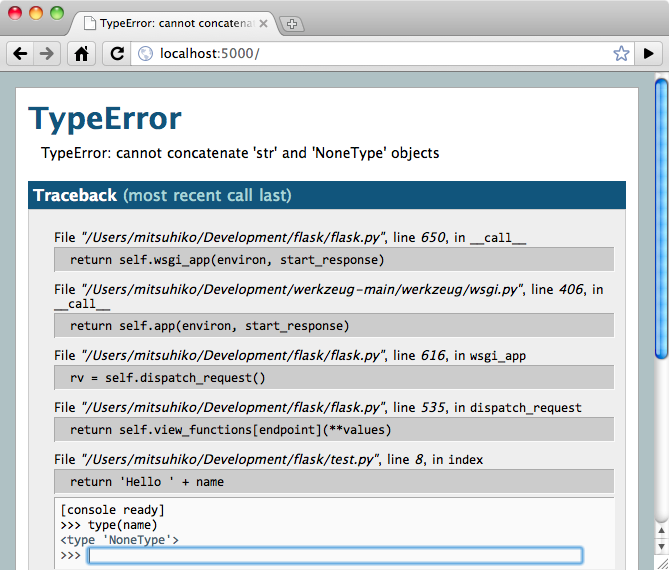
\includegraphics{debugger.png}\hfill}

想使用其他调试器?请参阅 {\hyperref[errorhandling:working-with-debuggers]{\emph{使用调试器}}} 。


\section{路由}
\label{quickstart:id4}
现代 web 应用都使用漂亮的 URL ,有助于人们记忆,对于使用网速较慢的移动设备尤其
有利。如果用户可以不通过点击首页而直达所需要的页面,那么这个网页会更得到用户的
青睐,提高回头率。

如前文所述, {\hyperref[api:flask.Flask.route]{\code{route()}}} 装饰器用于把一个函数绑定到一个 URL 。
下面是一些基本的例子:

\begin{Verbatim}[commandchars=\\\{\}]
\PYG{n+nd}{@app.route}\PYG{p}{(}\PYG{l+s}{\PYGZsq{}}\PYG{l+s}{/}\PYG{l+s}{\PYGZsq{}}\PYG{p}{)}
\PYG{k}{def} \PYG{n+nf}{index}\PYG{p}{(}\PYG{p}{)}\PYG{p}{:}
    \PYG{k}{return} \PYG{l+s}{\PYGZsq{}}\PYG{l+s}{Index Page}\PYG{l+s}{\PYGZsq{}}

\PYG{n+nd}{@app.route}\PYG{p}{(}\PYG{l+s}{\PYGZsq{}}\PYG{l+s}{/hello}\PYG{l+s}{\PYGZsq{}}\PYG{p}{)}
\PYG{k}{def} \PYG{n+nf}{hello}\PYG{p}{(}\PYG{p}{)}\PYG{p}{:}
    \PYG{k}{return} \PYG{l+s}{\PYGZsq{}}\PYG{l+s}{Hello World}\PYG{l+s}{\PYGZsq{}}
\end{Verbatim}

但是能做的不仅仅是这些!你可以动态变化 URL 的某些部分,还可以为一个函数指定多个
规则。


\subsection{变更规则}
\label{quickstart:id5}
通过 URL 的一部分标记为 \code{\textless{}variable\_name\textgreater{}} 就可以在 URL 中添加变量。标记的部分
会作为关键字参数传递给函数。通过使用 \code{\textless{}converter:variable\_name\textgreater{}} ,可以选择性
的加上一个转换器,为变量指定规则。请看下面的例子:

\begin{Verbatim}[commandchars=\\\{\}]
\PYG{n+nd}{@app.route}\PYG{p}{(}\PYG{l+s}{\PYGZsq{}}\PYG{l+s}{/user/\PYGZlt{}username\PYGZgt{}}\PYG{l+s}{\PYGZsq{}}\PYG{p}{)}
\PYG{k}{def} \PYG{n+nf}{show\PYGZus{}user\PYGZus{}profile}\PYG{p}{(}\PYG{n}{username}\PYG{p}{)}\PYG{p}{:}
    \PYG{c}{\PYGZsh{} show the user profile for that user}
    \PYG{k}{return} \PYG{l+s}{\PYGZsq{}}\PYG{l+s}{User }\PYG{l+s+si}{\PYGZpc{}s}\PYG{l+s}{\PYGZsq{}} \PYG{o}{\PYGZpc{}} \PYG{n}{username}

\PYG{n+nd}{@app.route}\PYG{p}{(}\PYG{l+s}{\PYGZsq{}}\PYG{l+s}{/post/\PYGZlt{}int:post\PYGZus{}id\PYGZgt{}}\PYG{l+s}{\PYGZsq{}}\PYG{p}{)}
\PYG{k}{def} \PYG{n+nf}{show\PYGZus{}post}\PYG{p}{(}\PYG{n}{post\PYGZus{}id}\PYG{p}{)}\PYG{p}{:}
    \PYG{c}{\PYGZsh{} show the post with the given id, the id is an integer}
    \PYG{k}{return} \PYG{l+s}{\PYGZsq{}}\PYG{l+s}{Post }\PYG{l+s+si}{\PYGZpc{}d}\PYG{l+s}{\PYGZsq{}} \PYG{o}{\PYGZpc{}} \PYG{n}{post\PYGZus{}id}
\end{Verbatim}

现有的转换器有:

\begin{tabulary}{\linewidth}{|L|L|}
\hline

\emph{int}
 & 
接受整数
\\\hline

\emph{float}
 & 
接受浮点数
\\\hline

\emph{path}
 & 
和缺省情况相同,但也接受斜杠
\\\hline
\end{tabulary}


\begin{notice}{note}{唯一的 URL / 重定向行为}

Flask 的 URL 规则都是基于 Werkzeug 的路由模块的。其背后的理念是保证漂亮的
外观和唯一的 URL 。这个理念来自于 Apache 和更早期的服务器。

假设有如下两条规则:

\begin{Verbatim}[commandchars=\\\{\}]
\PYG{n+nd}{@app.route}\PYG{p}{(}\PYG{l+s}{\PYGZsq{}}\PYG{l+s}{/projects/}\PYG{l+s}{\PYGZsq{}}\PYG{p}{)}
\PYG{k}{def} \PYG{n+nf}{projects}\PYG{p}{(}\PYG{p}{)}\PYG{p}{:}
    \PYG{k}{return} \PYG{l+s}{\PYGZsq{}}\PYG{l+s}{The project page}\PYG{l+s}{\PYGZsq{}}

\PYG{n+nd}{@app.route}\PYG{p}{(}\PYG{l+s}{\PYGZsq{}}\PYG{l+s}{/about}\PYG{l+s}{\PYGZsq{}}\PYG{p}{)}
\PYG{k}{def} \PYG{n+nf}{about}\PYG{p}{(}\PYG{p}{)}\PYG{p}{:}
    \PYG{k}{return} \PYG{l+s}{\PYGZsq{}}\PYG{l+s}{The about page}\PYG{l+s}{\PYGZsq{}}
\end{Verbatim}

它们看上去很相近,不同之处在于 URL \emph{定义} 中尾部的斜杠。第一个例子中
\emph{prjects} 的 URL 是中规中举的,尾部有一个斜杠,看起来就如同一个文件夹。访问
一个没有斜杠结尾的 URL 时 Flask 会自动进行重定向,帮你在尾部加上一个斜杠。

但是在第二个例子中, URL 没有尾部斜杠,因此其行为表现与一个文件类似。如果
访问这个 URL 时添加了尾部斜杠就会得到一个 404 错误。

为什么这样做?因为这样可以使用户在忘记使用尾部斜杠时继续访问相关的 URL 。
这种重定向行为与 Apache 和其他服务器一致。同时, URL 仍保持唯一,帮助搜索
引擎不重复索引同一页面。
\end{notice}


\subsection{URL 构建}
\label{quickstart:url-building}\label{quickstart:url}
如果可以匹配 URL ,那么 Flask 也可以生成 URL 吗?当然可以。
{\hyperref[api:flask.url_for]{\code{url\_for()}}} 函数就是用于构建指定函数的 URL 的。它把函数名称作为
第一个参数,其余参数对应 URL 中的变量。未知变量将添加到 URL 中作为查询参数。
例如:

\begin{Verbatim}[commandchars=\\\{\}]
\PYG{g+gp}{\PYGZgt{}\PYGZgt{}\PYGZgt{} }\PYG{k+kn}{from} \PYG{n+nn}{flask} \PYG{k+kn}{import} \PYG{n}{Flask}\PYG{p}{,} \PYG{n}{url\PYGZus{}for}
\PYG{g+gp}{\PYGZgt{}\PYGZgt{}\PYGZgt{} }\PYG{n}{app} \PYG{o}{=} \PYG{n}{Flask}\PYG{p}{(}\PYG{n}{\PYGZus{}\PYGZus{}name\PYGZus{}\PYGZus{}}\PYG{p}{)}
\PYG{g+gp}{\PYGZgt{}\PYGZgt{}\PYGZgt{} }\PYG{n+nd}{@app.route}\PYG{p}{(}\PYG{l+s}{\PYGZsq{}}\PYG{l+s}{/}\PYG{l+s}{\PYGZsq{}}\PYG{p}{)}
\PYG{g+gp}{... }\PYG{k}{def} \PYG{n+nf}{index}\PYG{p}{(}\PYG{p}{)}\PYG{p}{:} \PYG{k}{pass}
\PYG{g+gp}{...}
\PYG{g+gp}{\PYGZgt{}\PYGZgt{}\PYGZgt{} }\PYG{n+nd}{@app.route}\PYG{p}{(}\PYG{l+s}{\PYGZsq{}}\PYG{l+s}{/login}\PYG{l+s}{\PYGZsq{}}\PYG{p}{)}
\PYG{g+gp}{... }\PYG{k}{def} \PYG{n+nf}{login}\PYG{p}{(}\PYG{p}{)}\PYG{p}{:} \PYG{k}{pass}
\PYG{g+gp}{...}
\PYG{g+gp}{\PYGZgt{}\PYGZgt{}\PYGZgt{} }\PYG{n+nd}{@app.route}\PYG{p}{(}\PYG{l+s}{\PYGZsq{}}\PYG{l+s}{/user/\PYGZlt{}username\PYGZgt{}}\PYG{l+s}{\PYGZsq{}}\PYG{p}{)}
\PYG{g+gp}{... }\PYG{k}{def} \PYG{n+nf}{profile}\PYG{p}{(}\PYG{n}{username}\PYG{p}{)}\PYG{p}{:} \PYG{k}{pass}
\PYG{g+gp}{...}
\PYG{g+gp}{\PYGZgt{}\PYGZgt{}\PYGZgt{} }\PYG{k}{with} \PYG{n}{app}\PYG{o}{.}\PYG{n}{test\PYGZus{}request\PYGZus{}context}\PYG{p}{(}\PYG{p}{)}\PYG{p}{:}
\PYG{g+gp}{... } \PYG{k}{print} \PYG{n}{url\PYGZus{}for}\PYG{p}{(}\PYG{l+s}{\PYGZsq{}}\PYG{l+s}{index}\PYG{l+s}{\PYGZsq{}}\PYG{p}{)}
\PYG{g+gp}{... } \PYG{k}{print} \PYG{n}{url\PYGZus{}for}\PYG{p}{(}\PYG{l+s}{\PYGZsq{}}\PYG{l+s}{login}\PYG{l+s}{\PYGZsq{}}\PYG{p}{)}
\PYG{g+gp}{... } \PYG{k}{print} \PYG{n}{url\PYGZus{}for}\PYG{p}{(}\PYG{l+s}{\PYGZsq{}}\PYG{l+s}{login}\PYG{l+s}{\PYGZsq{}}\PYG{p}{,} \PYG{n+nb}{next}\PYG{o}{=}\PYG{l+s}{\PYGZsq{}}\PYG{l+s}{/}\PYG{l+s}{\PYGZsq{}}\PYG{p}{)}
\PYG{g+gp}{... } \PYG{k}{print} \PYG{n}{url\PYGZus{}for}\PYG{p}{(}\PYG{l+s}{\PYGZsq{}}\PYG{l+s}{profile}\PYG{l+s}{\PYGZsq{}}\PYG{p}{,} \PYG{n}{username}\PYG{o}{=}\PYG{l+s}{\PYGZsq{}}\PYG{l+s}{John Doe}\PYG{l+s}{\PYGZsq{}}\PYG{p}{)}
\PYG{g+gp}{...}
\PYG{g+go}{/}
\PYG{g+go}{/login}
\PYG{g+go}{/login?next=/}
\PYG{g+go}{/user/John\PYGZpc{}20Doe}
\end{Verbatim}

(例子中还使用下文要讲到的 {\hyperref[api:flask.Flask.test_request_context]{\code{test\_request\_context()}}} 方法。这个
方法的作用是告诉 Flask 我们正在处理一个请求,而实际上也许我们正处在交互
Python shell 之中,并没有真正的请求。详见下面的 {\hyperref[quickstart:context-locals]{\emph{本地环境}}} )。

为什么不在把 URL 写死在模板中,反而要动态构建?有三个很好的理由:
\begin{enumerate}
\item {} 
反向解析通常比硬编码 URL 更直观。同时,更重要的是你可以只在一个地方改变
URL ,而不用到处乱找。

\item {} 
URL 创建会为你处理特殊字符的转义和 Unicode 数据,不用你操心。

\item {} 
如果你的应用是放在 URL 根路径之外的地方(如在 \code{/myapplication} 中,不在
\code{/} 中), {\hyperref[api:flask.url_for]{\code{url\_for()}}} 会为你妥善处理。

\end{enumerate}


\subsection{HTTP 方法}
\label{quickstart:http}
HTTP ( web 应用使用的协议)) 协议中有访问 URL 的不同方法。缺省情况下,一个路由
只回应 \emph{GET} 请求,但是可以通过 \emph{methods} 参数使用不同方法。例如:

\begin{Verbatim}[commandchars=\\\{\}]
\PYG{n+nd}{@app.route}\PYG{p}{(}\PYG{l+s}{\PYGZsq{}}\PYG{l+s}{/login}\PYG{l+s}{\PYGZsq{}}\PYG{p}{,} \PYG{n}{methods}\PYG{o}{=}\PYG{p}{[}\PYG{l+s}{\PYGZsq{}}\PYG{l+s}{GET}\PYG{l+s}{\PYGZsq{}}\PYG{p}{,} \PYG{l+s}{\PYGZsq{}}\PYG{l+s}{POST}\PYG{l+s}{\PYGZsq{}}\PYG{p}{]}\PYG{p}{)}
\PYG{k}{def} \PYG{n+nf}{login}\PYG{p}{(}\PYG{p}{)}\PYG{p}{:}
    \PYG{k}{if} \PYG{n}{request}\PYG{o}{.}\PYG{n}{method} \PYG{o}{==} \PYG{l+s}{\PYGZsq{}}\PYG{l+s}{POST}\PYG{l+s}{\PYGZsq{}}\PYG{p}{:}
        \PYG{n}{do\PYGZus{}the\PYGZus{}login}\PYG{p}{(}\PYG{p}{)}
    \PYG{k}{else}\PYG{p}{:}
        \PYG{n}{show\PYGZus{}the\PYGZus{}login\PYGZus{}form}\PYG{p}{(}\PYG{p}{)}
\end{Verbatim}

如果当前使用的是 \emph{GET} 方法,会自动添加 \emph{HEAD} ,你不必亲自操刀。同时还会确保
\emph{HEAD} 请求按照 \href{http://www.ietf.org/rfc/rfc2068.txt}{HTTP RFC} (说明 HTTP 协议的文档)的要求来处理,因此你可以
完全忽略这部分 HTTP 规范。与 Flask 0.6 一样, \emph{OPTIONS} 自动为你处理好。

完全不懂 HTTP 方法?没关系,这里给你速成培训一下:

HTTP 方法(通常也被称为“动作”)告诉服务器一个页面请求要 \emph{做} 什么。以下是常见
的方法:
\begin{description}
\item[{\emph{GET}}] \leavevmode
浏览器告诉服务器只要 \emph{得到} 页面上的信息并发送这些信息。这可能是最常见的
方法。

\item[{\emph{HEAD}}] \leavevmode
浏览器告诉服务器想要得到信息,但是只要得到 \emph{信息头} 就行了,页面内容不要。
一个应用应该像接受到一个 \emph{GET} 请求一样运行,但是不传递实际的内容。在
Flask 中,你根本不必理会这个,下层的 Werkzeug 库会为你处理好。

\item[{\emph{POST}}] \leavevmode
浏览器告诉服务器想要向 URL  \emph{发表} 一些新的信息,服务器必须确保数据被保存好
且只保存了一次。 HTML 表单实际上就是使用这个访求向服务器传送数据的。

\item[{\emph{PUT}}] \leavevmode
与 \emph{POST} 方法类似,不同的是服务器可能触发多次储存过程而把旧的值覆盖掉。你
可能会问这样做有什么用?这样做是有原因的。假设在传输过程中连接丢失的情况
下,一个处于浏览器和服务器之间的系统可以在不中断的情况下安全地接收第二次
请求。在这种情况下,使用 \emph{POST} 方法就无法做到了,因为它只被触发一次。

\item[{\emph{DELETE}}] \leavevmode
删除给定位置的信息。

\item[{\emph{OPTIONS}}] \leavevmode
为客户端提供一个查询 URL 支持哪些方法的捷径。从 Flask 0.6 开始,自动为你
实现了这个方法。

\end{description}

有趣的是在 HTML4 和 XHTML1 中,表单只能使用 \emph{GET} 和 \emph{POST} 方法。但是
JavaScript 和未来的 HTML 标准中可以使用其他的方法。此外, HTTP 近来已经变得相当
流行,浏览器不再只是唯一使用 HTTP 的客户端。比如许多版本控制系统也使用 HTTP 。


\section{静态文件}
\label{quickstart:http-rfc}\label{quickstart:id6}
动态的 web 应用也需要静态文件,一般是 CSS 和 JavaScript 文件。理想情况下你的
服务器已经配置好了为你的提供静态文件的服务。在开发过程中, Flask 也能做好这个
工作。只要在你的包或模块旁边创建一个名为 \emph{static} 的文件夹就行了。静态文件位于
应用的 \emph{/static} 中。

使用选定的 \code{'static'} 端点就可以生成相应的 URL 。:

\begin{Verbatim}[commandchars=\\\{\}]
\PYG{n}{url\PYGZus{}for}\PYG{p}{(}\PYG{l+s}{\PYGZsq{}}\PYG{l+s}{static}\PYG{l+s}{\PYGZsq{}}\PYG{p}{,} \PYG{n}{filename}\PYG{o}{=}\PYG{l+s}{\PYGZsq{}}\PYG{l+s}{style.css}\PYG{l+s}{\PYGZsq{}}\PYG{p}{)}
\end{Verbatim}

这个静态文件在文件系统中的位置应该是 \code{static/style.css} 。


\section{渲染模板}
\label{quickstart:id7}
在 Python 内部生成 HTML 不好玩,且相当笨拙。因为你必须自己负责 HTML 转义,以
确保应用的安全。因此, Flask 自动为你配置的 \href{http://jinja.pocoo.org/2/}{Jinja2} 模板引擎。

使用 {\hyperref[api:flask.render_template]{\code{render\_template()}}} 方法可以渲染模板,你只要提供模板名称和需要
作为参数传递给模板的变量就行了。下面是一个简单的模板渲染例子:

\begin{Verbatim}[commandchars=\\\{\}]
\PYG{k+kn}{from} \PYG{n+nn}{flask} \PYG{k+kn}{import} \PYG{n}{render\PYGZus{}template}

\PYG{n+nd}{@app.route}\PYG{p}{(}\PYG{l+s}{\PYGZsq{}}\PYG{l+s}{/hello/}\PYG{l+s}{\PYGZsq{}}\PYG{p}{)}
\PYG{n+nd}{@app.route}\PYG{p}{(}\PYG{l+s}{\PYGZsq{}}\PYG{l+s}{/hello/\PYGZlt{}name\PYGZgt{}}\PYG{l+s}{\PYGZsq{}}\PYG{p}{)}
\PYG{k}{def} \PYG{n+nf}{hello}\PYG{p}{(}\PYG{n}{name}\PYG{o}{=}\PYG{n+nb+bp}{None}\PYG{p}{)}\PYG{p}{:}
    \PYG{k}{return} \PYG{n}{render\PYGZus{}template}\PYG{p}{(}\PYG{l+s}{\PYGZsq{}}\PYG{l+s}{hello.html}\PYG{l+s}{\PYGZsq{}}\PYG{p}{,} \PYG{n}{name}\PYG{o}{=}\PYG{n}{name}\PYG{p}{)}
\end{Verbatim}

Flask 会在 \emph{templates} 文件夹内寻找模板。因此,如果你的应用是一个模块,那么模板
文件夹应该在模块旁边;如果是一个包,那么就应该在包里面:

\textbf{情形 1}: 一个模块:

\begin{Verbatim}[commandchars=\\\{\}]
/application.py
/templates
    /hello.html
\end{Verbatim}

\textbf{情形 2}: 一个包:

\begin{Verbatim}[commandchars=\\\{\}]
/application
    /\_\_init\_\_.py
    /templates
        /hello.html
\end{Verbatim}

你可以充分使用 Jinja2 模板引擎的威力。更多内容,详见官方 \href{http://jinja.pocoo.org/2/documentation/templates}{Jinja2 模板文档} 。

模板举例:

\begin{Verbatim}[commandchars=\\\{\}]
\PYG{c+cp}{\PYGZlt{}!doctype html\PYGZgt{}}
\PYG{n+nt}{\PYGZlt{}title}\PYG{n+nt}{\PYGZgt{}}Hello from Flask\PYG{n+nt}{\PYGZlt{}/title\PYGZgt{}}
\PYG{c+cp}{\PYGZob{}\PYGZpc{}} \PYG{k}{if} \PYG{n+nv}{name} \PYG{c+cp}{\PYGZpc{}\PYGZcb{}}
  \PYG{n+nt}{\PYGZlt{}h1}\PYG{n+nt}{\PYGZgt{}}Hello \PYG{c+cp}{\PYGZob{}\PYGZob{}} \PYG{n+nv}{name} \PYG{c+cp}{\PYGZcb{}\PYGZcb{}}!\PYG{n+nt}{\PYGZlt{}/h1\PYGZgt{}}
\PYG{c+cp}{\PYGZob{}\PYGZpc{}} \PYG{k}{else} \PYG{c+cp}{\PYGZpc{}\PYGZcb{}}
  \PYG{n+nt}{\PYGZlt{}h1}\PYG{n+nt}{\PYGZgt{}}Hello World!\PYG{n+nt}{\PYGZlt{}/h1\PYGZgt{}}
\PYG{c+cp}{\PYGZob{}\PYGZpc{}} \PYG{k}{endif} \PYG{c+cp}{\PYGZpc{}\PYGZcb{}}
\end{Verbatim}

在模板内部你也可以访问 {\hyperref[api:flask.request]{\code{request}}} 、{\hyperref[api:flask.session]{\code{session}}} 和
{\hyperref[api:flask.g]{\code{g}}} \footnote{
不理解什么是 {\hyperref[api:flask.g]{\code{g}}} 对象?它是某个可以根据需要储存信息的
东西。更多信息参见 {\hyperref[api:flask.g]{\code{g}}} 对象的文档和 {\hyperref[patterns/sqlite3:sqlite3]{\emph{在 Flask 中使用 SQLite 3}}} 文档。
} 对象,以及 {\hyperref[api:flask.get_flashed_messages]{\code{get\_flashed\_messages()}}} 函数。

模板在继承使用的情况下尤其有用,其工作原理 {\hyperref[patterns/templateinheritance:template-inheritance]{\emph{模板继承}}} 方案
文档。简单的说,模板继承可以使每个页面的特定元素(如页头,导航,页尾)保持
一致。

自动转义默认开启。因此,如果 \emph{name} 包含 HTML ,那么会被自动转义。如果你可以
信任某个变量,且知道它是安全的 HTML (例如变量来自一个把 wiki 标记转换为 HTML
的模块),那么可以使用 \code{Markup} 类把它标记为安全的。否则请在模板
中使用 \code{\textbar{}safe} 过滤器。更多例子参见 Jinja 2 文档。

下面简单介绍一下 \code{Markup} 类的工作方式:

\begin{Verbatim}[commandchars=\\\{\}]
\PYG{g+gp}{\PYGZgt{}\PYGZgt{}\PYGZgt{} }\PYG{k+kn}{from} \PYG{n+nn}{flask} \PYG{k+kn}{import} \PYG{n}{Markup}
\PYG{g+gp}{\PYGZgt{}\PYGZgt{}\PYGZgt{} }\PYG{n}{Markup}\PYG{p}{(}\PYG{l+s}{\PYGZsq{}}\PYG{l+s}{\PYGZlt{}strong\PYGZgt{}Hello }\PYG{l+s+si}{\PYGZpc{}s}\PYG{l+s}{!\PYGZlt{}/strong\PYGZgt{}}\PYG{l+s}{\PYGZsq{}}\PYG{p}{)} \PYG{o}{\PYGZpc{}} \PYG{l+s}{\PYGZsq{}}\PYG{l+s}{\PYGZlt{}blink\PYGZgt{}hacker\PYGZlt{}/blink\PYGZgt{}}\PYG{l+s}{\PYGZsq{}}
\PYG{g+go}{Markup(u\PYGZsq{}\PYGZlt{}strong\PYGZgt{}Hello \PYGZam{}lt;blink\PYGZam{}gt;hacker\PYGZam{}lt;/blink\PYGZam{}gt;!\PYGZlt{}/strong\PYGZgt{}\PYGZsq{})}
\PYG{g+gp}{\PYGZgt{}\PYGZgt{}\PYGZgt{} }\PYG{n}{Markup}\PYG{o}{.}\PYG{n}{escape}\PYG{p}{(}\PYG{l+s}{\PYGZsq{}}\PYG{l+s}{\PYGZlt{}blink\PYGZgt{}hacker\PYGZlt{}/blink\PYGZgt{}}\PYG{l+s}{\PYGZsq{}}\PYG{p}{)}
\PYG{g+go}{Markup(u\PYGZsq{}\PYGZam{}lt;blink\PYGZam{}gt;hacker\PYGZam{}lt;/blink\PYGZam{}gt;\PYGZsq{})}
\PYG{g+gp}{\PYGZgt{}\PYGZgt{}\PYGZgt{} }\PYG{n}{Markup}\PYG{p}{(}\PYG{l+s}{\PYGZsq{}}\PYG{l+s}{\PYGZlt{}em\PYGZgt{}Marked up\PYGZlt{}/em\PYGZgt{} \PYGZam{}raquo; HTML}\PYG{l+s}{\PYGZsq{}}\PYG{p}{)}\PYG{o}{.}\PYG{n}{striptags}\PYG{p}{(}\PYG{p}{)}
\PYG{g+go}{u\PYGZsq{}Marked up \PYGZbs{}xbb HTML\PYGZsq{}}
\end{Verbatim}
在 0.5 版更改.

\section{操作请求数据}
\label{quickstart:id11}
对于 web 应用来说对客户端向服务器发送的数据作出响应很重要。在 Flask 中由全局
对象 {\hyperref[api:flask.request]{\code{request}}} 来提供请求信息。如果你有一些 Python 基础,那么可能
会奇怪:既然这个对象是全局的,怎么还能保持线程安全?答案是本地环境:


\subsection{本地环境}
\label{quickstart:id12}\label{quickstart:context-locals}
\begin{notice}{note}{内部信息}

如果你想了解其工作原理和如何测试,请阅读本节,否则可以跳过本节。
\end{notice}

某些对象在 Flask 中是全局对象,但是不是通常意义下的全局对象。这些对象实际上是
特定环境下本地对象的代理。真拗口!但还是很容易理解的。

设想现在处于处理线程的环境中。一个请求进来了,服务器决定生成一个新线程(或者
叫其他什么名称的东西,这个下层的东西能够处理包括线程在内的并发系统)。当
Flask 开始其内部请求处理时会把当前线程作为活动环境,并把当前应用和 WSGI 环境
绑定到这个环境(线程)。它以一种聪明的方式使得一个应用可以在不中断的情况下
调用另一个应用。

这对你有什么用?基本上你可以完全不必理会。这个只有在做单元测试时才有用。在测试
时会遇到由于没有请求对象而导致依赖于请求的代码会突然崩溃的情况。对策是自己创建
一个请求对象并绑定到环境。最简单的单元测试解决方案是使用
{\hyperref[api:flask.Flask.test_request_context]{\code{test\_request\_context()}}} 环境管理器。通过使用 \emph{with} 语句可以
绑定一个测试请求,以便于交互。例如:

\begin{Verbatim}[commandchars=\\\{\}]
\PYG{k+kn}{from} \PYG{n+nn}{flask} \PYG{k+kn}{import} \PYG{n}{request}

\PYG{k}{with} \PYG{n}{app}\PYG{o}{.}\PYG{n}{test\PYGZus{}request\PYGZus{}context}\PYG{p}{(}\PYG{l+s}{\PYGZsq{}}\PYG{l+s}{/hello}\PYG{l+s}{\PYGZsq{}}\PYG{p}{,} \PYG{n}{method}\PYG{o}{=}\PYG{l+s}{\PYGZsq{}}\PYG{l+s}{POST}\PYG{l+s}{\PYGZsq{}}\PYG{p}{)}\PYG{p}{:}
    \PYG{c}{\PYGZsh{} now you can do something with the request until the}
    \PYG{c}{\PYGZsh{} end of the with block, such as basic assertions:}
    \PYG{k}{assert} \PYG{n}{request}\PYG{o}{.}\PYG{n}{path} \PYG{o}{==} \PYG{l+s}{\PYGZsq{}}\PYG{l+s}{/hello}\PYG{l+s}{\PYGZsq{}}
    \PYG{k}{assert} \PYG{n}{request}\PYG{o}{.}\PYG{n}{method} \PYG{o}{==} \PYG{l+s}{\PYGZsq{}}\PYG{l+s}{POST}\PYG{l+s}{\PYGZsq{}}
\end{Verbatim}

另一种方式是把整个 WSGI 环境传递给 {\hyperref[api:flask.Flask.request_context]{\code{request\_context()}}} 方法:

\begin{Verbatim}[commandchars=\\\{\}]
\PYG{k+kn}{from} \PYG{n+nn}{flask} \PYG{k+kn}{import} \PYG{n}{request}

\PYG{k}{with} \PYG{n}{app}\PYG{o}{.}\PYG{n}{request\PYGZus{}context}\PYG{p}{(}\PYG{n}{environ}\PYG{p}{)}\PYG{p}{:}
    \PYG{k}{assert} \PYG{n}{request}\PYG{o}{.}\PYG{n}{method} \PYG{o}{==} \PYG{l+s}{\PYGZsq{}}\PYG{l+s}{POST}\PYG{l+s}{\PYGZsq{}}
\end{Verbatim}


\subsection{请求对象}
\label{quickstart:id13}
请求对象在 API 一节中有详细说明这里不细谈(参见 {\hyperref[api:flask.request]{\code{request}}} )。
这里简略地谈一下最常见的操作。首先,你必须从 \emph{flask} 模块导入请求对象:

\begin{Verbatim}[commandchars=\\\{\}]
\PYG{k+kn}{from} \PYG{n+nn}{flask} \PYG{k+kn}{import} \PYG{n}{request}
\end{Verbatim}

通过使用 \code{method} 属性可以操作当前请求方法,通过使用
\code{form} 属性处理表单数据。以下是使用两个属性的例子:

\begin{Verbatim}[commandchars=\\\{\}]
\PYG{n+nd}{@app.route}\PYG{p}{(}\PYG{l+s}{\PYGZsq{}}\PYG{l+s}{/login}\PYG{l+s}{\PYGZsq{}}\PYG{p}{,} \PYG{n}{methods}\PYG{o}{=}\PYG{p}{[}\PYG{l+s}{\PYGZsq{}}\PYG{l+s}{POST}\PYG{l+s}{\PYGZsq{}}\PYG{p}{,} \PYG{l+s}{\PYGZsq{}}\PYG{l+s}{GET}\PYG{l+s}{\PYGZsq{}}\PYG{p}{]}\PYG{p}{)}
\PYG{k}{def} \PYG{n+nf}{login}\PYG{p}{(}\PYG{p}{)}\PYG{p}{:}
    \PYG{n}{error} \PYG{o}{=} \PYG{n+nb+bp}{None}
    \PYG{k}{if} \PYG{n}{request}\PYG{o}{.}\PYG{n}{method} \PYG{o}{==} \PYG{l+s}{\PYGZsq{}}\PYG{l+s}{POST}\PYG{l+s}{\PYGZsq{}}\PYG{p}{:}
        \PYG{k}{if} \PYG{n}{valid\PYGZus{}login}\PYG{p}{(}\PYG{n}{request}\PYG{o}{.}\PYG{n}{form}\PYG{p}{[}\PYG{l+s}{\PYGZsq{}}\PYG{l+s}{username}\PYG{l+s}{\PYGZsq{}}\PYG{p}{]}\PYG{p}{,}
                       \PYG{n}{request}\PYG{o}{.}\PYG{n}{form}\PYG{p}{[}\PYG{l+s}{\PYGZsq{}}\PYG{l+s}{password}\PYG{l+s}{\PYGZsq{}}\PYG{p}{]}\PYG{p}{)}\PYG{p}{:}
            \PYG{k}{return} \PYG{n}{log\PYGZus{}the\PYGZus{}user\PYGZus{}in}\PYG{p}{(}\PYG{n}{request}\PYG{o}{.}\PYG{n}{form}\PYG{p}{[}\PYG{l+s}{\PYGZsq{}}\PYG{l+s}{username}\PYG{l+s}{\PYGZsq{}}\PYG{p}{]}\PYG{p}{)}
        \PYG{k}{else}\PYG{p}{:}
            \PYG{n}{error} \PYG{o}{=} \PYG{l+s}{\PYGZsq{}}\PYG{l+s}{Invalid username/password}\PYG{l+s}{\PYGZsq{}}
    \PYG{c}{\PYGZsh{} 如果请求访求是 GET 或验证未通过就会执行下面的代码}
    \PYG{k}{return} \PYG{n}{render\PYGZus{}template}\PYG{p}{(}\PYG{l+s}{\PYGZsq{}}\PYG{l+s}{login.html}\PYG{l+s}{\PYGZsq{}}\PYG{p}{,} \PYG{n}{error}\PYG{o}{=}\PYG{n}{error}\PYG{p}{)}
\end{Verbatim}

当 \emph{form} 属性中不存在这个键时会发生什么?会引发一个 \href{http://docs.python.org/dev/library/exceptions.html\#KeyError}{\code{KeyError}} 。如果你不
像捕捉一个标准错误一样捕捉 \href{http://docs.python.org/dev/library/exceptions.html\#KeyError}{\code{KeyError}} ,那么会显示一个 HTTP 400 Bad
Request 错误页面。因此,多数情况下你不必处理这个问题。

要操作 URL (如 \code{?key=value} )中提交的参数可以使用
\code{args} 属性:

\begin{Verbatim}[commandchars=\\\{\}]
\PYG{n}{searchword} \PYG{o}{=} \PYG{n}{request}\PYG{o}{.}\PYG{n}{args}\PYG{o}{.}\PYG{n}{get}\PYG{p}{(}\PYG{l+s}{\PYGZsq{}}\PYG{l+s}{key}\PYG{l+s}{\PYGZsq{}}\PYG{p}{,} \PYG{l+s}{\PYGZsq{}}\PYG{l+s}{\PYGZsq{}}\PYG{p}{)}
\end{Verbatim}

用户可能会改变 URL 导致出现一个 400 请求出错页面,这样降低了用户友好度。因此,
我们推荐使用 \emph{get} 或通过捕捉 \emph{KeyError} 来访问 URL 参数。

完整的请求对象方法和属性参见 {\hyperref[api:flask.request]{\code{request}}} 文档。


\subsection{文件上传}
\label{quickstart:id14}
用 Flask 处理文件上传很容易,只要确保不要忘记在你的 HTML 表单中设置
\code{enctype="multipart/form-data"} 属性就可以了。否则浏览器将不会传送你的文件。

已上传的文件被储存在内存或文件系统的临时位置。你可以通过请求对象
\code{files} 属性来访问上传的文件。每个上传的文件都储存在这个
字典型属性中。这个属性基本和标准 Python \code{file} 对象一样,另外多出一个
用于把上传文件保存到服务器的文件系统中的
\href{http://werkzeug.pocoo.org/docs/datastructures/\#werkzeug.datastructures.FileStorage.save}{\code{save()}} 方法。下例展示其如何运作:

\begin{Verbatim}[commandchars=\\\{\}]
\PYG{k+kn}{from} \PYG{n+nn}{flask} \PYG{k+kn}{import} \PYG{n}{request}

\PYG{n+nd}{@app.route}\PYG{p}{(}\PYG{l+s}{\PYGZsq{}}\PYG{l+s}{/upload}\PYG{l+s}{\PYGZsq{}}\PYG{p}{,} \PYG{n}{methods}\PYG{o}{=}\PYG{p}{[}\PYG{l+s}{\PYGZsq{}}\PYG{l+s}{GET}\PYG{l+s}{\PYGZsq{}}\PYG{p}{,} \PYG{l+s}{\PYGZsq{}}\PYG{l+s}{POST}\PYG{l+s}{\PYGZsq{}}\PYG{p}{]}\PYG{p}{)}
\PYG{k}{def} \PYG{n+nf}{upload\PYGZus{}file}\PYG{p}{(}\PYG{p}{)}\PYG{p}{:}
    \PYG{k}{if} \PYG{n}{request}\PYG{o}{.}\PYG{n}{method} \PYG{o}{==} \PYG{l+s}{\PYGZsq{}}\PYG{l+s}{POST}\PYG{l+s}{\PYGZsq{}}\PYG{p}{:}
        \PYG{n}{f} \PYG{o}{=} \PYG{n}{request}\PYG{o}{.}\PYG{n}{files}\PYG{p}{[}\PYG{l+s}{\PYGZsq{}}\PYG{l+s}{the\PYGZus{}file}\PYG{l+s}{\PYGZsq{}}\PYG{p}{]}
        \PYG{n}{f}\PYG{o}{.}\PYG{n}{save}\PYG{p}{(}\PYG{l+s}{\PYGZsq{}}\PYG{l+s}{/var/www/uploads/uploaded\PYGZus{}file.txt}\PYG{l+s}{\PYGZsq{}}\PYG{p}{)}
    \PYG{o}{.}\PYG{o}{.}\PYG{o}{.}
\end{Verbatim}

如果想要知道文件上传之前其在客户端系统中的名称,可以使用
\href{http://werkzeug.pocoo.org/docs/datastructures/\#werkzeug.datastructures.FileStorage.filename}{\code{filename}} 属性。但是请牢记这个值是
可以伪造的,永远不要信任这个值。如果想要把客户端的文件名作为服务器上的文件名,
可以通过 Werkzeug 提供的 \href{http://werkzeug.pocoo.org/docs/utils/\#werkzeug.utils.secure\_filename}{\code{secure\_filename()}} 函数:

\begin{Verbatim}[commandchars=\\\{\}]
\PYG{k+kn}{from} \PYG{n+nn}{flask} \PYG{k+kn}{import} \PYG{n}{request}
\PYG{k+kn}{from} \PYG{n+nn}{werkzeug} \PYG{k+kn}{import} \PYG{n}{secure\PYGZus{}filename}

\PYG{n+nd}{@app.route}\PYG{p}{(}\PYG{l+s}{\PYGZsq{}}\PYG{l+s}{/upload}\PYG{l+s}{\PYGZsq{}}\PYG{p}{,} \PYG{n}{methods}\PYG{o}{=}\PYG{p}{[}\PYG{l+s}{\PYGZsq{}}\PYG{l+s}{GET}\PYG{l+s}{\PYGZsq{}}\PYG{p}{,} \PYG{l+s}{\PYGZsq{}}\PYG{l+s}{POST}\PYG{l+s}{\PYGZsq{}}\PYG{p}{]}\PYG{p}{)}
\PYG{k}{def} \PYG{n+nf}{upload\PYGZus{}file}\PYG{p}{(}\PYG{p}{)}\PYG{p}{:}
    \PYG{k}{if} \PYG{n}{request}\PYG{o}{.}\PYG{n}{method} \PYG{o}{==} \PYG{l+s}{\PYGZsq{}}\PYG{l+s}{POST}\PYG{l+s}{\PYGZsq{}}\PYG{p}{:}
        \PYG{n}{f} \PYG{o}{=} \PYG{n}{request}\PYG{o}{.}\PYG{n}{files}\PYG{p}{[}\PYG{l+s}{\PYGZsq{}}\PYG{l+s}{the\PYGZus{}file}\PYG{l+s}{\PYGZsq{}}\PYG{p}{]}
        \PYG{n}{f}\PYG{o}{.}\PYG{n}{save}\PYG{p}{(}\PYG{l+s}{\PYGZsq{}}\PYG{l+s}{/var/www/uploads/}\PYG{l+s}{\PYGZsq{}} \PYG{o}{+} \PYG{n}{secure\PYGZus{}filename}\PYG{p}{(}\PYG{n}{f}\PYG{o}{.}\PYG{n}{filename}\PYG{p}{)}\PYG{p}{)}
    \PYG{o}{.}\PYG{o}{.}\PYG{o}{.}
\end{Verbatim}

更好的例子参见 {\hyperref[patterns/fileuploads:uploading-files]{\emph{上传文件}}} 方案。


\subsection{Cookies}
\label{quickstart:cookies}
要访问 cookies ,可以使用 {\hyperref[api:flask.Request.cookies]{\code{cookies}}} 属性。可以使用请求对象
的 {\hyperref[api:flask.Response.set_cookie]{\code{set\_cookie}}} 方法来设置 cookies 。请求对象的
{\hyperref[api:flask.Request.cookies]{\code{cookies}}} 属性是一个包含了客户端传输的所有 cookies 的字典。
在 Flask 中,如果能够使用 {\hyperref[quickstart:sessions]{\emph{会话}}} ,那么就不要直接使用 cookies ,因为
会话比较安全一些。

读取 cookies:

\begin{Verbatim}[commandchars=\\\{\}]
\PYG{k+kn}{from} \PYG{n+nn}{flask} \PYG{k+kn}{import} \PYG{n}{request}

\PYG{n+nd}{@app.route}\PYG{p}{(}\PYG{l+s}{\PYGZsq{}}\PYG{l+s}{/}\PYG{l+s}{\PYGZsq{}}\PYG{p}{)}
\PYG{k}{def} \PYG{n+nf}{index}\PYG{p}{(}\PYG{p}{)}\PYG{p}{:}
    \PYG{n}{username} \PYG{o}{=} \PYG{n}{request}\PYG{o}{.}\PYG{n}{cookies}\PYG{o}{.}\PYG{n}{get}\PYG{p}{(}\PYG{l+s}{\PYGZsq{}}\PYG{l+s}{username}\PYG{l+s}{\PYGZsq{}}\PYG{p}{)}
    \PYG{c}{\PYGZsh{} 使用 cookies.get(key) 来代替 cookies[key] ,}
    \PYG{c}{\PYGZsh{} 以避免当 cookie 不存在时引发 KeyError 。}
\end{Verbatim}

储存 cookies:

\begin{Verbatim}[commandchars=\\\{\}]
\PYG{k+kn}{from} \PYG{n+nn}{flask} \PYG{k+kn}{import} \PYG{n}{make\PYGZus{}response}

\PYG{n+nd}{@app.route}\PYG{p}{(}\PYG{l+s}{\PYGZsq{}}\PYG{l+s}{/}\PYG{l+s}{\PYGZsq{}}\PYG{p}{)}
\PYG{k}{def} \PYG{n+nf}{index}\PYG{p}{(}\PYG{p}{)}\PYG{p}{:}
    \PYG{n}{resp} \PYG{o}{=} \PYG{n}{make\PYGZus{}response}\PYG{p}{(}\PYG{n}{render\PYGZus{}template}\PYG{p}{(}\PYG{o}{.}\PYG{o}{.}\PYG{o}{.}\PYG{p}{)}\PYG{p}{)}
    \PYG{n}{resp}\PYG{o}{.}\PYG{n}{set\PYGZus{}cookie}\PYG{p}{(}\PYG{l+s}{\PYGZsq{}}\PYG{l+s}{username}\PYG{l+s}{\PYGZsq{}}\PYG{p}{,} \PYG{l+s}{\PYGZsq{}}\PYG{l+s}{the username}\PYG{l+s}{\PYGZsq{}}\PYG{p}{)}
    \PYG{k}{return} \PYG{n}{resp}
\end{Verbatim}

注意, cookies 设置在响应对象上。通常只是从视图函数返回字符串, Flask 会把它们
转换为响应对象。如果你想显式地转换,那么可以使用 {\hyperref[api:flask.make_response]{\code{make\_response()}}}
函数,然后再修改它。

使用 {\hyperref[patterns/deferredcallbacks:deferred-callbacks]{\emph{延迟的请求回调}}} 方案可以在没有响应对象的情况下设置一个 cookie 。

同时可以参见 {\hyperref[quickstart:about-responses]{\emph{关于响应}}} 。


\section{重定向和错误}
\label{quickstart:id15}
使用 {\hyperref[api:flask.redirect]{\code{redirect()}}} 函数可以重定向。使用 {\hyperref[api:flask.abort]{\code{abort()}}} 可以及早
从错误代码中脱身。举例说明:

\begin{Verbatim}[commandchars=\\\{\}]
\PYG{k+kn}{from} \PYG{n+nn}{flask} \PYG{k+kn}{import} \PYG{n}{abort}\PYG{p}{,} \PYG{n}{redirect}\PYG{p}{,} \PYG{n}{url\PYGZus{}for}

\PYG{n+nd}{@app.route}\PYG{p}{(}\PYG{l+s}{\PYGZsq{}}\PYG{l+s}{/}\PYG{l+s}{\PYGZsq{}}\PYG{p}{)}
\PYG{k}{def} \PYG{n+nf}{index}\PYG{p}{(}\PYG{p}{)}\PYG{p}{:}
    \PYG{k}{return} \PYG{n}{redirect}\PYG{p}{(}\PYG{n}{url\PYGZus{}for}\PYG{p}{(}\PYG{l+s}{\PYGZsq{}}\PYG{l+s}{login}\PYG{l+s}{\PYGZsq{}}\PYG{p}{)}\PYG{p}{)}

\PYG{n+nd}{@app.route}\PYG{p}{(}\PYG{l+s}{\PYGZsq{}}\PYG{l+s}{/login}\PYG{l+s}{\PYGZsq{}}\PYG{p}{)}
\PYG{k}{def} \PYG{n+nf}{login}\PYG{p}{(}\PYG{p}{)}\PYG{p}{:}
    \PYG{n}{abort}\PYG{p}{(}\PYG{l+m+mi}{401}\PYG{p}{)}
    \PYG{n}{this\PYGZus{}is\PYGZus{}never\PYGZus{}executed}\PYG{p}{(}\PYG{p}{)}
\end{Verbatim}

上例实际上是没有意义的,它让一个用户从索引页重定向到一个无法访问的页面(401
表示禁止访问)。但是上例可以说明重定向和出错跳出是如何工作的。

缺省情况下每种出错代码都会对应显示一个黑白的出错页面。使用
{\hyperref[api:flask.Flask.errorhandler]{\code{errorhandler()}}} 装饰器可以定制出错页面:

\begin{Verbatim}[commandchars=\\\{\}]
\PYG{k+kn}{from} \PYG{n+nn}{flask} \PYG{k+kn}{import} \PYG{n}{render\PYGZus{}template}

\PYG{n+nd}{@app.errorhandler}\PYG{p}{(}\PYG{l+m+mi}{404}\PYG{p}{)}
\PYG{k}{def} \PYG{n+nf}{page\PYGZus{}not\PYGZus{}found}\PYG{p}{(}\PYG{n}{error}\PYG{p}{)}\PYG{p}{:}
    \PYG{k}{return} \PYG{n}{render\PYGZus{}template}\PYG{p}{(}\PYG{l+s}{\PYGZsq{}}\PYG{l+s}{page\PYGZus{}not\PYGZus{}found.html}\PYG{l+s}{\PYGZsq{}}\PYG{p}{)}\PYG{p}{,} \PYG{l+m+mi}{404}
\end{Verbatim}

注意 {\hyperref[api:flask.render_template]{\code{render\_template()}}} 后面的 \code{404} ,这表示页面对就的出错代码是
404 ,即页面不存在。缺省情况下 200 表示一切正常。


\section{关于响应}
\label{quickstart:about-responses}\label{quickstart:id16}
视图函数的返回值会自动转换为一个响应对象。如果返回值是一个字符串,那么会被转换
为一个包含作为响应体的字符串、一个 \code{200 OK} 出错代码 和一个 \code{text/html}
MIME 类型的响应对象。以下是转换的规则:
\begin{enumerate}
\item {} 
如果视图要返回的是一个响应对象,那么就直接返回它。

\item {} 
如果要返回的是一个字符串,那么根据这个字符串和缺省参数生成一个用于返回的
响应对象。

\item {} 
如果要返回的是一个元组,那么元组中的项目可以提供额外的信息。元组中必须至少
包含一个项目,且项目应当由 \code{(response, status, headers)} 组成。 \emph{status}
的值会重载状态代码, \emph{headers} 是一个由额外头部值组成的列表或字典。

\item {} 
如果以上都不是,那么 Flask 会假定返回值是一个有效的 WSGI 应用并把它转换为
一个响应对象。

\end{enumerate}

如果想要在视图内部掌控响应对象的结果,那么可以使用
{\hyperref[api:flask.make_response]{\code{make\_response()}}} 函数。

设想有如下视图:

\begin{Verbatim}[commandchars=\\\{\}]
\PYG{n+nd}{@app.errorhandler}\PYG{p}{(}\PYG{l+m+mi}{404}\PYG{p}{)}
\PYG{k}{def} \PYG{n+nf}{not\PYGZus{}found}\PYG{p}{(}\PYG{n}{error}\PYG{p}{)}\PYG{p}{:}
    \PYG{k}{return} \PYG{n}{render\PYGZus{}template}\PYG{p}{(}\PYG{l+s}{\PYGZsq{}}\PYG{l+s}{error.html}\PYG{l+s}{\PYGZsq{}}\PYG{p}{)}\PYG{p}{,} \PYG{l+m+mi}{404}
\end{Verbatim}

可以使用 {\hyperref[api:flask.make_response]{\code{make\_response()}}} 包裹返回表达式,获得结果。对结果进行修改
后再返回:

\begin{Verbatim}[commandchars=\\\{\}]
\PYG{n+nd}{@app.errorhandler}\PYG{p}{(}\PYG{l+m+mi}{404}\PYG{p}{)}
\PYG{k}{def} \PYG{n+nf}{not\PYGZus{}found}\PYG{p}{(}\PYG{n}{error}\PYG{p}{)}\PYG{p}{:}
    \PYG{n}{resp} \PYG{o}{=} \PYG{n}{make\PYGZus{}response}\PYG{p}{(}\PYG{n}{render\PYGZus{}template}\PYG{p}{(}\PYG{l+s}{\PYGZsq{}}\PYG{l+s}{error.html}\PYG{l+s}{\PYGZsq{}}\PYG{p}{)}\PYG{p}{,} \PYG{l+m+mi}{404}\PYG{p}{)}
    \PYG{n}{resp}\PYG{o}{.}\PYG{n}{headers}\PYG{p}{[}\PYG{l+s}{\PYGZsq{}}\PYG{l+s}{X\PYGZhy{}Something}\PYG{l+s}{\PYGZsq{}}\PYG{p}{]} \PYG{o}{=} \PYG{l+s}{\PYGZsq{}}\PYG{l+s}{A value}\PYG{l+s}{\PYGZsq{}}
    \PYG{k}{return} \PYG{n}{resp}
\end{Verbatim}


\section{会话}
\label{quickstart:id17}\label{quickstart:sessions}
除了请求对象之外还有一种称为 {\hyperref[api:flask.session]{\code{session}}} 的对象,允许你在不同请求
之间储存信息。这个对象相当于用密钥签名加密的 cookie ,即用户可以查看你的
cookie ,但是如果没有密钥就无法修改它。

使用会话之前你必须设置一个密钥。举例说明:

\begin{Verbatim}[commandchars=\\\{\}]
\PYG{k+kn}{from} \PYG{n+nn}{flask} \PYG{k+kn}{import} \PYG{n}{Flask}\PYG{p}{,} \PYG{n}{session}\PYG{p}{,} \PYG{n}{redirect}\PYG{p}{,} \PYG{n}{url\PYGZus{}for}\PYG{p}{,} \PYG{n}{escape}\PYG{p}{,} \PYG{n}{request}

\PYG{n}{app} \PYG{o}{=} \PYG{n}{Flask}\PYG{p}{(}\PYG{n}{\PYGZus{}\PYGZus{}name\PYGZus{}\PYGZus{}}\PYG{p}{)}

\PYG{n+nd}{@app.route}\PYG{p}{(}\PYG{l+s}{\PYGZsq{}}\PYG{l+s}{/}\PYG{l+s}{\PYGZsq{}}\PYG{p}{)}
\PYG{k}{def} \PYG{n+nf}{index}\PYG{p}{(}\PYG{p}{)}\PYG{p}{:}
    \PYG{k}{if} \PYG{l+s}{\PYGZsq{}}\PYG{l+s}{username}\PYG{l+s}{\PYGZsq{}} \PYG{o+ow}{in} \PYG{n}{session}\PYG{p}{:}
        \PYG{k}{return} \PYG{l+s}{\PYGZsq{}}\PYG{l+s}{Logged in as }\PYG{l+s+si}{\PYGZpc{}s}\PYG{l+s}{\PYGZsq{}} \PYG{o}{\PYGZpc{}} \PYG{n}{escape}\PYG{p}{(}\PYG{n}{session}\PYG{p}{[}\PYG{l+s}{\PYGZsq{}}\PYG{l+s}{username}\PYG{l+s}{\PYGZsq{}}\PYG{p}{]}\PYG{p}{)}
    \PYG{k}{return} \PYG{l+s}{\PYGZsq{}}\PYG{l+s}{You are not logged in}\PYG{l+s}{\PYGZsq{}}

\PYG{n+nd}{@app.route}\PYG{p}{(}\PYG{l+s}{\PYGZsq{}}\PYG{l+s}{/login}\PYG{l+s}{\PYGZsq{}}\PYG{p}{,} \PYG{n}{methods}\PYG{o}{=}\PYG{p}{[}\PYG{l+s}{\PYGZsq{}}\PYG{l+s}{GET}\PYG{l+s}{\PYGZsq{}}\PYG{p}{,} \PYG{l+s}{\PYGZsq{}}\PYG{l+s}{POST}\PYG{l+s}{\PYGZsq{}}\PYG{p}{]}\PYG{p}{)}
\PYG{k}{def} \PYG{n+nf}{login}\PYG{p}{(}\PYG{p}{)}\PYG{p}{:}
    \PYG{k}{if} \PYG{n}{request}\PYG{o}{.}\PYG{n}{method} \PYG{o}{==} \PYG{l+s}{\PYGZsq{}}\PYG{l+s}{POST}\PYG{l+s}{\PYGZsq{}}\PYG{p}{:}
        \PYG{n}{session}\PYG{p}{[}\PYG{l+s}{\PYGZsq{}}\PYG{l+s}{username}\PYG{l+s}{\PYGZsq{}}\PYG{p}{]} \PYG{o}{=} \PYG{n}{request}\PYG{o}{.}\PYG{n}{form}\PYG{p}{[}\PYG{l+s}{\PYGZsq{}}\PYG{l+s}{username}\PYG{l+s}{\PYGZsq{}}\PYG{p}{]}
        \PYG{k}{return} \PYG{n}{redirect}\PYG{p}{(}\PYG{n}{url\PYGZus{}for}\PYG{p}{(}\PYG{l+s}{\PYGZsq{}}\PYG{l+s}{index}\PYG{l+s}{\PYGZsq{}}\PYG{p}{)}\PYG{p}{)}
    \PYG{k}{return} \PYG{l+s}{\PYGZsq{}\PYGZsq{}\PYGZsq{}}
\PYG{l+s}{        \PYGZlt{}form action=}\PYG{l+s}{\PYGZdq{}}\PYG{l+s}{\PYGZdq{}}\PYG{l+s}{ method=}\PYG{l+s}{\PYGZdq{}}\PYG{l+s}{post}\PYG{l+s}{\PYGZdq{}}\PYG{l+s}{\PYGZgt{}}
\PYG{l+s}{            \PYGZlt{}p\PYGZgt{}\PYGZlt{}input type=text name=username\PYGZgt{}}
\PYG{l+s}{            \PYGZlt{}p\PYGZgt{}\PYGZlt{}input type=submit value=Login\PYGZgt{}}
\PYG{l+s}{        \PYGZlt{}/form\PYGZgt{}}
\PYG{l+s}{    }\PYG{l+s}{\PYGZsq{}\PYGZsq{}\PYGZsq{}}

\PYG{n+nd}{@app.route}\PYG{p}{(}\PYG{l+s}{\PYGZsq{}}\PYG{l+s}{/logout}\PYG{l+s}{\PYGZsq{}}\PYG{p}{)}
\PYG{k}{def} \PYG{n+nf}{logout}\PYG{p}{(}\PYG{p}{)}\PYG{p}{:}
    \PYG{c}{\PYGZsh{} 如果会话中有用户名就删除它。}
    \PYG{n}{session}\PYG{o}{.}\PYG{n}{pop}\PYG{p}{(}\PYG{l+s}{\PYGZsq{}}\PYG{l+s}{username}\PYG{l+s}{\PYGZsq{}}\PYG{p}{,} \PYG{n+nb+bp}{None}\PYG{p}{)}
    \PYG{k}{return} \PYG{n}{redirect}\PYG{p}{(}\PYG{n}{url\PYGZus{}for}\PYG{p}{(}\PYG{l+s}{\PYGZsq{}}\PYG{l+s}{index}\PYG{l+s}{\PYGZsq{}}\PYG{p}{)}\PYG{p}{)}

\PYG{c}{\PYGZsh{} 设置密钥,复杂一点:}
\PYG{n}{app}\PYG{o}{.}\PYG{n}{secret\PYGZus{}key} \PYG{o}{=} \PYG{l+s}{\PYGZsq{}}\PYG{l+s}{A0Zr98j/3yX R\PYGZti{}XHH!jmN]LWX/,?RT}\PYG{l+s}{\PYGZsq{}}
\end{Verbatim}

这里用到的 {\hyperref[api:flask.escape]{\code{escape()}}} 是用来转义的。如果不使用模板引擎就可以像上例
一样使用这个函数来转义。

\begin{notice}{note}{如果生成一个好的密钥}

生成随机数的关键在于一个好的随机种子,困此一个好的密钥应当有足够的随机性。
你的操作系统可以使用一个随机生成器来生成一个好的随机种子:

\begin{Verbatim}[commandchars=\\\{\}]
\PYG{g+gp}{\PYGZgt{}\PYGZgt{}\PYGZgt{} }\PYG{k+kn}{import} \PYG{n+nn}{os}
\PYG{g+gp}{\PYGZgt{}\PYGZgt{}\PYGZgt{} }\PYG{n}{os}\PYG{o}{.}\PYG{n}{urandom}\PYG{p}{(}\PYG{l+m+mi}{24}\PYG{p}{)}
\PYG{g+go}{\PYGZsq{}\PYGZbs{}xfd\PYGZob{}H\PYGZbs{}xe5\PYGZlt{}\PYGZbs{}x95\PYGZbs{}xf9\PYGZbs{}xe3\PYGZbs{}x96.5\PYGZbs{}xd1\PYGZbs{}x01O\PYGZlt{}!\PYGZbs{}xd5\PYGZbs{}xa2\PYGZbs{}xa0\PYGZbs{}x9fR\PYGZdq{}\PYGZbs{}xa1\PYGZbs{}xa8\PYGZsq{}}
\end{Verbatim}

只要复制这个随机种子到你的代码中就行了。
\end{notice}

基于 cookie 的会话的说明: Flask 会把会话对象中的值储存在 cookie 中。在打开
cookie 的情况下,如果你访问会话对象中没有的值,那么会得到模糊的错误信息:请检查
页面 cookie 的大小是否与网络浏览器所支持的大小一致。


\section{消息闪现}
\label{quickstart:id18}
一个好的应用和用户接口都有良好的反馈,否则到后来用户就会讨厌这个应用。 Flask
通过闪现系统来提供了一个易用的反馈方式。闪现系统的基本工作原理是在请求结束时
记录一个消息,提供且只提供给下一个请求使用。通常通过一个布局模板来展现闪现的
消息。

{\hyperref[api:flask.flash]{\code{flash()}}} 用于闪现一个消息。在模板中,使用
{\hyperref[api:flask.get_flashed_messages]{\code{get\_flashed\_messages()}}} 来操作消息。完整的例子参见
{\hyperref[patterns/flashing:message-flashing-pattern]{\emph{消息闪现}}} 。


\section{日志}
\label{quickstart:id19}0.3 新版功能.
有时候可能会遇到数据出错需要纠正的情况。例如因为用户篡改了数据或客户端代码出错
而导致一个客户端代码向服务器发送了明显错误的 HTTP 请求。多数时候在类似情况下
返回 \code{400 Bad Request} 就没事了,但也有不会返回的时候,而代码还得继续运行
下去。

这时候就需要使用日志来记录这些不正常的东西了。自从 Flask 0.3 后就已经为你配置好
了一个日志工具。

以下是一些日志调用示例:

\begin{Verbatim}[commandchars=\\\{\}]
\PYG{n}{app}\PYG{o}{.}\PYG{n}{logger}\PYG{o}{.}\PYG{n}{debug}\PYG{p}{(}\PYG{l+s}{\PYGZsq{}}\PYG{l+s}{A value for debugging}\PYG{l+s}{\PYGZsq{}}\PYG{p}{)}
\PYG{n}{app}\PYG{o}{.}\PYG{n}{logger}\PYG{o}{.}\PYG{n}{warning}\PYG{p}{(}\PYG{l+s}{\PYGZsq{}}\PYG{l+s}{A warning occurred (}\PYG{l+s+si}{\PYGZpc{}d}\PYG{l+s}{ apples)}\PYG{l+s}{\PYGZsq{}}\PYG{p}{,} \PYG{l+m+mi}{42}\PYG{p}{)}
\PYG{n}{app}\PYG{o}{.}\PYG{n}{logger}\PYG{o}{.}\PYG{n}{error}\PYG{p}{(}\PYG{l+s}{\PYGZsq{}}\PYG{l+s}{An error occurred}\PYG{l+s}{\PYGZsq{}}\PYG{p}{)}
\end{Verbatim}

{\hyperref[api:flask.Flask.logger]{\code{logger}}} 是一个标准的 Python \href{http://docs.python.org/dev/library/logging.html\#logging.Logger}{\code{Logger}} 类,
更多信息详见官方的 \href{http://docs.python.org/library/logging.html}{logging 文档} 。


\section{集成 WSGI 中间件}
\label{quickstart:wsgi}
如果想要在应用中添加一个 WSGI 中间件,那么可以包装内部的 WSGI 应用。假设为了
解决 lighttpd 的错误,你要使用一个来自 Werkzeug 包的中间件,那么可以这样做:

\begin{Verbatim}[commandchars=\\\{\}]
\PYG{k+kn}{from} \PYG{n+nn}{werkzeug.contrib.fixers} \PYG{k+kn}{import} \PYG{n}{LighttpdCGIRootFix}
\PYG{n}{app}\PYG{o}{.}\PYG{n}{wsgi\PYGZus{}app} \PYG{o}{=} \PYG{n}{LighttpdCGIRootFix}\PYG{p}{(}\PYG{n}{app}\PYG{o}{.}\PYG{n}{wsgi\PYGZus{}app}\PYG{p}{)}
\end{Verbatim}


\section{部署到一个网络服务器}
\label{quickstart:quickstart-deployment}\label{quickstart:id20}
准备好发布你的新 Flask 应用了吗?作为本文的一个圆满结尾,你可以立即把应用部署到
一个主机上。下面介绍的是如何把小项目部署到免费主机上。
\begin{itemize}
\item {} 
\href{http://devcenter.heroku.com/articles/python}{把 Flask 部署到 Heroku}

\item {} 
\href{http://docs.dotcloud.com/services/python/}{把 WSGI 部署到 dotCloud} 的
\href{http://flask.pocoo.org/snippets/48/}{Flask 应用注意点}

\end{itemize}

其他可以部署 Flask 应用的地方:
\begin{itemize}
\item {} 
\href{http://flask.pocoo.org/snippets/65/}{把 Flask 部署到 Webfaction}

\item {} 
\href{https://github.com/kamalgill/flask-appengine-template}{把 Flask 部署到 Google App Engine}

\item {} 
\href{http://flask.pocoo.org/snippets/89/}{用 Localtunnel 分离你的本地服务器}

\end{itemize}

如果拥有自己的独立主机,参见《 {\hyperref[deploying/index:deployment]{\emph{部署方式}}} 》。


\chapter{教程}
\label{tutorial/index::doc}\label{tutorial/index:tutorial}\label{tutorial/index:id1}
想要用 Python 和 Flask 开发应用吗?让我们来边看例子边学习。本教程中我们将会创建
一个微博应用。这个应用只支持单一用户,只能创建文本条目,也没有不能订阅和评论,
但是已经具备一个初学者需要掌握的功能。这个应用只需要使用 Flask 和 SQLite ,
SQLite 是 Python 自带的。

如果你想要事先下载完整的源代码或者用于比较,请查看 \href{http://github.com/mitsuhiko/flask/tree/master/examples/flaskr/}{示例源代码} 。


\section{Flaskr 介绍}
\label{tutorial/introduction:flaskr}\label{tutorial/introduction::doc}\label{tutorial/introduction:tutorial-introduction}
我们把教程中的博客应用称为 flaskr ,当然你也可以随便取一个没有 web-2.0 气息的
名字  ;)  它的基本功能如下:
\begin{enumerate}
\item {} 
让用户可以根据配置文件中的信息登录和注销。只支持一个用户。

\item {} 
用户登录以后可以添加新的博客条目。条目由文本标题和支持 HTML 代码的内容组成。
因为我们信任用户,所以不对内容中的 HTML 进行净化处理。

\item {} 
页面以倒序(越新的在越上面)显示所有条目。并且用户登录以后可以在这个页面添加
新的条目。

\end{enumerate}

我们直接在应用中使用 SQLite3 ,因为在这种规模的应用中 SQlite3 已经够用了。如果
是大型应用,那么就有必要使用能够好的处理数据库连接的 \href{http://www.sqlalchemy.org/}{SQLAlchemy} 了,它可以
同时对应多种数据库,并做其他更多的事情。如果你的数据更适合使用 NoSQL 数据库,
那么也可以考虑使用某种流行的 NoSQL 数据库。

这是教程应用完工后的截图:

{\hfill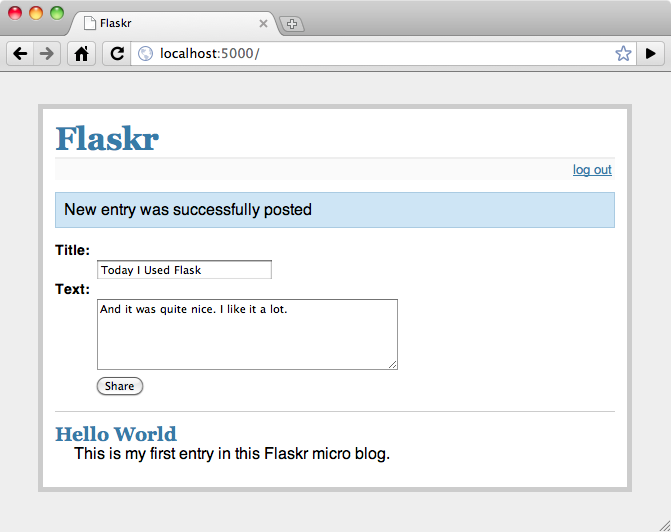
\includegraphics{flaskr.png}\hfill}

下面请阅读 {\hyperref[tutorial/folders:tutorial-folders]{\emph{步骤 0 :创建文件夹}}} 。


\section{步骤 0 :创建文件夹}
\label{tutorial/folders:sqlalchemy}\label{tutorial/folders::doc}\label{tutorial/folders:tutorial-folders}\label{tutorial/folders:id1}
在开始之前需要为应用创建下列文件夹:

\begin{Verbatim}[commandchars=\\\{\}]
/flaskr
    /static
    /templates
\end{Verbatim}

\emph{flaskr} 文件夹不是一个 Python 包,只是一个用来存放我们文件的地方。我们将把以后
要用到的数据库模式和主模块放在这个文件夹中。 \emph{static} 文件夹中的文件是用于被
应用用户通过 \emph{HTTP} 访问的文件,主要是 CSS 和 javascript 文件。 Flask 将会在
\emph{templates} 文件夹中搜索 \href{http://jinja.pocoo.org/2/}{Jinja2} 模板,所有在教程中的模板都放在
\emph{templates} 文件夹中。

下面请阅读 {\hyperref[tutorial/schema:tutorial-schema]{\emph{步骤 1 :数据库模式}}} 。


\section{步骤 1 :数据库模式}
\label{tutorial/schema::doc}\label{tutorial/schema:jinja2}\label{tutorial/schema:tutorial-schema}\label{tutorial/schema:id1}
首先我们要创建数据库模式。本应用只需要使用一张表,并且由于我们使用 SQLite ,
所以这一步非常简单。把以下内容保存为 \emph{schema.sql} 文件并放在我们上一步创建的
\emph{flaskr} 文件夹中就行了:

\begin{Verbatim}[commandchars=\\\{\}]
\PYG{k}{drop} \PYG{k}{table} \PYG{n}{if} \PYG{k}{exists} \PYG{n}{entries}\PYG{p}{;}
\PYG{k}{create} \PYG{k}{table} \PYG{n}{entries} \PYG{p}{(}
  \PYG{n}{id} \PYG{n+nb}{integer} \PYG{k}{primary} \PYG{k}{key} \PYG{n}{autoincrement}\PYG{p}{,}
  \PYG{n}{title} \PYG{n}{string} \PYG{k}{not} \PYG{k}{null}\PYG{p}{,}
  \PYG{n+nb}{text} \PYG{n}{string} \PYG{k}{not} \PYG{k}{null}
\PYG{p}{)}\PYG{p}{;}
\end{Verbatim}

这个模式只有一张名为 \emph{entries} 的表,表中的字段为 \emph{id} 、 \emph{title} 和 \emph{text} 。
\emph{id} 是主键,是自增整数型字段,别外两个字段是非空的字符串型字段。

下面请阅读 {\hyperref[tutorial/setup:tutorial-setup]{\emph{步骤 2 :应用构建代码}}} 。


\section{步骤 2 :应用构建代码}
\label{tutorial/setup:tutorial-setup}\label{tutorial/setup::doc}\label{tutorial/setup:id1}
现在我们已经准备好了数据库模式了,下面来创建应用模块。我们把模块命名为
\emph{flaskr.py} ,并放在 \emph{flaskr} 文件夹中。为了方便初学者学习,我们把库的导入与
相关配置放在了一起。对于小型应用来说,可以把配置直接放在模块中。但是更加清晰的
方案是把配置放在一个独立的 \emph{.ini} 或 \emph{.py} 文件中,并在模块中导入配置的值。

In \emph{flaskr.py} 文件中:

\begin{Verbatim}[commandchars=\\\{\}]
\PYG{c}{\PYGZsh{} all the imports}
\PYG{k+kn}{import} \PYG{n+nn}{sqlite3}
\PYG{k+kn}{from} \PYG{n+nn}{flask} \PYG{k+kn}{import} \PYG{n}{Flask}\PYG{p}{,} \PYG{n}{request}\PYG{p}{,} \PYG{n}{session}\PYG{p}{,} \PYG{n}{g}\PYG{p}{,} \PYG{n}{redirect}\PYG{p}{,} \PYG{n}{url\PYGZus{}for}\PYG{p}{,} \PYGZbs{}
     \PYG{n}{abort}\PYG{p}{,} \PYG{n}{render\PYGZus{}template}\PYG{p}{,} \PYG{n}{flash}

\PYG{c}{\PYGZsh{} configuration}
\PYG{n}{DATABASE} \PYG{o}{=} \PYG{l+s}{\PYGZsq{}}\PYG{l+s}{/tmp/flaskr.db}\PYG{l+s}{\PYGZsq{}}
\PYG{n}{DEBUG} \PYG{o}{=} \PYG{n+nb+bp}{True}
\PYG{n}{SECRET\PYGZus{}KEY} \PYG{o}{=} \PYG{l+s}{\PYGZsq{}}\PYG{l+s}{development key}\PYG{l+s}{\PYGZsq{}}
\PYG{n}{USERNAME} \PYG{o}{=} \PYG{l+s}{\PYGZsq{}}\PYG{l+s}{admin}\PYG{l+s}{\PYGZsq{}}
\PYG{n}{PASSWORD} \PYG{o}{=} \PYG{l+s}{\PYGZsq{}}\PYG{l+s}{default}\PYG{l+s}{\PYGZsq{}}
\end{Verbatim}

接着创建真正的应用,并用同一文件中的配置来初始化,In \emph{flaskr.py} 文件中:

\begin{Verbatim}[commandchars=\\\{\}]
\PYG{c}{\PYGZsh{} create our little application :)}
\PYG{n}{app} \PYG{o}{=} \PYG{n}{Flask}\PYG{p}{(}\PYG{n}{\PYGZus{}\PYGZus{}name\PYGZus{}\PYGZus{}}\PYG{p}{)}
\PYG{n}{app}\PYG{o}{.}\PYG{n}{config}\PYG{o}{.}\PYG{n}{from\PYGZus{}object}\PYG{p}{(}\PYG{n}{\PYGZus{}\PYGZus{}name\PYGZus{}\PYGZus{}}\PYG{p}{)}
\end{Verbatim}

{\hyperref[api:flask.Config.from_object]{\code{from\_object()}}} 会查看给定的对象(如果该对象是一个字符串就会
直接导入它),搜索对象中所有变量名均为大字字母的变量。在我们的应用中,已经配置
写在前面了。你可以把这些配置放到一个独立的文件中。

通常,好的做法是从一个配置文件中导入配置,我们使用
{\hyperref[api:flask.Config.from_envvar]{\code{from\_envvar()}}} 来完成这个工作,把上面的
{\hyperref[api:flask.Config.from_object]{\code{from\_object()}}} 一行替换为:

\begin{Verbatim}[commandchars=\\\{\}]
\PYG{n}{app}\PYG{o}{.}\PYG{n}{config}\PYG{o}{.}\PYG{n}{from\PYGZus{}envvar}\PYG{p}{(}\PYG{l+s}{\PYGZsq{}}\PYG{l+s}{FLASKR\PYGZus{}SETTINGS}\PYG{l+s}{\PYGZsq{}}\PYG{p}{,} \PYG{n}{silent}\PYG{o}{=}\PYG{n+nb+bp}{True}\PYG{p}{)}
\end{Verbatim}

这样做就可以设置一个 \index{FLASKR\_SETTINGS}\index{环境变量!FLASKR\_SETTINGS}\code{FLASKR\_SETTINGS} 的环境变量来指定一个配置文件,并
根据该文件来重载缺省的配置。 silent 开关的作用是告诉 Flask 如果没有这个环境变量
不要报错。

\emph{secret\_key} (密钥)用于保持客户端会话安全,请谨慎地选择密钥,并尽可能的使它
复杂而且不容易被猜到。 DEBUG 标志用于开关交互调试器。因为调试模式允许用户执行
服务器上的代码,所以 \emph{永远不要在生产环境中打开调试模式} !

我们还添加了一个方便连接指定数据库的方法。这个方法可以用于在请求时打开连接,也
可以用于 Python 交互终端或代码中。以后会派上用场。

\begin{Verbatim}[commandchars=\\\{\}]
\PYG{k}{def} \PYG{n+nf}{connect\PYGZus{}db}\PYG{p}{(}\PYG{p}{)}\PYG{p}{:}
    \PYG{k}{return} \PYG{n}{sqlite3}\PYG{o}{.}\PYG{n}{connect}\PYG{p}{(}\PYG{n}{app}\PYG{o}{.}\PYG{n}{config}\PYG{p}{[}\PYG{l+s}{\PYGZsq{}}\PYG{l+s}{DATABASE}\PYG{l+s}{\PYGZsq{}}\PYG{p}{]}\PYG{p}{)}
\end{Verbatim}

最后,在文件末尾添加以单机方式启动服务器的代码:

\begin{Verbatim}[commandchars=\\\{\}]
\PYG{k}{if} \PYG{n}{\PYGZus{}\PYGZus{}name\PYGZus{}\PYGZus{}} \PYG{o}{==} \PYG{l+s}{\PYGZsq{}}\PYG{l+s}{\PYGZus{}\PYGZus{}main\PYGZus{}\PYGZus{}}\PYG{l+s}{\PYGZsq{}}\PYG{p}{:}
    \PYG{n}{app}\PYG{o}{.}\PYG{n}{run}\PYG{p}{(}\PYG{p}{)}
\end{Verbatim}

到些为止,我们可以顺利运行应用了。输入以下命令开始运行:

\begin{Verbatim}[commandchars=\\\{\}]
python flaskr.py
\end{Verbatim}

你会看到服务器已经运行的信息,其中包含应用访问地址。

因为我们还没创建视图,所以当你在浏览器中访问这个地址时,会得到一个 404 页面未
找到错误。很快我们就会谈到视图,但我们先要弄好数据库。

\begin{notice}{note}{外部可见的服务器}

想让你的服务器被公开访问?详见 {\hyperref[quickstart:public-server]{\emph{外部可见的服务器}}} 。
\end{notice}

下面请阅读 {\hyperref[tutorial/dbinit:tutorial-dbinit]{\emph{步骤 3 :创建数据库}}} 。


\section{步骤 3 :创建数据库}
\label{tutorial/dbinit:tutorial-dbinit}\label{tutorial/dbinit::doc}\label{tutorial/dbinit:id1}
如前所述 Flaskr 是一个数据库驱动的应用,更准确地说是一个关系型数据库驱动的
应用。关系型数据库需要一个数据库模式来定义如何储存信息,因此必须在第一次运行
服务器前创建数据库模式。

使用 \emph{sqlite3} 命令通过管道导入 \emph{schema.sql} 创建模式:

\begin{Verbatim}[commandchars=\\\{\}]
\PYG{n}{sqlite3} \PYG{o}{/}\PYG{n}{tmp}\PYG{o}{/}\PYG{n}{flaskr}\PYG{o}{.}\PYG{n}{db} \PYG{o}{\PYGZlt{}} \PYG{n}{schema}\PYG{o}{.}\PYG{n}{sql}
\end{Verbatim}

上述方法的不足之处是另外需要 sqlite3 命令,但这个命令不是每个系统都有的。而且还
必须提供数据库的路径,容易出错。因此更好的方法是在应用中添加一个数据库初始化
函数。

添加的方法是:首先从 contextlib 库中导入 \href{http://docs.python.org/dev/library/contextlib.html\#contextlib.closing}{\code{contextlib.closing()}} 函数。如果
你使用的是 Python 2.5 ,还必须先打开 \emph{with} 语句( \emph{\_\_future\_\_} 必须第一个
导入):

\begin{Verbatim}[commandchars=\\\{\}]
\PYG{k+kn}{from} \PYG{n+nn}{\PYGZus{}\PYGZus{}future\PYGZus{}\PYGZus{}} \PYG{k+kn}{import} \PYG{n}{with\PYGZus{}statement}
\PYG{k+kn}{from} \PYG{n+nn}{contextlib} \PYG{k+kn}{import} \PYG{n}{closing}
\end{Verbatim}

接下来,可以创建一个用来初始化数据库的 \emph{init\_db} 函数,其中我们使用了先前创建的
\emph{connect\_db} 函数。把这个初始化函数放在 \emph{connect\_db} 函数下面:

\begin{Verbatim}[commandchars=\\\{\}]
\PYG{k}{def} \PYG{n+nf}{init\PYGZus{}db}\PYG{p}{(}\PYG{p}{)}\PYG{p}{:}
    \PYG{k}{with} \PYG{n}{closing}\PYG{p}{(}\PYG{n}{connect\PYGZus{}db}\PYG{p}{(}\PYG{p}{)}\PYG{p}{)} \PYG{k}{as} \PYG{n}{db}\PYG{p}{:}
        \PYG{k}{with} \PYG{n}{app}\PYG{o}{.}\PYG{n}{open\PYGZus{}resource}\PYG{p}{(}\PYG{l+s}{\PYGZsq{}}\PYG{l+s}{schema.sql}\PYG{l+s}{\PYGZsq{}}\PYG{p}{)} \PYG{k}{as} \PYG{n}{f}\PYG{p}{:}
            \PYG{n}{db}\PYG{o}{.}\PYG{n}{cursor}\PYG{p}{(}\PYG{p}{)}\PYG{o}{.}\PYG{n}{executescript}\PYG{p}{(}\PYG{n}{f}\PYG{o}{.}\PYG{n}{read}\PYG{p}{(}\PYG{p}{)}\PYG{p}{)}
        \PYG{n}{db}\PYG{o}{.}\PYG{n}{commit}\PYG{p}{(}\PYG{p}{)}
\end{Verbatim}

\href{http://docs.python.org/dev/library/contextlib.html\#contextlib.closing}{\code{closing()}} 帮助函数允许我们在 \emph{with} 代码块保持数据库连接
打开。应用对象的 {\hyperref[api:flask.Flask.open_resource]{\code{open\_resource()}}} 方法支持也支持这个功能,
所以可以在 \emph{with} 代码块中直接使用。这个函数打开一个位于来源位置(你的
\emph{flaskr} 文件夹)的文件并允许你读取文件的内容。这里我们用于在数据库连接上执行
代码。

当我们连接到数据库时,我们得到一个提供指针的连接对象(本例中的 \emph{db} )。这个
指针有一个方法可以执行完整的代码。最后我们提供要做的修改。 SQLite 3 和其他
事务型数据库只有在显式提交时才会真正提交。

现在可以创建数据库了。打开 Python shell ,导入,调用函数:

\begin{Verbatim}[commandchars=\\\{\}]
\PYG{g+gp}{\PYGZgt{}\PYGZgt{}\PYGZgt{} }\PYG{k+kn}{from} \PYG{n+nn}{flaskr} \PYG{k+kn}{import} \PYG{n}{init\PYGZus{}db}
\PYG{g+gp}{\PYGZgt{}\PYGZgt{}\PYGZgt{} }\PYG{n}{init\PYGZus{}db}\PYG{p}{(}\PYG{p}{)}
\end{Verbatim}

\begin{notice}{note}{故障处理}

如果出现表无法找到的问题,请检查是否写错了函数名称(应该是 \emph{init\_db} ),
是否写错了表名(例如单数复数错误)。
\end{notice}

下面请阅读 {\hyperref[tutorial/dbcon:tutorial-dbcon]{\emph{步骤 4 :请求数据库连接}}} 。


\section{步骤 4 :请求数据库连接}
\label{tutorial/dbcon::doc}\label{tutorial/dbcon:tutorial-dbcon}\label{tutorial/dbcon:id1}
现在我们已经学会如何打开并在代码中使用数据库连接,但是如何优雅地在请求时使用它
呢?我们会在每一个函数中用到数据库连接,因此有必要在请求之前初始化连接,并在
请求之后关闭连接。

Flask 中可以使用 {\hyperref[api:flask.Flask.before_request]{\code{before\_request()}}} 、
{\hyperref[api:flask.Flask.after_request]{\code{after\_request()}}} 和 {\hyperref[api:flask.Flask.teardown_request]{\code{teardown\_request()}}}
装饰器达到这个目的:

\begin{Verbatim}[commandchars=\\\{\}]
\PYG{n+nd}{@app.before\PYGZus{}request}
\PYG{k}{def} \PYG{n+nf}{before\PYGZus{}request}\PYG{p}{(}\PYG{p}{)}\PYG{p}{:}
    \PYG{n}{g}\PYG{o}{.}\PYG{n}{db} \PYG{o}{=} \PYG{n}{connect\PYGZus{}db}\PYG{p}{(}\PYG{p}{)}

\PYG{n+nd}{@app.teardown\PYGZus{}request}
\PYG{k}{def} \PYG{n+nf}{teardown\PYGZus{}request}\PYG{p}{(}\PYG{n}{exception}\PYG{p}{)}\PYG{p}{:}
    \PYG{n}{g}\PYG{o}{.}\PYG{n}{db}\PYG{o}{.}\PYG{n}{close}\PYG{p}{(}\PYG{p}{)}
\end{Verbatim}

使用 {\hyperref[api:flask.Flask.before_request]{\code{before\_request()}}} 装饰的函数会在请求之前调用,且不传递
参数。使用 {\hyperref[api:flask.Flask.after_request]{\code{after\_request()}}} 装饰的函数会在请求之后调用,且
传递发送给客户端响应对象。它们必须传递响应对象,所以在出错的情况下就不会执行。
因此我们就要用到 {\hyperref[api:flask.Flask.teardown_request]{\code{teardown\_request()}}} 装饰器了。这个装饰器下
的函数在响应对象构建后被调用。它们不允许修改请求,并且它们的返回值被忽略。如果
请求过程中出错,那么这个错误会传递给每个函数;否则传递 \emph{None} 。

我们把数据库连接保存在 Flask 提供的特殊的 {\hyperref[api:flask.g]{\code{g}}} 对象中。这个对象与
每一个请求是一一对应的,并且只在函数内部有效。不要在其它对象中储存类似信息,
因为在多线程环境下无效。这个特殊的 {\hyperref[api:flask.g]{\code{g}}} 对象在后台神奇的工作,保证
系统正常运行。

下面请阅读 {\hyperref[tutorial/views:tutorial-views]{\emph{步骤 5 :视图函数}}}.

\begin{notice}{hint}{提示:}
我该把这些代码放在哪里?

如果你按教程一步一步读下来,那么可能会疑惑应该把这个步骤和以后步骤的代码放在
哪里?比较有条理的做法是把这些模块级别的函数放在一起,并把新的
\code{before\_request} 和 \code{teardown\_request} 函数放在前文的 \code{init\_db} 函数
下面(即按照教程的顺序放置)。

如果你已经晕头转向了,那么你可以参考一下 \href{http://github.com/mitsuhiko/flask/tree/master/examples/flaskr/}{示例源代码} 。在 Flask 中,你可以
把应用的所有代码都放在同一个 Python 模块中。但是你没有必要这样做,尤其是当你
的应用 {\hyperref[patterns/packages:larger-applications]{\emph{变大了}}} 的时候,更不应当这样。
\end{notice}


\section{步骤 5 :视图函数}
\label{tutorial/views::doc}\label{tutorial/views:id2}\label{tutorial/views:tutorial-views}\label{tutorial/views:id1}
现在数据库连接弄好了,接站开始写视图函数。我们共需要四个视图函数:


\subsection{显示条目}
\label{tutorial/views:id2}
这个视图显示所有数据库中的条目。它绑定应用的根地址,并从数据库中读取 title 和
text 字段。 id 最大的记录(最新的条目)在最上面。从指针返回的记录集是一个包含
select 语句查询结果的元组。对于教程应用这样的小应用,做到这样就已经够好了。但是
你可能想要把结果转换为字典,具体做法参见 {\hyperref[patterns/sqlite3:easy-querying]{\emph{简化查询}}} 中的例子。

这个视图会把条目作为字典传递给 \emph{show\_entries.html} 模板,并返回渲染结果:

\begin{Verbatim}[commandchars=\\\{\}]
\PYG{n+nd}{@app.route}\PYG{p}{(}\PYG{l+s}{\PYGZsq{}}\PYG{l+s}{/}\PYG{l+s}{\PYGZsq{}}\PYG{p}{)}
\PYG{k}{def} \PYG{n+nf}{show\PYGZus{}entries}\PYG{p}{(}\PYG{p}{)}\PYG{p}{:}
    \PYG{n}{cur} \PYG{o}{=} \PYG{n}{g}\PYG{o}{.}\PYG{n}{db}\PYG{o}{.}\PYG{n}{execute}\PYG{p}{(}\PYG{l+s}{\PYGZsq{}}\PYG{l+s}{select title, text from entries order by id desc}\PYG{l+s}{\PYGZsq{}}\PYG{p}{)}
    \PYG{n}{entries} \PYG{o}{=} \PYG{p}{[}\PYG{n+nb}{dict}\PYG{p}{(}\PYG{n}{title}\PYG{o}{=}\PYG{n}{row}\PYG{p}{[}\PYG{l+m+mi}{0}\PYG{p}{]}\PYG{p}{,} \PYG{n}{text}\PYG{o}{=}\PYG{n}{row}\PYG{p}{[}\PYG{l+m+mi}{1}\PYG{p}{]}\PYG{p}{)} \PYG{k}{for} \PYG{n}{row} \PYG{o+ow}{in} \PYG{n}{cur}\PYG{o}{.}\PYG{n}{fetchall}\PYG{p}{(}\PYG{p}{)}\PYG{p}{]}
    \PYG{k}{return} \PYG{n}{render\PYGZus{}template}\PYG{p}{(}\PYG{l+s}{\PYGZsq{}}\PYG{l+s}{show\PYGZus{}entries.html}\PYG{l+s}{\PYGZsq{}}\PYG{p}{,} \PYG{n}{entries}\PYG{o}{=}\PYG{n}{entries}\PYG{p}{)}
\end{Verbatim}


\subsection{添加一个新条目}
\label{tutorial/views:id3}
这个视图可以让一个登录后的用户添加一个新条目。本视图只响应 \emph{POST} 请求,真正的
表单显示在 \emph{show\_entries} 页面中。如果一切顺利,那么会 {\hyperref[api:flask.flash]{\code{flash()}}}
一个消息给下一个请求并重定义回到 \emph{show\_entries} 页面:

\begin{Verbatim}[commandchars=\\\{\}]
\PYG{n+nd}{@app.route}\PYG{p}{(}\PYG{l+s}{\PYGZsq{}}\PYG{l+s}{/add}\PYG{l+s}{\PYGZsq{}}\PYG{p}{,} \PYG{n}{methods}\PYG{o}{=}\PYG{p}{[}\PYG{l+s}{\PYGZsq{}}\PYG{l+s}{POST}\PYG{l+s}{\PYGZsq{}}\PYG{p}{]}\PYG{p}{)}
\PYG{k}{def} \PYG{n+nf}{add\PYGZus{}entry}\PYG{p}{(}\PYG{p}{)}\PYG{p}{:}
    \PYG{k}{if} \PYG{o+ow}{not} \PYG{n}{session}\PYG{o}{.}\PYG{n}{get}\PYG{p}{(}\PYG{l+s}{\PYGZsq{}}\PYG{l+s}{logged\PYGZus{}in}\PYG{l+s}{\PYGZsq{}}\PYG{p}{)}\PYG{p}{:}
        \PYG{n}{abort}\PYG{p}{(}\PYG{l+m+mi}{401}\PYG{p}{)}
    \PYG{n}{g}\PYG{o}{.}\PYG{n}{db}\PYG{o}{.}\PYG{n}{execute}\PYG{p}{(}\PYG{l+s}{\PYGZsq{}}\PYG{l+s}{insert into entries (title, text) values (?, ?)}\PYG{l+s}{\PYGZsq{}}\PYG{p}{,}
                 \PYG{p}{[}\PYG{n}{request}\PYG{o}{.}\PYG{n}{form}\PYG{p}{[}\PYG{l+s}{\PYGZsq{}}\PYG{l+s}{title}\PYG{l+s}{\PYGZsq{}}\PYG{p}{]}\PYG{p}{,} \PYG{n}{request}\PYG{o}{.}\PYG{n}{form}\PYG{p}{[}\PYG{l+s}{\PYGZsq{}}\PYG{l+s}{text}\PYG{l+s}{\PYGZsq{}}\PYG{p}{]}\PYG{p}{]}\PYG{p}{)}
    \PYG{n}{g}\PYG{o}{.}\PYG{n}{db}\PYG{o}{.}\PYG{n}{commit}\PYG{p}{(}\PYG{p}{)}
    \PYG{n}{flash}\PYG{p}{(}\PYG{l+s}{\PYGZsq{}}\PYG{l+s}{New entry was successfully posted}\PYG{l+s}{\PYGZsq{}}\PYG{p}{)}
    \PYG{k}{return} \PYG{n}{redirect}\PYG{p}{(}\PYG{n}{url\PYGZus{}for}\PYG{p}{(}\PYG{l+s}{\PYGZsq{}}\PYG{l+s}{show\PYGZus{}entries}\PYG{l+s}{\PYGZsq{}}\PYG{p}{)}\PYG{p}{)}
\end{Verbatim}

注意,我们本视图中检查了用户是否已经登录(即检查会话中是否有 \emph{logged\_in} 键,且
对应的值是否为 \emph{True} )。

\begin{notice}{note}{安全性建议}

请向示例代码一样确保在构建 SQL 语句时使用问号。否则当你使用字符串构建 SQL 时
容易遭到 SQL 注射攻击。更多内容参见 {\hyperref[patterns/sqlite3:sqlite3]{\emph{在 Flask 中使用 SQLite 3}}} 。
\end{notice}


\subsection{登录和注销}
\label{tutorial/views:id4}
这些函数用于用户登录和注销。登录视图根据配置中的用户名和密码验证用户并在会话中
设置 \emph{logged\_in} 键值。如果用户通过验证,键值设为 \emph{True} ,然后用户被重定向到
\emph{show\_entries} 页面。另外闪现一个信息,告诉用户已登录成功。如果出现错误,模板
会提示错误信息,并让用户重新登录:

\begin{Verbatim}[commandchars=\\\{\}]
\PYG{n+nd}{@app.route}\PYG{p}{(}\PYG{l+s}{\PYGZsq{}}\PYG{l+s}{/login}\PYG{l+s}{\PYGZsq{}}\PYG{p}{,} \PYG{n}{methods}\PYG{o}{=}\PYG{p}{[}\PYG{l+s}{\PYGZsq{}}\PYG{l+s}{GET}\PYG{l+s}{\PYGZsq{}}\PYG{p}{,} \PYG{l+s}{\PYGZsq{}}\PYG{l+s}{POST}\PYG{l+s}{\PYGZsq{}}\PYG{p}{]}\PYG{p}{)}
\PYG{k}{def} \PYG{n+nf}{login}\PYG{p}{(}\PYG{p}{)}\PYG{p}{:}
    \PYG{n}{error} \PYG{o}{=} \PYG{n+nb+bp}{None}
    \PYG{k}{if} \PYG{n}{request}\PYG{o}{.}\PYG{n}{method} \PYG{o}{==} \PYG{l+s}{\PYGZsq{}}\PYG{l+s}{POST}\PYG{l+s}{\PYGZsq{}}\PYG{p}{:}
        \PYG{k}{if} \PYG{n}{request}\PYG{o}{.}\PYG{n}{form}\PYG{p}{[}\PYG{l+s}{\PYGZsq{}}\PYG{l+s}{username}\PYG{l+s}{\PYGZsq{}}\PYG{p}{]} \PYG{o}{!=} \PYG{n}{app}\PYG{o}{.}\PYG{n}{config}\PYG{p}{[}\PYG{l+s}{\PYGZsq{}}\PYG{l+s}{USERNAME}\PYG{l+s}{\PYGZsq{}}\PYG{p}{]}\PYG{p}{:}
            \PYG{n}{error} \PYG{o}{=} \PYG{l+s}{\PYGZsq{}}\PYG{l+s}{Invalid username}\PYG{l+s}{\PYGZsq{}}
        \PYG{k}{elif} \PYG{n}{request}\PYG{o}{.}\PYG{n}{form}\PYG{p}{[}\PYG{l+s}{\PYGZsq{}}\PYG{l+s}{password}\PYG{l+s}{\PYGZsq{}}\PYG{p}{]} \PYG{o}{!=} \PYG{n}{app}\PYG{o}{.}\PYG{n}{config}\PYG{p}{[}\PYG{l+s}{\PYGZsq{}}\PYG{l+s}{PASSWORD}\PYG{l+s}{\PYGZsq{}}\PYG{p}{]}\PYG{p}{:}
            \PYG{n}{error} \PYG{o}{=} \PYG{l+s}{\PYGZsq{}}\PYG{l+s}{Invalid password}\PYG{l+s}{\PYGZsq{}}
        \PYG{k}{else}\PYG{p}{:}
            \PYG{n}{session}\PYG{p}{[}\PYG{l+s}{\PYGZsq{}}\PYG{l+s}{logged\PYGZus{}in}\PYG{l+s}{\PYGZsq{}}\PYG{p}{]} \PYG{o}{=} \PYG{n+nb+bp}{True}
            \PYG{n}{flash}\PYG{p}{(}\PYG{l+s}{\PYGZsq{}}\PYG{l+s}{You were logged in}\PYG{l+s}{\PYGZsq{}}\PYG{p}{)}
            \PYG{k}{return} \PYG{n}{redirect}\PYG{p}{(}\PYG{n}{url\PYGZus{}for}\PYG{p}{(}\PYG{l+s}{\PYGZsq{}}\PYG{l+s}{show\PYGZus{}entries}\PYG{l+s}{\PYGZsq{}}\PYG{p}{)}\PYG{p}{)}
    \PYG{k}{return} \PYG{n}{render\PYGZus{}template}\PYG{p}{(}\PYG{l+s}{\PYGZsq{}}\PYG{l+s}{login.html}\PYG{l+s}{\PYGZsq{}}\PYG{p}{,} \PYG{n}{error}\PYG{o}{=}\PYG{n}{error}\PYG{p}{)}
\end{Verbatim}

登录视图则正好相反,把键值从会话中删除。在这里我们使用了一个小技巧:如果你使用
字典的 \href{http://docs.python.org/dev/library/stdtypes.html\#dict.pop}{\code{pop()}} 方法并且传递了第二个参数(键的缺省值),那么当字典中有
这个键时就会删除这个键,否则什么也不做。这样做的好处是我们不用检查用户是否已经
登录了。

\begin{Verbatim}[commandchars=\\\{\}]
\PYG{n+nd}{@app.route}\PYG{p}{(}\PYG{l+s}{\PYGZsq{}}\PYG{l+s}{/logout}\PYG{l+s}{\PYGZsq{}}\PYG{p}{)}
\PYG{k}{def} \PYG{n+nf}{logout}\PYG{p}{(}\PYG{p}{)}\PYG{p}{:}
    \PYG{n}{session}\PYG{o}{.}\PYG{n}{pop}\PYG{p}{(}\PYG{l+s}{\PYGZsq{}}\PYG{l+s}{logged\PYGZus{}in}\PYG{l+s}{\PYGZsq{}}\PYG{p}{,} \PYG{n+nb+bp}{None}\PYG{p}{)}
    \PYG{n}{flash}\PYG{p}{(}\PYG{l+s}{\PYGZsq{}}\PYG{l+s}{You were logged out}\PYG{l+s}{\PYGZsq{}}\PYG{p}{)}
    \PYG{k}{return} \PYG{n}{redirect}\PYG{p}{(}\PYG{n}{url\PYGZus{}for}\PYG{p}{(}\PYG{l+s}{\PYGZsq{}}\PYG{l+s}{show\PYGZus{}entries}\PYG{l+s}{\PYGZsq{}}\PYG{p}{)}\PYG{p}{)}
\end{Verbatim}

下面请阅读 {\hyperref[tutorial/templates:tutorial-templates]{\emph{步骤 6 :模板}}} 。


\section{步骤 6 :模板}
\label{tutorial/templates:tutorial-templates}\label{tutorial/templates::doc}\label{tutorial/templates:id1}
现在开始写模板。如果我们现在访问 URL ,那么会得到一个 Flask 无法找到模板文件的
异常。 Flask 使用 \href{http://jinja.pocoo.org/2/documentation/templates}{Jinja2} 模板语法并默认开启自动转义。也就是说除非用
{\hyperref[api:flask.Markup]{\code{Markup}}} 标记一个值或在模板中使用 \code{\textbar{}safe} 过滤器, Jinja2 会把
如 \code{\textless{}} 或 \code{\textgreater{}} 之类的特殊字符转义为其 XML 等价字符。

我们还使用了模板继承以保存所有页面的布局统一。

请把以下模板放在 \emph{templates} 文件夹中:


\subsection{layout.html}
\label{tutorial/templates:jinja2}\label{tutorial/templates:layout-html}
这个模板包含 HTML 骨架、头部和一个登录链接(如果用户已登录则变为一个注销链接
)。如果有闪现信息,那么还会显示闪现信息。 \code{\{\% block body \%\}} 块会被子模板中
同名( \code{body} )的块替换。

{\hyperref[api:flask.session]{\code{session}}} 字典在模板中也可以使用。你可以使用它来检验用户是否已经
登录。注意,在 Jinja 中可以访问对象或字典的不存在的属性和成员。如例子中的
\code{'logged\_in'} 键不存在时代码仍然能正常运行:

\begin{Verbatim}[commandchars=\\\{\}]
\PYG{c+cp}{\PYGZlt{}!doctype html\PYGZgt{}}
\PYG{n+nt}{\PYGZlt{}title}\PYG{n+nt}{\PYGZgt{}}Flaskr\PYG{n+nt}{\PYGZlt{}/title\PYGZgt{}}
\PYG{n+nt}{\PYGZlt{}link} \PYG{n+na}{rel=}\PYG{l+s}{stylesheet} \PYG{n+na}{type=}\PYG{l+s}{text/css} \PYG{n+na}{href=}\PYG{l+s}{\PYGZdq{}}\PYG{c+cp}{\PYGZob{}\PYGZob{}} \PYG{n+nv}{url\PYGZus{}for}\PYG{o}{(}\PYG{l+s+s1}{\PYGZsq{}static\PYGZsq{}}\PYG{o}{,} \PYG{n+nv}{filename}\PYG{o}{=}\PYG{l+s+s1}{\PYGZsq{}style.css\PYGZsq{}}\PYG{o}{)} \PYG{c+cp}{\PYGZcb{}\PYGZcb{}}\PYG{l+s}{\PYGZdq{}}\PYG{n+nt}{\PYGZgt{}}
\PYG{n+nt}{\PYGZlt{}div} \PYG{n+na}{class=}\PYG{l+s}{page}\PYG{n+nt}{\PYGZgt{}}
  \PYG{n+nt}{\PYGZlt{}h1}\PYG{n+nt}{\PYGZgt{}}Flaskr\PYG{n+nt}{\PYGZlt{}/h1\PYGZgt{}}
  \PYG{n+nt}{\PYGZlt{}div} \PYG{n+na}{class=}\PYG{l+s}{metanav}\PYG{n+nt}{\PYGZgt{}}
  \PYG{c+cp}{\PYGZob{}\PYGZpc{}} \PYG{k}{if} \PYG{k}{not} \PYG{n+nv}{session}\PYG{n+nv}{.logged\PYGZus{}in} \PYG{c+cp}{\PYGZpc{}\PYGZcb{}}
    \PYG{n+nt}{\PYGZlt{}a} \PYG{n+na}{href=}\PYG{l+s}{\PYGZdq{}}\PYG{c+cp}{\PYGZob{}\PYGZob{}} \PYG{n+nv}{url\PYGZus{}for}\PYG{o}{(}\PYG{l+s+s1}{\PYGZsq{}login\PYGZsq{}}\PYG{o}{)} \PYG{c+cp}{\PYGZcb{}\PYGZcb{}}\PYG{l+s}{\PYGZdq{}}\PYG{n+nt}{\PYGZgt{}}log in\PYG{n+nt}{\PYGZlt{}/a\PYGZgt{}}
  \PYG{c+cp}{\PYGZob{}\PYGZpc{}} \PYG{k}{else} \PYG{c+cp}{\PYGZpc{}\PYGZcb{}}
    \PYG{n+nt}{\PYGZlt{}a} \PYG{n+na}{href=}\PYG{l+s}{\PYGZdq{}}\PYG{c+cp}{\PYGZob{}\PYGZob{}} \PYG{n+nv}{url\PYGZus{}for}\PYG{o}{(}\PYG{l+s+s1}{\PYGZsq{}logout\PYGZsq{}}\PYG{o}{)} \PYG{c+cp}{\PYGZcb{}\PYGZcb{}}\PYG{l+s}{\PYGZdq{}}\PYG{n+nt}{\PYGZgt{}}log out\PYG{n+nt}{\PYGZlt{}/a\PYGZgt{}}
  \PYG{c+cp}{\PYGZob{}\PYGZpc{}} \PYG{k}{endif} \PYG{c+cp}{\PYGZpc{}\PYGZcb{}}
  \PYG{n+nt}{\PYGZlt{}/div\PYGZgt{}}
  \PYG{c+cp}{\PYGZob{}\PYGZpc{}} \PYG{k}{for} \PYG{n+nv}{message} \PYG{k}{in} \PYG{n+nv}{get\PYGZus{}flashed\PYGZus{}messages}\PYG{o}{(}\PYG{o}{)} \PYG{c+cp}{\PYGZpc{}\PYGZcb{}}
    \PYG{n+nt}{\PYGZlt{}div} \PYG{n+na}{class=}\PYG{l+s}{flash}\PYG{n+nt}{\PYGZgt{}}\PYG{c+cp}{\PYGZob{}\PYGZob{}} \PYG{n+nv}{message} \PYG{c+cp}{\PYGZcb{}\PYGZcb{}}\PYG{n+nt}{\PYGZlt{}/div\PYGZgt{}}
  \PYG{c+cp}{\PYGZob{}\PYGZpc{}} \PYG{k}{endfor} \PYG{c+cp}{\PYGZpc{}\PYGZcb{}}
  \PYG{c+cp}{\PYGZob{}\PYGZpc{}} \PYG{k}{block} \PYG{n+nv}{body} \PYG{c+cp}{\PYGZpc{}\PYGZcb{}}\PYG{c+cp}{\PYGZob{}\PYGZpc{}} \PYG{k}{endblock} \PYG{c+cp}{\PYGZpc{}\PYGZcb{}}
\PYG{n+nt}{\PYGZlt{}/div\PYGZgt{}}
\end{Verbatim}


\subsection{show\_entries.html}
\label{tutorial/templates:show-entries-html}
这个模板扩展了上述的 \emph{layout.html} 模板,用于显示信息。注意, \emph{for} 遍历了我们
通过 {\hyperref[api:flask.render_template]{\code{render\_template()}}} 函数传递的所有信息。模板还告诉表单使用
\emph{POST} 作为 \emph{HTTP} 方法向 \emph{add\_entry} 函数提交数据:

\begin{Verbatim}[commandchars=\\\{\}]
\PYG{c+cp}{\PYGZob{}\PYGZpc{}} \PYG{k}{extends} \PYG{l+s+s2}{\PYGZdq{}layout.html\PYGZdq{}} \PYG{c+cp}{\PYGZpc{}\PYGZcb{}}
\PYG{c+cp}{\PYGZob{}\PYGZpc{}} \PYG{k}{block} \PYG{n+nv}{body} \PYG{c+cp}{\PYGZpc{}\PYGZcb{}}
  \PYG{c+cp}{\PYGZob{}\PYGZpc{}} \PYG{k}{if} \PYG{n+nv}{session}\PYG{n+nv}{.logged\PYGZus{}in} \PYG{c+cp}{\PYGZpc{}\PYGZcb{}}
    \PYG{n+nt}{\PYGZlt{}form} \PYG{n+na}{action=}\PYG{l+s}{\PYGZdq{}}\PYG{c+cp}{\PYGZob{}\PYGZob{}} \PYG{n+nv}{url\PYGZus{}for}\PYG{o}{(}\PYG{l+s+s1}{\PYGZsq{}add\PYGZus{}entry\PYGZsq{}}\PYG{o}{)} \PYG{c+cp}{\PYGZcb{}\PYGZcb{}}\PYG{l+s}{\PYGZdq{}} \PYG{n+na}{method=}\PYG{l+s}{post} \PYG{n+na}{class=}\PYG{l+s}{add\PYGZhy{}entry}\PYG{n+nt}{\PYGZgt{}}
      \PYG{n+nt}{\PYGZlt{}dl}\PYG{n+nt}{\PYGZgt{}}
        \PYG{n+nt}{\PYGZlt{}dt}\PYG{n+nt}{\PYGZgt{}}Title:
        \PYG{n+nt}{\PYGZlt{}dd}\PYG{n+nt}{\PYGZgt{}}\PYG{n+nt}{\PYGZlt{}input} \PYG{n+na}{type=}\PYG{l+s}{text} \PYG{n+na}{size=}\PYG{l+s}{30} \PYG{n+na}{name=}\PYG{l+s}{title}\PYG{n+nt}{\PYGZgt{}}
        \PYG{n+nt}{\PYGZlt{}dt}\PYG{n+nt}{\PYGZgt{}}Text:
        \PYG{n+nt}{\PYGZlt{}dd}\PYG{n+nt}{\PYGZgt{}}\PYG{n+nt}{\PYGZlt{}textarea} \PYG{n+na}{name=}\PYG{l+s}{text} \PYG{n+na}{rows=}\PYG{l+s}{5} \PYG{n+na}{cols=}\PYG{l+s}{40}\PYG{n+nt}{\PYGZgt{}}\PYG{n+nt}{\PYGZlt{}/textarea\PYGZgt{}}
        \PYG{n+nt}{\PYGZlt{}dd}\PYG{n+nt}{\PYGZgt{}}\PYG{n+nt}{\PYGZlt{}input} \PYG{n+na}{type=}\PYG{l+s}{submit} \PYG{n+na}{value=}\PYG{l+s}{Share}\PYG{n+nt}{\PYGZgt{}}
      \PYG{n+nt}{\PYGZlt{}/dl\PYGZgt{}}
    \PYG{n+nt}{\PYGZlt{}/form\PYGZgt{}}
  \PYG{c+cp}{\PYGZob{}\PYGZpc{}} \PYG{k}{endif} \PYG{c+cp}{\PYGZpc{}\PYGZcb{}}
  \PYG{n+nt}{\PYGZlt{}ul} \PYG{n+na}{class=}\PYG{l+s}{entries}\PYG{n+nt}{\PYGZgt{}}
  \PYG{c+cp}{\PYGZob{}\PYGZpc{}} \PYG{k}{for} \PYG{n+nv}{entry} \PYG{k}{in} \PYG{n+nv}{entries} \PYG{c+cp}{\PYGZpc{}\PYGZcb{}}
    \PYG{n+nt}{\PYGZlt{}li}\PYG{n+nt}{\PYGZgt{}}\PYG{n+nt}{\PYGZlt{}h2}\PYG{n+nt}{\PYGZgt{}}\PYG{c+cp}{\PYGZob{}\PYGZob{}} \PYG{n+nv}{entry}\PYG{n+nv}{.title} \PYG{c+cp}{\PYGZcb{}\PYGZcb{}}\PYG{n+nt}{\PYGZlt{}/h2\PYGZgt{}}\PYG{c+cp}{\PYGZob{}\PYGZob{}} \PYG{n+nv}{entry}\PYG{n+nv}{.text}\PYG{o}{\textbar{}}\PYG{n+nf}{safe} \PYG{c+cp}{\PYGZcb{}\PYGZcb{}}
  \PYG{c+cp}{\PYGZob{}\PYGZpc{}} \PYG{k}{else} \PYG{c+cp}{\PYGZpc{}\PYGZcb{}}
    \PYG{n+nt}{\PYGZlt{}li}\PYG{n+nt}{\PYGZgt{}}\PYG{n+nt}{\PYGZlt{}em}\PYG{n+nt}{\PYGZgt{}}Unbelievable.  No entries here so far\PYG{n+nt}{\PYGZlt{}/em\PYGZgt{}}
  \PYG{c+cp}{\PYGZob{}\PYGZpc{}} \PYG{k}{endfor} \PYG{c+cp}{\PYGZpc{}\PYGZcb{}}
  \PYG{n+nt}{\PYGZlt{}/ul\PYGZgt{}}
\PYG{c+cp}{\PYGZob{}\PYGZpc{}} \PYG{k}{endblock} \PYG{c+cp}{\PYGZpc{}\PYGZcb{}}
\end{Verbatim}


\subsection{login.html}
\label{tutorial/templates:login-html}
最后是简单显示用户登录表单的登录模板:

\begin{Verbatim}[commandchars=\\\{\}]
\PYG{c+cp}{\PYGZob{}\PYGZpc{}} \PYG{k}{extends} \PYG{l+s+s2}{\PYGZdq{}layout.html\PYGZdq{}} \PYG{c+cp}{\PYGZpc{}\PYGZcb{}}
\PYG{c+cp}{\PYGZob{}\PYGZpc{}} \PYG{k}{block} \PYG{n+nv}{body} \PYG{c+cp}{\PYGZpc{}\PYGZcb{}}
  \PYG{n+nt}{\PYGZlt{}h2}\PYG{n+nt}{\PYGZgt{}}Login\PYG{n+nt}{\PYGZlt{}/h2\PYGZgt{}}
  \PYG{c+cp}{\PYGZob{}\PYGZpc{}} \PYG{k}{if} \PYG{n+nv}{error} \PYG{c+cp}{\PYGZpc{}\PYGZcb{}}\PYG{n+nt}{\PYGZlt{}p} \PYG{n+na}{class=}\PYG{l+s}{error}\PYG{n+nt}{\PYGZgt{}}\PYG{n+nt}{\PYGZlt{}strong}\PYG{n+nt}{\PYGZgt{}}Error:\PYG{n+nt}{\PYGZlt{}/strong\PYGZgt{}} \PYG{c+cp}{\PYGZob{}\PYGZob{}} \PYG{n+nv}{error} \PYG{c+cp}{\PYGZcb{}\PYGZcb{}}\PYG{c+cp}{\PYGZob{}\PYGZpc{}} \PYG{k}{endif} \PYG{c+cp}{\PYGZpc{}\PYGZcb{}}
  \PYG{n+nt}{\PYGZlt{}form} \PYG{n+na}{action=}\PYG{l+s}{\PYGZdq{}}\PYG{c+cp}{\PYGZob{}\PYGZob{}} \PYG{n+nv}{url\PYGZus{}for}\PYG{o}{(}\PYG{l+s+s1}{\PYGZsq{}login\PYGZsq{}}\PYG{o}{)} \PYG{c+cp}{\PYGZcb{}\PYGZcb{}}\PYG{l+s}{\PYGZdq{}} \PYG{n+na}{method=}\PYG{l+s}{post}\PYG{n+nt}{\PYGZgt{}}
    \PYG{n+nt}{\PYGZlt{}dl}\PYG{n+nt}{\PYGZgt{}}
      \PYG{n+nt}{\PYGZlt{}dt}\PYG{n+nt}{\PYGZgt{}}Username:
      \PYG{n+nt}{\PYGZlt{}dd}\PYG{n+nt}{\PYGZgt{}}\PYG{n+nt}{\PYGZlt{}input} \PYG{n+na}{type=}\PYG{l+s}{text} \PYG{n+na}{name=}\PYG{l+s}{username}\PYG{n+nt}{\PYGZgt{}}
      \PYG{n+nt}{\PYGZlt{}dt}\PYG{n+nt}{\PYGZgt{}}Password:
      \PYG{n+nt}{\PYGZlt{}dd}\PYG{n+nt}{\PYGZgt{}}\PYG{n+nt}{\PYGZlt{}input} \PYG{n+na}{type=}\PYG{l+s}{password} \PYG{n+na}{name=}\PYG{l+s}{password}\PYG{n+nt}{\PYGZgt{}}
      \PYG{n+nt}{\PYGZlt{}dd}\PYG{n+nt}{\PYGZgt{}}\PYG{n+nt}{\PYGZlt{}input} \PYG{n+na}{type=}\PYG{l+s}{submit} \PYG{n+na}{value=}\PYG{l+s}{Login}\PYG{n+nt}{\PYGZgt{}}
    \PYG{n+nt}{\PYGZlt{}/dl\PYGZgt{}}
  \PYG{n+nt}{\PYGZlt{}/form\PYGZgt{}}
\PYG{c+cp}{\PYGZob{}\PYGZpc{}} \PYG{k}{endblock} \PYG{c+cp}{\PYGZpc{}\PYGZcb{}}
\end{Verbatim}

下面请阅读 {\hyperref[tutorial/css:tutorial-css]{\emph{步骤 7 :添加样式}}} 。


\section{步骤 7 :添加样式}
\label{tutorial/css:tutorial-css}\label{tutorial/css::doc}\label{tutorial/css:id1}
现在万事俱备,只剩给应用添加一些样式了。只要把以下内容保存为 \emph{static} 文件夹中
的 \emph{style.css} 文件就行了:

\begin{Verbatim}[commandchars=\\\{\}]
\PYG{n+nt}{body}            \PYG{p}{\PYGZob{}} \PYG{k}{font\PYGZhy{}family}\PYG{o}{:} \PYG{k}{sans\PYGZhy{}serif}\PYG{p}{;} \PYG{k}{background}\PYG{o}{:} \PYG{l+m}{\PYGZsh{}eee}\PYG{p}{;} \PYG{p}{\PYGZcb{}}
\PYG{n+nt}{a}\PYG{o}{,} \PYG{n+nt}{h1}\PYG{o}{,} \PYG{n+nt}{h2}       \PYG{p}{\PYGZob{}} \PYG{k}{color}\PYG{o}{:} \PYG{l+m}{\PYGZsh{}377BA8}\PYG{p}{;} \PYG{p}{\PYGZcb{}}
\PYG{n+nt}{h1}\PYG{o}{,} \PYG{n+nt}{h2}          \PYG{p}{\PYGZob{}} \PYG{k}{font\PYGZhy{}family}\PYG{o}{:} \PYG{l+s+s1}{\PYGZsq{}Georgia\PYGZsq{}}\PYG{o}{,} \PYG{k}{serif}\PYG{p}{;} \PYG{k}{margin}\PYG{o}{:} \PYG{l+m}{0}\PYG{p}{;} \PYG{p}{\PYGZcb{}}
\PYG{n+nt}{h1}              \PYG{p}{\PYGZob{}} \PYG{k}{border\PYGZhy{}bottom}\PYG{o}{:} \PYG{l+m}{2px} \PYG{k}{solid} \PYG{l+m}{\PYGZsh{}eee}\PYG{p}{;} \PYG{p}{\PYGZcb{}}
\PYG{n+nt}{h2}              \PYG{p}{\PYGZob{}} \PYG{k}{font\PYGZhy{}size}\PYG{o}{:} \PYG{l+m}{1.2em}\PYG{p}{;} \PYG{p}{\PYGZcb{}}

\PYG{n+nc}{.page}           \PYG{p}{\PYGZob{}} \PYG{k}{margin}\PYG{o}{:} \PYG{l+m}{2em} \PYG{k}{auto}\PYG{p}{;} \PYG{k}{width}\PYG{o}{:} \PYG{l+m}{35em}\PYG{p}{;} \PYG{k}{border}\PYG{o}{:} \PYG{l+m}{5px} \PYG{k}{solid} \PYG{l+m}{\PYGZsh{}ccc}\PYG{p}{;}
                  \PYG{k}{padding}\PYG{o}{:} \PYG{l+m}{0.8em}\PYG{p}{;} \PYG{k}{background}\PYG{o}{:} \PYG{n+nb}{white}\PYG{p}{;} \PYG{p}{\PYGZcb{}}
\PYG{n+nc}{.entries}        \PYG{p}{\PYGZob{}} \PYG{k}{list\PYGZhy{}style}\PYG{o}{:} \PYG{k}{none}\PYG{p}{;} \PYG{k}{margin}\PYG{o}{:} \PYG{l+m}{0}\PYG{p}{;} \PYG{k}{padding}\PYG{o}{:} \PYG{l+m}{0}\PYG{p}{;} \PYG{p}{\PYGZcb{}}
\PYG{n+nc}{.entries} \PYG{n+nt}{li}     \PYG{p}{\PYGZob{}} \PYG{k}{margin}\PYG{o}{:} \PYG{l+m}{0.8em} \PYG{l+m}{1.2em}\PYG{p}{;} \PYG{p}{\PYGZcb{}}
\PYG{n+nc}{.entries} \PYG{n+nt}{li} \PYG{n+nt}{h2}  \PYG{p}{\PYGZob{}} \PYG{k}{margin\PYGZhy{}left}\PYG{o}{:} \PYG{l+m}{\PYGZhy{}1em}\PYG{p}{;} \PYG{p}{\PYGZcb{}}
\PYG{n+nc}{.add\PYGZhy{}entry}      \PYG{p}{\PYGZob{}} \PYG{k}{font\PYGZhy{}size}\PYG{o}{:} \PYG{l+m}{0.9em}\PYG{p}{;} \PYG{k}{border\PYGZhy{}bottom}\PYG{o}{:} \PYG{l+m}{1px} \PYG{k}{solid} \PYG{l+m}{\PYGZsh{}ccc}\PYG{p}{;} \PYG{p}{\PYGZcb{}}
\PYG{n+nc}{.add\PYGZhy{}entry} \PYG{n+nt}{dl}   \PYG{p}{\PYGZob{}} \PYG{k}{font\PYGZhy{}weight}\PYG{o}{:} \PYG{k}{bold}\PYG{p}{;} \PYG{p}{\PYGZcb{}}
\PYG{n+nc}{.metanav}        \PYG{p}{\PYGZob{}} \PYG{k}{text\PYGZhy{}align}\PYG{o}{:} \PYG{k}{right}\PYG{p}{;} \PYG{k}{font\PYGZhy{}size}\PYG{o}{:} \PYG{l+m}{0.8em}\PYG{p}{;} \PYG{k}{padding}\PYG{o}{:} \PYG{l+m}{0.3em}\PYG{p}{;}
                  \PYG{k}{margin\PYGZhy{}bottom}\PYG{o}{:} \PYG{l+m}{1em}\PYG{p}{;} \PYG{k}{background}\PYG{o}{:} \PYG{l+m}{\PYGZsh{}fafafa}\PYG{p}{;} \PYG{p}{\PYGZcb{}}
\PYG{n+nc}{.flash}          \PYG{p}{\PYGZob{}} \PYG{k}{background}\PYG{o}{:} \PYG{l+m}{\PYGZsh{}CEE5F5}\PYG{p}{;} \PYG{k}{padding}\PYG{o}{:} \PYG{l+m}{0.5em}\PYG{p}{;}
                  \PYG{k}{border}\PYG{o}{:} \PYG{l+m}{1px} \PYG{k}{solid} \PYG{l+m}{\PYGZsh{}AACBE2}\PYG{p}{;} \PYG{p}{\PYGZcb{}}
\PYG{n+nc}{.error}          \PYG{p}{\PYGZob{}} \PYG{k}{background}\PYG{o}{:} \PYG{l+m}{\PYGZsh{}F0D6D6}\PYG{p}{;} \PYG{k}{padding}\PYG{o}{:} \PYG{l+m}{0.5em}\PYG{p}{;} \PYG{p}{\PYGZcb{}}
\end{Verbatim}

下面请阅读 {\hyperref[tutorial/testing:tutorial-testing]{\emph{额外赠送:测试应用}}} 。


\section{额外赠送:测试应用}
\label{tutorial/testing:tutorial-testing}\label{tutorial/testing::doc}\label{tutorial/testing:id1}
现在你已经完成了整个应用,一切都运行正常。为了方便以后进行完善修改,添加自动
测试不失为一个好主意。本教程中的应用已成为 {\hyperref[testing:testing]{\emph{测试 Flask 应用}}} 文档中演示如何进行
单元测试的例子,可以去看看测试 Flask 应用是多么容易。


\chapter{模板}
\label{templating::doc}\label{templating:id1}
Flask 使用 Jinja2 作为默认模板引擎。你完全可以使用其它模板引擎。但是不管你使用
哪种模板引擎,都必须安装 Jinja2 。因为使用 Jinja2 可以让 Flask 使用更多依赖于
这个模板引擎的扩展。

本文只是简单介绍如何在 Flask 中使用 Jinja2 。如果要详细了解这个模板引擎的语法,
请查阅 \href{http://jinja.pocoo.org/2/documentation/templates}{Jinja2 模板官方文档} 。


\section{Jinja 设置}
\label{templating:jinja}
在 Flask 中, Jinja2 默认配置如下:
\begin{itemize}
\item {} 
在扩展名为 \code{.html} 、 \code{.htm} 、 \code{.xml} 和 \code{.xhtml} 的模板中开启自动
转义。

\item {} 
在模板中可以使用 \code{\{\% autoescape \%\}} 来手动设置是否转义。

\item {} 
Flask 在 Jinja2 环境中加入一些全局函数和辅助对象,以增强模板的功能。

\end{itemize}


\section{标准环境}
\label{templating:id2}
缺省情况下,以下全局变更可以在 Jinja2 模板中使用:


\begin{fulllineitems}
\pysigline{\bfcode{config}}
当前配置对象 ( \code{flask.config} )
0.6 新版功能.
\end{fulllineitems}



\begin{fulllineitems}
\pysigline{\bfcode{request}}
当前请求对象 ( {\hyperref[api:flask.request]{\code{flask.request}}} )

\end{fulllineitems}



\begin{fulllineitems}
\pysigline{\bfcode{session}}
当前会话对象 ( {\hyperref[api:flask.session]{\code{flask.session}}} )

\end{fulllineitems}



\begin{fulllineitems}
\pysigline{\bfcode{g}}
请求绑定的全局变量 ( {\hyperref[api:flask.g]{\code{flask.g}}} )

\end{fulllineitems}



\begin{fulllineitems}
\pysiglinewithargsret{\bfcode{url\_for}}{}{}
{\hyperref[api:flask.url_for]{\code{flask.url\_for()}}} 函数。

\end{fulllineitems}



\begin{fulllineitems}
\pysiglinewithargsret{\bfcode{get\_flashed\_messages}}{}{}
{\hyperref[api:flask.get_flashed_messages]{\code{flask.get\_flashed\_messages()}}} 函数。

\end{fulllineitems}


\begin{notice}{note}{Jinja 环境行为}

这些添加到环境中的变量不是全局变量。与真正的全局变量不同的是这些变量在已导入
的模板的环境中是不可见的。这样做是基于性能的原因,同时也考虑让代码更有条理。

那么对你来说又有什么意义呢?假设你需要导入一个宏,这个宏需要访问请求对象,
那么你有两个选择:
\begin{enumerate}
\item {} 
显式地把请求或都该请求有用的属性作为参数传递给宏。

\item {} 
导入 ``with context'' 宏。

\end{enumerate}

导入方式如下:

\begin{Verbatim}[commandchars=\\\{\}]
\PYG{c+cp}{\PYGZob{}\PYGZpc{}} \PYG{k}{from} \PYG{l+s+s1}{\PYGZsq{}\PYGZus{}helpers.html\PYGZsq{}} \PYG{k}{import} \PYG{n+nv}{my\PYGZus{}macro} \PYG{k}{with context} \PYG{c+cp}{\PYGZpc{}\PYGZcb{}}
\end{Verbatim}
\end{notice}


\section{标准过滤器}
\label{templating:id3}
在 Flask 中的模板中添加了以下 Jinja2 本身没有的过滤器:


\begin{fulllineitems}
\pysiglinewithargsret{\bfcode{tojson}}{}{}
这个函数可以把对象转换为 JSON 格式。如果你要动态生成 JavaScript ,那么这个
函数非常有用。

注意,在 \emph{script} 标记内部不能转义,因此如果要在 \emph{script} 标记内部使用这个
函数必须用 \code{\textbar{}safe} 关闭转义:

\begin{Verbatim}[commandchars=\\\{\}]
\PYG{n+nt}{\PYGZlt{}script }\PYG{n+na}{type=}\PYG{l+s}{text/javascript}\PYG{n+nt}{\PYGZgt{}}
    \PYG{n+nx}{doSomethingWith}\PYG{p}{(}\PYG{c+cp}{\PYGZob{}\PYGZob{}} \PYG{n+nv}{user}\PYG{n+nv}{.username}\PYG{o}{\textbar{}}\PYG{n+nf}{tojson}\PYG{o}{\textbar{}}\PYG{n+nf}{safe} \PYG{c+cp}{\PYGZcb{}\PYGZcb{}}\PYG{p}{)}\PYG{p}{;}
\PYG{n+nt}{\PYGZlt{}/script\PYGZgt{}}
\end{Verbatim}

\code{\textbar{}tojson} 过滤器会自动处理正斜杠。

\end{fulllineitems}



\section{控制自动转义}
\label{templating:id4}
自动转义是指自动对特殊字符进行转义。特殊字符是指 HTML ( 或 XML 和 XHTML )中的
\code{\&} 、 \code{\textgreater{}} 、 \code{\textless{}} 、 \code{"} 和 \code{'} 。因为这些特殊字符代表了特殊的意思,
所以如果要在文本中使用它们就必须把它们替换为“实体”。如果不转义,那么用户就
无法使用这些字符,而且还会带来安全问题。(参见 {\hyperref[security:xss]{\emph{Cross-Site Scripting (XSS)}}} )

有时候,如需要直接把 HTML 植入页面的时候,可能会需要在模板中关闭自动转义功能。
这个可以直接植入的 HTML 一般来自安全的来源,例如一个把标记语言转换为 HTML 的
转换器。

有三种方法可以控制自动转义:
\begin{itemize}
\item {} 
在 Python 代码中,可以在把 HTML 字符串传递给模板之前,用
{\hyperref[api:flask.Markup]{\code{Markup}}} 对象封装。一般情况下推荐使用这个方法。

\item {} 
在模板中,使用 \code{\textbar{}safe} 过滤器显式把一个字符串标记为安全的 HTML
(例如: \code{\{\{ myvariable\textbar{}safe \}\}} )。

\item {} 
临时关闭整个系统的自动转义。

\end{itemize}

在模板中关闭自动转义系统可以使用 \code{\{\% autoescape \%\}} 块:

\begin{Verbatim}[commandchars=\\\{\}]
\PYG{c+cp}{\PYGZob{}\PYGZpc{}} \PYG{k}{autoescape} \PYG{k+kp}{false} \PYG{c+cp}{\PYGZpc{}\PYGZcb{}}
    \PYG{n+nt}{\PYGZlt{}p}\PYG{n+nt}{\PYGZgt{}}autoescaping is disabled here
    \PYG{n+nt}{\PYGZlt{}p}\PYG{n+nt}{\PYGZgt{}}\PYG{c+cp}{\PYGZob{}\PYGZob{}} \PYG{n+nv}{will\PYGZus{}not\PYGZus{}be\PYGZus{}escaped} \PYG{c+cp}{\PYGZcb{}\PYGZcb{}}
\PYG{c+cp}{\PYGZob{}\PYGZpc{}} \PYG{k}{endautoescape} \PYG{c+cp}{\PYGZpc{}\PYGZcb{}}
\end{Verbatim}

在这样做的时候,要非常小心块中的变量的安全性。


\section{注册过滤器}
\label{templating:registering-filters}\label{templating:id5}
有两种方法可以在 Jinja2 中注册你自己的过滤器。要么手动把它们放入应用的
{\hyperref[api:flask.Flask.jinja_env]{\code{jinja\_env}}} 中,要么使用
{\hyperref[api:flask.Flask.template_filter]{\code{template\_filter()}}} 装饰器。

下面两个例子功能相同,都是倒序一个对象:

\begin{Verbatim}[commandchars=\\\{\}]
\PYG{n+nd}{@app.template\PYGZus{}filter}\PYG{p}{(}\PYG{l+s}{\PYGZsq{}}\PYG{l+s}{reverse}\PYG{l+s}{\PYGZsq{}}\PYG{p}{)}
\PYG{k}{def} \PYG{n+nf}{reverse\PYGZus{}filter}\PYG{p}{(}\PYG{n}{s}\PYG{p}{)}\PYG{p}{:}
    \PYG{k}{return} \PYG{n}{s}\PYG{p}{[}\PYG{p}{:}\PYG{p}{:}\PYG{o}{\PYGZhy{}}\PYG{l+m+mi}{1}\PYG{p}{]}

\PYG{k}{def} \PYG{n+nf}{reverse\PYGZus{}filter}\PYG{p}{(}\PYG{n}{s}\PYG{p}{)}\PYG{p}{:}
    \PYG{k}{return} \PYG{n}{s}\PYG{p}{[}\PYG{p}{:}\PYG{p}{:}\PYG{o}{\PYGZhy{}}\PYG{l+m+mi}{1}\PYG{p}{]}
\PYG{n}{app}\PYG{o}{.}\PYG{n}{jinja\PYGZus{}env}\PYG{o}{.}\PYG{n}{filters}\PYG{p}{[}\PYG{l+s}{\PYGZsq{}}\PYG{l+s}{reverse}\PYG{l+s}{\PYGZsq{}}\PYG{p}{]} \PYG{o}{=} \PYG{n}{reverse\PYGZus{}filter}
\end{Verbatim}

装饰器的参数是可选的,如果不给出就使用函数名作为过滤器名。一旦注册完成后,你就
可以在模板中像 Jinja2 的内建过滤器一样使用过滤器了。例如,假设在环境中你有一个
名为 \emph{mylist} 的 Pyhton 列表:

\begin{Verbatim}[commandchars=\\\{\}]
\PYGZob{}\% for x in mylist \textbar{} reverse \%\PYGZcb{}
\PYGZob{}\% endfor \%\PYGZcb{}
\end{Verbatim}


\section{环境处理器}
\label{templating:id6}
环境处理器的作用是把新的变量自动引入模板环境中。环境处理器在模板被渲染前运行,
因此可以把新的变量自动引入模板环境中。它是一个函数,返回值是一个字典。在应用的
所有模板中,这个字典将与模板环境合并:

\begin{Verbatim}[commandchars=\\\{\}]
\PYG{n+nd}{@app.context\PYGZus{}processor}
\PYG{k}{def} \PYG{n+nf}{inject\PYGZus{}user}\PYG{p}{(}\PYG{p}{)}\PYG{p}{:}
    \PYG{k}{return} \PYG{n+nb}{dict}\PYG{p}{(}\PYG{n}{user}\PYG{o}{=}\PYG{n}{g}\PYG{o}{.}\PYG{n}{user}\PYG{p}{)}
\end{Verbatim}

上例中的环境处理器创建了一个值为 \emph{g.user} 的 \emph{user} 变量,并把这个变量加入了
模板环境中。这个例子只是用于说明工作原理,不是非常有用,因为在模板中, \emph{g} 总是
存在的。

传递值不仅仅局限于变量,还可以传递函数( Python 提供传递函数的功能):

\begin{Verbatim}[commandchars=\\\{\}]
@app.context\_processor
def utility\_processor():
    def format\_price(amount, currency=u'\texteuro{}'):
        return u'\PYGZob{}0:.2f\PYGZcb{}\PYGZob{}1\PYGZcb{}.format(amount, currency)
    return dict(format\_price=format\_price)
\end{Verbatim}

上例中的环境处理器把 \emph{format\_price} 函数传递给了所有模板:

\begin{Verbatim}[commandchars=\\\{\}]
\PYG{p}{\PYGZob{}}\PYG{p}{\PYGZob{}} \PYG{n}{format\PYGZus{}price}\PYG{p}{(}\PYG{l+m+mf}{0.33}\PYG{p}{)} \PYG{p}{\PYGZcb{}}\PYG{p}{\PYGZcb{}}
\end{Verbatim}

你还可以把 \emph{format\_price} 创建为一个模板过滤器(参见
{\hyperref[templating:registering-filters]{\emph{注册过滤器}}} ),这里只是演示如何在一个环境处理器中传递函数。


\chapter{测试 Flask 应用}
\label{testing:flask}\label{testing:testing}\label{testing::doc}\begin{quote}

\textbf{未经测试的小猫,肯定不是一只好猫。}
\end{quote}

这句话的出处不详(译者注:这句是译者献给小猫的),也不一定完全正确,但是基本上
是正确的。未经测试的应用难于改进现有的代码,因此其开发者会越改进越抓狂。反之,
经过自动测试的代码可以安全的改进,并且如果可以测试过程中立即发现错误。

Flask 提供的测试渠道是公开 Werkzeug 的 \href{http://werkzeug.pocoo.org/docs/test/\#werkzeug.test.Client}{\code{Client}} ,为你
处理本地环境。你可以结合这个渠道使用你喜欢的测试工具。本文使用的测试工具是随着
Python 一起安装好的 \href{http://docs.python.org/dev/library/unittest.html\#unittest}{\code{unittest}} 包。


\section{应用}
\label{testing:id1}
首先,我们需要一个用来测试的应用。我们将使用 {\hyperref[tutorial/index:tutorial]{\emph{教程}}} 中的应用。如果你还
没有这个应用,可以下载 \href{http://github.com/mitsuhiko/flask/tree/master/examples/flaskr/}{示例代码} 。


\section{测试骨架}
\label{testing:id2}\label{testing:id3}
为了测试应用,我们添加了一个新的模块 (\emph{flaskr\_tests.py}) 并创建了如下测试骨架:

\begin{Verbatim}[commandchars=\\\{\}]
\PYG{k+kn}{import} \PYG{n+nn}{os}
\PYG{k+kn}{import} \PYG{n+nn}{flaskr}
\PYG{k+kn}{import} \PYG{n+nn}{unittest}
\PYG{k+kn}{import} \PYG{n+nn}{tempfile}

\PYG{k}{class} \PYG{n+nc}{FlaskrTestCase}\PYG{p}{(}\PYG{n}{unittest}\PYG{o}{.}\PYG{n}{TestCase}\PYG{p}{)}\PYG{p}{:}

    \PYG{k}{def} \PYG{n+nf}{setUp}\PYG{p}{(}\PYG{n+nb+bp}{self}\PYG{p}{)}\PYG{p}{:}
        \PYG{n+nb+bp}{self}\PYG{o}{.}\PYG{n}{db\PYGZus{}fd}\PYG{p}{,} \PYG{n}{flaskr}\PYG{o}{.}\PYG{n}{app}\PYG{o}{.}\PYG{n}{config}\PYG{p}{[}\PYG{l+s}{\PYGZsq{}}\PYG{l+s}{DATABASE}\PYG{l+s}{\PYGZsq{}}\PYG{p}{]} \PYG{o}{=} \PYG{n}{tempfile}\PYG{o}{.}\PYG{n}{mkstemp}\PYG{p}{(}\PYG{p}{)}
        \PYG{n}{flaskr}\PYG{o}{.}\PYG{n}{app}\PYG{o}{.}\PYG{n}{config}\PYG{p}{[}\PYG{l+s}{\PYGZsq{}}\PYG{l+s}{TESTING}\PYG{l+s}{\PYGZsq{}}\PYG{p}{]} \PYG{o}{=} \PYG{n+nb+bp}{True}
        \PYG{n+nb+bp}{self}\PYG{o}{.}\PYG{n}{app} \PYG{o}{=} \PYG{n}{flaskr}\PYG{o}{.}\PYG{n}{app}\PYG{o}{.}\PYG{n}{test\PYGZus{}client}\PYG{p}{(}\PYG{p}{)}
        \PYG{n}{flaskr}\PYG{o}{.}\PYG{n}{init\PYGZus{}db}\PYG{p}{(}\PYG{p}{)}

    \PYG{k}{def} \PYG{n+nf}{tearDown}\PYG{p}{(}\PYG{n+nb+bp}{self}\PYG{p}{)}\PYG{p}{:}
        \PYG{n}{os}\PYG{o}{.}\PYG{n}{close}\PYG{p}{(}\PYG{n+nb+bp}{self}\PYG{o}{.}\PYG{n}{db\PYGZus{}fd}\PYG{p}{)}
        \PYG{n}{os}\PYG{o}{.}\PYG{n}{unlink}\PYG{p}{(}\PYG{n}{flaskr}\PYG{o}{.}\PYG{n}{app}\PYG{o}{.}\PYG{n}{config}\PYG{p}{[}\PYG{l+s}{\PYGZsq{}}\PYG{l+s}{DATABASE}\PYG{l+s}{\PYGZsq{}}\PYG{p}{]}\PYG{p}{)}

\PYG{k}{if} \PYG{n}{\PYGZus{}\PYGZus{}name\PYGZus{}\PYGZus{}} \PYG{o}{==} \PYG{l+s}{\PYGZsq{}}\PYG{l+s}{\PYGZus{}\PYGZus{}main\PYGZus{}\PYGZus{}}\PYG{l+s}{\PYGZsq{}}\PYG{p}{:}
    \PYG{n}{unittest}\PYG{o}{.}\PYG{n}{main}\PYG{p}{(}\PYG{p}{)}
\end{Verbatim}

\href{http://docs.python.org/dev/library/unittest.html\#unittest.TestCase.setUp}{\code{setUp()}} 方法中会创建一个新的测试客户端并初始化一个新的
数据库。在每个独立的测试函数运行前都会调用这个方法。
\href{http://docs.python.org/dev/library/unittest.html\#unittest.TestCase.tearDown}{\code{tearDown()}} 方法的功能是在测试结束后关闭文件,并在文件
系统中删除数据库文件。另外在设置中 \code{TESTING} 标志开启的,这意味着在请求时关闭
错误捕捉,以便于在执行测试请求时得到更好的错误报告。

测试客户端会给我们提供一个简单的应用接口。我们可以通过这个接口向应用发送测试
请求。客户端还可以追踪 cookies 。

因为 SQLite3 是基于文件系统的,所以我们可以方便地使用临时文件模块来创建一个临时
数据库并初始化它。 \href{http://docs.python.org/dev/library/tempfile.html\#tempfile.mkstemp}{\code{mkstemp()}} 函数返回两个东西:一个低级别的文件
句柄和一个随机文件名。这个文件名后面将作为我们的数据库名称。我们必须把句柄保存
到 \emph{db\_fd} 中,以便于以后用 \href{http://docs.python.org/dev/library/os.html\#os.close}{\code{os.close()}} 函数来关闭文件。

如果现在进行测试,那么会输出以下内容:

\begin{Verbatim}[commandchars=\\\{\}]
\$ python flaskr\_tests.py

----------------------------------------------------------------------
Ran 0 tests in 0.000s

OK
\end{Verbatim}

虽然没有运行任何实际测试,但是已经可以知道我们的 flaskr 应用没有语法错误。
否则在导入时会引发异常并中断运行。


\section{第一个测试}
\label{testing:id4}
现在开始测试应用的功能。当我们访问应用的根 URL ( \code{/} )时应该显示
“ No entries here so far ”。我们新增了一个新的测试方法来测试这个功能:

\begin{Verbatim}[commandchars=\\\{\}]
\PYG{k}{class} \PYG{n+nc}{FlaskrTestCase}\PYG{p}{(}\PYG{n}{unittest}\PYG{o}{.}\PYG{n}{TestCase}\PYG{p}{)}\PYG{p}{:}

    \PYG{k}{def} \PYG{n+nf}{setUp}\PYG{p}{(}\PYG{n+nb+bp}{self}\PYG{p}{)}\PYG{p}{:}
        \PYG{n+nb+bp}{self}\PYG{o}{.}\PYG{n}{db\PYGZus{}fd}\PYG{p}{,} \PYG{n}{flaskr}\PYG{o}{.}\PYG{n}{app}\PYG{o}{.}\PYG{n}{config}\PYG{p}{[}\PYG{l+s}{\PYGZsq{}}\PYG{l+s}{DATABASE}\PYG{l+s}{\PYGZsq{}}\PYG{p}{]} \PYG{o}{=} \PYG{n}{tempfile}\PYG{o}{.}\PYG{n}{mkstemp}\PYG{p}{(}\PYG{p}{)}
        \PYG{n+nb+bp}{self}\PYG{o}{.}\PYG{n}{app} \PYG{o}{=} \PYG{n}{flaskr}\PYG{o}{.}\PYG{n}{app}\PYG{o}{.}\PYG{n}{test\PYGZus{}client}\PYG{p}{(}\PYG{p}{)}
        \PYG{n}{flaskr}\PYG{o}{.}\PYG{n}{init\PYGZus{}db}\PYG{p}{(}\PYG{p}{)}

    \PYG{k}{def} \PYG{n+nf}{tearDown}\PYG{p}{(}\PYG{n+nb+bp}{self}\PYG{p}{)}\PYG{p}{:}
        \PYG{n}{os}\PYG{o}{.}\PYG{n}{close}\PYG{p}{(}\PYG{n+nb+bp}{self}\PYG{o}{.}\PYG{n}{db\PYGZus{}fd}\PYG{p}{)}
        \PYG{n}{os}\PYG{o}{.}\PYG{n}{unlink}\PYG{p}{(}\PYG{n}{flaskr}\PYG{o}{.}\PYG{n}{DATABASE}\PYG{p}{)}

    \PYG{k}{def} \PYG{n+nf}{test\PYGZus{}empty\PYGZus{}db}\PYG{p}{(}\PYG{n+nb+bp}{self}\PYG{p}{)}\PYG{p}{:}
        \PYG{n}{rv} \PYG{o}{=} \PYG{n+nb+bp}{self}\PYG{o}{.}\PYG{n}{app}\PYG{o}{.}\PYG{n}{get}\PYG{p}{(}\PYG{l+s}{\PYGZsq{}}\PYG{l+s}{/}\PYG{l+s}{\PYGZsq{}}\PYG{p}{)}
        \PYG{k}{assert} \PYG{l+s}{\PYGZsq{}}\PYG{l+s}{No entries here so far}\PYG{l+s}{\PYGZsq{}} \PYG{o+ow}{in} \PYG{n}{rv}\PYG{o}{.}\PYG{n}{data}
\end{Verbatim}

注意,我们的调试函数都是以 \emph{test} 开头的。这样 \href{http://docs.python.org/dev/library/unittest.html\#unittest}{\code{unittest}} 就会自动识别这些
是用于测试的函数并运行它们。

通过使用 \emph{self.app.get} ,可以向应用的指定 URL 发送 HTTP \emph{GET} 请求,其返回的是
一个 \emph{\textasciitilde{}flask.Flask.response\_class} 对象。我们可以使用
\href{http://werkzeug.pocoo.org/docs/wrappers/\#werkzeug.wrappers.BaseResponse.data}{\code{data}} 属性来检查应用的返回值(字符串
类型)。在本例中,我们检查输出是否包含 \code{'No entries here so far'} 。

再次运行测试,会看到通过了一个测试:

\begin{Verbatim}[commandchars=\\\{\}]
\$ python flaskr\_tests.py
.
----------------------------------------------------------------------
Ran 1 test in 0.034s

OK
\end{Verbatim}


\section{登录和注销}
\label{testing:id5}
我们应用的主要功能必须登录以后才能使用,因此必须测试应用的登录和注销。测试的
方法是使用规定的数据(用户名和密码)向应用发出登录和注销的请求。因为登录和注销
后会重定向到别的页面,因此必须告诉客户端使用 \emph{follow\_redirects} 追踪重定向。

在 \emph{FlaskrTestCase} 类中添加以下两个方法:

\begin{Verbatim}[commandchars=\\\{\}]
\PYG{k}{def} \PYG{n+nf}{login}\PYG{p}{(}\PYG{n+nb+bp}{self}\PYG{p}{,} \PYG{n}{username}\PYG{p}{,} \PYG{n}{password}\PYG{p}{)}\PYG{p}{:}
    \PYG{k}{return} \PYG{n+nb+bp}{self}\PYG{o}{.}\PYG{n}{app}\PYG{o}{.}\PYG{n}{post}\PYG{p}{(}\PYG{l+s}{\PYGZsq{}}\PYG{l+s}{/login}\PYG{l+s}{\PYGZsq{}}\PYG{p}{,} \PYG{n}{data}\PYG{o}{=}\PYG{n+nb}{dict}\PYG{p}{(}
        \PYG{n}{username}\PYG{o}{=}\PYG{n}{username}\PYG{p}{,}
        \PYG{n}{password}\PYG{o}{=}\PYG{n}{password}
    \PYG{p}{)}\PYG{p}{,} \PYG{n}{follow\PYGZus{}redirects}\PYG{o}{=}\PYG{n+nb+bp}{True}\PYG{p}{)}

\PYG{k}{def} \PYG{n+nf}{logout}\PYG{p}{(}\PYG{n+nb+bp}{self}\PYG{p}{)}\PYG{p}{:}
    \PYG{k}{return} \PYG{n+nb+bp}{self}\PYG{o}{.}\PYG{n}{app}\PYG{o}{.}\PYG{n}{get}\PYG{p}{(}\PYG{l+s}{\PYGZsq{}}\PYG{l+s}{/logout}\PYG{l+s}{\PYGZsq{}}\PYG{p}{,} \PYG{n}{follow\PYGZus{}redirects}\PYG{o}{=}\PYG{n+nb+bp}{True}\PYG{p}{)}
\end{Verbatim}

现在可以方便地测试登录成功、登录失败和注销功能了。下面为新增的测试代码:

\begin{Verbatim}[commandchars=\\\{\}]
\PYG{k}{def} \PYG{n+nf}{test\PYGZus{}login\PYGZus{}logout}\PYG{p}{(}\PYG{n+nb+bp}{self}\PYG{p}{)}\PYG{p}{:}
    \PYG{n}{rv} \PYG{o}{=} \PYG{n+nb+bp}{self}\PYG{o}{.}\PYG{n}{login}\PYG{p}{(}\PYG{l+s}{\PYGZsq{}}\PYG{l+s}{admin}\PYG{l+s}{\PYGZsq{}}\PYG{p}{,} \PYG{l+s}{\PYGZsq{}}\PYG{l+s}{default}\PYG{l+s}{\PYGZsq{}}\PYG{p}{)}
    \PYG{k}{assert} \PYG{l+s}{\PYGZsq{}}\PYG{l+s}{You were logged in}\PYG{l+s}{\PYGZsq{}} \PYG{o+ow}{in} \PYG{n}{rv}\PYG{o}{.}\PYG{n}{data}
    \PYG{n}{rv} \PYG{o}{=} \PYG{n+nb+bp}{self}\PYG{o}{.}\PYG{n}{logout}\PYG{p}{(}\PYG{p}{)}
    \PYG{k}{assert} \PYG{l+s}{\PYGZsq{}}\PYG{l+s}{You were logged out}\PYG{l+s}{\PYGZsq{}} \PYG{o+ow}{in} \PYG{n}{rv}\PYG{o}{.}\PYG{n}{data}
    \PYG{n}{rv} \PYG{o}{=} \PYG{n+nb+bp}{self}\PYG{o}{.}\PYG{n}{login}\PYG{p}{(}\PYG{l+s}{\PYGZsq{}}\PYG{l+s}{adminx}\PYG{l+s}{\PYGZsq{}}\PYG{p}{,} \PYG{l+s}{\PYGZsq{}}\PYG{l+s}{default}\PYG{l+s}{\PYGZsq{}}\PYG{p}{)}
    \PYG{k}{assert} \PYG{l+s}{\PYGZsq{}}\PYG{l+s}{Invalid username}\PYG{l+s}{\PYGZsq{}} \PYG{o+ow}{in} \PYG{n}{rv}\PYG{o}{.}\PYG{n}{data}
    \PYG{n}{rv} \PYG{o}{=} \PYG{n+nb+bp}{self}\PYG{o}{.}\PYG{n}{login}\PYG{p}{(}\PYG{l+s}{\PYGZsq{}}\PYG{l+s}{admin}\PYG{l+s}{\PYGZsq{}}\PYG{p}{,} \PYG{l+s}{\PYGZsq{}}\PYG{l+s}{defaultx}\PYG{l+s}{\PYGZsq{}}\PYG{p}{)}
    \PYG{k}{assert} \PYG{l+s}{\PYGZsq{}}\PYG{l+s}{Invalid password}\PYG{l+s}{\PYGZsq{}} \PYG{o+ow}{in} \PYG{n}{rv}\PYG{o}{.}\PYG{n}{data}
\end{Verbatim}


\section{测试增加条目功能}
\label{testing:id6}
我们还要测试增加条目功能。添加以下测试代码:

\begin{Verbatim}[commandchars=\\\{\}]
\PYG{k}{def} \PYG{n+nf}{test\PYGZus{}messages}\PYG{p}{(}\PYG{n+nb+bp}{self}\PYG{p}{)}\PYG{p}{:}
    \PYG{n+nb+bp}{self}\PYG{o}{.}\PYG{n}{login}\PYG{p}{(}\PYG{l+s}{\PYGZsq{}}\PYG{l+s}{admin}\PYG{l+s}{\PYGZsq{}}\PYG{p}{,} \PYG{l+s}{\PYGZsq{}}\PYG{l+s}{default}\PYG{l+s}{\PYGZsq{}}\PYG{p}{)}
    \PYG{n}{rv} \PYG{o}{=} \PYG{n+nb+bp}{self}\PYG{o}{.}\PYG{n}{app}\PYG{o}{.}\PYG{n}{post}\PYG{p}{(}\PYG{l+s}{\PYGZsq{}}\PYG{l+s}{/add}\PYG{l+s}{\PYGZsq{}}\PYG{p}{,} \PYG{n}{data}\PYG{o}{=}\PYG{n+nb}{dict}\PYG{p}{(}
        \PYG{n}{title}\PYG{o}{=}\PYG{l+s}{\PYGZsq{}}\PYG{l+s}{\PYGZlt{}Hello\PYGZgt{}}\PYG{l+s}{\PYGZsq{}}\PYG{p}{,}
        \PYG{n}{text}\PYG{o}{=}\PYG{l+s}{\PYGZsq{}}\PYG{l+s}{\PYGZlt{}strong\PYGZgt{}HTML\PYGZlt{}/strong\PYGZgt{} allowed here}\PYG{l+s}{\PYGZsq{}}
    \PYG{p}{)}\PYG{p}{,} \PYG{n}{follow\PYGZus{}redirects}\PYG{o}{=}\PYG{n+nb+bp}{True}\PYG{p}{)}
    \PYG{k}{assert} \PYG{l+s}{\PYGZsq{}}\PYG{l+s}{No entries here so far}\PYG{l+s}{\PYGZsq{}} \PYG{o+ow}{not} \PYG{o+ow}{in} \PYG{n}{rv}\PYG{o}{.}\PYG{n}{data}
    \PYG{k}{assert} \PYG{l+s}{\PYGZsq{}}\PYG{l+s}{\PYGZam{}lt;Hello\PYGZam{}gt;}\PYG{l+s}{\PYGZsq{}} \PYG{o+ow}{in} \PYG{n}{rv}\PYG{o}{.}\PYG{n}{data}
    \PYG{k}{assert} \PYG{l+s}{\PYGZsq{}}\PYG{l+s}{\PYGZlt{}strong\PYGZgt{}HTML\PYGZlt{}/strong\PYGZgt{} allowed here}\PYG{l+s}{\PYGZsq{}} \PYG{o+ow}{in} \PYG{n}{rv}\PYG{o}{.}\PYG{n}{data}
\end{Verbatim}

这里我们检查了博客内容中允许使用 HTML ,但标题不可以。应用设计思路就是这样的。

运行测试,现在通过了三个测试:

\begin{Verbatim}[commandchars=\\\{\}]
\$ python flaskr\_tests.py
...
----------------------------------------------------------------------
Ran 3 tests in 0.332s

OK
\end{Verbatim}

关于更复杂的 HTTP 头部和状态码测试参见 \href{http://github.com/mitsuhiko/flask/tree/master/examples/minitwit/}{MiniTwit 示例} 。这个示例的源代码中
包含了更大的测试套件。


\section{其他测试技巧}
\label{testing:id7}\label{testing:minitwit}
除了使用上述测试客户端外,还可以在 \emph{with} 语句中使用
{\hyperref[api:flask.Flask.test_request_context]{\code{test\_request\_context()}}} 方法来临时激活一个请求环境。在这个
环境中可以像以视图函数中一样操作 {\hyperref[api:flask.request]{\code{request}}} 、{\hyperref[api:flask.g]{\code{g}}}
和 {\hyperref[api:flask.session]{\code{session}}} 对象。示例:

\begin{Verbatim}[commandchars=\\\{\}]
\PYG{n}{app} \PYG{o}{=} \PYG{n}{flask}\PYG{o}{.}\PYG{n}{Flask}\PYG{p}{(}\PYG{n}{\PYGZus{}\PYGZus{}name\PYGZus{}\PYGZus{}}\PYG{p}{)}

\PYG{k}{with} \PYG{n}{app}\PYG{o}{.}\PYG{n}{test\PYGZus{}request\PYGZus{}context}\PYG{p}{(}\PYG{l+s}{\PYGZsq{}}\PYG{l+s}{/?name=Peter}\PYG{l+s}{\PYGZsq{}}\PYG{p}{)}\PYG{p}{:}
    \PYG{k}{assert} \PYG{n}{flask}\PYG{o}{.}\PYG{n}{request}\PYG{o}{.}\PYG{n}{path} \PYG{o}{==} \PYG{l+s}{\PYGZsq{}}\PYG{l+s}{/}\PYG{l+s}{\PYGZsq{}}
    \PYG{k}{assert} \PYG{n}{flask}\PYG{o}{.}\PYG{n}{request}\PYG{o}{.}\PYG{n}{args}\PYG{p}{[}\PYG{l+s}{\PYGZsq{}}\PYG{l+s}{name}\PYG{l+s}{\PYGZsq{}}\PYG{p}{]} \PYG{o}{==} \PYG{l+s}{\PYGZsq{}}\PYG{l+s}{Peter}\PYG{l+s}{\PYGZsq{}}
\end{Verbatim}

其他与环境绑定的对象也可以这样使用。

如果你必须使用不同的配置来测试应用,而且没有什么好的测试方法,那么可以考虑使用
应用工厂(参见 {\hyperref[patterns/appfactories:app-factories]{\emph{应用工厂}}} )。

注意,在测试请求环境中
{\hyperref[api:flask.Flask.before_request]{\code{before\_request()}}} 函数和
{\hyperref[api:flask.Flask.after_request]{\code{after\_request()}}} 函数不会被自动调用。但是当调试请求环境离开
\emph{with} 块时会执行 {\hyperref[api:flask.Flask.teardown_request]{\code{teardown\_request()}}} 函数。如果需要
{\hyperref[api:flask.Flask.before_request]{\code{before\_request()}}} 函数和正常情况下一样被调用,那么你必须调用
{\hyperref[api:flask.Flask.preprocess_request]{\code{preprocess\_request()}}}

\begin{Verbatim}[commandchars=\\\{\}]
\PYG{n}{app} \PYG{o}{=} \PYG{n}{flask}\PYG{o}{.}\PYG{n}{Flask}\PYG{p}{(}\PYG{n}{\PYGZus{}\PYGZus{}name\PYGZus{}\PYGZus{}}\PYG{p}{)}

\PYG{k}{with} \PYG{n}{app}\PYG{o}{.}\PYG{n}{test\PYGZus{}request\PYGZus{}context}\PYG{p}{(}\PYG{l+s}{\PYGZsq{}}\PYG{l+s}{/?name=Peter}\PYG{l+s}{\PYGZsq{}}\PYG{p}{)}\PYG{p}{:}
    \PYG{n}{app}\PYG{o}{.}\PYG{n}{preprocess\PYGZus{}request}\PYG{p}{(}\PYG{p}{)}
    \PYG{o}{.}\PYG{o}{.}\PYG{o}{.}
\end{Verbatim}

在这函数中可以打开数据库连接或者根据应用需要打开其他类似东西。

如果想调用 {\hyperref[api:flask.Flask.after_request]{\code{after\_request()}}} 函数,那么必须调用
{\hyperref[api:flask.Flask.process_response]{\code{process\_response()}}} ,并把响应对象传递给它:

\begin{Verbatim}[commandchars=\\\{\}]
\PYG{n}{app} \PYG{o}{=} \PYG{n}{flask}\PYG{o}{.}\PYG{n}{Flask}\PYG{p}{(}\PYG{n}{\PYGZus{}\PYGZus{}name\PYGZus{}\PYGZus{}}\PYG{p}{)}

\PYG{k}{with} \PYG{n}{app}\PYG{o}{.}\PYG{n}{test\PYGZus{}request\PYGZus{}context}\PYG{p}{(}\PYG{l+s}{\PYGZsq{}}\PYG{l+s}{/?name=Peter}\PYG{l+s}{\PYGZsq{}}\PYG{p}{)}\PYG{p}{:}
    \PYG{n}{resp} \PYG{o}{=} \PYG{n}{Response}\PYG{p}{(}\PYG{l+s}{\PYGZsq{}}\PYG{l+s}{...}\PYG{l+s}{\PYGZsq{}}\PYG{p}{)}
    \PYG{n}{resp} \PYG{o}{=} \PYG{n}{app}\PYG{o}{.}\PYG{n}{process\PYGZus{}response}\PYG{p}{(}\PYG{n}{resp}\PYG{p}{)}
    \PYG{o}{.}\PYG{o}{.}\PYG{o}{.}
\end{Verbatim}

这个例子中的情况基本没有用处,因为在这种情况下可以直接开始使用测试客户端。


\section{保持环境}
\label{testing:id8}0.4 新版功能.
有时候这种情形是有用的:触发一个常规请求,但是保持环境以便于做一点额外 的事情。
在 Flask 0.4 之后可以在 \emph{with} 语句中使用 {\hyperref[api:flask.Flask.test_client]{\code{test\_client()}}} 来
实现:

\begin{Verbatim}[commandchars=\\\{\}]
\PYG{n}{app} \PYG{o}{=} \PYG{n}{flask}\PYG{o}{.}\PYG{n}{Flask}\PYG{p}{(}\PYG{n}{\PYGZus{}\PYGZus{}name\PYGZus{}\PYGZus{}}\PYG{p}{)}

\PYG{k}{with} \PYG{n}{app}\PYG{o}{.}\PYG{n}{test\PYGZus{}client}\PYG{p}{(}\PYG{p}{)} \PYG{k}{as} \PYG{n}{c}\PYG{p}{:}
    \PYG{n}{rv} \PYG{o}{=} \PYG{n}{c}\PYG{o}{.}\PYG{n}{get}\PYG{p}{(}\PYG{l+s}{\PYGZsq{}}\PYG{l+s}{/?tequila=42}\PYG{l+s}{\PYGZsq{}}\PYG{p}{)}
    \PYG{k}{assert} \PYG{n}{request}\PYG{o}{.}\PYG{n}{args}\PYG{p}{[}\PYG{l+s}{\PYGZsq{}}\PYG{l+s}{tequila}\PYG{l+s}{\PYGZsq{}}\PYG{p}{]} \PYG{o}{==} \PYG{l+s}{\PYGZsq{}}\PYG{l+s}{42}\PYG{l+s}{\PYGZsq{}}
\end{Verbatim}

如果你在没有 \emph{with} 的情况下使用 {\hyperref[api:flask.Flask.test_client]{\code{test\_client()}}} ,那么
\emph{assert} 会出错失败。因为无法在请求之外访问 \emph{request} 。但是请牢记在这个时候
{\hyperref[api:flask.Flask.after_request]{\code{after\_request()}}} 函数已经被调用,你的数据库连接和其他供给可能
已被切断。


\section{访问和修改会话}
\label{testing:id9}0.8 新版功能.
有时候在测试客户端中访问和修改会话是非常有用的。通常有两方法。如果你想测试会话中
的键和值是否正确,你可以使用 {\hyperref[api:flask.session]{\code{flask.session}}}:

\begin{Verbatim}[commandchars=\\\{\}]
\PYG{k}{with} \PYG{n}{app}\PYG{o}{.}\PYG{n}{test\PYGZus{}client}\PYG{p}{(}\PYG{p}{)} \PYG{k}{as} \PYG{n}{c}\PYG{p}{:}
    \PYG{n}{rv} \PYG{o}{=} \PYG{n}{c}\PYG{o}{.}\PYG{n}{get}\PYG{p}{(}\PYG{l+s}{\PYGZsq{}}\PYG{l+s}{/}\PYG{l+s}{\PYGZsq{}}\PYG{p}{)}
    \PYG{k}{assert} \PYG{n}{flask}\PYG{o}{.}\PYG{n}{session}\PYG{p}{[}\PYG{l+s}{\PYGZsq{}}\PYG{l+s}{foo}\PYG{l+s}{\PYGZsq{}}\PYG{p}{]} \PYG{o}{==} \PYG{l+m+mi}{42}
\end{Verbatim}

但是这个方法无法修改会话或在请求发出前访问会话。自 Flask 0.8 开始,我们提供了
“会话处理”,用打开测试环境中会话和修改会话,最后保存会话。处理后的会话独立于
后端实际使用的会话:

\begin{Verbatim}[commandchars=\\\{\}]
\PYG{k}{with} \PYG{n}{app}\PYG{o}{.}\PYG{n}{test\PYGZus{}client}\PYG{p}{(}\PYG{p}{)} \PYG{k}{as} \PYG{n}{c}\PYG{p}{:}
    \PYG{k}{with} \PYG{n}{c}\PYG{o}{.}\PYG{n}{session\PYGZus{}transaction}\PYG{p}{(}\PYG{p}{)} \PYG{k}{as} \PYG{n}{sess}\PYG{p}{:}
        \PYG{n}{sess}\PYG{p}{[}\PYG{l+s}{\PYGZsq{}}\PYG{l+s}{a\PYGZus{}key}\PYG{l+s}{\PYGZsq{}}\PYG{p}{]} \PYG{o}{=} \PYG{l+s}{\PYGZsq{}}\PYG{l+s}{a value}\PYG{l+s}{\PYGZsq{}}

    \PYG{c}{\PYGZsh{} 运行到这里时,会话已被保存}
\end{Verbatim}

注意在这种情况下必须使用 \code{sess} 对象来代替 {\hyperref[api:flask.session]{\code{flask.session}}} 代理。
\code{sess} 对象本身可以提供相同的接口。


\chapter{掌握应用错误}
\label{errorhandling:application-errors}\label{errorhandling::doc}\label{errorhandling:id1}0.3 新版功能.
应用出错,服务器出错。或早或晚,你会遇到产品出错。即使你的代码是百分百正确,
还是会时常看见出错。为什么?因为其他相关东西会出错。以下是一些在代码完全正确的
条件下服务器出错的情况:
\begin{itemize}
\item {} 
客户端已经中断了请求,但应用还在读取数据。

\item {} 
数据库已经过载,无法处理查询。

\item {} 
文件系统没有空间。

\item {} 
硬盘完蛋了。

\item {} 
后台服务过载。

\item {} 
使用的库出现程序错误。

\item {} 
服务器与另一个系统的网络连接出错。

\end{itemize}

以上只是你会遇到的问题的一小部分。那么如果处理这些问题呢?如果你的应用运行在
生产环境下,那么缺省情况下 Flask 会显示一个简单的出错页面,并把出错情况记录到
{\hyperref[api:flask.Flask.logger]{\code{logger}}} 。

但要做得还不只这些,下面介绍一些更好的出错处理方法。


\section{报错邮件}
\label{errorhandling:id2}
如果应用在生产环境(在你的服务器中一般使用生产环境)下运行,那么缺省情况下不会
看到任何日志信息。为什么?因为 Flask 是一个零配置的框架。既然没有配置,那么日志
放在哪里呢?显然, Flask 不能来随便找一个地放给用户存放日志,因为如果用户在这个
位置没有创建文件的权限就糟了。同时,对于大多数小应用来说,没人会去看日志。

事实上,我现在可以负责任地说除非调试一个用户向你报告的错误,你是不会去看应用的
日志文件的。你真下需要的是出错的时候马上给你发封电子邮件,及时提醒你,以便于
进行处理。

Flask 使用 Python 内置的日志系统,它可以发送你需要的错误报告电子邮件。以下是
如何配置 Flask 日志记录器发送错误报告电子邮件的例子:

\begin{Verbatim}[commandchars=\\\{\}]
\PYG{n}{ADMINS} \PYG{o}{=} \PYG{p}{[}\PYG{l+s}{\PYGZsq{}}\PYG{l+s}{yourname@example.com}\PYG{l+s}{\PYGZsq{}}\PYG{p}{]}
\PYG{k}{if} \PYG{o+ow}{not} \PYG{n}{app}\PYG{o}{.}\PYG{n}{debug}\PYG{p}{:}
    \PYG{k+kn}{import} \PYG{n+nn}{logging}
    \PYG{k+kn}{from} \PYG{n+nn}{logging.handlers} \PYG{k+kn}{import} \PYG{n}{SMTPHandler}
    \PYG{n}{mail\PYGZus{}handler} \PYG{o}{=} \PYG{n}{SMTPHandler}\PYG{p}{(}\PYG{l+s}{\PYGZsq{}}\PYG{l+s}{127.0.0.1}\PYG{l+s}{\PYGZsq{}}\PYG{p}{,}
                               \PYG{l+s}{\PYGZsq{}}\PYG{l+s}{server\PYGZhy{}error@example.com}\PYG{l+s}{\PYGZsq{}}\PYG{p}{,}
                               \PYG{n}{ADMINS}\PYG{p}{,} \PYG{l+s}{\PYGZsq{}}\PYG{l+s}{YourApplication Failed}\PYG{l+s}{\PYGZsq{}}\PYG{p}{)}
    \PYG{n}{mail\PYGZus{}handler}\PYG{o}{.}\PYG{n}{setLevel}\PYG{p}{(}\PYG{n}{logging}\PYG{o}{.}\PYG{n}{ERROR}\PYG{p}{)}
    \PYG{n}{app}\PYG{o}{.}\PYG{n}{logger}\PYG{o}{.}\PYG{n}{addHandler}\PYG{p}{(}\PYG{n}{mail\PYGZus{}handler}\PYG{p}{)}
\end{Verbatim}

这个例子是什么意思?我们创建了一个新的 \href{http://docs.python.org/dev/library/logging.handlers.html\#logging.handlers.SMTPHandler}{\code{SMTPHandler}}
类。这个类会使用邮件服务器 \code{127.0.0.1} 向 \emph{server-error@example.com} 的
\emph{ADMINS} 发送主题为 ``YourApplication Failed'' 的 电子邮件。如果你的邮件服务器
需要认证,这是可行的,详见 \href{http://docs.python.org/dev/library/logging.handlers.html\#logging.handlers.SMTPHandler}{\code{SMTPHandler}} 的文档。

我们还定义了只报送错误及错误以上级别的信息。因为我们不想得到警告或其他没用的
日志,比如请求处理日志。

在你的产品中使用它们前,请查看一下 {\hyperref[errorhandling:logformat]{\emph{控制日志格式}}} ,以了解错误报告邮件的更多
信息,磨刀不误砍柴功。


\section{日志文件}
\label{errorhandling:id3}
报错邮件有了,可能还需要记录警告信息。这是一个好习惯,有利于除错。请注意,在
核心系统中 Flask 本身不会发出任何警告。因此,在有问题时发出警告只能自力更生了。

虽然有许多日志记录系统,但不是每个系统都能做好基本日志记录的。以下可能是最值得
关注的:
\begin{itemize}
\item {} 
\href{http://docs.python.org/dev/library/logging.handlers.html\#logging.FileHandler}{\code{FileHandler}} - 把日志信息记录到文件系统中的一个文件。

\item {} 
\href{http://docs.python.org/dev/library/logging.handlers.html\#logging.handlers.RotatingFileHandler}{\code{RotatingFileHandler}} - 把日志信息记录到文件系统中
的一个文件,当信息达到一定数量后反转。

\item {} 
\href{http://docs.python.org/dev/library/logging.handlers.html\#logging.handlers.NTEventLogHandler}{\code{NTEventLogHandler}} - 把日志信息记录到 Windows 的
事件日志中。如果你的应用部署在 Windows 下,就用这个吧。

\item {} 
\href{http://docs.python.org/dev/library/logging.handlers.html\#logging.handlers.SysLogHandler}{\code{SysLogHandler}} - 把日志记录到一个 UNIX 系统日志。

\end{itemize}

一旦你选定了日志记录器之后,使用方法类似上一节所讲的 SMTP 处理器,只是记录的
级别应当低一点(我推荐 \emph{WARNING} 级别):

\begin{Verbatim}[commandchars=\\\{\}]
\PYG{k}{if} \PYG{o+ow}{not} \PYG{n}{app}\PYG{o}{.}\PYG{n}{debug}\PYG{p}{:}
    \PYG{k+kn}{import} \PYG{n+nn}{logging}
    \PYG{k+kn}{from} \PYG{n+nn}{themodule} \PYG{k+kn}{import} \PYG{n}{TheHandlerYouWant}
    \PYG{n}{file\PYGZus{}handler} \PYG{o}{=} \PYG{n}{TheHandlerYouWant}\PYG{p}{(}\PYG{o}{.}\PYG{o}{.}\PYG{o}{.}\PYG{p}{)}
    \PYG{n}{file\PYGZus{}handler}\PYG{o}{.}\PYG{n}{setLevel}\PYG{p}{(}\PYG{n}{logging}\PYG{o}{.}\PYG{n}{WARNING}\PYG{p}{)}
    \PYG{n}{app}\PYG{o}{.}\PYG{n}{logger}\PYG{o}{.}\PYG{n}{addHandler}\PYG{p}{(}\PYG{n}{file\PYGZus{}handler}\PYG{p}{)}
\end{Verbatim}


\section{控制日志格式}
\label{errorhandling:logformat}\label{errorhandling:id4}
缺省情况下一个处理器只会把信息字符串写入一个文件或把信息作为电子邮件发送给你。
但是一个日志应当记录更多的信息,因些应该认真地配置日志记录器。一个好的日志不光
记录为什么会出错,更重要的是记录错在哪里。

格式化器使用一个格式化字符串作为实例化时的构造参数,这个字符串中的格式变量会在
日志记录时自动转化。

举例:


\subsection{电子邮件}
\label{errorhandling:id5}
\begin{Verbatim}[commandchars=\\\{\}]
\PYG{k+kn}{from} \PYG{n+nn}{logging} \PYG{k+kn}{import} \PYG{n}{Formatter}
\PYG{n}{mail\PYGZus{}handler}\PYG{o}{.}\PYG{n}{setFormatter}\PYG{p}{(}\PYG{n}{Formatter}\PYG{p}{(}\PYG{l+s}{\PYGZsq{}\PYGZsq{}\PYGZsq{}}
\PYG{l+s}{Message type:       }\PYG{l+s+si}{\PYGZpc{}(levelname)s}
\PYG{l+s}{Location:           }\PYG{l+s+si}{\PYGZpc{}(pathname)s}\PYG{l+s}{:}\PYG{l+s+si}{\PYGZpc{}(lineno)d}
\PYG{l+s}{Module:             }\PYG{l+s+si}{\PYGZpc{}(module)s}
\PYG{l+s}{Function:           }\PYG{l+s+si}{\PYGZpc{}(funcName)s}
\PYG{l+s}{Time:               }\PYG{l+s+si}{\PYGZpc{}(asctime)s}

\PYG{l+s}{Message:}

\PYG{l+s+si}{\PYGZpc{}(message)s}
\PYG{l+s}{\PYGZsq{}\PYGZsq{}\PYGZsq{}}\PYG{p}{)}\PYG{p}{)}
\end{Verbatim}


\subsection{日志文件}
\label{errorhandling:id6}
\begin{Verbatim}[commandchars=\\\{\}]
\PYG{k+kn}{from} \PYG{n+nn}{logging} \PYG{k+kn}{import} \PYG{n}{Formatter}
\PYG{n}{file\PYGZus{}handler}\PYG{o}{.}\PYG{n}{setFormatter}\PYG{p}{(}\PYG{n}{Formatter}\PYG{p}{(}
    \PYG{l+s}{\PYGZsq{}}\PYG{l+s+si}{\PYGZpc{}(asctime)s}\PYG{l+s}{ }\PYG{l+s+si}{\PYGZpc{}(levelname)s}\PYG{l+s}{: }\PYG{l+s+si}{\PYGZpc{}(message)s}\PYG{l+s}{ }\PYG{l+s}{\PYGZsq{}}
    \PYG{l+s}{\PYGZsq{}}\PYG{l+s}{[in }\PYG{l+s+si}{\PYGZpc{}(pathname)s}\PYG{l+s}{:}\PYG{l+s+si}{\PYGZpc{}(lineno)d}\PYG{l+s}{]}\PYG{l+s}{\PYGZsq{}}
\PYG{p}{)}\PYG{p}{)}
\end{Verbatim}


\subsection{复杂日志格式}
\label{errorhandling:id7}
以下是格式化字符串中一种重要的格式变量。注意,这并不包括全部格式变量,更多变更
参见 \href{http://docs.python.org/dev/library/logging.html\#logging}{\code{logging}} 包的官方文档。

\begin{tabulary}{\linewidth}{|p{3cm}|p{12cm}|}
\hline
\textbf{
格式变量
} & \textbf{
说明
}\\\hline

\code{\%(levelname)s}
 & 
文字形式的日志等级
( \code{'DEBUG'} 、 \code{'INFO'} 、 \code{'WARNING'} 、
\code{'ERROR'} 和 \code{'CRITICAL'} )。
\\\hline

\code{\%(pathname)s}
 & 
调用日志的源文件的完整路径(如果可用)。
\\\hline

\code{\%(filename)s}
 & 
调用日志的源文件文件名。
\\\hline

\code{\%(module)s}
 & 
调用日志的模块名。
\\\hline

\code{\%(funcName)s}
 & 
调用日志的函数名。
\\\hline

\code{\%(lineno)d}
 & 
调用日志的代码的行号(如果可用)。
\\\hline

\code{\%(asctime)s}
 & 
调用日志的时间,缺省格式为
\code{"2003-07-08 16:49:45,896"} (逗号后面的数字为
毫秒)。通过重载
\href{http://docs.python.org/dev/library/logging.html\#logging.Formatter.formatTime}{\code{formatTime()}} 方法可以改变
格式。
\\\hline

\code{\%(message)s}
 & 
日志记录的消息,同 \code{msg \% args} 。
\\\hline
\end{tabulary}


如果要进一步定制格式,可以使用格式化器的子类。格式化器有三个有趣的方法:
\begin{description}
\item[{\href{http://docs.python.org/dev/library/logging.html\#logging.Formatter.format}{\code{format()}}:}] \leavevmode
处理实际的格式化。它接收一个 \href{http://docs.python.org/dev/library/logging.html\#logging.LogRecord}{\code{LogRecord}} 对象,返回格式化后
的字符串。

\item[{\href{http://docs.python.org/dev/library/logging.html\#logging.Formatter.formatTime}{\code{formatTime()}}:}] \leavevmode
它用于 \emph{asctime} 格式变量。重载它可以改变时间格式。

\item[{\href{http://docs.python.org/dev/library/logging.html\#logging.Formatter.formatException}{\code{formatException()}}}] \leavevmode
它用于异常格式化。接收一个 \code{exc\_info} 元组并且必须返回一个
字符串。缺省情况下它够用了,不必重载。

\end{description}

更多信息参见官方文档。


\section{其他库}
\label{errorhandling:id8}
至此,我们只配置了应用本身的日志记录器。其他库可能同样需要记录日志。例如,
SQLAlchemy 在其核心中大量使用日志。在 \href{http://docs.python.org/dev/library/logging.html\#logging}{\code{logging}} 包中有一个方法可以一次性
地配置所有日志记录器,但我不推荐这么做。因为当你在同一个 Python 解释器中同时
运行两个独立的应用时就无法使用不同的日志设置了。

相反,我建议使用 \href{http://docs.python.org/dev/library/logging.html\#logging.getLogger}{\code{getLogger()}} 函数来鉴别是哪个日志记录器,并获取
相应的处理器:

\begin{Verbatim}[commandchars=\\\{\}]
\PYG{k+kn}{from} \PYG{n+nn}{logging} \PYG{k+kn}{import} \PYG{n}{getLogger}
\PYG{n}{loggers} \PYG{o}{=} \PYG{p}{[}\PYG{n}{app}\PYG{o}{.}\PYG{n}{logger}\PYG{p}{,} \PYG{n}{getLogger}\PYG{p}{(}\PYG{l+s}{\PYGZsq{}}\PYG{l+s}{sqlalchemy}\PYG{l+s}{\PYGZsq{}}\PYG{p}{)}\PYG{p}{,}
           \PYG{n}{getLogger}\PYG{p}{(}\PYG{l+s}{\PYGZsq{}}\PYG{l+s}{otherlibrary}\PYG{l+s}{\PYGZsq{}}\PYG{p}{)}\PYG{p}{]}
\PYG{k}{for} \PYG{n}{logger} \PYG{o+ow}{in} \PYG{n}{loggers}\PYG{p}{:}
    \PYG{n}{logger}\PYG{o}{.}\PYG{n}{addHandler}\PYG{p}{(}\PYG{n}{mail\PYGZus{}handler}\PYG{p}{)}
    \PYG{n}{logger}\PYG{o}{.}\PYG{n}{addHandler}\PYG{p}{(}\PYG{n}{file\PYGZus{}handler}\PYG{p}{)}
\end{Verbatim}


\chapter{排除应用错误}
\label{errorhandling:id9}
{\hyperref[errorhandling:application-errors]{\emph{掌握应用错误}}} 一文所讲的是如何为生产应用设置日志和出错通知。本文要
讲的是部署中配置调试的要点和如何使用全功能的 Python 调试器深挖错误。


\section{有疑问时,请手动运行}
\label{errorhandling:id10}
在生产环境中,配置应用时出错?如果你可以通过 shell 来访问主机,那么请首先在部署
环境中验证是否可以通过 shell 手动运行你的应用。请确保验证时使用的帐户与配置的
相同,这样可以排除用户权限引发的错误。你可以在你的生产服务器上,使用 Flask 内建
的开发服务器,并且设置 \emph{debug=True} ,这样有助于找到配置问题。但是,请
\textbf{只能在可控的情况下临时这样做} ,绝不能在生产时使用 \emph{debug=True} 。


\section{使用调试器}
\label{errorhandling:id11}\label{errorhandling:working-with-debuggers}
为了更深入的挖掘错误,追踪代码的执行, Flask 提供一个开箱即用的调试器(参见
{\hyperref[quickstart:debug-mode]{\emph{调试模式}}} )。如果你需要使用其他 Python 调试器,请注意调试器之间的干扰
问题。在使用你自己的调试器前要做一些参数调整:
\begin{itemize}
\item {} 
\code{debug}        - 是否开启调试模式并捕捉异常

\item {} 
\code{use\_debugger} - 是否使用 Flask 内建的调试器

\item {} 
\code{use\_reloader} - 出现异常后是否重载或者派生进程

\end{itemize}

\code{debug} 必须设置为 True (即必须捕获异常),另两个随便。

如果你正在使用 Aptana 或 Eclipse 排错,那么 \code{use\_debugger} 和
\code{use\_reloader} 都必须设置为 False 。

一个有用的配置模式如下(当然要根据你的应用调整缩进):

\begin{Verbatim}[commandchars=\\\{\}]
FLASK:
    DEBUG: True
    DEBUG\_WITH\_APTANA: True
\end{Verbatim}

然后,在应用入口( main.py ),修改如下:

\begin{Verbatim}[commandchars=\\\{\}]
\PYG{k}{if} \PYG{n}{\PYGZus{}\PYGZus{}name\PYGZus{}\PYGZus{}} \PYG{o}{==} \PYG{l+s}{\PYGZdq{}}\PYG{l+s}{\PYGZus{}\PYGZus{}main\PYGZus{}\PYGZus{}}\PYG{l+s}{\PYGZdq{}}\PYG{p}{:}
    \PYG{c}{\PYGZsh{} 为了让 aptana 可以接收到错误,设置 use\PYGZus{}debugger=False}
    \PYG{n}{app} \PYG{o}{=} \PYG{n}{create\PYGZus{}app}\PYG{p}{(}\PYG{n}{config}\PYG{o}{=}\PYG{l+s}{\PYGZdq{}}\PYG{l+s}{config.yaml}\PYG{l+s}{\PYGZdq{}}\PYG{p}{)}

    \PYG{k}{if} \PYG{n}{app}\PYG{o}{.}\PYG{n}{debug}\PYG{p}{:} \PYG{n}{use\PYGZus{}debugger} \PYG{o}{=} \PYG{n+nb+bp}{True}
    \PYG{k}{try}\PYG{p}{:}
        \PYG{c}{\PYGZsh{} 如果使用其他调试器,应当关闭 Flask 的调试器。}
        \PYG{n}{use\PYGZus{}debugger} \PYG{o}{=} \PYG{o+ow}{not}\PYG{p}{(}\PYG{n}{app}\PYG{o}{.}\PYG{n}{config}\PYG{o}{.}\PYG{n}{get}\PYG{p}{(}\PYG{l+s}{\PYGZsq{}}\PYG{l+s}{DEBUG\PYGZus{}WITH\PYGZus{}APTANA}\PYG{l+s}{\PYGZsq{}}\PYG{p}{)}\PYG{p}{)}
    \PYG{k}{except}\PYG{p}{:}
        \PYG{k}{pass}
    \PYG{n}{app}\PYG{o}{.}\PYG{n}{run}\PYG{p}{(}\PYG{n}{use\PYGZus{}debugger}\PYG{o}{=}\PYG{n}{use\PYGZus{}debugger}\PYG{p}{,} \PYG{n}{debug}\PYG{o}{=}\PYG{n}{app}\PYG{o}{.}\PYG{n}{debug}\PYG{p}{,}
            \PYG{n}{use\PYGZus{}reloader}\PYG{o}{=}\PYG{n}{use\PYGZus{}debugger}\PYG{p}{,} \PYG{n}{host}\PYG{o}{=}\PYG{l+s}{\PYGZsq{}}\PYG{l+s}{0.0.0.0}\PYG{l+s}{\PYGZsq{}}\PYG{p}{)}
\end{Verbatim}


\chapter{配置管理}
\label{config:config}\label{config::doc}\label{config:id1}0.3 新版功能.
应用总是需要一定的配置的。根据应用环境不同,会需要不同的配置。比如开关调试
模式、设置密钥以及其他依赖于环境的东西。

Flask 的设计思路是在应用开始时载入配置。你可以在代码中直接硬编码写入配置,对于
许多小应用来说这不一写是一件坏事,但是还有更好的方法。

不管你使用何种方式载入配置,都可以使用 {\hyperref[api:flask.Flask]{\code{Flask}}} 的
{\hyperref[api:flask.Flask.config]{\code{config}}} 属性来操作配置的值。 Flask 本身就使用这个对象来保存
一些配置,扩展也可以使用这个对象保存配置。同时这也是你保存配置的地方。


\section{配置入门}
\label{config:id2}
{\hyperref[api:flask.Flask.config]{\code{config}}} 实质上是一个字典的子类,可以像字典一样操作:

\begin{Verbatim}[commandchars=\\\{\}]
\PYG{n}{app} \PYG{o}{=} \PYG{n}{Flask}\PYG{p}{(}\PYG{n}{\PYGZus{}\PYGZus{}name\PYGZus{}\PYGZus{}}\PYG{p}{)}
\PYG{n}{app}\PYG{o}{.}\PYG{n}{config}\PYG{p}{[}\PYG{l+s}{\PYGZsq{}}\PYG{l+s}{DEBUG}\PYG{l+s}{\PYGZsq{}}\PYG{p}{]} \PYG{o}{=} \PYG{n+nb+bp}{True}
\end{Verbatim}

某些配置值还转移到了 {\hyperref[api:flask.Flask]{\code{Flask}}} 对象中,可以直接通过
{\hyperref[api:flask.Flask]{\code{Flask}}} 来操作:

\begin{Verbatim}[commandchars=\\\{\}]
\PYG{n}{app}\PYG{o}{.}\PYG{n}{debug} \PYG{o}{=} \PYG{n+nb+bp}{True}
\end{Verbatim}

一次更新多个配置值可以使用 \href{http://docs.python.org/dev/library/stdtypes.html\#dict.update}{\code{dict.update()}} 方法:

\begin{Verbatim}[commandchars=\\\{\}]
\PYG{n}{app}\PYG{o}{.}\PYG{n}{config}\PYG{o}{.}\PYG{n}{update}\PYG{p}{(}
    \PYG{n}{DEBUG}\PYG{o}{=}\PYG{n+nb+bp}{True}\PYG{p}{,}
    \PYG{n}{SECRET\PYGZus{}KEY}\PYG{o}{=}\PYG{l+s}{\PYGZsq{}}\PYG{l+s}{...}\PYG{l+s}{\PYGZsq{}}
\PYG{p}{)}
\end{Verbatim}


\section{内置配置变量}
\label{config:id3}
以下配置变量由 Flask 内部使用:

\begin{tabulary}{\linewidth}{|p{6.5cm}|p{8.5cm}|}
\hline

\code{DEBUG}
 & 
开关调试模式
\\\hline

\code{TESTING}
 & 
开关测试模式
\\\hline

\code{PROPAGATE\_EXCEPTIONS}
 & 
显式开关异常的传播。当 \emph{TESTING} 或
\emph{DEBUG} 为真时,总是开启的。
\\\hline

\code{PRESERVE\_CONTEXT\_ON\_EXCEPTION}
 & 
缺省情况下,如果应用在调试模式下运行,
那么请求环境在发生异常时不会被弹出,以
方便调试器内省数据。可以通过这个配置来
禁止这样做。还可以使用这个配置强制不执行
调试,这样可能有助于调试生产应用(风险
大)。
\\\hline

\code{SECRET\_KEY}
 & 
密钥
\\\hline

\code{SESSION\_COOKIE\_NAME}
 & 
会话 cookie 的名称
\\\hline

\code{SESSION\_COOKIE\_DOMAIN}
 & 
会话 cookie 的域。如果没有配置,那么
\code{SERVER\_NAME} 的所有子域都可以使用
这个 cookie 。
\\\hline

\code{SESSION\_COOKIE\_PATH}
 & 
会话 cookie 的路径。如果没有配置,那么
所有 \code{APPLICATION\_ROOT} 都可以使用
cookie 。如果没有设置
\code{APPLICATION\_ROOT} ,那么 \code{'/'} 可以
使用 cookie 。
\\\hline

\code{SESSION\_COOKIE\_HTTPONLY}
 & 
设置 cookie 的 httponly 标志,缺省为
\emph{True} 。
\\\hline

\code{SESSION\_COOKIE\_SECURE}
 & 
设置 cookie 的安全标志,缺省为
\emph{False} 。
\\\hline

\code{PERMANENT\_SESSION\_LIFETIME}
 & 
常驻会话的存活期,其值是一个
\href{http://docs.python.org/dev/library/datetime.html\#datetime.timedelta}{\code{datetime.timedelta}} 对象。
自 Flask 0.8 开始,其值可以是一个整数,
表示秒数。
\\\hline

\code{USE\_X\_SENDFILE}
 & 
开关 x-sendfile
\\\hline

\code{LOGGER\_NAME}
 & 
日志记录器的名称
\\\hline

\code{SERVER\_NAME}
 & 
服务器的名称和端口号,用于支持子域(如:
\code{'myapp.dev:5000'} )。注意设置为
“ localhost ”没有用,因为 localhost 不
支持子域。设置了 \code{SERVER\_NAME} 后,在
缺省情况下会启用使用应用环境而不使用请求
环境的 URL 生成。
\\\hline

\code{APPLICATION\_ROOT}
 & 
如果应用不占用整个域或子域,那么可以用
这个配置来设定应用的路径。这个配置还用作
会话 cookie 的路径。如果使用了整个域,
那么这个配置的值应当为 \code{None} 。
\\\hline

\code{MAX\_CONTENT\_LENGTH}
 & 
这个配置的值单位为字节,如果设置了,那么
Flask 会拒绝超过设定长度的请求,返回一个
413 状态码。
\\\hline

\code{SEND\_FILE\_MAX\_AGE\_DEFAULT}
 & 
{\hyperref[api:flask.Flask.send_static_file]{\code{send\_static\_file()}}} (
缺省静态文件处理器)和
{\hyperref[api:flask.send_file]{\code{send\_file()}}} 使用的缺省缓存
最大存活期控制,以秒为单位。把
{\hyperref[api:flask.Flask.get_send_file_max_age]{\code{get\_send\_file\_max\_age()}}}
分别挂勾到 {\hyperref[api:flask.Flask]{\code{Flask}}} 或
{\hyperref[api:flask.Blueprint]{\code{Blueprint}}} 上,可以重载每个
文件的值。缺省值为 43200 ( 12 小时)。
\\\hline

\code{TRAP\_HTTP\_EXCEPTIONS}
 & 
如果设置为 \code{True} ,那么 Flask 将不
执行 HTTP 异常的错误处理,而是把它像其它
异常同样对待并把它压入异常堆栈。当你在
必须查找出一个 HTTP 异常来自哪里的情况下
这个 配置比较有用。
\\\hline

\code{TRAP\_BAD\_REQUEST\_ERRORS}
 & 
Werkzeug 用于处理请求特殊数据的内部数据
结构会引发坏请求异常。同样,许多操作为了
一致性会使用一个坏请求隐藏操作失败。在
这种情况下,这个配置可以在调试时辨别到底
为什么会失败。如果这个配置设为
\code{True} ,那么就只能得到一个普通的反馈。
\\\hline

\code{PREFERRED\_URL\_SCHEME}
 & 
在没有可用的模式的情况下, URL 生成所
使用的 URL 模式。缺省值为 \code{http} 。
\\\hline
\end{tabulary}


\begin{notice}{note}{关于 \texttt{SERVER\_NAME} 的更多说明}

\code{SERVER\_NAME} 配置用于支持子域。如果要使用子域,那么就需要这个配置。因为
Flask 在不知道真正服务器名称的情况下无法得知子域。这个配置也用于会话
cookie 。

请记住,不仅 Flask 是在使用子域时有这样的问题,你的浏览器同样如此。大多数
现代浏览器不会允许在没有点的服务器名称上设置跨子域 cookie 。因此,如果你的
服务器名称是 \code{'localhost'} ,那么你将不能为 \code{'localhost'} 和所有子域设置
cookie 。在这种情况下请选择一个其他服务器名称,如
\code{'myapplication.local'} 。并且把名称加上要使用的子域写入主机配置中或者设置
一个本地 \href{https://www.isc.org/software/bind}{bind} 。
\end{notice}
0.4 新版功能: \code{LOGGER\_NAME}0.5 新版功能: \code{SERVER\_NAME}0.6 新版功能: \code{MAX\_CONTENT\_LENGTH}0.7 新版功能: \code{PROPAGATE\_EXCEPTIONS}, \code{PRESERVE\_CONTEXT\_ON\_EXCEPTION}0.8 新版功能: \code{TRAP\_BAD\_REQUEST\_ERRORS}, \code{TRAP\_HTTP\_EXCEPTIONS},
\code{APPLICATION\_ROOT}, \code{SESSION\_COOKIE\_DOMAIN},
\code{SESSION\_COOKIE\_PATH}, \code{SESSION\_COOKIE\_HTTPONLY},
\code{SESSION\_COOKIE\_SECURE}0.9 新版功能: \code{PREFERRED\_URL\_SCHEME}

\section{使用配置文件}
\label{config:id4}
如果把配置放在一个单独的文件中会更有用。理想情况下配置文件应当放在应用包的
外面。这样可以在修改配置文件时不影响应用的打包与分发(
{\hyperref[patterns/distribute:distribute-deployment]{\emph{使用 Distribute 部署}}} )。

因此,常见用法如下:

\begin{Verbatim}[commandchars=\\\{\}]
\PYG{n}{app} \PYG{o}{=} \PYG{n}{Flask}\PYG{p}{(}\PYG{n}{\PYGZus{}\PYGZus{}name\PYGZus{}\PYGZus{}}\PYG{p}{)}
\PYG{n}{app}\PYG{o}{.}\PYG{n}{config}\PYG{o}{.}\PYG{n}{from\PYGZus{}object}\PYG{p}{(}\PYG{l+s}{\PYGZsq{}}\PYG{l+s}{yourapplication.default\PYGZus{}settings}\PYG{l+s}{\PYGZsq{}}\PYG{p}{)}
\PYG{n}{app}\PYG{o}{.}\PYG{n}{config}\PYG{o}{.}\PYG{n}{from\PYGZus{}envvar}\PYG{p}{(}\PYG{l+s}{\PYGZsq{}}\PYG{l+s}{YOURAPPLICATION\PYGZus{}SETTINGS}\PYG{l+s}{\PYGZsq{}}\PYG{p}{)}
\end{Verbatim}

首先从 \emph{yourapplication.default\_settings} 模块载入配置,然后根据
\index{YOURAPPLICATION\_SETTINGS}\index{环境变量!YOURAPPLICATION\_SETTINGS}\code{YOURAPPLICATION\_SETTINGS} 环境变量所指向的文件的内容重载配置的值。在
启动服务器前,在 Linux 或 OS X 操作系统中,这个环境变量可以在终端中使用
export 命令来设置:

\begin{Verbatim}[commandchars=\\\{\}]
\$ export YOURAPPLICATION\_SETTINGS=/path/to/settings.cfg
\$ python run-app.py
 * Running on http://127.0.0.1:5000/
 * Restarting with reloader...
\end{Verbatim}

在 Windows 系统中使用内置的 \emph{set} 来代替:

\begin{Verbatim}[commandchars=\\\{\}]
\textgreater{}set YOURAPPLICATION\_SETTINGS=\PYGZbs{}path\PYGZbs{}to\PYGZbs{}settings.cfg
\end{Verbatim}

配置文件本身实质是 Python 文件。只有全部是大写字母的变量才会被配置对象所使用。
因此请确保使用大写字母。

一个配置文件的例子:

\begin{Verbatim}[commandchars=\\\{\}]
\PYG{c}{\PYGZsh{} 配置示例}
\PYG{n}{DEBUG} \PYG{o}{=} \PYG{n+nb+bp}{False}
\PYG{n}{SECRET\PYGZus{}KEY} \PYG{o}{=} \PYG{l+s}{\PYGZsq{}}\PYG{l+s}{?}\PYG{l+s+se}{\PYGZbs{}xbf}\PYG{l+s}{,}\PYG{l+s+se}{\PYGZbs{}xb4}\PYG{l+s+se}{\PYGZbs{}x8d}\PYG{l+s+se}{\PYGZbs{}xa3}\PYG{l+s}{\PYGZdq{}}\PYG{l+s}{\PYGZlt{}}\PYG{l+s+se}{\PYGZbs{}x9c}\PYG{l+s+se}{\PYGZbs{}xb0}\PYG{l+s}{@}\PYG{l+s+se}{\PYGZbs{}x0f}\PYG{l+s}{5}\PYG{l+s+se}{\PYGZbs{}xab}\PYG{l+s}{,w}\PYG{l+s+se}{\PYGZbs{}xee}\PYG{l+s+se}{\PYGZbs{}x8d}\PYG{l+s}{\PYGZdl{}0}\PYG{l+s+se}{\PYGZbs{}x13}\PYG{l+s+se}{\PYGZbs{}x8b}\PYG{l+s}{83}\PYG{l+s}{\PYGZsq{}}
\end{Verbatim}

请确保尽早载入配置,以便于扩展在启动时可以访问相关配置。除了从文件载入配置外,
配置对象还有其他方法可以载入配置,详见 {\hyperref[api:flask.Config]{\code{Config}}} 对象的文档。


\section{配置的最佳实践}
\label{config:id5}
前述的方法的缺点是测试有一点点麻烦。通常解决这个问题没有标准答案,但有些好的
好的建议:
\begin{enumerate}
\item {} 
在一个函数中创建你的应用并注册“蓝图”。这样就可以使用不同配置创建多个
实例,极大方便单元测试。你可以按需载入配置。

\item {} 
不要编写在导入时就访问配置的代码。如果你限制自己只能通过请求访问代码,那么
你可以以后按需配置对象。

\end{enumerate}


\section{开发/生产}
\label{config:id6}
大多数应用需要一个以上的配置。最起码需要一个配置用于生产服务器,另一个配置用于
开发。应对这种情况的最简单的方法总是载入一个缺省配置,并把这个缺省配置作为版本
控制的一部分。然后,把需要重载的配置,如前文所述,放在一个独立的文件中:

\begin{Verbatim}[commandchars=\\\{\}]
\PYG{n}{app} \PYG{o}{=} \PYG{n}{Flask}\PYG{p}{(}\PYG{n}{\PYGZus{}\PYGZus{}name\PYGZus{}\PYGZus{}}\PYG{p}{)}
\PYG{n}{app}\PYG{o}{.}\PYG{n}{config}\PYG{o}{.}\PYG{n}{from\PYGZus{}object}\PYG{p}{(}\PYG{l+s}{\PYGZsq{}}\PYG{l+s}{yourapplication.default\PYGZus{}settings}\PYG{l+s}{\PYGZsq{}}\PYG{p}{)}
\PYG{n}{app}\PYG{o}{.}\PYG{n}{config}\PYG{o}{.}\PYG{n}{from\PYGZus{}envvar}\PYG{p}{(}\PYG{l+s}{\PYGZsq{}}\PYG{l+s}{YOURAPPLICATION\PYGZus{}SETTINGS}\PYG{l+s}{\PYGZsq{}}\PYG{p}{)}
\end{Verbatim}

然后你只要增加一个独立的 \emph{config.py} 文件并导出
\code{YOURAPPLICATION\_SETTINGS=/path/to/config.py} 就可了。当然还有其他方法可选,
例如可以使用导入或子类。

在 Django 应用中,通常的做法是在文件的开关增加
\code{from yourapplication.default\_settings import *} 进行显式地导入,然后手工重载
配置。你还可以通过检查一个 \code{YOURAPPLICATION\_MODE} 之类的环境变量(变量值设置
为 \emph{production} 或 \emph{development} 等等)来导入不同的配置文件。

一个有趣的方案是使用类和类的继承来配置:

\begin{Verbatim}[commandchars=\\\{\}]
\PYG{k}{class} \PYG{n+nc}{Config}\PYG{p}{(}\PYG{n+nb}{object}\PYG{p}{)}\PYG{p}{:}
    \PYG{n}{DEBUG} \PYG{o}{=} \PYG{n+nb+bp}{False}
    \PYG{n}{TESTING} \PYG{o}{=} \PYG{n+nb+bp}{False}
    \PYG{n}{DATABASE\PYGZus{}URI} \PYG{o}{=} \PYG{l+s}{\PYGZsq{}}\PYG{l+s}{sqlite://:memory:}\PYG{l+s}{\PYGZsq{}}

\PYG{k}{class} \PYG{n+nc}{ProductionConfig}\PYG{p}{(}\PYG{n}{Config}\PYG{p}{)}\PYG{p}{:}
    \PYG{n}{DATABASE\PYGZus{}URI} \PYG{o}{=} \PYG{l+s}{\PYGZsq{}}\PYG{l+s}{mysql://user@localhost/foo}\PYG{l+s}{\PYGZsq{}}

\PYG{k}{class} \PYG{n+nc}{DevelopmentConfig}\PYG{p}{(}\PYG{n}{Config}\PYG{p}{)}\PYG{p}{:}
    \PYG{n}{DEBUG} \PYG{o}{=} \PYG{n+nb+bp}{True}

\PYG{k}{class} \PYG{n+nc}{TestingConfig}\PYG{p}{(}\PYG{n}{Config}\PYG{p}{)}\PYG{p}{:}
    \PYG{n}{TESTING} \PYG{o}{=} \PYG{n+nb+bp}{True}
\end{Verbatim}

如果要使用这样的方案,那么必须使用
{\hyperref[api:flask.Config.from_object]{\code{from\_object()}}}:

\begin{Verbatim}[commandchars=\\\{\}]
\PYG{n}{app}\PYG{o}{.}\PYG{n}{config}\PYG{o}{.}\PYG{n}{from\PYGZus{}object}\PYG{p}{(}\PYG{l+s}{\PYGZsq{}}\PYG{l+s}{configmodule.ProductionConfig}\PYG{l+s}{\PYGZsq{}}\PYG{p}{)}
\end{Verbatim}

配置的方法多种多样,由你定度。以下是一些建议:
\begin{itemize}
\item {} 
在版本控制中保存一个缺省配置。要么在应用中使用这些缺省配置,要么先导入缺省
配置然后用你自己的配置文件来重载缺省配置。

\item {} 
使用一个环境变量来切换不同的配置。这样就可以在 Python 解释器外进行切换,而
根本不用改动代码,使开发和部署更方便,更快捷。如果你经常在不同的项目间
切换,那么你甚至可以创建代码来激活 virtualenv 并导出开发配置。

\item {} 
在生产应用中使用 \href{http://fabfile.org/}{fabric} 之类的工具,向服务器分别传送代码和配置。更多细节
参见 {\hyperref[patterns/fabric:fabric-deployment]{\emph{使用 Fabric 部署}}} 方案。

\end{itemize}


\section{实例文件夹}
\label{config:instance-folders}\label{config:id7}0.8 新版功能.
Flask 0.8 引入了实例文件夹。 Flask 花了很长时间才能够直接使用应用文件夹的路径(
通过 \code{Flask.root\_path} )。这也是许多开发者载入应用文件夹外的配置的方法。
不幸的是这种方法只能用于应用不是一个包的情况下,即根路径指向包的内容的情况。

Flask 0.8 引入了一个新的属性: \code{Flask.instance\_path} 。它指向一个新名词:
“实例文件夹”。实例文件夹应当处于版本控制中并进行特殊部署。这个文件夹特别适合
存放需要在应用运行中改变的东西或者配置文件。

可以要么在创建 Flask 应用时显式地提供实例文件夹的路径,要么让 Flask 自动探测
实例文件夹。显式定义使用 \emph{instance\_path} 参数:

\begin{Verbatim}[commandchars=\\\{\}]
\PYG{n}{app} \PYG{o}{=} \PYG{n}{Flask}\PYG{p}{(}\PYG{n}{\PYGZus{}\PYGZus{}name\PYGZus{}\PYGZus{}}\PYG{p}{,} \PYG{n}{instance\PYGZus{}path}\PYG{o}{=}\PYG{l+s}{\PYGZsq{}}\PYG{l+s}{/path/to/instance/folder}\PYG{l+s}{\PYGZsq{}}\PYG{p}{)}
\end{Verbatim}

请记住,这里提供的路径 \emph{必须} 是绝对路径。

如果 \emph{instance\_path} 参数没有提供,那么会使用以下缺省位置:
\begin{itemize}
\item {} 
未安装的模块:

\begin{Verbatim}[commandchars=\\\{\}]
/myapp.py
/instance
\end{Verbatim}

\item {} 
未安装的包:

\begin{Verbatim}[commandchars=\\\{\}]
/myapp
    /\_\_init\_\_.py
/instance
\end{Verbatim}

\item {} 
已安装的模块或包:

\begin{Verbatim}[commandchars=\\\{\}]
\$PREFIX/lib/python2.X/site-packages/myapp
\$PREFIX/var/myapp-instance
\end{Verbatim}

\code{\$PREFIX} 是你的 Python 安装的前缀。可能是 \code{/usr} 或你的 virtualenv 的
路径。可以通过打印 \code{sys.prefix} 的值来查看当前的前缀的值。

\end{itemize}

既然可以通过使用配置对象来根据关联文件名从文件中载入配置,那么就可以通过改变与
实例路径相关联的文件名来按需要载入不同配置。在配置文件中的关联路径的行为可以在
“关联到应用的根路径”(缺省的)和 “关联到实例文件夹”之间变换,具体通过应用
构建函数中的 \emph{instance\_relative\_config} 来实现:

\begin{Verbatim}[commandchars=\\\{\}]
\PYG{n}{app} \PYG{o}{=} \PYG{n}{Flask}\PYG{p}{(}\PYG{n}{\PYGZus{}\PYGZus{}name\PYGZus{}\PYGZus{}}\PYG{p}{,} \PYG{n}{instance\PYGZus{}relative\PYGZus{}config}\PYG{o}{=}\PYG{n+nb+bp}{True}\PYG{p}{)}
\end{Verbatim}

以下是一个完整的配置 Flask 的例子,从一个模块预先载入配置,然后从配置文件夹中的
一个配置文件(如果这个文件存在的话)载入要重载的配置:

\begin{Verbatim}[commandchars=\\\{\}]
\PYG{n}{app} \PYG{o}{=} \PYG{n}{Flask}\PYG{p}{(}\PYG{n}{\PYGZus{}\PYGZus{}name\PYGZus{}\PYGZus{}}\PYG{p}{,} \PYG{n}{instance\PYGZus{}relative\PYGZus{}config}\PYG{o}{=}\PYG{n+nb+bp}{True}\PYG{p}{)}
\PYG{n}{app}\PYG{o}{.}\PYG{n}{config}\PYG{o}{.}\PYG{n}{from\PYGZus{}object}\PYG{p}{(}\PYG{l+s}{\PYGZsq{}}\PYG{l+s}{yourapplication.default\PYGZus{}settings}\PYG{l+s}{\PYGZsq{}}\PYG{p}{)}
\PYG{n}{app}\PYG{o}{.}\PYG{n}{config}\PYG{o}{.}\PYG{n}{from\PYGZus{}pyfile}\PYG{p}{(}\PYG{l+s}{\PYGZsq{}}\PYG{l+s}{application.cfg}\PYG{l+s}{\PYGZsq{}}\PYG{p}{,} \PYG{n}{silent}\PYG{o}{=}\PYG{n+nb+bp}{True}\PYG{p}{)}
\end{Verbatim}

通过 \code{Flask.instance\_path} 可以找到实例文件夹的路径。
Flask 还提供一个打开实例文件夹中的文件的快捷方法:
\code{Flask.open\_instance\_resource()} 。

举例说明:

\begin{Verbatim}[commandchars=\\\{\}]
\PYG{n}{filename} \PYG{o}{=} \PYG{n}{os}\PYG{o}{.}\PYG{n}{path}\PYG{o}{.}\PYG{n}{join}\PYG{p}{(}\PYG{n}{app}\PYG{o}{.}\PYG{n}{instance\PYGZus{}path}\PYG{p}{,} \PYG{l+s}{\PYGZsq{}}\PYG{l+s}{application.cfg}\PYG{l+s}{\PYGZsq{}}\PYG{p}{)}
\PYG{k}{with} \PYG{n+nb}{open}\PYG{p}{(}\PYG{n}{filename}\PYG{p}{)} \PYG{k}{as} \PYG{n}{f}\PYG{p}{:}
    \PYG{n}{config} \PYG{o}{=} \PYG{n}{f}\PYG{o}{.}\PYG{n}{read}\PYG{p}{(}\PYG{p}{)}

\PYG{c}{\PYGZsh{} 或者通过使用 open\PYGZus{}instance\PYGZus{}resource:}
\PYG{k}{with} \PYG{n}{app}\PYG{o}{.}\PYG{n}{open\PYGZus{}instance\PYGZus{}resource}\PYG{p}{(}\PYG{l+s}{\PYGZsq{}}\PYG{l+s}{application.cfg}\PYG{l+s}{\PYGZsq{}}\PYG{p}{)} \PYG{k}{as} \PYG{n}{f}\PYG{p}{:}
    \PYG{n}{config} \PYG{o}{=} \PYG{n}{f}\PYG{o}{.}\PYG{n}{read}\PYG{p}{(}\PYG{p}{)}
\end{Verbatim}


\chapter{信号}
\label{signals:signals}\label{signals::doc}\label{signals:id1}0.6 新版功能.
Flask 自 0.6 版本开始在内部支持信号。信号功能由优秀的 \href{http://pypi.python.org/pypi/blinker}{blinker} 库提供支持,
如果没有安装该库就无法使用信号功能,但不影响其他功能。

什么是信号?当核心框架的其他地方或另一个 Flask 扩展中发生动作时,信号通过发送
通知来帮助你解耦应用。简言之,信号允许某个发送者通知接收者有事情发生了。

Flask 自身有许多信号,其他扩展可能还会带来更多信号。请记住,信号使用目的是通知
接收者,不应该鼓励接收者修改数据。你会注意到信号的功能与一些内建的装饰器类似(
如 {\hyperref[api:flask.request_started]{\code{request\_started}}} 与 {\hyperref[api:flask.Flask.before_request]{\code{before\_request()}}} 非常
相似),但是它们的工作原理不同。例如核心的 {\hyperref[api:flask.Flask.before_request]{\code{before\_request()}}}
处理器以一定的顺序执行,并且可以提前退出请求,返回一个响应。相反,所有的信号
处理器是乱序执行的,并且不修改任何数据。

信号的最大优势是可以安全快速的订阅。比如,在单元测试中这些临时订阅十分有用。
假设你想知道请求需要渲染哪个模块,信号可以给你答案。


\section{订阅信号}
\label{signals:id2}
使用信号的 \href{http://discorporate.us/projects/Blinker/docs/1.1/api.html\#blinker.base.Signal.connect}{\code{connect()}} 方法可以订阅该信号。该方法的
第一个参数是当信号发出时所调用的函数。第二个参数是可选参数,定义一个发送者。
使用 \href{http://discorporate.us/projects/Blinker/docs/1.1/api.html\#blinker.base.Signal.disconnect}{\code{disconnect()}} 方法可以退订信号。

所有核心 Flask 信号的发送者是应用本身。因此当订阅信号时请指定发送者,除非你真的
想要收听应用的所有信号。当你正在开发一个扩展时,尤其要注意这点。

下面是一个环境管理器的辅助工具,可用于在单元测试中辨别哪个模板被渲染了,哪些
变量被传递给了模板:

\begin{Verbatim}[commandchars=\\\{\}]
\PYG{k+kn}{from} \PYG{n+nn}{flask} \PYG{k+kn}{import} \PYG{n}{template\PYGZus{}rendered}
\PYG{k+kn}{from} \PYG{n+nn}{contextlib} \PYG{k+kn}{import} \PYG{n}{contextmanager}

\PYG{n+nd}{@contextmanager}
\PYG{k}{def} \PYG{n+nf}{captured\PYGZus{}templates}\PYG{p}{(}\PYG{n}{app}\PYG{p}{)}\PYG{p}{:}
    \PYG{n}{recorded} \PYG{o}{=} \PYG{p}{[}\PYG{p}{]}
    \PYG{k}{def} \PYG{n+nf}{record}\PYG{p}{(}\PYG{n}{sender}\PYG{p}{,} \PYG{n}{template}\PYG{p}{,} \PYG{n}{context}\PYG{p}{,} \PYG{o}{*}\PYG{o}{*}\PYG{n}{extra}\PYG{p}{)}\PYG{p}{:}
        \PYG{n}{recorded}\PYG{o}{.}\PYG{n}{append}\PYG{p}{(}\PYG{p}{(}\PYG{n}{template}\PYG{p}{,} \PYG{n}{context}\PYG{p}{)}\PYG{p}{)}
    \PYG{n}{template\PYGZus{}rendered}\PYG{o}{.}\PYG{n}{connect}\PYG{p}{(}\PYG{n}{record}\PYG{p}{,} \PYG{n}{app}\PYG{p}{)}
    \PYG{k}{try}\PYG{p}{:}
        \PYG{k}{yield} \PYG{n}{recorded}
    \PYG{k}{finally}\PYG{p}{:}
        \PYG{n}{template\PYGZus{}rendered}\PYG{o}{.}\PYG{n}{disconnect}\PYG{p}{(}\PYG{n}{record}\PYG{p}{,} \PYG{n}{app}\PYG{p}{)}
\end{Verbatim}

上例可以在测试客户端中轻松使用:

\begin{Verbatim}[commandchars=\\\{\}]
\PYG{k}{with} \PYG{n}{captured\PYGZus{}templates}\PYG{p}{(}\PYG{n}{app}\PYG{p}{)} \PYG{k}{as} \PYG{n}{templates}\PYG{p}{:}
    \PYG{n}{rv} \PYG{o}{=} \PYG{n}{app}\PYG{o}{.}\PYG{n}{test\PYGZus{}client}\PYG{p}{(}\PYG{p}{)}\PYG{o}{.}\PYG{n}{get}\PYG{p}{(}\PYG{l+s}{\PYGZsq{}}\PYG{l+s}{/}\PYG{l+s}{\PYGZsq{}}\PYG{p}{)}
    \PYG{k}{assert} \PYG{n}{rv}\PYG{o}{.}\PYG{n}{status\PYGZus{}code} \PYG{o}{==} \PYG{l+m+mi}{200}
    \PYG{k}{assert} \PYG{n+nb}{len}\PYG{p}{(}\PYG{n}{templates}\PYG{p}{)} \PYG{o}{==} \PYG{l+m+mi}{1}
    \PYG{n}{template}\PYG{p}{,} \PYG{n}{context} \PYG{o}{=} \PYG{n}{templates}\PYG{p}{[}\PYG{l+m+mi}{0}\PYG{p}{]}
    \PYG{k}{assert} \PYG{n}{template}\PYG{o}{.}\PYG{n}{name} \PYG{o}{==} \PYG{l+s}{\PYGZsq{}}\PYG{l+s}{index.html}\PYG{l+s}{\PYGZsq{}}
    \PYG{k}{assert} \PYG{n+nb}{len}\PYG{p}{(}\PYG{n}{context}\PYG{p}{[}\PYG{l+s}{\PYGZsq{}}\PYG{l+s}{items}\PYG{l+s}{\PYGZsq{}}\PYG{p}{]}\PYG{p}{)} \PYG{o}{==} \PYG{l+m+mi}{10}
\end{Verbatim}

为了使 Flask 在向信号中添加新的参数时不发生错误,请确保使用一个额外的
\code{**extra} 参数。

在 with 代码块中,所有由 \emph{app} 渲染的模板会被记录在 \emph{templates} 变量中。每当有
模板被渲染,模板对象及环境就会追加到变量中。

另外还有一个方便的辅助方法( \href{http://discorporate.us/projects/Blinker/docs/1.1/api.html\#blinker.base.Signal.connected\_to}{\code{connected\_to()}} )。它
允许临时把一个使用环境对象的函数订阅到一个信号。因为环境对象的返回值不能被
指定,所以必须把列表作为参数:

\begin{Verbatim}[commandchars=\\\{\}]
\PYG{k+kn}{from} \PYG{n+nn}{flask} \PYG{k+kn}{import} \PYG{n}{template\PYGZus{}rendered}

\PYG{k}{def} \PYG{n+nf}{captured\PYGZus{}templates}\PYG{p}{(}\PYG{n}{app}\PYG{p}{,} \PYG{n}{recorded}\PYG{p}{,} \PYG{o}{*}\PYG{o}{*}\PYG{n}{extra}\PYG{p}{)}\PYG{p}{:}
    \PYG{k}{def} \PYG{n+nf}{record}\PYG{p}{(}\PYG{n}{sender}\PYG{p}{,} \PYG{n}{template}\PYG{p}{,} \PYG{n}{context}\PYG{p}{)}\PYG{p}{:}
        \PYG{n}{recorded}\PYG{o}{.}\PYG{n}{append}\PYG{p}{(}\PYG{p}{(}\PYG{n}{template}\PYG{p}{,} \PYG{n}{context}\PYG{p}{)}\PYG{p}{)}
    \PYG{k}{return} \PYG{n}{template\PYGZus{}rendered}\PYG{o}{.}\PYG{n}{connected\PYGZus{}to}\PYG{p}{(}\PYG{n}{record}\PYG{p}{,} \PYG{n}{app}\PYG{p}{)}
\end{Verbatim}

上例可以这样使用:

\begin{Verbatim}[commandchars=\\\{\}]
\PYG{n}{templates} \PYG{o}{=} \PYG{p}{[}\PYG{p}{]}
\PYG{k}{with} \PYG{n}{captured\PYGZus{}templates}\PYG{p}{(}\PYG{n}{app}\PYG{p}{,} \PYG{n}{templates}\PYG{p}{,} \PYG{o}{*}\PYG{o}{*}\PYG{n}{extra}\PYG{p}{)}\PYG{p}{:}
    \PYG{o}{.}\PYG{o}{.}\PYG{o}{.}
    \PYG{n}{template}\PYG{p}{,} \PYG{n}{context} \PYG{o}{=} \PYG{n}{templates}\PYG{p}{[}\PYG{l+m+mi}{0}\PYG{p}{]}
\end{Verbatim}

\begin{notice}{note}{Blinker API 变化}

Blinker version 1.1 版本中增加了
\href{http://discorporate.us/projects/Blinker/docs/1.1/api.html\#blinker.base.Signal.connected\_to}{\code{connected\_to()}} 方法。
\end{notice}


\section{创建信号}
\label{signals:id3}
如果相要在你自己的应用中使用信号,那么可以直接使用 blinker 库。最常见的,也是最
推荐的方法是在自定义的 \href{http://discorporate.us/projects/Blinker/docs/1.1/api.html\#blinker.base.Namespace}{\code{Namespace}} 中命名信号:

\begin{Verbatim}[commandchars=\\\{\}]
\PYG{k+kn}{from} \PYG{n+nn}{blinker} \PYG{k+kn}{import} \PYG{n}{Namespace}
\PYG{n}{my\PYGZus{}signals} \PYG{o}{=} \PYG{n}{Namespace}\PYG{p}{(}\PYG{p}{)}
\end{Verbatim}

接着可以像这样创建新的信号:

\begin{Verbatim}[commandchars=\\\{\}]
\PYG{n}{model\PYGZus{}saved} \PYG{o}{=} \PYG{n}{my\PYGZus{}signals}\PYG{o}{.}\PYG{n}{signal}\PYG{p}{(}\PYG{l+s}{\PYGZsq{}}\PYG{l+s}{model\PYGZhy{}saved}\PYG{l+s}{\PYGZsq{}}\PYG{p}{)}
\end{Verbatim}

信号的名称应当是唯一的,并且应当简明以便于调试。可以通过
\href{http://discorporate.us/projects/Blinker/docs/1.1/api.html\#blinker.base.NamedSignal.name}{\code{name}} 属性获得信号的名称。

\begin{notice}{note}{扩展开发者注意}

如果你正在编写一个 Flask 扩展,并且想要妥善处理 blinker 安装缺失的情况,那么
可以使用 {\hyperref[api:flask.signals.Namespace]{\code{flask.signals.Namespace}}} 类。
\end{notice}


\section{发送信号}
\label{signals:signals-sending}\label{signals:id4}
如果想要发送信号,可以使用 \href{http://discorporate.us/projects/Blinker/docs/1.1/api.html\#blinker.base.Signal.send}{\code{send()}} 方法。它的第一个
参数是一个发送者,其他参数要发送给订阅者的东西,其他参数是可选的:

\begin{Verbatim}[commandchars=\\\{\}]
\PYG{k}{class} \PYG{n+nc}{Model}\PYG{p}{(}\PYG{n+nb}{object}\PYG{p}{)}\PYG{p}{:}
    \PYG{o}{.}\PYG{o}{.}\PYG{o}{.}

    \PYG{k}{def} \PYG{n+nf}{save}\PYG{p}{(}\PYG{n+nb+bp}{self}\PYG{p}{)}\PYG{p}{:}
        \PYG{n}{model\PYGZus{}saved}\PYG{o}{.}\PYG{n}{send}\PYG{p}{(}\PYG{n+nb+bp}{self}\PYG{p}{)}
\end{Verbatim}

请谨慎选择发送者。如果是一个发送信号的类,请把 \emph{self} 作为发送者。如果发送信号
的是一个随机的函数,那么可以把 \code{current\_app.\_get\_current\_object()} 作为
发送者。

\begin{notice}{note}{传递代理作为发送者}

不要把 {\hyperref[api:flask.current_app]{\code{current\_app}}} 作为发送者传递给信号。请使用
\code{current\_app.\_get\_current\_object()} 。因为 {\hyperref[api:flask.current_app]{\code{current\_app}}} 是
一个代理,不是实际的应用对象。
\end{notice}


\section{信号与 Flask 的请求环境}
\label{signals:flask}
信号在接收时,完全支持 {\hyperref[reqcontext:request-context]{\emph{请求环境}}} 。在
{\hyperref[api:flask.request_started]{\code{request\_started}}} 和 {\hyperref[api:flask.request_finished]{\code{request\_finished}}} 本地环境变量
始终可用。因此你可以依赖 {\hyperref[api:flask.g]{\code{flask.g}}} 及其他本地环境变量。
请注意在 {\hyperref[signals:signals-sending]{\emph{发送信号}}} 中所述的限制和
{\hyperref[api:flask.request_tearing_down]{\code{request\_tearing\_down}}} 信号。


\section{信号订阅装饰器}
\label{signals:id5}
Blinker 1.1 版本中你还可以通过使用新的
\code{connect\_via()} 装饰器轻松订阅信号:

\begin{Verbatim}[commandchars=\\\{\}]
\PYG{k+kn}{from} \PYG{n+nn}{flask} \PYG{k+kn}{import} \PYG{n}{template\PYGZus{}rendered}

\PYG{n+nd}{@template\PYGZus{}rendered.connect\PYGZus{}via}\PYG{p}{(}\PYG{n}{app}\PYG{p}{)}
\PYG{k}{def} \PYG{n+nf}{when\PYGZus{}template\PYGZus{}rendered}\PYG{p}{(}\PYG{n}{sender}\PYG{p}{,} \PYG{n}{template}\PYG{p}{,} \PYG{n}{context}\PYG{p}{,} \PYG{o}{*}\PYG{o}{*}\PYG{n}{extra}\PYG{p}{)}\PYG{p}{:}
    \PYG{k}{print} \PYG{l+s}{\PYGZsq{}}\PYG{l+s}{Template }\PYG{l+s+si}{\PYGZpc{}s}\PYG{l+s}{ is rendered with }\PYG{l+s+si}{\PYGZpc{}s}\PYG{l+s}{\PYGZsq{}} \PYG{o}{\PYGZpc{}} \PYG{p}{(}\PYG{n}{template}\PYG{o}{.}\PYG{n}{name}\PYG{p}{,} \PYG{n}{context}\PYG{p}{)}
\end{Verbatim}


\section{核心信号}
\label{signals:id6}
Flask 中有以下信号:


\begin{fulllineitems}
\pysigline{\code{flask.}\bfcode{template\_rendered}}
这个信号发送于一个模板被渲染成功后。信号传递的 \emph{template} 是模板的实例,
\emph{context} 是环境对象是一个字典。

订阅示例:

\begin{Verbatim}[commandchars=\\\{\}]
\PYG{k}{def} \PYG{n+nf}{log\PYGZus{}template\PYGZus{}renders}\PYG{p}{(}\PYG{n}{sender}\PYG{p}{,} \PYG{n}{template}\PYG{p}{,} \PYG{n}{context}\PYG{p}{,} \PYG{o}{*}\PYG{o}{*}\PYG{n}{extra}\PYG{p}{)}\PYG{p}{:}
    \PYG{n}{sender}\PYG{o}{.}\PYG{n}{logger}\PYG{o}{.}\PYG{n}{debug}\PYG{p}{(}\PYG{l+s}{\PYGZsq{}}\PYG{l+s}{Rendering template }\PYG{l+s}{\PYGZdq{}}\PYG{l+s+si}{\PYGZpc{}s}\PYG{l+s}{\PYGZdq{}}\PYG{l+s}{ with context }\PYG{l+s+si}{\PYGZpc{}s}\PYG{l+s}{\PYGZsq{}}\PYG{p}{,}
                        \PYG{n}{template}\PYG{o}{.}\PYG{n}{name} \PYG{o+ow}{or} \PYG{l+s}{\PYGZsq{}}\PYG{l+s}{string template}\PYG{l+s}{\PYGZsq{}}\PYG{p}{,}
                        \PYG{n}{context}\PYG{p}{)}

\PYG{k+kn}{from} \PYG{n+nn}{flask} \PYG{k+kn}{import} \PYG{n}{template\PYGZus{}rendered}
\PYG{n}{template\PYGZus{}rendered}\PYG{o}{.}\PYG{n}{connect}\PYG{p}{(}\PYG{n}{log\PYGZus{}template\PYGZus{}renders}\PYG{p}{,} \PYG{n}{app}\PYG{p}{)}
\end{Verbatim}

\end{fulllineitems}



\begin{fulllineitems}
\pysigline{\code{flask.}\bfcode{request\_started}}
这个信号发送于请求开始之前,且请求环境设置完成之后。因为请求环境已经绑定,
所以订阅者可以用标准的全局代理,如 {\hyperref[api:flask.request]{\code{request}}} 来操作请求。

订阅示例:

\begin{Verbatim}[commandchars=\\\{\}]
\PYG{k}{def} \PYG{n+nf}{log\PYGZus{}request}\PYG{p}{(}\PYG{n}{sender}\PYG{p}{,} \PYG{o}{*}\PYG{o}{*}\PYG{n}{extra}\PYG{p}{)}\PYG{p}{:}
    \PYG{n}{sender}\PYG{o}{.}\PYG{n}{logger}\PYG{o}{.}\PYG{n}{debug}\PYG{p}{(}\PYG{l+s}{\PYGZsq{}}\PYG{l+s}{Request context is set up}\PYG{l+s}{\PYGZsq{}}\PYG{p}{)}

\PYG{k+kn}{from} \PYG{n+nn}{flask} \PYG{k+kn}{import} \PYG{n}{request\PYGZus{}started}
\PYG{n}{request\PYGZus{}started}\PYG{o}{.}\PYG{n}{connect}\PYG{p}{(}\PYG{n}{log\PYGZus{}request}\PYG{p}{,} \PYG{n}{app}\PYG{p}{)}
\end{Verbatim}

\end{fulllineitems}



\begin{fulllineitems}
\pysigline{\code{flask.}\bfcode{request\_finished}}
这个信号发送于向客户端发送响应之前。信号传递的 \emph{response} 为将要发送的响应。

订阅示例:

\begin{Verbatim}[commandchars=\\\{\}]
\PYG{k}{def} \PYG{n+nf}{log\PYGZus{}response}\PYG{p}{(}\PYG{n}{sender}\PYG{p}{,} \PYG{n}{response}\PYG{p}{,} \PYG{o}{*}\PYG{o}{*}\PYG{n}{extra}\PYG{p}{)}\PYG{p}{:}
    \PYG{n}{sender}\PYG{o}{.}\PYG{n}{logger}\PYG{o}{.}\PYG{n}{debug}\PYG{p}{(}\PYG{l+s}{\PYGZsq{}}\PYG{l+s}{Request context is about to close down.  }\PYG{l+s}{\PYGZsq{}}
                        \PYG{l+s}{\PYGZsq{}}\PYG{l+s}{Response: }\PYG{l+s+si}{\PYGZpc{}s}\PYG{l+s}{\PYGZsq{}}\PYG{p}{,} \PYG{n}{response}\PYG{p}{)}

\PYG{k+kn}{from} \PYG{n+nn}{flask} \PYG{k+kn}{import} \PYG{n}{request\PYGZus{}finished}
\PYG{n}{request\PYGZus{}finished}\PYG{o}{.}\PYG{n}{connect}\PYG{p}{(}\PYG{n}{log\PYGZus{}response}\PYG{p}{,} \PYG{n}{app}\PYG{p}{)}
\end{Verbatim}

\end{fulllineitems}



\begin{fulllineitems}
\pysigline{\code{flask.}\bfcode{got\_request\_exception}}
这个信号发送于请求进行中发生异常的时候。它的发送 \emph{早于} 标准异常处理介于。
在调试模式下,虽然没有异常处理,但发生异常时也发送这个信号。信号传递的
\emph{exception} 是异常对象。

订阅示例:

\begin{Verbatim}[commandchars=\\\{\}]
\PYG{k}{def} \PYG{n+nf}{log\PYGZus{}exception}\PYG{p}{(}\PYG{n}{sender}\PYG{p}{,} \PYG{n}{exception}\PYG{p}{,} \PYG{o}{*}\PYG{o}{*}\PYG{n}{extra}\PYG{p}{)}\PYG{p}{:}
    \PYG{n}{sender}\PYG{o}{.}\PYG{n}{logger}\PYG{o}{.}\PYG{n}{debug}\PYG{p}{(}\PYG{l+s}{\PYGZsq{}}\PYG{l+s}{Got exception during processing: }\PYG{l+s+si}{\PYGZpc{}s}\PYG{l+s}{\PYGZsq{}}\PYG{p}{,} \PYG{n}{exception}\PYG{p}{)}

\PYG{k+kn}{from} \PYG{n+nn}{flask} \PYG{k+kn}{import} \PYG{n}{got\PYGZus{}request\PYGZus{}exception}
\PYG{n}{got\PYGZus{}request\PYGZus{}exception}\PYG{o}{.}\PYG{n}{connect}\PYG{p}{(}\PYG{n}{log\PYGZus{}exception}\PYG{p}{,} \PYG{n}{app}\PYG{p}{)}
\end{Verbatim}

\end{fulllineitems}



\begin{fulllineitems}
\pysigline{\code{flask.}\bfcode{request\_tearing\_down}}
这个信号发送于请求崩溃的时候,不管是否引发异常。目前,侦听此信号的函数在一般
崩溃处理器后调用,但是没有什么东西可用。

订阅示例:

\begin{Verbatim}[commandchars=\\\{\}]
\PYG{k}{def} \PYG{n+nf}{close\PYGZus{}db\PYGZus{}connection}\PYG{p}{(}\PYG{n}{sender}\PYG{p}{,} \PYG{o}{*}\PYG{o}{*}\PYG{n}{extra}\PYG{p}{)}\PYG{p}{:}
    \PYG{n}{session}\PYG{o}{.}\PYG{n}{close}\PYG{p}{(}\PYG{p}{)}

\PYG{k+kn}{from} \PYG{n+nn}{flask} \PYG{k+kn}{import} \PYG{n}{request\PYGZus{}tearing\PYGZus{}down}
\PYG{n}{request\PYGZus{}tearing\PYGZus{}down}\PYG{o}{.}\PYG{n}{connect}\PYG{p}{(}\PYG{n}{close\PYGZus{}db\PYGZus{}connection}\PYG{p}{,} \PYG{n}{app}\PYG{p}{)}
\end{Verbatim}

在 Flask 版本 0.9 中,这还会传递一个 \emph{exc} 关键字参数,如果这个参数存在的话。
这个参数是引发崩溃的异常的引用。

\end{fulllineitems}



\begin{fulllineitems}
\pysigline{\code{flask.}\bfcode{appcontext\_tearing\_down}}
当应用环境崩溃时发送这个信号。这个信号总是会发送,甚至是因为一个异常引发的
崩溃。侦听这个信号的函数会在常规崩溃处理器后被调用,但是你无法回馈这个信号。

订阅示例:

\begin{Verbatim}[commandchars=\\\{\}]
\PYG{k}{def} \PYG{n+nf}{close\PYGZus{}db\PYGZus{}connection}\PYG{p}{(}\PYG{n}{sender}\PYG{p}{,} \PYG{o}{*}\PYG{o}{*}\PYG{n}{extra}\PYG{p}{)}\PYG{p}{:}
    \PYG{n}{session}\PYG{o}{.}\PYG{n}{close}\PYG{p}{(}\PYG{p}{)}

\PYG{k+kn}{from} \PYG{n+nn}{flask} \PYG{k+kn}{import} \PYG{n}{request\PYGZus{}tearing\PYGZus{}down}
\PYG{n}{appcontext\PYGZus{}tearing\PYGZus{}down}\PYG{o}{.}\PYG{n}{connect}\PYG{p}{(}\PYG{n}{close\PYGZus{}db\PYGZus{}connection}\PYG{p}{,} \PYG{n}{app}\PYG{p}{)}
\end{Verbatim}

这还会传递一个 \emph{exc} 关键字参数,如果这个参数存在的话。这个参数是引发崩溃的
异常的引用。

\end{fulllineitems}



\chapter{可插拨视图}
\label{views::doc}\label{views:id1}\label{views:blinker}\label{views:views}0.7 新版功能.
Flask 0.7 版本引入了可插拨视图。可插拨视图基于使用类来代替函数,其灵感来自于
Django 的通用视图。可插拨视图的主要用途是用可定制的、可插拨的视图来替代部分
实现。


\section{基本原理}
\label{views:id2}
假设有一个函数用于从数据库中载入一个对象列表并在模板中渲染:

\begin{Verbatim}[commandchars=\\\{\}]
\PYG{n+nd}{@app.route}\PYG{p}{(}\PYG{l+s}{\PYGZsq{}}\PYG{l+s}{/users/}\PYG{l+s}{\PYGZsq{}}\PYG{p}{)}
\PYG{k}{def} \PYG{n+nf}{show\PYGZus{}users}\PYG{p}{(}\PYG{n}{page}\PYG{p}{)}\PYG{p}{:}
    \PYG{n}{users} \PYG{o}{=} \PYG{n}{User}\PYG{o}{.}\PYG{n}{query}\PYG{o}{.}\PYG{n}{all}\PYG{p}{(}\PYG{p}{)}
    \PYG{k}{return} \PYG{n}{render\PYGZus{}template}\PYG{p}{(}\PYG{l+s}{\PYGZsq{}}\PYG{l+s}{users.html}\PYG{l+s}{\PYGZsq{}}\PYG{p}{,} \PYG{n}{users}\PYG{o}{=}\PYG{n}{users}\PYG{p}{)}
\end{Verbatim}

上例简单而灵活。但是如果要把这个视图变成一个可以用于其他模型和模板的通用视图,
那么这个视图还是不够灵活。因此,我们就需要引入可插拨的、基于类的视图。第一步,
可以把它转换为一个基础视图:

\begin{Verbatim}[commandchars=\\\{\}]
\PYG{k+kn}{from} \PYG{n+nn}{flask.views} \PYG{k+kn}{import} \PYG{n}{View}

\PYG{k}{class} \PYG{n+nc}{ShowUsers}\PYG{p}{(}\PYG{n}{View}\PYG{p}{)}\PYG{p}{:}

    \PYG{k}{def} \PYG{n+nf}{dispatch\PYGZus{}request}\PYG{p}{(}\PYG{n+nb+bp}{self}\PYG{p}{)}\PYG{p}{:}
        \PYG{n}{users} \PYG{o}{=} \PYG{n}{User}\PYG{o}{.}\PYG{n}{query}\PYG{o}{.}\PYG{n}{all}\PYG{p}{(}\PYG{p}{)}
        \PYG{k}{return} \PYG{n}{render\PYGZus{}template}\PYG{p}{(}\PYG{l+s}{\PYGZsq{}}\PYG{l+s}{users.html}\PYG{l+s}{\PYGZsq{}}\PYG{p}{,} \PYG{n}{objects}\PYG{o}{=}\PYG{n}{users}\PYG{p}{)}

\PYG{n}{app}\PYG{o}{.}\PYG{n}{add\PYGZus{}url\PYGZus{}rule}\PYG{p}{(}\PYG{l+s}{\PYGZsq{}}\PYG{l+s}{/users/}\PYG{l+s}{\PYGZsq{}}\PYG{p}{,} \PYG{n}{ShowUsers}\PYG{o}{.}\PYG{n}{as\PYGZus{}view}\PYG{p}{(}\PYG{l+s}{\PYGZsq{}}\PYG{l+s}{show\PYGZus{}users}\PYG{l+s}{\PYGZsq{}}\PYG{p}{)}\PYG{p}{)}
\end{Verbatim}

就如你所看到的,必须做的是创建一个 {\hyperref[api:flask.views.View]{\code{flask.views.View}}} 的子类,并且执行
{\hyperref[api:flask.views.View.dispatch_request]{\code{dispatch\_request()}}} 。然后必须通过使用
{\hyperref[api:flask.views.View.as_view]{\code{as\_view()}}} 方法把类转换为实际视图函数。传递给函数的
字符串是最终视图的名称。但是这本身没有什么帮助,所以让我们来小小地重构一下:

\begin{Verbatim}[commandchars=\\\{\}]
\PYG{k+kn}{from} \PYG{n+nn}{flask.views} \PYG{k+kn}{import} \PYG{n}{View}

\PYG{k}{class} \PYG{n+nc}{ListView}\PYG{p}{(}\PYG{n}{View}\PYG{p}{)}\PYG{p}{:}

    \PYG{k}{def} \PYG{n+nf}{get\PYGZus{}template\PYGZus{}name}\PYG{p}{(}\PYG{n+nb+bp}{self}\PYG{p}{)}\PYG{p}{:}
        \PYG{k}{raise} \PYG{n+ne}{NotImplementedError}\PYG{p}{(}\PYG{p}{)}

    \PYG{k}{def} \PYG{n+nf}{render\PYGZus{}template}\PYG{p}{(}\PYG{n+nb+bp}{self}\PYG{p}{,} \PYG{n}{context}\PYG{p}{)}\PYG{p}{:}
        \PYG{k}{return} \PYG{n}{render\PYGZus{}template}\PYG{p}{(}\PYG{n+nb+bp}{self}\PYG{o}{.}\PYG{n}{get\PYGZus{}template\PYGZus{}name}\PYG{p}{(}\PYG{p}{)}\PYG{p}{,} \PYG{o}{*}\PYG{o}{*}\PYG{n}{context}\PYG{p}{)}

    \PYG{k}{def} \PYG{n+nf}{dispatch\PYGZus{}request}\PYG{p}{(}\PYG{n+nb+bp}{self}\PYG{p}{)}\PYG{p}{:}
        \PYG{n}{context} \PYG{o}{=} \PYG{p}{\PYGZob{}}\PYG{l+s}{\PYGZsq{}}\PYG{l+s}{objects}\PYG{l+s}{\PYGZsq{}}\PYG{p}{:} \PYG{n+nb+bp}{self}\PYG{o}{.}\PYG{n}{get\PYGZus{}objects}\PYG{p}{(}\PYG{p}{)}\PYG{p}{\PYGZcb{}}
        \PYG{k}{return} \PYG{n+nb+bp}{self}\PYG{o}{.}\PYG{n}{render\PYGZus{}template}\PYG{p}{(}\PYG{n}{context}\PYG{p}{)}

\PYG{k}{class} \PYG{n+nc}{UserView}\PYG{p}{(}\PYG{n}{ListView}\PYG{p}{)}\PYG{p}{:}

    \PYG{k}{def} \PYG{n+nf}{get\PYGZus{}template\PYGZus{}name}\PYG{p}{(}\PYG{n+nb+bp}{self}\PYG{p}{)}\PYG{p}{:}
        \PYG{k}{return} \PYG{l+s}{\PYGZsq{}}\PYG{l+s}{users.html}\PYG{l+s}{\PYGZsq{}}

    \PYG{k}{def} \PYG{n+nf}{get\PYGZus{}objects}\PYG{p}{(}\PYG{n+nb+bp}{self}\PYG{p}{)}\PYG{p}{:}
        \PYG{k}{return} \PYG{n}{User}\PYG{o}{.}\PYG{n}{query}\PYG{o}{.}\PYG{n}{all}\PYG{p}{(}\PYG{p}{)}
\end{Verbatim}

这样做对于示例中的小应用没有什么用途,但是可以足够清楚的解释基本原理。当你有
一个基础视图类时,问题就来了:类的 \emph{self} 指向什么?解决之道是:每当请求发出时
就创建一个类的新实例,并且根据来自 URL 规则的参数调用
{\hyperref[api:flask.views.View.dispatch_request]{\code{dispatch\_request()}}} 方法。类本身根据参数实例化后传递给
{\hyperref[api:flask.views.View.as_view]{\code{as\_view()}}} 函数。例如可以这样写一个类:

\begin{Verbatim}[commandchars=\\\{\}]
\PYG{k}{class} \PYG{n+nc}{RenderTemplateView}\PYG{p}{(}\PYG{n}{View}\PYG{p}{)}\PYG{p}{:}
    \PYG{k}{def} \PYG{n+nf}{\PYGZus{}\PYGZus{}init\PYGZus{}\PYGZus{}}\PYG{p}{(}\PYG{n+nb+bp}{self}\PYG{p}{,} \PYG{n}{template\PYGZus{}name}\PYG{p}{)}\PYG{p}{:}
        \PYG{n+nb+bp}{self}\PYG{o}{.}\PYG{n}{template\PYGZus{}name} \PYG{o}{=} \PYG{n}{template\PYGZus{}name}
    \PYG{k}{def} \PYG{n+nf}{dispatch\PYGZus{}request}\PYG{p}{(}\PYG{n+nb+bp}{self}\PYG{p}{)}\PYG{p}{:}
        \PYG{k}{return} \PYG{n}{render\PYGZus{}template}\PYG{p}{(}\PYG{n+nb+bp}{self}\PYG{o}{.}\PYG{n}{template\PYGZus{}name}\PYG{p}{)}
\end{Verbatim}

然后可以这样注册:

\begin{Verbatim}[commandchars=\\\{\}]
\PYG{n}{app}\PYG{o}{.}\PYG{n}{add\PYGZus{}url\PYGZus{}rule}\PYG{p}{(}\PYG{l+s}{\PYGZsq{}}\PYG{l+s}{/about}\PYG{l+s}{\PYGZsq{}}\PYG{p}{,} \PYG{n}{view\PYGZus{}func}\PYG{o}{=}\PYG{n}{RenderTemplateView}\PYG{o}{.}\PYG{n}{as\PYGZus{}view}\PYG{p}{(}
    \PYG{l+s}{\PYGZsq{}}\PYG{l+s}{about\PYGZus{}page}\PYG{l+s}{\PYGZsq{}}\PYG{p}{,} \PYG{n}{template\PYGZus{}name}\PYG{o}{=}\PYG{l+s}{\PYGZsq{}}\PYG{l+s}{about.html}\PYG{l+s}{\PYGZsq{}}\PYG{p}{)}\PYG{p}{)}
\end{Verbatim}


\section{方法提示}
\label{views:id3}
可插拨视图可以像普通函数一样加入应用。加入的方式有两种,一种是使用
{\hyperref[api:flask.Flask.route]{\code{route()}}} ,另一种是使用更好的
{\hyperref[api:flask.Flask.add_url_rule]{\code{add\_url\_rule()}}} 。在加入的视图中应该提供所使用的 HTTP 方法的
名称。提供名称的方法是使用 {\hyperref[api:flask.views.View.methods]{\code{methods}}} 属性:

\begin{Verbatim}[commandchars=\\\{\}]
\PYG{k}{class} \PYG{n+nc}{MyView}\PYG{p}{(}\PYG{n}{View}\PYG{p}{)}\PYG{p}{:}
    \PYG{n}{methods} \PYG{o}{=} \PYG{p}{[}\PYG{l+s}{\PYGZsq{}}\PYG{l+s}{GET}\PYG{l+s}{\PYGZsq{}}\PYG{p}{,} \PYG{l+s}{\PYGZsq{}}\PYG{l+s}{POST}\PYG{l+s}{\PYGZsq{}}\PYG{p}{]}

    \PYG{k}{def} \PYG{n+nf}{dispatch\PYGZus{}request}\PYG{p}{(}\PYG{n+nb+bp}{self}\PYG{p}{)}\PYG{p}{:}
        \PYG{k}{if} \PYG{n}{request}\PYG{o}{.}\PYG{n}{method} \PYG{o}{==} \PYG{l+s}{\PYGZsq{}}\PYG{l+s}{POST}\PYG{l+s}{\PYGZsq{}}\PYG{p}{:}
            \PYG{o}{.}\PYG{o}{.}\PYG{o}{.}
        \PYG{o}{.}\PYG{o}{.}\PYG{o}{.}

\PYG{n}{app}\PYG{o}{.}\PYG{n}{add\PYGZus{}url\PYGZus{}rule}\PYG{p}{(}\PYG{l+s}{\PYGZsq{}}\PYG{l+s}{/myview}\PYG{l+s}{\PYGZsq{}}\PYG{p}{,} \PYG{n}{view\PYGZus{}func}\PYG{o}{=}\PYG{n}{MyView}\PYG{o}{.}\PYG{n}{as\PYGZus{}view}\PYG{p}{(}\PYG{l+s}{\PYGZsq{}}\PYG{l+s}{myview}\PYG{l+s}{\PYGZsq{}}\PYG{p}{)}\PYG{p}{)}
\end{Verbatim}


\section{基于方法调度}
\label{views:id4}
对于 REST 式的 API 来说,为每种 HTTP 方法提供相对应的不同函数显得尤为有用。使用
{\hyperref[api:flask.views.MethodView]{\code{flask.views.MethodView}}} 可以轻易做到这点。在这个类中,每个 HTTP 方法
都映射到一个同名函数(函数名称为小写字母):

\begin{Verbatim}[commandchars=\\\{\}]
\PYG{k+kn}{from} \PYG{n+nn}{flask.views} \PYG{k+kn}{import} \PYG{n}{MethodView}

\PYG{k}{class} \PYG{n+nc}{UserAPI}\PYG{p}{(}\PYG{n}{MethodView}\PYG{p}{)}\PYG{p}{:}

    \PYG{k}{def} \PYG{n+nf}{get}\PYG{p}{(}\PYG{n+nb+bp}{self}\PYG{p}{)}\PYG{p}{:}
        \PYG{n}{users} \PYG{o}{=} \PYG{n}{User}\PYG{o}{.}\PYG{n}{query}\PYG{o}{.}\PYG{n}{all}\PYG{p}{(}\PYG{p}{)}
        \PYG{o}{.}\PYG{o}{.}\PYG{o}{.}

    \PYG{k}{def} \PYG{n+nf}{post}\PYG{p}{(}\PYG{n+nb+bp}{self}\PYG{p}{)}\PYG{p}{:}
        \PYG{n}{user} \PYG{o}{=} \PYG{n}{User}\PYG{o}{.}\PYG{n}{from\PYGZus{}form\PYGZus{}data}\PYG{p}{(}\PYG{n}{request}\PYG{o}{.}\PYG{n}{form}\PYG{p}{)}
        \PYG{o}{.}\PYG{o}{.}\PYG{o}{.}

\PYG{n}{app}\PYG{o}{.}\PYG{n}{add\PYGZus{}url\PYGZus{}rule}\PYG{p}{(}\PYG{l+s}{\PYGZsq{}}\PYG{l+s}{/users/}\PYG{l+s}{\PYGZsq{}}\PYG{p}{,} \PYG{n}{view\PYGZus{}func}\PYG{o}{=}\PYG{n}{UserAPI}\PYG{o}{.}\PYG{n}{as\PYGZus{}view}\PYG{p}{(}\PYG{l+s}{\PYGZsq{}}\PYG{l+s}{users}\PYG{l+s}{\PYGZsq{}}\PYG{p}{)}\PYG{p}{)}
\end{Verbatim}

使用这种方式,不必提供 {\hyperref[api:flask.views.View.methods]{\code{methods}}} 属性,它会自动使用相应
的类方法。


\section{装饰视图}
\label{views:id5}
视图函数会被添加到路由系统中,而视图类则不会。因此视图类不需要装饰,只能以手工
使用 {\hyperref[api:flask.views.View.as_view]{\code{as\_view()}}} 来装饰返回值:

\begin{Verbatim}[commandchars=\\\{\}]
\PYG{k}{def} \PYG{n+nf}{user\PYGZus{}required}\PYG{p}{(}\PYG{n}{f}\PYG{p}{)}\PYG{p}{:}
    \PYG{l+s+sd}{\PYGZdq{}\PYGZdq{}\PYGZdq{}Checks whether user is logged in or raises error 401.\PYGZdq{}\PYGZdq{}\PYGZdq{}}
    \PYG{k}{def} \PYG{n+nf}{decorator}\PYG{p}{(}\PYG{o}{*}\PYG{n}{args}\PYG{p}{,} \PYG{o}{*}\PYG{o}{*}\PYG{n}{kwargs}\PYG{p}{)}\PYG{p}{:}
        \PYG{k}{if} \PYG{o+ow}{not} \PYG{n}{g}\PYG{o}{.}\PYG{n}{user}\PYG{p}{:}
            \PYG{n}{abort}\PYG{p}{(}\PYG{l+m+mi}{401}\PYG{p}{)}
        \PYG{k}{return} \PYG{n}{f}\PYG{p}{(}\PYG{o}{*}\PYG{n}{args}\PYG{p}{,} \PYG{o}{*}\PYG{o}{*}\PYG{n}{kwargs}\PYG{p}{)}
    \PYG{k}{return} \PYG{n}{decorator}

\PYG{n}{view} \PYG{o}{=} \PYG{n}{user\PYGZus{}required}\PYG{p}{(}\PYG{n}{UserAPI}\PYG{o}{.}\PYG{n}{as\PYGZus{}view}\PYG{p}{(}\PYG{l+s}{\PYGZsq{}}\PYG{l+s}{users}\PYG{l+s}{\PYGZsq{}}\PYG{p}{)}\PYG{p}{)}
\PYG{n}{app}\PYG{o}{.}\PYG{n}{add\PYGZus{}url\PYGZus{}rule}\PYG{p}{(}\PYG{l+s}{\PYGZsq{}}\PYG{l+s}{/users/}\PYG{l+s}{\PYGZsq{}}\PYG{p}{,} \PYG{n}{view\PYGZus{}func}\PYG{o}{=}\PYG{n}{view}\PYG{p}{)}
\end{Verbatim}

自 Flask 0.8 版本开始,新加了一种选择:在视图类中定义装饰的列表:

\begin{Verbatim}[commandchars=\\\{\}]
\PYG{k}{class} \PYG{n+nc}{UserAPI}\PYG{p}{(}\PYG{n}{MethodView}\PYG{p}{)}\PYG{p}{:}
    \PYG{n}{decorators} \PYG{o}{=} \PYG{p}{[}\PYG{n}{user\PYGZus{}required}\PYG{p}{]}
\end{Verbatim}

请牢记:因为从调用者的角度来看,类的 self 被隐藏了,所以不能在类的方法上单独
使用装饰器。


\section{用于 API 的方法视图}
\label{views:api}
网络 API 经常直接对应 HTTP 变量,因此很有必要实现基于
{\hyperref[api:flask.views.MethodView]{\code{MethodView}}} 的 API 。即多数时候, API 需要把不同的 URL
规则应用到同一个方法视图。例如,假设你需要这样使用一个 user 对象:

\begin{tabulary}{\linewidth}{|L|L|L|}
\hline

URL
 & 
方法
 & 
说明
\\\hline

\code{/users/}
 & 
\code{GET}
 & 
给出一个包含所有用户的列表
\\\hline

\code{/users/}
 & 
\code{POST}
 & 
创建一个新用户
\\\hline

\code{/users/\textless{}id\textgreater{}}
 & 
\code{GET}
 & 
显示一个用户
\\\hline

\code{/users/\textless{}id\textgreater{}}
 & 
\code{PUT}
 & 
更新一个用户
\\\hline

\code{/users/\textless{}id\textgreater{}}
 & 
\code{DELETE}
 & 
删除一个用户
\\\hline
\end{tabulary}


那么如何使用 {\hyperref[api:flask.views.MethodView]{\code{MethodView}}} 来实现呢?方法是使用多个规则对应
到同一个视图。

假设视图是这样的:

\begin{Verbatim}[commandchars=\\\{\}]
\PYG{k}{class} \PYG{n+nc}{UserAPI}\PYG{p}{(}\PYG{n}{MethodView}\PYG{p}{)}\PYG{p}{:}

    \PYG{k}{def} \PYG{n+nf}{get}\PYG{p}{(}\PYG{n+nb+bp}{self}\PYG{p}{,} \PYG{n}{user\PYGZus{}id}\PYG{p}{)}\PYG{p}{:}
        \PYG{k}{if} \PYG{n}{user\PYGZus{}id} \PYG{o+ow}{is} \PYG{n+nb+bp}{None}\PYG{p}{:}
            \PYG{c}{\PYGZsh{} 返回一个包含所有用户的列表}
            \PYG{k}{pass}
        \PYG{k}{else}\PYG{p}{:}
            \PYG{c}{\PYGZsh{} 显示一个用户}
            \PYG{k}{pass}

    \PYG{k}{def} \PYG{n+nf}{post}\PYG{p}{(}\PYG{n+nb+bp}{self}\PYG{p}{)}\PYG{p}{:}
        \PYG{c}{\PYGZsh{} 创建一个新用户}
        \PYG{k}{pass}

    \PYG{k}{def} \PYG{n+nf}{delete}\PYG{p}{(}\PYG{n+nb+bp}{self}\PYG{p}{,} \PYG{n}{user\PYGZus{}id}\PYG{p}{)}\PYG{p}{:}
        \PYG{c}{\PYGZsh{} 删除一个用户}
        \PYG{k}{pass}

    \PYG{k}{def} \PYG{n+nf}{put}\PYG{p}{(}\PYG{n+nb+bp}{self}\PYG{p}{,} \PYG{n}{user\PYGZus{}id}\PYG{p}{)}\PYG{p}{:}
        \PYG{c}{\PYGZsh{} update a single user}
        \PYG{k}{pass}
\end{Verbatim}

那么如何把这个视图挂接到路由系统呢?方法是增加两个规则并为每个规则显式声明
方法:

\begin{Verbatim}[commandchars=\\\{\}]
\PYG{n}{user\PYGZus{}view} \PYG{o}{=} \PYG{n}{UserAPI}\PYG{o}{.}\PYG{n}{as\PYGZus{}view}\PYG{p}{(}\PYG{l+s}{\PYGZsq{}}\PYG{l+s}{user\PYGZus{}api}\PYG{l+s}{\PYGZsq{}}\PYG{p}{)}
\PYG{n}{app}\PYG{o}{.}\PYG{n}{add\PYGZus{}url\PYGZus{}rule}\PYG{p}{(}\PYG{l+s}{\PYGZsq{}}\PYG{l+s}{/users/}\PYG{l+s}{\PYGZsq{}}\PYG{p}{,} \PYG{n}{defaults}\PYG{o}{=}\PYG{p}{\PYGZob{}}\PYG{l+s}{\PYGZsq{}}\PYG{l+s}{user\PYGZus{}id}\PYG{l+s}{\PYGZsq{}}\PYG{p}{:} \PYG{n+nb+bp}{None}\PYG{p}{\PYGZcb{}}\PYG{p}{,}
                 \PYG{n}{view\PYGZus{}func}\PYG{o}{=}\PYG{n}{user\PYGZus{}view}\PYG{p}{,} \PYG{n}{methods}\PYG{o}{=}\PYG{p}{[}\PYG{l+s}{\PYGZsq{}}\PYG{l+s}{GET}\PYG{l+s}{\PYGZsq{}}\PYG{p}{,}\PYG{p}{]}\PYG{p}{)}
\PYG{n}{app}\PYG{o}{.}\PYG{n}{add\PYGZus{}url\PYGZus{}rule}\PYG{p}{(}\PYG{l+s}{\PYGZsq{}}\PYG{l+s}{/users/}\PYG{l+s}{\PYGZsq{}}\PYG{p}{,} \PYG{n}{view\PYGZus{}func}\PYG{o}{=}\PYG{n}{user\PYGZus{}view}\PYG{p}{,} \PYG{n}{methods}\PYG{o}{=}\PYG{p}{[}\PYG{l+s}{\PYGZsq{}}\PYG{l+s}{POST}\PYG{l+s}{\PYGZsq{}}\PYG{p}{,}\PYG{p}{]}\PYG{p}{)}
\PYG{n}{app}\PYG{o}{.}\PYG{n}{add\PYGZus{}url\PYGZus{}rule}\PYG{p}{(}\PYG{l+s}{\PYGZsq{}}\PYG{l+s}{/users/\PYGZlt{}int:user\PYGZus{}id\PYGZgt{}}\PYG{l+s}{\PYGZsq{}}\PYG{p}{,} \PYG{n}{view\PYGZus{}func}\PYG{o}{=}\PYG{n}{user\PYGZus{}view}\PYG{p}{,}
                 \PYG{n}{methods}\PYG{o}{=}\PYG{p}{[}\PYG{l+s}{\PYGZsq{}}\PYG{l+s}{GET}\PYG{l+s}{\PYGZsq{}}\PYG{p}{,} \PYG{l+s}{\PYGZsq{}}\PYG{l+s}{PUT}\PYG{l+s}{\PYGZsq{}}\PYG{p}{,} \PYG{l+s}{\PYGZsq{}}\PYG{l+s}{DELETE}\PYG{l+s}{\PYGZsq{}}\PYG{p}{]}\PYG{p}{)}
\end{Verbatim}

如果你有许多类似的 API ,那么可以代码如下:

\begin{Verbatim}[commandchars=\\\{\}]
\PYG{k}{def} \PYG{n+nf}{register\PYGZus{}api}\PYG{p}{(}\PYG{n}{view}\PYG{p}{,} \PYG{n}{endpoint}\PYG{p}{,} \PYG{n}{url}\PYG{p}{,} \PYG{n}{pk}\PYG{o}{=}\PYG{l+s}{\PYGZsq{}}\PYG{l+s}{id}\PYG{l+s}{\PYGZsq{}}\PYG{p}{,} \PYG{n}{pk\PYGZus{}type}\PYG{o}{=}\PYG{l+s}{\PYGZsq{}}\PYG{l+s}{int}\PYG{l+s}{\PYGZsq{}}\PYG{p}{)}\PYG{p}{:}
    \PYG{n}{view\PYGZus{}func} \PYG{o}{=} \PYG{n}{view}\PYG{o}{.}\PYG{n}{as\PYGZus{}view}\PYG{p}{(}\PYG{n}{endpoint}\PYG{p}{)}
    \PYG{n}{app}\PYG{o}{.}\PYG{n}{add\PYGZus{}url\PYGZus{}rule}\PYG{p}{(}\PYG{n}{url}\PYG{p}{,} \PYG{n}{defaults}\PYG{o}{=}\PYG{p}{\PYGZob{}}\PYG{n}{pk}\PYG{p}{:} \PYG{n+nb+bp}{None}\PYG{p}{\PYGZcb{}}\PYG{p}{,}
                     \PYG{n}{view\PYGZus{}func}\PYG{o}{=}\PYG{n}{view\PYGZus{}func}\PYG{p}{,} \PYG{n}{methods}\PYG{o}{=}\PYG{p}{[}\PYG{l+s}{\PYGZsq{}}\PYG{l+s}{GET}\PYG{l+s}{\PYGZsq{}}\PYG{p}{,}\PYG{p}{]}\PYG{p}{)}
    \PYG{n}{app}\PYG{o}{.}\PYG{n}{add\PYGZus{}url\PYGZus{}rule}\PYG{p}{(}\PYG{n}{url}\PYG{p}{,} \PYG{n}{view\PYGZus{}func}\PYG{o}{=}\PYG{n}{view\PYGZus{}func}\PYG{p}{,} \PYG{n}{methods}\PYG{o}{=}\PYG{p}{[}\PYG{l+s}{\PYGZsq{}}\PYG{l+s}{POST}\PYG{l+s}{\PYGZsq{}}\PYG{p}{,}\PYG{p}{]}\PYG{p}{)}
    \PYG{n}{app}\PYG{o}{.}\PYG{n}{add\PYGZus{}url\PYGZus{}rule}\PYG{p}{(}\PYG{l+s}{\PYGZsq{}}\PYG{l+s+si}{\PYGZpc{}s}\PYG{l+s}{\PYGZlt{}}\PYG{l+s+si}{\PYGZpc{}s}\PYG{l+s}{:}\PYG{l+s+si}{\PYGZpc{}s}\PYG{l+s}{\PYGZgt{}}\PYG{l+s}{\PYGZsq{}} \PYG{o}{\PYGZpc{}} \PYG{p}{(}\PYG{n}{url}\PYG{p}{,} \PYG{n}{pk\PYGZus{}type}\PYG{p}{,} \PYG{n}{pk}\PYG{p}{)}\PYG{p}{,} \PYG{n}{view\PYGZus{}func}\PYG{o}{=}\PYG{n}{view\PYGZus{}func}\PYG{p}{,}
                     \PYG{n}{methods}\PYG{o}{=}\PYG{p}{[}\PYG{l+s}{\PYGZsq{}}\PYG{l+s}{GET}\PYG{l+s}{\PYGZsq{}}\PYG{p}{,} \PYG{l+s}{\PYGZsq{}}\PYG{l+s}{PUT}\PYG{l+s}{\PYGZsq{}}\PYG{p}{,} \PYG{l+s}{\PYGZsq{}}\PYG{l+s}{DELETE}\PYG{l+s}{\PYGZsq{}}\PYG{p}{]}\PYG{p}{)}

\PYG{n}{register\PYGZus{}api}\PYG{p}{(}\PYG{n}{UserAPI}\PYG{p}{,} \PYG{l+s}{\PYGZsq{}}\PYG{l+s}{user\PYGZus{}api}\PYG{l+s}{\PYGZsq{}}\PYG{p}{,} \PYG{l+s}{\PYGZsq{}}\PYG{l+s}{/users/}\PYG{l+s}{\PYGZsq{}}\PYG{p}{,} \PYG{n}{pk}\PYG{o}{=}\PYG{l+s}{\PYGZsq{}}\PYG{l+s}{user\PYGZus{}id}\PYG{l+s}{\PYGZsq{}}\PYG{p}{)}
\end{Verbatim}


\chapter{应用环境}
\label{appcontext:app-context}\label{appcontext::doc}\label{appcontext:id1}0.9 新版功能.
Flask 的设计思路之一是代码有两种不同的运行“状态”。一种是“安装”状态,从
\code{Flask} 对象被实例化后开始,到第一个请求到来之前。在这种状态下,以下规则
成立:
\begin{itemize}
\item {} 
可以安全地修改应用对象。

\item {} 
还没有请求需要处理。

\item {} 
没有应用对象的引用,因此无法修改应用对象。

\end{itemize}

相反,在请求处理时,以下规则成立:
\begin{itemize}
\item {} 
当请求活动时,本地环境对象 ( {\hyperref[api:flask.request]{\code{flask.request}}} 或其他对象)指向当前
请求。

\item {} 
这些本地环境对象可以任意修改。

\end{itemize}

除了上述两种状态之外,还有位于两者之间的第三种状态。这种状态下,你正在处理应用,
但是没有活动的请求。就类似于,你座在 Python 交互终端前,与应用或一个命令行程序
互动。

应用环境是 {\hyperref[api:flask.current_app]{\code{current\_app}}} 本地环境的源动力。


\section{应用环境的作用}
\label{appcontext:id2}
应用环境存在的主要原因是,以前过多的功能依赖于请求环境,缺乏更好的处理方案。
Flask 的一个重要设计原则是可以在同一个 Pyhton 进程中运行多个应用。

那么,代码如何找到“正确”的应用呢?以前我们推荐显式地传递应用,但是有可能会
引发库与库之间的干扰。

问题的解决方法是使用 {\hyperref[api:flask.current_app]{\code{current\_app}}} 代理。
{\hyperref[api:flask.current_app]{\code{current\_app}}} 是绑定到当前请求的应用的引用。但是没有请求的情况下
使用请求环境是一件奢侈在事情,于是就引入了应用环境。


\section{创建一个应用环境}
\label{appcontext:id3}
创建应用环境有两种方法。一种是隐式的:当一个请求环境被创建时,如果有需要就会
相应创建一个应用环境。因此,你可以忽略应用环境的存在,除非你要使用它。

另一种是显式的,使用 {\hyperref[api:flask.Flask.app_context]{\code{app\_context()}}} 方法:

\begin{Verbatim}[commandchars=\\\{\}]
\PYG{k+kn}{from} \PYG{n+nn}{flask} \PYG{k+kn}{import} \PYG{n}{Flask}\PYG{p}{,} \PYG{n}{current\PYGZus{}app}

\PYG{n}{app} \PYG{o}{=} \PYG{n}{Flask}\PYG{p}{(}\PYG{n}{\PYGZus{}\PYGZus{}name\PYGZus{}\PYGZus{}}\PYG{p}{)}
\PYG{k}{with} \PYG{n}{app}\PYG{o}{.}\PYG{n}{app\PYGZus{}context}\PYG{p}{(}\PYG{p}{)}\PYG{p}{:}
    \PYG{c}{\PYGZsh{} 在本代码块中, current\PYGZus{}app 指向应用。}
    \PYG{k}{print} \PYG{n}{current\PYGZus{}app}\PYG{o}{.}\PYG{n}{name}
\end{Verbatim}

在 \code{SERVER\_NAME} 被设置的情况下,应用环境还被 {\hyperref[api:flask.url_for]{\code{url\_for()}}} 函数
使用。这样可以让你在没有请求的情况下生成 URL 。


\section{环境的作用域}
\label{appcontext:id4}
应用环境按需创建和消灭,它从来不在线程之间移动,也不被不同请求共享。因此,它是
一个存放数据库连接信息和其他信息的好地方。内部的栈对象被称为
{\hyperref[api:flask._app_ctx_stack]{\code{flask.\_app\_ctx\_stack}}} 。扩展可以在栈的最顶端自由储存信息,前提是使用唯一
的名称。

更多信息参见 {\hyperref[extensiondev:extension-dev]{\emph{Flask Extension Development}}} 。


\chapter{请求环境}
\label{reqcontext:request-context}\label{reqcontext::doc}\label{reqcontext:id1}
本文讲述 Flask 0.7 版本的运行方式,与旧版本的运行方式基本相同,但也有一些细微的
差别。

建议你在阅读本文之前,先阅读 {\hyperref[appcontext:app-context]{\emph{应用环境}}} 。


\section{深入本地环境}
\label{reqcontext:id2}
假设有一个工具函数,这个函数返回用户重定向的 URL (包括 URL 的 \code{next} 参数、
或 HTTP 推荐 和索引页面):

\begin{Verbatim}[commandchars=\\\{\}]
\PYG{k+kn}{from} \PYG{n+nn}{flask} \PYG{k+kn}{import} \PYG{n}{request}\PYG{p}{,} \PYG{n}{url\PYGZus{}for}

\PYG{k}{def} \PYG{n+nf}{redirect\PYGZus{}url}\PYG{p}{(}\PYG{p}{)}\PYG{p}{:}
    \PYG{k}{return} \PYG{n}{request}\PYG{o}{.}\PYG{n}{args}\PYG{o}{.}\PYG{n}{get}\PYG{p}{(}\PYG{l+s}{\PYGZsq{}}\PYG{l+s}{next}\PYG{l+s}{\PYGZsq{}}\PYG{p}{)} \PYG{o+ow}{or} \PYGZbs{}
           \PYG{n}{request}\PYG{o}{.}\PYG{n}{referrer} \PYG{o+ow}{or} \PYGZbs{}
           \PYG{n}{url\PYGZus{}for}\PYG{p}{(}\PYG{l+s}{\PYGZsq{}}\PYG{l+s}{index}\PYG{l+s}{\PYGZsq{}}\PYG{p}{)}
\end{Verbatim}

如上例所示,这个函数访问了请求对象。如果你在一个普通的 Python 解释器中运行这个
函数,那么会看到如下异常:

\begin{Verbatim}[commandchars=\\\{\}]
\PYG{g+gp}{\PYGZgt{}\PYGZgt{}\PYGZgt{} }\PYG{n}{redirect\PYGZus{}url}\PYG{p}{(}\PYG{p}{)}
\PYG{g+gt}{Traceback (most recent call last):}
  File \PYG{n+nb}{\PYGZdq{}\PYGZlt{}stdin\PYGZgt{}\PYGZdq{}}, line \PYG{l+m}{1}, in \PYG{n}{\PYGZlt{}module\PYGZgt{}}
\PYG{g+gr}{AttributeError}: \PYG{n}{\PYGZsq{}NoneType\PYGZsq{} object has no attribute \PYGZsq{}request\PYGZsq{}}
\end{Verbatim}

这是因为现在我们没有一个可以访问的请求。所以我们只能创建一个请求并绑定到当前
环境中。 {\hyperref[api:flask.Flask.test_request_context]{\code{test\_request\_context}}} 方法可以创建一个
{\hyperref[api:flask.ctx.RequestContext]{\code{RequestContext}}} :

\begin{Verbatim}[commandchars=\\\{\}]
\PYG{g+gp}{\PYGZgt{}\PYGZgt{}\PYGZgt{} }\PYG{n}{ctx} \PYG{o}{=} \PYG{n}{app}\PYG{o}{.}\PYG{n}{test\PYGZus{}request\PYGZus{}context}\PYG{p}{(}\PYG{l+s}{\PYGZsq{}}\PYG{l+s}{/?next=http://example.com/}\PYG{l+s}{\PYGZsq{}}\PYG{p}{)}
\end{Verbatim}

这个环境有两种使用方法:一种是使用 \emph{with} 语句;另一种是调用
{\hyperref[api:flask.ctx.RequestContext.push]{\code{push()}}} 和
{\hyperref[api:flask.ctx.RequestContext.pop]{\code{pop()}}} 方法:

\begin{Verbatim}[commandchars=\\\{\}]
\PYG{g+gp}{\PYGZgt{}\PYGZgt{}\PYGZgt{} }\PYG{n}{ctx}\PYG{o}{.}\PYG{n}{push}\PYG{p}{(}\PYG{p}{)}
\end{Verbatim}

现在可以使用请求对象了:

\begin{Verbatim}[commandchars=\\\{\}]
\PYG{g+gp}{\PYGZgt{}\PYGZgt{}\PYGZgt{} }\PYG{n}{redirect\PYGZus{}url}\PYG{p}{(}\PYG{p}{)}
\PYG{g+go}{u\PYGZsq{}http://example.com/\PYGZsq{}}
\end{Verbatim}

直到你调用 \emph{pop} :

\begin{Verbatim}[commandchars=\\\{\}]
\PYG{g+gp}{\PYGZgt{}\PYGZgt{}\PYGZgt{} }\PYG{n}{ctx}\PYG{o}{.}\PYG{n}{pop}\PYG{p}{(}\PYG{p}{)}
\end{Verbatim}

可以把请求环境理解为一个堆栈,可以多次压入和弹出,可以方便地执行一个像内部
重定向之类的东西。

关于在 Python 解释器中使用请求环境的更多内容参见 {\hyperref[shell:shell]{\emph{在 Shell 中使用 Flask}}} 。


\section{环境的工作原理}
\label{reqcontext:id3}
如果深入 Flask WSGI 应用内部,那么会找到类似如下代码:

\begin{Verbatim}[commandchars=\\\{\}]
\PYG{k}{def} \PYG{n+nf}{wsgi\PYGZus{}app}\PYG{p}{(}\PYG{n+nb+bp}{self}\PYG{p}{,} \PYG{n}{environ}\PYG{p}{)}\PYG{p}{:}
    \PYG{k}{with} \PYG{n+nb+bp}{self}\PYG{o}{.}\PYG{n}{request\PYGZus{}context}\PYG{p}{(}\PYG{n}{environ}\PYG{p}{)}\PYG{p}{:}
        \PYG{k}{try}\PYG{p}{:}
            \PYG{n}{response} \PYG{o}{=} \PYG{n+nb+bp}{self}\PYG{o}{.}\PYG{n}{full\PYGZus{}dispatch\PYGZus{}request}\PYG{p}{(}\PYG{p}{)}
        \PYG{k}{except} \PYG{n+ne}{Exception}\PYG{p}{,} \PYG{n}{e}\PYG{p}{:}
            \PYG{n}{response} \PYG{o}{=} \PYG{n+nb+bp}{self}\PYG{o}{.}\PYG{n}{make\PYGZus{}response}\PYG{p}{(}\PYG{n+nb+bp}{self}\PYG{o}{.}\PYG{n}{handle\PYGZus{}exception}\PYG{p}{(}\PYG{n}{e}\PYG{p}{)}\PYG{p}{)}
        \PYG{k}{return} \PYG{n}{response}\PYG{p}{(}\PYG{n}{environ}\PYG{p}{,} \PYG{n}{start\PYGZus{}response}\PYG{p}{)}
\end{Verbatim}

\code{request\_context()} 方法返回一个新的
{\hyperref[api:flask.ctx.RequestContext]{\code{RequestContext}}} 对象,并且使用 \emph{with} 语句把这个对象绑定
到环境。在 \emph{with} 语句块中,在同一个线程中调用的所有东西可以访问全局请求
({\hyperref[api:flask.request]{\code{flask.request}}} 或其他)。

请求环境的工作方式就像一个堆栈,栈顶是当前活动请求。
{\hyperref[api:flask.ctx.RequestContext.push]{\code{push()}}} 把环境压入堆栈中,而
{\hyperref[api:flask.ctx.RequestContext.pop]{\code{pop()}}} 把环境弹出。弹出的同时,会执行应用的
{\hyperref[api:flask.Flask.teardown_request]{\code{teardown\_request()}}} 函数。

另一件要注意的事情是:请求环境会在压入时自动创建一个
{\hyperref[appcontext:app-context]{\emph{应用环境}}} 。在此之前,应用没有应用环境。


\section{回调和错误处理}
\label{reqcontext:callbacks-and-errors}\label{reqcontext:id4}
如果在请求处理的过程中发生错误,那么 Flask 会如何处理呢?自 Flask 0.7 版本之后,
处理方式有所改变。这是为了更方便地反映到底发生了什么情况。新的处理方式非常简单:
\begin{enumerate}
\item {} 
在每个请求之前,会执行所有 {\hyperref[api:flask.Flask.before_request]{\code{before\_request()}}} 函数。如果
其中一个函数返回一个响应,那么其他函数将不再调用。但是在任何情况下,这个
返回值将会替代视图的返回值。

\item {} 
如果 {\hyperref[api:flask.Flask.before_request]{\code{before\_request()}}} 函数均没有响应,那么就会进行正常的
请求处理,匹配相应的视图,返回响应。

\item {} 
接着,视图的返回值会转换为一个实际的响应对象并交给
{\hyperref[api:flask.Flask.after_request]{\code{after\_request()}}} 函数处理。在处理过程中,这个对象可能会被
替换或修改。

\item {} 
请求处理的最后一环是执行 {\hyperref[api:flask.Flask.teardown_request]{\code{teardown\_request()}}} 函数。这类
函数在任何情况下都会被执行,甚至是在发生未处理异常或请求预处理器没有执行(
例如在测试环境下,有时不想执行)的情况下。

\end{enumerate}

那么如果出错了会怎么样?在生产模式下,如果一个异常未被主要捕获处理,那么会调用
500 内部服务器处理器。在开发模式下,引发的异常不再被进一步处理,会提交给 WSGI
服务器。因此,需要使用交互调试器来查看调试信息。

Flask 0.7 版本的重大变化是内部服务器错误不再由请求后回调函数来处理,并且请求后
回调函数也不保证一定被执行。这样使得内部调试代码更整洁、更易懂和更容易定制。

同时还引入了新的卸载函数,这个函数在请求结束时一定会执行。


\section{卸载回调函数}
\label{reqcontext:id5}
卸载回调函数的特殊之处在于其调用的时机是不固定的。严格地说,调用时机取决于
其绑定的 {\hyperref[api:flask.ctx.RequestContext]{\code{RequestContext}}} 对象的生命周期。当请求环境弹出时就
会调用 {\hyperref[api:flask.Flask.teardown_request]{\code{teardown\_request()}}} 函数。

请求环境的生命周期是会变化的,当请求环境位于测试客户端中的 with 语句中或者在
命令行下使用请求环境时,其生命周期会被延长。因此知道生命周期是否被延长是很重要
的:

\begin{Verbatim}[commandchars=\\\{\}]
\PYG{k}{with} \PYG{n}{app}\PYG{o}{.}\PYG{n}{test\PYGZus{}client}\PYG{p}{(}\PYG{p}{)} \PYG{k}{as} \PYG{n}{client}\PYG{p}{:}
    \PYG{n}{resp} \PYG{o}{=} \PYG{n}{client}\PYG{o}{.}\PYG{n}{get}\PYG{p}{(}\PYG{l+s}{\PYGZsq{}}\PYG{l+s}{/foo}\PYG{l+s}{\PYGZsq{}}\PYG{p}{)}
    \PYG{c}{\PYGZsh{} 到这里还没有调用卸载函数。即使这时响应已经结束,并且已经}
    \PYG{c}{\PYGZsh{} 获得响应对象,还是不会调用卸载函数。}

\PYG{c}{\PYGZsh{} 只有到这里才会调用卸载函数。另外,如果另一个请求在客户端中被}
\PYG{c}{\PYGZsh{} 激发,也会调用卸载函数。}
\end{Verbatim}

在使用命令行时,可以清楚地看到运行方式:

\begin{Verbatim}[commandchars=\\\{\}]
\PYG{g+gp}{\PYGZgt{}\PYGZgt{}\PYGZgt{} }\PYG{n}{app} \PYG{o}{=} \PYG{n}{Flask}\PYG{p}{(}\PYG{n}{\PYGZus{}\PYGZus{}name\PYGZus{}\PYGZus{}}\PYG{p}{)}
\PYG{g+gp}{\PYGZgt{}\PYGZgt{}\PYGZgt{} }\PYG{n+nd}{@app.teardown\PYGZus{}request}
\PYG{g+gp}{... }\PYG{k}{def} \PYG{n+nf}{teardown\PYGZus{}request}\PYG{p}{(}\PYG{n}{exception}\PYG{o}{=}\PYG{n+nb+bp}{None}\PYG{p}{)}\PYG{p}{:}
\PYG{g+gp}{... }    \PYG{k}{print} \PYG{l+s}{\PYGZsq{}}\PYG{l+s}{this runs after request}\PYG{l+s}{\PYGZsq{}}
\PYG{g+gp}{...}
\PYG{g+gp}{\PYGZgt{}\PYGZgt{}\PYGZgt{} }\PYG{n}{ctx} \PYG{o}{=} \PYG{n}{app}\PYG{o}{.}\PYG{n}{test\PYGZus{}request\PYGZus{}context}\PYG{p}{(}\PYG{p}{)}
\PYG{g+gp}{\PYGZgt{}\PYGZgt{}\PYGZgt{} }\PYG{n}{ctx}\PYG{o}{.}\PYG{n}{push}\PYG{p}{(}\PYG{p}{)}
\PYG{g+gp}{\PYGZgt{}\PYGZgt{}\PYGZgt{} }\PYG{n}{ctx}\PYG{o}{.}\PYG{n}{pop}\PYG{p}{(}\PYG{p}{)}
\PYG{g+go}{this runs after request}
\PYG{g+go}{\PYGZgt{}\PYGZgt{}\PYGZgt{}}
\end{Verbatim}

记牢记:卸载函数在任何情况下都会被执行,甚至是在请求预处理回调函数没有执行,
但是发生异常的情况下。有的测试系统可能会临时创建一个请求环境,但是不执行
预处理器。请正确使用卸载处理器,确保它们不会执行失败。


\section{关于代理}
\label{reqcontext:notes-on-proxies}\label{reqcontext:id6}
部分 Flask 提供的对象是其他对象的代理。使用代理的原因是代理对象共享于不同的
线程,它们在后台根据需要把实际的对象分配给不同的线程。

多数情况下,你不需要关心这个。但是也有例外,在下列情况有下,知道对象是一个代理
对象是有好处的:
\begin{itemize}
\item {} 
想要执行真正的实例检查的情况。因为代理对象不会假冒被代理对象的对象类型,
因此,必须检查被代理的实际对象(参见下面的 \emph{\_get\_current\_object} )。

\item {} 
对象引用非常重要的情况(例如发送 {\hyperref[signals:signals]{\emph{信号}}} )。

\end{itemize}

如果想要访问被代理的对象,可以使用
\href{http://werkzeug.pocoo.org/docs/local/\#werkzeug.local.LocalProxy.\_get\_current\_object}{\code{\_get\_current\_object()}} 方法:

\begin{Verbatim}[commandchars=\\\{\}]
\PYG{n}{app} \PYG{o}{=} \PYG{n}{current\PYGZus{}app}\PYG{o}{.}\PYG{n}{\PYGZus{}get\PYGZus{}current\PYGZus{}object}\PYG{p}{(}\PYG{p}{)}
\PYG{n}{my\PYGZus{}signal}\PYG{o}{.}\PYG{n}{send}\PYG{p}{(}\PYG{n}{app}\PYG{p}{)}
\end{Verbatim}


\section{出错时的环境保存}
\label{reqcontext:id7}
不管是否出错,在请求结束时,请求环境会被弹出,并且所有相关联的数据会被销毁。
但是在开发过程中,可能需要在出现异常时保留相关信息。在 Flask 0.6 版本及更早的
版本中,在发生异常时,请求环境不会被弹出,以便于交互调试器提供重要信息。

自 Flask 0.7 版本开始,可以通过设置 \code{PRESERVE\_CONTEXT\_ON\_EXCEPTION} 配置变量
来更好地控制环境的保存。缺省情况下,这个配置变更与 \code{DEBUG} 变更关联。如果在
调试模式下,那么环境会被保留,而在生产模式下则不保留。

不要在生产环境下强制激活 \code{PRESERVE\_CONTEXT\_ON\_EXCEPTION} ,因为这会在出现异常
时导致应用内存溢出。但是在调试模式下使用这个变更是十分有用的,你可以获得在生产
模式下出错时的环境。


\chapter{使用蓝图的模块化应用}
\label{blueprints:blueprints}\label{blueprints::doc}\label{blueprints:id1}0.7 新版功能.
为了在一个或多个应用中,使应用模块化并且支持常用方案, Flask 引入了 \emph{蓝图}
概念。蓝图可以极大地简化大型应用并为扩展提供集中的注册入口。
\code{Blueprint} 对象与 \code{Flask} 应用对象的工作方式类似,但不是一个真正
的应用。它更像一个用于构建和扩展应用的 \emph{蓝图} 。


\section{为什么使用蓝图?}
\label{blueprints:id2}
Flask 中蓝图有以下用途:
\begin{itemize}
\item {} 
把一个应用分解为一套蓝图。这是针对大型应用的理想方案:一个项目可以实例化一个
应用,初始化多个扩展,并注册许多蓝图。

\item {} 
在一个应用的 URL 前缀和(或)子域上注册一个蓝图。 URL 前缀和(或)子域的参数
成为蓝图中所有视图的通用视图参数(缺省情况下)。

\item {} 
使用不同的 URL 规则在应用中多次注册蓝图。

\item {} 
通过蓝图提供模板过滤器、静态文件、模板和其他工具。蓝图不必执行应用或视图
函数。

\item {} 
当初始化化一个 Flask 扩展时,为以上任意一种用途注册一个蓝图。

\end{itemize}

Flask 中的蓝图不是一个可插拨的应用,因为它不是一个真正的应用,而是一套可以注册
在应用中的操作,并且可以注册多次。那么为什么不使用多个应用对象呢?可以使用多个
应用对象(参见 {\hyperref[patterns/appdispatch:app-dispatch]{\emph{应用调度}}} ),但是这样会导致每个应用都使用自己独立的
配置,且只能在 WSGI 层中管理应用。

而如果使用蓝图,那么应用会在 Flask 层中进行管理,共享配置,通过注册按需改变应用
对象。蓝图的缺点是一旦应用被创建后,只有销毁整个应用对象才能注销蓝图。


\section{蓝图的概念}
\label{blueprints:id3}
蓝图的基本概念是:在蓝图被注册到应用之后,所要执行的操作的集合。当分配请求时,
Flask 会把蓝图和视图函数关联起来,并生成两个端点之前的 URL 。


\section{第一个蓝图}
\label{blueprints:id4}
以下是一个最基本的蓝图示例。在这里,我们将使用蓝图来简单地渲染静态模板:

\begin{Verbatim}[commandchars=\\\{\}]
\PYG{k+kn}{from} \PYG{n+nn}{flask} \PYG{k+kn}{import} \PYG{n}{Blueprint}\PYG{p}{,} \PYG{n}{render\PYGZus{}template}\PYG{p}{,} \PYG{n}{abort}
\PYG{k+kn}{from} \PYG{n+nn}{jinja2} \PYG{k+kn}{import} \PYG{n}{TemplateNotFound}

\PYG{n}{simple\PYGZus{}page} \PYG{o}{=} \PYG{n}{Blueprint}\PYG{p}{(}\PYG{l+s}{\PYGZsq{}}\PYG{l+s}{simple\PYGZus{}page}\PYG{l+s}{\PYGZsq{}}\PYG{p}{,} \PYG{n}{\PYGZus{}\PYGZus{}name\PYGZus{}\PYGZus{}}\PYG{p}{,}
                        \PYG{n}{template\PYGZus{}folder}\PYG{o}{=}\PYG{l+s}{\PYGZsq{}}\PYG{l+s}{templates}\PYG{l+s}{\PYGZsq{}}\PYG{p}{)}

\PYG{n+nd}{@simple\PYGZus{}page.route}\PYG{p}{(}\PYG{l+s}{\PYGZsq{}}\PYG{l+s}{/}\PYG{l+s}{\PYGZsq{}}\PYG{p}{,} \PYG{n}{defaults}\PYG{o}{=}\PYG{p}{\PYGZob{}}\PYG{l+s}{\PYGZsq{}}\PYG{l+s}{page}\PYG{l+s}{\PYGZsq{}}\PYG{p}{:} \PYG{l+s}{\PYGZsq{}}\PYG{l+s}{index}\PYG{l+s}{\PYGZsq{}}\PYG{p}{\PYGZcb{}}\PYG{p}{)}
\PYG{n+nd}{@simple\PYGZus{}page.route}\PYG{p}{(}\PYG{l+s}{\PYGZsq{}}\PYG{l+s}{/\PYGZlt{}page\PYGZgt{}}\PYG{l+s}{\PYGZsq{}}\PYG{p}{)}
\PYG{k}{def} \PYG{n+nf}{show}\PYG{p}{(}\PYG{n}{page}\PYG{p}{)}\PYG{p}{:}
    \PYG{k}{try}\PYG{p}{:}
        \PYG{k}{return} \PYG{n}{render\PYGZus{}template}\PYG{p}{(}\PYG{l+s}{\PYGZsq{}}\PYG{l+s}{pages/}\PYG{l+s+si}{\PYGZpc{}s}\PYG{l+s}{.html}\PYG{l+s}{\PYGZsq{}} \PYG{o}{\PYGZpc{}} \PYG{n}{page}\PYG{p}{)}
    \PYG{k}{except} \PYG{n}{TemplateNotFound}\PYG{p}{:}
        \PYG{n}{abort}\PYG{p}{(}\PYG{l+m+mi}{404}\PYG{p}{)}
\end{Verbatim}

当你使用 \code{@simple\_page.route} 装饰器绑定一个函数时,蓝图会记录下所登记的
\emph{show} 函数。当以后在应用中注册蓝图时,这个函数会被注册到应用中。另外,它会把
构建 \code{Blueprint} 时所使用的名称(在本例为 \code{simple\_page} )作为函数端点
的前缀。


\section{注册蓝图}
\label{blueprints:id5}
可以这样注册蓝图:

\begin{Verbatim}[commandchars=\\\{\}]
\PYG{k+kn}{from} \PYG{n+nn}{flask} \PYG{k+kn}{import} \PYG{n}{Flask}
\PYG{k+kn}{from} \PYG{n+nn}{yourapplication.simple\PYGZus{}page} \PYG{k+kn}{import} \PYG{n}{simple\PYGZus{}page}

\PYG{n}{app} \PYG{o}{=} \PYG{n}{Flask}\PYG{p}{(}\PYG{n}{\PYGZus{}\PYGZus{}name\PYGZus{}\PYGZus{}}\PYG{p}{)}
\PYG{n}{app}\PYG{o}{.}\PYG{n}{register\PYGZus{}blueprint}\PYG{p}{(}\PYG{n}{simple\PYGZus{}page}\PYG{p}{)}
\end{Verbatim}

以下是注册蓝图后形成的规则:

\begin{Verbatim}[commandchars=\\\{\}]
[\textless{}Rule '/static/\textless{}filename\textgreater{}' (HEAD, OPTIONS, GET) -\textgreater{} static\textgreater{},
 \textless{}Rule '/\textless{}page\textgreater{}' (HEAD, OPTIONS, GET) -\textgreater{} simple\_page.show\textgreater{},
 \textless{}Rule '/' (HEAD, OPTIONS, GET) -\textgreater{} simple\_page.show\textgreater{}]
\end{Verbatim}

第一条很明显,是来自于应用本身的用于静态文件的。后面两条是用于蓝图
\code{simple\_page} 的 \emph{show} 函数的。你可以看到,它们的前缀都是蓝图的名称,并且
使用一个点( \code{.} )来分隔。

蓝图还可以挂接到不同的位置:

\begin{Verbatim}[commandchars=\\\{\}]
\PYG{n}{app}\PYG{o}{.}\PYG{n}{register\PYGZus{}blueprint}\PYG{p}{(}\PYG{n}{simple\PYGZus{}page}\PYG{p}{,} \PYG{n}{url\PYGZus{}prefix}\PYG{o}{=}\PYG{l+s}{\PYGZsq{}}\PYG{l+s}{/pages}\PYG{l+s}{\PYGZsq{}}\PYG{p}{)}
\end{Verbatim}

这样就会形成如下规则:

\begin{Verbatim}[commandchars=\\\{\}]
[\textless{}Rule '/static/\textless{}filename\textgreater{}' (HEAD, OPTIONS, GET) -\textgreater{} static\textgreater{},
 \textless{}Rule '/pages/\textless{}page\textgreater{}' (HEAD, OPTIONS, GET) -\textgreater{} simple\_page.show\textgreater{},
 \textless{}Rule '/pages/' (HEAD, OPTIONS, GET) -\textgreater{} simple\_page.show\textgreater{}]
\end{Verbatim}

总之,你可以多次注册蓝图,但是不一定每个蓝图都能正确响应。是否能够多次注册实际
上取决于你的蓝图是如何编写的,是否能根据不同的位置做出正确的响应。


\section{蓝图资源}
\label{blueprints:id6}
蓝图还可以用于提供资源。有时候,我们仅仅是为了使用一些资源而使用蓝图。


\subsection{蓝图资源文件夹}
\label{blueprints:id7}
和普通应用一样,蓝图一般都放在一个文件夹中。虽然多个蓝图可以共存于同一个文件夹
中,但是最好不要这样做。

文件夹由 \code{Blueprint} 的第二个参数指定,通常为 \emph{\_\_name\_\_} 。这个参数指定
与蓝图相关的逻辑 Python 模块或包。如果这个参数指向的是实际的 Python 包(文件
系统中的一个文件夹),那么它就是资源文件夹。如果是一个模块,那么这个模块包含的
包就是资源文件夹。可以通过  \code{Blueprint.root\_path} 属性来查看蓝图的资源
文件夹:

\begin{Verbatim}[commandchars=\\\{\}]
\PYG{g+gp}{\PYGZgt{}\PYGZgt{}\PYGZgt{} }\PYG{n}{simple\PYGZus{}page}\PYG{o}{.}\PYG{n}{root\PYGZus{}path}
\PYG{g+go}{\PYGZsq{}/Users/username/TestProject/yourapplication\PYGZsq{}}
\end{Verbatim}

可以使用 \code{open\_resource()} 函数快速打开这个文件夹中的资源:

\begin{Verbatim}[commandchars=\\\{\}]
\PYG{k}{with} \PYG{n}{simple\PYGZus{}page}\PYG{o}{.}\PYG{n}{open\PYGZus{}resource}\PYG{p}{(}\PYG{l+s}{\PYGZsq{}}\PYG{l+s}{static/style.css}\PYG{l+s}{\PYGZsq{}}\PYG{p}{)} \PYG{k}{as} \PYG{n}{f}\PYG{p}{:}
    \PYG{n}{code} \PYG{o}{=} \PYG{n}{f}\PYG{o}{.}\PYG{n}{read}\PYG{p}{(}\PYG{p}{)}
\end{Verbatim}


\subsection{静态文件}
\label{blueprints:id8}
蓝图的第三个参数是 \emph{static\_folder} 。这个参数用以指定蓝图的静态文件所在的
文件夹,它可以是一个绝对路径也可以是相对路径。:

\begin{Verbatim}[commandchars=\\\{\}]
\PYG{n}{admin} \PYG{o}{=} \PYG{n}{Blueprint}\PYG{p}{(}\PYG{l+s}{\PYGZsq{}}\PYG{l+s}{admin}\PYG{l+s}{\PYGZsq{}}\PYG{p}{,} \PYG{n}{\PYGZus{}\PYGZus{}name\PYGZus{}\PYGZus{}}\PYG{p}{,} \PYG{n}{static\PYGZus{}folder}\PYG{o}{=}\PYG{l+s}{\PYGZsq{}}\PYG{l+s}{static}\PYG{l+s}{\PYGZsq{}}\PYG{p}{)}
\end{Verbatim}

缺省情况下,路径最右端的部分是在 URL 中暴露的部分。上例中的文件夹为
\code{static} ,那么 URL 应该是蓝图加上 \code{/static} 。蓝图注册为 \code{/admin} ,那么
静态文件夹就是 \code{/admin/static} 。

端点的名称是 \emph{blueprint\_name.static} ,因此你可以使用和应用中的文件夹一样的方法
来生成其 URL:

\begin{Verbatim}[commandchars=\\\{\}]
\PYG{n}{url\PYGZus{}for}\PYG{p}{(}\PYG{l+s}{\PYGZsq{}}\PYG{l+s}{admin.static}\PYG{l+s}{\PYGZsq{}}\PYG{p}{,} \PYG{n}{filename}\PYG{o}{=}\PYG{l+s}{\PYGZsq{}}\PYG{l+s}{style.css}\PYG{l+s}{\PYGZsq{}}\PYG{p}{)}
\end{Verbatim}


\subsection{模板}
\label{blueprints:id9}
如果你想使用蓝图来暴露模板,那么可以使用 \code{Blueprint} 的
\emph{template\_folder} 参数:

\begin{Verbatim}[commandchars=\\\{\}]
\PYG{n}{admin} \PYG{o}{=} \PYG{n}{Blueprint}\PYG{p}{(}\PYG{l+s}{\PYGZsq{}}\PYG{l+s}{admin}\PYG{l+s}{\PYGZsq{}}\PYG{p}{,} \PYG{n}{\PYGZus{}\PYGZus{}name\PYGZus{}\PYGZus{}}\PYG{p}{,} \PYG{n}{template\PYGZus{}folder}\PYG{o}{=}\PYG{l+s}{\PYGZsq{}}\PYG{l+s}{templates}\PYG{l+s}{\PYGZsq{}}\PYG{p}{)}
\end{Verbatim}

和静态文件一样,指向蓝图资源文件夹的路径可以是绝对的也可以是相对的。蓝图中的
模板文件夹会被添加到模板搜索路径中,但其优先级低于实际应用的模板文件夹。这样在
实际应用中可以方便地重载蓝图提供的模板。

假设你的蓝图便于 \code{yourapplication/admin} 中,要渲染的模板是
\code{'admin/index.html'} , \emph{template\_folder} 参数值为 \code{templates} ,那么真正的
模板文件为: \code{yourapplication/admin/templates/admin/index.html} 。


\section{创建 URL}
\label{blueprints:url}
如果要创建页面链接,可以和通常一样使用
\code{url\_for()} 函数,只是要把蓝图名称作为端点的前缀,并且用一个点( \code{.} )来
分隔:

\begin{Verbatim}[commandchars=\\\{\}]
\PYG{n}{url\PYGZus{}for}\PYG{p}{(}\PYG{l+s}{\PYGZsq{}}\PYG{l+s}{admin.index}\PYG{l+s}{\PYGZsq{}}\PYG{p}{)}
\end{Verbatim}

另外,如果在一个蓝图的视图函数或者被渲染的模板中需要链接同一个蓝图中的其他
端点,那么使用相对重定向,只使用一个点使用为前缀:

\begin{Verbatim}[commandchars=\\\{\}]
\PYG{n}{url\PYGZus{}for}\PYG{p}{(}\PYG{l+s}{\PYGZsq{}}\PYG{l+s}{.index}\PYG{l+s}{\PYGZsq{}}\PYG{p}{)}
\end{Verbatim}

如果当前请求被分配到 admi 蓝图端点时,上例会链接到 \code{admin.index} 。


\chapter{Flask 扩展}
\label{extensions:flask}\label{extensions::doc}
Flask 扩展以各种方式扩展了 Flask 的功能,比如增强对数据库的支持等等。


\section{查找扩展}
\label{extensions:id1}
Flask 扩展都列在 \href{http://flask.pocoo.org/extensions/}{Flask 扩展注册} 中,并且可以使用 \code{easy\_install} 或 \code{pip}
下载。如果你把一个扩展作为依赖添加到你的 \code{requirements.rst} 或 \code{setup.py}
文件,那么它们可以使用一个简单的命令安装或随着应用一起安装。


\section{使用扩展}
\label{extensions:id2}
扩展一般都有说明如何使用的文档,这些文档应该和扩展一起发行。扩展如何运行没有
统一的要求,但是一般在常见位置导入扩展。假设一个扩展称为
\code{Flask-Foo} 或 \code{Foo-Flask} ,那么总是可以导入 \code{flask.ext.foo}:

\begin{Verbatim}[commandchars=\\\{\}]
\PYG{k+kn}{from} \PYG{n+nn}{flask.ext} \PYG{k+kn}{import} \PYG{n}{foo}
\end{Verbatim}


\section{Flask 0.8 以前的版本}
\label{extensions:flask-0-8}
如果你正在使用 Flask 0.7 版本或更早版本, \code{flask.ext} 包是不存在的。你
必须根据扩展的发行方式导入 \code{flaskext.foo} 或 \code{flask\_foo} 。如果你要开发一个
支持 Flask 0.7 版本或更早版本的应用,那么你应当还是从 \code{flask.ext} 包中
导入。我们提供了一个兼容模块用以兼容老版本的 Flask ,你可以从 github 下载:
\href{https://github.com/mitsuhiko/flask/raw/master/scripts/flaskext\_compat.py}{flaskext\_compat.py}

使用方法如下:

\begin{Verbatim}[commandchars=\\\{\}]
\PYG{k+kn}{import} \PYG{n+nn}{flaskext\PYGZus{}compat}
\PYG{n}{flaskext\PYGZus{}compat}\PYG{o}{.}\PYG{n}{activate}\PYG{p}{(}\PYG{p}{)}

\PYG{k+kn}{from} \PYG{n+nn}{flask.ext} \PYG{k+kn}{import} \PYG{n}{foo}
\end{Verbatim}

一旦 \code{flaskext\_compat} 模块被激活, \code{flask.ext} 就会存在,就可以从这个
包导入扩展。


\chapter{在 Shell 中使用 Flask}
\label{shell:flaskext-compat-py}\label{shell:shell-flask}\label{shell:shell}\label{shell::doc}0.3 新版功能.
喜欢 Python 的原因之一是交互式的 shell ,它可以让你实时运行 Python 命令,并且
立即得到结果。 Flask 本身不带交互 shell ,因为它不需要特定的前期设置,只要在
shell 中导入你的应用就可以开始使用了。

有些辅助工具可以让你在 shell 中更舒服。在交互终端中最大的问题是你不会像浏览器
一样触发一个请求,这就意味着无法使用 {\hyperref[api:flask.g]{\code{g}}} 和 {\hyperref[api:flask.request]{\code{request}}}
等对象。那么如何在 shell 中测试依赖这些对象的代码呢?

这里有一些有用的辅助函数。请记住,这些辅助函数不仅仅只能用于 shell ,还可以用于
单元测试和其他需要假冒请求环境的情况下。

在读下去之前最好你已经读过 {\hyperref[reqcontext:request-context]{\emph{请求环境}}} 一节。


\section{创建一个请求环境}
\label{shell:id1}
在 shell 中创建一个正确的请求环境的最简便的方法是使用
{\hyperref[api:flask.Flask.test_request_context]{\code{test\_request\_context}}} 方法。这个方法会创建一个
{\hyperref[api:flask.ctx.RequestContext]{\code{RequestContext}}} :

\begin{Verbatim}[commandchars=\\\{\}]
\PYG{g+gp}{\PYGZgt{}\PYGZgt{}\PYGZgt{} }\PYG{n}{ctx} \PYG{o}{=} \PYG{n}{app}\PYG{o}{.}\PYG{n}{test\PYGZus{}request\PYGZus{}context}\PYG{p}{(}\PYG{p}{)}
\end{Verbatim}

通常你会使用 \emph{with} 语句来激活请求对象,但是在 shell 中,可以简便地手动使用
{\hyperref[api:flask.ctx.RequestContext.push]{\code{push()}}} 和
{\hyperref[api:flask.ctx.RequestContext.pop]{\code{pop()}}} 方法:

\begin{Verbatim}[commandchars=\\\{\}]
\PYG{g+gp}{\PYGZgt{}\PYGZgt{}\PYGZgt{} }\PYG{n}{ctx}\PYG{o}{.}\PYG{n}{push}\PYG{p}{(}\PYG{p}{)}
\end{Verbatim}

从这里开始,直到调用 \emph{pop} 之前,你可以使用请求对象:

\begin{Verbatim}[commandchars=\\\{\}]
\PYG{g+gp}{\PYGZgt{}\PYGZgt{}\PYGZgt{} }\PYG{n}{ctx}\PYG{o}{.}\PYG{n}{pop}\PYG{p}{(}\PYG{p}{)}
\end{Verbatim}


\section{发送请求前/后动作}
\label{shell:id2}
仅仅创建一个请求环境还是不够的,需要在请求前运行的代码还是没有运行。比如,在
请求前可以会需要转接数据库,或者把用户信息储存在 {\hyperref[api:flask.g]{\code{g}}} 对象中。

使用 {\hyperref[api:flask.Flask.preprocess_request]{\code{preprocess\_request()}}} 可以方便地模拟请求前/后动作:

\begin{Verbatim}[commandchars=\\\{\}]
\PYG{g+gp}{\PYGZgt{}\PYGZgt{}\PYGZgt{} }\PYG{n}{ctx} \PYG{o}{=} \PYG{n}{app}\PYG{o}{.}\PYG{n}{test\PYGZus{}request\PYGZus{}context}\PYG{p}{(}\PYG{p}{)}
\PYG{g+gp}{\PYGZgt{}\PYGZgt{}\PYGZgt{} }\PYG{n}{ctx}\PYG{o}{.}\PYG{n}{push}\PYG{p}{(}\PYG{p}{)}
\PYG{g+gp}{\PYGZgt{}\PYGZgt{}\PYGZgt{} }\PYG{n}{app}\PYG{o}{.}\PYG{n}{preprocess\PYGZus{}request}\PYG{p}{(}\PYG{p}{)}
\end{Verbatim}

请记住, {\hyperref[api:flask.Flask.preprocess_request]{\code{preprocess\_request()}}} 函数可以会返回一个响应对象。
如果返回的话请忽略它。

如果要关闭一个请求,那么你需要在请求后函数(由
{\hyperref[api:flask.Flask.process_response]{\code{process\_response()}}} 触发)作用于响应对象前关闭:

\begin{Verbatim}[commandchars=\\\{\}]
\PYG{g+gp}{\PYGZgt{}\PYGZgt{}\PYGZgt{} }\PYG{n}{app}\PYG{o}{.}\PYG{n}{process\PYGZus{}response}\PYG{p}{(}\PYG{n}{app}\PYG{o}{.}\PYG{n}{response\PYGZus{}class}\PYG{p}{(}\PYG{p}{)}\PYG{p}{)}
\PYG{g+go}{\PYGZlt{}Response 0 bytes [200 OK]\PYGZgt{}}
\PYG{g+gp}{\PYGZgt{}\PYGZgt{}\PYGZgt{} }\PYG{n}{ctx}\PYG{o}{.}\PYG{n}{pop}\PYG{p}{(}\PYG{p}{)}
\end{Verbatim}

{\hyperref[api:flask.Flask.teardown_request]{\code{teardown\_request()}}} 函数会在环境弹出后自动执行。我们可以使用
这些函数来销毁请求环境所需要使用的资源(如数据库连接)。


\section{在 Shell 中玩得更爽}
\label{shell:id3}
如果你喜欢在 shell 中的感觉,那么你可以创建一个导入有关东西的模块,在模块中还
可以定义一些辅助方法,如初始化数据库或者删除表等等。假设这个模块名为
\emph{shelltools} ,那么在开始时你可以:

\begin{Verbatim}[commandchars=\\\{\}]
\PYG{g+gp}{\PYGZgt{}\PYGZgt{}\PYGZgt{} }\PYG{k+kn}{from} \PYG{n+nn}{shelltools} \PYG{k+kn}{import} \PYG{o}{*}
\end{Verbatim}


\chapter{Flask 方案}
\label{patterns/index:flask}\label{patterns/index:patterns}\label{patterns/index::doc}
有一些东西是大多数网络应用都会用到的。比如许多应用都会使用关系型数据库和用户
验证,在请求之前连接数据库并得到当前登录用户的信息,在请求之后关闭数据库连接。

更多用户贡献的代码片断和方案参见 \href{http://flask.pocoo.org/snippets/}{Flask 代码片断归档} 。


\section{大型应用}
\label{patterns/packages:larger-applications}\label{patterns/packages::doc}\label{patterns/packages:id1}
对于大型应用来说使用包代替模块是一个好主意。使用包非常简单。假设有一个有一个小
应用如下:

\begin{Verbatim}[commandchars=\\\{\}]
/yourapplication
    /yourapplication.py
    /static
        /style.css
    /templates
        layout.html
        index.html
        login.html
        ...
\end{Verbatim}


\subsection{简单的包}
\label{patterns/packages:id2}
要把上例中的小应用装换为大型应用只要在现有应用中创建一个名为 \emph{yourapplication}
的新文件夹,并把所有东西都移动到这个文件夹内。然后把 \emph{yourapplication.py} 更名
为 \emph{\_\_init\_\_.py} 。(请首先删除所有 \emph{.pyc} 文件,否则基本上会出问题)

修改完后应该如下例:

\begin{Verbatim}[commandchars=\\\{\}]
/yourapplication
    /yourapplication
        /\_\_init\_\_.py
        /static
            /style.css
        /templates
            layout.html
            index.html
            login.html
            ...
\end{Verbatim}

但是现在如何运行应用呢?原本的 \code{python yourapplication/\_\_init\_\_.py} 无法运行
了。因为 Python 不希望包内的模块成为启动文件。但是这不是一个大问题,只要在
\emph{yourapplication} 文件夹旁添加一个 \emph{runserver.py} 文件就可以了,其内容如下:

\begin{Verbatim}[commandchars=\\\{\}]
\PYG{k+kn}{from} \PYG{n+nn}{yourapplication} \PYG{k+kn}{import} \PYG{n}{app}
\PYG{n}{app}\PYG{o}{.}\PYG{n}{run}\PYG{p}{(}\PYG{n}{debug}\PYG{o}{=}\PYG{n+nb+bp}{True}\PYG{p}{)}
\end{Verbatim}

我们从中学到了什么?现在我们来重构一下应用以适应多模块。只要记住以下几点:
\begin{enumerate}
\item {} 
\emph{Flask} 应用对象必须位于  \emph{\_\_init\_\_.py} 文件中。这样每个模块就可以安全地导入
了,且  \emph{\_\_name\_\_} 变量会解析到正确的包。

\item {} 
所有视图函数(在顶端有 {\hyperref[api:flask.Flask.route]{\code{route()}}} 的)必须在 \emph{\_\_init\_\_.py}
文件中被导入。不是导入对象本身,而是导入视图模块。请 \textbf{在应用对象创建之后}
导入视图对象。

\end{enumerate}

\emph{\_\_init\_\_.py} 示例:

\begin{Verbatim}[commandchars=\\\{\}]
\PYG{k+kn}{from} \PYG{n+nn}{flask} \PYG{k+kn}{import} \PYG{n}{Flask}
\PYG{n}{app} \PYG{o}{=} \PYG{n}{Flask}\PYG{p}{(}\PYG{n}{\PYGZus{}\PYGZus{}name\PYGZus{}\PYGZus{}}\PYG{p}{)}

\PYG{k+kn}{import} \PYG{n+nn}{yourapplication.views}
\end{Verbatim}

\emph{views.py} 内容如下:

\begin{Verbatim}[commandchars=\\\{\}]
\PYG{k+kn}{from} \PYG{n+nn}{yourapplication} \PYG{k+kn}{import} \PYG{n}{app}

\PYG{n+nd}{@app.route}\PYG{p}{(}\PYG{l+s}{\PYGZsq{}}\PYG{l+s}{/}\PYG{l+s}{\PYGZsq{}}\PYG{p}{)}
\PYG{k}{def} \PYG{n+nf}{index}\PYG{p}{(}\PYG{p}{)}\PYG{p}{:}
    \PYG{k}{return} \PYG{l+s}{\PYGZsq{}}\PYG{l+s}{Hello World!}\PYG{l+s}{\PYGZsq{}}
\end{Verbatim}

最终全部内容如下:

\begin{Verbatim}[commandchars=\\\{\}]
/yourapplication
    /runserver.py
    /yourapplication
        /\_\_init\_\_.py
        /views.py
        /static
            /style.css
        /templates
            layout.html
            index.html
            login.html
            ...
\end{Verbatim}

\begin{notice}{note}{回环导入}

回环导入是指两个模块互相导入,本例中我们添加的 \emph{views.py} 就与 \emph{\_\_init\_\_.py}
相互依赖。每个 Python 程序员都讨厌回环导入。一般情况下回环导入是个坏主意,但
在这里一点问题都没有。原因是我们没有真正使用 \emph{\_\_init\_\_.py} 中的视图,只是
保证模块被导入,并且我们在文件底部才这样做。

但是这种方式还是有些问题,因为没有办法使用装饰器。要找到解决问题的灵感请参阅
{\hyperref[becomingbig:becomingbig]{\emph{大型应用}}} 一节。
\end{notice}


\subsection{使用蓝图}
\label{patterns/packages:id3}\label{patterns/packages:working-with-modules}
对于大型应用推荐把应用分隔为小块,每个小块使用蓝图辅助执行。关于这个主题的介绍
请参阅 {\hyperref[blueprints:blueprints]{\emph{使用蓝图的模块化应用}}} 一节 。


\section{应用工厂}
\label{patterns/appfactories::doc}\label{patterns/appfactories:app-factories}\label{patterns/appfactories:id1}
如果你已经在应用中使用了包和蓝图( {\hyperref[blueprints:blueprints]{\emph{使用蓝图的模块化应用}}} ),那么还有许多方法可以更
进一步地改进你的应用。常用的方案是导入蓝图后创建应用对象,但是如果在一个函数中
创建对象,那么就可以创建多个实例。

那么这样做有什么用呢?
\begin{enumerate}
\item {} 
用于测试。可以针对不同的情况使用不同的配置来测试应用。

\item {} 
用于多实例,如果你需要运行同一个应用的不同版本的话。当然你可以在服务器上
使用不同配置运行多个相同应用,但是如果使用应用工厂,那么你可以只使用一个
应用进程而得到多个应用实例,这样更容易操控。

\end{enumerate}

那么如何做呢?


\subsection{基础工厂}
\label{patterns/appfactories:id2}
方法是在一个函数中设置应用,具体如下:

\begin{Verbatim}[commandchars=\\\{\}]
\PYG{k}{def} \PYG{n+nf}{create\PYGZus{}app}\PYG{p}{(}\PYG{n}{config\PYGZus{}filename}\PYG{p}{)}\PYG{p}{:}
    \PYG{n}{app} \PYG{o}{=} \PYG{n}{Flask}\PYG{p}{(}\PYG{n}{\PYGZus{}\PYGZus{}name\PYGZus{}\PYGZus{}}\PYG{p}{)}
    \PYG{n}{app}\PYG{o}{.}\PYG{n}{config}\PYG{o}{.}\PYG{n}{from\PYGZus{}pyfile}\PYG{p}{(}\PYG{n}{config\PYGZus{}filename}\PYG{p}{)}

    \PYG{k+kn}{from} \PYG{n+nn}{yourapplication.views.admin} \PYG{k+kn}{import} \PYG{n}{admin}
    \PYG{k+kn}{from} \PYG{n+nn}{yourapplication.views.frontend} \PYG{k+kn}{import} \PYG{n}{frontend}
    \PYG{n}{app}\PYG{o}{.}\PYG{n}{register\PYGZus{}blueprint}\PYG{p}{(}\PYG{n}{admin}\PYG{p}{)}
    \PYG{n}{app}\PYG{o}{.}\PYG{n}{register\PYGZus{}blueprint}\PYG{p}{(}\PYG{n}{frontend}\PYG{p}{)}

    \PYG{k}{return} \PYG{n}{app}
\end{Verbatim}

这个方法的缺点是在导入时无法在蓝图中使用应用对象。但是你可以在一个请求中使用它。
如何通过配置来访问应用?使用 {\hyperref[api:flask.current_app]{\code{current\_app}}}:

\begin{Verbatim}[commandchars=\\\{\}]
\PYG{k+kn}{from} \PYG{n+nn}{flask} \PYG{k+kn}{import} \PYG{n}{current\PYGZus{}app}\PYG{p}{,} \PYG{n}{Blueprint}\PYG{p}{,} \PYG{n}{render\PYGZus{}template}
\PYG{n}{admin} \PYG{o}{=} \PYG{n}{Blueprint}\PYG{p}{(}\PYG{l+s}{\PYGZsq{}}\PYG{l+s}{admin}\PYG{l+s}{\PYGZsq{}}\PYG{p}{,} \PYG{n}{\PYGZus{}\PYGZus{}name\PYGZus{}\PYGZus{}}\PYG{p}{,} \PYG{n}{url\PYGZus{}prefix}\PYG{o}{=}\PYG{l+s}{\PYGZsq{}}\PYG{l+s}{/admin}\PYG{l+s}{\PYGZsq{}}\PYG{p}{)}

\PYG{n+nd}{@admin.route}\PYG{p}{(}\PYG{l+s}{\PYGZsq{}}\PYG{l+s}{/}\PYG{l+s}{\PYGZsq{}}\PYG{p}{)}
\PYG{k}{def} \PYG{n+nf}{index}\PYG{p}{(}\PYG{p}{)}\PYG{p}{:}
    \PYG{k}{return} \PYG{n}{render\PYGZus{}template}\PYG{p}{(}\PYG{n}{current\PYGZus{}app}\PYG{o}{.}\PYG{n}{config}\PYG{p}{[}\PYG{l+s}{\PYGZsq{}}\PYG{l+s}{INDEX\PYGZus{}TEMPLATE}\PYG{l+s}{\PYGZsq{}}\PYG{p}{]}\PYG{p}{)}
\end{Verbatim}

这里我们在配置中查找模板的名称。


\subsection{使用应用}
\label{patterns/appfactories:id3}
因此,要使用这样的应用就必须先创建它。下面是一个运行应用的示例 \emph{run.py} 文件:

\begin{Verbatim}[commandchars=\\\{\}]
\PYG{k+kn}{from} \PYG{n+nn}{yourapplication} \PYG{k+kn}{import} \PYG{n}{create\PYGZus{}app}
\PYG{n}{app} \PYG{o}{=} \PYG{n}{create\PYGZus{}app}\PYG{p}{(}\PYG{l+s}{\PYGZsq{}}\PYG{l+s}{/path/to/config.cfg}\PYG{l+s}{\PYGZsq{}}\PYG{p}{)}
\PYG{n}{app}\PYG{o}{.}\PYG{n}{run}\PYG{p}{(}\PYG{p}{)}
\end{Verbatim}


\subsection{改进工厂}
\label{patterns/appfactories:id4}
上面的工厂函数还不是足够好,可以改进的地方主要有以下几点:
\begin{enumerate}
\item {} 
为了单元测试,要想办法传入配置,这样就不必在文件系统中创建配置文件。

\item {} 
当设置应用时从蓝图调用一个函数,这样就可以有机会修改属性(如挂接请求前/后
处理器等)。

\item {} 
如果有必要的话,当创建一个应用时增加一个 WSGI 中间件。

\end{enumerate}


\section{应用调度}
\label{patterns/appdispatch:app-dispatch}\label{patterns/appdispatch::doc}\label{patterns/appdispatch:id1}
应用调度是在 WSGI 层面组合多个 WSGI 应用的过程。可以组合多个 Flask 应用,也可以
组合 Flask 应用和其他 WSGI 应用。通过这种组合,如果有必要的话,甚至可以在同一个
解释器中一边运行 Django ,一边运行 Flask 。这种组合的好处取决于应用内部是如何
工作的。

应用调度与 {\hyperref[patterns/packages:larger-applications]{\emph{模块化}}} 的最大不同在于应用调度中的每个
应用是完全独立的,它们以各自的配置运行,并在 WSGI 层面被调度。


\subsection{说明}
\label{patterns/appdispatch:id2}
下面所有的技术说明和举例都归结于一个可以运行于任何 WSGI 服务器的
\code{application} 对象。对于生产环境,参见 {\hyperref[deploying/index:deployment]{\emph{部署方式}}} 。对于开发环境,
Werkzeug 提供了一个内建开发服务器,它使用 \href{http://werkzeug.pocoo.org/docs/serving/\#werkzeug.serving.run\_simple}{\code{werkzeug.serving.run\_simple()}}
来运行:

\begin{Verbatim}[commandchars=\\\{\}]
\PYG{k+kn}{from} \PYG{n+nn}{werkzeug.serving} \PYG{k+kn}{import} \PYG{n}{run\PYGZus{}simple}
\PYG{n}{run\PYGZus{}simple}\PYG{p}{(}\PYG{l+s}{\PYGZsq{}}\PYG{l+s}{localhost}\PYG{l+s}{\PYGZsq{}}\PYG{p}{,} \PYG{l+m+mi}{5000}\PYG{p}{,} \PYG{n}{application}\PYG{p}{,} \PYG{n}{use\PYGZus{}reloader}\PYG{o}{=}\PYG{n+nb+bp}{True}\PYG{p}{)}
\end{Verbatim}

注意 \href{http://werkzeug.pocoo.org/docs/serving/\#werkzeug.serving.run\_simple}{\code{run\_simple}} 不能用于生产环境,生产
环境服务器参见 {\hyperref[deploying/index:deployment]{\emph{成熟的 WSGI 服务器}}} 。

为了使用交互调试器,应用和简单服务器都应当处于调试模式。下面是一个简单的
“ hello world ”示例,使用了调试模式和
\href{http://werkzeug.pocoo.org/docs/serving/\#werkzeug.serving.run\_simple}{\code{run\_simple}}:

\begin{Verbatim}[commandchars=\\\{\}]
\PYG{k+kn}{from} \PYG{n+nn}{flask} \PYG{k+kn}{import} \PYG{n}{Flask}
\PYG{k+kn}{from} \PYG{n+nn}{werkzeug.serving} \PYG{k+kn}{import} \PYG{n}{run\PYGZus{}simple}

\PYG{n}{app} \PYG{o}{=} \PYG{n}{Flask}\PYG{p}{(}\PYG{n}{\PYGZus{}\PYGZus{}name\PYGZus{}\PYGZus{}}\PYG{p}{)}
\PYG{n}{app}\PYG{o}{.}\PYG{n}{debug} \PYG{o}{=} \PYG{n+nb+bp}{True}

\PYG{n+nd}{@app.route}\PYG{p}{(}\PYG{l+s}{\PYGZsq{}}\PYG{l+s}{/}\PYG{l+s}{\PYGZsq{}}\PYG{p}{)}
\PYG{k}{def} \PYG{n+nf}{hello\PYGZus{}world}\PYG{p}{(}\PYG{p}{)}\PYG{p}{:}
    \PYG{k}{return} \PYG{l+s}{\PYGZsq{}}\PYG{l+s}{Hello World!}\PYG{l+s}{\PYGZsq{}}

\PYG{k}{if} \PYG{n}{\PYGZus{}\PYGZus{}name\PYGZus{}\PYGZus{}} \PYG{o}{==} \PYG{l+s}{\PYGZsq{}}\PYG{l+s}{\PYGZus{}\PYGZus{}main\PYGZus{}\PYGZus{}}\PYG{l+s}{\PYGZsq{}}\PYG{p}{:}
    \PYG{n}{run\PYGZus{}simple}\PYG{p}{(}\PYG{l+s}{\PYGZsq{}}\PYG{l+s}{localhost}\PYG{l+s}{\PYGZsq{}}\PYG{p}{,} \PYG{l+m+mi}{5000}\PYG{p}{,} \PYG{n}{app}\PYG{p}{,}
               \PYG{n}{use\PYGZus{}reloader}\PYG{o}{=}\PYG{n+nb+bp}{True}\PYG{p}{,} \PYG{n}{use\PYGZus{}debugger}\PYG{o}{=}\PYG{n+nb+bp}{True}\PYG{p}{,} \PYG{n}{use\PYGZus{}evalex}\PYG{o}{=}\PYG{n+nb+bp}{True}\PYG{p}{)}
\end{Verbatim}


\subsection{组合应用}
\label{patterns/appdispatch:id3}
如果你想在同一个 Python 解释器中运行多个独立的应用,那么你可以使用
\href{http://werkzeug.pocoo.org/docs/middlewares/\#werkzeug.wsgi.DispatcherMiddleware}{\code{werkzeug.wsgi.DispatcherMiddleware}} 。其原理是:每个独立的 Flask 应用都
是一个合法的 WSGI 应用,它们通过调度中间件组合为一个基于前缀调度的大应用。

假设你的主应用运行于 \emph{/} ,后台接口位于 \emph{/backend}:

\begin{Verbatim}[commandchars=\\\{\}]
\PYG{k+kn}{from} \PYG{n+nn}{werkzeug.wsgi} \PYG{k+kn}{import} \PYG{n}{DispatcherMiddleware}
\PYG{k+kn}{from} \PYG{n+nn}{frontend\PYGZus{}app} \PYG{k+kn}{import} \PYG{n}{application} \PYG{k}{as} \PYG{n}{frontend}
\PYG{k+kn}{from} \PYG{n+nn}{backend\PYGZus{}app} \PYG{k+kn}{import} \PYG{n}{application} \PYG{k}{as} \PYG{n}{backend}

\PYG{n}{application} \PYG{o}{=} \PYG{n}{DispatcherMiddleware}\PYG{p}{(}\PYG{n}{frontend}\PYG{p}{,} \PYG{p}{\PYGZob{}}
    \PYG{l+s}{\PYGZsq{}}\PYG{l+s}{/backend}\PYG{l+s}{\PYGZsq{}}\PYG{p}{:}     \PYG{n}{backend}
\PYG{p}{\PYGZcb{}}\PYG{p}{)}
\end{Verbatim}


\subsection{根据子域调度}
\label{patterns/appdispatch:id4}
有时候你可能需要使用不同的配置来运行同一个应用的多个实例。可以把应用创建过程
放在一个函数中,这样调用这个函数就可以创建一个应用的实例,具体实现参见
{\hyperref[patterns/appfactories:app-factories]{\emph{应用工厂}}} 方案。

最常见的做法是每个子域创建一个应用,配置服务器来调度所有子域的应用请求,使用
子域来创建用户自定义的实例。一旦你的服务器可以监听所有子域,那么就可以使用一个
很简单的 WSGI 应用来动态创建应用了。

WSGI 层是完美的抽象层,因此可以写一个你自己的 WSGI 应用来监视请求,并把请求分配
给你的 Flask 应用。如果被分配的应用还没有创建,那么就会动态创建应用并被登记
下来:

\begin{Verbatim}[commandchars=\\\{\}]
\PYG{k+kn}{from} \PYG{n+nn}{threading} \PYG{k+kn}{import} \PYG{n}{Lock}

\PYG{k}{class} \PYG{n+nc}{SubdomainDispatcher}\PYG{p}{(}\PYG{n+nb}{object}\PYG{p}{)}\PYG{p}{:}

    \PYG{k}{def} \PYG{n+nf}{\PYGZus{}\PYGZus{}init\PYGZus{}\PYGZus{}}\PYG{p}{(}\PYG{n+nb+bp}{self}\PYG{p}{,} \PYG{n}{domain}\PYG{p}{,} \PYG{n}{create\PYGZus{}app}\PYG{p}{)}\PYG{p}{:}
        \PYG{n+nb+bp}{self}\PYG{o}{.}\PYG{n}{domain} \PYG{o}{=} \PYG{n}{domain}
        \PYG{n+nb+bp}{self}\PYG{o}{.}\PYG{n}{create\PYGZus{}app} \PYG{o}{=} \PYG{n}{create\PYGZus{}app}
        \PYG{n+nb+bp}{self}\PYG{o}{.}\PYG{n}{lock} \PYG{o}{=} \PYG{n}{Lock}\PYG{p}{(}\PYG{p}{)}
        \PYG{n+nb+bp}{self}\PYG{o}{.}\PYG{n}{instances} \PYG{o}{=} \PYG{p}{\PYGZob{}}\PYG{p}{\PYGZcb{}}

    \PYG{k}{def} \PYG{n+nf}{get\PYGZus{}application}\PYG{p}{(}\PYG{n+nb+bp}{self}\PYG{p}{,} \PYG{n}{host}\PYG{p}{)}\PYG{p}{:}
        \PYG{n}{host} \PYG{o}{=} \PYG{n}{host}\PYG{o}{.}\PYG{n}{split}\PYG{p}{(}\PYG{l+s}{\PYGZsq{}}\PYG{l+s}{:}\PYG{l+s}{\PYGZsq{}}\PYG{p}{)}\PYG{p}{[}\PYG{l+m+mi}{0}\PYG{p}{]}
        \PYG{k}{assert} \PYG{n}{host}\PYG{o}{.}\PYG{n}{endswith}\PYG{p}{(}\PYG{n+nb+bp}{self}\PYG{o}{.}\PYG{n}{domain}\PYG{p}{)}\PYG{p}{,} \PYG{l+s}{\PYGZsq{}}\PYG{l+s}{Configuration error}\PYG{l+s}{\PYGZsq{}}
        \PYG{n}{subdomain} \PYG{o}{=} \PYG{n}{host}\PYG{p}{[}\PYG{p}{:}\PYG{o}{\PYGZhy{}}\PYG{n+nb}{len}\PYG{p}{(}\PYG{n+nb+bp}{self}\PYG{o}{.}\PYG{n}{domain}\PYG{p}{)}\PYG{p}{]}\PYG{o}{.}\PYG{n}{rstrip}\PYG{p}{(}\PYG{l+s}{\PYGZsq{}}\PYG{l+s}{.}\PYG{l+s}{\PYGZsq{}}\PYG{p}{)}
        \PYG{k}{with} \PYG{n+nb+bp}{self}\PYG{o}{.}\PYG{n}{lock}\PYG{p}{:}
            \PYG{n}{app} \PYG{o}{=} \PYG{n+nb+bp}{self}\PYG{o}{.}\PYG{n}{instances}\PYG{o}{.}\PYG{n}{get}\PYG{p}{(}\PYG{n}{subdomain}\PYG{p}{)}
            \PYG{k}{if} \PYG{n}{app} \PYG{o+ow}{is} \PYG{n+nb+bp}{None}\PYG{p}{:}
                \PYG{n}{app} \PYG{o}{=} \PYG{n+nb+bp}{self}\PYG{o}{.}\PYG{n}{create\PYGZus{}app}\PYG{p}{(}\PYG{n}{subdomain}\PYG{p}{)}
                \PYG{n+nb+bp}{self}\PYG{o}{.}\PYG{n}{instances}\PYG{p}{[}\PYG{n}{subdomain}\PYG{p}{]} \PYG{o}{=} \PYG{n}{app}
            \PYG{k}{return} \PYG{n}{app}

    \PYG{k}{def} \PYG{n+nf}{\PYGZus{}\PYGZus{}call\PYGZus{}\PYGZus{}}\PYG{p}{(}\PYG{n+nb+bp}{self}\PYG{p}{,} \PYG{n}{environ}\PYG{p}{,} \PYG{n}{start\PYGZus{}response}\PYG{p}{)}\PYG{p}{:}
        \PYG{n}{app} \PYG{o}{=} \PYG{n+nb+bp}{self}\PYG{o}{.}\PYG{n}{get\PYGZus{}application}\PYG{p}{(}\PYG{n}{environ}\PYG{p}{[}\PYG{l+s}{\PYGZsq{}}\PYG{l+s}{HTTP\PYGZus{}HOST}\PYG{l+s}{\PYGZsq{}}\PYG{p}{]}\PYG{p}{)}
        \PYG{k}{return} \PYG{n}{app}\PYG{p}{(}\PYG{n}{environ}\PYG{p}{,} \PYG{n}{start\PYGZus{}response}\PYG{p}{)}
\end{Verbatim}

调度器示例:

\begin{Verbatim}[commandchars=\\\{\}]
\PYG{k+kn}{from} \PYG{n+nn}{myapplication} \PYG{k+kn}{import} \PYG{n}{create\PYGZus{}app}\PYG{p}{,} \PYG{n}{get\PYGZus{}user\PYGZus{}for\PYGZus{}subdomain}
\PYG{k+kn}{from} \PYG{n+nn}{werkzeug.exceptions} \PYG{k+kn}{import} \PYG{n}{NotFound}

\PYG{k}{def} \PYG{n+nf}{make\PYGZus{}app}\PYG{p}{(}\PYG{n}{subdomain}\PYG{p}{)}\PYG{p}{:}
    \PYG{n}{user} \PYG{o}{=} \PYG{n}{get\PYGZus{}user\PYGZus{}for\PYGZus{}subdomain}\PYG{p}{(}\PYG{n}{subdomain}\PYG{p}{)}
    \PYG{k}{if} \PYG{n}{user} \PYG{o+ow}{is} \PYG{n+nb+bp}{None}\PYG{p}{:}
        \PYG{c}{\PYGZsh{} 如果子域没有对应的用户,那么还是得返回一个 WSGI 应用}
        \PYG{c}{\PYGZsh{} 用于处理请求。这里我们把 NotFound() 异常作为应用返回,}
        \PYG{c}{\PYGZsh{} 它会被渲染为一个缺省的 404 页面。然后,可能还需要把}
        \PYG{c}{\PYGZsh{} 用户重定向到主页。}
        \PYG{k}{return} \PYG{n}{NotFound}\PYG{p}{(}\PYG{p}{)}

    \PYG{c}{\PYGZsh{} 否则为特定用户创建应用}
    \PYG{k}{return} \PYG{n}{create\PYGZus{}app}\PYG{p}{(}\PYG{n}{user}\PYG{p}{)}

\PYG{n}{application} \PYG{o}{=} \PYG{n}{SubdomainDispatcher}\PYG{p}{(}\PYG{l+s}{\PYGZsq{}}\PYG{l+s}{example.com}\PYG{l+s}{\PYGZsq{}}\PYG{p}{,} \PYG{n}{make\PYGZus{}app}\PYG{p}{)}
\end{Verbatim}


\subsection{根据路径调度}
\label{patterns/appdispatch:id5}
根据 URL 的路径调度非常简单。上面,我们通过查找 \emph{Host} 头来判断子域,现在
只要查找请求路径的第一个斜杠之前的路径就可以了:

\begin{Verbatim}[commandchars=\\\{\}]
\PYG{k+kn}{from} \PYG{n+nn}{threading} \PYG{k+kn}{import} \PYG{n}{Lock}
\PYG{k+kn}{from} \PYG{n+nn}{werkzeug.wsgi} \PYG{k+kn}{import} \PYG{n}{pop\PYGZus{}path\PYGZus{}info}\PYG{p}{,} \PYG{n}{peek\PYGZus{}path\PYGZus{}info}

\PYG{k}{class} \PYG{n+nc}{PathDispatcher}\PYG{p}{(}\PYG{n+nb}{object}\PYG{p}{)}\PYG{p}{:}

    \PYG{k}{def} \PYG{n+nf}{\PYGZus{}\PYGZus{}init\PYGZus{}\PYGZus{}}\PYG{p}{(}\PYG{n+nb+bp}{self}\PYG{p}{,} \PYG{n}{default\PYGZus{}app}\PYG{p}{,} \PYG{n}{create\PYGZus{}app}\PYG{p}{)}\PYG{p}{:}
        \PYG{n+nb+bp}{self}\PYG{o}{.}\PYG{n}{default\PYGZus{}app} \PYG{o}{=} \PYG{n}{default\PYGZus{}app}
        \PYG{n+nb+bp}{self}\PYG{o}{.}\PYG{n}{create\PYGZus{}app} \PYG{o}{=} \PYG{n}{create\PYGZus{}app}
        \PYG{n+nb+bp}{self}\PYG{o}{.}\PYG{n}{lock} \PYG{o}{=} \PYG{n}{Lock}\PYG{p}{(}\PYG{p}{)}
        \PYG{n+nb+bp}{self}\PYG{o}{.}\PYG{n}{instances} \PYG{o}{=} \PYG{p}{\PYGZob{}}\PYG{p}{\PYGZcb{}}

    \PYG{k}{def} \PYG{n+nf}{get\PYGZus{}application}\PYG{p}{(}\PYG{n+nb+bp}{self}\PYG{p}{,} \PYG{n}{prefix}\PYG{p}{)}\PYG{p}{:}
        \PYG{k}{with} \PYG{n+nb+bp}{self}\PYG{o}{.}\PYG{n}{lock}\PYG{p}{:}
            \PYG{n}{app} \PYG{o}{=} \PYG{n+nb+bp}{self}\PYG{o}{.}\PYG{n}{instances}\PYG{o}{.}\PYG{n}{get}\PYG{p}{(}\PYG{n}{prefix}\PYG{p}{)}
            \PYG{k}{if} \PYG{n}{app} \PYG{o+ow}{is} \PYG{n+nb+bp}{None}\PYG{p}{:}
                \PYG{n}{app} \PYG{o}{=} \PYG{n+nb+bp}{self}\PYG{o}{.}\PYG{n}{create\PYGZus{}app}\PYG{p}{(}\PYG{n}{prefix}\PYG{p}{)}
                \PYG{k}{if} \PYG{n}{app} \PYG{o+ow}{is} \PYG{o+ow}{not} \PYG{n+nb+bp}{None}\PYG{p}{:}
                    \PYG{n+nb+bp}{self}\PYG{o}{.}\PYG{n}{instances}\PYG{p}{[}\PYG{n}{prefix}\PYG{p}{]} \PYG{o}{=} \PYG{n}{app}
            \PYG{k}{return} \PYG{n}{app}

    \PYG{k}{def} \PYG{n+nf}{\PYGZus{}\PYGZus{}call\PYGZus{}\PYGZus{}}\PYG{p}{(}\PYG{n+nb+bp}{self}\PYG{p}{,} \PYG{n}{environ}\PYG{p}{,} \PYG{n}{start\PYGZus{}response}\PYG{p}{)}\PYG{p}{:}
        \PYG{n}{app} \PYG{o}{=} \PYG{n+nb+bp}{self}\PYG{o}{.}\PYG{n}{get\PYGZus{}application}\PYG{p}{(}\PYG{n}{peek\PYGZus{}path\PYGZus{}info}\PYG{p}{(}\PYG{n}{environ}\PYG{p}{)}\PYG{p}{)}
        \PYG{k}{if} \PYG{n}{app} \PYG{o+ow}{is} \PYG{o+ow}{not} \PYG{n+nb+bp}{None}\PYG{p}{:}
            \PYG{n}{pop\PYGZus{}path\PYGZus{}info}\PYG{p}{(}\PYG{n}{environ}\PYG{p}{)}
        \PYG{k}{else}\PYG{p}{:}
            \PYG{n}{app} \PYG{o}{=} \PYG{n+nb+bp}{self}\PYG{o}{.}\PYG{n}{default\PYGZus{}app}
        \PYG{k}{return} \PYG{n}{app}\PYG{p}{(}\PYG{n}{environ}\PYG{p}{,} \PYG{n}{start\PYGZus{}response}\PYG{p}{)}
\end{Verbatim}

与根据子域调度相比最大的不同是:根据路径调度时,如果创建函数返回 \emph{None} ,那么
就会回落到另一个应用:

\begin{Verbatim}[commandchars=\\\{\}]
\PYG{k+kn}{from} \PYG{n+nn}{myapplication} \PYG{k+kn}{import} \PYG{n}{create\PYGZus{}app}\PYG{p}{,} \PYG{n}{default\PYGZus{}app}\PYG{p}{,} \PYG{n}{get\PYGZus{}user\PYGZus{}for\PYGZus{}prefix}

\PYG{k}{def} \PYG{n+nf}{make\PYGZus{}app}\PYG{p}{(}\PYG{n}{prefix}\PYG{p}{)}\PYG{p}{:}
    \PYG{n}{user} \PYG{o}{=} \PYG{n}{get\PYGZus{}user\PYGZus{}for\PYGZus{}prefix}\PYG{p}{(}\PYG{n}{prefix}\PYG{p}{)}
    \PYG{k}{if} \PYG{n}{user} \PYG{o+ow}{is} \PYG{o+ow}{not} \PYG{n+nb+bp}{None}\PYG{p}{:}
        \PYG{k}{return} \PYG{n}{create\PYGZus{}app}\PYG{p}{(}\PYG{n}{user}\PYG{p}{)}

\PYG{n}{application} \PYG{o}{=} \PYG{n}{PathDispatcher}\PYG{p}{(}\PYG{n}{default\PYGZus{}app}\PYG{p}{,} \PYG{n}{make\PYGZus{}app}\PYG{p}{)}
\end{Verbatim}


\section{URL 处理器}
\label{patterns/urlprocessors:url}\label{patterns/urlprocessors::doc}0.7 新版功能.
Flask 0.7 引入了 URL 处理器,其作用是为你处理大量包含相同部分的 URL 。假设你有
许多 URL 都包含语言代码,但是又不想在每个函数中都重复处理这个语言代码,那么就可
可以使用 URL 处理器。

在与蓝图配合使用时, URL 处理器格外有用。下面我们分别演示在应用中和蓝图中使用
URL 处理器。


\subsection{国际化的应用 URL}
\label{patterns/urlprocessors:id1}
假设有应用如下:

\begin{Verbatim}[commandchars=\\\{\}]
\PYG{k+kn}{from} \PYG{n+nn}{flask} \PYG{k+kn}{import} \PYG{n}{Flask}\PYG{p}{,} \PYG{n}{g}

\PYG{n}{app} \PYG{o}{=} \PYG{n}{Flask}\PYG{p}{(}\PYG{n}{\PYGZus{}\PYGZus{}name\PYGZus{}\PYGZus{}}\PYG{p}{)}

\PYG{n+nd}{@app.route}\PYG{p}{(}\PYG{l+s}{\PYGZsq{}}\PYG{l+s}{/\PYGZlt{}lang\PYGZus{}code\PYGZgt{}/}\PYG{l+s}{\PYGZsq{}}\PYG{p}{)}
\PYG{k}{def} \PYG{n+nf}{index}\PYG{p}{(}\PYG{n}{lang\PYGZus{}code}\PYG{p}{)}\PYG{p}{:}
    \PYG{n}{g}\PYG{o}{.}\PYG{n}{lang\PYGZus{}code} \PYG{o}{=} \PYG{n}{lang\PYGZus{}code}
    \PYG{o}{.}\PYG{o}{.}\PYG{o}{.}

\PYG{n+nd}{@app.route}\PYG{p}{(}\PYG{l+s}{\PYGZsq{}}\PYG{l+s}{/\PYGZlt{}lang\PYGZus{}code\PYGZgt{}/about}\PYG{l+s}{\PYGZsq{}}\PYG{p}{)}
\PYG{k}{def} \PYG{n+nf}{about}\PYG{p}{(}\PYG{n}{lang\PYGZus{}code}\PYG{p}{)}\PYG{p}{:}
    \PYG{n}{g}\PYG{o}{.}\PYG{n}{lang\PYGZus{}code} \PYG{o}{=} \PYG{n}{lang\PYGZus{}code}
    \PYG{o}{.}\PYG{o}{.}\PYG{o}{.}
\end{Verbatim}

上例中出现了大量的重复:必须在每一个函数中把语言代码赋值给 {\hyperref[api:flask.g]{\code{g}}}
对象。当然,如果使用一个装饰器可以简化这个工作。但是,当你需要生成由一个函数
指向另一个函数的 URL 时,还是得显式地提供语言代码,相当麻烦。

我们使用 {\hyperref[api:flask.Flask.url_defaults]{\code{url\_defaults()}}} 函数来简化这个问题。这个函数可以自动
把值注入到 {\hyperref[api:flask.url_for]{\code{url\_for()}}} 。以下代码检查在 URL 字典中是否存在语言代码,
端点是否需要一个名为 \code{'lang\_code'} 的值:

\begin{Verbatim}[commandchars=\\\{\}]
\PYG{n+nd}{@app.url\PYGZus{}defaults}
\PYG{k}{def} \PYG{n+nf}{add\PYGZus{}language\PYGZus{}code}\PYG{p}{(}\PYG{n}{endpoint}\PYG{p}{,} \PYG{n}{values}\PYG{p}{)}\PYG{p}{:}
    \PYG{k}{if} \PYG{l+s}{\PYGZsq{}}\PYG{l+s}{lang\PYGZus{}code}\PYG{l+s}{\PYGZsq{}} \PYG{o+ow}{in} \PYG{n}{values} \PYG{o+ow}{or} \PYG{o+ow}{not} \PYG{n}{g}\PYG{o}{.}\PYG{n}{lang\PYGZus{}code}\PYG{p}{:}
        \PYG{k}{return}
    \PYG{k}{if} \PYG{n}{app}\PYG{o}{.}\PYG{n}{url\PYGZus{}map}\PYG{o}{.}\PYG{n}{is\PYGZus{}endpoint\PYGZus{}expecting}\PYG{p}{(}\PYG{n}{endpoint}\PYG{p}{,} \PYG{l+s}{\PYGZsq{}}\PYG{l+s}{lang\PYGZus{}code}\PYG{l+s}{\PYGZsq{}}\PYG{p}{)}\PYG{p}{:}
        \PYG{n}{values}\PYG{p}{[}\PYG{l+s}{\PYGZsq{}}\PYG{l+s}{lang\PYGZus{}code}\PYG{l+s}{\PYGZsq{}}\PYG{p}{]} \PYG{o}{=} \PYG{n}{g}\PYG{o}{.}\PYG{n}{lang\PYGZus{}code}
\end{Verbatim}

URL 映射的 \href{http://werkzeug.pocoo.org/docs/routing/\#werkzeug.routing.Map.is\_endpoint\_expecting}{\code{is\_endpoint\_expecting()}} 方法可用于检查
端点是否需要提供一个语言代码。

上例的逆向函数是 {\hyperref[api:flask.Flask.url_value_preprocessor]{\code{url\_value\_preprocessor()}}} 。这些函数在请求
匹配后立即根据 URL 的值执行代码。它们可以从 URL 字典中取出值,并把取出的值放在
其他地方:

\begin{Verbatim}[commandchars=\\\{\}]
\PYG{n+nd}{@app.url\PYGZus{}value\PYGZus{}preprocessor}
\PYG{k}{def} \PYG{n+nf}{pull\PYGZus{}lang\PYGZus{}code}\PYG{p}{(}\PYG{n}{endpoint}\PYG{p}{,} \PYG{n}{values}\PYG{p}{)}\PYG{p}{:}
    \PYG{n}{g}\PYG{o}{.}\PYG{n}{lang\PYGZus{}code} \PYG{o}{=} \PYG{n}{values}\PYG{o}{.}\PYG{n}{pop}\PYG{p}{(}\PYG{l+s}{\PYGZsq{}}\PYG{l+s}{lang\PYGZus{}code}\PYG{l+s}{\PYGZsq{}}\PYG{p}{,} \PYG{n+nb+bp}{None}\PYG{p}{)}
\end{Verbatim}

这样就不必在每个函数中把 \emph{lang\_code} 赋值给 {\hyperref[api:flask.g]{\code{g}}} 了。你还可以作
进一步改进:写一个装饰器把语言代码作为 URL 的前缀。但是更好的解决方式是使用
蓝图。一旦 \code{'lang\_code'} 从值的字典中弹出,它就不再传送给视图函数了。精简后的
代码如下:

\begin{Verbatim}[commandchars=\\\{\}]
\PYG{k+kn}{from} \PYG{n+nn}{flask} \PYG{k+kn}{import} \PYG{n}{Flask}\PYG{p}{,} \PYG{n}{g}

\PYG{n}{app} \PYG{o}{=} \PYG{n}{Flask}\PYG{p}{(}\PYG{n}{\PYGZus{}\PYGZus{}name\PYGZus{}\PYGZus{}}\PYG{p}{)}

\PYG{n+nd}{@app.url\PYGZus{}defaults}
\PYG{k}{def} \PYG{n+nf}{add\PYGZus{}language\PYGZus{}code}\PYG{p}{(}\PYG{n}{endpoint}\PYG{p}{,} \PYG{n}{values}\PYG{p}{)}\PYG{p}{:}
    \PYG{k}{if} \PYG{l+s}{\PYGZsq{}}\PYG{l+s}{lang\PYGZus{}code}\PYG{l+s}{\PYGZsq{}} \PYG{o+ow}{in} \PYG{n}{values} \PYG{o+ow}{or} \PYG{o+ow}{not} \PYG{n}{g}\PYG{o}{.}\PYG{n}{lang\PYGZus{}code}\PYG{p}{:}
        \PYG{k}{return}
    \PYG{k}{if} \PYG{n}{app}\PYG{o}{.}\PYG{n}{url\PYGZus{}map}\PYG{o}{.}\PYG{n}{is\PYGZus{}endpoint\PYGZus{}expecting}\PYG{p}{(}\PYG{n}{endpoint}\PYG{p}{,} \PYG{l+s}{\PYGZsq{}}\PYG{l+s}{lang\PYGZus{}code}\PYG{l+s}{\PYGZsq{}}\PYG{p}{)}\PYG{p}{:}
        \PYG{n}{values}\PYG{p}{[}\PYG{l+s}{\PYGZsq{}}\PYG{l+s}{lang\PYGZus{}code}\PYG{l+s}{\PYGZsq{}}\PYG{p}{]} \PYG{o}{=} \PYG{n}{g}\PYG{o}{.}\PYG{n}{lang\PYGZus{}code}

\PYG{n+nd}{@app.url\PYGZus{}value\PYGZus{}preprocessor}
\PYG{k}{def} \PYG{n+nf}{pull\PYGZus{}lang\PYGZus{}code}\PYG{p}{(}\PYG{n}{endpoint}\PYG{p}{,} \PYG{n}{values}\PYG{p}{)}\PYG{p}{:}
    \PYG{n}{g}\PYG{o}{.}\PYG{n}{lang\PYGZus{}code} \PYG{o}{=} \PYG{n}{values}\PYG{o}{.}\PYG{n}{pop}\PYG{p}{(}\PYG{l+s}{\PYGZsq{}}\PYG{l+s}{lang\PYGZus{}code}\PYG{l+s}{\PYGZsq{}}\PYG{p}{,} \PYG{n+nb+bp}{None}\PYG{p}{)}

\PYG{n+nd}{@app.route}\PYG{p}{(}\PYG{l+s}{\PYGZsq{}}\PYG{l+s}{/\PYGZlt{}lang\PYGZus{}code\PYGZgt{}/}\PYG{l+s}{\PYGZsq{}}\PYG{p}{)}
\PYG{k}{def} \PYG{n+nf}{index}\PYG{p}{(}\PYG{p}{)}\PYG{p}{:}
    \PYG{o}{.}\PYG{o}{.}\PYG{o}{.}

\PYG{n+nd}{@app.route}\PYG{p}{(}\PYG{l+s}{\PYGZsq{}}\PYG{l+s}{/\PYGZlt{}lang\PYGZus{}code\PYGZgt{}/about}\PYG{l+s}{\PYGZsq{}}\PYG{p}{)}
\PYG{k}{def} \PYG{n+nf}{about}\PYG{p}{(}\PYG{p}{)}\PYG{p}{:}
    \PYG{o}{.}\PYG{o}{.}\PYG{o}{.}
\end{Verbatim}


\subsection{国际化的蓝图 URL}
\label{patterns/urlprocessors:id2}
因为蓝图可以自动给所有 URL 加上一个统一的前缀,所以应用到每个函数就非常方便了。
更进一步,因为蓝图 URL 预处理器不需要检查 URL 是否真的需要要一个
\code{'lang\_code'} 参数,所以可以去除 {\hyperref[api:flask.Flask.url_defaults]{\code{url\_defaults()}}} 函数中的
逻辑判断:

\begin{Verbatim}[commandchars=\\\{\}]
\PYG{k+kn}{from} \PYG{n+nn}{flask} \PYG{k+kn}{import} \PYG{n}{Blueprint}\PYG{p}{,} \PYG{n}{g}

\PYG{n}{bp} \PYG{o}{=} \PYG{n}{Blueprint}\PYG{p}{(}\PYG{l+s}{\PYGZsq{}}\PYG{l+s}{frontend}\PYG{l+s}{\PYGZsq{}}\PYG{p}{,} \PYG{n}{\PYGZus{}\PYGZus{}name\PYGZus{}\PYGZus{}}\PYG{p}{,} \PYG{n}{url\PYGZus{}prefix}\PYG{o}{=}\PYG{l+s}{\PYGZsq{}}\PYG{l+s}{/\PYGZlt{}lang\PYGZus{}code\PYGZgt{}}\PYG{l+s}{\PYGZsq{}}\PYG{p}{)}

\PYG{n+nd}{@bp.url\PYGZus{}defaults}
\PYG{k}{def} \PYG{n+nf}{add\PYGZus{}language\PYGZus{}code}\PYG{p}{(}\PYG{n}{endpoint}\PYG{p}{,} \PYG{n}{values}\PYG{p}{)}\PYG{p}{:}
    \PYG{n}{values}\PYG{o}{.}\PYG{n}{setdefault}\PYG{p}{(}\PYG{l+s}{\PYGZsq{}}\PYG{l+s}{lang\PYGZus{}code}\PYG{l+s}{\PYGZsq{}}\PYG{p}{,} \PYG{n}{g}\PYG{o}{.}\PYG{n}{lang\PYGZus{}code}\PYG{p}{)}

\PYG{n+nd}{@bp.url\PYGZus{}value\PYGZus{}preprocessor}
\PYG{k}{def} \PYG{n+nf}{pull\PYGZus{}lang\PYGZus{}code}\PYG{p}{(}\PYG{n}{endpoint}\PYG{p}{,} \PYG{n}{values}\PYG{p}{)}\PYG{p}{:}
    \PYG{n}{g}\PYG{o}{.}\PYG{n}{lang\PYGZus{}code} \PYG{o}{=} \PYG{n}{values}\PYG{o}{.}\PYG{n}{pop}\PYG{p}{(}\PYG{l+s}{\PYGZsq{}}\PYG{l+s}{lang\PYGZus{}code}\PYG{l+s}{\PYGZsq{}}\PYG{p}{)}

\PYG{n+nd}{@bp.route}\PYG{p}{(}\PYG{l+s}{\PYGZsq{}}\PYG{l+s}{/}\PYG{l+s}{\PYGZsq{}}\PYG{p}{)}
\PYG{k}{def} \PYG{n+nf}{index}\PYG{p}{(}\PYG{p}{)}\PYG{p}{:}
    \PYG{o}{.}\PYG{o}{.}\PYG{o}{.}

\PYG{n+nd}{@bp.route}\PYG{p}{(}\PYG{l+s}{\PYGZsq{}}\PYG{l+s}{/about}\PYG{l+s}{\PYGZsq{}}\PYG{p}{)}
\PYG{k}{def} \PYG{n+nf}{about}\PYG{p}{(}\PYG{p}{)}\PYG{p}{:}
    \PYG{o}{.}\PYG{o}{.}\PYG{o}{.}
\end{Verbatim}


\section{使用 Distribute 部署}
\label{patterns/distribute:distribute}\label{patterns/distribute::doc}\label{patterns/distribute:distribute-deployment}
\href{http://pypi.python.org/pypi/distribute}{distribute} 的前身是 setuptools ,它是一个扩展库,通常用于分发 Python 库和
扩展。它的英文名称的就是“分发”的意思。它扩展了 Python 自带的一个基础模块安装
系统 distutils ,支持多种更复杂的结构,方便了大型应用的分发部署。它的主要特色:
\begin{itemize}
\item {} 
\textbf{支持依赖} :一个库或者应用可以声明其所依赖的其他库的列表。依赖库将被自动
安装。

\item {} 
\textbf{包注册} :可以在安装过程中注册包,这样就可以通过一个包查询其他包的信息。
这套系统最有名的功能是“切入点”,即一个包可以定义一个入口,以便于其他包挂接,
用以扩展包。

\item {} 
\textbf{安装管理} : distribute 中的 \emph{easy\_install} 可以为你安装其他库。你也可以
使用早晚会替代 \emph{easy\_install} 的 \href{http://pypi.python.org/pypi/pip}{pip} ,它除了安装包还可以做更多的事。

\end{itemize}

Flask 本身,以及其他所有在 cheeseshop 中可以找到的库要么是用 distribute 分发的,
要么是用老的 setuptools 或 distutils 分发的。

在这里我们假设你的应用名称是 \emph{yourapplication.py} ,且没有使用模块,而是一个
{\hyperref[patterns/packages:larger-applications]{\emph{包}}} 。 \href{http://pypi.python.org/pypi/distribute}{distribute} 不支持分发标准模块,因此我们不
讨论模块的问题。关于如何把模块转换为包的信息参见 {\hyperref[patterns/packages:larger-applications]{\emph{大型应用}}}
方案。

使用 distribute 将使发布更复杂,也更加自动化。如果你想要完全自动化处理,请同时
阅读 {\hyperref[patterns/fabric:fabric-deployment]{\emph{使用 Fabric 部署}}} 一节。


\subsection{基础设置脚本}
\label{patterns/distribute:id1}
因为你已经安装了 Flask ,所以你应当已经安装了 setuptools 或 distribute 。如果
没有安装,不用怕,有一个 \href{http://python-distribute.org/distribute\_setup.py}{distribute\_setup.py} 脚本可以帮助你安装。只要下载这个
脚本,并在你的 Python 解释器中运行就可以了。

标准声明: {\hyperref[installation:virtualenv]{\emph{最好使用 virtualenv}}} 。

你的设置代码应用放在 \emph{setup.py} 文件中,这个文件应当位于应用旁边。这个文件名只是
一个约定,但是最好不要改变,因为大家都会去找这个文件。

是的,即使你使用 \emph{distribute} ,你导入的包也是 \emph{setuptools} 。 \emph{distribute} 完全
向后兼容于 \emph{setuptools} ,因此它使用相同的导入名称。

Flask 应用的基础 \emph{setup.py} 文件示例如下:

\begin{Verbatim}[commandchars=\\\{\}]
\PYG{k+kn}{from} \PYG{n+nn}{setuptools} \PYG{k+kn}{import} \PYG{n}{setup}

\PYG{n}{setup}\PYG{p}{(}
    \PYG{n}{name}\PYG{o}{=}\PYG{l+s}{\PYGZsq{}}\PYG{l+s}{Your Application}\PYG{l+s}{\PYGZsq{}}\PYG{p}{,}
    \PYG{n}{version}\PYG{o}{=}\PYG{l+s}{\PYGZsq{}}\PYG{l+s}{1.0}\PYG{l+s}{\PYGZsq{}}\PYG{p}{,}
    \PYG{n}{long\PYGZus{}description}\PYG{o}{=}\PYG{n}{\PYGZus{}\PYGZus{}doc\PYGZus{}\PYGZus{}}\PYG{p}{,}
    \PYG{n}{packages}\PYG{o}{=}\PYG{p}{[}\PYG{l+s}{\PYGZsq{}}\PYG{l+s}{yourapplication}\PYG{l+s}{\PYGZsq{}}\PYG{p}{]}\PYG{p}{,}
    \PYG{n}{include\PYGZus{}package\PYGZus{}data}\PYG{o}{=}\PYG{n+nb+bp}{True}\PYG{p}{,}
    \PYG{n}{zip\PYGZus{}safe}\PYG{o}{=}\PYG{n+nb+bp}{False}\PYG{p}{,}
    \PYG{n}{install\PYGZus{}requires}\PYG{o}{=}\PYG{p}{[}\PYG{l+s}{\PYGZsq{}}\PYG{l+s}{Flask}\PYG{l+s}{\PYGZsq{}}\PYG{p}{]}
\PYG{p}{)}
\end{Verbatim}

请记住,你必须显式的列出子包。如果你要 distribute 自动为你搜索包,你可以使用
\emph{find\_packages} 函数:

\begin{Verbatim}[commandchars=\\\{\}]
from setuptools import setup, find\_packages

setup(
    ...
    packages=find\_packages()
)
\end{Verbatim}

大多数 \emph{setup} 的参数可以望文生义,但是 \emph{include\_package\_data} 和 \emph{zip\_safe}
可以不容易理解。 \emph{include\_package\_data} 告诉 distribute 要搜索一个
\emph{MANIFEST.in} 文件,把文件内容所匹配的所有条目作为包数据安装。可以通过使用这个
参数分发 Python 模块的静态文件和模板(参见 {\hyperref[patterns/distribute:distributing-resources]{\emph{分发资源}}} )。
\emph{zip\_safe} 标志可用于强制或防止创建 zip 压缩包。通常你不会想要把包安装为 zip
压缩文件,因为一些工具不支持压缩文件,而且压缩文件比较难以调试。


\subsection{分发资源}
\label{patterns/distribute:distributing-resources}\label{patterns/distribute:id2}
如果你尝试安装上文创建的包,你会发现诸如 \emph{static} 或 \emph{templates} 之类的文件夹
没有被安装。原因是 distribute 不知道要为你添加哪些文件。你要做的是:在你的
\emph{setup.py} 文件旁边创建一个 \emph{MANIFEST.in} 文件。这个文件列出了所有应当添加到
tar 压缩包的文件:

\begin{Verbatim}[commandchars=\\\{\}]
recursive-include yourapplication/templates *
recursive-include yourapplication/static *
\end{Verbatim}

不要忘了把 \emph{setup} 函数的 \emph{include\_package\_data} 参数设置为 \emph{True} !否则即使把
内容在 \emph{MANIFEST.in} 文件中全部列出来也没有用。


\subsection{声明依赖}
\label{patterns/distribute:id3}
依赖是在 \emph{install\_requires} 参数中声明的,这个参数是一个列表。列表中的每一项都是
一个需要在安装时从 PyPI 获得的包。缺省情况下,总是会获得最新版本的包,但你可以
指定最高版本和最低版本。示例:

\begin{Verbatim}[commandchars=\\\{\}]
\PYG{n}{install\PYGZus{}requires}\PYG{o}{=}\PYG{p}{[}
    \PYG{l+s}{\PYGZsq{}}\PYG{l+s}{Flask\PYGZgt{}=0.2}\PYG{l+s}{\PYGZsq{}}\PYG{p}{,}
    \PYG{l+s}{\PYGZsq{}}\PYG{l+s}{SQLAlchemy\PYGZgt{}=0.6}\PYG{l+s}{\PYGZsq{}}\PYG{p}{,}
    \PYG{l+s}{\PYGZsq{}}\PYG{l+s}{BrokenPackage\PYGZgt{}=0.7,\PYGZlt{}=1.0}\PYG{l+s}{\PYGZsq{}}
\PYG{p}{]}
\end{Verbatim}

我前面提到,依赖包都从 PyPI 获得的。但是如果要从别的地方获得包怎么办呢?你只要
还是按照上述方法写,然后提供一个可选地址列表就行了:

\begin{Verbatim}[commandchars=\\\{\}]
\PYG{n}{dependency\PYGZus{}links}\PYG{o}{=}\PYG{p}{[}\PYG{l+s}{\PYGZsq{}}\PYG{l+s}{http://example.com/yourfiles}\PYG{l+s}{\PYGZsq{}}\PYG{p}{]}
\end{Verbatim}

请确保页面上有一个目录列表,且页面上的链接指向正确的 tar 压缩包。这样
distribute 就会找到文件了。如果你的包在公司内部网络上,请提供指向服务器的 URL 。


\subsection{安装 / 开发}
\label{patterns/distribute:id4}
要安装你的应用(理想情况下是安装到一个 virtualenv ),只要运行带 \emph{install} 参数
的 \emph{setup.py} 脚本就可以了。它会将你的应用安装到 virtualenv 的 site-packages
文件夹下,同时下载并安装依赖:

\begin{Verbatim}[commandchars=\\\{\}]
\$ python setup.py install
\end{Verbatim}

如果你正开发这个包,同时也希望相关依赖被安装,那么可以使用 \emph{develop} 来代替:

\begin{Verbatim}[commandchars=\\\{\}]
\$ python setup.py develop
\end{Verbatim}

这样做的好处是只安装一个指向 site-packages 的连接,而不是把数据复制到那里。这样
在开发过程中就不必每次修改以后再运行 \emph{install} 了。


\section{使用 Fabric 部署}
\label{patterns/fabric:distribute-setup-py}\label{patterns/fabric:fabric-deployment}\label{patterns/fabric::doc}\label{patterns/fabric:fabric}
\href{http://fabfile.org/}{Fabric} 是一个 Python 工具,与 Makefiles 类似,但是能够在远程服务器上执行
命令。如果与适当的 Python 包( {\hyperref[patterns/packages:larger-applications]{\emph{大型应用}}} )与优良的配置(
{\hyperref[config:config]{\emph{配置管理}}} )相结合那么 \emph{Fabric} 将是在外部服务器上部署 Flask 的利器。

在下文开始之前,有几点需要明确:
\begin{itemize}
\item {} 
Fabric 1.0 需要要被安装到本地。本教程假设使用的是最新版本的 Fabric 。

\item {} 
应用已经是一个包,且有一个可用的 \emph{setup.py} 文件(
{\hyperref[patterns/distribute:distribute-deployment]{\emph{使用 Distribute 部署}}} )。

\item {} 
在下面的例子中,我们假设远程服务器使用 \emph{mod\_wsgi} 。当然,你可以使用你自己
喜欢的服务器,但是在示例中我们选择 Apache + \emph{mod\_wsgi} ,因为它们设置方便,
且在没有 root 权限情况下可以方便的重载应用。

\end{itemize}


\subsection{创建第一个 Fabfile}
\label{patterns/fabric:fabfile}
fabfile 是控制 Fabric 的东西,其文件名为 \emph{fabfile.py} ,由 \emph{fab} 命令执行。在
这个文件中定义的所有函数都会被视作 \emph{fab} 子命令。这些命令将会在一个或多个主机上
运行。这些主机可以在 fabfile 中定义,也可以在命令行中定义。本例将在 fabfile 中
定义主机。

下面是第一个例子,比较级。它可以把当前的源代码上传至服务器,并安装到一个预先存在
的 virtual 环境:

\begin{Verbatim}[commandchars=\\\{\}]
\PYG{k+kn}{from} \PYG{n+nn}{fabric.api} \PYG{k+kn}{import} \PYG{o}{*}

\PYG{c}{\PYGZsh{} 使用远程命令的用户名}
\PYG{n}{env}\PYG{o}{.}\PYG{n}{user} \PYG{o}{=} \PYG{l+s}{\PYGZsq{}}\PYG{l+s}{appuser}\PYG{l+s}{\PYGZsq{}}
\PYG{c}{\PYGZsh{} 执行命令的服务器}
\PYG{n}{env}\PYG{o}{.}\PYG{n}{hosts} \PYG{o}{=} \PYG{p}{[}\PYG{l+s}{\PYGZsq{}}\PYG{l+s}{server1.example.com}\PYG{l+s}{\PYGZsq{}}\PYG{p}{,} \PYG{l+s}{\PYGZsq{}}\PYG{l+s}{server2.example.com}\PYG{l+s}{\PYGZsq{}}\PYG{p}{]}

\PYG{k}{def} \PYG{n+nf}{pack}\PYG{p}{(}\PYG{p}{)}\PYG{p}{:}
    \PYG{c}{\PYGZsh{} 创建一个新的分发源,格式为 tar 压缩包}
    \PYG{n}{local}\PYG{p}{(}\PYG{l+s}{\PYGZsq{}}\PYG{l+s}{python setup.py sdist \PYGZhy{}\PYGZhy{}formats=gztar}\PYG{l+s}{\PYGZsq{}}\PYG{p}{,} \PYG{n}{capture}\PYG{o}{=}\PYG{n+nb+bp}{False}\PYG{p}{)}

\PYG{k}{def} \PYG{n+nf}{deploy}\PYG{p}{(}\PYG{p}{)}\PYG{p}{:}
    \PYG{c}{\PYGZsh{} 定义分发版本的名称和版本号}
    \PYG{n}{dist} \PYG{o}{=} \PYG{n}{local}\PYG{p}{(}\PYG{l+s}{\PYGZsq{}}\PYG{l+s}{python setup.py \PYGZhy{}\PYGZhy{}fullname}\PYG{l+s}{\PYGZsq{}}\PYG{p}{,} \PYG{n}{capture}\PYG{o}{=}\PYG{n+nb+bp}{True}\PYG{p}{)}\PYG{o}{.}\PYG{n}{strip}\PYG{p}{(}\PYG{p}{)}
    \PYG{c}{\PYGZsh{} 把 tar 压缩包格式的源代码上传到服务器的临时文件夹}
    \PYG{n}{put}\PYG{p}{(}\PYG{l+s}{\PYGZsq{}}\PYG{l+s}{dist/}\PYG{l+s+si}{\PYGZpc{}s}\PYG{l+s}{.tar.gz}\PYG{l+s}{\PYGZsq{}} \PYG{o}{\PYGZpc{}} \PYG{n}{dist}\PYG{p}{,} \PYG{l+s}{\PYGZsq{}}\PYG{l+s}{/tmp/yourapplication.tar.gz}\PYG{l+s}{\PYGZsq{}}\PYG{p}{)}
    \PYG{c}{\PYGZsh{} 创建一个用于解压缩的文件夹,并进入该文件夹}
    \PYG{n}{run}\PYG{p}{(}\PYG{l+s}{\PYGZsq{}}\PYG{l+s}{mkdir /tmp/yourapplication}\PYG{l+s}{\PYGZsq{}}\PYG{p}{)}
    \PYG{k}{with} \PYG{n}{cd}\PYG{p}{(}\PYG{l+s}{\PYGZsq{}}\PYG{l+s}{/tmp/yourapplication}\PYG{l+s}{\PYGZsq{}}\PYG{p}{)}\PYG{p}{:}
        \PYG{n}{run}\PYG{p}{(}\PYG{l+s}{\PYGZsq{}}\PYG{l+s}{tar xzf /tmp/yourapplication.tar.gz}\PYG{l+s}{\PYGZsq{}}\PYG{p}{)}
        \PYG{c}{\PYGZsh{} 现在使用 virtual 环境的 Python 解释器来安装包}
        \PYG{n}{run}\PYG{p}{(}\PYG{l+s}{\PYGZsq{}}\PYG{l+s}{/var/www/yourapplication/env/bin/python setup.py install}\PYG{l+s}{\PYGZsq{}}\PYG{p}{)}
    \PYG{c}{\PYGZsh{} 安装完成,删除文件夹}
    \PYG{n}{run}\PYG{p}{(}\PYG{l+s}{\PYGZsq{}}\PYG{l+s}{rm \PYGZhy{}rf /tmp/yourapplication /tmp/yourapplication.tar.gz}\PYG{l+s}{\PYGZsq{}}\PYG{p}{)}
    \PYG{c}{\PYGZsh{} 最后 touch .wsgi 文件,让 mod\PYGZus{}wsgi 触发应用重载}
    \PYG{n}{run}\PYG{p}{(}\PYG{l+s}{\PYGZsq{}}\PYG{l+s}{touch /var/www/yourapplication.wsgi}\PYG{l+s}{\PYGZsq{}}\PYG{p}{)}
\end{Verbatim}

上例中的注释详细,应当是容易理解的。以下是 fabric 提供的最常用命令的简要说明:
\begin{itemize}
\item {} 
\emph{run} - 在远程服务器上执行一个命令

\item {} 
\emph{local} - 在本地机器上执行一个命令

\item {} 
\emph{put} - 上传文件到远程服务器上

\item {} 
\emph{cd} - 在服务器端改变目录。必须与 \emph{with} 语句联合使用。

\end{itemize}


\subsection{运行 Fabfile}
\label{patterns/fabric:id1}
那么如何运行 fabfile 呢?答案是使用 \emph{fab} 命令。要在远程服务器上部署当前版本的
代码可以使用这个命令:

\begin{Verbatim}[commandchars=\\\{\}]
\$ fab pack deploy
\end{Verbatim}

但是这个命令需要远程服务器上已经创建了 \code{/var/www/yourapplication} 文件夹,且
\code{/var/www/yourapplication/env} 是一个 virtual 环境。更进一步,服务器上还没有
创建配置文件和 \emph{.wsgi} 文件。那么,我们如何在一个新的服务器上创建一个基础环境
呢?

这个问题取决于你要设置多少台服务器。如果只有一台应用服务器(多数情况下),那么
在 fabfile 中创建命令有一点多余。当然,你可以这么做。这个命令可以称之为
\emph{setup} 或 \emph{bootstrap} 。在使用命令时显式传递服务器名称:

\begin{Verbatim}[commandchars=\\\{\}]
\$ fab -H newserver.example.com bootstrap
\end{Verbatim}

设置一个新服务器大致有以下几个步骤:
\begin{enumerate}
\item {} 
在 \code{/var/www} 创建目录结构:

\begin{Verbatim}[commandchars=\\\{\}]
\$ mkdir /var/www/yourapplication
\$ cd /var/www/yourapplication
\$ virtualenv --distribute env
\end{Verbatim}

\item {} 
上传一个新的 \emph{application.wsgi} 文件和应用配置文件(如 \emph{application.cfg} )
到服务器上。

\item {} 
创建一个新的用于 \emph{yourapplication} 的 Apache 配置并激活它。要确保激活
\emph{.wsgi} 文件变动监视,这样在 touch 的时候可以自动重载应用。( 更多信息参见
{\hyperref[deploying/mod_wsgi:mod-wsgi-deployment]{\emph{mod\_wsgi (Apache)}}} )

\end{enumerate}

现在的问题是: \emph{application.wsgi} 和 \emph{application.cfg} 文件从哪里来?


\subsection{WSGI 文件}
\label{patterns/fabric:wsgi}
WSGI 文件必须导入应用,并且还必须设置一个环境变量用于告诉应用到哪里去搜索配置。
示例:

\begin{Verbatim}[commandchars=\\\{\}]
\PYG{k+kn}{import} \PYG{n+nn}{os}
\PYG{n}{os}\PYG{o}{.}\PYG{n}{environ}\PYG{p}{[}\PYG{l+s}{\PYGZsq{}}\PYG{l+s}{YOURAPPLICATION\PYGZus{}CONFIG}\PYG{l+s}{\PYGZsq{}}\PYG{p}{]} \PYG{o}{=} \PYG{l+s}{\PYGZsq{}}\PYG{l+s}{/var/www/yourapplication/application.cfg}\PYG{l+s}{\PYGZsq{}}
\PYG{k+kn}{from} \PYG{n+nn}{yourapplication} \PYG{k+kn}{import} \PYG{n}{app}
\end{Verbatim}

应用本身必须像下面这样初始化自己才会根据环境变量搜索配置:

\begin{Verbatim}[commandchars=\\\{\}]
\PYG{n}{app} \PYG{o}{=} \PYG{n}{Flask}\PYG{p}{(}\PYG{n}{\PYGZus{}\PYGZus{}name\PYGZus{}\PYGZus{}}\PYG{p}{)}
\PYG{n}{app}\PYG{o}{.}\PYG{n}{config}\PYG{o}{.}\PYG{n}{from\PYGZus{}object}\PYG{p}{(}\PYG{l+s}{\PYGZsq{}}\PYG{l+s}{yourapplication.default\PYGZus{}config}\PYG{l+s}{\PYGZsq{}}\PYG{p}{)}
\PYG{n}{app}\PYG{o}{.}\PYG{n}{config}\PYG{o}{.}\PYG{n}{from\PYGZus{}envvar}\PYG{p}{(}\PYG{l+s}{\PYGZsq{}}\PYG{l+s}{YOURAPPLICATION\PYGZus{}CONFIG}\PYG{l+s}{\PYGZsq{}}\PYG{p}{)}
\end{Verbatim}

这个方法在 {\hyperref[config:config]{\emph{配置管理}}} 一节已作了详细的介绍。


\subsection{配置文件}
\label{patterns/fabric:id2}
上文已谈到,应用会根据 \emph{YOURAPPLICATION\_CONFIG} 环境变量找到正确的配置文件。
因此我们应当把配置文件放在应用可以找到的地方。在不同的电脑上配置文件是不同的,
所以一般我们不对配置文件作版本处理。

一个流行的方法是在一个独立的版本控制仓库为不同的服务器保存不同的配置文件,然后
在所有服务器进行检出。然后在需要的地方使用配置文件的符号链接(例如:
\code{/var/www/yourapplication} )。

不管如何,我们这里只有一到两台服务器,因此我们可以预先手动上传配置文件。


\subsection{第一次部署}
\label{patterns/fabric:id3}
现在我们可以进行第一次部署了。我已经设置好了服务器,因此服务器上应当已经有了
virtual 环境和已激活的 apache 配置。现在我们可以打包应用并部署它了:

\begin{Verbatim}[commandchars=\\\{\}]
\$ fab pack deploy
\end{Verbatim}

Fabric 现在会连接所有服务器并运行 fabfile 中的所有命令。首先它会打包应用得到一个
tar 压缩包。然后会执行分发,把源代码上传到所有服务器并安装。感谢 \emph{setup.py}
文件,所需要的依赖库会自动安装到 virtual 环境。


\subsection{下一步}
\label{patterns/fabric:id4}
在前文的基础上,还有更多的方法可以全部署工作更加轻松:
\begin{itemize}
\item {} 
创建一个初始化新服务器的 \emph{bootstrap} 命令。它可以初始化一个新的 virtual
环境、正确设置 apache 等等。

\item {} 
把配置文件放入一个独立的版本库中,把活动配置的符号链接放在适当的地方。

\item {} 
还可以把应用代码放在一个版本库中,在服务器上检出最新版本后安装。这样你可以
方便的回滚到老版本。

\item {} 
挂接测试功能,方便部署到外部服务器进行测试。

\end{itemize}

使用 Fabric 是一件有趣的事情。你会发现在电脑上打出 \code{fab deploy} 是非常神奇的。
你可以看到你的应用被部署到一个又一个服务器上。


\section{在 Flask 中使用 SQLite 3}
\label{patterns/sqlite3:sqlite3}\label{patterns/sqlite3:flask-sqlite-3}\label{patterns/sqlite3:id5}\label{patterns/sqlite3::doc}
在 Flask 中,通过使用特殊的 {\hyperref[api:flask.g]{\code{g}}} 对象可以使用
{\hyperref[api:flask.Flask.before_request]{\code{before\_request()}}} 和 {\hyperref[api:flask.Flask.teardown_request]{\code{teardown\_request()}}}
在请求开始前打开数据库连接,在请求结束后关闭连接。

以下是一个在 Flask 中使用 SQLite 3 的例子:

\begin{Verbatim}[commandchars=\\\{\}]
\PYG{k+kn}{import} \PYG{n+nn}{sqlite3}
\PYG{k+kn}{from} \PYG{n+nn}{flask} \PYG{k+kn}{import} \PYG{n}{g}

\PYG{n}{DATABASE} \PYG{o}{=} \PYG{l+s}{\PYGZsq{}}\PYG{l+s}{/path/to/database.db}\PYG{l+s}{\PYGZsq{}}

\PYG{k}{def} \PYG{n+nf}{connect\PYGZus{}db}\PYG{p}{(}\PYG{p}{)}\PYG{p}{:}
    \PYG{k}{return} \PYG{n}{sqlite3}\PYG{o}{.}\PYG{n}{connect}\PYG{p}{(}\PYG{n}{DATABASE}\PYG{p}{)}

\PYG{n+nd}{@app.before\PYGZus{}request}
\PYG{k}{def} \PYG{n+nf}{before\PYGZus{}request}\PYG{p}{(}\PYG{p}{)}\PYG{p}{:}
    \PYG{n}{g}\PYG{o}{.}\PYG{n}{db} \PYG{o}{=} \PYG{n}{connect\PYGZus{}db}\PYG{p}{(}\PYG{p}{)}

\PYG{n+nd}{@app.teardown\PYGZus{}request}
\PYG{k}{def} \PYG{n+nf}{teardown\PYGZus{}request}\PYG{p}{(}\PYG{n}{exception}\PYG{p}{)}\PYG{p}{:}
    \PYG{k}{if} \PYG{n+nb}{hasattr}\PYG{p}{(}\PYG{n}{g}\PYG{p}{,} \PYG{l+s}{\PYGZsq{}}\PYG{l+s}{db}\PYG{l+s}{\PYGZsq{}}\PYG{p}{)}\PYG{p}{:}
        \PYG{n}{g}\PYG{o}{.}\PYG{n}{db}\PYG{o}{.}\PYG{n}{close}\PYG{p}{(}\PYG{p}{)}
\end{Verbatim}

\begin{notice}{note}{注解:}
请记住,销毁函数是一定会被执行的。即使请求前处理器执行失败或根本没有执行,
销毁函数也会被执行。因此,我们必须保证在关闭数据库连接之前数据库连接是存在
的。
\end{notice}


\subsection{按需连接}
\label{patterns/sqlite3:id1}
上述方式的缺点是只有在 Flask 执行了请求前处理器时才有效。如果你尝试在脚本或者
Python 解释器中使用数据库,那么你必须这样来执行数据库连接代码:

\begin{Verbatim}[commandchars=\\\{\}]
\PYG{k}{with} \PYG{n}{app}\PYG{o}{.}\PYG{n}{test\PYGZus{}request\PYGZus{}context}\PYG{p}{(}\PYG{p}{)}\PYG{p}{:}
    \PYG{n}{app}\PYG{o}{.}\PYG{n}{preprocess\PYGZus{}request}\PYG{p}{(}\PYG{p}{)}
    \PYG{c}{\PYGZsh{} now you can use the g.db object}
\end{Verbatim}

这样虽然不能排除对请求环境的依赖,但是可以按需连接数据库:

\begin{Verbatim}[commandchars=\\\{\}]
\PYG{k}{def} \PYG{n+nf}{get\PYGZus{}connection}\PYG{p}{(}\PYG{p}{)}\PYG{p}{:}
    \PYG{n}{db} \PYG{o}{=} \PYG{n+nb}{getattr}\PYG{p}{(}\PYG{n}{g}\PYG{p}{,} \PYG{l+s}{\PYGZsq{}}\PYG{l+s}{\PYGZus{}db}\PYG{l+s}{\PYGZsq{}}\PYG{p}{,} \PYG{n+nb+bp}{None}\PYG{p}{)}
    \PYG{k}{if} \PYG{n}{db} \PYG{o+ow}{is} \PYG{n+nb+bp}{None}\PYG{p}{:}
        \PYG{n}{db} \PYG{o}{=} \PYG{n}{g}\PYG{o}{.}\PYG{n}{\PYGZus{}db} \PYG{o}{=} \PYG{n}{connect\PYGZus{}db}\PYG{p}{(}\PYG{p}{)}
    \PYG{k}{return} \PYG{n}{db}
\end{Verbatim}

这样做的缺点是必须使用 \code{db = get\_connection()} 来代替直接使用 \code{g.db} 。


\subsection{简化查询}
\label{patterns/sqlite3:id2}\label{patterns/sqlite3:easy-querying}
现在,在每个请求处理函数中可以通过访问 \emph{g.db} 来得到当前打开的数据库连接。为了
简化 SQLite 的使用,这里有一个有用的辅助函数:

\begin{Verbatim}[commandchars=\\\{\}]
\PYG{k}{def} \PYG{n+nf}{query\PYGZus{}db}\PYG{p}{(}\PYG{n}{query}\PYG{p}{,} \PYG{n}{args}\PYG{o}{=}\PYG{p}{(}\PYG{p}{)}\PYG{p}{,} \PYG{n}{one}\PYG{o}{=}\PYG{n+nb+bp}{False}\PYG{p}{)}\PYG{p}{:}
    \PYG{n}{cur} \PYG{o}{=} \PYG{n}{g}\PYG{o}{.}\PYG{n}{db}\PYG{o}{.}\PYG{n}{execute}\PYG{p}{(}\PYG{n}{query}\PYG{p}{,} \PYG{n}{args}\PYG{p}{)}
    \PYG{n}{rv} \PYG{o}{=} \PYG{p}{[}\PYG{n+nb}{dict}\PYG{p}{(}\PYG{p}{(}\PYG{n}{cur}\PYG{o}{.}\PYG{n}{description}\PYG{p}{[}\PYG{n}{idx}\PYG{p}{]}\PYG{p}{[}\PYG{l+m+mi}{0}\PYG{p}{]}\PYG{p}{,} \PYG{n}{value}\PYG{p}{)}
               \PYG{k}{for} \PYG{n}{idx}\PYG{p}{,} \PYG{n}{value} \PYG{o+ow}{in} \PYG{n+nb}{enumerate}\PYG{p}{(}\PYG{n}{row}\PYG{p}{)}\PYG{p}{)} \PYG{k}{for} \PYG{n}{row} \PYG{o+ow}{in} \PYG{n}{cur}\PYG{o}{.}\PYG{n}{fetchall}\PYG{p}{(}\PYG{p}{)}\PYG{p}{]}
    \PYG{k}{return} \PYG{p}{(}\PYG{n}{rv}\PYG{p}{[}\PYG{l+m+mi}{0}\PYG{p}{]} \PYG{k}{if} \PYG{n}{rv} \PYG{k}{else} \PYG{n+nb+bp}{None}\PYG{p}{)} \PYG{k}{if} \PYG{n}{one} \PYG{k}{else} \PYG{n}{rv}
\end{Verbatim}

使用这个实用的小函数比直接使用原始指针和转接对象要舒服一点。

可以这样使用上述函数:

\begin{Verbatim}[commandchars=\\\{\}]
\PYG{k}{for} \PYG{n}{user} \PYG{o+ow}{in} \PYG{n}{query\PYGZus{}db}\PYG{p}{(}\PYG{l+s}{\PYGZsq{}}\PYG{l+s}{select * from users}\PYG{l+s}{\PYGZsq{}}\PYG{p}{)}\PYG{p}{:}
    \PYG{k}{print} \PYG{n}{user}\PYG{p}{[}\PYG{l+s}{\PYGZsq{}}\PYG{l+s}{username}\PYG{l+s}{\PYGZsq{}}\PYG{p}{]}\PYG{p}{,} \PYG{l+s}{\PYGZsq{}}\PYG{l+s}{has the id}\PYG{l+s}{\PYGZsq{}}\PYG{p}{,} \PYG{n}{user}\PYG{p}{[}\PYG{l+s}{\PYGZsq{}}\PYG{l+s}{user\PYGZus{}id}\PYG{l+s}{\PYGZsq{}}\PYG{p}{]}
\end{Verbatim}

只需要得到单一结果的用法:

\begin{Verbatim}[commandchars=\\\{\}]
\PYG{n}{user} \PYG{o}{=} \PYG{n}{query\PYGZus{}db}\PYG{p}{(}\PYG{l+s}{\PYGZsq{}}\PYG{l+s}{select * from users where username = ?}\PYG{l+s}{\PYGZsq{}}\PYG{p}{,}
                \PYG{p}{[}\PYG{n}{the\PYGZus{}username}\PYG{p}{]}\PYG{p}{,} \PYG{n}{one}\PYG{o}{=}\PYG{n+nb+bp}{True}\PYG{p}{)}
\PYG{k}{if} \PYG{n}{user} \PYG{o+ow}{is} \PYG{n+nb+bp}{None}\PYG{p}{:}
    \PYG{k}{print} \PYG{l+s}{\PYGZsq{}}\PYG{l+s}{No such user}\PYG{l+s}{\PYGZsq{}}
\PYG{k}{else}\PYG{p}{:}
    \PYG{k}{print} \PYG{n}{the\PYGZus{}username}\PYG{p}{,} \PYG{l+s}{\PYGZsq{}}\PYG{l+s}{has the id}\PYG{l+s}{\PYGZsq{}}\PYG{p}{,} \PYG{n}{user}\PYG{p}{[}\PYG{l+s}{\PYGZsq{}}\PYG{l+s}{user\PYGZus{}id}\PYG{l+s}{\PYGZsq{}}\PYG{p}{]}
\end{Verbatim}

如果要给 SQL 语句传递参数,请在语句中使用问号来代替参数,并把参数放在一个列表中
一起传递。不要用字符串格式化的方式直接把参数加入 SQL 语句中,这样会给应用带来
\href{http://en.wikipedia.org/wiki/SQL\_injection}{SQL 注入} 的风险。


\subsection{初始化模式}
\label{patterns/sqlite3:id3}
关系数据库是需要模式的,因此一个应用常常需要一个 \emph{schema.sql} 文件来创建
数据库。因此我们需要使用一个函数来其于模式创建数据库。下面这个函数可以完成这个
任务:

\begin{Verbatim}[commandchars=\\\{\}]
\PYG{k+kn}{from} \PYG{n+nn}{contextlib} \PYG{k+kn}{import} \PYG{n}{closing}

\PYG{k}{def} \PYG{n+nf}{init\PYGZus{}db}\PYG{p}{(}\PYG{p}{)}\PYG{p}{:}
    \PYG{k}{with} \PYG{n}{closing}\PYG{p}{(}\PYG{n}{connect\PYGZus{}db}\PYG{p}{(}\PYG{p}{)}\PYG{p}{)} \PYG{k}{as} \PYG{n}{db}\PYG{p}{:}
        \PYG{k}{with} \PYG{n}{app}\PYG{o}{.}\PYG{n}{open\PYGZus{}resource}\PYG{p}{(}\PYG{l+s}{\PYGZsq{}}\PYG{l+s}{schema.sql}\PYG{l+s}{\PYGZsq{}}\PYG{p}{)} \PYG{k}{as} \PYG{n}{f}\PYG{p}{:}
            \PYG{n}{db}\PYG{o}{.}\PYG{n}{cursor}\PYG{p}{(}\PYG{p}{)}\PYG{o}{.}\PYG{n}{executescript}\PYG{p}{(}\PYG{n}{f}\PYG{o}{.}\PYG{n}{read}\PYG{p}{(}\PYG{p}{)}\PYG{p}{)}
        \PYG{n}{db}\PYG{o}{.}\PYG{n}{commit}\PYG{p}{(}\PYG{p}{)}
\end{Verbatim}

可以使用上述函数在 Python 解释器中创建数据库:

\begin{Verbatim}[commandchars=\\\{\}]
\PYG{g+gp}{\PYGZgt{}\PYGZgt{}\PYGZgt{} }\PYG{k+kn}{from} \PYG{n+nn}{yourapplication} \PYG{k+kn}{import} \PYG{n}{init\PYGZus{}db}
\PYG{g+gp}{\PYGZgt{}\PYGZgt{}\PYGZgt{} }\PYG{n}{init\PYGZus{}db}\PYG{p}{(}\PYG{p}{)}
\end{Verbatim}


\section{在 Flask 中使用 SQLAlchemy}
\label{patterns/sqlalchemy:sqlalchemy-pattern}\label{patterns/sqlalchemy:flask-sqlalchemy}\label{patterns/sqlalchemy::doc}
许多人喜欢使用 \href{http://www.sqlalchemy.org/}{SQLAlchemy} 来访问数据库。建议在你的 Flask 应用中使用包来代替
模块,并把模型放入一个独立的模块中(参见 {\hyperref[patterns/packages:larger-applications]{\emph{大型应用}}} )。虽然这
不是必须的,但是很有用。

有四种 SQLAlchemy 的常用方法,下面一一道来:


\subsection{Flask-SQLAlchemy 扩展}
\label{patterns/sqlalchemy:id1}
因为 SQLAlchemy 是一个常用的数据库抽象层,并且需要一定的配置才能使用,因此我们
为你做了一个处理 SQLAlchemy 的扩展。如果你需要快速的开始使用 SQLAlchemy ,那么
推荐你使用这个扩展。

你可以从 \href{http://pypi.python.org/pypi/Flask-SQLAlchemy}{PyPI} 下载
\href{http://packages.python.org/Flask-SQLAlchemy/}{Flask-SQLAlchemy} 。


\subsection{声明}
\label{patterns/sqlalchemy:id2}\label{patterns/sqlalchemy:id3}
SQLAlchemy 中的声明扩展是使用 SQLAlchemy 的最新方法,它允许你像 Django 一样,
在一个地方定义表和模型然后到处使用。除了以下内容,我建议你阅读 {\hyperref[patterns/sqlalchemy:id3]{声明}} 的官方
文档。

以下是示例 \emph{database.py} 模块:

\begin{Verbatim}[commandchars=\\\{\}]
\PYG{k+kn}{from} \PYG{n+nn}{sqlalchemy} \PYG{k+kn}{import} \PYG{n}{create\PYGZus{}engine}
\PYG{k+kn}{from} \PYG{n+nn}{sqlalchemy.orm} \PYG{k+kn}{import} \PYG{n}{scoped\PYGZus{}session}\PYG{p}{,} \PYG{n}{sessionmaker}
\PYG{k+kn}{from} \PYG{n+nn}{sqlalchemy.ext.declarative} \PYG{k+kn}{import} \PYG{n}{declarative\PYGZus{}base}

\PYG{n}{engine} \PYG{o}{=} \PYG{n}{create\PYGZus{}engine}\PYG{p}{(}\PYG{l+s}{\PYGZsq{}}\PYG{l+s}{sqlite:////tmp/test.db}\PYG{l+s}{\PYGZsq{}}\PYG{p}{,} \PYG{n}{convert\PYGZus{}unicode}\PYG{o}{=}\PYG{n+nb+bp}{True}\PYG{p}{)}
\PYG{n}{db\PYGZus{}session} \PYG{o}{=} \PYG{n}{scoped\PYGZus{}session}\PYG{p}{(}\PYG{n}{sessionmaker}\PYG{p}{(}\PYG{n}{autocommit}\PYG{o}{=}\PYG{n+nb+bp}{False}\PYG{p}{,}
                                         \PYG{n}{autoflush}\PYG{o}{=}\PYG{n+nb+bp}{False}\PYG{p}{,}
                                         \PYG{n}{bind}\PYG{o}{=}\PYG{n}{engine}\PYG{p}{)}\PYG{p}{)}
\PYG{n}{Base} \PYG{o}{=} \PYG{n}{declarative\PYGZus{}base}\PYG{p}{(}\PYG{p}{)}
\PYG{n}{Base}\PYG{o}{.}\PYG{n}{query} \PYG{o}{=} \PYG{n}{db\PYGZus{}session}\PYG{o}{.}\PYG{n}{query\PYGZus{}property}\PYG{p}{(}\PYG{p}{)}

\PYG{k}{def} \PYG{n+nf}{init\PYGZus{}db}\PYG{p}{(}\PYG{p}{)}\PYG{p}{:}
    \PYG{c}{\PYGZsh{} 在这里导入定义模型所需要的所有模块,这样它们就会正确的注册在}
    \PYG{c}{\PYGZsh{} 元数据上。否则你就必须在调用 init\PYGZus{}db() 之前导入它们。}
    \PYG{k+kn}{import} \PYG{n+nn}{yourapplication.models}
    \PYG{n}{Base}\PYG{o}{.}\PYG{n}{metadata}\PYG{o}{.}\PYG{n}{create\PYGZus{}all}\PYG{p}{(}\PYG{n}{bind}\PYG{o}{=}\PYG{n}{engine}\PYG{p}{)}
\end{Verbatim}

要定义模型的话,只要继承上面创建的 \emph{Base} 类就可以了。你可能会奇怪这里为什么
不用理会线程(就像我们在 SQLite3 的例子中一样使用 {\hyperref[api:flask.g]{\code{g}}} 对象)。
原因是 SQLAlchemy 已经用 \code{scoped\_session} 为我们做好了此
类工作。

如果要在应用中以声明方式使用 SQLAlchemy ,那么只要把下列代码加入应用模块就可以
了。 Flask 会自动在请求结束时删除数据库会话:

\begin{Verbatim}[commandchars=\\\{\}]
\PYG{k+kn}{from} \PYG{n+nn}{yourapplication.database} \PYG{k+kn}{import} \PYG{n}{db\PYGZus{}session}

\PYG{n+nd}{@app.teardown\PYGZus{}request}
\PYG{k}{def} \PYG{n+nf}{shutdown\PYGZus{}session}\PYG{p}{(}\PYG{n}{exception}\PYG{o}{=}\PYG{n+nb+bp}{None}\PYG{p}{)}\PYG{p}{:}
    \PYG{n}{db\PYGZus{}session}\PYG{o}{.}\PYG{n}{remove}\PYG{p}{(}\PYG{p}{)}
\end{Verbatim}

以下是一个示例模型(放入 \emph{models.py} 中):

\begin{Verbatim}[commandchars=\\\{\}]
\PYG{k+kn}{from} \PYG{n+nn}{sqlalchemy} \PYG{k+kn}{import} \PYG{n}{Column}\PYG{p}{,} \PYG{n}{Integer}\PYG{p}{,} \PYG{n}{String}
\PYG{k+kn}{from} \PYG{n+nn}{yourapplication.database} \PYG{k+kn}{import} \PYG{n}{Base}

\PYG{k}{class} \PYG{n+nc}{User}\PYG{p}{(}\PYG{n}{Base}\PYG{p}{)}\PYG{p}{:}
    \PYG{n}{\PYGZus{}\PYGZus{}tablename\PYGZus{}\PYGZus{}} \PYG{o}{=} \PYG{l+s}{\PYGZsq{}}\PYG{l+s}{users}\PYG{l+s}{\PYGZsq{}}
    \PYG{n+nb}{id} \PYG{o}{=} \PYG{n}{Column}\PYG{p}{(}\PYG{n}{Integer}\PYG{p}{,} \PYG{n}{primary\PYGZus{}key}\PYG{o}{=}\PYG{n+nb+bp}{True}\PYG{p}{)}
    \PYG{n}{name} \PYG{o}{=} \PYG{n}{Column}\PYG{p}{(}\PYG{n}{String}\PYG{p}{(}\PYG{l+m+mi}{50}\PYG{p}{)}\PYG{p}{,} \PYG{n}{unique}\PYG{o}{=}\PYG{n+nb+bp}{True}\PYG{p}{)}
    \PYG{n}{email} \PYG{o}{=} \PYG{n}{Column}\PYG{p}{(}\PYG{n}{String}\PYG{p}{(}\PYG{l+m+mi}{120}\PYG{p}{)}\PYG{p}{,} \PYG{n}{unique}\PYG{o}{=}\PYG{n+nb+bp}{True}\PYG{p}{)}

    \PYG{k}{def} \PYG{n+nf}{\PYGZus{}\PYGZus{}init\PYGZus{}\PYGZus{}}\PYG{p}{(}\PYG{n+nb+bp}{self}\PYG{p}{,} \PYG{n}{name}\PYG{o}{=}\PYG{n+nb+bp}{None}\PYG{p}{,} \PYG{n}{email}\PYG{o}{=}\PYG{n+nb+bp}{None}\PYG{p}{)}\PYG{p}{:}
        \PYG{n+nb+bp}{self}\PYG{o}{.}\PYG{n}{name} \PYG{o}{=} \PYG{n}{name}
        \PYG{n+nb+bp}{self}\PYG{o}{.}\PYG{n}{email} \PYG{o}{=} \PYG{n}{email}

    \PYG{k}{def} \PYG{n+nf}{\PYGZus{}\PYGZus{}repr\PYGZus{}\PYGZus{}}\PYG{p}{(}\PYG{n+nb+bp}{self}\PYG{p}{)}\PYG{p}{:}
        \PYG{k}{return} \PYG{l+s}{\PYGZsq{}}\PYG{l+s}{\PYGZlt{}User }\PYG{l+s+si}{\PYGZpc{}r}\PYG{l+s}{\PYGZgt{}}\PYG{l+s}{\PYGZsq{}} \PYG{o}{\PYGZpc{}} \PYG{p}{(}\PYG{n+nb+bp}{self}\PYG{o}{.}\PYG{n}{name}\PYG{p}{)}
\end{Verbatim}

可以使用 \emph{init\_db} 函数来创建数据库:

\begin{Verbatim}[commandchars=\\\{\}]
\PYG{g+gp}{\PYGZgt{}\PYGZgt{}\PYGZgt{} }\PYG{k+kn}{from} \PYG{n+nn}{yourapplication.database} \PYG{k+kn}{import} \PYG{n}{init\PYGZus{}db}
\PYG{g+gp}{\PYGZgt{}\PYGZgt{}\PYGZgt{} }\PYG{n}{init\PYGZus{}db}\PYG{p}{(}\PYG{p}{)}
\end{Verbatim}

在数据库中插入条目示例:

\begin{Verbatim}[commandchars=\\\{\}]
\PYG{g+gp}{\PYGZgt{}\PYGZgt{}\PYGZgt{} }\PYG{k+kn}{from} \PYG{n+nn}{yourapplication.database} \PYG{k+kn}{import} \PYG{n}{db\PYGZus{}session}
\PYG{g+gp}{\PYGZgt{}\PYGZgt{}\PYGZgt{} }\PYG{k+kn}{from} \PYG{n+nn}{yourapplication.models} \PYG{k+kn}{import} \PYG{n}{User}
\PYG{g+gp}{\PYGZgt{}\PYGZgt{}\PYGZgt{} }\PYG{n}{u} \PYG{o}{=} \PYG{n}{User}\PYG{p}{(}\PYG{l+s}{\PYGZsq{}}\PYG{l+s}{admin}\PYG{l+s}{\PYGZsq{}}\PYG{p}{,} \PYG{l+s}{\PYGZsq{}}\PYG{l+s}{admin@localhost}\PYG{l+s}{\PYGZsq{}}\PYG{p}{)}
\PYG{g+gp}{\PYGZgt{}\PYGZgt{}\PYGZgt{} }\PYG{n}{db\PYGZus{}session}\PYG{o}{.}\PYG{n}{add}\PYG{p}{(}\PYG{n}{u}\PYG{p}{)}
\PYG{g+gp}{\PYGZgt{}\PYGZgt{}\PYGZgt{} }\PYG{n}{db\PYGZus{}session}\PYG{o}{.}\PYG{n}{commit}\PYG{p}{(}\PYG{p}{)}
\end{Verbatim}

查询很简单:

\begin{Verbatim}[commandchars=\\\{\}]
\PYG{g+gp}{\PYGZgt{}\PYGZgt{}\PYGZgt{} }\PYG{n}{User}\PYG{o}{.}\PYG{n}{query}\PYG{o}{.}\PYG{n}{all}\PYG{p}{(}\PYG{p}{)}
\PYG{g+go}{[\PYGZlt{}User u\PYGZsq{}admin\PYGZsq{}\PYGZgt{}]}
\PYG{g+gp}{\PYGZgt{}\PYGZgt{}\PYGZgt{} }\PYG{n}{User}\PYG{o}{.}\PYG{n}{query}\PYG{o}{.}\PYG{n}{filter}\PYG{p}{(}\PYG{n}{User}\PYG{o}{.}\PYG{n}{name} \PYG{o}{==} \PYG{l+s}{\PYGZsq{}}\PYG{l+s}{admin}\PYG{l+s}{\PYGZsq{}}\PYG{p}{)}\PYG{o}{.}\PYG{n}{first}\PYG{p}{(}\PYG{p}{)}
\PYG{g+go}{\PYGZlt{}User u\PYGZsq{}admin\PYGZsq{}\PYGZgt{}}
\end{Verbatim}


\subsection{人工对象关系映射}
\label{patterns/sqlalchemy:id4}\label{patterns/sqlalchemy:declarative}
人工对象关系映射相较于上面的声明方式有优点也有缺点。主要区别是人工对象关系映射
分别定义表和类并映射它们。这种方式更灵活,但是要多些代码。通常,这种方式与声明
方式一样运行,因此请确保把你的应用在包中分为多个模块。

示例 \emph{database.py} 模块:

\begin{Verbatim}[commandchars=\\\{\}]
\PYG{k+kn}{from} \PYG{n+nn}{sqlalchemy} \PYG{k+kn}{import} \PYG{n}{create\PYGZus{}engine}\PYG{p}{,} \PYG{n}{MetaData}
\PYG{k+kn}{from} \PYG{n+nn}{sqlalchemy.orm} \PYG{k+kn}{import} \PYG{n}{scoped\PYGZus{}session}\PYG{p}{,} \PYG{n}{sessionmaker}

\PYG{n}{engine} \PYG{o}{=} \PYG{n}{create\PYGZus{}engine}\PYG{p}{(}\PYG{l+s}{\PYGZsq{}}\PYG{l+s}{sqlite:////tmp/test.db}\PYG{l+s}{\PYGZsq{}}\PYG{p}{,} \PYG{n}{convert\PYGZus{}unicode}\PYG{o}{=}\PYG{n+nb+bp}{True}\PYG{p}{)}
\PYG{n}{metadata} \PYG{o}{=} \PYG{n}{MetaData}\PYG{p}{(}\PYG{p}{)}
\PYG{n}{db\PYGZus{}session} \PYG{o}{=} \PYG{n}{scoped\PYGZus{}session}\PYG{p}{(}\PYG{n}{sessionmaker}\PYG{p}{(}\PYG{n}{autocommit}\PYG{o}{=}\PYG{n+nb+bp}{False}\PYG{p}{,}
                                         \PYG{n}{autoflush}\PYG{o}{=}\PYG{n+nb+bp}{False}\PYG{p}{,}
                                         \PYG{n}{bind}\PYG{o}{=}\PYG{n}{engine}\PYG{p}{)}\PYG{p}{)}
\PYG{k}{def} \PYG{n+nf}{init\PYGZus{}db}\PYG{p}{(}\PYG{p}{)}\PYG{p}{:}
    \PYG{n}{metadata}\PYG{o}{.}\PYG{n}{create\PYGZus{}all}\PYG{p}{(}\PYG{n}{bind}\PYG{o}{=}\PYG{n}{engine}\PYG{p}{)}
\end{Verbatim}

就像声明方法一样,你需要在请求后关闭会话。把以下代码放入你的应用模块:

\begin{Verbatim}[commandchars=\\\{\}]
\PYG{k+kn}{from} \PYG{n+nn}{yourapplication.database} \PYG{k+kn}{import} \PYG{n}{db\PYGZus{}session}

\PYG{n+nd}{@app.teardown\PYGZus{}request}
\PYG{k}{def} \PYG{n+nf}{shutdown\PYGZus{}session}\PYG{p}{(}\PYG{n}{exception}\PYG{o}{=}\PYG{n+nb+bp}{None}\PYG{p}{)}\PYG{p}{:}
    \PYG{n}{db\PYGZus{}session}\PYG{o}{.}\PYG{n}{remove}\PYG{p}{(}\PYG{p}{)}
\end{Verbatim}

以下是一个示例表和模型(放入 \emph{models.py} 中):

\begin{Verbatim}[commandchars=\\\{\}]
\PYG{k+kn}{from} \PYG{n+nn}{sqlalchemy} \PYG{k+kn}{import} \PYG{n}{Table}\PYG{p}{,} \PYG{n}{Column}\PYG{p}{,} \PYG{n}{Integer}\PYG{p}{,} \PYG{n}{String}
\PYG{k+kn}{from} \PYG{n+nn}{sqlalchemy.orm} \PYG{k+kn}{import} \PYG{n}{mapper}
\PYG{k+kn}{from} \PYG{n+nn}{yourapplication.database} \PYG{k+kn}{import} \PYG{n}{metadata}\PYG{p}{,} \PYG{n}{db\PYGZus{}session}

\PYG{k}{class} \PYG{n+nc}{User}\PYG{p}{(}\PYG{n+nb}{object}\PYG{p}{)}\PYG{p}{:}
    \PYG{n}{query} \PYG{o}{=} \PYG{n}{db\PYGZus{}session}\PYG{o}{.}\PYG{n}{query\PYGZus{}property}\PYG{p}{(}\PYG{p}{)}

    \PYG{k}{def} \PYG{n+nf}{\PYGZus{}\PYGZus{}init\PYGZus{}\PYGZus{}}\PYG{p}{(}\PYG{n+nb+bp}{self}\PYG{p}{,} \PYG{n}{name}\PYG{o}{=}\PYG{n+nb+bp}{None}\PYG{p}{,} \PYG{n}{email}\PYG{o}{=}\PYG{n+nb+bp}{None}\PYG{p}{)}\PYG{p}{:}
        \PYG{n+nb+bp}{self}\PYG{o}{.}\PYG{n}{name} \PYG{o}{=} \PYG{n}{name}
        \PYG{n+nb+bp}{self}\PYG{o}{.}\PYG{n}{email} \PYG{o}{=} \PYG{n}{email}

    \PYG{k}{def} \PYG{n+nf}{\PYGZus{}\PYGZus{}repr\PYGZus{}\PYGZus{}}\PYG{p}{(}\PYG{n+nb+bp}{self}\PYG{p}{)}\PYG{p}{:}
        \PYG{k}{return} \PYG{l+s}{\PYGZsq{}}\PYG{l+s}{\PYGZlt{}User }\PYG{l+s+si}{\PYGZpc{}r}\PYG{l+s}{\PYGZgt{}}\PYG{l+s}{\PYGZsq{}} \PYG{o}{\PYGZpc{}} \PYG{p}{(}\PYG{n+nb+bp}{self}\PYG{o}{.}\PYG{n}{name}\PYG{p}{)}

\PYG{n}{users} \PYG{o}{=} \PYG{n}{Table}\PYG{p}{(}\PYG{l+s}{\PYGZsq{}}\PYG{l+s}{users}\PYG{l+s}{\PYGZsq{}}\PYG{p}{,} \PYG{n}{metadata}\PYG{p}{,}
    \PYG{n}{Column}\PYG{p}{(}\PYG{l+s}{\PYGZsq{}}\PYG{l+s}{id}\PYG{l+s}{\PYGZsq{}}\PYG{p}{,} \PYG{n}{Integer}\PYG{p}{,} \PYG{n}{primary\PYGZus{}key}\PYG{o}{=}\PYG{n+nb+bp}{True}\PYG{p}{)}\PYG{p}{,}
    \PYG{n}{Column}\PYG{p}{(}\PYG{l+s}{\PYGZsq{}}\PYG{l+s}{name}\PYG{l+s}{\PYGZsq{}}\PYG{p}{,} \PYG{n}{String}\PYG{p}{(}\PYG{l+m+mi}{50}\PYG{p}{)}\PYG{p}{,} \PYG{n}{unique}\PYG{o}{=}\PYG{n+nb+bp}{True}\PYG{p}{)}\PYG{p}{,}
    \PYG{n}{Column}\PYG{p}{(}\PYG{l+s}{\PYGZsq{}}\PYG{l+s}{email}\PYG{l+s}{\PYGZsq{}}\PYG{p}{,} \PYG{n}{String}\PYG{p}{(}\PYG{l+m+mi}{120}\PYG{p}{)}\PYG{p}{,} \PYG{n}{unique}\PYG{o}{=}\PYG{n+nb+bp}{True}\PYG{p}{)}
\PYG{p}{)}
\PYG{n}{mapper}\PYG{p}{(}\PYG{n}{User}\PYG{p}{,} \PYG{n}{users}\PYG{p}{)}
\end{Verbatim}

查询和插入与声明方式的一样。


\subsection{SQL 抽象层}
\label{patterns/sqlalchemy:sql}
如果你只需要使用数据库系统(和 SQL )抽象层,那么基本上只要使用引擎:

\begin{Verbatim}[commandchars=\\\{\}]
\PYG{k+kn}{from} \PYG{n+nn}{sqlalchemy} \PYG{k+kn}{import} \PYG{n}{create\PYGZus{}engine}\PYG{p}{,} \PYG{n}{MetaData}

\PYG{n}{engine} \PYG{o}{=} \PYG{n}{create\PYGZus{}engine}\PYG{p}{(}\PYG{l+s}{\PYGZsq{}}\PYG{l+s}{sqlite:////tmp/test.db}\PYG{l+s}{\PYGZsq{}}\PYG{p}{,} \PYG{n}{convert\PYGZus{}unicode}\PYG{o}{=}\PYG{n+nb+bp}{True}\PYG{p}{)}
\PYG{n}{metadata} \PYG{o}{=} \PYG{n}{MetaData}\PYG{p}{(}\PYG{n}{bind}\PYG{o}{=}\PYG{n}{engine}\PYG{p}{)}
\end{Verbatim}

然后你要么像前文中一样在代码中声明表,要么自动载入它们:

\begin{Verbatim}[commandchars=\\\{\}]
\PYG{n}{users} \PYG{o}{=} \PYG{n}{Table}\PYG{p}{(}\PYG{l+s}{\PYGZsq{}}\PYG{l+s}{users}\PYG{l+s}{\PYGZsq{}}\PYG{p}{,} \PYG{n}{metadata}\PYG{p}{,} \PYG{n}{autoload}\PYG{o}{=}\PYG{n+nb+bp}{True}\PYG{p}{)}
\end{Verbatim}

可以使用 \emph{insert} 方法插入数据。为了使用事务,我们必须先得到一个连接:

\begin{Verbatim}[commandchars=\\\{\}]
\PYG{g+gp}{\PYGZgt{}\PYGZgt{}\PYGZgt{} }\PYG{n}{con} \PYG{o}{=} \PYG{n}{engine}\PYG{o}{.}\PYG{n}{connect}\PYG{p}{(}\PYG{p}{)}
\PYG{g+gp}{\PYGZgt{}\PYGZgt{}\PYGZgt{} }\PYG{n}{con}\PYG{o}{.}\PYG{n}{execute}\PYG{p}{(}\PYG{n}{users}\PYG{o}{.}\PYG{n}{insert}\PYG{p}{(}\PYG{n}{name}\PYG{o}{=}\PYG{l+s}{\PYGZsq{}}\PYG{l+s}{admin}\PYG{l+s}{\PYGZsq{}}\PYG{p}{,} \PYG{n}{email}\PYG{o}{=}\PYG{l+s}{\PYGZsq{}}\PYG{l+s}{admin@localhost}\PYG{l+s}{\PYGZsq{}}\PYG{p}{)}\PYG{p}{)}
\end{Verbatim}

SQLAlchemy 会自动提交。

可以直接使用引擎或连接来查询数据库:

\begin{Verbatim}[commandchars=\\\{\}]
\PYG{g+gp}{\PYGZgt{}\PYGZgt{}\PYGZgt{} }\PYG{n}{users}\PYG{o}{.}\PYG{n}{select}\PYG{p}{(}\PYG{n}{users}\PYG{o}{.}\PYG{n}{c}\PYG{o}{.}\PYG{n}{id} \PYG{o}{==} \PYG{l+m+mi}{1}\PYG{p}{)}\PYG{o}{.}\PYG{n}{execute}\PYG{p}{(}\PYG{p}{)}\PYG{o}{.}\PYG{n}{first}\PYG{p}{(}\PYG{p}{)}
\PYG{g+go}{(1, u\PYGZsq{}admin\PYGZsq{}, u\PYGZsq{}admin@localhost\PYGZsq{})}
\end{Verbatim}

查询结果也是类字典元组:

\begin{Verbatim}[commandchars=\\\{\}]
\PYG{g+gp}{\PYGZgt{}\PYGZgt{}\PYGZgt{} }\PYG{n}{r} \PYG{o}{=} \PYG{n}{users}\PYG{o}{.}\PYG{n}{select}\PYG{p}{(}\PYG{n}{users}\PYG{o}{.}\PYG{n}{c}\PYG{o}{.}\PYG{n}{id} \PYG{o}{==} \PYG{l+m+mi}{1}\PYG{p}{)}\PYG{o}{.}\PYG{n}{execute}\PYG{p}{(}\PYG{p}{)}\PYG{o}{.}\PYG{n}{first}\PYG{p}{(}\PYG{p}{)}
\PYG{g+gp}{\PYGZgt{}\PYGZgt{}\PYGZgt{} }\PYG{n}{r}\PYG{p}{[}\PYG{l+s}{\PYGZsq{}}\PYG{l+s}{name}\PYG{l+s}{\PYGZsq{}}\PYG{p}{]}
\PYG{g+go}{u\PYGZsq{}admin\PYGZsq{}}
\end{Verbatim}

你也可以把 SQL 语句作为字符串传递给
\code{execute()} 方法:

\begin{Verbatim}[commandchars=\\\{\}]
\PYG{g+gp}{\PYGZgt{}\PYGZgt{}\PYGZgt{} }\PYG{n}{engine}\PYG{o}{.}\PYG{n}{execute}\PYG{p}{(}\PYG{l+s}{\PYGZsq{}}\PYG{l+s}{select * from users where id = :1}\PYG{l+s}{\PYGZsq{}}\PYG{p}{,} \PYG{p}{[}\PYG{l+m+mi}{1}\PYG{p}{]}\PYG{p}{)}\PYG{o}{.}\PYG{n}{first}\PYG{p}{(}\PYG{p}{)}
\PYG{g+go}{(1, u\PYGZsq{}admin\PYGZsq{}, u\PYGZsq{}admin@localhost\PYGZsq{})}
\end{Verbatim}

关于 SQLAlchemy 的更多信息请移步其 \href{http://sqlalchemy.org/}{官方网站} 。


\section{上传文件}
\label{patterns/fileuploads:uploading-files}\label{patterns/fileuploads::doc}\label{patterns/fileuploads:id1}
是的,这里要谈的是一个老问题:文件上传。文件上传的基本原理实际上很简单,基本上
是:
\begin{enumerate}
\item {} 
一个带有 \code{enctype=multipart/form-data} 的 \code{\textless{}form\textgreater{}} 标记,标记中含有
一个 \code{\textless{}input type=file\textgreater{}} 。

\item {} 
应用通过请求对象的 \code{files} 字典来访问文件。

\item {} 
使用文件的 \href{http://werkzeug.pocoo.org/docs/datastructures/\#werkzeug.datastructures.FileStorage.save}{\code{save()}} 方法把文件永久
地保存在文件系统中。

\end{enumerate}


\subsection{简介}
\label{patterns/fileuploads:id2}
让我们从一个基本的应用开始,这个应用上传文件到一个指定目录,并把文件显示给用户。
以下是应用的引导代码:

\begin{Verbatim}[commandchars=\\\{\}]
\PYG{k+kn}{import} \PYG{n+nn}{os}
\PYG{k+kn}{from} \PYG{n+nn}{flask} \PYG{k+kn}{import} \PYG{n}{Flask}\PYG{p}{,} \PYG{n}{request}\PYG{p}{,} \PYG{n}{redirect}\PYG{p}{,} \PYG{n}{url\PYGZus{}for}
\PYG{k+kn}{from} \PYG{n+nn}{werkzeug} \PYG{k+kn}{import} \PYG{n}{secure\PYGZus{}filename}

\PYG{n}{UPLOAD\PYGZus{}FOLDER} \PYG{o}{=} \PYG{l+s}{\PYGZsq{}}\PYG{l+s}{/path/to/the/uploads}\PYG{l+s}{\PYGZsq{}}
\PYG{n}{ALLOWED\PYGZus{}EXTENSIONS} \PYG{o}{=} \PYG{n+nb}{set}\PYG{p}{(}\PYG{p}{[}\PYG{l+s}{\PYGZsq{}}\PYG{l+s}{txt}\PYG{l+s}{\PYGZsq{}}\PYG{p}{,} \PYG{l+s}{\PYGZsq{}}\PYG{l+s}{pdf}\PYG{l+s}{\PYGZsq{}}\PYG{p}{,} \PYG{l+s}{\PYGZsq{}}\PYG{l+s}{png}\PYG{l+s}{\PYGZsq{}}\PYG{p}{,} \PYG{l+s}{\PYGZsq{}}\PYG{l+s}{jpg}\PYG{l+s}{\PYGZsq{}}\PYG{p}{,} \PYG{l+s}{\PYGZsq{}}\PYG{l+s}{jpeg}\PYG{l+s}{\PYGZsq{}}\PYG{p}{,} \PYG{l+s}{\PYGZsq{}}\PYG{l+s}{gif}\PYG{l+s}{\PYGZsq{}}\PYG{p}{]}\PYG{p}{)}

\PYG{n}{app} \PYG{o}{=} \PYG{n}{Flask}\PYG{p}{(}\PYG{n}{\PYGZus{}\PYGZus{}name\PYGZus{}\PYGZus{}}\PYG{p}{)}
\PYG{n}{app}\PYG{o}{.}\PYG{n}{config}\PYG{p}{[}\PYG{l+s}{\PYGZsq{}}\PYG{l+s}{UPLOAD\PYGZus{}FOLDER}\PYG{l+s}{\PYGZsq{}}\PYG{p}{]} \PYG{o}{=} \PYG{n}{UPLOAD\PYGZus{}FOLDER}
\end{Verbatim}

首先我们导入了一堆东西,大多数是浅显易懂的。\code{werkzeug.secure\_filename()} 会
在稍后解释。\emph{UPLOAD\_FOLDER} 是上传文件要储存的目录,\emph{ALLOWED\_EXTENSIONS} 是允许
上传的文件扩展名的集合。接着我们给应用手动添加了一个 URL 规则。一般现在不会做
这个,但是为什么这么做了呢?原因是我们需要服务器(或我们的开发服务器)为我们提供
服务。因此我们只生成这些文件的 URL 的规则。

为什么要限制文件件的扩展名呢?如果直接向客户端发送数据,那么你可能不会想让用户
上传任意文件。否则,你必须确保用户不能上传 HTML 文件,因为 HTML 可能引起 XSS
问题(参见 {\hyperref[security:xss]{\emph{Cross-Site Scripting (XSS)}}} )。如果服务器可以执行 PHP 文件,那么还必须确保不允许上传
\emph{.php} 文件。但是谁又会在服务器上安装 PHP 呢,对不?  :)

下一个函数检查扩展名是否合法,上传文件,把用户重定向到已上传文件的 URL:

\begin{Verbatim}[commandchars=\\\{\}]
\PYG{k}{def} \PYG{n+nf}{allowed\PYGZus{}file}\PYG{p}{(}\PYG{n}{filename}\PYG{p}{)}\PYG{p}{:}
    \PYG{k}{return} \PYG{l+s}{\PYGZsq{}}\PYG{l+s}{.}\PYG{l+s}{\PYGZsq{}} \PYG{o+ow}{in} \PYG{n}{filename} \PYG{o+ow}{and} \PYGZbs{}
           \PYG{n}{filename}\PYG{o}{.}\PYG{n}{rsplit}\PYG{p}{(}\PYG{l+s}{\PYGZsq{}}\PYG{l+s}{.}\PYG{l+s}{\PYGZsq{}}\PYG{p}{,} \PYG{l+m+mi}{1}\PYG{p}{)}\PYG{p}{[}\PYG{l+m+mi}{1}\PYG{p}{]} \PYG{o+ow}{in} \PYG{n}{ALLOWED\PYGZus{}EXTENSIONS}

\PYG{n+nd}{@app.route}\PYG{p}{(}\PYG{l+s}{\PYGZsq{}}\PYG{l+s}{/}\PYG{l+s}{\PYGZsq{}}\PYG{p}{,} \PYG{n}{methods}\PYG{o}{=}\PYG{p}{[}\PYG{l+s}{\PYGZsq{}}\PYG{l+s}{GET}\PYG{l+s}{\PYGZsq{}}\PYG{p}{,} \PYG{l+s}{\PYGZsq{}}\PYG{l+s}{POST}\PYG{l+s}{\PYGZsq{}}\PYG{p}{]}\PYG{p}{)}
\PYG{k}{def} \PYG{n+nf}{upload\PYGZus{}file}\PYG{p}{(}\PYG{p}{)}\PYG{p}{:}
    \PYG{k}{if} \PYG{n}{request}\PYG{o}{.}\PYG{n}{method} \PYG{o}{==} \PYG{l+s}{\PYGZsq{}}\PYG{l+s}{POST}\PYG{l+s}{\PYGZsq{}}\PYG{p}{:}
        \PYG{n+nb}{file} \PYG{o}{=} \PYG{n}{request}\PYG{o}{.}\PYG{n}{files}\PYG{p}{[}\PYG{l+s}{\PYGZsq{}}\PYG{l+s}{file}\PYG{l+s}{\PYGZsq{}}\PYG{p}{]}
        \PYG{k}{if} \PYG{n+nb}{file} \PYG{o+ow}{and} \PYG{n}{allowed\PYGZus{}file}\PYG{p}{(}\PYG{n+nb}{file}\PYG{o}{.}\PYG{n}{filename}\PYG{p}{)}\PYG{p}{:}
            \PYG{n}{filename} \PYG{o}{=} \PYG{n}{secure\PYGZus{}filename}\PYG{p}{(}\PYG{n+nb}{file}\PYG{o}{.}\PYG{n}{filename}\PYG{p}{)}
            \PYG{n+nb}{file}\PYG{o}{.}\PYG{n}{save}\PYG{p}{(}\PYG{n}{os}\PYG{o}{.}\PYG{n}{path}\PYG{o}{.}\PYG{n}{join}\PYG{p}{(}\PYG{n}{app}\PYG{o}{.}\PYG{n}{config}\PYG{p}{[}\PYG{l+s}{\PYGZsq{}}\PYG{l+s}{UPLOAD\PYGZus{}FOLDER}\PYG{l+s}{\PYGZsq{}}\PYG{p}{]}\PYG{p}{,} \PYG{n}{filename}\PYG{p}{)}\PYG{p}{)}
            \PYG{k}{return} \PYG{n}{redirect}\PYG{p}{(}\PYG{n}{url\PYGZus{}for}\PYG{p}{(}\PYG{l+s}{\PYGZsq{}}\PYG{l+s}{uploaded\PYGZus{}file}\PYG{l+s}{\PYGZsq{}}\PYG{p}{,}
                                    \PYG{n}{filename}\PYG{o}{=}\PYG{n}{filename}\PYG{p}{)}\PYG{p}{)}
    \PYG{k}{return} \PYG{l+s}{\PYGZsq{}\PYGZsq{}\PYGZsq{}}
\PYG{l+s}{    \PYGZlt{}!doctype html\PYGZgt{}}
\PYG{l+s}{    \PYGZlt{}title\PYGZgt{}Upload new File\PYGZlt{}/title\PYGZgt{}}
\PYG{l+s}{    \PYGZlt{}h1\PYGZgt{}Upload new File\PYGZlt{}/h1\PYGZgt{}}
\PYG{l+s}{    \PYGZlt{}form action=}\PYG{l+s}{\PYGZdq{}}\PYG{l+s}{\PYGZdq{}}\PYG{l+s}{ method=post enctype=multipart/form\PYGZhy{}data\PYGZgt{}}
\PYG{l+s}{      \PYGZlt{}p\PYGZgt{}\PYGZlt{}input type=file name=file\PYGZgt{}}
\PYG{l+s}{         \PYGZlt{}input type=submit value=Upload\PYGZgt{}}
\PYG{l+s}{    \PYGZlt{}/form\PYGZgt{}}
\PYG{l+s}{    }\PYG{l+s}{\PYGZsq{}\PYGZsq{}\PYGZsq{}}
\end{Verbatim}

那么 \href{http://werkzeug.pocoo.org/docs/utils/\#werkzeug.utils.secure\_filename}{\code{secure\_filename()}} 函数到底是有什么用?有一条原则是“
永远不要信任用户输入”。这条原则同样适用于已上传文件的文件名。所有提交的表单数据
可能是伪造的,文件名也可以是危险的。此时要谨记:在把文件保存到文件系统之前总是要
使用这个函数对文件名进行安检。

\begin{notice}{note}{进一步说明}

你可以会好奇 \href{http://werkzeug.pocoo.org/docs/utils/\#werkzeug.utils.secure\_filename}{\code{secure\_filename()}} 做了哪些工作,如果不使用
它会有什么后果。假设有人把下面的信息作为 \emph{filename} 传递给你的应用:

\begin{Verbatim}[commandchars=\\\{\}]
\PYG{n}{filename} \PYG{o}{=} \PYG{l+s}{\PYGZdq{}}\PYG{l+s}{../../../../home/username/.bashrc}\PYG{l+s}{\PYGZdq{}}
\end{Verbatim}

假设 \code{../} 的个数是正确的,你会把它和 \emph{UPLOAD\_FOLDER} 结合在一起,那么用户
就可能有能力修改一个服务器上的文件,这个文件本来是用户无权修改的。这需要了解
应用是如何运行的,但是请相信我,黑客都是病态的 :)

现在来看看函数是如何工作的:

\begin{Verbatim}[commandchars=\\\{\}]
\PYG{g+gp}{\PYGZgt{}\PYGZgt{}\PYGZgt{} }\PYG{n}{secure\PYGZus{}filename}\PYG{p}{(}\PYG{l+s}{\PYGZsq{}}\PYG{l+s}{../../../../home/username/.bashrc}\PYG{l+s}{\PYGZsq{}}\PYG{p}{)}
\PYG{g+go}{\PYGZsq{}home\PYGZus{}username\PYGZus{}.bashrc\PYGZsq{}}
\end{Verbatim}
\end{notice}

现在还剩下一件事:为已上传的文件提供服务。 Flask 0.5 版本开始我们可以使用一个
函数来完成这个任务:

\begin{Verbatim}[commandchars=\\\{\}]
\PYG{k+kn}{from} \PYG{n+nn}{flask} \PYG{k+kn}{import} \PYG{n}{send\PYGZus{}from\PYGZus{}directory}

\PYG{n+nd}{@app.route}\PYG{p}{(}\PYG{l+s}{\PYGZsq{}}\PYG{l+s}{/uploads/\PYGZlt{}filename\PYGZgt{}}\PYG{l+s}{\PYGZsq{}}\PYG{p}{)}
\PYG{k}{def} \PYG{n+nf}{uploaded\PYGZus{}file}\PYG{p}{(}\PYG{n}{filename}\PYG{p}{)}\PYG{p}{:}
    \PYG{k}{return} \PYG{n}{send\PYGZus{}from\PYGZus{}directory}\PYG{p}{(}\PYG{n}{app}\PYG{o}{.}\PYG{n}{config}\PYG{p}{[}\PYG{l+s}{\PYGZsq{}}\PYG{l+s}{UPLOAD\PYGZus{}FOLDER}\PYG{l+s}{\PYGZsq{}}\PYG{p}{]}\PYG{p}{,}
                               \PYG{n}{filename}\PYG{p}{)}
\end{Verbatim}

另外,可以把 \emph{uploaded\_file} 注册为 \emph{build\_only} 规则,并使用
\href{http://werkzeug.pocoo.org/docs/middlewares/\#werkzeug.wsgi.SharedDataMiddleware}{\code{SharedDataMiddleware}} 。这种方式可以在 Flask 老版本中
使用:

\begin{Verbatim}[commandchars=\\\{\}]
\PYG{k+kn}{from} \PYG{n+nn}{werkzeug} \PYG{k+kn}{import} \PYG{n}{SharedDataMiddleware}
\PYG{n}{app}\PYG{o}{.}\PYG{n}{add\PYGZus{}url\PYGZus{}rule}\PYG{p}{(}\PYG{l+s}{\PYGZsq{}}\PYG{l+s}{/uploads/\PYGZlt{}filename\PYGZgt{}}\PYG{l+s}{\PYGZsq{}}\PYG{p}{,} \PYG{l+s}{\PYGZsq{}}\PYG{l+s}{uploaded\PYGZus{}file}\PYG{l+s}{\PYGZsq{}}\PYG{p}{,}
                 \PYG{n}{build\PYGZus{}only}\PYG{o}{=}\PYG{n+nb+bp}{True}\PYG{p}{)}
\PYG{n}{app}\PYG{o}{.}\PYG{n}{wsgi\PYGZus{}app} \PYG{o}{=} \PYG{n}{SharedDataMiddleware}\PYG{p}{(}\PYG{n}{app}\PYG{o}{.}\PYG{n}{wsgi\PYGZus{}app}\PYG{p}{,} \PYG{p}{\PYGZob{}}
    \PYG{l+s}{\PYGZsq{}}\PYG{l+s}{/uploads}\PYG{l+s}{\PYGZsq{}}\PYG{p}{:}  \PYG{n}{app}\PYG{o}{.}\PYG{n}{config}\PYG{p}{[}\PYG{l+s}{\PYGZsq{}}\PYG{l+s}{UPLOAD\PYGZus{}FOLDER}\PYG{l+s}{\PYGZsq{}}\PYG{p}{]}
\PYG{p}{\PYGZcb{}}\PYG{p}{)}
\end{Verbatim}

如果你现在运行应用,那么应该一切都应该按预期正常工作。


\subsection{改进上传}
\label{patterns/fileuploads:id3}0.6 新版功能.
Flask 到底是如何处理文件上传的呢?如果上传的文件很小,那么会把它们储存在内存中。
否则就会把它们保存到一个临时的位置(通过 \href{http://docs.python.org/dev/library/tempfile.html\#tempfile.gettempdir}{\code{tempfile.gettempdir()}} 可以得到
这个位置)。但是,如何限制上传文件的尺寸呢?缺省情况下, Flask 是不限制上传文件
的尺寸的。可以通过设置配置的 \code{MAX\_CONTENT\_LENGTH} 来限制文件尺寸:

\begin{Verbatim}[commandchars=\\\{\}]
\PYG{k+kn}{from} \PYG{n+nn}{flask} \PYG{k+kn}{import} \PYG{n}{Flask}\PYG{p}{,} \PYG{n}{Request}

\PYG{n}{app} \PYG{o}{=} \PYG{n}{Flask}\PYG{p}{(}\PYG{n}{\PYGZus{}\PYGZus{}name\PYGZus{}\PYGZus{}}\PYG{p}{)}
\PYG{n}{app}\PYG{o}{.}\PYG{n}{config}\PYG{p}{[}\PYG{l+s}{\PYGZsq{}}\PYG{l+s}{MAX\PYGZus{}CONTENT\PYGZus{}LENGTH}\PYG{l+s}{\PYGZsq{}}\PYG{p}{]} \PYG{o}{=} \PYG{l+m+mi}{16} \PYG{o}{*} \PYG{l+m+mi}{1024} \PYG{o}{*} \PYG{l+m+mi}{1024}
\end{Verbatim}

上面的代码会把尺寸限制为 16 M 。如果上传了大于这个尺寸的文件, Flask 会抛出一个
\href{http://werkzeug.pocoo.org/docs/exceptions/\#werkzeug.exceptions.RequestEntityTooLarge}{\code{RequestEntityTooLarge}} 异常。

Flask 0.6 版本中添加了这个功能。但是通过继承请求对象,在较老的版本中也可以实现
这个功能。更多信息请参阅 Werkzeug 关于文件处理的文档。


\subsection{上传进度条}
\label{patterns/fileuploads:id4}
在不久以前,许多开发者是这样实现上传进度条的:分块读取上传的文件,在数据库中储存
上传的进度,然后在客户端通过 JavaScript 获取进度。简而言之,客户端每 5 秒钟向
服务器询问一次上传进度。觉得讽刺吗?客户端在明知故问。

现在有了更好的解决方案,更快且更可靠。网络发生了很大变化,你可以在客户端使用
HTML5 、 JAVA 、 Silverlight 或 Flash 获得更好的上传体验。请查看以下库,学习
一些优秀的上传的示例:
\begin{itemize}
\item {} 
\href{http://www.plupload.com/}{Plupload} - HTML5, Java, Flash

\item {} 
\href{http://www.swfupload.org/}{SWFUpload} - Flash

\item {} 
\href{http://jumploader.com/}{JumpLoader} - Java

\end{itemize}


\subsection{一个更简便的方案}
\label{patterns/fileuploads:id5}
因为所有应用中上传文件的方案基本相同,因此可以使用 \href{http://packages.python.org/Flask-Uploads/}{Flask-Uploads} 扩展来实现
文件上传。这个扩展实现了完整的上传机制,还具有白名单功能、黑名单功能以及其他
功能。


\section{缓存}
\label{patterns/caching:caching-pattern}\label{patterns/caching::doc}\label{patterns/caching:flask-uploads}\label{patterns/caching:id1}
当你的应用变慢的时候,可以考虑加入缓存。至少这是最简单的加速方法。缓存有什么用?
假设有一个函数耗时较长,但是这个函数在五分钟前返回的结果还是正确的。那么我们就
可以考虑把这个函数的结果在缓存中存放一段时间。

Flask 本身不提供缓存,但是它的基础库之一 Werkzeug 有一些非常基本的缓存支持。它
支持多种缓存后端,通常你需要使用的是 memcached 服务器。


\subsection{设置一个缓存}
\label{patterns/caching:id2}
与创建 {\hyperref[api:flask.Flask]{\code{Flask}}} 对象类似,你需要创建一个缓存对象并保持它。如果你
正在使用开发服务器,那么你可以创建一个
\href{http://werkzeug.pocoo.org/docs/contrib/cache/\#werkzeug.contrib.cache.SimpleCache}{\code{SimpleCache}} 对象。这个对象提供简单的缓存,它把
缓存项目保存在 Python 解释器的内存中:

\begin{Verbatim}[commandchars=\\\{\}]
\PYG{k+kn}{from} \PYG{n+nn}{werkzeug.contrib.cache} \PYG{k+kn}{import} \PYG{n}{SimpleCache}
\PYG{n}{cache} \PYG{o}{=} \PYG{n}{SimpleCache}\PYG{p}{(}\PYG{p}{)}
\end{Verbatim}

如果你要使用 memcached ,那么请确保有 memcache 模块支持(你可以从
\href{http://pypi.python.org/}{PyPI} 获得模块)和一个正在运行的 memcached 服务器。
连接 memcached 服务器示例:

\begin{Verbatim}[commandchars=\\\{\}]
\PYG{k+kn}{from} \PYG{n+nn}{werkzeug.contrib.cache} \PYG{k+kn}{import} \PYG{n}{MemcachedCache}
\PYG{n}{cache} \PYG{o}{=} \PYG{n}{MemcachedCache}\PYG{p}{(}\PYG{p}{[}\PYG{l+s}{\PYGZsq{}}\PYG{l+s}{127.0.0.1:11211}\PYG{l+s}{\PYGZsq{}}\PYG{p}{]}\PYG{p}{)}
\end{Verbatim}

如果你正在使用 App Engine ,那么你可以方便地连接到 App Engine memcache 服务器:

\begin{Verbatim}[commandchars=\\\{\}]
\PYG{k+kn}{from} \PYG{n+nn}{werkzeug.contrib.cache} \PYG{k+kn}{import} \PYG{n}{GAEMemcachedCache}
\PYG{n}{cache} \PYG{o}{=} \PYG{n}{GAEMemcachedCache}\PYG{p}{(}\PYG{p}{)}
\end{Verbatim}


\subsection{使用缓存}
\label{patterns/caching:id3}
现在的问题是如何使用缓存呢?有两个非常重要的操作:
\href{http://werkzeug.pocoo.org/docs/contrib/cache/\#werkzeug.contrib.cache.BaseCache.get}{\code{get()}} 和
\href{http://werkzeug.pocoo.org/docs/contrib/cache/\#werkzeug.contrib.cache.BaseCache.set}{\code{set()}} 。下面展示如何使用它们:

\href{http://werkzeug.pocoo.org/docs/contrib/cache/\#werkzeug.contrib.cache.BaseCache.get}{\code{get()}} 用于从缓存中获得项目,调用时使用
一个字符串作为键名。如果项目存在,那么就会返回这个项目,否则返回 \emph{None}:

\begin{Verbatim}[commandchars=\\\{\}]
\PYG{n}{rv} \PYG{o}{=} \PYG{n}{cache}\PYG{o}{.}\PYG{n}{get}\PYG{p}{(}\PYG{l+s}{\PYGZsq{}}\PYG{l+s}{my\PYGZhy{}item}\PYG{l+s}{\PYGZsq{}}\PYG{p}{)}
\end{Verbatim}

\href{http://werkzeug.pocoo.org/docs/contrib/cache/\#werkzeug.contrib.cache.BaseCache.set}{\code{set()}} 用于把项目添加到缓存中。第一个参数
是键名,第二个参数是键值。还可以提供一个超时参数,当超过时间后项目会自动删除。

下面是一个完整的例子:

\begin{Verbatim}[commandchars=\\\{\}]
\PYG{k}{def} \PYG{n+nf}{get\PYGZus{}my\PYGZus{}item}\PYG{p}{(}\PYG{p}{)}\PYG{p}{:}
    \PYG{n}{rv} \PYG{o}{=} \PYG{n}{cache}\PYG{o}{.}\PYG{n}{get}\PYG{p}{(}\PYG{l+s}{\PYGZsq{}}\PYG{l+s}{my\PYGZhy{}item}\PYG{l+s}{\PYGZsq{}}\PYG{p}{)}
    \PYG{k}{if} \PYG{n}{rv} \PYG{o+ow}{is} \PYG{n+nb+bp}{None}\PYG{p}{:}
        \PYG{n}{rv} \PYG{o}{=} \PYG{n}{calculate\PYGZus{}value}\PYG{p}{(}\PYG{p}{)}
        \PYG{n}{cache}\PYG{o}{.}\PYG{n}{set}\PYG{p}{(}\PYG{l+s}{\PYGZsq{}}\PYG{l+s}{my\PYGZhy{}item}\PYG{l+s}{\PYGZsq{}}\PYG{p}{,} \PYG{n}{rv}\PYG{p}{,} \PYG{n}{timeout}\PYG{o}{=}\PYG{l+m+mi}{5} \PYG{o}{*} \PYG{l+m+mi}{60}\PYG{p}{)}
    \PYG{k}{return} \PYG{n}{rv}
\end{Verbatim}


\section{视图装饰器}
\label{patterns/viewdecorators::doc}\label{patterns/viewdecorators:id1}
Python 有一个非常有趣的功能:函数装饰器。这个功能可以使网络应用干净整洁。 Flask
中的每个视图都是一个装饰器,它可以被注入额外的功能。你可以已经用过了
{\hyperref[api:flask.Flask.route]{\code{route()}}} 装饰器。但是,你有可能需要使用你自己的装饰器。假设有
一个视图,只有已经登录的用户才能使用。如果用户访问时没有登录,则会被重定向到
登录页面。这种情况下就是使用装饰器的绝佳机会。


\subsection{检查登录装饰器}
\label{patterns/viewdecorators:id2}
让我们来实现这个装饰器。装饰器是一个返回函数的函数。听上去复杂,其实很简单。只要
记住一件事:装饰器用于更新函数的 \emph{\_\_name\_\_} 、 \emph{\_\_module\_\_} 和其他属性。这一点很
容易忘记,但是你不必人工更新函数属性,可以使用一个类似于装饰器的函数(
\href{http://docs.python.org/dev/library/functools.html\#functools.wraps}{\code{functools.wraps()}} )。

下面是检查登录装饰器的例子。假设登录页面为 \code{'login'} ,当前用户被储存在
\emph{g.user} 中,如果还没有登录,其值为 \emph{None}:

\begin{Verbatim}[commandchars=\\\{\}]
\PYG{k+kn}{from} \PYG{n+nn}{functools} \PYG{k+kn}{import} \PYG{n}{wraps}
\PYG{k+kn}{from} \PYG{n+nn}{flask} \PYG{k+kn}{import} \PYG{n}{g}\PYG{p}{,} \PYG{n}{request}\PYG{p}{,} \PYG{n}{redirect}\PYG{p}{,} \PYG{n}{url\PYGZus{}for}

\PYG{k}{def} \PYG{n+nf}{login\PYGZus{}required}\PYG{p}{(}\PYG{n}{f}\PYG{p}{)}\PYG{p}{:}
    \PYG{n+nd}{@wraps}\PYG{p}{(}\PYG{n}{f}\PYG{p}{)}
    \PYG{k}{def} \PYG{n+nf}{decorated\PYGZus{}function}\PYG{p}{(}\PYG{o}{*}\PYG{n}{args}\PYG{p}{,} \PYG{o}{*}\PYG{o}{*}\PYG{n}{kwargs}\PYG{p}{)}\PYG{p}{:}
        \PYG{k}{if} \PYG{n}{g}\PYG{o}{.}\PYG{n}{user} \PYG{o+ow}{is} \PYG{n+nb+bp}{None}\PYG{p}{:}
            \PYG{k}{return} \PYG{n}{redirect}\PYG{p}{(}\PYG{n}{url\PYGZus{}for}\PYG{p}{(}\PYG{l+s}{\PYGZsq{}}\PYG{l+s}{login}\PYG{l+s}{\PYGZsq{}}\PYG{p}{,} \PYG{n+nb}{next}\PYG{o}{=}\PYG{n}{request}\PYG{o}{.}\PYG{n}{url}\PYG{p}{)}\PYG{p}{)}
        \PYG{k}{return} \PYG{n}{f}\PYG{p}{(}\PYG{o}{*}\PYG{n}{args}\PYG{p}{,} \PYG{o}{*}\PYG{o}{*}\PYG{n}{kwargs}\PYG{p}{)}
    \PYG{k}{return} \PYG{n}{decorated\PYGZus{}function}
\end{Verbatim}

如何使用这个装饰器呢?把这个装饰器放在最靠近函数的地方就行了。当使用更进一步的
装饰器时,请记住要把 {\hyperref[api:flask.Flask.route]{\code{route()}}} 装饰器放在最外面:

\begin{Verbatim}[commandchars=\\\{\}]
\PYG{n+nd}{@app.route}\PYG{p}{(}\PYG{l+s}{\PYGZsq{}}\PYG{l+s}{/secret\PYGZus{}page}\PYG{l+s}{\PYGZsq{}}\PYG{p}{)}
\PYG{n+nd}{@login\PYGZus{}required}
\PYG{k}{def} \PYG{n+nf}{secret\PYGZus{}page}\PYG{p}{(}\PYG{p}{)}\PYG{p}{:}
    \PYG{k}{pass}
\end{Verbatim}


\subsection{缓存装饰器}
\label{patterns/viewdecorators:id3}
假设有一个视图函数需要消耗昂贵的计算成本,因此你需要在一定时间内缓存这个视图的
计算结果。这种情况下装饰器是一个好的选择。我们假设你像 {\hyperref[patterns/caching:caching-pattern]{\emph{缓存}}}
方案中一样设置了缓存。

下面是一个示例缓存函数。它根据一个特定的前缀(实际上是一个格式字符串)和请求的
当前路径生成缓存键。注意,我们先使用了一个函数来创建装饰器,这个装饰器用于装饰
函数。听起来拗口吧,确实有一点复杂,但是下面的示例代码还是很容易读懂的。

被装饰代码按如下步骤工作
\begin{enumerate}
\item {} 
基于基础路径获得当前请求的唯一缓存键。

\item {} 
从缓存中获取键值。如果获取成功则返回获取到的值。

\item {} 
否则调用原来的函数,并把返回值存放在缓存中,直至过期(缺省值为五分钟)。

\end{enumerate}

代码:

\begin{Verbatim}[commandchars=\\\{\}]
\PYG{k+kn}{from} \PYG{n+nn}{functools} \PYG{k+kn}{import} \PYG{n}{wraps}
\PYG{k+kn}{from} \PYG{n+nn}{flask} \PYG{k+kn}{import} \PYG{n}{request}

\PYG{k}{def} \PYG{n+nf}{cached}\PYG{p}{(}\PYG{n}{timeout}\PYG{o}{=}\PYG{l+m+mi}{5} \PYG{o}{*} \PYG{l+m+mi}{60}\PYG{p}{,} \PYG{n}{key}\PYG{o}{=}\PYG{l+s}{\PYGZsq{}}\PYG{l+s}{view/}\PYG{l+s+si}{\PYGZpc{}s}\PYG{l+s}{\PYGZsq{}}\PYG{p}{)}\PYG{p}{:}
    \PYG{k}{def} \PYG{n+nf}{decorator}\PYG{p}{(}\PYG{n}{f}\PYG{p}{)}\PYG{p}{:}
        \PYG{n+nd}{@wraps}\PYG{p}{(}\PYG{n}{f}\PYG{p}{)}
        \PYG{k}{def} \PYG{n+nf}{decorated\PYGZus{}function}\PYG{p}{(}\PYG{o}{*}\PYG{n}{args}\PYG{p}{,} \PYG{o}{*}\PYG{o}{*}\PYG{n}{kwargs}\PYG{p}{)}\PYG{p}{:}
            \PYG{n}{cache\PYGZus{}key} \PYG{o}{=} \PYG{n}{key} \PYG{o}{\PYGZpc{}} \PYG{n}{request}\PYG{o}{.}\PYG{n}{path}
            \PYG{n}{rv} \PYG{o}{=} \PYG{n}{cache}\PYG{o}{.}\PYG{n}{get}\PYG{p}{(}\PYG{n}{cache\PYGZus{}key}\PYG{p}{)}
            \PYG{k}{if} \PYG{n}{rv} \PYG{o+ow}{is} \PYG{o+ow}{not} \PYG{n+nb+bp}{None}\PYG{p}{:}
                \PYG{k}{return} \PYG{n}{rv}
            \PYG{n}{rv} \PYG{o}{=} \PYG{n}{f}\PYG{p}{(}\PYG{o}{*}\PYG{n}{args}\PYG{p}{,} \PYG{o}{*}\PYG{o}{*}\PYG{n}{kwargs}\PYG{p}{)}
            \PYG{n}{cache}\PYG{o}{.}\PYG{n}{set}\PYG{p}{(}\PYG{n}{cache\PYGZus{}key}\PYG{p}{,} \PYG{n}{rv}\PYG{p}{,} \PYG{n}{timeout}\PYG{o}{=}\PYG{n}{timeout}\PYG{p}{)}
            \PYG{k}{return} \PYG{n}{rv}
        \PYG{k}{return} \PYG{n}{decorated\PYGZus{}function}
    \PYG{k}{return} \PYG{n}{decorator}
\end{Verbatim}

注意,以上代码假设存在一个可用的实例化的 \emph{cache} 对象,更多信息参见
{\hyperref[patterns/caching:caching-pattern]{\emph{缓存}}} 方案。


\subsection{模板装饰器}
\label{patterns/viewdecorators:id4}
不久前, TurboGear 的人发明了模板装饰器这个通用模式。其工作原理是返回一个字典,
这个字典包含从视图传递给模板的值,模板自动被渲染。以下三个例子的功能是相同的:

\begin{Verbatim}[commandchars=\\\{\}]
\PYG{n+nd}{@app.route}\PYG{p}{(}\PYG{l+s}{\PYGZsq{}}\PYG{l+s}{/}\PYG{l+s}{\PYGZsq{}}\PYG{p}{)}
\PYG{k}{def} \PYG{n+nf}{index}\PYG{p}{(}\PYG{p}{)}\PYG{p}{:}
    \PYG{k}{return} \PYG{n}{render\PYGZus{}template}\PYG{p}{(}\PYG{l+s}{\PYGZsq{}}\PYG{l+s}{index.html}\PYG{l+s}{\PYGZsq{}}\PYG{p}{,} \PYG{n}{value}\PYG{o}{=}\PYG{l+m+mi}{42}\PYG{p}{)}

\PYG{n+nd}{@app.route}\PYG{p}{(}\PYG{l+s}{\PYGZsq{}}\PYG{l+s}{/}\PYG{l+s}{\PYGZsq{}}\PYG{p}{)}
\PYG{n+nd}{@templated}\PYG{p}{(}\PYG{l+s}{\PYGZsq{}}\PYG{l+s}{index.html}\PYG{l+s}{\PYGZsq{}}\PYG{p}{)}
\PYG{k}{def} \PYG{n+nf}{index}\PYG{p}{(}\PYG{p}{)}\PYG{p}{:}
    \PYG{k}{return} \PYG{n+nb}{dict}\PYG{p}{(}\PYG{n}{value}\PYG{o}{=}\PYG{l+m+mi}{42}\PYG{p}{)}

\PYG{n+nd}{@app.route}\PYG{p}{(}\PYG{l+s}{\PYGZsq{}}\PYG{l+s}{/}\PYG{l+s}{\PYGZsq{}}\PYG{p}{)}
\PYG{n+nd}{@templated}\PYG{p}{(}\PYG{p}{)}
\PYG{k}{def} \PYG{n+nf}{index}\PYG{p}{(}\PYG{p}{)}\PYG{p}{:}
    \PYG{k}{return} \PYG{n+nb}{dict}\PYG{p}{(}\PYG{n}{value}\PYG{o}{=}\PYG{l+m+mi}{42}\PYG{p}{)}
\end{Verbatim}

正如你所见,如果没有提供模板名称,那么就会使用 URL 映射的端点(把点转换为斜杠)
加上 \code{'.html'} 。如果提供了,那么就会使用所提供的模板名称。当装饰器函数返回
时,返回的字典就被传送到模板渲染函数。如果返回的是 \emph{None} ,就会使用空字典。如果
返回的不是字典,那么就会直接传递原封不动的返回值。这样就可以仍然使用重定向函数或
返回简单的字符串。

以下是装饰器的代码:

\begin{Verbatim}[commandchars=\\\{\}]
\PYG{k+kn}{from} \PYG{n+nn}{functools} \PYG{k+kn}{import} \PYG{n}{wraps}
\PYG{k+kn}{from} \PYG{n+nn}{flask} \PYG{k+kn}{import} \PYG{n}{request}

\PYG{k}{def} \PYG{n+nf}{templated}\PYG{p}{(}\PYG{n}{template}\PYG{o}{=}\PYG{n+nb+bp}{None}\PYG{p}{)}\PYG{p}{:}
    \PYG{k}{def} \PYG{n+nf}{decorator}\PYG{p}{(}\PYG{n}{f}\PYG{p}{)}\PYG{p}{:}
        \PYG{n+nd}{@wraps}\PYG{p}{(}\PYG{n}{f}\PYG{p}{)}
        \PYG{k}{def} \PYG{n+nf}{decorated\PYGZus{}function}\PYG{p}{(}\PYG{o}{*}\PYG{n}{args}\PYG{p}{,} \PYG{o}{*}\PYG{o}{*}\PYG{n}{kwargs}\PYG{p}{)}\PYG{p}{:}
            \PYG{n}{template\PYGZus{}name} \PYG{o}{=} \PYG{n}{template}
            \PYG{k}{if} \PYG{n}{template\PYGZus{}name} \PYG{o+ow}{is} \PYG{n+nb+bp}{None}\PYG{p}{:}
                \PYG{n}{template\PYGZus{}name} \PYG{o}{=} \PYG{n}{request}\PYG{o}{.}\PYG{n}{endpoint} \PYGZbs{}
                    \PYG{o}{.}\PYG{n}{replace}\PYG{p}{(}\PYG{l+s}{\PYGZsq{}}\PYG{l+s}{.}\PYG{l+s}{\PYGZsq{}}\PYG{p}{,} \PYG{l+s}{\PYGZsq{}}\PYG{l+s}{/}\PYG{l+s}{\PYGZsq{}}\PYG{p}{)} \PYG{o}{+} \PYG{l+s}{\PYGZsq{}}\PYG{l+s}{.html}\PYG{l+s}{\PYGZsq{}}
            \PYG{n}{ctx} \PYG{o}{=} \PYG{n}{f}\PYG{p}{(}\PYG{o}{*}\PYG{n}{args}\PYG{p}{,} \PYG{o}{*}\PYG{o}{*}\PYG{n}{kwargs}\PYG{p}{)}
            \PYG{k}{if} \PYG{n}{ctx} \PYG{o+ow}{is} \PYG{n+nb+bp}{None}\PYG{p}{:}
                \PYG{n}{ctx} \PYG{o}{=} \PYG{p}{\PYGZob{}}\PYG{p}{\PYGZcb{}}
            \PYG{k}{elif} \PYG{o+ow}{not} \PYG{n+nb}{isinstance}\PYG{p}{(}\PYG{n}{ctx}\PYG{p}{,} \PYG{n+nb}{dict}\PYG{p}{)}\PYG{p}{:}
                \PYG{k}{return} \PYG{n}{ctx}
            \PYG{k}{return} \PYG{n}{render\PYGZus{}template}\PYG{p}{(}\PYG{n}{template\PYGZus{}name}\PYG{p}{,} \PYG{o}{*}\PYG{o}{*}\PYG{n}{ctx}\PYG{p}{)}
        \PYG{k}{return} \PYG{n}{decorated\PYGZus{}function}
    \PYG{k}{return} \PYG{n}{decorator}
\end{Verbatim}


\subsection{端点装饰器}
\label{patterns/viewdecorators:id5}
当你想要使用 werkzeug 路由系统,以便于获得更强的灵活性时,需要和
\href{http://werkzeug.pocoo.org/docs/routing/\#werkzeug.routing.Rule}{\code{Rule}} 中定义的一样,把端点映射到视图函数。这样就需要
用的装饰器了。例如:

\begin{Verbatim}[commandchars=\\\{\}]
\PYG{k+kn}{from} \PYG{n+nn}{flask} \PYG{k+kn}{import} \PYG{n}{Flask}
\PYG{k+kn}{from} \PYG{n+nn}{werkzeug.routing} \PYG{k+kn}{import} \PYG{n}{Rule}

\PYG{n}{app} \PYG{o}{=} \PYG{n}{Flask}\PYG{p}{(}\PYG{n}{\PYGZus{}\PYGZus{}name\PYGZus{}\PYGZus{}}\PYG{p}{)}
\PYG{n}{app}\PYG{o}{.}\PYG{n}{url\PYGZus{}map}\PYG{o}{.}\PYG{n}{add}\PYG{p}{(}\PYG{n}{Rule}\PYG{p}{(}\PYG{l+s}{\PYGZsq{}}\PYG{l+s}{/}\PYG{l+s}{\PYGZsq{}}\PYG{p}{,} \PYG{n}{endpoint}\PYG{o}{=}\PYG{l+s}{\PYGZsq{}}\PYG{l+s}{index}\PYG{l+s}{\PYGZsq{}}\PYG{p}{)}\PYG{p}{)}

\PYG{n+nd}{@app.endpoint}\PYG{p}{(}\PYG{l+s}{\PYGZsq{}}\PYG{l+s}{index}\PYG{l+s}{\PYGZsq{}}\PYG{p}{)}
\PYG{k}{def} \PYG{n+nf}{my\PYGZus{}index}\PYG{p}{(}\PYG{p}{)}\PYG{p}{:}
    \PYG{k}{return} \PYG{l+s}{\PYGZdq{}}\PYG{l+s}{Hello world}\PYG{l+s}{\PYGZdq{}}
\end{Verbatim}


\section{使用 WTForms 进行表单验证}
\label{patterns/wtforms::doc}\label{patterns/wtforms:wtforms}
当你必须处理浏览器提交的表单数据时,视图代码很快会变得难以阅读。有一些库可以
简化这个工作,其中之一便是 \href{http://wtforms.simplecodes.com/}{WTForms} ,下面我们将介绍这个库。如果你必须处理
许多表单,那么应当尝试使用这个库。

如果要使用 WTForms ,那么首先要把表单定义为类。我推荐把应用分割为多个模块(
{\hyperref[patterns/packages:larger-applications]{\emph{大型应用}}} ),并为表单添加一个独立的模块。

\begin{notice}{note}{使用一个扩展获得大部分 WTForms 的功能}

\href{http://packages.python.org/Flask-WTF/}{Flask-WTF} 扩展可以实现本方案的所有功能,并且还提供一些小的辅助工具。使用
这个扩展可以更好的使用表单和 Flask 。你可以从 \href{http://pypi.python.org/pypi/Flask-WTF}{PyPI} 获得这个扩展。
\end{notice}


\subsection{表单}
\label{patterns/wtforms:flask-wtf}\label{patterns/wtforms:id1}
下面是一个典型的注册页面的示例:

\begin{Verbatim}[commandchars=\\\{\}]
\PYG{k+kn}{from} \PYG{n+nn}{wtforms} \PYG{k+kn}{import} \PYG{n}{Form}\PYG{p}{,} \PYG{n}{BooleanField}\PYG{p}{,} \PYG{n}{TextField}\PYG{p}{,} \PYG{n}{PasswordField}\PYG{p}{,} \PYG{n}{validators}

\PYG{k}{class} \PYG{n+nc}{RegistrationForm}\PYG{p}{(}\PYG{n}{Form}\PYG{p}{)}\PYG{p}{:}
    \PYG{n}{username} \PYG{o}{=} \PYG{n}{TextField}\PYG{p}{(}\PYG{l+s}{\PYGZsq{}}\PYG{l+s}{Username}\PYG{l+s}{\PYGZsq{}}\PYG{p}{,} \PYG{p}{[}\PYG{n}{validators}\PYG{o}{.}\PYG{n}{Length}\PYG{p}{(}\PYG{n+nb}{min}\PYG{o}{=}\PYG{l+m+mi}{4}\PYG{p}{,} \PYG{n+nb}{max}\PYG{o}{=}\PYG{l+m+mi}{25}\PYG{p}{)}\PYG{p}{]}\PYG{p}{)}
    \PYG{n}{email} \PYG{o}{=} \PYG{n}{TextField}\PYG{p}{(}\PYG{l+s}{\PYGZsq{}}\PYG{l+s}{Email Address}\PYG{l+s}{\PYGZsq{}}\PYG{p}{,} \PYG{p}{[}\PYG{n}{validators}\PYG{o}{.}\PYG{n}{Length}\PYG{p}{(}\PYG{n+nb}{min}\PYG{o}{=}\PYG{l+m+mi}{6}\PYG{p}{,} \PYG{n+nb}{max}\PYG{o}{=}\PYG{l+m+mi}{35}\PYG{p}{)}\PYG{p}{]}\PYG{p}{)}
    \PYG{n}{password} \PYG{o}{=} \PYG{n}{PasswordField}\PYG{p}{(}\PYG{l+s}{\PYGZsq{}}\PYG{l+s}{New Password}\PYG{l+s}{\PYGZsq{}}\PYG{p}{,} \PYG{p}{[}
        \PYG{n}{validators}\PYG{o}{.}\PYG{n}{Required}\PYG{p}{(}\PYG{p}{)}\PYG{p}{,}
        \PYG{n}{validators}\PYG{o}{.}\PYG{n}{EqualTo}\PYG{p}{(}\PYG{l+s}{\PYGZsq{}}\PYG{l+s}{confirm}\PYG{l+s}{\PYGZsq{}}\PYG{p}{,} \PYG{n}{message}\PYG{o}{=}\PYG{l+s}{\PYGZsq{}}\PYG{l+s}{Passwords must match}\PYG{l+s}{\PYGZsq{}}\PYG{p}{)}
    \PYG{p}{]}\PYG{p}{)}
    \PYG{n}{confirm} \PYG{o}{=} \PYG{n}{PasswordField}\PYG{p}{(}\PYG{l+s}{\PYGZsq{}}\PYG{l+s}{Repeat Password}\PYG{l+s}{\PYGZsq{}}\PYG{p}{)}
    \PYG{n}{accept\PYGZus{}tos} \PYG{o}{=} \PYG{n}{BooleanField}\PYG{p}{(}\PYG{l+s}{\PYGZsq{}}\PYG{l+s}{I accept the TOS}\PYG{l+s}{\PYGZsq{}}\PYG{p}{,} \PYG{p}{[}\PYG{n}{validators}\PYG{o}{.}\PYG{n}{Required}\PYG{p}{(}\PYG{p}{)}\PYG{p}{]}\PYG{p}{)}
\end{Verbatim}


\subsection{视图}
\label{patterns/wtforms:id2}
在视图函数中,表单用法示例如下:

\begin{Verbatim}[commandchars=\\\{\}]
\PYG{n+nd}{@app.route}\PYG{p}{(}\PYG{l+s}{\PYGZsq{}}\PYG{l+s}{/register}\PYG{l+s}{\PYGZsq{}}\PYG{p}{,} \PYG{n}{methods}\PYG{o}{=}\PYG{p}{[}\PYG{l+s}{\PYGZsq{}}\PYG{l+s}{GET}\PYG{l+s}{\PYGZsq{}}\PYG{p}{,} \PYG{l+s}{\PYGZsq{}}\PYG{l+s}{POST}\PYG{l+s}{\PYGZsq{}}\PYG{p}{]}\PYG{p}{)}
\PYG{k}{def} \PYG{n+nf}{register}\PYG{p}{(}\PYG{p}{)}\PYG{p}{:}
    \PYG{n}{form} \PYG{o}{=} \PYG{n}{RegistrationForm}\PYG{p}{(}\PYG{n}{request}\PYG{o}{.}\PYG{n}{form}\PYG{p}{)}
    \PYG{k}{if} \PYG{n}{request}\PYG{o}{.}\PYG{n}{method} \PYG{o}{==} \PYG{l+s}{\PYGZsq{}}\PYG{l+s}{POST}\PYG{l+s}{\PYGZsq{}} \PYG{o+ow}{and} \PYG{n}{form}\PYG{o}{.}\PYG{n}{validate}\PYG{p}{(}\PYG{p}{)}\PYG{p}{:}
        \PYG{n}{user} \PYG{o}{=} \PYG{n}{User}\PYG{p}{(}\PYG{n}{form}\PYG{o}{.}\PYG{n}{username}\PYG{o}{.}\PYG{n}{data}\PYG{p}{,} \PYG{n}{form}\PYG{o}{.}\PYG{n}{email}\PYG{o}{.}\PYG{n}{data}\PYG{p}{,}
                    \PYG{n}{form}\PYG{o}{.}\PYG{n}{password}\PYG{o}{.}\PYG{n}{data}\PYG{p}{)}
        \PYG{n}{db\PYGZus{}session}\PYG{o}{.}\PYG{n}{add}\PYG{p}{(}\PYG{n}{user}\PYG{p}{)}
        \PYG{n}{flash}\PYG{p}{(}\PYG{l+s}{\PYGZsq{}}\PYG{l+s}{Thanks for registering}\PYG{l+s}{\PYGZsq{}}\PYG{p}{)}
        \PYG{k}{return} \PYG{n}{redirect}\PYG{p}{(}\PYG{n}{url\PYGZus{}for}\PYG{p}{(}\PYG{l+s}{\PYGZsq{}}\PYG{l+s}{login}\PYG{l+s}{\PYGZsq{}}\PYG{p}{)}\PYG{p}{)}
    \PYG{k}{return} \PYG{n}{render\PYGZus{}template}\PYG{p}{(}\PYG{l+s}{\PYGZsq{}}\PYG{l+s}{register.html}\PYG{l+s}{\PYGZsq{}}\PYG{p}{,} \PYG{n}{form}\PYG{o}{=}\PYG{n}{form}\PYG{p}{)}
\end{Verbatim}

注意,这里我们默认视图使用了 SQLAlchemy ( {\hyperref[patterns/sqlalchemy:sqlalchemy-pattern]{\emph{在 Flask 中使用 SQLAlchemy}}} ),当然这
不是必须的。请根据你的实际情况修改代码。

请记住以下几点:
\begin{enumerate}
\item {} 
如果数据是通过 HTTP \emph{POST} 方法提交的,请根据 \code{form} 的
值创建表单。如果是通过 \emph{GET} 方法提交的,则相应的是
\code{args} 。

\item {} 
调用 \code{validate()} 函数来验证数据。如果验证通过,则
函数返回 \emph{True} ,否则返回 \emph{False} 。

\item {} 
通过 \emph{form.\textless{}NAME\textgreater{}.data} 可以访问表单中单个值。

\end{enumerate}


\subsection{模板中的表单}
\label{patterns/wtforms:id3}
现在我们来看看模板。把表单传递给模板后就可以轻松渲染它们了。看一看下面的示例
模板就可以知道有多轻松了。 WTForms 替我们完成了一半表单生成工作。为了做得更好,
我们可以写一个宏,通过这个宏渲染带有一个标签的字段和错误列表(如果有的话)。

以下是一个使用宏的示例 \emph{\_formhelpers.html} 模板:

\begin{Verbatim}[commandchars=\\\{\}]
\PYG{c+cp}{\PYGZob{}\PYGZpc{}} \PYG{k}{macro} \PYG{n+nv}{render\PYGZus{}field}\PYG{o}{(}\PYG{n+nv}{field}\PYG{o}{)} \PYG{c+cp}{\PYGZpc{}\PYGZcb{}}
  \PYG{n+nt}{\PYGZlt{}dt}\PYG{n+nt}{\PYGZgt{}}\PYG{c+cp}{\PYGZob{}\PYGZob{}} \PYG{n+nv}{field}\PYG{n+nv}{.label} \PYG{c+cp}{\PYGZcb{}\PYGZcb{}}
  \PYG{n+nt}{\PYGZlt{}dd}\PYG{n+nt}{\PYGZgt{}}\PYG{c+cp}{\PYGZob{}\PYGZob{}} \PYG{n+nv}{field}\PYG{o}{(}\PYG{o}{*}\PYG{o}{*}\PYG{n+nv}{kwargs}\PYG{o}{)}\PYG{o}{\textbar{}}\PYG{n+nf}{safe} \PYG{c+cp}{\PYGZcb{}\PYGZcb{}}
  \PYG{c+cp}{\PYGZob{}\PYGZpc{}} \PYG{k}{if} \PYG{n+nv}{field}\PYG{n+nv}{.errors} \PYG{c+cp}{\PYGZpc{}\PYGZcb{}}
    \PYG{n+nt}{\PYGZlt{}ul} \PYG{n+na}{class=}\PYG{l+s}{errors}\PYG{n+nt}{\PYGZgt{}}
    \PYG{c+cp}{\PYGZob{}\PYGZpc{}} \PYG{k}{for} \PYG{n+nv}{error} \PYG{k}{in} \PYG{n+nv}{field}\PYG{n+nv}{.errors} \PYG{c+cp}{\PYGZpc{}\PYGZcb{}}
      \PYG{n+nt}{\PYGZlt{}li}\PYG{n+nt}{\PYGZgt{}}\PYG{c+cp}{\PYGZob{}\PYGZob{}} \PYG{n+nv}{error} \PYG{c+cp}{\PYGZcb{}\PYGZcb{}}\PYG{n+nt}{\PYGZlt{}/li\PYGZgt{}}
    \PYG{c+cp}{\PYGZob{}\PYGZpc{}} \PYG{k}{endfor} \PYG{c+cp}{\PYGZpc{}\PYGZcb{}}
    \PYG{n+nt}{\PYGZlt{}/ul\PYGZgt{}}
  \PYG{c+cp}{\PYGZob{}\PYGZpc{}} \PYG{k}{endif} \PYG{c+cp}{\PYGZpc{}\PYGZcb{}}
  \PYG{n+nt}{\PYGZlt{}/dd\PYGZgt{}}
\PYG{c+cp}{\PYGZob{}\PYGZpc{}} \PYG{k}{endmacro} \PYG{c+cp}{\PYGZpc{}\PYGZcb{}}
\end{Verbatim}

上例中的宏接受一堆传递给 WTForm 字段函数的参数,为我们渲染字段。参数会作为 HTML
属性插入。例如你可以调用 \code{render\_field(form.username, class='username')} 来
为输入元素添加一个类。注意: WTForms 返回标准的 Python unicode 字符串,因此我们
必须使用 \emph{\textbar{}safe} 过滤器告诉 Jinja2 这些数据已经经过 HTML 转义了。

以下是使用了上面的 \emph{\_formhelpers.html} 的 \emph{register.html} 模板:

\begin{Verbatim}[commandchars=\\\{\}]
\PYG{c+cp}{\PYGZob{}\PYGZpc{}} \PYG{k}{from} \PYG{l+s+s2}{\PYGZdq{}\PYGZus{}formhelpers.html\PYGZdq{}} \PYG{k}{import} \PYG{n+nv}{render\PYGZus{}field} \PYG{c+cp}{\PYGZpc{}\PYGZcb{}}
\PYG{n+nt}{\PYGZlt{}form} \PYG{n+na}{method=}\PYG{l+s}{post} \PYG{n+na}{action=}\PYG{l+s}{\PYGZdq{}/register\PYGZdq{}}\PYG{n+nt}{\PYGZgt{}}
  \PYG{n+nt}{\PYGZlt{}dl}\PYG{n+nt}{\PYGZgt{}}
    \PYG{c+cp}{\PYGZob{}\PYGZob{}} \PYG{n+nv}{render\PYGZus{}field}\PYG{o}{(}\PYG{n+nv}{form}\PYG{n+nv}{.username}\PYG{o}{)} \PYG{c+cp}{\PYGZcb{}\PYGZcb{}}
    \PYG{c+cp}{\PYGZob{}\PYGZob{}} \PYG{n+nv}{render\PYGZus{}field}\PYG{o}{(}\PYG{n+nv}{form}\PYG{n+nv}{.email}\PYG{o}{)} \PYG{c+cp}{\PYGZcb{}\PYGZcb{}}
    \PYG{c+cp}{\PYGZob{}\PYGZob{}} \PYG{n+nv}{render\PYGZus{}field}\PYG{o}{(}\PYG{n+nv}{form}\PYG{n+nv}{.password}\PYG{o}{)} \PYG{c+cp}{\PYGZcb{}\PYGZcb{}}
    \PYG{c+cp}{\PYGZob{}\PYGZob{}} \PYG{n+nv}{render\PYGZus{}field}\PYG{o}{(}\PYG{n+nv}{form}\PYG{n+nv}{.confirm}\PYG{o}{)} \PYG{c+cp}{\PYGZcb{}\PYGZcb{}}
    \PYG{c+cp}{\PYGZob{}\PYGZob{}} \PYG{n+nv}{render\PYGZus{}field}\PYG{o}{(}\PYG{n+nv}{form}\PYG{n+nv}{.accept\PYGZus{}tos}\PYG{o}{)} \PYG{c+cp}{\PYGZcb{}\PYGZcb{}}
  \PYG{n+nt}{\PYGZlt{}/dl\PYGZgt{}}
  \PYG{n+nt}{\PYGZlt{}p}\PYG{n+nt}{\PYGZgt{}}\PYG{n+nt}{\PYGZlt{}input} \PYG{n+na}{type=}\PYG{l+s}{submit} \PYG{n+na}{value=}\PYG{l+s}{Register}\PYG{n+nt}{\PYGZgt{}}
\PYG{n+nt}{\PYGZlt{}/form\PYGZgt{}}
\end{Verbatim}

更多关于 WTForms 的信息请移步 \href{http://wtforms.simplecodes.com/}{WTForms 官方网站} 。


\section{模板继承}
\label{patterns/templateinheritance:id5}\label{patterns/templateinheritance::doc}\label{patterns/templateinheritance:template-inheritance}\label{patterns/templateinheritance:id1}
Jinja 最有力的部分就是模板继承。模板继承允许你创建一个基础“骨架”模板。这个模板
中包含站点的常用元素,定义可以被子模板继承的 \textbf{块} 。

听起来很复杂其实做起来简单,看看下面的例子就容易理解了。


\subsection{基础模板}
\label{patterns/templateinheritance:id2}
这个模板的名称是 \code{layout.html} ,它定义了一个简单的 HTML 骨架,用于显示一个
简单的两栏页面。“子”模板的任务是用内容填充空的块:

\begin{Verbatim}[commandchars=\\\{\}]
\PYG{c+cp}{\PYGZlt{}!doctype html\PYGZgt{}}
\PYG{n+nt}{\PYGZlt{}html}\PYG{n+nt}{\PYGZgt{}}
  \PYG{n+nt}{\PYGZlt{}head}\PYG{n+nt}{\PYGZgt{}}
    \PYG{c+cp}{\PYGZob{}\PYGZpc{}} \PYG{k}{block} \PYG{n+nv}{head} \PYG{c+cp}{\PYGZpc{}\PYGZcb{}}
    \PYG{n+nt}{\PYGZlt{}link} \PYG{n+na}{rel=}\PYG{l+s}{\PYGZdq{}stylesheet\PYGZdq{}} \PYG{n+na}{href=}\PYG{l+s}{\PYGZdq{}}\PYG{c+cp}{\PYGZob{}\PYGZob{}} \PYG{n+nv}{url\PYGZus{}for}\PYG{o}{(}\PYG{l+s+s1}{\PYGZsq{}static\PYGZsq{}}\PYG{o}{,} \PYG{n+nv}{filename}\PYG{o}{=}\PYG{l+s+s1}{\PYGZsq{}style.css\PYGZsq{}}\PYG{o}{)} \PYG{c+cp}{\PYGZcb{}\PYGZcb{}}\PYG{l+s}{\PYGZdq{}}\PYG{n+nt}{\PYGZgt{}}
    \PYG{n+nt}{\PYGZlt{}title}\PYG{n+nt}{\PYGZgt{}}\PYG{c+cp}{\PYGZob{}\PYGZpc{}} \PYG{k}{block} \PYG{n+nv}{title} \PYG{c+cp}{\PYGZpc{}\PYGZcb{}}\PYG{c+cp}{\PYGZob{}\PYGZpc{}} \PYG{k}{endblock} \PYG{c+cp}{\PYGZpc{}\PYGZcb{}} \PYGZhy{} My Webpage\PYG{n+nt}{\PYGZlt{}/title\PYGZgt{}}
    \PYG{c+cp}{\PYGZob{}\PYGZpc{}} \PYG{k}{endblock} \PYG{c+cp}{\PYGZpc{}\PYGZcb{}}
  \PYG{n+nt}{\PYGZlt{}/head\PYGZgt{}}
\PYG{n+nt}{\PYGZlt{}body}\PYG{n+nt}{\PYGZgt{}}
  \PYG{n+nt}{\PYGZlt{}div} \PYG{n+na}{id=}\PYG{l+s}{\PYGZdq{}content\PYGZdq{}}\PYG{n+nt}{\PYGZgt{}}\PYG{c+cp}{\PYGZob{}\PYGZpc{}} \PYG{k}{block} \PYG{n+nv}{content} \PYG{c+cp}{\PYGZpc{}\PYGZcb{}}\PYG{c+cp}{\PYGZob{}\PYGZpc{}} \PYG{k}{endblock} \PYG{c+cp}{\PYGZpc{}\PYGZcb{}}\PYG{n+nt}{\PYGZlt{}/div\PYGZgt{}}
  \PYG{n+nt}{\PYGZlt{}div} \PYG{n+na}{id=}\PYG{l+s}{\PYGZdq{}footer\PYGZdq{}}\PYG{n+nt}{\PYGZgt{}}
    \PYG{c+cp}{\PYGZob{}\PYGZpc{}} \PYG{k}{block} \PYG{n+nv}{footer} \PYG{c+cp}{\PYGZpc{}\PYGZcb{}}
    \PYG{n+ni}{\PYGZam{}copy;} Copyright 2010 by \PYG{n+nt}{\PYGZlt{}a} \PYG{n+na}{href=}\PYG{l+s}{\PYGZdq{}http://domain.invalid/\PYGZdq{}}\PYG{n+nt}{\PYGZgt{}}you\PYG{n+nt}{\PYGZlt{}/a\PYGZgt{}}.
    \PYG{c+cp}{\PYGZob{}\PYGZpc{}} \PYG{k}{endblock} \PYG{c+cp}{\PYGZpc{}\PYGZcb{}}
  \PYG{n+nt}{\PYGZlt{}/div\PYGZgt{}}
\PYG{n+nt}{\PYGZlt{}/body\PYGZgt{}}
\end{Verbatim}

在这个例子中, \code{\{\% block \%\}} 标记定义了四个可以被子模板填充的块。 \emph{block}
标记告诉模板引擎这是一个可以被子模板重载的部分。


\subsection{子模板}
\label{patterns/templateinheritance:id3}
子模板示例:

\begin{Verbatim}[commandchars=\\\{\}]
\PYG{c+cp}{\PYGZob{}\PYGZpc{}} \PYG{k}{extends} \PYG{l+s+s2}{\PYGZdq{}layout.html\PYGZdq{}} \PYG{c+cp}{\PYGZpc{}\PYGZcb{}}
\PYG{c+cp}{\PYGZob{}\PYGZpc{}} \PYG{k}{block} \PYG{n+nv}{title} \PYG{c+cp}{\PYGZpc{}\PYGZcb{}}Index\PYG{c+cp}{\PYGZob{}\PYGZpc{}} \PYG{k}{endblock} \PYG{c+cp}{\PYGZpc{}\PYGZcb{}}
\PYG{c+cp}{\PYGZob{}\PYGZpc{}} \PYG{k}{block} \PYG{n+nv}{head} \PYG{c+cp}{\PYGZpc{}\PYGZcb{}}
  \PYG{c+cp}{\PYGZob{}\PYGZob{}} \PYG{n+nb}{super}\PYG{o}{(}\PYG{o}{)} \PYG{c+cp}{\PYGZcb{}\PYGZcb{}}
  \PYG{n+nt}{\PYGZlt{}style }\PYG{n+na}{type=}\PYG{l+s}{\PYGZdq{}text/css\PYGZdq{}}\PYG{n+nt}{\PYGZgt{}}
    \PYG{n+nc}{.important} \PYG{p}{\PYGZob{}} \PYG{k}{color}\PYG{o}{:} \PYG{l+m}{\PYGZsh{}336699}\PYG{p}{;} \PYG{p}{\PYGZcb{}}
  \PYG{n+nt}{\PYGZlt{}/style\PYGZgt{}}
\PYG{c+cp}{\PYGZob{}\PYGZpc{}} \PYG{k}{endblock} \PYG{c+cp}{\PYGZpc{}\PYGZcb{}}
\PYG{c+cp}{\PYGZob{}\PYGZpc{}} \PYG{k}{block} \PYG{n+nv}{content} \PYG{c+cp}{\PYGZpc{}\PYGZcb{}}
  \PYG{n+nt}{\PYGZlt{}h1}\PYG{n+nt}{\PYGZgt{}}Index\PYG{n+nt}{\PYGZlt{}/h1\PYGZgt{}}
  \PYG{n+nt}{\PYGZlt{}p} \PYG{n+na}{class=}\PYG{l+s}{\PYGZdq{}important\PYGZdq{}}\PYG{n+nt}{\PYGZgt{}}
    Welcome on my awesome homepage.
\PYG{c+cp}{\PYGZob{}\PYGZpc{}} \PYG{k}{endblock} \PYG{c+cp}{\PYGZpc{}\PYGZcb{}}
\end{Verbatim}

这里 \code{\{\% extends \%\}} 标记是关键,它告诉模板引擎这个模板“扩展”了另一个模板,
当模板系统评估这个模板时会先找到父模板。这个扩展标记必须是模板中的第一个标记。
如果要使用父模板中的块内容,请使用 \code{\{\{ super() \}\}} 。


\section{消息闪现}
\label{patterns/flashing:message-flashing-pattern}\label{patterns/flashing::doc}\label{patterns/flashing:id1}
一个好的应用和用户界面都需要良好的反馈。如果用户得不到足够的反馈,那么应用最终
会被用户唾弃。 Flask 的闪现系统提供了一个良好的反馈方式。闪现系统的基本工作方式
是:在且只在下一个请求中访问上一个请求结束时记录的消息。一般我们结合布局模板来
使用闪现系统。


\subsection{简单的例子}
\label{patterns/flashing:id2}
以下是一个完整的示例:

\begin{Verbatim}[commandchars=\\\{\}]
\PYG{k+kn}{from} \PYG{n+nn}{flask} \PYG{k+kn}{import} \PYG{n}{Flask}\PYG{p}{,} \PYG{n}{flash}\PYG{p}{,} \PYG{n}{redirect}\PYG{p}{,} \PYG{n}{render\PYGZus{}template}\PYG{p}{,} \PYGZbs{}
     \PYG{n}{request}\PYG{p}{,} \PYG{n}{url\PYGZus{}for}

\PYG{n}{app} \PYG{o}{=} \PYG{n}{Flask}\PYG{p}{(}\PYG{n}{\PYGZus{}\PYGZus{}name\PYGZus{}\PYGZus{}}\PYG{p}{)}
\PYG{n}{app}\PYG{o}{.}\PYG{n}{secret\PYGZus{}key} \PYG{o}{=} \PYG{l+s}{\PYGZsq{}}\PYG{l+s}{some\PYGZus{}secret}\PYG{l+s}{\PYGZsq{}}

\PYG{n+nd}{@app.route}\PYG{p}{(}\PYG{l+s}{\PYGZsq{}}\PYG{l+s}{/}\PYG{l+s}{\PYGZsq{}}\PYG{p}{)}
\PYG{k}{def} \PYG{n+nf}{index}\PYG{p}{(}\PYG{p}{)}\PYG{p}{:}
    \PYG{k}{return} \PYG{n}{render\PYGZus{}template}\PYG{p}{(}\PYG{l+s}{\PYGZsq{}}\PYG{l+s}{index.html}\PYG{l+s}{\PYGZsq{}}\PYG{p}{)}

\PYG{n+nd}{@app.route}\PYG{p}{(}\PYG{l+s}{\PYGZsq{}}\PYG{l+s}{/login}\PYG{l+s}{\PYGZsq{}}\PYG{p}{,} \PYG{n}{methods}\PYG{o}{=}\PYG{p}{[}\PYG{l+s}{\PYGZsq{}}\PYG{l+s}{GET}\PYG{l+s}{\PYGZsq{}}\PYG{p}{,} \PYG{l+s}{\PYGZsq{}}\PYG{l+s}{POST}\PYG{l+s}{\PYGZsq{}}\PYG{p}{]}\PYG{p}{)}
\PYG{k}{def} \PYG{n+nf}{login}\PYG{p}{(}\PYG{p}{)}\PYG{p}{:}
    \PYG{n}{error} \PYG{o}{=} \PYG{n+nb+bp}{None}
    \PYG{k}{if} \PYG{n}{request}\PYG{o}{.}\PYG{n}{method} \PYG{o}{==} \PYG{l+s}{\PYGZsq{}}\PYG{l+s}{POST}\PYG{l+s}{\PYGZsq{}}\PYG{p}{:}
        \PYG{k}{if} \PYG{n}{request}\PYG{o}{.}\PYG{n}{form}\PYG{p}{[}\PYG{l+s}{\PYGZsq{}}\PYG{l+s}{username}\PYG{l+s}{\PYGZsq{}}\PYG{p}{]} \PYG{o}{!=} \PYG{l+s}{\PYGZsq{}}\PYG{l+s}{admin}\PYG{l+s}{\PYGZsq{}} \PYG{o+ow}{or} \PYGZbs{}
           \PYG{n}{request}\PYG{o}{.}\PYG{n}{form}\PYG{p}{[}\PYG{l+s}{\PYGZsq{}}\PYG{l+s}{password}\PYG{l+s}{\PYGZsq{}}\PYG{p}{]} \PYG{o}{!=} \PYG{l+s}{\PYGZsq{}}\PYG{l+s}{secret}\PYG{l+s}{\PYGZsq{}}\PYG{p}{:}
            \PYG{n}{error} \PYG{o}{=} \PYG{l+s}{\PYGZsq{}}\PYG{l+s}{Invalid credentials}\PYG{l+s}{\PYGZsq{}}
        \PYG{k}{else}\PYG{p}{:}
            \PYG{n}{flash}\PYG{p}{(}\PYG{l+s}{\PYGZsq{}}\PYG{l+s}{You were successfully logged in}\PYG{l+s}{\PYGZsq{}}\PYG{p}{)}
            \PYG{k}{return} \PYG{n}{redirect}\PYG{p}{(}\PYG{n}{url\PYGZus{}for}\PYG{p}{(}\PYG{l+s}{\PYGZsq{}}\PYG{l+s}{index}\PYG{l+s}{\PYGZsq{}}\PYG{p}{)}\PYG{p}{)}
    \PYG{k}{return} \PYG{n}{render\PYGZus{}template}\PYG{p}{(}\PYG{l+s}{\PYGZsq{}}\PYG{l+s}{login.html}\PYG{l+s}{\PYGZsq{}}\PYG{p}{,} \PYG{n}{error}\PYG{o}{=}\PYG{n}{error}\PYG{p}{)}

\PYG{k}{if} \PYG{n}{\PYGZus{}\PYGZus{}name\PYGZus{}\PYGZus{}} \PYG{o}{==} \PYG{l+s}{\PYGZdq{}}\PYG{l+s}{\PYGZus{}\PYGZus{}main\PYGZus{}\PYGZus{}}\PYG{l+s}{\PYGZdq{}}\PYG{p}{:}
    \PYG{n}{app}\PYG{o}{.}\PYG{n}{run}\PYG{p}{(}\PYG{p}{)}
\end{Verbatim}

以下是实现闪现的 \code{layout.html} 模板:

\begin{Verbatim}[commandchars=\\\{\}]
\PYG{c+cp}{\PYGZlt{}!doctype html\PYGZgt{}}
\PYG{n+nt}{\PYGZlt{}title}\PYG{n+nt}{\PYGZgt{}}My Application\PYG{n+nt}{\PYGZlt{}/title\PYGZgt{}}
\PYG{c+cp}{\PYGZob{}\PYGZpc{}} \PYG{k}{with} \PYG{n+nv}{messages} \PYG{o}{=} \PYG{n+nv}{get\PYGZus{}flashed\PYGZus{}messages}\PYG{o}{(}\PYG{o}{)} \PYG{c+cp}{\PYGZpc{}\PYGZcb{}}
  \PYG{c+cp}{\PYGZob{}\PYGZpc{}} \PYG{k}{if} \PYG{n+nv}{messages} \PYG{c+cp}{\PYGZpc{}\PYGZcb{}}
    \PYG{n+nt}{\PYGZlt{}ul} \PYG{n+na}{class=}\PYG{l+s}{flashes}\PYG{n+nt}{\PYGZgt{}}
    \PYG{c+cp}{\PYGZob{}\PYGZpc{}} \PYG{k}{for} \PYG{n+nv}{message} \PYG{k}{in} \PYG{n+nv}{messages} \PYG{c+cp}{\PYGZpc{}\PYGZcb{}}
      \PYG{n+nt}{\PYGZlt{}li}\PYG{n+nt}{\PYGZgt{}}\PYG{c+cp}{\PYGZob{}\PYGZob{}} \PYG{n+nv}{message} \PYG{c+cp}{\PYGZcb{}\PYGZcb{}}\PYG{n+nt}{\PYGZlt{}/li\PYGZgt{}}
    \PYG{c+cp}{\PYGZob{}\PYGZpc{}} \PYG{k}{endfor} \PYG{c+cp}{\PYGZpc{}\PYGZcb{}}
    \PYG{n+nt}{\PYGZlt{}/ul\PYGZgt{}}
  \PYG{c+cp}{\PYGZob{}\PYGZpc{}} \PYG{k}{endif} \PYG{c+cp}{\PYGZpc{}\PYGZcb{}}
\PYG{c+cp}{\PYGZob{}\PYGZpc{}} \PYG{k}{endwith} \PYG{c+cp}{\PYGZpc{}\PYGZcb{}}
\PYG{c+cp}{\PYGZob{}\PYGZpc{}} \PYG{k}{block} \PYG{n+nv}{body} \PYG{c+cp}{\PYGZpc{}\PYGZcb{}}\PYG{c+cp}{\PYGZob{}\PYGZpc{}} \PYG{k}{endblock} \PYG{c+cp}{\PYGZpc{}\PYGZcb{}}
\end{Verbatim}

以下是 index.html 模板:

\begin{Verbatim}[commandchars=\\\{\}]
\PYG{c+cp}{\PYGZob{}\PYGZpc{}} \PYG{k}{extends} \PYG{l+s+s2}{\PYGZdq{}layout.html\PYGZdq{}} \PYG{c+cp}{\PYGZpc{}\PYGZcb{}}
\PYG{c+cp}{\PYGZob{}\PYGZpc{}} \PYG{k}{block} \PYG{n+nv}{body} \PYG{c+cp}{\PYGZpc{}\PYGZcb{}}
  \PYG{n+nt}{\PYGZlt{}h1}\PYG{n+nt}{\PYGZgt{}}Overview\PYG{n+nt}{\PYGZlt{}/h1\PYGZgt{}}
  \PYG{n+nt}{\PYGZlt{}p}\PYG{n+nt}{\PYGZgt{}}Do you want to \PYG{n+nt}{\PYGZlt{}a} \PYG{n+na}{href=}\PYG{l+s}{\PYGZdq{}}\PYG{c+cp}{\PYGZob{}\PYGZob{}} \PYG{n+nv}{url\PYGZus{}for}\PYG{o}{(}\PYG{l+s+s1}{\PYGZsq{}login\PYGZsq{}}\PYG{o}{)} \PYG{c+cp}{\PYGZcb{}\PYGZcb{}}\PYG{l+s}{\PYGZdq{}}\PYG{n+nt}{\PYGZgt{}}log in?\PYG{n+nt}{\PYGZlt{}/a\PYGZgt{}}
\PYG{c+cp}{\PYGZob{}\PYGZpc{}} \PYG{k}{endblock} \PYG{c+cp}{\PYGZpc{}\PYGZcb{}}
\end{Verbatim}

login 模板:

\begin{Verbatim}[commandchars=\\\{\}]
\PYG{c+cp}{\PYGZob{}\PYGZpc{}} \PYG{k}{extends} \PYG{l+s+s2}{\PYGZdq{}layout.html\PYGZdq{}} \PYG{c+cp}{\PYGZpc{}\PYGZcb{}}
\PYG{c+cp}{\PYGZob{}\PYGZpc{}} \PYG{k}{block} \PYG{n+nv}{body} \PYG{c+cp}{\PYGZpc{}\PYGZcb{}}
  \PYG{n+nt}{\PYGZlt{}h1}\PYG{n+nt}{\PYGZgt{}}Login\PYG{n+nt}{\PYGZlt{}/h1\PYGZgt{}}
  \PYG{c+cp}{\PYGZob{}\PYGZpc{}} \PYG{k}{if} \PYG{n+nv}{error} \PYG{c+cp}{\PYGZpc{}\PYGZcb{}}
    \PYG{n+nt}{\PYGZlt{}p} \PYG{n+na}{class=}\PYG{l+s}{error}\PYG{n+nt}{\PYGZgt{}}\PYG{n+nt}{\PYGZlt{}strong}\PYG{n+nt}{\PYGZgt{}}Error:\PYG{n+nt}{\PYGZlt{}/strong\PYGZgt{}} \PYG{c+cp}{\PYGZob{}\PYGZob{}} \PYG{n+nv}{error} \PYG{c+cp}{\PYGZcb{}\PYGZcb{}}
  \PYG{c+cp}{\PYGZob{}\PYGZpc{}} \PYG{k}{endif} \PYG{c+cp}{\PYGZpc{}\PYGZcb{}}
  \PYG{n+nt}{\PYGZlt{}form} \PYG{n+na}{action=}\PYG{l+s}{\PYGZdq{}\PYGZdq{}} \PYG{n+na}{method=}\PYG{l+s}{post}\PYG{n+nt}{\PYGZgt{}}
    \PYG{n+nt}{\PYGZlt{}dl}\PYG{n+nt}{\PYGZgt{}}
      \PYG{n+nt}{\PYGZlt{}dt}\PYG{n+nt}{\PYGZgt{}}Username:
      \PYG{n+nt}{\PYGZlt{}dd}\PYG{n+nt}{\PYGZgt{}}\PYG{n+nt}{\PYGZlt{}input} \PYG{n+na}{type=}\PYG{l+s}{text} \PYG{n+na}{name=}\PYG{l+s}{username} \PYG{n+na}{value=}\PYG{l+s}{\PYGZdq{}}\PYG{c+cp}{\PYGZob{}\PYGZob{}}
          \PYG{n+nv}{request}\PYG{n+nv}{.form}\PYG{n+nv}{.username} \PYG{c+cp}{\PYGZcb{}\PYGZcb{}}\PYG{l+s}{\PYGZdq{}}\PYG{n+nt}{\PYGZgt{}}
      \PYG{n+nt}{\PYGZlt{}dt}\PYG{n+nt}{\PYGZgt{}}Password:
      \PYG{n+nt}{\PYGZlt{}dd}\PYG{n+nt}{\PYGZgt{}}\PYG{n+nt}{\PYGZlt{}input} \PYG{n+na}{type=}\PYG{l+s}{password} \PYG{n+na}{name=}\PYG{l+s}{password}\PYG{n+nt}{\PYGZgt{}}
    \PYG{n+nt}{\PYGZlt{}/dl\PYGZgt{}}
    \PYG{n+nt}{\PYGZlt{}p}\PYG{n+nt}{\PYGZgt{}}\PYG{n+nt}{\PYGZlt{}input} \PYG{n+na}{type=}\PYG{l+s}{submit} \PYG{n+na}{value=}\PYG{l+s}{Login}\PYG{n+nt}{\PYGZgt{}}
  \PYG{n+nt}{\PYGZlt{}/form\PYGZgt{}}
\PYG{c+cp}{\PYGZob{}\PYGZpc{}} \PYG{k}{endblock} \PYG{c+cp}{\PYGZpc{}\PYGZcb{}}
\end{Verbatim}


\subsection{闪现消息的类别}
\label{patterns/flashing:id3}0.3 新版功能.
闪现消息还可以指定类别,如果没有指定,那么缺省的类别为 \code{'message'} 。不同的
类别可以给用户提供更好的反馈。例如错误消息可以使用红色背景。

使用 {\hyperref[api:flask.flash]{\code{flash()}}} 函数可以指定消息的类别:

\begin{Verbatim}[commandchars=\\\{\}]
\PYG{n}{flash}\PYG{p}{(}\PYG{l+s}{u\PYGZsq{}}\PYG{l+s}{Invalid password provided}\PYG{l+s}{\PYGZsq{}}\PYG{p}{,} \PYG{l+s}{\PYGZsq{}}\PYG{l+s}{error}\PYG{l+s}{\PYGZsq{}}\PYG{p}{)}
\end{Verbatim}

模板中的 {\hyperref[api:flask.get_flashed_messages]{\code{get\_flashed\_messages()}}} 函数也应当返回类别,显示消息的循环
也要略作改变:

\begin{Verbatim}[commandchars=\\\{\}]
\PYG{c+cp}{\PYGZob{}\PYGZpc{}} \PYG{k}{with} \PYG{n+nv}{messages} \PYG{o}{=} \PYG{n+nv}{get\PYGZus{}flashed\PYGZus{}messages}\PYG{o}{(}\PYG{n+nv}{with\PYGZus{}categories}\PYG{o}{=}\PYG{k+kp}{true}\PYG{o}{)} \PYG{c+cp}{\PYGZpc{}\PYGZcb{}}
  \PYG{c+cp}{\PYGZob{}\PYGZpc{}} \PYG{k}{if} \PYG{n+nv}{messages} \PYG{c+cp}{\PYGZpc{}\PYGZcb{}}
    \PYG{n+nt}{\PYGZlt{}ul} \PYG{n+na}{class=}\PYG{l+s}{flashes}\PYG{n+nt}{\PYGZgt{}}
    \PYG{c+cp}{\PYGZob{}\PYGZpc{}} \PYG{k}{for} \PYG{n+nv}{category}\PYG{o}{,} \PYG{n+nv}{message} \PYG{k}{in} \PYG{n+nv}{messages} \PYG{c+cp}{\PYGZpc{}\PYGZcb{}}
      \PYG{n+nt}{\PYGZlt{}li} \PYG{n+na}{class=}\PYG{l+s}{\PYGZdq{}}\PYG{c+cp}{\PYGZob{}\PYGZob{}} \PYG{n+nv}{category} \PYG{c+cp}{\PYGZcb{}\PYGZcb{}}\PYG{l+s}{\PYGZdq{}}\PYG{n+nt}{\PYGZgt{}}\PYG{c+cp}{\PYGZob{}\PYGZob{}} \PYG{n+nv}{message} \PYG{c+cp}{\PYGZcb{}\PYGZcb{}}\PYG{n+nt}{\PYGZlt{}/li\PYGZgt{}}
    \PYG{c+cp}{\PYGZob{}\PYGZpc{}} \PYG{k}{endfor} \PYG{c+cp}{\PYGZpc{}\PYGZcb{}}
    \PYG{n+nt}{\PYGZlt{}/ul\PYGZgt{}}
  \PYG{c+cp}{\PYGZob{}\PYGZpc{}} \PYG{k}{endif} \PYG{c+cp}{\PYGZpc{}\PYGZcb{}}
\PYG{c+cp}{\PYGZob{}\PYGZpc{}} \PYG{k}{endwith} \PYG{c+cp}{\PYGZpc{}\PYGZcb{}}
\end{Verbatim}

上例展示如何根据类别渲染消息,还可以给消息加上前缀,如
\code{\textless{}strong\textgreater{}Error:\textless{}/strong\textgreater{}} 。


\subsection{过滤闪现消息}
\label{patterns/flashing:id4}0.9 新版功能.
你可以视情况通过传递一个类别列表来过滤 {\hyperref[api:flask.get_flashed_messages]{\code{get\_flashed\_messages()}}} 的
结果。这个功能有助于在不同位置显示不同类别的消息。

\begin{Verbatim}[commandchars=\\\{\}]
\PYG{c+cp}{\PYGZob{}\PYGZpc{}} \PYG{k}{with} \PYG{n+nv}{errors} \PYG{o}{=} \PYG{n+nv}{get\PYGZus{}flashed\PYGZus{}messages}\PYG{o}{(}\PYG{n+nv}{category\PYGZus{}filter}\PYG{o}{=}\PYG{o}{[}\PYG{l+s+s2}{\PYGZdq{}error\PYGZdq{}}\PYG{o}{]}\PYG{o}{)} \PYG{c+cp}{\PYGZpc{}\PYGZcb{}}
\PYG{c+cp}{\PYGZob{}\PYGZpc{}} \PYG{k}{if} \PYG{n+nv}{errors} \PYG{c+cp}{\PYGZpc{}\PYGZcb{}}
\PYG{n+nt}{\PYGZlt{}div} \PYG{n+na}{class=}\PYG{l+s}{\PYGZdq{}alert\PYGZhy{}message block\PYGZhy{}message error\PYGZdq{}}\PYG{n+nt}{\PYGZgt{}}
  \PYG{n+nt}{\PYGZlt{}a} \PYG{n+na}{class=}\PYG{l+s}{\PYGZdq{}close\PYGZdq{}} \PYG{n+na}{href=}\PYG{l+s}{\PYGZdq{}\PYGZsh{}\PYGZdq{}}\PYG{n+nt}{\PYGZgt{}}×\PYG{n+nt}{\PYGZlt{}/a\PYGZgt{}}
  \PYG{n+nt}{\PYGZlt{}ul}\PYG{n+nt}{\PYGZgt{}}
    \PYG{c+cp}{\PYGZob{}\PYGZpc{}}\PYGZhy{} \PYG{k}{for} \PYG{n+nv}{msg} \PYG{k}{in} \PYG{n+nv}{errors} \PYG{c+cp}{\PYGZpc{}\PYGZcb{}}
    \PYG{n+nt}{\PYGZlt{}li}\PYG{n+nt}{\PYGZgt{}}\PYG{c+cp}{\PYGZob{}\PYGZob{}} \PYG{n+nv}{msg} \PYG{c+cp}{\PYGZcb{}\PYGZcb{}}\PYG{n+nt}{\PYGZlt{}/li\PYGZgt{}}
    \PYG{c+cp}{\PYGZob{}\PYGZpc{}} \PYG{k}{endfor} \PYGZhy{}\PYG{c+cp}{\PYGZpc{}\PYGZcb{}}
  \PYG{n+nt}{\PYGZlt{}/ul\PYGZgt{}}
\PYG{n+nt}{\PYGZlt{}/div\PYGZgt{}}
\PYG{c+cp}{\PYGZob{}\PYGZpc{}} \PYG{k}{endif} \PYG{c+cp}{\PYGZpc{}\PYGZcb{}}
\PYG{c+cp}{\PYGZob{}\PYGZpc{}} \PYG{k}{endwith} \PYG{c+cp}{\PYGZpc{}\PYGZcb{}}
\end{Verbatim}


\section{通过 jQuery 使用 AJAX}
\label{patterns/jquery:jquery-ajax}\label{patterns/jquery::doc}
\href{http://jquery.com/}{jQuery} 是一个小型的 JavaScript 库,通常用于简化 DOM 和 JavaScript 的使用。它
是一个非常好的工具,可以通过在服务端和客户端交换 JSON 来使网络应用更具有动态性。

JSON 是一种非常轻巧的传输格式,非常类似于 Python 原语(数字、字符串、字典和列表
)。 JSON 被广泛支持,易于解析。 JSON 在几年之前开始流行,在网络应用中迅速取代
了 XML 。

如果你使用的是 Python 2.6 ,那么 JSON 是开箱即用的。但是如果你使用的是 Pythhon
2.5 ,那么你必须先从 PyPI 安装 \href{http://pypi.python.org/pypi/simplejson}{simplejson} 库。


\subsection{载入 jQuery}
\label{patterns/jquery:simplejson}\label{patterns/jquery:id1}
为了使用 jQuery ,你必须先把它下载下来,放在应用的静态目录中,并确保它被载入。
理想情况下你有一个用于所有页面的布局模板。在这个模板的 \emph{\textless{}body\textgreater{}} 的底部添加一个
script 语句来载入 jQuery :

\begin{Verbatim}[commandchars=\\\{\}]
\PYG{n+nt}{\PYGZlt{}script }\PYG{n+na}{type=}\PYG{l+s}{text/javascript} \PYG{n+na}{src=}\PYG{l+s}{\PYGZdq{}\PYGZob{}\PYGZob{}}
\PYG{l+s}{  url\PYGZus{}for(\PYGZsq{}static\PYGZsq{}, filename=\PYGZsq{}jquery.js\PYGZsq{}) \PYGZcb{}\PYGZcb{}\PYGZdq{}}\PYG{n+nt}{\PYGZgt{}}\PYG{n+nt}{\PYGZlt{}/script\PYGZgt{}}
\end{Verbatim}

另一个方法是使用 Google 的 \href{http://code.google.com/apis/ajaxlibs/documentation/}{AJAX 库 API} 来载入 jQuery:

\begin{Verbatim}[commandchars=\\\{\}]
\PYG{n+nt}{\PYGZlt{}script }\PYG{n+na}{src=}\PYG{l+s}{\PYGZdq{}//ajax.googleapis.com/ajax/libs/jquery/1.6.1/jquery.js\PYGZdq{}}\PYG{n+nt}{\PYGZgt{}}\PYG{n+nt}{\PYGZlt{}/script\PYGZgt{}}
\PYG{n+nt}{\PYGZlt{}script}\PYG{n+nt}{\PYGZgt{}}\PYG{n+nb}{window}\PYG{p}{.}\PYG{n+nx}{jQuery} \PYG{o}{\textbar{}\textbar{}} \PYG{n+nb}{document}\PYG{p}{.}\PYG{n+nx}{write}\PYG{p}{(}\PYG{l+s+s1}{\PYGZsq{}\PYGZlt{}script src=\PYGZdq{}\PYGZob{}\PYGZob{}}
\PYG{l+s+s1}{  url\PYGZus{}for(\PYGZsq{}}\PYG{k+kr}{static}\PYG{l+s+s1}{\PYGZsq{}, filename=\PYGZsq{}}\PYG{n+nx}{jquery}\PYG{p}{.}\PYG{n+nx}{js}\PYG{l+s+s1}{\PYGZsq{}) \PYGZcb{}\PYGZcb{}\PYGZdq{}\PYGZgt{}\PYGZbs{}x3C/script\PYGZgt{}\PYGZsq{}}\PYG{p}{)}\PYG{n+nt}{\PYGZlt{}/script\PYGZgt{}}
\end{Verbatim}

在这种方式中,应用会先尝试从 Google 下载 jQuery ,如果失败则会调用静态目录中的
备用 jQuery 。这样做的好处是如果用户已经去过使用与 Google 相同版本的 jQuery 的
网站后,访问你的网站时,页面可能会更快地载入,因为浏览器已经缓存了 jQuery 。


\subsection{我的网站在哪里?}
\label{patterns/jquery:id2}
我的网站在哪里?如果你的应用还在开发中,那么答案很简单:它在本机的某个端口上,
且在服务器的根路径下。但是如果以后要把应用移到其他位置(例如
\code{http://example.com/myapp} )上呢?在服务端,这个问题不成为问题,可以使用
{\hyperref[api:flask.url_for]{\code{url\_for()}}} 函数来得到答案。但是如果我们使用
jQuery ,那么就不能硬码应用的路径,只能使用动态路径。怎么办?

一个简单的方法是在页面中添加一个 script 标记,设置一个全局变量来表示应用的根
路径。示例:

\begin{Verbatim}[commandchars=\\\{\}]
\PYG{n+nt}{\PYGZlt{}script }\PYG{n+na}{type=}\PYG{l+s}{text/javascript}\PYG{n+nt}{\PYGZgt{}}
  \PYG{n+nx}{\PYGZdl{}SCRIPT\PYGZus{}ROOT} \PYG{o}{=} \PYG{c+cp}{\PYGZob{}\PYGZob{}} \PYG{n+nv}{request}\PYG{n+nv}{.script\PYGZus{}root}\PYG{o}{\textbar{}}\PYG{n+nf}{tojson}\PYG{o}{\textbar{}}\PYG{n+nf}{safe} \PYG{c+cp}{\PYGZcb{}\PYGZcb{}}\PYG{p}{;}
\PYG{n+nt}{\PYGZlt{}/script\PYGZgt{}}
\end{Verbatim}

使用 \code{\textbar{}safe} 是为了使 Jinja 不要转义 JSON 编码的字符串。通常这样做不是必须
的,但是在 \emph{script} 内部我们必须这么做。

\begin{notice}{note}{进一步说明}

在 HTML 中, \emph{script} 标记是用于声明 \emph{CDATA} 的,也就是说声明的内容不会被
解析。\code{\textless{}script\textgreater{}} 与 \code{\textless{}/script\textgreater{}} 之间的内容都会被作为脚本处理。这也意味着
在 script 标记之间不会存在任何 \code{\textless{}/} 。在这里 \code{\textbar{}tojson} 会正确处理问题,
并为你转义斜杠( \code{\{\{ "\textless{}/script\textgreater{}"\textbar{}tojson\textbar{}safe \}\}} 会被渲染为
\code{"\textless{}\textbackslash{}/script\textgreater{}"} )。
\end{notice}


\subsection{JSON 视图函数}
\label{patterns/jquery:json}
现在让我们来创建一个服务端函数,这个函数接收两个 URL 参数(两个需要相加的数字
),然后向应用返回一个 JSON 对象。下面这个例子是非常不实用的,因为一般会在
客户端完成类似工作,但这个例子可以简单明了地展示如何使用 jQuery 和 Flask:

\begin{Verbatim}[commandchars=\\\{\}]
\PYG{k+kn}{from} \PYG{n+nn}{flask} \PYG{k+kn}{import} \PYG{n}{Flask}\PYG{p}{,} \PYG{n}{jsonify}\PYG{p}{,} \PYG{n}{render\PYGZus{}template}\PYG{p}{,} \PYG{n}{request}
\PYG{n}{app} \PYG{o}{=} \PYG{n}{Flask}\PYG{p}{(}\PYG{n}{\PYGZus{}\PYGZus{}name\PYGZus{}\PYGZus{}}\PYG{p}{)}

\PYG{n+nd}{@app.route}\PYG{p}{(}\PYG{l+s}{\PYGZsq{}}\PYG{l+s}{/\PYGZus{}add\PYGZus{}numbers}\PYG{l+s}{\PYGZsq{}}\PYG{p}{)}
\PYG{k}{def} \PYG{n+nf}{add\PYGZus{}numbers}\PYG{p}{(}\PYG{p}{)}\PYG{p}{:}
    \PYG{n}{a} \PYG{o}{=} \PYG{n}{request}\PYG{o}{.}\PYG{n}{args}\PYG{o}{.}\PYG{n}{get}\PYG{p}{(}\PYG{l+s}{\PYGZsq{}}\PYG{l+s}{a}\PYG{l+s}{\PYGZsq{}}\PYG{p}{,} \PYG{l+m+mi}{0}\PYG{p}{,} \PYG{n+nb}{type}\PYG{o}{=}\PYG{n+nb}{int}\PYG{p}{)}
    \PYG{n}{b} \PYG{o}{=} \PYG{n}{request}\PYG{o}{.}\PYG{n}{args}\PYG{o}{.}\PYG{n}{get}\PYG{p}{(}\PYG{l+s}{\PYGZsq{}}\PYG{l+s}{b}\PYG{l+s}{\PYGZsq{}}\PYG{p}{,} \PYG{l+m+mi}{0}\PYG{p}{,} \PYG{n+nb}{type}\PYG{o}{=}\PYG{n+nb}{int}\PYG{p}{)}
    \PYG{k}{return} \PYG{n}{jsonify}\PYG{p}{(}\PYG{n}{result}\PYG{o}{=}\PYG{n}{a} \PYG{o}{+} \PYG{n}{b}\PYG{p}{)}

\PYG{n+nd}{@app.route}\PYG{p}{(}\PYG{l+s}{\PYGZsq{}}\PYG{l+s}{/}\PYG{l+s}{\PYGZsq{}}\PYG{p}{)}
\PYG{k}{def} \PYG{n+nf}{index}\PYG{p}{(}\PYG{p}{)}\PYG{p}{:}
    \PYG{k}{return} \PYG{n}{render\PYGZus{}template}\PYG{p}{(}\PYG{l+s}{\PYGZsq{}}\PYG{l+s}{index.html}\PYG{l+s}{\PYGZsq{}}\PYG{p}{)}
\end{Verbatim}

正如你所见,我还添加了一个 \emph{index} 方法来渲染模板。这个模板会按前文所述载入
jQuery 。模板中有一个用于两个数字相加的表单和一个触发服务端函数的链接。

注意,这里我们使用了 \href{http://werkzeug.pocoo.org/docs/datastructures/\#werkzeug.datastructures.MultiDict.get}{\code{get()}} 方法。它
不会调用失败。如果字典的键不存在,就会返回一个缺省值(这里是 \code{0} )。更进一步
它还会把值转换为指定的格式(这里是 \emph{int} )。在脚本( API 、 JavaScript 等)
触发的代码中使用它特别方便,因为在这种情况下不需要特殊的错误报告。


\subsection{HTML}
\label{patterns/jquery:html}
你的 index.html 模板要么继承一个已经载入 jQuery 和设置好 \emph{\$SCRIPT\_ROOT} 变量的
\emph{layout.html} 模板,要么在模板开头就做好那两件事。下面就是应用的 HTML 示例
( \emph{index.html} )。注意,我们把脚本直接放入了 HTML 中。通常更好的方式是放在
独立的脚本文件中:

\begin{Verbatim}[commandchars=\\\{\}]
\PYG{n+nt}{\PYGZlt{}script }\PYG{n+na}{type=}\PYG{l+s}{text/javascript}\PYG{n+nt}{\PYGZgt{}}
  \PYG{n+nx}{\PYGZdl{}}\PYG{p}{(}\PYG{k+kd}{function}\PYG{p}{(}\PYG{p}{)} \PYG{p}{\PYGZob{}}
    \PYG{n+nx}{\PYGZdl{}}\PYG{p}{(}\PYG{l+s+s1}{\PYGZsq{}a\PYGZsh{}calculate\PYGZsq{}}\PYG{p}{)}\PYG{p}{.}\PYG{n+nx}{bind}\PYG{p}{(}\PYG{l+s+s1}{\PYGZsq{}click\PYGZsq{}}\PYG{p}{,} \PYG{k+kd}{function}\PYG{p}{(}\PYG{p}{)} \PYG{p}{\PYGZob{}}
      \PYG{n+nx}{\PYGZdl{}}\PYG{p}{.}\PYG{n+nx}{getJSON}\PYG{p}{(}\PYG{n+nx}{\PYGZdl{}SCRIPT\PYGZus{}ROOT} \PYG{o}{+} \PYG{l+s+s1}{\PYGZsq{}/\PYGZus{}add\PYGZus{}numbers\PYGZsq{}}\PYG{p}{,} \PYG{p}{\PYGZob{}}
        \PYG{n+nx}{a}\PYG{o}{:} \PYG{n+nx}{\PYGZdl{}}\PYG{p}{(}\PYG{l+s+s1}{\PYGZsq{}input[name=\PYGZdq{}a\PYGZdq{}]\PYGZsq{}}\PYG{p}{)}\PYG{p}{.}\PYG{n+nx}{val}\PYG{p}{(}\PYG{p}{)}\PYG{p}{,}
        \PYG{n+nx}{b}\PYG{o}{:} \PYG{n+nx}{\PYGZdl{}}\PYG{p}{(}\PYG{l+s+s1}{\PYGZsq{}input[name=\PYGZdq{}b\PYGZdq{}]\PYGZsq{}}\PYG{p}{)}\PYG{p}{.}\PYG{n+nx}{val}\PYG{p}{(}\PYG{p}{)}
      \PYG{p}{\PYGZcb{}}\PYG{p}{,} \PYG{k+kd}{function}\PYG{p}{(}\PYG{n+nx}{data}\PYG{p}{)} \PYG{p}{\PYGZob{}}
        \PYG{n+nx}{\PYGZdl{}}\PYG{p}{(}\PYG{l+s+s2}{\PYGZdq{}\PYGZsh{}result\PYGZdq{}}\PYG{p}{)}\PYG{p}{.}\PYG{n+nx}{text}\PYG{p}{(}\PYG{n+nx}{data}\PYG{p}{.}\PYG{n+nx}{result}\PYG{p}{)}\PYG{p}{;}
      \PYG{p}{\PYGZcb{}}\PYG{p}{)}\PYG{p}{;}
      \PYG{k}{return} \PYG{k+kc}{false}\PYG{p}{;}
    \PYG{p}{\PYGZcb{}}\PYG{p}{)}\PYG{p}{;}
  \PYG{p}{\PYGZcb{}}\PYG{p}{)}\PYG{p}{;}
\PYG{n+nt}{\PYGZlt{}/script\PYGZgt{}}
\PYG{n+nt}{\PYGZlt{}h1}\PYG{n+nt}{\PYGZgt{}}jQuery Example\PYG{n+nt}{\PYGZlt{}/h1\PYGZgt{}}
\PYG{n+nt}{\PYGZlt{}p}\PYG{n+nt}{\PYGZgt{}}\PYG{n+nt}{\PYGZlt{}input} \PYG{n+na}{type=}\PYG{l+s}{text} \PYG{n+na}{size=}\PYG{l+s}{5} \PYG{n+na}{name=}\PYG{l+s}{a}\PYG{n+nt}{\PYGZgt{}} +
   \PYG{n+nt}{\PYGZlt{}input} \PYG{n+na}{type=}\PYG{l+s}{text} \PYG{n+na}{size=}\PYG{l+s}{5} \PYG{n+na}{name=}\PYG{l+s}{b}\PYG{n+nt}{\PYGZgt{}} =
   \PYG{n+nt}{\PYGZlt{}span} \PYG{n+na}{id=}\PYG{l+s}{result}\PYG{n+nt}{\PYGZgt{}}?\PYG{n+nt}{\PYGZlt{}/span\PYGZgt{}}
\PYG{n+nt}{\PYGZlt{}p}\PYG{n+nt}{\PYGZgt{}}\PYG{n+nt}{\PYGZlt{}a} \PYG{n+na}{href=}\PYG{l+s}{\PYGZsh{}} \PYG{n+na}{id=}\PYG{l+s}{calculate}\PYG{n+nt}{\PYGZgt{}}calculate server side\PYG{n+nt}{\PYGZlt{}/a\PYGZgt{}}
\end{Verbatim}

这里不讲述 jQuery 运行详细情况,仅对上例作一个简单说明:
\begin{enumerate}
\item {} 
\code{\$(function() \{ ... \})} 定义浏览器在页面的基本部分载入完成后立即执行的.
代码。

\item {} 
\code{\$('selector')} 选择一个元素供你操作。

\item {} 
\code{element.bind('event', func)} 定义一个用户点击元素时运行的函数。如果函数
返回 \emph{false} ,那么缺省行为就不会起作用(本例为转向 \emph{\#} URL )。

\item {} 
\code{\$.getJSON(url, data, func)} 向 \emph{url} 发送一个 \emph{GET} 请求,并把 \emph{data}
对象的内容作为查询参数。一旦有数据返回,它将调用指定的函数,并把返回值作为
函数的参数。注意,我们可以在这里使用先前定义的 \emph{\$SCRIPT\_ROOT} 变量。

\end{enumerate}

如果你没有一个完整的概念,请从 github 下载 \href{http://github.com/mitsuhiko/flask/tree/master/examples/jqueryexample}{示例源代码} 。


\section{自定义出错页面}
\label{patterns/errorpages::doc}\label{patterns/errorpages:id1}
Flask 有一个方便的 {\hyperref[api:flask.abort]{\code{abort()}}} 函数,它可以通过一个 HTTP 出错代码退出
一个请求。它还提供一个包含基本说明的出错页面,页面显示黑白的文本,很朴素。

用户可以根据错误代码或多或少知道发生了什么错误。


\subsection{常见出错代码}
\label{patterns/errorpages:id2}
以下出错代码是用户常见的,即使应用正常也会出现这些出错代码:
\begin{description}
\item[{\emph{404 Not Found}}] \leavevmode
这是一个古老的“朋友,你使用了一个错误的 URL ”信息。这个信息出现得如此
频繁,以至于连刚上网的新手都知道 404 代表:该死的,我要看的东西不见了。
一个好的做法是确保 404 页面上有一些真正有用的东西,至少要有一个返回首页
的链接。

\item[{\emph{403 Forbidden}}] \leavevmode
如果你的网站上有某种权限控制,那么当用户访问未获授权内容时应当发送 403
代码。因此请确保当用户尝试访问未获授权内容时得到正确的反馈。

\item[{\emph{410 Gone}}] \leavevmode
你知道 ``404 Not Found'' 有一个名叫 ``410 Gone'' 的兄弟吗?很少有人使用这个
代码。如果资源以前曾经存在过,但是现在已经被删除了,那么就应该使用 410
代码,而不是 404 。如果你不是在数据库中把文档永久地删除,而只是给文档打
了一个删除标记,那么请为用户考虑,应当使用 410 代码,并显示信息告知用户
要找的东西已经删除。

\item[{\emph{500 Internal Server Error}}] \leavevmode
这个代码通常表示程序出错或服务器过载。强烈建议把这个页面弄得友好一点,
因为你的应用 \emph{迟早} 会出现故障的(参见 {\hyperref[errorhandling:application-errors]{\emph{掌握应用错误}}} )。

\end{description}


\subsection{出错处理器}
\label{patterns/errorpages:id3}
一个出错处理器是一个函数,就像一个视图函数一样。与视图函数不同之处在于出错处理器
在出现错误时被调用,且传递错误。错误大多数是一个
\href{http://werkzeug.pocoo.org/docs/exceptions/\#werkzeug.exceptions.HTTPException}{\code{HTTPException}} ,但是有一个例外:当出现内部服务器错误
时会把异常实例传递给出错处理器。

出错处理器使用 {\hyperref[api:flask.Flask.errorhandler]{\code{errorhandler()}}} 装饰器注册,注册时应提供异常的
出代码。请记住, Flask \emph{不会} 为你设置出错代码,因此请确保在返回响应时,同时提供
HTTP 状态代码。

以下是一个处理 ``404 Page Not Found'' 异常的示例:

\begin{Verbatim}[commandchars=\\\{\}]
\PYG{k+kn}{from} \PYG{n+nn}{flask} \PYG{k+kn}{import} \PYG{n}{render\PYGZus{}template}

\PYG{n+nd}{@app.errorhandler}\PYG{p}{(}\PYG{l+m+mi}{404}\PYG{p}{)}
\PYG{k}{def} \PYG{n+nf}{page\PYGZus{}not\PYGZus{}found}\PYG{p}{(}\PYG{n}{e}\PYG{p}{)}\PYG{p}{:}
    \PYG{k}{return} \PYG{n}{render\PYGZus{}template}\PYG{p}{(}\PYG{l+s}{\PYGZsq{}}\PYG{l+s}{404.html}\PYG{l+s}{\PYGZsq{}}\PYG{p}{)}\PYG{p}{,} \PYG{l+m+mi}{404}
\end{Verbatim}

示例模板:

\begin{Verbatim}[commandchars=\\\{\}]
\PYG{c+cp}{\PYGZob{}\PYGZpc{}} \PYG{k}{extends} \PYG{l+s+s2}{\PYGZdq{}layout.html\PYGZdq{}} \PYG{c+cp}{\PYGZpc{}\PYGZcb{}}
\PYG{c+cp}{\PYGZob{}\PYGZpc{}} \PYG{k}{block} \PYG{n+nv}{title} \PYG{c+cp}{\PYGZpc{}\PYGZcb{}}Page Not Found\PYG{c+cp}{\PYGZob{}\PYGZpc{}} \PYG{k}{endblock} \PYG{c+cp}{\PYGZpc{}\PYGZcb{}}
\PYG{c+cp}{\PYGZob{}\PYGZpc{}} \PYG{k}{block} \PYG{n+nv}{body} \PYG{c+cp}{\PYGZpc{}\PYGZcb{}}
  \PYG{n+nt}{\PYGZlt{}h1}\PYG{n+nt}{\PYGZgt{}}Page Not Found\PYG{n+nt}{\PYGZlt{}/h1\PYGZgt{}}
  \PYG{n+nt}{\PYGZlt{}p}\PYG{n+nt}{\PYGZgt{}}What you were looking for is just not there.
  \PYG{n+nt}{\PYGZlt{}p}\PYG{n+nt}{\PYGZgt{}}\PYG{n+nt}{\PYGZlt{}a} \PYG{n+na}{href=}\PYG{l+s}{\PYGZdq{}}\PYG{c+cp}{\PYGZob{}\PYGZob{}} \PYG{n+nv}{url\PYGZus{}for}\PYG{o}{(}\PYG{l+s+s1}{\PYGZsq{}index\PYGZsq{}}\PYG{o}{)} \PYG{c+cp}{\PYGZcb{}\PYGZcb{}}\PYG{l+s}{\PYGZdq{}}\PYG{n+nt}{\PYGZgt{}}go somewhere nice\PYG{n+nt}{\PYGZlt{}/a\PYGZgt{}}
\PYG{c+cp}{\PYGZob{}\PYGZpc{}} \PYG{k}{endblock} \PYG{c+cp}{\PYGZpc{}\PYGZcb{}}
\end{Verbatim}


\section{惰性载入视图}
\label{patterns/lazyloading::doc}\label{patterns/lazyloading:id1}
Flask 通常使用装饰器。装饰器简单易用,只要把 URL 放在相应的函数的前面就可以了。
但是这种方式有一个缺点:使用装饰器的代码必须预先导入,否则 Flask 就无法真正找到
你的函数。

当你必须快速导入应用时,这就会成为一个问题。在 Google App Engine 或其他系统中,
必须快速导入应用。因此,如果你的应用存在这个问题,那么必须使用集中 URL 映射。

{\hyperref[api:flask.Flask.add_url_rule]{\code{add\_url\_rule()}}} 函数用于集中 URL 映射,与使用装饰器不同的是你
需要一个设置应用所有 URL 的专门文件。


\subsection{转换为集中 URL 映射}
\label{patterns/lazyloading:url}
假设有如下应用:

\begin{Verbatim}[commandchars=\\\{\}]
\PYG{k+kn}{from} \PYG{n+nn}{flask} \PYG{k+kn}{import} \PYG{n}{Flask}
\PYG{n}{app} \PYG{o}{=} \PYG{n}{Flask}\PYG{p}{(}\PYG{n}{\PYGZus{}\PYGZus{}name\PYGZus{}\PYGZus{}}\PYG{p}{)}

\PYG{n+nd}{@app.route}\PYG{p}{(}\PYG{l+s}{\PYGZsq{}}\PYG{l+s}{/}\PYG{l+s}{\PYGZsq{}}\PYG{p}{)}
\PYG{k}{def} \PYG{n+nf}{index}\PYG{p}{(}\PYG{p}{)}\PYG{p}{:}
    \PYG{k}{pass}

\PYG{n+nd}{@app.route}\PYG{p}{(}\PYG{l+s}{\PYGZsq{}}\PYG{l+s}{/user/\PYGZlt{}username\PYGZgt{}}\PYG{l+s}{\PYGZsq{}}\PYG{p}{)}
\PYG{k}{def} \PYG{n+nf}{user}\PYG{p}{(}\PYG{n}{username}\PYG{p}{)}\PYG{p}{:}
    \PYG{k}{pass}
\end{Verbatim}

为了集中映射,我们创建一个不使用装饰器的文件( \emph{views.py} ):

\begin{Verbatim}[commandchars=\\\{\}]
\PYG{k}{def} \PYG{n+nf}{index}\PYG{p}{(}\PYG{p}{)}\PYG{p}{:}
    \PYG{k}{pass}

\PYG{k}{def} \PYG{n+nf}{user}\PYG{p}{(}\PYG{n}{username}\PYG{p}{)}\PYG{p}{:}
    \PYG{k}{pass}
\end{Verbatim}

在另一个文件中集中映射函数与 URL:

\begin{Verbatim}[commandchars=\\\{\}]
\PYG{k+kn}{from} \PYG{n+nn}{flask} \PYG{k+kn}{import} \PYG{n}{Flask}
\PYG{k+kn}{from} \PYG{n+nn}{yourapplication} \PYG{k+kn}{import} \PYG{n}{views}
\PYG{n}{app} \PYG{o}{=} \PYG{n}{Flask}\PYG{p}{(}\PYG{n}{\PYGZus{}\PYGZus{}name\PYGZus{}\PYGZus{}}\PYG{p}{)}
\PYG{n}{app}\PYG{o}{.}\PYG{n}{add\PYGZus{}url\PYGZus{}rule}\PYG{p}{(}\PYG{l+s}{\PYGZsq{}}\PYG{l+s}{/}\PYG{l+s}{\PYGZsq{}}\PYG{p}{,} \PYG{n}{view\PYGZus{}func}\PYG{o}{=}\PYG{n}{views}\PYG{o}{.}\PYG{n}{index}\PYG{p}{)}
\PYG{n}{app}\PYG{o}{.}\PYG{n}{add\PYGZus{}url\PYGZus{}rule}\PYG{p}{(}\PYG{l+s}{\PYGZsq{}}\PYG{l+s}{/user/\PYGZlt{}username\PYGZgt{}}\PYG{l+s}{\PYGZsq{}}\PYG{p}{,} \PYG{n}{view\PYGZus{}func}\PYG{o}{=}\PYG{n}{views}\PYG{o}{.}\PYG{n}{user}\PYG{p}{)}
\end{Verbatim}


\subsection{延迟载入}
\label{patterns/lazyloading:id2}
至此,我们只是把视图与路由分离,但是模块还是预先载入了。理想的方式是按需载入
视图。下面我们使用一个类似函数的辅助类来实现按需载入:

\begin{Verbatim}[commandchars=\\\{\}]
\PYG{k+kn}{from} \PYG{n+nn}{werkzeug} \PYG{k+kn}{import} \PYG{n}{import\PYGZus{}string}\PYG{p}{,} \PYG{n}{cached\PYGZus{}property}

\PYG{k}{class} \PYG{n+nc}{LazyView}\PYG{p}{(}\PYG{n+nb}{object}\PYG{p}{)}\PYG{p}{:}

    \PYG{k}{def} \PYG{n+nf}{\PYGZus{}\PYGZus{}init\PYGZus{}\PYGZus{}}\PYG{p}{(}\PYG{n+nb+bp}{self}\PYG{p}{,} \PYG{n}{import\PYGZus{}name}\PYG{p}{)}\PYG{p}{:}
        \PYG{n+nb+bp}{self}\PYG{o}{.}\PYG{n}{\PYGZus{}\PYGZus{}module\PYGZus{}\PYGZus{}}\PYG{p}{,} \PYG{n+nb+bp}{self}\PYG{o}{.}\PYG{n}{\PYGZus{}\PYGZus{}name\PYGZus{}\PYGZus{}} \PYG{o}{=} \PYG{n}{import\PYGZus{}name}\PYG{o}{.}\PYG{n}{rsplit}\PYG{p}{(}\PYG{l+s}{\PYGZsq{}}\PYG{l+s}{.}\PYG{l+s}{\PYGZsq{}}\PYG{p}{,} \PYG{l+m+mi}{1}\PYG{p}{)}
        \PYG{n+nb+bp}{self}\PYG{o}{.}\PYG{n}{import\PYGZus{}name} \PYG{o}{=} \PYG{n}{import\PYGZus{}name}

    \PYG{n+nd}{@cached\PYGZus{}property}
    \PYG{k}{def} \PYG{n+nf}{view}\PYG{p}{(}\PYG{n+nb+bp}{self}\PYG{p}{)}\PYG{p}{:}
        \PYG{k}{return} \PYG{n}{import\PYGZus{}string}\PYG{p}{(}\PYG{n+nb+bp}{self}\PYG{o}{.}\PYG{n}{import\PYGZus{}name}\PYG{p}{)}

    \PYG{k}{def} \PYG{n+nf}{\PYGZus{}\PYGZus{}call\PYGZus{}\PYGZus{}}\PYG{p}{(}\PYG{n+nb+bp}{self}\PYG{p}{,} \PYG{o}{*}\PYG{n}{args}\PYG{p}{,} \PYG{o}{*}\PYG{o}{*}\PYG{n}{kwargs}\PYG{p}{)}\PYG{p}{:}
        \PYG{k}{return} \PYG{n+nb+bp}{self}\PYG{o}{.}\PYG{n}{view}\PYG{p}{(}\PYG{o}{*}\PYG{n}{args}\PYG{p}{,} \PYG{o}{*}\PYG{o}{*}\PYG{n}{kwargs}\PYG{p}{)}
\end{Verbatim}

上例中最重要的是正确设置 \emph{\_\_module\_\_} 和 \emph{\_\_name\_\_} ,它被用于在不提供 URL 规则
的情况下正确命名 URL 规则。

然后可以这样集中定义 URL 规则:

\begin{Verbatim}[commandchars=\\\{\}]
\PYG{k+kn}{from} \PYG{n+nn}{flask} \PYG{k+kn}{import} \PYG{n}{Flask}
\PYG{k+kn}{from} \PYG{n+nn}{yourapplication.helpers} \PYG{k+kn}{import} \PYG{n}{LazyView}
\PYG{n}{app} \PYG{o}{=} \PYG{n}{Flask}\PYG{p}{(}\PYG{n}{\PYGZus{}\PYGZus{}name\PYGZus{}\PYGZus{}}\PYG{p}{)}
\PYG{n}{app}\PYG{o}{.}\PYG{n}{add\PYGZus{}url\PYGZus{}rule}\PYG{p}{(}\PYG{l+s}{\PYGZsq{}}\PYG{l+s}{/}\PYG{l+s}{\PYGZsq{}}\PYG{p}{,}
                 \PYG{n}{view\PYGZus{}func}\PYG{o}{=}\PYG{n}{LazyView}\PYG{p}{(}\PYG{l+s}{\PYGZsq{}}\PYG{l+s}{yourapplication.views.index}\PYG{l+s}{\PYGZsq{}}\PYG{p}{)}\PYG{p}{)}
\PYG{n}{app}\PYG{o}{.}\PYG{n}{add\PYGZus{}url\PYGZus{}rule}\PYG{p}{(}\PYG{l+s}{\PYGZsq{}}\PYG{l+s}{/user/\PYGZlt{}username\PYGZgt{}}\PYG{l+s}{\PYGZsq{}}\PYG{p}{,}
                 \PYG{n}{view\PYGZus{}func}\PYG{o}{=}\PYG{n}{LazyView}\PYG{p}{(}\PYG{l+s}{\PYGZsq{}}\PYG{l+s}{yourapplication.views.user}\PYG{l+s}{\PYGZsq{}}\PYG{p}{)}\PYG{p}{)}
\end{Verbatim}

还可以进一步优化代码:写一个函数调用 {\hyperref[api:flask.Flask.add_url_rule]{\code{add\_url\_rule()}}} ,加上
应用前缀和点符号:

\begin{Verbatim}[commandchars=\\\{\}]
\PYG{k}{def} \PYG{n+nf}{url}\PYG{p}{(}\PYG{n}{url\PYGZus{}rule}\PYG{p}{,} \PYG{n}{import\PYGZus{}name}\PYG{p}{,} \PYG{o}{*}\PYG{o}{*}\PYG{n}{options}\PYG{p}{)}\PYG{p}{:}
    \PYG{n}{view} \PYG{o}{=} \PYG{n}{LazyView}\PYG{p}{(}\PYG{l+s}{\PYGZsq{}}\PYG{l+s}{yourapplication.}\PYG{l+s}{\PYGZsq{}} \PYG{o}{+} \PYG{n}{import\PYGZus{}name}\PYG{p}{)}
    \PYG{n}{app}\PYG{o}{.}\PYG{n}{add\PYGZus{}url\PYGZus{}rule}\PYG{p}{(}\PYG{n}{url\PYGZus{}rule}\PYG{p}{,} \PYG{n}{view\PYGZus{}func}\PYG{o}{=}\PYG{n}{view}\PYG{p}{,} \PYG{o}{*}\PYG{o}{*}\PYG{n}{options}\PYG{p}{)}

\PYG{n}{url}\PYG{p}{(}\PYG{l+s}{\PYGZsq{}}\PYG{l+s}{/}\PYG{l+s}{\PYGZsq{}}\PYG{p}{,} \PYG{l+s}{\PYGZsq{}}\PYG{l+s}{views.index}\PYG{l+s}{\PYGZsq{}}\PYG{p}{)}
\PYG{n}{url}\PYG{p}{(}\PYG{l+s}{\PYGZsq{}}\PYG{l+s}{/user/\PYGZlt{}username\PYGZgt{}}\PYG{l+s}{\PYGZsq{}}\PYG{p}{,} \PYG{l+s}{\PYGZsq{}}\PYG{l+s}{views.user}\PYG{l+s}{\PYGZsq{}}\PYG{p}{)}
\end{Verbatim}

有一件事情要牢记:请求前和请求后处理器必须在第一个请求前导入。

其余的装饰器可以同样用上述方法改写。


\section{在 Flask 中使用 MongoKit}
\label{patterns/mongokit:flask-mongokit}\label{patterns/mongokit::doc}
现在使用文档型数据库来取代关系型数据库已越来越常见。本方案展示如何使用
MongoKit ,它是一个用于操作 MongoDB 的文档映射库。

本方案需要一个运行中的 MongoDB 服务器和已安装好的 MongoKit 库。

使用 MongoKit 有两种常用的方法,下面逐一说明:


\subsection{声明}
\label{patterns/mongokit:id1}
声明是 MongoKit 的缺省行为。这个思路来自于 Django 或 SQLAlchemy 的声明。

下面是一个示例 \emph{app.py} 模块:

\begin{Verbatim}[commandchars=\\\{\}]
\PYG{k+kn}{from} \PYG{n+nn}{flask} \PYG{k+kn}{import} \PYG{n}{Flask}
\PYG{k+kn}{from} \PYG{n+nn}{mongokit} \PYG{k+kn}{import} \PYG{n}{Connection}\PYG{p}{,} \PYG{n}{Document}

\PYG{c}{\PYGZsh{} configuration}
\PYG{n}{MONGODB\PYGZus{}HOST} \PYG{o}{=} \PYG{l+s}{\PYGZsq{}}\PYG{l+s}{localhost}\PYG{l+s}{\PYGZsq{}}
\PYG{n}{MONGODB\PYGZus{}PORT} \PYG{o}{=} \PYG{l+m+mi}{27017}

\PYG{c}{\PYGZsh{} create the little application object}
\PYG{n}{app} \PYG{o}{=} \PYG{n}{Flask}\PYG{p}{(}\PYG{n}{\PYGZus{}\PYGZus{}name\PYGZus{}\PYGZus{}}\PYG{p}{)}
\PYG{n}{app}\PYG{o}{.}\PYG{n}{config}\PYG{o}{.}\PYG{n}{from\PYGZus{}object}\PYG{p}{(}\PYG{n}{\PYGZus{}\PYGZus{}name\PYGZus{}\PYGZus{}}\PYG{p}{)}

\PYG{c}{\PYGZsh{} connect to the database}
\PYG{n}{connection} \PYG{o}{=} \PYG{n}{Connection}\PYG{p}{(}\PYG{n}{app}\PYG{o}{.}\PYG{n}{config}\PYG{p}{[}\PYG{l+s}{\PYGZsq{}}\PYG{l+s}{MONGODB\PYGZus{}HOST}\PYG{l+s}{\PYGZsq{}}\PYG{p}{]}\PYG{p}{,}
                        \PYG{n}{app}\PYG{o}{.}\PYG{n}{config}\PYG{p}{[}\PYG{l+s}{\PYGZsq{}}\PYG{l+s}{MONGODB\PYGZus{}PORT}\PYG{l+s}{\PYGZsq{}}\PYG{p}{]}\PYG{p}{)}
\end{Verbatim}

如果要定义模型,那么只要继承 MongoKit 的 \emph{Document} 类就行了。如果你已经读过
SQLAlchemy 方案,那么可以会奇怪这里为什么没有使用会话,甚至没有定义一个
\emph{init\_db} 函数。一方面是因为 MongoKit 没有类似会话在东西。有时候这样会多写一点
代码,但会使它的速度更快。另一方面是因为 MongoDB 是无模式的。这就意味着可以在
插入数据的时候修改数据结构。 MongoKit 也是无模式的,但会执行一些验证,以确保
数据的完整性。

以下是一个示例文档(把示例内容也放入 \emph{app.py} ):

\begin{Verbatim}[commandchars=\\\{\}]
\PYG{k}{def} \PYG{n+nf}{max\PYGZus{}length}\PYG{p}{(}\PYG{n}{length}\PYG{p}{)}\PYG{p}{:}
    \PYG{k}{def} \PYG{n+nf}{validate}\PYG{p}{(}\PYG{n}{value}\PYG{p}{)}\PYG{p}{:}
        \PYG{k}{if} \PYG{n+nb}{len}\PYG{p}{(}\PYG{n}{value}\PYG{p}{)} \PYG{o}{\PYGZlt{}}\PYG{o}{=} \PYG{n}{length}\PYG{p}{:}
            \PYG{k}{return} \PYG{n+nb+bp}{True}
        \PYG{k}{raise} \PYG{n+ne}{Exception}\PYG{p}{(}\PYG{l+s}{\PYGZsq{}}\PYG{l+s+si}{\PYGZpc{}s}\PYG{l+s}{ must be at most }\PYG{l+s+si}{\PYGZpc{}s}\PYG{l+s}{ characters long}\PYG{l+s}{\PYGZsq{}} \PYG{o}{\PYGZpc{}} \PYG{n}{length}\PYG{p}{)}
    \PYG{k}{return} \PYG{n}{validate}

\PYG{k}{class} \PYG{n+nc}{User}\PYG{p}{(}\PYG{n}{Document}\PYG{p}{)}\PYG{p}{:}
    \PYG{n}{structure} \PYG{o}{=} \PYG{p}{\PYGZob{}}
        \PYG{l+s}{\PYGZsq{}}\PYG{l+s}{name}\PYG{l+s}{\PYGZsq{}}\PYG{p}{:} \PYG{n+nb}{unicode}\PYG{p}{,}
        \PYG{l+s}{\PYGZsq{}}\PYG{l+s}{email}\PYG{l+s}{\PYGZsq{}}\PYG{p}{:} \PYG{n+nb}{unicode}\PYG{p}{,}
    \PYG{p}{\PYGZcb{}}
    \PYG{n}{validators} \PYG{o}{=} \PYG{p}{\PYGZob{}}
        \PYG{l+s}{\PYGZsq{}}\PYG{l+s}{name}\PYG{l+s}{\PYGZsq{}}\PYG{p}{:} \PYG{n}{max\PYGZus{}length}\PYG{p}{(}\PYG{l+m+mi}{50}\PYG{p}{)}\PYG{p}{,}
        \PYG{l+s}{\PYGZsq{}}\PYG{l+s}{email}\PYG{l+s}{\PYGZsq{}}\PYG{p}{:} \PYG{n}{max\PYGZus{}length}\PYG{p}{(}\PYG{l+m+mi}{120}\PYG{p}{)}
    \PYG{p}{\PYGZcb{}}
    \PYG{n}{use\PYGZus{}dot\PYGZus{}notation} \PYG{o}{=} \PYG{n+nb+bp}{True}
    \PYG{k}{def} \PYG{n+nf}{\PYGZus{}\PYGZus{}repr\PYGZus{}\PYGZus{}}\PYG{p}{(}\PYG{n+nb+bp}{self}\PYG{p}{)}\PYG{p}{:}
        \PYG{k}{return} \PYG{l+s}{\PYGZsq{}}\PYG{l+s}{\PYGZlt{}User }\PYG{l+s+si}{\PYGZpc{}r}\PYG{l+s}{\PYGZgt{}}\PYG{l+s}{\PYGZsq{}} \PYG{o}{\PYGZpc{}} \PYG{p}{(}\PYG{n+nb+bp}{self}\PYG{o}{.}\PYG{n}{name}\PYG{p}{)}

\PYG{c}{\PYGZsh{} 在当前连接中注册用户文档}
\PYG{n}{connection}\PYG{o}{.}\PYG{n}{register}\PYG{p}{(}\PYG{p}{[}\PYG{n}{User}\PYG{p}{]}\PYG{p}{)}
\end{Verbatim}

上例展示如何定义模式(命名结构)和字符串最大长度验证器。上例中还使用了一个
MongoKit 中特殊的 \emph{use\_dot\_notation} 功能。缺省情况下, MongoKit 的运作方式和
Python 的字典类似。但是如果 \emph{use\_dot\_notation} 设置为 \emph{True} ,那么就可几乎像
其他 ORM 一样使用点符号来分隔属性。

可以像下面这样把条目插入数据库中:

\begin{Verbatim}[commandchars=\\\{\}]
\PYG{g+gp}{\PYGZgt{}\PYGZgt{}\PYGZgt{} }\PYG{k+kn}{from} \PYG{n+nn}{yourapplication.database} \PYG{k+kn}{import} \PYG{n}{connection}
\PYG{g+gp}{\PYGZgt{}\PYGZgt{}\PYGZgt{} }\PYG{k+kn}{from} \PYG{n+nn}{yourapplication.models} \PYG{k+kn}{import} \PYG{n}{User}
\PYG{g+gp}{\PYGZgt{}\PYGZgt{}\PYGZgt{} }\PYG{n}{collection} \PYG{o}{=} \PYG{n}{connection}\PYG{p}{[}\PYG{l+s}{\PYGZsq{}}\PYG{l+s}{test}\PYG{l+s}{\PYGZsq{}}\PYG{p}{]}\PYG{o}{.}\PYG{n}{users}
\PYG{g+gp}{\PYGZgt{}\PYGZgt{}\PYGZgt{} }\PYG{n}{user} \PYG{o}{=} \PYG{n}{collection}\PYG{o}{.}\PYG{n}{User}\PYG{p}{(}\PYG{p}{)}
\PYG{g+gp}{\PYGZgt{}\PYGZgt{}\PYGZgt{} }\PYG{n}{user}\PYG{p}{[}\PYG{l+s}{\PYGZsq{}}\PYG{l+s}{name}\PYG{l+s}{\PYGZsq{}}\PYG{p}{]} \PYG{o}{=} \PYG{l+s}{u\PYGZsq{}}\PYG{l+s}{admin}\PYG{l+s}{\PYGZsq{}}
\PYG{g+gp}{\PYGZgt{}\PYGZgt{}\PYGZgt{} }\PYG{n}{user}\PYG{p}{[}\PYG{l+s}{\PYGZsq{}}\PYG{l+s}{email}\PYG{l+s}{\PYGZsq{}}\PYG{p}{]} \PYG{o}{=} \PYG{l+s}{u\PYGZsq{}}\PYG{l+s}{admin@localhost}\PYG{l+s}{\PYGZsq{}}
\PYG{g+gp}{\PYGZgt{}\PYGZgt{}\PYGZgt{} }\PYG{n}{user}\PYG{o}{.}\PYG{n}{save}\PYG{p}{(}\PYG{p}{)}
\end{Verbatim}

注意, MongoKit 对于列类型的使用是比较严格的。对于 \emph{name} 和 \emph{email} 列,你都
不能使用 \emph{str} 类型,应当使用 unicode 。

查询非常简单:

\begin{Verbatim}[commandchars=\\\{\}]
\PYG{g+gp}{\PYGZgt{}\PYGZgt{}\PYGZgt{} }\PYG{n+nb}{list}\PYG{p}{(}\PYG{n}{collection}\PYG{o}{.}\PYG{n}{User}\PYG{o}{.}\PYG{n}{find}\PYG{p}{(}\PYG{p}{)}\PYG{p}{)}
\PYG{g+go}{[\PYGZlt{}User u\PYGZsq{}admin\PYGZsq{}\PYGZgt{}]}
\PYG{g+gp}{\PYGZgt{}\PYGZgt{}\PYGZgt{} }\PYG{n}{collection}\PYG{o}{.}\PYG{n}{User}\PYG{o}{.}\PYG{n}{find\PYGZus{}one}\PYG{p}{(}\PYG{p}{\PYGZob{}}\PYG{l+s}{\PYGZsq{}}\PYG{l+s}{name}\PYG{l+s}{\PYGZsq{}}\PYG{p}{:} \PYG{l+s}{u\PYGZsq{}}\PYG{l+s}{admin}\PYG{l+s}{\PYGZsq{}}\PYG{p}{\PYGZcb{}}\PYG{p}{)}
\PYG{g+go}{\PYGZlt{}User u\PYGZsq{}admin\PYGZsq{}\PYGZgt{}}
\end{Verbatim}


\subsection{PyMongo 兼容层}
\label{patterns/mongokit:pymongo}\label{patterns/mongokit:mongokit}
如果你只需要使用 PyMongo ,也可以使用 MongoKit 。在这种方式下可以获得最佳的
性能。注意,以下示例中,没有 MongoKit 与 Flask 整合的内容,整合的方式参见上文:

\begin{Verbatim}[commandchars=\\\{\}]
\PYG{k+kn}{from} \PYG{n+nn}{MongoKit} \PYG{k+kn}{import} \PYG{n}{Connection}

\PYG{n}{connection} \PYG{o}{=} \PYG{n}{Connection}\PYG{p}{(}\PYG{p}{)}
\end{Verbatim}

使用 \emph{insert} 方法可以插入数据。但首先必须先得到一个连接。这个连接类似于 SQL 界
的表。

\begin{Verbatim}[commandchars=\\\{\}]
\PYG{g+gp}{\PYGZgt{}\PYGZgt{}\PYGZgt{} }\PYG{n}{collection} \PYG{o}{=} \PYG{n}{connection}\PYG{p}{[}\PYG{l+s}{\PYGZsq{}}\PYG{l+s}{test}\PYG{l+s}{\PYGZsq{}}\PYG{p}{]}\PYG{o}{.}\PYG{n}{users}
\PYG{g+gp}{\PYGZgt{}\PYGZgt{}\PYGZgt{} }\PYG{n}{user} \PYG{o}{=} \PYG{p}{\PYGZob{}}\PYG{l+s}{\PYGZsq{}}\PYG{l+s}{name}\PYG{l+s}{\PYGZsq{}}\PYG{p}{:} \PYG{l+s}{u\PYGZsq{}}\PYG{l+s}{admin}\PYG{l+s}{\PYGZsq{}}\PYG{p}{,} \PYG{l+s}{\PYGZsq{}}\PYG{l+s}{email}\PYG{l+s}{\PYGZsq{}}\PYG{p}{:} \PYG{l+s}{u\PYGZsq{}}\PYG{l+s}{admin@localhost}\PYG{l+s}{\PYGZsq{}}\PYG{p}{\PYGZcb{}}
\PYG{g+gp}{\PYGZgt{}\PYGZgt{}\PYGZgt{} }\PYG{n}{collection}\PYG{o}{.}\PYG{n}{insert}\PYG{p}{(}\PYG{n}{user}\PYG{p}{)}
\end{Verbatim}

MongoKit 会自动提交。

直接使用集合查询数据库:

\begin{Verbatim}[commandchars=\\\{\}]
\PYG{g+gp}{\PYGZgt{}\PYGZgt{}\PYGZgt{} }\PYG{n+nb}{list}\PYG{p}{(}\PYG{n}{collection}\PYG{o}{.}\PYG{n}{find}\PYG{p}{(}\PYG{p}{)}\PYG{p}{)}
\PYG{g+go}{[\PYGZob{}u\PYGZsq{}\PYGZus{}id\PYGZsq{}: ObjectId(\PYGZsq{}4c271729e13823182f000000\PYGZsq{}), u\PYGZsq{}name\PYGZsq{}: u\PYGZsq{}admin\PYGZsq{}, u\PYGZsq{}email\PYGZsq{}: u\PYGZsq{}admin@localhost\PYGZsq{}\PYGZcb{}]}
\PYG{g+gp}{\PYGZgt{}\PYGZgt{}\PYGZgt{} }\PYG{n}{collection}\PYG{o}{.}\PYG{n}{find\PYGZus{}one}\PYG{p}{(}\PYG{p}{\PYGZob{}}\PYG{l+s}{\PYGZsq{}}\PYG{l+s}{name}\PYG{l+s}{\PYGZsq{}}\PYG{p}{:} \PYG{l+s}{u\PYGZsq{}}\PYG{l+s}{admin}\PYG{l+s}{\PYGZsq{}}\PYG{p}{\PYGZcb{}}\PYG{p}{)}
\PYG{g+go}{\PYGZob{}u\PYGZsq{}\PYGZus{}id\PYGZsq{}: ObjectId(\PYGZsq{}4c271729e13823182f000000\PYGZsq{}), u\PYGZsq{}name\PYGZsq{}: u\PYGZsq{}admin\PYGZsq{}, u\PYGZsq{}email\PYGZsq{}: u\PYGZsq{}admin@localhost\PYGZsq{}\PYGZcb{}}
\end{Verbatim}

查询结果为类字典对象:

\begin{Verbatim}[commandchars=\\\{\}]
\PYG{g+gp}{\PYGZgt{}\PYGZgt{}\PYGZgt{} }\PYG{n}{r} \PYG{o}{=} \PYG{n}{collection}\PYG{o}{.}\PYG{n}{find\PYGZus{}one}\PYG{p}{(}\PYG{p}{\PYGZob{}}\PYG{l+s}{\PYGZsq{}}\PYG{l+s}{name}\PYG{l+s}{\PYGZsq{}}\PYG{p}{:} \PYG{l+s}{u\PYGZsq{}}\PYG{l+s}{admin}\PYG{l+s}{\PYGZsq{}}\PYG{p}{\PYGZcb{}}\PYG{p}{)}
\PYG{g+gp}{\PYGZgt{}\PYGZgt{}\PYGZgt{} }\PYG{n}{r}\PYG{p}{[}\PYG{l+s}{\PYGZsq{}}\PYG{l+s}{email}\PYG{l+s}{\PYGZsq{}}\PYG{p}{]}
\PYG{g+go}{u\PYGZsq{}admin@localhost\PYGZsq{}}
\end{Verbatim}

关于 MongoKit 的更多信息,请移步其
\href{https://github.com/namlook/mongokit}{官方网站} 。


\section{添加一个页面图标}
\label{patterns/favicon::doc}\label{patterns/favicon:id1}
一个“页面图标”是浏览器在标签或书签中使用的图标,它可以给你的网站加上一个唯一
的标示,方便区别于其他网站。

那么如何给一个 Flask 应用添加一个页面图标呢?首先,显而易见的,需要一个图标。
图标应当是 16 X 16 像素的 ICO 格式文件。这不是规定的,但却是一个所有浏览器都
支持的事实上的标准。把 ICO 文件命名为 \code{favicon.ico} 并放入静态 文件目录
中。

现在我们要让浏览器能够找到你的图标,正确的做法是在你的 HTML 中添加一个链接。
示例:

\begin{Verbatim}[commandchars=\\\{\}]
\PYG{n+nt}{\PYGZlt{}link} \PYG{n+na}{rel=}\PYG{l+s}{\PYGZdq{}shortcut icon\PYGZdq{}} \PYG{n+na}{href=}\PYG{l+s}{\PYGZdq{}}\PYG{c+cp}{\PYGZob{}\PYGZob{}} \PYG{n+nv}{url\PYGZus{}for}\PYG{o}{(}\PYG{l+s+s1}{\PYGZsq{}static\PYGZsq{}}\PYG{o}{,} \PYG{n+nv}{filename}\PYG{o}{=}\PYG{l+s+s1}{\PYGZsq{}favicon.ico\PYGZsq{}}\PYG{o}{)} \PYG{c+cp}{\PYGZcb{}\PYGZcb{}}\PYG{l+s}{\PYGZdq{}}\PYG{n+nt}{\PYGZgt{}}
\end{Verbatim}

对于大多数浏览器来说,这样就完成任务了,但是一些老古董不支持这个标准。老的标准
是把名为“ favicon.ico ”的图标放在服务器的根目录下。如果你的应用不是挂接在域的
根目录下,那么你需要定义网页服务器在根目录下提供这个图标,否则就无计可施了。
如果你的应用位于根目录下,那么你可以简单地进行重定向:

\begin{Verbatim}[commandchars=\\\{\}]
\PYG{n}{app}\PYG{o}{.}\PYG{n}{add\PYGZus{}url\PYGZus{}rule}\PYG{p}{(}\PYG{l+s}{\PYGZsq{}}\PYG{l+s}{/favicon.ico}\PYG{l+s}{\PYGZsq{}}\PYG{p}{,}
                 \PYG{n}{redirect\PYGZus{}to}\PYG{o}{=}\PYG{n}{url\PYGZus{}for}\PYG{p}{(}\PYG{l+s}{\PYGZsq{}}\PYG{l+s}{static}\PYG{l+s}{\PYGZsq{}}\PYG{p}{,} \PYG{n}{filename}\PYG{o}{=}\PYG{l+s}{\PYGZsq{}}\PYG{l+s}{favicon.ico}\PYG{l+s}{\PYGZsq{}}\PYG{p}{)}\PYG{p}{)}
\end{Verbatim}

如果想要保存额外的重定向请求,那么还可以使用
{\hyperref[api:flask.send_from_directory]{\code{send\_from\_directory()}}} 函数来写一个视图:

\begin{Verbatim}[commandchars=\\\{\}]
\PYG{k+kn}{import} \PYG{n+nn}{os}
\PYG{k+kn}{from} \PYG{n+nn}{flask} \PYG{k+kn}{import} \PYG{n}{send\PYGZus{}from\PYGZus{}directory}

\PYG{n+nd}{@app.route}\PYG{p}{(}\PYG{l+s}{\PYGZsq{}}\PYG{l+s}{/favicon.ico}\PYG{l+s}{\PYGZsq{}}\PYG{p}{)}
\PYG{k}{def} \PYG{n+nf}{favicon}\PYG{p}{(}\PYG{p}{)}\PYG{p}{:}
    \PYG{k}{return} \PYG{n}{send\PYGZus{}from\PYGZus{}directory}\PYG{p}{(}\PYG{n}{os}\PYG{o}{.}\PYG{n}{path}\PYG{o}{.}\PYG{n}{join}\PYG{p}{(}\PYG{n}{app}\PYG{o}{.}\PYG{n}{root\PYGZus{}path}\PYG{p}{,} \PYG{l+s}{\PYGZsq{}}\PYG{l+s}{static}\PYG{l+s}{\PYGZsq{}}\PYG{p}{)}\PYG{p}{,}
                               \PYG{l+s}{\PYGZsq{}}\PYG{l+s}{favicon.ico}\PYG{l+s}{\PYGZsq{}}\PYG{p}{,} \PYG{n}{mimetype}\PYG{o}{=}\PYG{l+s}{\PYGZsq{}}\PYG{l+s}{image/vnd.microsoft.icon}\PYG{l+s}{\PYGZsq{}}\PYG{p}{)}
\end{Verbatim}

上例中的 MIME 类型可以省略,浏览器会自动猜测类型。但是我们在例子中明确定义了,
省去了额外的猜测,反正这个类型是不变的。

上例会通过你的应用来提供图标,如果可能的话,最好配置你的专用服务器来提供图标,
配置方法参见网页服务器的文档。


\subsection{另见}
\label{patterns/favicon:id2}\begin{itemize}
\item {} 
Wikipedia 上的 \href{http://en.wikipedia.org/wiki/Favicon}{页面图标} 词条

\end{itemize}


\section{流内容}
\label{patterns/streaming::doc}\label{patterns/streaming:id1}
有时候你会需要把大量数据传送到客户端,不在内存中保存这些数据。当你想把运行中产生
的数据不经过文件系统,而是直接发送给客户端时,应当怎么做呢?

答案是使用生成器和直接响应。


\subsection{基本用法}
\label{patterns/streaming:id2}
下面是一个在运行中产生大量 CSV 数据的基本视图函数。其技巧是调用一个内联函数生成
数据,把这个函数传递给一个响应对象:

\begin{Verbatim}[commandchars=\\\{\}]
\PYG{k+kn}{from} \PYG{n+nn}{flask} \PYG{k+kn}{import} \PYG{n}{Response}

\PYG{n+nd}{@app.route}\PYG{p}{(}\PYG{l+s}{\PYGZsq{}}\PYG{l+s}{/large.csv}\PYG{l+s}{\PYGZsq{}}\PYG{p}{)}
\PYG{k}{def} \PYG{n+nf}{generate\PYGZus{}large\PYGZus{}csv}\PYG{p}{(}\PYG{p}{)}\PYG{p}{:}
    \PYG{k}{def} \PYG{n+nf}{generate}\PYG{p}{(}\PYG{p}{)}\PYG{p}{:}
        \PYG{k}{for} \PYG{n}{row} \PYG{o+ow}{in} \PYG{n}{iter\PYGZus{}all\PYGZus{}rows}\PYG{p}{(}\PYG{p}{)}\PYG{p}{:}
            \PYG{k}{yield} \PYG{l+s}{\PYGZsq{}}\PYG{l+s}{,}\PYG{l+s}{\PYGZsq{}}\PYG{o}{.}\PYG{n}{join}\PYG{p}{(}\PYG{n}{row}\PYG{p}{)} \PYG{o}{+} \PYG{l+s}{\PYGZsq{}}\PYG{l+s+se}{\PYGZbs{}n}\PYG{l+s}{\PYGZsq{}}
    \PYG{k}{return} \PYG{n}{Response}\PYG{p}{(}\PYG{n}{generate}\PYG{p}{(}\PYG{p}{)}\PYG{p}{,} \PYG{n}{mimetype}\PYG{o}{=}\PYG{l+s}{\PYGZsq{}}\PYG{l+s}{text/csv}\PYG{l+s}{\PYGZsq{}}\PYG{p}{)}
\end{Verbatim}

每个 \code{yield} 表达式被直接传送给浏览器。现在有一些 WSGI 中间件可能会打断流
内容,因此在使用分析器或者其他工具的调试环境中要小心一些。


\subsection{模板中的流内容}
\label{patterns/streaming:id3}
Jinja2 模板引擎也支持分片渲染模板。这个功能不是直接被 Flask 支持的,因为它太
特殊了,但是你可以方便地自已来做:

\begin{Verbatim}[commandchars=\\\{\}]
\PYG{k+kn}{from} \PYG{n+nn}{flask} \PYG{k+kn}{import} \PYG{n}{Response}

\PYG{k}{def} \PYG{n+nf}{stream\PYGZus{}template}\PYG{p}{(}\PYG{n}{template\PYGZus{}name}\PYG{p}{,} \PYG{o}{*}\PYG{o}{*}\PYG{n}{context}\PYG{p}{)}\PYG{p}{:}
    \PYG{n}{app}\PYG{o}{.}\PYG{n}{update\PYGZus{}template\PYGZus{}context}\PYG{p}{(}\PYG{n}{context}\PYG{p}{)}
    \PYG{n}{t} \PYG{o}{=} \PYG{n}{app}\PYG{o}{.}\PYG{n}{jinja\PYGZus{}env}\PYG{o}{.}\PYG{n}{get\PYGZus{}template}\PYG{p}{(}\PYG{n}{template\PYGZus{}name}\PYG{p}{)}
    \PYG{n}{rv} \PYG{o}{=} \PYG{n}{t}\PYG{o}{.}\PYG{n}{stream}\PYG{p}{(}\PYG{n}{context}\PYG{p}{)}
    \PYG{n}{rv}\PYG{o}{.}\PYG{n}{enable\PYGZus{}buffering}\PYG{p}{(}\PYG{l+m+mi}{5}\PYG{p}{)}
    \PYG{k}{return} \PYG{n}{rv}

\PYG{n+nd}{@app.route}\PYG{p}{(}\PYG{l+s}{\PYGZsq{}}\PYG{l+s}{/my\PYGZhy{}large\PYGZhy{}page.html}\PYG{l+s}{\PYGZsq{}}\PYG{p}{)}
\PYG{k}{def} \PYG{n+nf}{render\PYGZus{}large\PYGZus{}template}\PYG{p}{(}\PYG{p}{)}\PYG{p}{:}
    \PYG{n}{rows} \PYG{o}{=} \PYG{n}{iter\PYGZus{}all\PYGZus{}rows}\PYG{p}{(}\PYG{p}{)}
    \PYG{k}{return} \PYG{n}{Response}\PYG{p}{(}\PYG{n}{stream\PYGZus{}template}\PYG{p}{(}\PYG{l+s}{\PYGZsq{}}\PYG{l+s}{the\PYGZus{}template.html}\PYG{l+s}{\PYGZsq{}}\PYG{p}{,} \PYG{n}{rows}\PYG{o}{=}\PYG{n}{rows}\PYG{p}{)}\PYG{p}{)}
\end{Verbatim}

上例的技巧是从 Jinja2 环境中获得应用的模板对象,并调用
\code{stream()} 来代替 \code{render()} ,返回
一个流对象来代替一个字符串。由于我们绕过了 Flask 的模板渲染函数使用了模板对象
本身,因此我们需要调用 {\hyperref[api:flask.Flask.update_template_context]{\code{update\_template\_context()}}} ,以确保
更新被渲染的内容。这样,模板遍历流内容。由于每次产生内容后,服务器都会把内容
发送给客户端,因此可能需要缓存来保存内容。我们使用了
\code{rv.enable\_buffering(size)} 来进行缓存。 \code{5} 是一个比较明智的缺省值。


\subsection{环境中的流内容}
\label{patterns/streaming:id4}0.9 新版功能.
注意,当你生成流内容时,请求环境已经在函数执行时消失了。 Flask 0.9 为你提供了
一点帮助,让你可以在生成器运行期间保持请求环境:

\begin{Verbatim}[commandchars=\\\{\}]
\PYG{k+kn}{from} \PYG{n+nn}{flask} \PYG{k+kn}{import} \PYG{n}{stream\PYGZus{}with\PYGZus{}context}\PYG{p}{,} \PYG{n}{request}\PYG{p}{,} \PYG{n}{Response}

\PYG{n+nd}{@app.route}\PYG{p}{(}\PYG{l+s}{\PYGZsq{}}\PYG{l+s}{/stream}\PYG{l+s}{\PYGZsq{}}\PYG{p}{)}
\PYG{k}{def} \PYG{n+nf}{streamed\PYGZus{}response}\PYG{p}{(}\PYG{p}{)}\PYG{p}{:}
    \PYG{k}{def} \PYG{n+nf}{generate}\PYG{p}{(}\PYG{p}{)}\PYG{p}{:}
        \PYG{k}{yield} \PYG{l+s}{\PYGZsq{}}\PYG{l+s}{Hello }\PYG{l+s}{\PYGZsq{}}
        \PYG{k}{yield} \PYG{n}{request}\PYG{o}{.}\PYG{n}{args}\PYG{p}{[}\PYG{l+s}{\PYGZsq{}}\PYG{l+s}{name}\PYG{l+s}{\PYGZsq{}}\PYG{p}{]}
        \PYG{k}{yield} \PYG{l+s}{\PYGZsq{}}\PYG{l+s}{!}\PYG{l+s}{\PYGZsq{}}
    \PYG{k}{return} \PYG{n}{Response}\PYG{p}{(}\PYG{n}{stream\PYGZus{}with\PYGZus{}context}\PYG{p}{(}\PYG{n}{generate}\PYG{p}{(}\PYG{p}{)}\PYG{p}{)}\PYG{p}{)}
\end{Verbatim}

如果没有使用 {\hyperref[api:flask.stream_with_context]{\code{stream\_with\_context()}}} 函数,那么就会引发
\code{RuntimeError} 错误。


\section{延迟的请求回调}
\label{patterns/deferredcallbacks:deferred-callbacks}\label{patterns/deferredcallbacks::doc}\label{patterns/deferredcallbacks:id1}
Flask 的设计思路之一是:响应对象创建后被传递给一串回调函数,这些回调函数可以修改
或替换响应对象。当请求处理开始的时候,响应对象还没有被创建。响应对象是由一个视图
函数或者系统中的其他组件按需创建的。

但是当响应对象还没有创建时,我们如何修改响应对象呢?比如在一个请求前函数中,我们
需要根据响应对象设置一个 cookie 。

通常我们选择避开这种情形。例如可以尝试把应用逻辑移动到请求后函数中。但是,有时候
这个方法让人不爽,或者让代码变得很丑陋。

变通的方法是把一堆回调函数贴到 {\hyperref[api:flask.g]{\code{g}}} 对象上,然后在请求结束时调用这些
回调函数。这样你就可以在应用的任意地方延迟回调函数的执行。


\subsection{装饰器}
\label{patterns/deferredcallbacks:id2}
下面的装饰器是一个关键,它在 {\hyperref[api:flask.g]{\code{g}}} 对象上注册一个函数列表:

\begin{Verbatim}[commandchars=\\\{\}]
\PYG{k+kn}{from} \PYG{n+nn}{flask} \PYG{k+kn}{import} \PYG{n}{g}

\PYG{k}{def} \PYG{n+nf}{after\PYGZus{}this\PYGZus{}request}\PYG{p}{(}\PYG{n}{f}\PYG{p}{)}\PYG{p}{:}
    \PYG{k}{if} \PYG{o+ow}{not} \PYG{n+nb}{hasattr}\PYG{p}{(}\PYG{n}{g}\PYG{p}{,} \PYG{l+s}{\PYGZsq{}}\PYG{l+s}{after\PYGZus{}request\PYGZus{}callbacks}\PYG{l+s}{\PYGZsq{}}\PYG{p}{)}\PYG{p}{:}
        \PYG{n}{g}\PYG{o}{.}\PYG{n}{after\PYGZus{}request\PYGZus{}callbacks} \PYG{o}{=} \PYG{p}{[}\PYG{p}{]}
    \PYG{n}{g}\PYG{o}{.}\PYG{n}{after\PYGZus{}request\PYGZus{}callbacks}\PYG{o}{.}\PYG{n}{append}\PYG{p}{(}\PYG{n}{f}\PYG{p}{)}
    \PYG{k}{return} \PYG{n}{f}
\end{Verbatim}


\subsection{调用延迟的回调函数}
\label{patterns/deferredcallbacks:id3}
至此,通过使用 \emph{after\_this\_request} 装饰器,使得函数在请求结束时可以被调用。现在
我们来实现这个调用过程。我们把这些函数注册为
{\hyperref[api:flask.Flask.after_request]{\code{after\_request()}}} 回调函数:

\begin{Verbatim}[commandchars=\\\{\}]
\PYG{n+nd}{@app.after\PYGZus{}request}
\PYG{k}{def} \PYG{n+nf}{call\PYGZus{}after\PYGZus{}request\PYGZus{}callbacks}\PYG{p}{(}\PYG{n}{response}\PYG{p}{)}\PYG{p}{:}
    \PYG{k}{for} \PYG{n}{callback} \PYG{o+ow}{in} \PYG{n+nb}{getattr}\PYG{p}{(}\PYG{n}{g}\PYG{p}{,} \PYG{l+s}{\PYGZsq{}}\PYG{l+s}{after\PYGZus{}request\PYGZus{}callbacks}\PYG{l+s}{\PYGZsq{}}\PYG{p}{,} \PYG{p}{(}\PYG{p}{)}\PYG{p}{)}\PYG{p}{:}
        \PYG{n}{response} \PYG{o}{=} \PYG{n}{callback}\PYG{p}{(}\PYG{n}{response}\PYG{p}{)}
    \PYG{k}{return} \PYG{n}{response}
\end{Verbatim}


\subsection{一个实例}
\label{patterns/deferredcallbacks:id4}
现在我们可以方便地随时随地为特定请求注册一个函数,让这个函数在请求结束时被调用。
例如,你可以在请求前函数中把用户的当前语言记录到 cookie 中:

\begin{Verbatim}[commandchars=\\\{\}]
\PYG{k+kn}{from} \PYG{n+nn}{flask} \PYG{k+kn}{import} \PYG{n}{request}

\PYG{n+nd}{@app.before\PYGZus{}request}
\PYG{k}{def} \PYG{n+nf}{detect\PYGZus{}user\PYGZus{}language}\PYG{p}{(}\PYG{p}{)}\PYG{p}{:}
    \PYG{n}{language} \PYG{o}{=} \PYG{n}{request}\PYG{o}{.}\PYG{n}{cookies}\PYG{o}{.}\PYG{n}{get}\PYG{p}{(}\PYG{l+s}{\PYGZsq{}}\PYG{l+s}{user\PYGZus{}lang}\PYG{l+s}{\PYGZsq{}}\PYG{p}{)}
    \PYG{k}{if} \PYG{n}{language} \PYG{o+ow}{is} \PYG{n+nb+bp}{None}\PYG{p}{:}
        \PYG{n}{language} \PYG{o}{=} \PYG{n}{guess\PYGZus{}language\PYGZus{}from\PYGZus{}request}\PYG{p}{(}\PYG{p}{)}
        \PYG{n+nd}{@after\PYGZus{}this\PYGZus{}request}
        \PYG{k}{def} \PYG{n+nf}{remember\PYGZus{}language}\PYG{p}{(}\PYG{n}{response}\PYG{p}{)}\PYG{p}{:}
            \PYG{n}{response}\PYG{o}{.}\PYG{n}{set\PYGZus{}cookie}\PYG{p}{(}\PYG{l+s}{\PYGZsq{}}\PYG{l+s}{user\PYGZus{}lang}\PYG{l+s}{\PYGZsq{}}\PYG{p}{,} \PYG{n}{language}\PYG{p}{)}
    \PYG{n}{g}\PYG{o}{.}\PYG{n}{language} \PYG{o}{=} \PYG{n}{language}
\end{Verbatim}


\chapter{部署方式}
\label{deploying/index:id1}\label{deploying/index::doc}\label{deploying/index:deployment}
Flask 应用可以采用多种方式部署。在开发时,你可以使用内置的服务器,但是在生产环境
下你就应当选择功能完整的服务器。下面为你提供几个可用的选择。

除了下面提到的服务器之外,如果你使用了其他的 WSGI 服务器,那么请阅读其文档中与
使用 WSGI 应用相关的部分。因为 \code{Flask} 应用对象的实质就是一个 WSGI 应用。

如果需要快速体验,请参阅《快速上手》中的 {\hyperref[quickstart:quickstart-deployment]{\emph{部署到一个网络服务器}}} 。


\section{mod\_wsgi (Apache)}
\label{deploying/mod_wsgi:mod-wsgi-apache}\label{deploying/mod_wsgi::doc}\label{deploying/mod_wsgi:mod-wsgi-deployment}
如果你正在使用 \href{http://httpd.apache.org/}{Apache} 网络服务器,那么建议使用 \href{http://code.google.com/p/modwsgi/}{mod\_wsgi} 。

\begin{notice}{note}{小心}

请务必把 \code{app.run()} 放在 \code{if \_\_name\_\_ == '\_\_main\_\_':} 内部或者放在单独
的文件中,这样可以保证它不会被调用。因为,每调用一次就会开启一个本地 WSGI
服务器。当我们使用 mod\_wsgi 部署应用时,不需要使用本地服务器。
\end{notice}


\subsection{安装 \emph{mod\_wsgi}}
\label{deploying/mod_wsgi:apache}\label{deploying/mod_wsgi:mod-wsgi}
可以使用包管理器或编译的方式安装 \emph{mod\_wsgi} 。在 UNIX 系统中如何使用源代码安装
请阅读 mod\_wsgi \href{http://code.google.com/p/modwsgi/wiki/QuickInstallationGuide}{安装介绍} 。

如果你使用的是 Ubuntu/Debian ,那么可以使用如下命令安装:

\begin{Verbatim}[commandchars=\\\{\}]
\PYGZsh{} apt\PYGZhy{}get install libapache2\PYGZhy{}mod\PYGZhy{}wsgi
\end{Verbatim}

在 FreeBSD 系统中,可以通过编译 \emph{www/mod\_wsgi} port 或使用 pkg\_add 来安装
\emph{mod\_wsgi} :

\begin{Verbatim}[commandchars=\\\{\}]
\PYGZsh{} pkg\PYGZus{}add \PYGZhy{}r mod\PYGZus{}wsgi
\end{Verbatim}

如果你使用 pkgsrc ,那么可以通过编译 \emph{www/ap2-wsgi} 包来安装 \emph{mod\_wsgi} 。

如果你遇到子进程段错误的话,不要理它,重启服务器就可以了。


\subsection{创建一个 \emph{.wsgi} 文件}
\label{deploying/mod_wsgi:wsgi}
为了运行应用,你需要一个 \emph{yourapplication.wsgi} 文件。这个文件包含 \emph{mod\_wsgi}
开始时需要运行的代码,通过代码可以获得应用对象。文件中的 \emph{application} 对象就
是以后要使用的应用。

对于大多数应用来说,文件包含以下内容就可以了:

\begin{Verbatim}[commandchars=\\\{\}]
\PYG{k+kn}{from} \PYG{n+nn}{yourapplication} \PYG{k+kn}{import} \PYG{n}{app} \PYG{k}{as} \PYG{n}{application}
\end{Verbatim}

如果你的应用没有创建函数,只是一个独立的实例,那么可以直接把实例导入为
\emph{application} 。

把文件放在一个以后可以找得到的地方(例如 \emph{/var/www/yourapplication} ),并确保
\emph{yourapplication} 和所有需要使用的库都位于 pythonpath 中。如果你不想在整个系统
中安装,建议使用 \href{http://pypi.python.org/pypi/virtualenv}{virtual python} 实例。请记住,最好把应用安装到虚拟环境中。
有一个可选项是在 \emph{.wsgi} 文件中,在导入前加入路径:

\begin{Verbatim}[commandchars=\\\{\}]
\PYG{k+kn}{import} \PYG{n+nn}{sys}
\PYG{n}{sys}\PYG{o}{.}\PYG{n}{path}\PYG{o}{.}\PYG{n}{insert}\PYG{p}{(}\PYG{l+m+mi}{0}\PYG{p}{,} \PYG{l+s}{\PYGZsq{}}\PYG{l+s}{/path/to/the/application}\PYG{l+s}{\PYGZsq{}}\PYG{p}{)}
\end{Verbatim}


\subsection{配置 Apache}
\label{deploying/mod_wsgi:id1}
最后一件事是为你的应用创建一个 Apache 配置文件。基于安全原因,在下例中我们告诉
\emph{mod\_wsgi} 使用另外一个用户运行应用:

\begin{Verbatim}[commandchars=\\\{\}]
\PYG{n+nt}{\PYGZlt{}VirtualHost} \PYG{l+s}{*}\PYG{n+nt}{\PYGZgt{}}
    \PYG{n+nb}{ServerName} example.com

    \PYG{n+nb}{WSGIDaemonProcess} yourapplication \PYG{k}{user}=user1 \PYG{k}{group}=group1 threads=5
    \PYG{n+nb}{WSGIScriptAlias} / \PYG{l+s+sx}{/var/www/yourapplication/yourapplication.wsgi}

    \PYG{n+nt}{\PYGZlt{}Directory} \PYG{l+s}{/var/www/yourapplication}\PYG{n+nt}{\PYGZgt{}}
        \PYG{n+nb}{WSGIProcessGroup} yourapplication
        \PYG{n+nb}{WSGIApplicationGroup} \PYGZpc{}\PYGZob{}GLOBAL\PYGZcb{}
        \PYG{n+nb}{Order} deny,allow
        \PYG{n+nb}{Allow} from \PYG{k}{all}
    \PYG{n+nt}{\PYGZlt{}/Directory}\PYG{n+nt}{\PYGZgt{}}
\PYG{n+nt}{\PYGZlt{}/VirtualHost}\PYG{n+nt}{\PYGZgt{}}
\end{Verbatim}

更多信息参见 \href{http://code.google.com/p/modwsgi/wiki/}{mod\_wsgi 维基} 。


\subsection{故障排除}
\label{deploying/mod_wsgi:id4}\label{deploying/mod_wsgi:id5}
如果你的应用无法运行,请按以下指导排除故障:
\begin{description}
\item[{\textbf{问题:} 应用无法运行,出错记录显示 SystemExit ignored}] \leavevmode
应用文件中有 \code{app.run()} 调用,但没有放在 \code{if \_\_name\_\_ == '\_\_main\_\_':}
块内。要么把这个调用放入块内,要么把它放在一个单独的 \emph{run.py} 文件中。

\item[{\textbf{问题:} 权限错误}] \leavevmode
有可以是因为使用了错误的用户运行应用。请检查用户及其所在的组
( \emph{WSGIDaemonProcess} 的 \code{user} 和 \code{group} 参数)是否有权限访问应用
文件夹。

\item[{\textbf{问题:} 打印时应用歇菜}] \leavevmode
请记住 mod\_wsgi 不允许使用 \href{http://docs.python.org/dev/library/sys.html\#sys.stdout}{\code{sys.stdout}} 和 \href{http://docs.python.org/dev/library/sys.html\#sys.stderr}{\code{sys.stderr}} 。把
\emph{WSGIRestrictStdout} 设置为 \code{off} 可以去掉这个保护:

\begin{Verbatim}[commandchars=\\\{\}]
\PYG{n+nb}{WSGIRestrictStdout} \PYG{k}{Off}
\end{Verbatim}

或者你可以在 .wsgi 文件中把标准输出替换为其他的流:

\begin{Verbatim}[commandchars=\\\{\}]
\PYG{k+kn}{import} \PYG{n+nn}{sys}
\PYG{n}{sys}\PYG{o}{.}\PYG{n}{stdout} \PYG{o}{=} \PYG{n}{sys}\PYG{o}{.}\PYG{n}{stderr}
\end{Verbatim}

\item[{\textbf{问题:} 访问资源时遇到 IO 错误}] \leavevmode
你的应用可能是一个独立的 .py 文件,且你把它符号连接到了 site-packages
文件夹。这样是不对的,你应当要么把文件夹放到 pythonpath 中,要么把你的应用
转换为一个包。

产生这种错误的原因是对于非安装包来说,模块的文件名用于定位资源,如果使用
符号连接的话就会定位到错误的文件名。

\end{description}


\subsection{支持自动重载}
\label{deploying/mod_wsgi:id6}
为了辅助部署工具,你可以激活自动重载。这样,一旦 \emph{.wsgi} 文件有所变动,
\emph{mod\_wsgi} 就会自动重新转入所有守护进程。

在 \emph{Directory} 一节中加入以下指令就可以实现自动重载:

\begin{Verbatim}[commandchars=\\\{\}]
\PYG{n+nb}{WSGIScriptReloading} \PYG{k}{On}
\end{Verbatim}


\subsection{使用虚拟环境}
\label{deploying/mod_wsgi:id7}
使用虚拟环境的优点是不必全局安装应用所需要的依赖,这样我们就可以更好地按照自己
的需要进行控制。如果要在虚拟环境下使用 mod\_wsgi ,那么我们要对 \emph{.wsgi} 略作
改变。

在你的 \emph{.wsgi} 文件顶部加入下列内容:

\begin{Verbatim}[commandchars=\\\{\}]
\PYG{n}{activate\PYGZus{}this} \PYG{o}{=} \PYG{l+s}{\PYGZsq{}}\PYG{l+s}{/path/to/env/bin/activate\PYGZus{}this.py}\PYG{l+s}{\PYGZsq{}}
\PYG{n+nb}{execfile}\PYG{p}{(}\PYG{n}{activate\PYGZus{}this}\PYG{p}{,} \PYG{n+nb}{dict}\PYG{p}{(}\PYG{n}{\PYGZus{}\PYGZus{}file\PYGZus{}\PYGZus{}}\PYG{o}{=}\PYG{n}{activate\PYGZus{}this}\PYG{p}{)}\PYG{p}{)}
\end{Verbatim}

以上代码会根据虚拟环境的设置载入相关路径。请记住路径必须是绝对路径。


\section{独立 WSGI 容器}
\label{deploying/wsgi-standalone:wsgi}\label{deploying/wsgi-standalone:deploying-wsgi-standalone}\label{deploying/wsgi-standalone::doc}
有一些用 Python 写的流行服务器可以容纳 WSGI 应用,提供 HTTP 服务。这些服务器是
独立运行的,你可以把代理从你的网络服务器指向它们。如果遇到问题,请阅读
{\hyperref[deploying/wsgi-standalone:deploying-proxy-setups]{\emph{代理设置}}} 一节。


\subsection{Gunicorn}
\label{deploying/wsgi-standalone:gunicorn}
\href{http://gunicorn.org/}{Gunicorn} `Green Unicorn' 是一个 UNIX 下的 WSGI HTTP 服务器,它是一个
移植自 Ruby 的 Unicorn 项目的 pre-fork worker 模型。它既支持 \href{http://eventlet.net/}{eventlet} ,
也支持 \href{http://codespeak.net/py/0.9.2/greenlet.html}{greenlet} 。在 Gunicorn 上运行 Flask 应用非常简单:

\begin{Verbatim}[commandchars=\\\{\}]
gunicorn myproject:app
\end{Verbatim}

\href{http://gunicorn.org/}{Gunicorn} 提供许多命令行参数,可以使用 \code{gunicorn -h} 来获得帮助。下面的例子
使用 4 worker 进程( \code{-w 4} )来运行 Flask 应用,绑定到 localhost 的 4000
端口( \code{-b 127.0.0.1:4000} ):

\begin{Verbatim}[commandchars=\\\{\}]
gunicorn -w 4 -b 127.0.0.1:4000 myproject:app
\end{Verbatim}


\subsection{Tornado}
\label{deploying/wsgi-standalone:tornado}\label{deploying/wsgi-standalone:greenlet}
\href{http://www.tornadoweb.org/}{Tornado} 是构建 \href{http://friendfeed.com/}{FriendFeed} 的服务器和工具的开源版本,具有良好的伸缩性,非
阻塞性。得益于其非阻塞的方式和对 epoll 的运用,它可以同步处理数以千计的独立
连接,因此 Tornado 是实时 Web 服务的一个理想框架。用它来服务 Flask 是小事一桩:

\begin{Verbatim}[commandchars=\\\{\}]
\PYG{k+kn}{from} \PYG{n+nn}{tornado.wsgi} \PYG{k+kn}{import} \PYG{n}{WSGIContainer}
\PYG{k+kn}{from} \PYG{n+nn}{tornado.httpserver} \PYG{k+kn}{import} \PYG{n}{HTTPServer}
\PYG{k+kn}{from} \PYG{n+nn}{toranado.ioloop} \PYG{k+kn}{import} \PYG{n}{IOLoop}
\PYG{k+kn}{from} \PYG{n+nn}{yourapplication} \PYG{k+kn}{import} \PYG{n}{app}

\PYG{n}{http\PYGZus{}server} \PYG{o}{=} \PYG{n}{HTTPServer}\PYG{p}{(}\PYG{n}{WSGIContainer}\PYG{p}{(}\PYG{n}{app}\PYG{p}{)}\PYG{p}{)}
\PYG{n}{http\PYGZus{}server}\PYG{o}{.}\PYG{n}{listen}\PYG{p}{(}\PYG{l+m+mi}{5000}\PYG{p}{)}
\PYG{n}{IOLoop}\PYG{o}{.}\PYG{n}{instance}\PYG{p}{(}\PYG{p}{)}\PYG{o}{.}\PYG{n}{start}\PYG{p}{(}\PYG{p}{)}
\end{Verbatim}


\subsection{Gevent}
\label{deploying/wsgi-standalone:gevent}\label{deploying/wsgi-standalone:friendfeed}
\href{http://www.gevent.org/}{Gevent} 是一个 Python 并发网络库,它使用了基于 \href{http://monkey.org/~provos/libevent/}{libevent} 事件循环的
\href{http://codespeak.net/py/0.9.2/greenlet.html}{greenlet} 来提供一个高级同步 API:

\begin{Verbatim}[commandchars=\\\{\}]
\PYG{k+kn}{from} \PYG{n+nn}{gevent.wsgi} \PYG{k+kn}{import} \PYG{n}{WSGIServer}
\PYG{k+kn}{from} \PYG{n+nn}{yourapplication} \PYG{k+kn}{import} \PYG{n}{app}

\PYG{n}{http\PYGZus{}server} \PYG{o}{=} \PYG{n}{WSGIServer}\PYG{p}{(}\PYG{p}{(}\PYG{l+s}{\PYGZsq{}}\PYG{l+s}{\PYGZsq{}}\PYG{p}{,} \PYG{l+m+mi}{5000}\PYG{p}{)}\PYG{p}{,} \PYG{n}{app}\PYG{p}{)}
\PYG{n}{http\PYGZus{}server}\PYG{o}{.}\PYG{n}{serve\PYGZus{}forever}\PYG{p}{(}\PYG{p}{)}
\end{Verbatim}


\subsection{代理设置}
\label{deploying/wsgi-standalone:id5}\label{deploying/wsgi-standalone:deploying-proxy-setups}
如果你要在一个 HTTP 代理后面在上述服务器上运行应用,那么必须重写一些头部才行。
通常在 WSGI 环境中经常会出现问题的有两个变量: \emph{REMOTE\_ADDR} 和 \emph{HTTP\_HOST} 。
你可以通过设置你的 httpd 来传递这些头部,或者在中间件中修正这些问题。
Werkzeug 带有一个修复工具可以用于常用的设置,但是你可能需要为特定的设置编写你
自己的 WSGI 中间件。

下面是一个简单的 nginx 配置,代理目标是 localhost 8000 端口提供的服务,设置了
适当的头部:

\begin{Verbatim}[commandchars=\\\{\}]
\PYG{k}{server} \PYG{p}{\PYGZob{}}
    \PYG{k+kn}{listen} \PYG{l+m+mi}{80}\PYG{p}{;}

    \PYG{k+kn}{server\PYGZus{}name} \PYG{l+s}{\PYGZus{}}\PYG{p}{;}

    \PYG{k+kn}{access\PYGZus{}log}  \PYG{l+s}{/var/log/nginx/access.log}\PYG{p}{;}
    \PYG{k+kn}{error\PYGZus{}log}  \PYG{l+s}{/var/log/nginx/error.log}\PYG{p}{;}

    \PYG{k+kn}{location} \PYG{l+s}{/} \PYG{p}{\PYGZob{}}
        \PYG{k+kn}{proxy\PYGZus{}pass}         \PYG{l+s}{http://127.0.0.1:8000/}\PYG{p}{;}
        \PYG{k+kn}{proxy\PYGZus{}redirect}     \PYG{n+no}{off}\PYG{p}{;}

        \PYG{k+kn}{proxy\PYGZus{}set\PYGZus{}header}   \PYG{l+s}{Host}             \PYG{n+nv}{\PYGZdl{}host}\PYG{p}{;}
        \PYG{k+kn}{proxy\PYGZus{}set\PYGZus{}header}   \PYG{l+s}{X\PYGZhy{}Real\PYGZhy{}IP}        \PYG{n+nv}{\PYGZdl{}remote\PYGZus{}addr}\PYG{p}{;}
        \PYG{k+kn}{proxy\PYGZus{}set\PYGZus{}header}   \PYG{l+s}{X\PYGZhy{}Forwarded\PYGZhy{}For}  \PYG{n+nv}{\PYGZdl{}proxy\PYGZus{}add\PYGZus{}x\PYGZus{}forwarded\PYGZus{}for}\PYG{p}{;}
    \PYG{p}{\PYGZcb{}}
\PYG{p}{\PYGZcb{}}
\end{Verbatim}

如果你的 httpd 无法提供这些头部,那么最常用的设置是调用 \emph{X-Forwarded-Host} 定义
的主机和 \emph{X-Forwarded-For} 定义的远程地址:

\begin{Verbatim}[commandchars=\\\{\}]
\PYG{k+kn}{from} \PYG{n+nn}{werkzeug.contrib.fixers} \PYG{k+kn}{import} \PYG{n}{ProxyFix}
\PYG{n}{app}\PYG{o}{.}\PYG{n}{wsgi\PYGZus{}app} \PYG{o}{=} \PYG{n}{ProxyFix}\PYG{p}{(}\PYG{n}{app}\PYG{o}{.}\PYG{n}{wsgi\PYGZus{}app}\PYG{p}{)}
\end{Verbatim}

\begin{notice}{note}{头部可信问题}

请注意,在非代理情况下使用这个中间件是有安全问题的,因为它会盲目信任恶意
客户端发来的头部。
\end{notice}

如果你要根据另一个头部来重写一个头部,那么可以像下例一样使用修复工具:

\begin{Verbatim}[commandchars=\\\{\}]
\PYG{k}{class} \PYG{n+nc}{CustomProxyFix}\PYG{p}{(}\PYG{n+nb}{object}\PYG{p}{)}\PYG{p}{:}

    \PYG{k}{def} \PYG{n+nf}{\PYGZus{}\PYGZus{}init\PYGZus{}\PYGZus{}}\PYG{p}{(}\PYG{n+nb+bp}{self}\PYG{p}{,} \PYG{n}{app}\PYG{p}{)}\PYG{p}{:}
        \PYG{n+nb+bp}{self}\PYG{o}{.}\PYG{n}{app} \PYG{o}{=} \PYG{n}{app}

    \PYG{k}{def} \PYG{n+nf}{\PYGZus{}\PYGZus{}call\PYGZus{}\PYGZus{}}\PYG{p}{(}\PYG{n+nb+bp}{self}\PYG{p}{,} \PYG{n}{environ}\PYG{p}{,} \PYG{n}{start\PYGZus{}response}\PYG{p}{)}\PYG{p}{:}
        \PYG{n}{host} \PYG{o}{=} \PYG{n}{environ}\PYG{o}{.}\PYG{n}{get}\PYG{p}{(}\PYG{l+s}{\PYGZsq{}}\PYG{l+s}{HTTP\PYGZus{}X\PYGZus{}FHOST}\PYG{l+s}{\PYGZsq{}}\PYG{p}{,} \PYG{l+s}{\PYGZsq{}}\PYG{l+s}{\PYGZsq{}}\PYG{p}{)}
        \PYG{k}{if} \PYG{n}{host}\PYG{p}{:}
            \PYG{n}{environ}\PYG{p}{[}\PYG{l+s}{\PYGZsq{}}\PYG{l+s}{HTTP\PYGZus{}HOST}\PYG{l+s}{\PYGZsq{}}\PYG{p}{]} \PYG{o}{=} \PYG{n}{host}
        \PYG{k}{return} \PYG{n+nb+bp}{self}\PYG{o}{.}\PYG{n}{app}\PYG{p}{(}\PYG{n}{environ}\PYG{p}{,} \PYG{n}{start\PYGZus{}response}\PYG{p}{)}

\PYG{n}{app}\PYG{o}{.}\PYG{n}{wsgi\PYGZus{}app} \PYG{o}{=} \PYG{n}{CustomProxyFix}\PYG{p}{(}\PYG{n}{app}\PYG{o}{.}\PYG{n}{wsgi\PYGZus{}app}\PYG{p}{)}
\end{Verbatim}


\section{uWSGI}
\label{deploying/uwsgi:deploying-uwsgi}\label{deploying/uwsgi::doc}\label{deploying/uwsgi:uwsgi}
uWSGI 也是部署 Flask 的途径之一,类似的部署途径还有 \href{http://nginx.org/}{nginx} 、 \href{http://www.lighttpd.net/}{lighttpd} 和
\href{http://www.cherokee-project.com/}{cherokee} 。其他部署途径的信息参见 {\hyperref[deploying/fastcgi:deploying-fastcgi]{\emph{FastCGI}}} 和
{\hyperref[deploying/wsgi-standalone:deploying-wsgi-standalone]{\emph{独立 WSGI 容器}}} 。使用 uWSGI 协议来部署 WSGI 应用的先决条件是
需要一个 uWSGI 服务器。 uWSGI 既是一个协议也是一个服务器。如果作为一个服务器,
它可以服务于 uWSGI 、 FastCGI 和 HTTP 协议。

最流行的 uWSGI 服务器是 \href{http://projects.unbit.it/uwsgi/}{uwsgi} ,本文将使用它来举例,请先安装它。

\begin{notice}{note}{小心}

请务必把 \code{app.run()} 放在 \code{if \_\_name\_\_ == '\_\_main\_\_':} 内部或者放在单独
的文件中,这样可以保证它不会被调用。因为,每调用一次就会开启一个本地 WSGI
服务器。当我们使用 uWSGI 部署应用时,不需要使用本地服务器。
\end{notice}


\subsection{使用 uwsgi 启动你的应用}
\label{deploying/uwsgi:id1}
\emph{uwsgi} 是基于 python 模块中的 WSGI 调用的。假设 Flask 应用名称为 myapp.py ,
可以使用以下命令:

\begin{Verbatim}[commandchars=\\\{\}]
\PYGZdl{} uwsgi \PYGZhy{}s /tmp/uwsgi.sock \PYGZhy{}\PYGZhy{}module myapp \PYGZhy{}\PYGZhy{}callable app
\end{Verbatim}

或者这个命令也行:

\begin{Verbatim}[commandchars=\\\{\}]
\PYGZdl{} uwsgi \PYGZhy{}s /tmp/uwsgi.sock \PYGZhy{}w myapp:app
\end{Verbatim}


\subsection{配置 nginx}
\label{deploying/uwsgi:nginx}
一个 nginx 的基本 uWSGI 配置如下:

\begin{Verbatim}[commandchars=\\\{\}]
location = /yourapplication \PYGZob{} rewrite \textasciicircum{} /yourapplication/; \PYGZcb{}
location /yourapplication \PYGZob{} try\_files \$uri @yourapplication; \PYGZcb{}
location @yourapplication \PYGZob{}
  include uwsgi\_params;
  uwsgi\_param SCRIPT\_NAME /yourapplication;
  uwsgi\_modifier1 30;
  uwsgi\_pass unix:/tmp/uwsgi.sock;
\PYGZcb{}
\end{Verbatim}

这个配置把应用绑定到 \emph{/yourapplication} 。如果你想要在根 URL 下运行应用非常
简单,因为你不必指出 WSGI \emph{PATH\_INFO} 或让 uwsgi 修改器来使用它:

\begin{Verbatim}[commandchars=\\\{\}]
location / \PYGZob{} try\_files \$uri @yourapplication; \PYGZcb{}
location @yourapplication \PYGZob{}
    include uwsgi\_params;
    uwsgi\_pass unix:/tmp/uwsgi.sock;
\PYGZcb{}
\end{Verbatim}


\section{FastCGI}
\label{deploying/fastcgi:deploying-fastcgi}\label{deploying/fastcgi::doc}\label{deploying/fastcgi:id3}\label{deploying/fastcgi:fastcgi}
FastCGI 是部署 Flask 的途径之一,类似的部署途径还有 \href{http://nginx.org/}{nginx}  、 \href{http://www.lighttpd.net/}{lighttpd} 和
\href{http://www.cherokee-project.com/}{cherokee} 。其他部署途径的信息参见 {\hyperref[deploying/uwsgi:deploying-uwsgi]{\emph{uWSGI}}} 和
{\hyperref[deploying/wsgi-standalone:deploying-wsgi-standalone]{\emph{独立 WSGI 容器}}} 。本文讲述的是使用 FastCGI 部署,因此先决条件
是要有一个 FastCGI 服务器。 \href{http://trac.saddi.com/flup}{flup} 最流行的 FastCGI 服务器之一,我们将会在本文
中使用它。在阅读下文之前先安装好 \href{http://trac.saddi.com/flup}{flup} 。

\begin{notice}{note}{小心}

请务必把 \code{app.run()} 放在 \code{if \_\_name\_\_ == '\_\_main\_\_':} 内部或者放在单独
的文件中,这样可以保证它不会被调用。因为,每调用一次就会开启一个本地 WSGI
服务器。当我们使用 FastCGI 部署应用时,不需要使用本地服务器。
\end{notice}


\subsection{创建一个 \emph{.fcgi} 文件}
\label{deploying/fastcgi:fcgi}
首先你必须创建 FastCGI 服务器配置文件,我们把它命名为 \emph{yourapplication.fcgi}:

\begin{Verbatim}[commandchars=\\\{\}]
\PYG{c}{\PYGZsh{}!/usr/bin/python}
\PYG{k+kn}{from} \PYG{n+nn}{flup.server.fcgi} \PYG{k+kn}{import} \PYG{n}{WSGIServer}
\PYG{k+kn}{from} \PYG{n+nn}{yourapplication} \PYG{k+kn}{import} \PYG{n}{app}

\PYG{k}{if} \PYG{n}{\PYGZus{}\PYGZus{}name\PYGZus{}\PYGZus{}} \PYG{o}{==} \PYG{l+s}{\PYGZsq{}}\PYG{l+s}{\PYGZus{}\PYGZus{}main\PYGZus{}\PYGZus{}}\PYG{l+s}{\PYGZsq{}}\PYG{p}{:}
    \PYG{n}{WSGIServer}\PYG{p}{(}\PYG{n}{app}\PYG{p}{)}\PYG{o}{.}\PYG{n}{run}\PYG{p}{(}\PYG{p}{)}
\end{Verbatim}

如果使用的是 Apache ,那么使用了这个文件之后就可以正常工作了。但是如果使用的是
nginx 或老版本的 lighttpd ,那么需要显式地把接口传递给 FastCGI 服务器,即把接口
的路径传递给 \code{WSGIServer}:

\begin{Verbatim}[commandchars=\\\{\}]
\PYG{n}{WSGIServer}\PYG{p}{(}\PYG{n}{application}\PYG{p}{,} \PYG{n}{bindAddress}\PYG{o}{=}\PYG{l+s}{\PYGZsq{}}\PYG{l+s}{/path/to/fcgi.sock}\PYG{l+s}{\PYGZsq{}}\PYG{p}{)}\PYG{o}{.}\PYG{n}{run}\PYG{p}{(}\PYG{p}{)}
\end{Verbatim}

这个路径必须与服务器配置中定义的路径一致。

把这个 \emph{yourapplication.fcgi} 文件放在一个以后可以找得到的地方,最好是
\emph{/var/www/yourapplication} 或类似的地方。

为了让服务器可以执行这个文件,请给文件加上执行位,确保这个文件可以执行:

\begin{Verbatim}[commandchars=\\\{\}]
\PYGZsh{} chmod +x /var/www/yourapplication/yourapplication.fcgi
\end{Verbatim}


\subsection{配置 Apache}
\label{deploying/fastcgi:apache}
上面的例子对于基本的 Apache 部署已经够用了,但是你的 \emph{.fcgi} 文件会暴露在应用的
URL 中,比如 example.com/yourapplication.fcgi/news/ 。有多种方法可以避免出现这
中情况。一个较好的方法是使用 ScriptAlias 配置指令:

\begin{Verbatim}[commandchars=\\\{\}]
\textless{}VirtualHost *\textgreater{}
    ServerName example.com
    ScriptAlias / /path/to/yourapplication.fcgi/
\textless{}/VirtualHost\textgreater{}
\end{Verbatim}

如果你无法设置 ScriptAlias ,比如你使用的是一个共享的网络主机,那么你可以使用
WSGI 中间件把 yourapplication.fcgi 从 URL 中删除。你可以这样设置 .htaccess:

\begin{Verbatim}[commandchars=\\\{\}]
\textless{}IfModule mod\_fcgid.c\textgreater{}
   AddHandler fcgid-script .fcgi
   \textless{}Files \textasciitilde{} (\PYGZbs{}.fcgi)\textgreater{}
       SetHandler fcgid-script
       Options +FollowSymLinks +ExecCGI
   \textless{}/Files\textgreater{}
\textless{}/IfModule\textgreater{}

\textless{}IfModule mod\_rewrite.c\textgreater{}
   Options +FollowSymlinks
   RewriteEngine On
   RewriteBase /
   RewriteCond \%\PYGZob{}REQUEST\_FILENAME\PYGZcb{} !-f
   RewriteRule \textasciicircum{}(.*)\$ yourapplication.fcgi/\$1 [QSA,L]
\textless{}/IfModule\textgreater{}
\end{Verbatim}

设置 yourapplication.fcgi:

\begin{Verbatim}[commandchars=\\\{\}]
\PYG{c}{\PYGZsh{}!/usr/bin/python}
\PYG{c}{\PYGZsh{}: optional path to your local python site\PYGZhy{}packages folder}
\PYG{k+kn}{import} \PYG{n+nn}{sys}
\PYG{n}{sys}\PYG{o}{.}\PYG{n}{path}\PYG{o}{.}\PYG{n}{insert}\PYG{p}{(}\PYG{l+m+mi}{0}\PYG{p}{,} \PYG{l+s}{\PYGZsq{}}\PYG{l+s}{\PYGZlt{}your\PYGZus{}local\PYGZus{}path\PYGZgt{}/lib/python2.6/site\PYGZhy{}packages}\PYG{l+s}{\PYGZsq{}}\PYG{p}{)}

\PYG{k+kn}{from} \PYG{n+nn}{flup.server.fcgi} \PYG{k+kn}{import} \PYG{n}{WSGIServer}
\PYG{k+kn}{from} \PYG{n+nn}{yourapplication} \PYG{k+kn}{import} \PYG{n}{app}

\PYG{k}{class} \PYG{n+nc}{ScriptNameStripper}\PYG{p}{(}\PYG{n+nb}{object}\PYG{p}{)}\PYG{p}{:}
   \PYG{n}{to\PYGZus{}strip} \PYG{o}{=} \PYG{l+s}{\PYGZsq{}}\PYG{l+s}{/yourapplication.fcgi}\PYG{l+s}{\PYGZsq{}}

   \PYG{k}{def} \PYG{n+nf}{\PYGZus{}\PYGZus{}init\PYGZus{}\PYGZus{}}\PYG{p}{(}\PYG{n+nb+bp}{self}\PYG{p}{,} \PYG{n}{app}\PYG{p}{)}\PYG{p}{:}
       \PYG{n+nb+bp}{self}\PYG{o}{.}\PYG{n}{app} \PYG{o}{=} \PYG{n}{app}

   \PYG{k}{def} \PYG{n+nf}{\PYGZus{}\PYGZus{}call\PYGZus{}\PYGZus{}}\PYG{p}{(}\PYG{n+nb+bp}{self}\PYG{p}{,} \PYG{n}{environ}\PYG{p}{,} \PYG{n}{start\PYGZus{}response}\PYG{p}{)}\PYG{p}{:}
       \PYG{n}{environ}\PYG{p}{[}\PYG{l+s}{\PYGZsq{}}\PYG{l+s}{SCRIPT\PYGZus{}NAME}\PYG{l+s}{\PYGZsq{}}\PYG{p}{]} \PYG{o}{=} \PYG{l+s}{\PYGZsq{}}\PYG{l+s}{\PYGZsq{}}
       \PYG{k}{return} \PYG{n+nb+bp}{self}\PYG{o}{.}\PYG{n}{app}\PYG{p}{(}\PYG{n}{environ}\PYG{p}{,} \PYG{n}{start\PYGZus{}response}\PYG{p}{)}

\PYG{n}{app} \PYG{o}{=} \PYG{n}{ScriptNameStripper}\PYG{p}{(}\PYG{n}{app}\PYG{p}{)}

\PYG{k}{if} \PYG{n}{\PYGZus{}\PYGZus{}name\PYGZus{}\PYGZus{}} \PYG{o}{==} \PYG{l+s}{\PYGZsq{}}\PYG{l+s}{\PYGZus{}\PYGZus{}main\PYGZus{}\PYGZus{}}\PYG{l+s}{\PYGZsq{}}\PYG{p}{:}
    \PYG{n}{WSGIServer}\PYG{p}{(}\PYG{n}{app}\PYG{p}{)}\PYG{o}{.}\PYG{n}{run}\PYG{p}{(}\PYG{p}{)}
\end{Verbatim}


\subsection{配置 lighttpd}
\label{deploying/fastcgi:lighttpd}
一个 lighttpd 的基本 FastCGI 配置如下:

\begin{Verbatim}[commandchars=\\\{\}]
fastcgi.server = ("/yourapplication.fcgi" =\textgreater{}
    ((
        "socket" =\textgreater{} "/tmp/yourapplication-fcgi.sock",
        "bin-path" =\textgreater{} "/var/www/yourapplication/yourapplication.fcgi",
        "check-local" =\textgreater{} "disable",
        "max-procs" =\textgreater{} 1
    ))
)

alias.url = (
    "/static/" =\textgreater{} "/path/to/your/static"
)

url.rewrite-once = (
    "\textasciicircum{}(/static.*)\$" =\textgreater{} "\$1",
    "\textasciicircum{}(/.*)\$" =\textgreater{} "/yourapplication.fcgi\$1"
\end{Verbatim}

请记住启用 FastCGI 、 alias 和 rewrite 模块。以上配置把应用绑定到
\emph{/yourapplication} 。如果你想要让应用在根 URL 下运行,那么必须使用
\href{http://werkzeug.pocoo.org/docs/contrib/fixers/\#werkzeug.contrib.fixers.LighttpdCGIRootFix}{\code{LighttpdCGIRootFix}} 中间件来解决一个
lighttpd 缺陷。

请确保只有应用在根 URL 下运行时才使用上述中间件。更多信息请阅读 \href{http://redmine.lighttpd.net/wiki/lighttpd/Docs:ModFastCGI}{FastCGI 和
Python}
(注意,已经不再需要把一个接口显式传递给 run() 了)。


\subsection{配置 nginx}
\label{deploying/fastcgi:nginx}
在 nginx 上安装 FastCGI 应用有一些特殊,因为缺省情况下不传递 FastCGI 参数。

一个 nginx 的基本 FastCGI 配置如下:

\begin{Verbatim}[commandchars=\\\{\}]
location = /yourapplication \PYGZob{} rewrite \textasciicircum{} /yourapplication/ last; \PYGZcb{}
location /yourapplication \PYGZob{} try\_files \$uri @yourapplication; \PYGZcb{}
location @yourapplication \PYGZob{}
    include fastcgi\_params;
    fastcgi\_split\_path\_info \textasciicircum{}(/yourapplication)(.*)\$;
    fastcgi\_param PATH\_INFO \$fastcgi\_path\_info;
    fastcgi\_param SCRIPT\_NAME \$fastcgi\_script\_name;
    fastcgi\_pass unix:/tmp/yourapplication-fcgi.sock;
\PYGZcb{}
\end{Verbatim}

这个配置把应用绑定到 \emph{/yourapplication} 。如果你想要在根 URL 下运行应用非常
简单,因为你不必指出如何计算出 \emph{PATH\_INFO} 和 \emph{SCRIPT\_NAME}:

\begin{Verbatim}[commandchars=\\\{\}]
location / \PYGZob{} try\_files \$uri @yourapplication; \PYGZcb{}
location @yourapplication \PYGZob{}
    include fastcgi\_params;
    fastcgi\_param PATH\_INFO \$fastcgi\_script\_name;
    fastcgi\_param SCRIPT\_NAME "";
    fastcgi\_pass unix:/tmp/yourapplication-fcgi.sock;
\PYGZcb{}
\end{Verbatim}


\subsection{运行 FastCGI 进程}
\label{deploying/fastcgi:id1}
Nginx 和其他服务器不会载入 FastCGI 应用,你必须自己载入。 \href{http://supervisord.org/configuration.html\#fcgi-program-x-section-settings}{Supervisor 可以管理
FastCGI 进程。}
在启动时你可以使用其他 FastCGI 进程管理器或写一个脚本来运行 \emph{.fcgi} 文件,例如
使用一个 SysV \code{init.d} 脚本。如果是临时使用,你可以在一个 GNU screen 中运行
\code{.fcgi} 脚本。运行细节参见 \code{man screen} ,同时请注意这是一个手动启动方法,
不会在系统重启时自动启动:

\begin{Verbatim}[commandchars=\\\{\}]
\$ screen
\$ /var/www/yourapplication/yourapplication.fcgi
\end{Verbatim}


\subsection{调试}
\label{deploying/fastcgi:id2}
在大多数服务器上, FastCGI 部署难以调试。通常服务器日志只会告诉你类似
“ premature end of headers ”的内容。为了调试应用,查找出错的原因,你必须切换
到正确的用户并手动执行应用。

下例假设你的应用是 \emph{application.fcgi} ,且你的网络服务用户为 \emph{www-data}:

\begin{Verbatim}[commandchars=\\\{\}]
\$ su www-data
\$ cd /var/www/yourapplication
\$ python application.fcgi
Traceback (most recent call last):
  File "yourapplication.fcgi", line 4, in \textless{}module\textgreater{}
ImportError: No module named yourapplication
\end{Verbatim}

上面的出错信息表示 ``yourapplication'' 不在 python 路径中。原因可能有:
\begin{itemize}
\item {} 
使用了相对路径。在当前工作路径下路径出错。

\item {} 
当前网络服务器设置未正确设置环境变量。

\item {} 
使用了不同的 python 解释器。

\end{itemize}


\section{CGI}
\label{deploying/cgi:cgi}\label{deploying/cgi:flup}\label{deploying/cgi::doc}
如果其他的部署方式都不管用,那么就只能使用 CGI 了。 CGI 适应于所有主流服务器,
但是其性能稍弱。

这也是在 Google 的 \href{http://code.google.com/appengine/}{App Engine} 使用 Flask 应用的方法,其执行方式类似于
CGI 环境。

\begin{notice}{note}{小心}

请务必把 \code{app.run()} 放在 \code{if \_\_name\_\_ == '\_\_main\_\_':} 内部或者放在单独
的文件中,这样可以保证它不会被调用。因为,每调用一次就会开启一个本地 WSGI
服务器。当我们使用 CGI 或 App Engine 部署应用时,不需要使用本地服务器。
\end{notice}


\subsection{创建一个 \emph{.cgi} 文件}
\label{deploying/cgi:id1}
首先,你需要创建 CGI 应用文件。我们把它命名为 \emph{yourapplication.cgi}:

\begin{Verbatim}[commandchars=\\\{\}]
\PYG{c}{\PYGZsh{}!/usr/bin/python}
\PYG{k+kn}{from} \PYG{n+nn}{wsgiref.handlers} \PYG{k+kn}{import} \PYG{n}{CGIHandler}
\PYG{k+kn}{from} \PYG{n+nn}{yourapplication} \PYG{k+kn}{import} \PYG{n}{app}

\PYG{n}{CGIHandler}\PYG{p}{(}\PYG{p}{)}\PYG{o}{.}\PYG{n}{run}\PYG{p}{(}\PYG{n}{app}\PYG{p}{)}
\end{Verbatim}


\subsection{服务器设置}
\label{deploying/cgi:id2}
设置服务器通常有两种方法。一种是把 \emph{.cgi} 复制为 \emph{cgi-bin} (并且使用
\emph{mod\_rewrite} 或其他类似东西来改写 URL );另一种是把服务器直接指向文件。

例如,如果使用 Apache ,那么可以把如下内容放入配置中:

\begin{Verbatim}[commandchars=\\\{\}]
\PYG{n+nb}{ScriptAlias} \PYG{l+s+sx}{/app} \PYG{l+s+sx}{/path/to/the/application.cgi}
\end{Verbatim}

在共享的网络服务器上,你可能无法变动 Apache 配置。在这种情况下,你可以使用你
的公共目录中的 \emph{.htaccess} 文件。但是 \emph{ScriptAlias} 指令会失效:

\begin{Verbatim}[commandchars=\\\{\}]
\PYG{n+nb}{RewriteEngine} \PYG{k}{On}
\PYG{n+nb}{RewriteCond} \PYGZpc{}\PYGZob{}REQUEST\PYGZus{}FILENAME\PYGZcb{} !\PYGZhy{}f \PYGZsh{} Don\PYGZsq{}t interfere with static files
\PYG{n+nb}{RewriteRule} \PYGZca{}(.*)\PYGZdl{} \PYG{l+s+sx}{/path/to/the/application.cgi/}\PYGZdl{}1 [L]
\end{Verbatim}

更多信息参见你所使用的服务器的文档。


\chapter{大型应用}
\label{becomingbig:app-engine}\label{becomingbig:becomingbig}\label{becomingbig::doc}\label{becomingbig:id1}
以下是一些建议,当你的代码库日益壮大或者应用需要规划时可以参考。


\section{阅读源代码}
\label{becomingbig:id2}
Werkzeug ( WSGI )和 Jinja (模板)是两个被广泛使用的工具,而 Flask 起源就是
用于展示如何基于这两个工具创建你自己的框架。随着不断地开发, Flask 被越来越多
的人认可了。当你的代码库日益壮大时,不应当仅仅是使用 Flask ,而更应当理解它。
阅读 Flask 的源代码吧。 Flask 的源代码阅读方便,文档公开,有利于你直接使用内部
的 API 。 Flask 坚持把上游库的 API 文档化,并文档化自己内部的工具,方便按你的
需要找到挂接点。


\section{挂接,扩展}
\label{becomingbig:id3}
{\hyperref[api:api]{\emph{API}}} 文档随处可见可用重载、挂接点和 {\hyperref[signals:signals]{\emph{信号}}} 。你可以定制类似请求
或响应对象的自定义类。请深入研究你所使用的 API ,并在 Flask 发行版中有哪些可以
立即使用的可定制部分。请研究你的哪些项目可以重构为工具集或 Flask 扩展。你可以在
社区中探索许多 \emph{扩展 \textless{}http://flask.pocoo.org/extensions/\textgreater{}} 。如果找不到满意的,
那就写一个你自己的吧。


\section{继承}
\label{becomingbig:id4}
{\hyperref[api:flask.Flask]{\code{Flask}}} 类有许多方法专门为继承而设计。你可通过继承
{\hyperref[api:flask.Flask]{\code{Flask}}} (参见链接的方法文档)快速的添加或者定制行为,并把子类
实例化为一个应用类。这种方法同样适用于 {\hyperref[patterns/appfactories:app-factories]{\emph{应用工厂}}} 。


\section{用中间件包装}
\label{becomingbig:id5}
{\hyperref[patterns/appdispatch:app-dispatch]{\emph{应用调度}}} 一文中详细阐述了如何使用中间件。你可以引入中间件来包装你的
Flask 实例,在你的应用和 HTTP 服务器之间的层有所作为。
Werkzeug 包含许多 \href{http://werkzeug.pocoo.org/docs/middlewares/}{中间件} 。


\section{派生}
\label{becomingbig:id7}
如果以下建议都没有用,那么直接派生 Flask 吧。 Flask 的主要代码都在 Werkzeug 和
Jinja2 这两个库内。这两个库起了主要作用。 Flask 只是把它们粘合在一起而已。对于
一个项目来讲,底层框架的切入点很重要。因为如果不重视这一点,那么框架会变得非常
复杂,势必带来陡峭的学习曲线,从而吓退用户。

Flask 并不推崇唯一版本。许多人为了避免缺陷,都使用打过补丁或修改过的版本。这个
理念在 Flask 的许可中也有所体现:你不必返回你对框架所做的修改。

分支的缺点是大多数扩展都会失效,因为新的框架会使用不同的导入名称。更进一步:
整合上游的变动将会变得十分复杂,上游变动越多,则整合越复杂。因此,创建分支一般
是不得不为之的最后一招。


\section{专家级的伸缩性}
\label{becomingbig:id8}
对于大多数网络应用来说,最复杂的莫过于对于用户量和数据量提供良好的伸缩性。
Flask 本身具有良好的伸缩性,其伸缩性受限于你的应用代码、所使用的数据储存方式、
Python 实现和应用所运行的服务器。

如果服务器数量增加一倍,你的应用性能就增加一倍,那么就代表伸缩性好。如果伸缩性
不好,那么即使增加服务器的数量,也不会得到更好的性能。伸缩性更差的甚至不支持增加
第二台服务器。

Flask 中唯一影响伸缩性的因素是环境本地代理。Flask 中的环境本地代理可以被定义为
线程、进程或 greenlet 。如果你的服务器不支持这些,那么 Flask 就不能支持全局代理。
但是,当今主流的服务器都支持线程、进程或 greenlet ,以提高并发性。 Flask 的基础
库 Werkzeug 对于线程、进程或 greenlet 都能够提供良好的支持。


\section{与社区沟通}
\label{becomingbig:id9}
不管你的代码库是否强大, Flask 开发者总是保持框架的可操作性。如果发现 Flask 有
什么问题,请立即通过邮件列表或 IRC 与社区进行沟通。对于 Flask 及其扩展的开发都
来说,提升其在大型应用中的功能的最佳途径是倾听用户的心声。


\part{API 参考}
\label{latexindex:api}
这部分文档详细说明某个函数、类或方法。


\chapter{API}
\label{api:api}\label{api::doc}\label{api:id1}\phantomsection\label{api:module-flask}\index{flask (模块)}
本文涵盖了 Flask 的所有接口。对于 Flask 所依赖的外部库,本文阐述了最重要的部分,
同时提供了官方文档的链接。


\section{应用对象}
\label{api:id2}\index{Flask (class in flask)}

\begin{fulllineitems}
\phantomsection\label{api:flask.Flask}\pysiglinewithargsret{\strong{class }\code{flask.}\bfcode{Flask}}{\emph{import\_name}, \emph{static\_path=None}, \emph{static\_url\_path=None}, \emph{static\_folder='static'}, \emph{template\_folder='templates'}, \emph{instance\_path=None}, \emph{instance\_relative\_config=False}}{}
The flask object implements a WSGI application and acts as the central
object.  It is passed the name of the module or package of the
application.  Once it is created it will act as a central registry for
the view functions, the URL rules, template configuration and much more.

The name of the package is used to resolve resources from inside the
package or the folder the module is contained in depending on if the
package parameter resolves to an actual python package (a folder with
an \emph{\_\_init\_\_.py} file inside) or a standard module (just a \emph{.py} file).

For more information about resource loading, see {\hyperref[api:flask.Flask.open_resource]{\code{open\_resource()}}}.

Usually you create a {\hyperref[api:flask.Flask]{\code{Flask}}} instance in your main module or
in the \emph{\_\_init\_\_.py} file of your package like this:

\begin{Verbatim}[commandchars=\\\{\}]
\PYG{k+kn}{from} \PYG{n+nn}{flask} \PYG{k+kn}{import} \PYG{n}{Flask}
\PYG{n}{app} \PYG{o}{=} \PYG{n}{Flask}\PYG{p}{(}\PYG{n}{\PYGZus{}\PYGZus{}name\PYGZus{}\PYGZus{}}\PYG{p}{)}
\end{Verbatim}

\begin{notice}{note}{About the First Parameter}

The idea of the first parameter is to give Flask an idea what
belongs to your application.  This name is used to find resources
on the file system, can be used by extensions to improve debugging
information and a lot more.

So it's important what you provide there.  If you are using a single
module, \emph{\_\_name\_\_} is always the correct value.  If you however are
using a package, it's usually recommended to hardcode the name of
your package there.

For example if your application is defined in \emph{yourapplication/app.py}
you should create it with one of the two versions below:

\begin{Verbatim}[commandchars=\\\{\}]
\PYG{n}{app} \PYG{o}{=} \PYG{n}{Flask}\PYG{p}{(}\PYG{l+s}{\PYGZsq{}}\PYG{l+s}{yourapplication}\PYG{l+s}{\PYGZsq{}}\PYG{p}{)}
\PYG{n}{app} \PYG{o}{=} \PYG{n}{Flask}\PYG{p}{(}\PYG{n}{\PYGZus{}\PYGZus{}name\PYGZus{}\PYGZus{}}\PYG{o}{.}\PYG{n}{split}\PYG{p}{(}\PYG{l+s}{\PYGZsq{}}\PYG{l+s}{.}\PYG{l+s}{\PYGZsq{}}\PYG{p}{)}\PYG{p}{[}\PYG{l+m+mi}{0}\PYG{p}{]}\PYG{p}{)}
\end{Verbatim}

Why is that?  The application will work even with \emph{\_\_name\_\_}, thanks
to how resources are looked up.  However it will make debugging more
painful.  Certain extensions can make assumptions based on the
import name of your application.  For example the Flask-SQLAlchemy
extension will look for the code in your application that triggered
an SQL query in debug mode.  If the import name is not properly set
up, that debugging information is lost.  (For example it would only
pick up SQL queries in \emph{yourapplication.app} and not
\emph{yourapplication.views.frontend})
\end{notice}
0.7 新版功能: The \emph{static\_url\_path}, \emph{static\_folder}, and \emph{template\_folder}
parameters were added.0.8 新版功能: The \emph{instance\_path} and \emph{instance\_relative\_config} parameters were
added.\begin{quote}\begin{description}
\item[{参数}] \leavevmode\begin{itemize}
\item {} 
\textbf{import\_name} -- the name of the application package

\item {} 
\textbf{static\_url\_path} -- can be used to specify a different path for the
static files on the web.  Defaults to the name
of the \emph{static\_folder} folder.

\item {} 
\textbf{static\_folder} -- the folder with static files that should be served
at \emph{static\_url\_path}.  Defaults to the \code{'static'}
folder in the root path of the application.

\item {} 
\textbf{template\_folder} -- the folder that contains the templates that should
be used by the application.  Defaults to
\code{'templates'} folder in the root path of the
application.

\item {} 
\textbf{instance\_path} -- An alternative instance path for the application.
By default the folder \code{'instance'} next to the
package or module is assumed to be the instance
path.

\item {} 
\textbf{instance\_relative\_config} -- if set to \emph{True} relative filenames
for loading the config are assumed to
be relative to the instance path instead
of the application root.

\end{itemize}

\end{description}\end{quote}
\index{add\_template\_filter() (flask.Flask 方法)}

\begin{fulllineitems}
\phantomsection\label{api:flask.Flask.add_template_filter}\pysiglinewithargsret{\bfcode{add\_template\_filter}}{\emph{*args}, \emph{**kwargs}}{}
Register a custom template filter.  Works exactly like the
{\hyperref[api:flask.Flask.template_filter]{\code{template\_filter()}}} decorator.
\begin{quote}\begin{description}
\item[{参数}] \leavevmode
\textbf{name} -- the optional name of the filter, otherwise the
function name will be used.

\end{description}\end{quote}

\end{fulllineitems}

\index{add\_url\_rule() (flask.Flask 方法)}

\begin{fulllineitems}
\phantomsection\label{api:flask.Flask.add_url_rule}\pysiglinewithargsret{\bfcode{add\_url\_rule}}{\emph{*args}, \emph{**kwargs}}{}
Connects a URL rule.  Works exactly like the {\hyperref[api:flask.Flask.route]{\code{route()}}}
decorator.  If a view\_func is provided it will be registered with the
endpoint.

Basically this example:

\begin{Verbatim}[commandchars=\\\{\}]
\PYG{n+nd}{@app.route}\PYG{p}{(}\PYG{l+s}{\PYGZsq{}}\PYG{l+s}{/}\PYG{l+s}{\PYGZsq{}}\PYG{p}{)}
\PYG{k}{def} \PYG{n+nf}{index}\PYG{p}{(}\PYG{p}{)}\PYG{p}{:}
    \PYG{k}{pass}
\end{Verbatim}

Is equivalent to the following:

\begin{Verbatim}[commandchars=\\\{\}]
\PYG{k}{def} \PYG{n+nf}{index}\PYG{p}{(}\PYG{p}{)}\PYG{p}{:}
    \PYG{k}{pass}
\PYG{n}{app}\PYG{o}{.}\PYG{n}{add\PYGZus{}url\PYGZus{}rule}\PYG{p}{(}\PYG{l+s}{\PYGZsq{}}\PYG{l+s}{/}\PYG{l+s}{\PYGZsq{}}\PYG{p}{,} \PYG{l+s}{\PYGZsq{}}\PYG{l+s}{index}\PYG{l+s}{\PYGZsq{}}\PYG{p}{,} \PYG{n}{index}\PYG{p}{)}
\end{Verbatim}

If the view\_func is not provided you will need to connect the endpoint
to a view function like so:

\begin{Verbatim}[commandchars=\\\{\}]
\PYG{n}{app}\PYG{o}{.}\PYG{n}{view\PYGZus{}functions}\PYG{p}{[}\PYG{l+s}{\PYGZsq{}}\PYG{l+s}{index}\PYG{l+s}{\PYGZsq{}}\PYG{p}{]} \PYG{o}{=} \PYG{n}{index}
\end{Verbatim}

Internally {\hyperref[api:flask.Flask.route]{\code{route()}}} invokes {\hyperref[api:flask.Flask.add_url_rule]{\code{add\_url\_rule()}}} so if you want
to customize the behavior via subclassing you only need to change
this method.

For more information refer to {\hyperref[api:url-route-registrations]{\emph{URL 路由注册}}}.
在 0.2 版更改: \emph{view\_func} parameter added.在 0.6 版更改: \emph{OPTIONS} is added automatically as method.\begin{quote}\begin{description}
\item[{参数}] \leavevmode\begin{itemize}
\item {} 
\textbf{rule} -- the URL rule as string

\item {} 
\textbf{endpoint} -- the endpoint for the registered URL rule.  Flask
itself assumes the name of the view function as
endpoint

\item {} 
\textbf{view\_func} -- the function to call when serving a request to the
provided endpoint

\item {} 
\textbf{options} -- the options to be forwarded to the underlying
\href{http://werkzeug.pocoo.org/docs/routing/\#werkzeug.routing.Rule}{\code{Rule}} object.  A change
to Werkzeug is handling of method options.  methods
is a list of methods this rule should be limited
to (\emph{GET}, \emph{POST} etc.).  By default a rule
just listens for \emph{GET} (and implicitly \emph{HEAD}).
Starting with Flask 0.6, \emph{OPTIONS} is implicitly
added and handled by the standard request handling.

\end{itemize}

\end{description}\end{quote}

\end{fulllineitems}

\index{after\_request() (flask.Flask 方法)}

\begin{fulllineitems}
\phantomsection\label{api:flask.Flask.after_request}\pysiglinewithargsret{\bfcode{after\_request}}{\emph{*args}, \emph{**kwargs}}{}
Register a function to be run after each request.  Your function
must take one parameter, a {\hyperref[api:flask.Flask.response_class]{\code{response\_class}}} object and return
a new response object or the same (see {\hyperref[api:flask.Flask.process_response]{\code{process\_response()}}}).

As of Flask 0.7 this function might not be executed at the end of the
request in case an unhandled exception ocurred.

\end{fulllineitems}

\index{after\_request\_funcs (flask.Flask 属性)}

\begin{fulllineitems}
\phantomsection\label{api:flask.Flask.after_request_funcs}\pysigline{\bfcode{after\_request\_funcs}\strong{ = None}}
A dictionary with lists of functions that should be called after
each request.  The key of the dictionary is the name of the blueprint
this function is active for, \emph{None} for all requests.  This can for
example be used to open database connections or getting hold of the
currently logged in user.  To register a function here, use the
{\hyperref[api:flask.Flask.after_request]{\code{after\_request()}}} decorator.

\end{fulllineitems}

\index{app\_context() (flask.Flask 方法)}

\begin{fulllineitems}
\phantomsection\label{api:flask.Flask.app_context}\pysiglinewithargsret{\bfcode{app\_context}}{}{}
Binds the application only.  For as long as the application is bound
to the current context the {\hyperref[api:flask.current_app]{\code{flask.current\_app}}} points to that
application.  An application context is automatically created when a
request context is pushed if necessary.

Example usage:

\begin{Verbatim}[commandchars=\\\{\}]
\PYG{k}{with} \PYG{n}{app}\PYG{o}{.}\PYG{n}{app\PYGZus{}context}\PYG{p}{(}\PYG{p}{)}\PYG{p}{:}
    \PYG{o}{.}\PYG{o}{.}\PYG{o}{.}
\end{Verbatim}
0.9 新版功能.
\end{fulllineitems}

\index{auto\_find\_instance\_path() (flask.Flask 方法)}

\begin{fulllineitems}
\phantomsection\label{api:flask.Flask.auto_find_instance_path}\pysiglinewithargsret{\bfcode{auto\_find\_instance\_path}}{}{}
Tries to locate the instance path if it was not provided to the
constructor of the application class.  It will basically calculate
the path to a folder named \code{instance} next to your main file or
the package.
0.8 新版功能.
\end{fulllineitems}

\index{before\_first\_request() (flask.Flask 方法)}

\begin{fulllineitems}
\phantomsection\label{api:flask.Flask.before_first_request}\pysiglinewithargsret{\bfcode{before\_first\_request}}{\emph{*args}, \emph{**kwargs}}{}
Registers a function to be run before the first request to this
instance of the application.
0.8 新版功能.
\end{fulllineitems}

\index{before\_first\_request\_funcs (flask.Flask 属性)}

\begin{fulllineitems}
\phantomsection\label{api:flask.Flask.before_first_request_funcs}\pysigline{\bfcode{before\_first\_request\_funcs}\strong{ = None}}
A lists of functions that should be called at the beginning of the
first request to this instance.  To register a function here, use
the {\hyperref[api:flask.Flask.before_first_request]{\code{before\_first\_request()}}} decorator.
0.8 新版功能.
\end{fulllineitems}

\index{before\_request() (flask.Flask 方法)}

\begin{fulllineitems}
\phantomsection\label{api:flask.Flask.before_request}\pysiglinewithargsret{\bfcode{before\_request}}{\emph{*args}, \emph{**kwargs}}{}
Registers a function to run before each request.

\end{fulllineitems}

\index{before\_request\_funcs (flask.Flask 属性)}

\begin{fulllineitems}
\phantomsection\label{api:flask.Flask.before_request_funcs}\pysigline{\bfcode{before\_request\_funcs}\strong{ = None}}
A dictionary with lists of functions that should be called at the
beginning of the request.  The key of the dictionary is the name of
the blueprint this function is active for, \emph{None} for all requests.
This can for example be used to open database connections or
getting hold of the currently logged in user.  To register a
function here, use the {\hyperref[api:flask.Flask.before_request]{\code{before\_request()}}} decorator.

\end{fulllineitems}

\index{blueprints (flask.Flask 属性)}

\begin{fulllineitems}
\phantomsection\label{api:flask.Flask.blueprints}\pysigline{\bfcode{blueprints}\strong{ = None}}
all the attached blueprints in a directory by name.  Blueprints
can be attached multiple times so this dictionary does not tell
you how often they got attached.
0.7 新版功能.
\end{fulllineitems}

\index{config (flask.Flask 属性)}

\begin{fulllineitems}
\phantomsection\label{api:flask.Flask.config}\pysigline{\bfcode{config}\strong{ = None}}
The configuration dictionary as {\hyperref[api:flask.Config]{\code{Config}}}.  This behaves
exactly like a regular dictionary but supports additional methods
to load a config from files.

\end{fulllineitems}

\index{context\_processor() (flask.Flask 方法)}

\begin{fulllineitems}
\phantomsection\label{api:flask.Flask.context_processor}\pysiglinewithargsret{\bfcode{context\_processor}}{\emph{*args}, \emph{**kwargs}}{}
Registers a template context processor function.

\end{fulllineitems}

\index{create\_global\_jinja\_loader() (flask.Flask 方法)}

\begin{fulllineitems}
\phantomsection\label{api:flask.Flask.create_global_jinja_loader}\pysiglinewithargsret{\bfcode{create\_global\_jinja\_loader}}{}{}
Creates the loader for the Jinja2 environment.  Can be used to
override just the loader and keeping the rest unchanged.  It's
discouraged to override this function.  Instead one should override
the {\hyperref[api:flask.Flask.jinja_loader]{\code{jinja\_loader()}}} function instead.

The global loader dispatches between the loaders of the application
and the individual blueprints.
0.7 新版功能.
\end{fulllineitems}

\index{create\_jinja\_environment() (flask.Flask 方法)}

\begin{fulllineitems}
\phantomsection\label{api:flask.Flask.create_jinja_environment}\pysiglinewithargsret{\bfcode{create\_jinja\_environment}}{}{}
Creates the Jinja2 environment based on {\hyperref[api:flask.Flask.jinja_options]{\code{jinja\_options}}}
and {\hyperref[api:flask.Flask.select_jinja_autoescape]{\code{select\_jinja\_autoescape()}}}.  Since 0.7 this also adds
the Jinja2 globals and filters after initialization.  Override
this function to customize the behavior.
0.5 新版功能.
\end{fulllineitems}

\index{create\_url\_adapter() (flask.Flask 方法)}

\begin{fulllineitems}
\phantomsection\label{api:flask.Flask.create_url_adapter}\pysiglinewithargsret{\bfcode{create\_url\_adapter}}{\emph{request}}{}
Creates a URL adapter for the given request.  The URL adapter
is created at a point where the request context is not yet set up
so the request is passed explicitly.
0.6 新版功能.在 0.9 版更改: This can now also be called without a request object when the
UR adapter is created for the application context.
\end{fulllineitems}

\index{debug (flask.Flask 属性)}

\begin{fulllineitems}
\phantomsection\label{api:flask.Flask.debug}\pysigline{\bfcode{debug}}
The debug flag.  Set this to \emph{True} to enable debugging of the
application.  In debug mode the debugger will kick in when an unhandled
exception ocurrs and the integrated server will automatically reload
the application if changes in the code are detected.

This attribute can also be configured from the config with the \emph{DEBUG}
configuration key.  Defaults to \emph{False}.

\end{fulllineitems}

\index{debug\_log\_format (flask.Flask 属性)}

\begin{fulllineitems}
\phantomsection\label{api:flask.Flask.debug_log_format}\pysigline{\bfcode{debug\_log\_format}\strong{ = `--------------------------------------------------------------------------------\textbackslash{}n\%(levelname)s in \%(module)s {[}\%(pathname)s:\%(lineno)d{]}:\textbackslash{}n\%(message)s\textbackslash{}n--------------------------------------------------------------------------------`}}
The logging format used for the debug logger.  This is only used when
the application is in debug mode, otherwise the attached logging
handler does the formatting.
0.3 新版功能.
\end{fulllineitems}

\index{default\_config (flask.Flask 属性)}

\begin{fulllineitems}
\phantomsection\label{api:flask.Flask.default_config}\pysigline{\bfcode{default\_config}\strong{ = ImmutableDict(\{`USE\_X\_SENDFILE': False, `SESSION\_COOKIE\_PATH': None, `SESSION\_COOKIE\_DOMAIN': None, `SESSION\_COOKIE\_NAME': `session', `LOGGER\_NAME': None, `DEBUG': False, `SECRET\_KEY': None, `MAX\_CONTENT\_LENGTH': None, `APPLICATION\_ROOT': None, `SERVER\_NAME': None, `PREFERRED\_URL\_SCHEME': `http', `TESTING': False, `PERMANENT\_SESSION\_LIFETIME': datetime.timedelta(31), `PROPAGATE\_EXCEPTIONS': None, `TRAP\_BAD\_REQUEST\_ERRORS': False, `TRAP\_HTTP\_EXCEPTIONS': False, `SEND\_FILE\_MAX\_AGE\_DEFAULT': 43200, `PRESERVE\_CONTEXT\_ON\_EXCEPTION': None, `SESSION\_COOKIE\_SECURE': False, `SESSION\_COOKIE\_HTTPONLY': True\})}}
Default configuration parameters.

\end{fulllineitems}

\index{dispatch\_request() (flask.Flask 方法)}

\begin{fulllineitems}
\phantomsection\label{api:flask.Flask.dispatch_request}\pysiglinewithargsret{\bfcode{dispatch\_request}}{}{}
Does the request dispatching.  Matches the URL and returns the
return value of the view or error handler.  This does not have to
be a response object.  In order to convert the return value to a
proper response object, call {\hyperref[api:flask.make_response]{\code{make\_response()}}}.
在 0.7 版更改: This no longer does the exception handling, this code was
moved to the new {\hyperref[api:flask.Flask.full_dispatch_request]{\code{full\_dispatch\_request()}}}.
\end{fulllineitems}

\index{do\_teardown\_appcontext() (flask.Flask 方法)}

\begin{fulllineitems}
\phantomsection\label{api:flask.Flask.do_teardown_appcontext}\pysiglinewithargsret{\bfcode{do\_teardown\_appcontext}}{\emph{exc=None}}{}
Called when an application context is popped.  This works pretty
much the same as {\hyperref[api:flask.Flask.do_teardown_request]{\code{do\_teardown\_request()}}} but for the application
context.
0.9 新版功能.
\end{fulllineitems}

\index{do\_teardown\_request() (flask.Flask 方法)}

\begin{fulllineitems}
\phantomsection\label{api:flask.Flask.do_teardown_request}\pysiglinewithargsret{\bfcode{do\_teardown\_request}}{\emph{exc=None}}{}
Called after the actual request dispatching and will
call every as {\hyperref[api:flask.Flask.teardown_request]{\code{teardown\_request()}}} decorated function.  This is
not actually called by the {\hyperref[api:flask.Flask]{\code{Flask}}} object itself but is always
triggered when the request context is popped.  That way we have a
tighter control over certain resources under testing environments.
在 0.9 版更改: Added the \emph{exc} argument.  Previously this was always using the
current exception information.
\end{fulllineitems}

\index{enable\_modules (flask.Flask 属性)}

\begin{fulllineitems}
\phantomsection\label{api:flask.Flask.enable_modules}\pysigline{\bfcode{enable\_modules}\strong{ = True}}
Enable the deprecated module support?  This is active by default
in 0.7 but will be changed to False in 0.8.  With Flask 1.0 modules
will be removed in favor of Blueprints

\end{fulllineitems}

\index{endpoint() (flask.Flask 方法)}

\begin{fulllineitems}
\phantomsection\label{api:flask.Flask.endpoint}\pysiglinewithargsret{\bfcode{endpoint}}{\emph{*args}, \emph{**kwargs}}{}
A decorator to register a function as an endpoint.
Example:

\begin{Verbatim}[commandchars=\\\{\}]
\PYG{n+nd}{@app.endpoint}\PYG{p}{(}\PYG{l+s}{\PYGZsq{}}\PYG{l+s}{example.endpoint}\PYG{l+s}{\PYGZsq{}}\PYG{p}{)}
\PYG{k}{def} \PYG{n+nf}{example}\PYG{p}{(}\PYG{p}{)}\PYG{p}{:}
    \PYG{k}{return} \PYG{l+s}{\PYGZdq{}}\PYG{l+s}{example}\PYG{l+s}{\PYGZdq{}}
\end{Verbatim}
\begin{quote}\begin{description}
\item[{参数}] \leavevmode
\textbf{endpoint} -- the name of the endpoint

\end{description}\end{quote}

\end{fulllineitems}

\index{error\_handler\_spec (flask.Flask 属性)}

\begin{fulllineitems}
\phantomsection\label{api:flask.Flask.error_handler_spec}\pysigline{\bfcode{error\_handler\_spec}\strong{ = None}}
A dictionary of all registered error handlers.  The key is \emph{None}
for error handlers active on the application, otherwise the key is
the name of the blueprint.  Each key points to another dictionary
where they key is the status code of the http exception.  The
special key \emph{None} points to a list of tuples where the first item
is the class for the instance check and the second the error handler
function.

To register a error handler, use the {\hyperref[api:flask.Flask.errorhandler]{\code{errorhandler()}}}
decorator.

\end{fulllineitems}

\index{errorhandler() (flask.Flask 方法)}

\begin{fulllineitems}
\phantomsection\label{api:flask.Flask.errorhandler}\pysiglinewithargsret{\bfcode{errorhandler}}{\emph{*args}, \emph{**kwargs}}{}
A decorator that is used to register a function give a given
error code.  Example:

\begin{Verbatim}[commandchars=\\\{\}]
\PYG{n+nd}{@app.errorhandler}\PYG{p}{(}\PYG{l+m+mi}{404}\PYG{p}{)}
\PYG{k}{def} \PYG{n+nf}{page\PYGZus{}not\PYGZus{}found}\PYG{p}{(}\PYG{n}{error}\PYG{p}{)}\PYG{p}{:}
    \PYG{k}{return} \PYG{l+s}{\PYGZsq{}}\PYG{l+s}{This page does not exist}\PYG{l+s}{\PYGZsq{}}\PYG{p}{,} \PYG{l+m+mi}{404}
\end{Verbatim}

You can also register handlers for arbitrary exceptions:

\begin{Verbatim}[commandchars=\\\{\}]
\PYG{n+nd}{@app.errorhandler}\PYG{p}{(}\PYG{n}{DatabaseError}\PYG{p}{)}
\PYG{k}{def} \PYG{n+nf}{special\PYGZus{}exception\PYGZus{}handler}\PYG{p}{(}\PYG{n}{error}\PYG{p}{)}\PYG{p}{:}
    \PYG{k}{return} \PYG{l+s}{\PYGZsq{}}\PYG{l+s}{Database connection failed}\PYG{l+s}{\PYGZsq{}}\PYG{p}{,} \PYG{l+m+mi}{500}
\end{Verbatim}

You can also register a function as error handler without using
the {\hyperref[api:flask.Flask.errorhandler]{\code{errorhandler()}}} decorator.  The following example is
equivalent to the one above:

\begin{Verbatim}[commandchars=\\\{\}]
\PYG{k}{def} \PYG{n+nf}{page\PYGZus{}not\PYGZus{}found}\PYG{p}{(}\PYG{n}{error}\PYG{p}{)}\PYG{p}{:}
    \PYG{k}{return} \PYG{l+s}{\PYGZsq{}}\PYG{l+s}{This page does not exist}\PYG{l+s}{\PYGZsq{}}\PYG{p}{,} \PYG{l+m+mi}{404}
\PYG{n}{app}\PYG{o}{.}\PYG{n}{error\PYGZus{}handler\PYGZus{}spec}\PYG{p}{[}\PYG{n+nb+bp}{None}\PYG{p}{]}\PYG{p}{[}\PYG{l+m+mi}{404}\PYG{p}{]} \PYG{o}{=} \PYG{n}{page\PYGZus{}not\PYGZus{}found}
\end{Verbatim}

Setting error handlers via assignments to {\hyperref[api:flask.Flask.error_handler_spec]{\code{error\_handler\_spec}}}
however is discouraged as it requires fidling with nested dictionaries
and the special case for arbitrary exception types.

The first \emph{None} refers to the active blueprint.  If the error
handler should be application wide \emph{None} shall be used.
0.7 新版功能: One can now additionally also register custom exception types
that do not necessarily have to be a subclass of the
\code{HTTPException} class.\begin{quote}\begin{description}
\item[{参数}] \leavevmode
\textbf{code} -- the code as integer for the handler

\end{description}\end{quote}

\end{fulllineitems}

\index{extensions (flask.Flask 属性)}

\begin{fulllineitems}
\phantomsection\label{api:flask.Flask.extensions}\pysigline{\bfcode{extensions}\strong{ = None}}
a place where extensions can store application specific state.  For
example this is where an extension could store database engines and
similar things.  For backwards compatibility extensions should register
themselves like this:

\begin{Verbatim}[commandchars=\\\{\}]
\PYG{k}{if} \PYG{o+ow}{not} \PYG{n+nb}{hasattr}\PYG{p}{(}\PYG{n}{app}\PYG{p}{,} \PYG{l+s}{\PYGZsq{}}\PYG{l+s}{extensions}\PYG{l+s}{\PYGZsq{}}\PYG{p}{)}\PYG{p}{:}
    \PYG{n}{app}\PYG{o}{.}\PYG{n}{extensions} \PYG{o}{=} \PYG{p}{\PYGZob{}}\PYG{p}{\PYGZcb{}}
\PYG{n}{app}\PYG{o}{.}\PYG{n}{extensions}\PYG{p}{[}\PYG{l+s}{\PYGZsq{}}\PYG{l+s}{extensionname}\PYG{l+s}{\PYGZsq{}}\PYG{p}{]} \PYG{o}{=} \PYG{n}{SomeObject}\PYG{p}{(}\PYG{p}{)}
\end{Verbatim}

The key must match the name of the \emph{flaskext} module.  For example in
case of a ``Flask-Foo'' extension in \emph{flaskext.foo}, the key would be
\code{'foo'}.
0.7 新版功能.
\end{fulllineitems}

\index{full\_dispatch\_request() (flask.Flask 方法)}

\begin{fulllineitems}
\phantomsection\label{api:flask.Flask.full_dispatch_request}\pysiglinewithargsret{\bfcode{full\_dispatch\_request}}{}{}
Dispatches the request and on top of that performs request
pre and postprocessing as well as HTTP exception catching and
error handling.
0.7 新版功能.
\end{fulllineitems}

\index{get\_send\_file\_max\_age() (flask.Flask 方法)}

\begin{fulllineitems}
\phantomsection\label{api:flask.Flask.get_send_file_max_age}\pysiglinewithargsret{\bfcode{get\_send\_file\_max\_age}}{\emph{filename}}{}
Provides default cache\_timeout for the {\hyperref[api:flask.send_file]{\code{send\_file()}}} functions.

By default, this function returns \code{SEND\_FILE\_MAX\_AGE\_DEFAULT} from
the configuration of {\hyperref[api:flask.current_app]{\code{current\_app}}}.

Static file functions such as {\hyperref[api:flask.send_from_directory]{\code{send\_from\_directory()}}} use this
function, and {\hyperref[api:flask.send_file]{\code{send\_file()}}} calls this function on
{\hyperref[api:flask.current_app]{\code{current\_app}}} when the given cache\_timeout is \emph{None}. If a
cache\_timeout is given in {\hyperref[api:flask.send_file]{\code{send\_file()}}}, that timeout is used;
otherwise, this method is called.

This allows subclasses to change the behavior when sending files based
on the filename.  For example, to set the cache timeout for .js files
to 60 seconds:

\begin{Verbatim}[commandchars=\\\{\}]
\PYG{k}{class} \PYG{n+nc}{MyFlask}\PYG{p}{(}\PYG{n}{flask}\PYG{o}{.}\PYG{n}{Flask}\PYG{p}{)}\PYG{p}{:}
    \PYG{k}{def} \PYG{n+nf}{get\PYGZus{}send\PYGZus{}file\PYGZus{}max\PYGZus{}age}\PYG{p}{(}\PYG{n+nb+bp}{self}\PYG{p}{,} \PYG{n}{name}\PYG{p}{)}\PYG{p}{:}
        \PYG{k}{if} \PYG{n}{name}\PYG{o}{.}\PYG{n}{lower}\PYG{p}{(}\PYG{p}{)}\PYG{o}{.}\PYG{n}{endswith}\PYG{p}{(}\PYG{l+s}{\PYGZsq{}}\PYG{l+s}{.js}\PYG{l+s}{\PYGZsq{}}\PYG{p}{)}\PYG{p}{:}
            \PYG{k}{return} \PYG{l+m+mi}{60}
        \PYG{k}{return} \PYG{n}{flask}\PYG{o}{.}\PYG{n}{Flask}\PYG{o}{.}\PYG{n}{get\PYGZus{}send\PYGZus{}file\PYGZus{}max\PYGZus{}age}\PYG{p}{(}\PYG{n+nb+bp}{self}\PYG{p}{,} \PYG{n}{name}\PYG{p}{)}
\end{Verbatim}
0.9 新版功能.
\end{fulllineitems}

\index{got\_first\_request (flask.Flask 属性)}

\begin{fulllineitems}
\phantomsection\label{api:flask.Flask.got_first_request}\pysigline{\bfcode{got\_first\_request}}
This attribute is set to \emph{True} if the application started
handling the first request.
0.8 新版功能.
\end{fulllineitems}

\index{handle\_exception() (flask.Flask 方法)}

\begin{fulllineitems}
\phantomsection\label{api:flask.Flask.handle_exception}\pysiglinewithargsret{\bfcode{handle\_exception}}{\emph{e}}{}
Default exception handling that kicks in when an exception
occours that is not caught.  In debug mode the exception will
be re-raised immediately, otherwise it is logged and the handler
for a 500 internal server error is used.  If no such handler
exists, a default 500 internal server error message is displayed.
0.3 新版功能.
\end{fulllineitems}

\index{handle\_http\_exception() (flask.Flask 方法)}

\begin{fulllineitems}
\phantomsection\label{api:flask.Flask.handle_http_exception}\pysiglinewithargsret{\bfcode{handle\_http\_exception}}{\emph{e}}{}
Handles an HTTP exception.  By default this will invoke the
registered error handlers and fall back to returning the
exception as response.
0.3 新版功能.
\end{fulllineitems}

\index{handle\_url\_build\_error() (flask.Flask 方法)}

\begin{fulllineitems}
\phantomsection\label{api:flask.Flask.handle_url_build_error}\pysiglinewithargsret{\bfcode{handle\_url\_build\_error}}{\emph{error}, \emph{endpoint}, \emph{values}}{}
Handle \code{BuildError} on {\hyperref[api:flask.url_for]{\code{url\_for()}}}.

\end{fulllineitems}

\index{handle\_user\_exception() (flask.Flask 方法)}

\begin{fulllineitems}
\phantomsection\label{api:flask.Flask.handle_user_exception}\pysiglinewithargsret{\bfcode{handle\_user\_exception}}{\emph{e}}{}
This method is called whenever an exception occurs that should be
handled.  A special case are
\code{HTTPException}s which are forwarded by
this function to the {\hyperref[api:flask.Flask.handle_http_exception]{\code{handle\_http\_exception()}}} method.  This
function will either return a response value or reraise the
exception with the same traceback.
0.7 新版功能.
\end{fulllineitems}

\index{has\_static\_folder (flask.Flask 属性)}

\begin{fulllineitems}
\phantomsection\label{api:flask.Flask.has_static_folder}\pysigline{\bfcode{has\_static\_folder}}
This is \emph{True} if the package bound object's container has a
folder named \code{'static'}.
0.5 新版功能.
\end{fulllineitems}

\index{init\_jinja\_globals() (flask.Flask 方法)}

\begin{fulllineitems}
\phantomsection\label{api:flask.Flask.init_jinja_globals}\pysiglinewithargsret{\bfcode{init\_jinja\_globals}}{}{}
Deprecated.  Used to initialize the Jinja2 globals.
0.5 新版功能.在 0.7 版更改: This method is deprecated with 0.7.  Override
{\hyperref[api:flask.Flask.create_jinja_environment]{\code{create\_jinja\_environment()}}} instead.
\end{fulllineitems}

\index{inject\_url\_defaults() (flask.Flask 方法)}

\begin{fulllineitems}
\phantomsection\label{api:flask.Flask.inject_url_defaults}\pysiglinewithargsret{\bfcode{inject\_url\_defaults}}{\emph{endpoint}, \emph{values}}{}
Injects the URL defaults for the given endpoint directly into
the values dictionary passed.  This is used internally and
automatically called on URL building.
0.7 新版功能.
\end{fulllineitems}

\index{instance\_path (flask.Flask 属性)}

\begin{fulllineitems}
\phantomsection\label{api:flask.Flask.instance_path}\pysigline{\bfcode{instance\_path}\strong{ = None}}
Holds the path to the instance folder.
0.8 新版功能.
\end{fulllineitems}

\index{jinja\_env (flask.Flask 属性)}

\begin{fulllineitems}
\phantomsection\label{api:flask.Flask.jinja_env}\pysigline{\bfcode{jinja\_env}}
The Jinja2 environment used to load templates.

\end{fulllineitems}

\index{jinja\_loader (flask.Flask 属性)}

\begin{fulllineitems}
\phantomsection\label{api:flask.Flask.jinja_loader}\pysigline{\bfcode{jinja\_loader}}
The Jinja loader for this package bound object.
0.5 新版功能.
\end{fulllineitems}

\index{jinja\_options (flask.Flask 属性)}

\begin{fulllineitems}
\phantomsection\label{api:flask.Flask.jinja_options}\pysigline{\bfcode{jinja\_options}\strong{ = ImmutableDict(\{`extensions': {[}'jinja2.ext.autoescape', `jinja2.ext.with\_'{]}\})}}
Options that are passed directly to the Jinja2 environment.

\end{fulllineitems}

\index{log\_exception() (flask.Flask 方法)}

\begin{fulllineitems}
\phantomsection\label{api:flask.Flask.log_exception}\pysiglinewithargsret{\bfcode{log\_exception}}{\emph{exc\_info}}{}
Logs an exception.  This is called by {\hyperref[api:flask.Flask.handle_exception]{\code{handle\_exception()}}}
if debugging is disabled and right before the handler is called.
The default implementation logs the exception as error on the
{\hyperref[api:flask.Flask.logger]{\code{logger}}}.
0.8 新版功能.
\end{fulllineitems}

\index{logger (flask.Flask 属性)}

\begin{fulllineitems}
\phantomsection\label{api:flask.Flask.logger}\pysigline{\bfcode{logger}}
A \href{http://docs.python.org/dev/library/logging.html\#logging.Logger}{\code{logging.Logger}} object for this application.  The
default configuration is to log to stderr if the application is
in debug mode.  This logger can be used to (surprise) log messages.
Here some examples:

\begin{Verbatim}[commandchars=\\\{\}]
\PYG{n}{app}\PYG{o}{.}\PYG{n}{logger}\PYG{o}{.}\PYG{n}{debug}\PYG{p}{(}\PYG{l+s}{\PYGZsq{}}\PYG{l+s}{A value for debugging}\PYG{l+s}{\PYGZsq{}}\PYG{p}{)}
\PYG{n}{app}\PYG{o}{.}\PYG{n}{logger}\PYG{o}{.}\PYG{n}{warning}\PYG{p}{(}\PYG{l+s}{\PYGZsq{}}\PYG{l+s}{A warning ocurred (}\PYG{l+s+si}{\PYGZpc{}d}\PYG{l+s}{ apples)}\PYG{l+s}{\PYGZsq{}}\PYG{p}{,} \PYG{l+m+mi}{42}\PYG{p}{)}
\PYG{n}{app}\PYG{o}{.}\PYG{n}{logger}\PYG{o}{.}\PYG{n}{error}\PYG{p}{(}\PYG{l+s}{\PYGZsq{}}\PYG{l+s}{An error occoured}\PYG{l+s}{\PYGZsq{}}\PYG{p}{)}
\end{Verbatim}
0.3 新版功能.
\end{fulllineitems}

\index{logger\_name (flask.Flask 属性)}

\begin{fulllineitems}
\phantomsection\label{api:flask.Flask.logger_name}\pysigline{\bfcode{logger\_name}}
The name of the logger to use.  By default the logger name is the
package name passed to the constructor.
0.4 新版功能.
\end{fulllineitems}

\index{make\_config() (flask.Flask 方法)}

\begin{fulllineitems}
\phantomsection\label{api:flask.Flask.make_config}\pysiglinewithargsret{\bfcode{make\_config}}{\emph{instance\_relative=False}}{}
Used to create the config attribute by the Flask constructor.
The \emph{instance\_relative} parameter is passed in from the constructor
of Flask (there named \emph{instance\_relative\_config}) and indicates if
the config should be relative to the instance path or the root path
of the application.
0.8 新版功能.
\end{fulllineitems}

\index{make\_default\_options\_response() (flask.Flask 方法)}

\begin{fulllineitems}
\phantomsection\label{api:flask.Flask.make_default_options_response}\pysiglinewithargsret{\bfcode{make\_default\_options\_response}}{}{}
This method is called to create the default \emph{OPTIONS} response.
This can be changed through subclassing to change the default
behavior of \emph{OPTIONS} responses.
0.7 新版功能.
\end{fulllineitems}

\index{make\_null\_session() (flask.Flask 方法)}

\begin{fulllineitems}
\phantomsection\label{api:flask.Flask.make_null_session}\pysiglinewithargsret{\bfcode{make\_null\_session}}{}{}
Creates a new instance of a missing session.  Instead of overriding
this method we recommend replacing the {\hyperref[api:flask.Flask.session_interface]{\code{session\_interface}}}.
0.7 新版功能.
\end{fulllineitems}

\index{make\_response() (flask.Flask 方法)}

\begin{fulllineitems}
\phantomsection\label{api:flask.Flask.make_response}\pysiglinewithargsret{\bfcode{make\_response}}{\emph{rv}}{}
Converts the return value from a view function to a real
response object that is an instance of {\hyperref[api:flask.Flask.response_class]{\code{response\_class}}}.

The following types are allowed for \emph{rv}:

\begin{tabulary}{\linewidth}{|p{3.5cm}|p{9.5cm}|}
\hline

{\hyperref[api:flask.Flask.response_class]{\code{response\_class}}}
 & 
the object is returned unchanged
\\\hline

\href{http://docs.python.org/dev/library/stdtypes.html\#str}{\code{str}}
 & 
a response object is created with the
string as body
\\\hline

\code{unicode}
 & 
a response object is created with the
string encoded to utf-8 as body
\\\hline

a WSGI function
 & 
the function is called as WSGI application
and buffered as response object
\\\hline

\href{http://docs.python.org/dev/library/stdtypes.html\#tuple}{\code{tuple}}
 & 
A tuple in the form \code{(response, status,
headers)} where \emph{response} is any of the
types defined here, \emph{status} is a string
or an integer and \emph{headers} is a list of
a dictionary with header values.
\\\hline
\end{tabulary}

\begin{quote}\begin{description}
\item[{参数}] \leavevmode
\textbf{rv} -- the return value from the view function

\end{description}\end{quote}
在 0.9 版更改: Previously a tuple was interpreted as the arguments for the
response object.
\end{fulllineitems}

\index{name (flask.Flask 属性)}

\begin{fulllineitems}
\phantomsection\label{api:flask.Flask.name}\pysigline{\bfcode{name}}
The name of the application.  This is usually the import name
with the difference that it's guessed from the run file if the
import name is main.  This name is used as a display name when
Flask needs the name of the application.  It can be set and overriden
to change the value.
0.8 新版功能.
\end{fulllineitems}

\index{open\_instance\_resource() (flask.Flask 方法)}

\begin{fulllineitems}
\phantomsection\label{api:flask.Flask.open_instance_resource}\pysiglinewithargsret{\bfcode{open\_instance\_resource}}{\emph{resource}, \emph{mode='rb'}}{}
Opens a resource from the application's instance folder
({\hyperref[api:flask.Flask.instance_path]{\code{instance\_path}}}).  Otherwise works like
{\hyperref[api:flask.Flask.open_resource]{\code{open\_resource()}}}.  Instance resources can also be opened for
writing.
\begin{quote}\begin{description}
\item[{参数}] \leavevmode
\textbf{resource} -- the name of the resource.  To access resources within
subfolders use forward slashes as separator.

\end{description}\end{quote}

\end{fulllineitems}

\index{open\_resource() (flask.Flask 方法)}

\begin{fulllineitems}
\phantomsection\label{api:flask.Flask.open_resource}\pysiglinewithargsret{\bfcode{open\_resource}}{\emph{resource}, \emph{mode='rb'}}{}
Opens a resource from the application's resource folder.  To see
how this works, consider the following folder structure:

\begin{Verbatim}[commandchars=\\\{\}]
/myapplication.py
/schema.sql
/static
    /style.css
/templates
    /layout.html
    /index.html
\end{Verbatim}

If you want to open the \emph{schema.sql} file you would do the
following:

\begin{Verbatim}[commandchars=\\\{\}]
\PYG{k}{with} \PYG{n}{app}\PYG{o}{.}\PYG{n}{open\PYGZus{}resource}\PYG{p}{(}\PYG{l+s}{\PYGZsq{}}\PYG{l+s}{schema.sql}\PYG{l+s}{\PYGZsq{}}\PYG{p}{)} \PYG{k}{as} \PYG{n}{f}\PYG{p}{:}
    \PYG{n}{contents} \PYG{o}{=} \PYG{n}{f}\PYG{o}{.}\PYG{n}{read}\PYG{p}{(}\PYG{p}{)}
    \PYG{n}{do\PYGZus{}something\PYGZus{}with}\PYG{p}{(}\PYG{n}{contents}\PYG{p}{)}
\end{Verbatim}
\begin{quote}\begin{description}
\item[{参数}] \leavevmode
\textbf{resource} -- the name of the resource.  To access resources within
subfolders use forward slashes as separator.

\end{description}\end{quote}

\end{fulllineitems}

\index{open\_session() (flask.Flask 方法)}

\begin{fulllineitems}
\phantomsection\label{api:flask.Flask.open_session}\pysiglinewithargsret{\bfcode{open\_session}}{\emph{request}}{}
Creates or opens a new session.  Default implementation stores all
session data in a signed cookie.  This requires that the
{\hyperref[api:flask.Flask.secret_key]{\code{secret\_key}}} is set.  Instead of overriding this method
we recommend replacing the {\hyperref[api:flask.Flask.session_interface]{\code{session\_interface}}}.
\begin{quote}\begin{description}
\item[{参数}] \leavevmode
\textbf{request} -- an instance of {\hyperref[api:flask.Flask.request_class]{\code{request\_class}}}.

\end{description}\end{quote}

\end{fulllineitems}

\index{permanent\_session\_lifetime (flask.Flask 属性)}

\begin{fulllineitems}
\phantomsection\label{api:flask.Flask.permanent_session_lifetime}\pysigline{\bfcode{permanent\_session\_lifetime}}
A \href{http://docs.python.org/dev/library/datetime.html\#datetime.timedelta}{\code{timedelta}} which is used to set the expiration
date of a permanent session.  The default is 31 days which makes a
permanent session survive for roughly one month.

This attribute can also be configured from the config with the
\emph{PERMANENT\_SESSION\_LIFETIME} configuration key.  Defaults to
\code{timedelta(days=31)}

\end{fulllineitems}

\index{preprocess\_request() (flask.Flask 方法)}

\begin{fulllineitems}
\phantomsection\label{api:flask.Flask.preprocess_request}\pysiglinewithargsret{\bfcode{preprocess\_request}}{}{}
Called before the actual request dispatching and will
call every as {\hyperref[api:flask.Flask.before_request]{\code{before\_request()}}} decorated function.
If any of these function returns a value it's handled as
if it was the return value from the view and further
request handling is stopped.

This also triggers the \code{url\_value\_processor()} functions before
the actualy {\hyperref[api:flask.Flask.before_request]{\code{before\_request()}}} functions are called.

\end{fulllineitems}

\index{preserve\_context\_on\_exception (flask.Flask 属性)}

\begin{fulllineitems}
\phantomsection\label{api:flask.Flask.preserve_context_on_exception}\pysigline{\bfcode{preserve\_context\_on\_exception}}
Returns the value of the \emph{PRESERVE\_CONTEXT\_ON\_EXCEPTION}
configuration value in case it's set, otherwise a sensible default
is returned.
0.7 新版功能.
\end{fulllineitems}

\index{process\_response() (flask.Flask 方法)}

\begin{fulllineitems}
\phantomsection\label{api:flask.Flask.process_response}\pysiglinewithargsret{\bfcode{process\_response}}{\emph{response}}{}
Can be overridden in order to modify the response object
before it's sent to the WSGI server.  By default this will
call all the {\hyperref[api:flask.Flask.after_request]{\code{after\_request()}}} decorated functions.
在 0.5 版更改: As of Flask 0.5 the functions registered for after request
execution are called in reverse order of registration.\begin{quote}\begin{description}
\item[{参数}] \leavevmode
\textbf{response} -- a {\hyperref[api:flask.Flask.response_class]{\code{response\_class}}} object.

\item[{返回}] \leavevmode
a new response object or the same, has to be an
instance of {\hyperref[api:flask.Flask.response_class]{\code{response\_class}}}.

\end{description}\end{quote}

\end{fulllineitems}

\index{propagate\_exceptions (flask.Flask 属性)}

\begin{fulllineitems}
\phantomsection\label{api:flask.Flask.propagate_exceptions}\pysigline{\bfcode{propagate\_exceptions}}
Returns the value of the \emph{PROPAGATE\_EXCEPTIONS} configuration
value in case it's set, otherwise a sensible default is returned.
0.7 新版功能.
\end{fulllineitems}

\index{register\_blueprint() (flask.Flask 方法)}

\begin{fulllineitems}
\phantomsection\label{api:flask.Flask.register_blueprint}\pysiglinewithargsret{\bfcode{register\_blueprint}}{\emph{*args}, \emph{**kwargs}}{}
Registers a blueprint on the application.
0.7 新版功能.
\end{fulllineitems}

\index{register\_error\_handler() (flask.Flask 方法)}

\begin{fulllineitems}
\phantomsection\label{api:flask.Flask.register_error_handler}\pysiglinewithargsret{\bfcode{register\_error\_handler}}{\emph{code\_or\_exception}, \emph{f}}{}
Alternative error attach function to the {\hyperref[api:flask.Flask.errorhandler]{\code{errorhandler()}}}
decorator that is more straightforward to use for non decorator
usage.
0.7 新版功能.
\end{fulllineitems}

\index{register\_module() (flask.Flask 方法)}

\begin{fulllineitems}
\phantomsection\label{api:flask.Flask.register_module}\pysiglinewithargsret{\bfcode{register\_module}}{\emph{module}, \emph{**options}}{}
Registers a module with this application.  The keyword argument
of this function are the same as the ones for the constructor of the
\code{Module} class and will override the values of the module if
provided.
在 0.7 版更改: The module system was deprecated in favor for the blueprint
system.
\end{fulllineitems}

\index{request\_class (flask.Flask 属性)}

\begin{fulllineitems}
\phantomsection\label{api:flask.Flask.request_class}\pysigline{\bfcode{request\_class}}
The class that is used for request objects.  See {\hyperref[api:flask.Request]{\code{Request}}}
for more information.

alias of {\hyperref[api:flask.Request]{\code{Request}}}

\end{fulllineitems}

\index{request\_context() (flask.Flask 方法)}

\begin{fulllineitems}
\phantomsection\label{api:flask.Flask.request_context}\pysiglinewithargsret{\bfcode{request\_context}}{\emph{environ}}{}
Creates a {\hyperref[api:flask.ctx.RequestContext]{\code{RequestContext}}} from the given
environment and binds it to the current context.  This must be used in
combination with the \emph{with} statement because the request is only bound
to the current context for the duration of the \emph{with} block.

Example usage:

\begin{Verbatim}[commandchars=\\\{\}]
\PYG{k}{with} \PYG{n}{app}\PYG{o}{.}\PYG{n}{request\PYGZus{}context}\PYG{p}{(}\PYG{n}{environ}\PYG{p}{)}\PYG{p}{:}
    \PYG{n}{do\PYGZus{}something\PYGZus{}with}\PYG{p}{(}\PYG{n}{request}\PYG{p}{)}
\end{Verbatim}

The object returned can also be used without the \emph{with} statement
which is useful for working in the shell.  The example above is
doing exactly the same as this code:

\begin{Verbatim}[commandchars=\\\{\}]
\PYG{n}{ctx} \PYG{o}{=} \PYG{n}{app}\PYG{o}{.}\PYG{n}{request\PYGZus{}context}\PYG{p}{(}\PYG{n}{environ}\PYG{p}{)}
\PYG{n}{ctx}\PYG{o}{.}\PYG{n}{push}\PYG{p}{(}\PYG{p}{)}
\PYG{k}{try}\PYG{p}{:}
    \PYG{n}{do\PYGZus{}something\PYGZus{}with}\PYG{p}{(}\PYG{n}{request}\PYG{p}{)}
\PYG{k}{finally}\PYG{p}{:}
    \PYG{n}{ctx}\PYG{o}{.}\PYG{n}{pop}\PYG{p}{(}\PYG{p}{)}
\end{Verbatim}
在 0.3 版更改: Added support for non-with statement usage and \emph{with} statement
is now passed the ctx object.\begin{quote}\begin{description}
\item[{参数}] \leavevmode
\textbf{environ} -- a WSGI environment

\end{description}\end{quote}

\end{fulllineitems}

\index{request\_globals\_class (flask.Flask 属性)}

\begin{fulllineitems}
\phantomsection\label{api:flask.Flask.request_globals_class}\pysigline{\bfcode{request\_globals\_class}}
The class that is used for the {\hyperref[api:flask.g]{\code{g}}} instance.

Example use cases for a custom class:
\begin{enumerate}
\item {} 
Store arbitrary attributes on flask.g.

\item {} 
Add a property for lazy per-request database connectors.

\item {} 
Return None instead of AttributeError on expected attributes.

\item {} 
Raise exception if an unexpected attr is set, a ``controlled'' flask.g.

\end{enumerate}
0.9 新版功能.
alias of \code{\_RequestGlobals}

\end{fulllineitems}

\index{response\_class (flask.Flask 属性)}

\begin{fulllineitems}
\phantomsection\label{api:flask.Flask.response_class}\pysigline{\bfcode{response\_class}}
The class that is used for response objects.  See
{\hyperref[api:flask.Response]{\code{Response}}} for more information.

alias of {\hyperref[api:flask.Response]{\code{Response}}}

\end{fulllineitems}

\index{route() (flask.Flask 方法)}

\begin{fulllineitems}
\phantomsection\label{api:flask.Flask.route}\pysiglinewithargsret{\bfcode{route}}{\emph{rule}, \emph{**options}}{}
A decorator that is used to register a view function for a
given URL rule.  This does the same thing as {\hyperref[api:flask.Flask.add_url_rule]{\code{add\_url\_rule()}}}
but is intended for decorator usage:

\begin{Verbatim}[commandchars=\\\{\}]
\PYG{n+nd}{@app.route}\PYG{p}{(}\PYG{l+s}{\PYGZsq{}}\PYG{l+s}{/}\PYG{l+s}{\PYGZsq{}}\PYG{p}{)}
\PYG{k}{def} \PYG{n+nf}{index}\PYG{p}{(}\PYG{p}{)}\PYG{p}{:}
    \PYG{k}{return} \PYG{l+s}{\PYGZsq{}}\PYG{l+s}{Hello World}\PYG{l+s}{\PYGZsq{}}
\end{Verbatim}

For more information refer to {\hyperref[api:url-route-registrations]{\emph{URL 路由注册}}}.
\begin{quote}\begin{description}
\item[{参数}] \leavevmode\begin{itemize}
\item {} 
\textbf{rule} -- the URL rule as string

\item {} 
\textbf{endpoint} -- the endpoint for the registered URL rule.  Flask
itself assumes the name of the view function as
endpoint

\item {} 
\textbf{view\_func} -- the function to call when serving a request to the
provided endpoint

\item {} 
\textbf{options} -- the options to be forwarded to the underlying
\href{http://werkzeug.pocoo.org/docs/routing/\#werkzeug.routing.Rule}{\code{Rule}} object.  A change
to Werkzeug is handling of method options.  methods
is a list of methods this rule should be limited
to (\emph{GET}, \emph{POST} etc.).  By default a rule
just listens for \emph{GET} (and implicitly \emph{HEAD}).
Starting with Flask 0.6, \emph{OPTIONS} is implicitly
added and handled by the standard request handling.

\end{itemize}

\end{description}\end{quote}

\end{fulllineitems}

\index{run() (flask.Flask 方法)}

\begin{fulllineitems}
\phantomsection\label{api:flask.Flask.run}\pysiglinewithargsret{\bfcode{run}}{\emph{host=None}, \emph{port=None}, \emph{debug=None}, \emph{**options}}{}
Runs the application on a local development server.  If the
{\hyperref[api:flask.Flask.debug]{\code{debug}}} flag is set the server will automatically reload
for code changes and show a debugger in case an exception happened.

If you want to run the application in debug mode, but disable the
code execution on the interactive debugger, you can pass
\code{use\_evalex=False} as parameter.  This will keep the debugger's
traceback screen active, but disable code execution.

\begin{notice}{note}{Keep in Mind}

Flask will suppress any server error with a generic error page
unless it is in debug mode.  As such to enable just the
interactive debugger without the code reloading, you have to
invoke {\hyperref[api:flask.Flask.run]{\code{run()}}} with \code{debug=True} and \code{use\_reloader=False}.
Setting \code{use\_debugger} to \emph{True} without being in debug mode
won't catch any exceptions because there won't be any to
catch.
\end{notice}
\begin{quote}\begin{description}
\item[{参数}] \leavevmode\begin{itemize}
\item {} 
\textbf{host} -- the hostname to listen on. Set this to \code{'0.0.0.0'} to
have the server available externally as well. Defaults to
\code{'127.0.0.1'}.

\item {} 
\textbf{port} -- the port of the webserver. Defaults to \code{5000}.

\item {} 
\textbf{debug} -- if given, enable or disable debug mode.
See {\hyperref[api:flask.Flask.debug]{\code{debug}}}.

\item {} 
\textbf{options} -- the options to be forwarded to the underlying
Werkzeug server.  See
\href{http://werkzeug.pocoo.org/docs/serving/\#werkzeug.serving.run\_simple}{\code{werkzeug.serving.run\_simple()}} for more
information.

\end{itemize}

\end{description}\end{quote}

\end{fulllineitems}

\index{save\_session() (flask.Flask 方法)}

\begin{fulllineitems}
\phantomsection\label{api:flask.Flask.save_session}\pysiglinewithargsret{\bfcode{save\_session}}{\emph{session}, \emph{response}}{}
Saves the session if it needs updates.  For the default
implementation, check {\hyperref[api:flask.Flask.open_session]{\code{open\_session()}}}.  Instead of overriding this
method we recommend replacing the {\hyperref[api:flask.Flask.session_interface]{\code{session\_interface}}}.
\begin{quote}\begin{description}
\item[{参数}] \leavevmode\begin{itemize}
\item {} 
\textbf{session} -- the session to be saved (a
\href{http://werkzeug.pocoo.org/docs/contrib/securecookie/\#werkzeug.contrib.securecookie.SecureCookie}{\code{SecureCookie}}
object)

\item {} 
\textbf{response} -- an instance of {\hyperref[api:flask.Flask.response_class]{\code{response\_class}}}

\end{itemize}

\end{description}\end{quote}

\end{fulllineitems}

\index{secret\_key (flask.Flask 属性)}

\begin{fulllineitems}
\phantomsection\label{api:flask.Flask.secret_key}\pysigline{\bfcode{secret\_key}}
If a secret key is set, cryptographic components can use this to
sign cookies and other things.  Set this to a complex random value
when you want to use the secure cookie for instance.

This attribute can also be configured from the config with the
\emph{SECRET\_KEY} configuration key.  Defaults to \emph{None}.

\end{fulllineitems}

\index{select\_jinja\_autoescape() (flask.Flask 方法)}

\begin{fulllineitems}
\phantomsection\label{api:flask.Flask.select_jinja_autoescape}\pysiglinewithargsret{\bfcode{select\_jinja\_autoescape}}{\emph{filename}}{}
Returns \emph{True} if autoescaping should be active for the given
template name.
0.5 新版功能.
\end{fulllineitems}

\index{send\_static\_file() (flask.Flask 方法)}

\begin{fulllineitems}
\phantomsection\label{api:flask.Flask.send_static_file}\pysiglinewithargsret{\bfcode{send\_static\_file}}{\emph{filename}}{}
Function used internally to send static files from the static
folder to the browser.
0.5 新版功能.
\end{fulllineitems}

\index{session\_cookie\_name (flask.Flask 属性)}

\begin{fulllineitems}
\phantomsection\label{api:flask.Flask.session_cookie_name}\pysigline{\bfcode{session\_cookie\_name}}
The secure cookie uses this for the name of the session cookie.

This attribute can also be configured from the config with the
\emph{SESSION\_COOKIE\_NAME} configuration key.  Defaults to \code{'session'}

\end{fulllineitems}

\index{session\_interface (flask.Flask 属性)}

\begin{fulllineitems}
\phantomsection\label{api:flask.Flask.session_interface}\pysigline{\bfcode{session\_interface}\strong{ = \textless{}flask.sessions.SecureCookieSessionInterface object at 0xb5b7eac\textgreater{}}}
the session interface to use.  By default an instance of
{\hyperref[api:flask.sessions.SecureCookieSessionInterface]{\code{SecureCookieSessionInterface}}} is used here.
0.8 新版功能.
\end{fulllineitems}

\index{teardown\_appcontext() (flask.Flask 方法)}

\begin{fulllineitems}
\phantomsection\label{api:flask.Flask.teardown_appcontext}\pysiglinewithargsret{\bfcode{teardown\_appcontext}}{\emph{*args}, \emph{**kwargs}}{}
Registers a function to be called when the application context
ends.  These functions are typically also called when the request
context is popped.

Example:

\begin{Verbatim}[commandchars=\\\{\}]
\PYG{n}{ctx} \PYG{o}{=} \PYG{n}{app}\PYG{o}{.}\PYG{n}{app\PYGZus{}context}\PYG{p}{(}\PYG{p}{)}
\PYG{n}{ctx}\PYG{o}{.}\PYG{n}{push}\PYG{p}{(}\PYG{p}{)}
\PYG{o}{.}\PYG{o}{.}\PYG{o}{.}
\PYG{n}{ctx}\PYG{o}{.}\PYG{n}{pop}\PYG{p}{(}\PYG{p}{)}
\end{Verbatim}

When \code{ctx.pop()} is executed in the above example, the teardown
functions are called just before the app context moves from the
stack of active contexts.  This becomes relevant if you are using
such constructs in tests.

Since a request context typically also manages an application
context it would also be called when you pop a request context.

When a teardown function was called because of an exception it will
be passed an error object.
0.9 新版功能.
\end{fulllineitems}

\index{teardown\_appcontext\_funcs (flask.Flask 属性)}

\begin{fulllineitems}
\phantomsection\label{api:flask.Flask.teardown_appcontext_funcs}\pysigline{\bfcode{teardown\_appcontext\_funcs}\strong{ = None}}
A list of functions that are called when the application context
is destroyed.  Since the application context is also torn down
if the request ends this is the place to store code that disconnects
from databases.
0.9 新版功能.
\end{fulllineitems}

\index{teardown\_request() (flask.Flask 方法)}

\begin{fulllineitems}
\phantomsection\label{api:flask.Flask.teardown_request}\pysiglinewithargsret{\bfcode{teardown\_request}}{\emph{*args}, \emph{**kwargs}}{}
Register a function to be run at the end of each request,
regardless of whether there was an exception or not.  These functions
are executed when the request context is popped, even if not an
actual request was performed.

Example:

\begin{Verbatim}[commandchars=\\\{\}]
\PYG{n}{ctx} \PYG{o}{=} \PYG{n}{app}\PYG{o}{.}\PYG{n}{test\PYGZus{}request\PYGZus{}context}\PYG{p}{(}\PYG{p}{)}
\PYG{n}{ctx}\PYG{o}{.}\PYG{n}{push}\PYG{p}{(}\PYG{p}{)}
\PYG{o}{.}\PYG{o}{.}\PYG{o}{.}
\PYG{n}{ctx}\PYG{o}{.}\PYG{n}{pop}\PYG{p}{(}\PYG{p}{)}
\end{Verbatim}

When \code{ctx.pop()} is executed in the above example, the teardown
functions are called just before the request context moves from the
stack of active contexts.  This becomes relevant if you are using
such constructs in tests.

Generally teardown functions must take every necesary step to avoid
that they will fail.  If they do execute code that might fail they
will have to surround the execution of these code by try/except
statements and log ocurring errors.

When a teardown function was called because of a exception it will
be passed an error object.

\end{fulllineitems}

\index{teardown\_request\_funcs (flask.Flask 属性)}

\begin{fulllineitems}
\phantomsection\label{api:flask.Flask.teardown_request_funcs}\pysigline{\bfcode{teardown\_request\_funcs}\strong{ = None}}
A dictionary with lists of functions that are called after
each request, even if an exception has occurred. The key of the
dictionary is the name of the blueprint this function is active for,
\emph{None} for all requests. These functions are not allowed to modify
the request, and their return values are ignored. If an exception
occurred while processing the request, it gets passed to each
teardown\_request function. To register a function here, use the
{\hyperref[api:flask.Flask.teardown_request]{\code{teardown\_request()}}} decorator.
0.7 新版功能.
\end{fulllineitems}

\index{template\_context\_processors (flask.Flask 属性)}

\begin{fulllineitems}
\phantomsection\label{api:flask.Flask.template_context_processors}\pysigline{\bfcode{template\_context\_processors}\strong{ = None}}
A dictionary with list of functions that are called without argument
to populate the template context.  The key of the dictionary is the
name of the blueprint this function is active for, \emph{None} for all
requests.  Each returns a dictionary that the template context is
updated with.  To register a function here, use the
{\hyperref[api:flask.Flask.context_processor]{\code{context\_processor()}}} decorator.

\end{fulllineitems}

\index{template\_filter() (flask.Flask 方法)}

\begin{fulllineitems}
\phantomsection\label{api:flask.Flask.template_filter}\pysiglinewithargsret{\bfcode{template\_filter}}{\emph{*args}, \emph{**kwargs}}{}
A decorator that is used to register custom template filter.
You can specify a name for the filter, otherwise the function
name will be used. Example:

\begin{Verbatim}[commandchars=\\\{\}]
\PYG{n+nd}{@app.template\PYGZus{}filter}\PYG{p}{(}\PYG{p}{)}
\PYG{k}{def} \PYG{n+nf}{reverse}\PYG{p}{(}\PYG{n}{s}\PYG{p}{)}\PYG{p}{:}
    \PYG{k}{return} \PYG{n}{s}\PYG{p}{[}\PYG{p}{:}\PYG{p}{:}\PYG{o}{\PYGZhy{}}\PYG{l+m+mi}{1}\PYG{p}{]}
\end{Verbatim}
\begin{quote}\begin{description}
\item[{参数}] \leavevmode
\textbf{name} -- the optional name of the filter, otherwise the
function name will be used.

\end{description}\end{quote}

\end{fulllineitems}

\index{test\_client() (flask.Flask 方法)}

\begin{fulllineitems}
\phantomsection\label{api:flask.Flask.test_client}\pysiglinewithargsret{\bfcode{test\_client}}{\emph{use\_cookies=True}}{}
Creates a test client for this application.  For information
about unit testing head over to {\hyperref[testing:testing]{\emph{测试 Flask 应用}}}.

Note that if you are testing for assertions or exceptions in your
application code, you must set \code{app.testing = True} in order for the
exceptions to propagate to the test client.  Otherwise, the exception
will be handled by the application (not visible to the test client) and
the only indication of an AssertionError or other exception will be a
500 status code response to the test client.  See the {\hyperref[api:flask.Flask.testing]{\code{testing}}}
attribute.  For example:

\begin{Verbatim}[commandchars=\\\{\}]
\PYG{n}{app}\PYG{o}{.}\PYG{n}{testing} \PYG{o}{=} \PYG{n+nb+bp}{True}
\PYG{n}{client} \PYG{o}{=} \PYG{n}{app}\PYG{o}{.}\PYG{n}{test\PYGZus{}client}\PYG{p}{(}\PYG{p}{)}
\end{Verbatim}

The test client can be used in a \emph{with} block to defer the closing down
of the context until the end of the \emph{with} block.  This is useful if
you want to access the context locals for testing:

\begin{Verbatim}[commandchars=\\\{\}]
\PYG{k}{with} \PYG{n}{app}\PYG{o}{.}\PYG{n}{test\PYGZus{}client}\PYG{p}{(}\PYG{p}{)} \PYG{k}{as} \PYG{n}{c}\PYG{p}{:}
    \PYG{n}{rv} \PYG{o}{=} \PYG{n}{c}\PYG{o}{.}\PYG{n}{get}\PYG{p}{(}\PYG{l+s}{\PYGZsq{}}\PYG{l+s}{/?vodka=42}\PYG{l+s}{\PYGZsq{}}\PYG{p}{)}
    \PYG{k}{assert} \PYG{n}{request}\PYG{o}{.}\PYG{n}{args}\PYG{p}{[}\PYG{l+s}{\PYGZsq{}}\PYG{l+s}{vodka}\PYG{l+s}{\PYGZsq{}}\PYG{p}{]} \PYG{o}{==} \PYG{l+s}{\PYGZsq{}}\PYG{l+s}{42}\PYG{l+s}{\PYGZsq{}}
\end{Verbatim}

See {\hyperref[api:flask.testing.FlaskClient]{\code{FlaskClient}}} for more information.
在 0.4 版更改: added support for \emph{with} block usage for the client.0.7 新版功能: The \emph{use\_cookies} parameter was added as well as the ability
to override the client to be used by setting the
{\hyperref[api:flask.Flask.test_client_class]{\code{test\_client\_class}}} attribute.
\end{fulllineitems}

\index{test\_client\_class (flask.Flask 属性)}

\begin{fulllineitems}
\phantomsection\label{api:flask.Flask.test_client_class}\pysigline{\bfcode{test\_client\_class}\strong{ = None}}
the test client that is used with when \emph{test\_client} is used.
0.7 新版功能.
\end{fulllineitems}

\index{test\_request\_context() (flask.Flask 方法)}

\begin{fulllineitems}
\phantomsection\label{api:flask.Flask.test_request_context}\pysiglinewithargsret{\bfcode{test\_request\_context}}{\emph{*args}, \emph{**kwargs}}{}
Creates a WSGI environment from the given values (see
\code{werkzeug.test.EnvironBuilder()} for more information, this
function accepts the same arguments).

\end{fulllineitems}

\index{testing (flask.Flask 属性)}

\begin{fulllineitems}
\phantomsection\label{api:flask.Flask.testing}\pysigline{\bfcode{testing}}
The testing flag.  Set this to \emph{True} to enable the test mode of
Flask extensions (and in the future probably also Flask itself).
For example this might activate unittest helpers that have an
additional runtime cost which should not be enabled by default.

If this is enabled and PROPAGATE\_EXCEPTIONS is not changed from the
default it's implicitly enabled.

This attribute can also be configured from the config with the
\emph{TESTING} configuration key.  Defaults to \emph{False}.

\end{fulllineitems}

\index{trap\_http\_exception() (flask.Flask 方法)}

\begin{fulllineitems}
\phantomsection\label{api:flask.Flask.trap_http_exception}\pysiglinewithargsret{\bfcode{trap\_http\_exception}}{\emph{e}}{}
Checks if an HTTP exception should be trapped or not.  By default
this will return \emph{False} for all exceptions except for a bad request
key error if \code{TRAP\_BAD\_REQUEST\_ERRORS} is set to \emph{True}.  It
also returns \emph{True} if \code{TRAP\_HTTP\_EXCEPTIONS} is set to \emph{True}.

This is called for all HTTP exceptions raised by a view function.
If it returns \emph{True} for any exception the error handler for this
exception is not called and it shows up as regular exception in the
traceback.  This is helpful for debugging implicitly raised HTTP
exceptions.
0.8 新版功能.
\end{fulllineitems}

\index{update\_template\_context() (flask.Flask 方法)}

\begin{fulllineitems}
\phantomsection\label{api:flask.Flask.update_template_context}\pysiglinewithargsret{\bfcode{update\_template\_context}}{\emph{context}}{}
Update the template context with some commonly used variables.
This injects request, session, config and g into the template
context as well as everything template context processors want
to inject.  Note that the as of Flask 0.6, the original values
in the context will not be overriden if a context processor
decides to return a value with the same key.
\begin{quote}\begin{description}
\item[{参数}] \leavevmode
\textbf{context} -- the context as a dictionary that is updated in place
to add extra variables.

\end{description}\end{quote}

\end{fulllineitems}

\index{url\_build\_error\_handlers (flask.Flask 属性)}

\begin{fulllineitems}
\phantomsection\label{api:flask.Flask.url_build_error_handlers}\pysigline{\bfcode{url\_build\_error\_handlers}\strong{ = None}}
A list of functions that are called when {\hyperref[api:flask.url_for]{\code{url\_for()}}} raises a
\code{BuildError}.  Each function registered here
is called with \emph{error}, \emph{endpoint} and \emph{values}.  If a function
returns \emph{None} or raises a \emph{BuildError} the next function is
tried.
0.9 新版功能.
\end{fulllineitems}

\index{url\_default\_functions (flask.Flask 属性)}

\begin{fulllineitems}
\phantomsection\label{api:flask.Flask.url_default_functions}\pysigline{\bfcode{url\_default\_functions}\strong{ = None}}
A dictionary with lists of functions that can be used as URL value
preprocessors.  The key \emph{None} here is used for application wide
callbacks, otherwise the key is the name of the blueprint.
Each of these functions has the chance to modify the dictionary
of URL values before they are used as the keyword arguments of the
view function.  For each function registered this one should also
provide a {\hyperref[api:flask.Flask.url_defaults]{\code{url\_defaults()}}} function that adds the parameters
automatically again that were removed that way.
0.7 新版功能.
\end{fulllineitems}

\index{url\_defaults() (flask.Flask 方法)}

\begin{fulllineitems}
\phantomsection\label{api:flask.Flask.url_defaults}\pysiglinewithargsret{\bfcode{url\_defaults}}{\emph{*args}, \emph{**kwargs}}{}
Callback function for URL defaults for all view functions of the
application.  It's called with the endpoint and values and should
update the values passed in place.

\end{fulllineitems}

\index{url\_map (flask.Flask 属性)}

\begin{fulllineitems}
\phantomsection\label{api:flask.Flask.url_map}\pysigline{\bfcode{url\_map}\strong{ = None}}
The \href{http://werkzeug.pocoo.org/docs/routing/\#werkzeug.routing.Map}{\code{Map}} for this instance.  You can use
this to change the routing converters after the class was created
but before any routes are connected.  Example:

\begin{Verbatim}[commandchars=\\\{\}]
\PYG{k+kn}{from} \PYG{n+nn}{werkzeug.routing} \PYG{k+kn}{import} \PYG{n}{BaseConverter}

\PYG{k}{class} \PYG{n+nc}{ListConverter}\PYG{p}{(}\PYG{n}{BaseConverter}\PYG{p}{)}\PYG{p}{:}
    \PYG{k}{def} \PYG{n+nf}{to\PYGZus{}python}\PYG{p}{(}\PYG{n+nb+bp}{self}\PYG{p}{,} \PYG{n}{value}\PYG{p}{)}\PYG{p}{:}
        \PYG{k}{return} \PYG{n}{value}\PYG{o}{.}\PYG{n}{split}\PYG{p}{(}\PYG{l+s}{\PYGZsq{}}\PYG{l+s}{,}\PYG{l+s}{\PYGZsq{}}\PYG{p}{)}
    \PYG{k}{def} \PYG{n+nf}{to\PYGZus{}url}\PYG{p}{(}\PYG{n+nb+bp}{self}\PYG{p}{,} \PYG{n}{values}\PYG{p}{)}\PYG{p}{:}
        \PYG{k}{return} \PYG{l+s}{\PYGZsq{}}\PYG{l+s}{,}\PYG{l+s}{\PYGZsq{}}\PYG{o}{.}\PYG{n}{join}\PYG{p}{(}\PYG{n}{BaseConverter}\PYG{o}{.}\PYG{n}{to\PYGZus{}url}\PYG{p}{(}\PYG{n}{value}\PYG{p}{)}
                        \PYG{k}{for} \PYG{n}{value} \PYG{o+ow}{in} \PYG{n}{values}\PYG{p}{)}

\PYG{n}{app} \PYG{o}{=} \PYG{n}{Flask}\PYG{p}{(}\PYG{n}{\PYGZus{}\PYGZus{}name\PYGZus{}\PYGZus{}}\PYG{p}{)}
\PYG{n}{app}\PYG{o}{.}\PYG{n}{url\PYGZus{}map}\PYG{o}{.}\PYG{n}{converters}\PYG{p}{[}\PYG{l+s}{\PYGZsq{}}\PYG{l+s}{list}\PYG{l+s}{\PYGZsq{}}\PYG{p}{]} \PYG{o}{=} \PYG{n}{ListConverter}
\end{Verbatim}

\end{fulllineitems}

\index{url\_rule\_class (flask.Flask 属性)}

\begin{fulllineitems}
\phantomsection\label{api:flask.Flask.url_rule_class}\pysigline{\bfcode{url\_rule\_class}}
The rule object to use for URL rules created.  This is used by
{\hyperref[api:flask.Flask.add_url_rule]{\code{add\_url\_rule()}}}.  Defaults to \href{http://werkzeug.pocoo.org/docs/routing/\#werkzeug.routing.Rule}{\code{werkzeug.routing.Rule}}.
0.7 新版功能.
alias of \code{Rule}

\end{fulllineitems}

\index{url\_value\_preprocessor() (flask.Flask 方法)}

\begin{fulllineitems}
\phantomsection\label{api:flask.Flask.url_value_preprocessor}\pysiglinewithargsret{\bfcode{url\_value\_preprocessor}}{\emph{*args}, \emph{**kwargs}}{}
Registers a function as URL value preprocessor for all view
functions of the application.  It's called before the view functions
are called and can modify the url values provided.

\end{fulllineitems}

\index{url\_value\_preprocessors (flask.Flask 属性)}

\begin{fulllineitems}
\phantomsection\label{api:flask.Flask.url_value_preprocessors}\pysigline{\bfcode{url\_value\_preprocessors}\strong{ = None}}
A dictionary with lists of functions that can be used as URL
value processor functions.  Whenever a URL is built these functions
are called to modify the dictionary of values in place.  The key
\emph{None} here is used for application wide
callbacks, otherwise the key is the name of the blueprint.
Each of these functions has the chance to modify the dictionary
0.7 新版功能.
\end{fulllineitems}

\index{use\_x\_sendfile (flask.Flask 属性)}

\begin{fulllineitems}
\phantomsection\label{api:flask.Flask.use_x_sendfile}\pysigline{\bfcode{use\_x\_sendfile}}
Enable this if you want to use the X-Sendfile feature.  Keep in
mind that the server has to support this.  This only affects files
sent with the {\hyperref[api:flask.send_file]{\code{send\_file()}}} method.
0.2 新版功能.
This attribute can also be configured from the config with the
\emph{USE\_X\_SENDFILE} configuration key.  Defaults to \emph{False}.

\end{fulllineitems}

\index{view\_functions (flask.Flask 属性)}

\begin{fulllineitems}
\phantomsection\label{api:flask.Flask.view_functions}\pysigline{\bfcode{view\_functions}\strong{ = None}}
A dictionary of all view functions registered.  The keys will
be function names which are also used to generate URLs and
the values are the function objects themselves.
To register a view function, use the {\hyperref[api:flask.Flask.route]{\code{route()}}} decorator.

\end{fulllineitems}

\index{wsgi\_app() (flask.Flask 方法)}

\begin{fulllineitems}
\phantomsection\label{api:flask.Flask.wsgi_app}\pysiglinewithargsret{\bfcode{wsgi\_app}}{\emph{environ}, \emph{start\_response}}{}
The actual WSGI application.  This is not implemented in
\emph{\_\_call\_\_} so that middlewares can be applied without losing a
reference to the class.  So instead of doing this:

\begin{Verbatim}[commandchars=\\\{\}]
\PYG{n}{app} \PYG{o}{=} \PYG{n}{MyMiddleware}\PYG{p}{(}\PYG{n}{app}\PYG{p}{)}
\end{Verbatim}

It's a better idea to do this instead:

\begin{Verbatim}[commandchars=\\\{\}]
\PYG{n}{app}\PYG{o}{.}\PYG{n}{wsgi\PYGZus{}app} \PYG{o}{=} \PYG{n}{MyMiddleware}\PYG{p}{(}\PYG{n}{app}\PYG{o}{.}\PYG{n}{wsgi\PYGZus{}app}\PYG{p}{)}
\end{Verbatim}

Then you still have the original application object around and
can continue to call methods on it.
在 0.7 版更改: The behavior of the before and after request callbacks was changed
under error conditions and a new callback was added that will
always execute at the end of the request, independent on if an
error ocurred or not.  See {\hyperref[reqcontext:callbacks-and-errors]{\emph{回调和错误处理}}}.\begin{quote}\begin{description}
\item[{参数}] \leavevmode\begin{itemize}
\item {} 
\textbf{environ} -- a WSGI environment

\item {} 
\textbf{start\_response} -- a callable accepting a status code,
a list of headers and an optional
exception context to start the response

\end{itemize}

\end{description}\end{quote}

\end{fulllineitems}


\end{fulllineitems}



\section{蓝图对象}
\label{api:id3}\index{Blueprint (class in flask)}

\begin{fulllineitems}
\phantomsection\label{api:flask.Blueprint}\pysiglinewithargsret{\strong{class }\code{flask.}\bfcode{Blueprint}}{\emph{name}, \emph{import\_name}, \emph{static\_folder=None}, \emph{static\_url\_path=None}, \emph{template\_folder=None}, \emph{url\_prefix=None}, \emph{subdomain=None}, \emph{url\_defaults=None}}{}
Represents a blueprint.  A blueprint is an object that records
functions that will be called with the
\code{BlueprintSetupState} later to register functions
or other things on the main application.  See {\hyperref[blueprints:blueprints]{\emph{使用蓝图的模块化应用}}} for more
information.
0.7 新版功能.\index{add\_app\_template\_filter() (flask.Blueprint 方法)}

\begin{fulllineitems}
\phantomsection\label{api:flask.Blueprint.add_app_template_filter}\pysiglinewithargsret{\bfcode{add\_app\_template\_filter}}{\emph{f}, \emph{name=None}}{}
Register a custom template filter, available application wide.  Like
{\hyperref[api:flask.Flask.add_template_filter]{\code{Flask.add\_template\_filter()}}} but for a blueprint.  Works exactly
like the {\hyperref[api:flask.Blueprint.app_template_filter]{\code{app\_template\_filter()}}} decorator.
\begin{quote}\begin{description}
\item[{参数}] \leavevmode
\textbf{name} -- the optional name of the filter, otherwise the
function name will be used.

\end{description}\end{quote}

\end{fulllineitems}

\index{add\_url\_rule() (flask.Blueprint 方法)}

\begin{fulllineitems}
\phantomsection\label{api:flask.Blueprint.add_url_rule}\pysiglinewithargsret{\bfcode{add\_url\_rule}}{\emph{rule}, \emph{endpoint=None}, \emph{view\_func=None}, \emph{**options}}{}
Like {\hyperref[api:flask.Flask.add_url_rule]{\code{Flask.add\_url\_rule()}}} but for a blueprint.  The endpoint for
the {\hyperref[api:flask.url_for]{\code{url\_for()}}} function is prefixed with the name of the blueprint.

\end{fulllineitems}

\index{after\_app\_request() (flask.Blueprint 方法)}

\begin{fulllineitems}
\phantomsection\label{api:flask.Blueprint.after_app_request}\pysiglinewithargsret{\bfcode{after\_app\_request}}{\emph{f}}{}
Like {\hyperref[api:flask.Flask.after_request]{\code{Flask.after\_request()}}} but for a blueprint.  Such a function
is executed after each request, even if outside of the blueprint.

\end{fulllineitems}

\index{after\_request() (flask.Blueprint 方法)}

\begin{fulllineitems}
\phantomsection\label{api:flask.Blueprint.after_request}\pysiglinewithargsret{\bfcode{after\_request}}{\emph{f}}{}
Like {\hyperref[api:flask.Flask.after_request]{\code{Flask.after\_request()}}} but for a blueprint.  This function
is only executed after each request that is handled by a function of
that blueprint.

\end{fulllineitems}

\index{app\_context\_processor() (flask.Blueprint 方法)}

\begin{fulllineitems}
\phantomsection\label{api:flask.Blueprint.app_context_processor}\pysiglinewithargsret{\bfcode{app\_context\_processor}}{\emph{f}}{}
Like {\hyperref[api:flask.Flask.context_processor]{\code{Flask.context\_processor()}}} but for a blueprint.  Such a
function is executed each request, even if outside of the blueprint.

\end{fulllineitems}

\index{app\_errorhandler() (flask.Blueprint 方法)}

\begin{fulllineitems}
\phantomsection\label{api:flask.Blueprint.app_errorhandler}\pysiglinewithargsret{\bfcode{app\_errorhandler}}{\emph{code}}{}
Like {\hyperref[api:flask.Flask.errorhandler]{\code{Flask.errorhandler()}}} but for a blueprint.  This
handler is used for all requests, even if outside of the blueprint.

\end{fulllineitems}

\index{app\_template\_filter() (flask.Blueprint 方法)}

\begin{fulllineitems}
\phantomsection\label{api:flask.Blueprint.app_template_filter}\pysiglinewithargsret{\bfcode{app\_template\_filter}}{\emph{name=None}}{}
Register a custom template filter, available application wide.  Like
{\hyperref[api:flask.Flask.template_filter]{\code{Flask.template\_filter()}}} but for a blueprint.
\begin{quote}\begin{description}
\item[{参数}] \leavevmode
\textbf{name} -- the optional name of the filter, otherwise the
function name will be used.

\end{description}\end{quote}

\end{fulllineitems}

\index{app\_url\_defaults() (flask.Blueprint 方法)}

\begin{fulllineitems}
\phantomsection\label{api:flask.Blueprint.app_url_defaults}\pysiglinewithargsret{\bfcode{app\_url\_defaults}}{\emph{f}}{}
Same as {\hyperref[api:flask.Blueprint.url_defaults]{\code{url\_defaults()}}} but application wide.

\end{fulllineitems}

\index{app\_url\_value\_preprocessor() (flask.Blueprint 方法)}

\begin{fulllineitems}
\phantomsection\label{api:flask.Blueprint.app_url_value_preprocessor}\pysiglinewithargsret{\bfcode{app\_url\_value\_preprocessor}}{\emph{f}}{}
Same as {\hyperref[api:flask.Blueprint.url_value_preprocessor]{\code{url\_value\_preprocessor()}}} but application wide.

\end{fulllineitems}

\index{before\_app\_first\_request() (flask.Blueprint 方法)}

\begin{fulllineitems}
\phantomsection\label{api:flask.Blueprint.before_app_first_request}\pysiglinewithargsret{\bfcode{before\_app\_first\_request}}{\emph{f}}{}
Like {\hyperref[api:flask.Flask.before_first_request]{\code{Flask.before\_first\_request()}}}.  Such a function is
executed before the first request to the application.

\end{fulllineitems}

\index{before\_app\_request() (flask.Blueprint 方法)}

\begin{fulllineitems}
\phantomsection\label{api:flask.Blueprint.before_app_request}\pysiglinewithargsret{\bfcode{before\_app\_request}}{\emph{f}}{}
Like {\hyperref[api:flask.Flask.before_request]{\code{Flask.before\_request()}}}.  Such a function is executed
before each request, even if outside of a blueprint.

\end{fulllineitems}

\index{before\_request() (flask.Blueprint 方法)}

\begin{fulllineitems}
\phantomsection\label{api:flask.Blueprint.before_request}\pysiglinewithargsret{\bfcode{before\_request}}{\emph{f}}{}
Like {\hyperref[api:flask.Flask.before_request]{\code{Flask.before\_request()}}} but for a blueprint.  This function
is only executed before each request that is handled by a function of
that blueprint.

\end{fulllineitems}

\index{context\_processor() (flask.Blueprint 方法)}

\begin{fulllineitems}
\phantomsection\label{api:flask.Blueprint.context_processor}\pysiglinewithargsret{\bfcode{context\_processor}}{\emph{f}}{}
Like {\hyperref[api:flask.Flask.context_processor]{\code{Flask.context\_processor()}}} but for a blueprint.  This
function is only executed for requests handled by a blueprint.

\end{fulllineitems}

\index{endpoint() (flask.Blueprint 方法)}

\begin{fulllineitems}
\phantomsection\label{api:flask.Blueprint.endpoint}\pysiglinewithargsret{\bfcode{endpoint}}{\emph{endpoint}}{}
Like {\hyperref[api:flask.Flask.endpoint]{\code{Flask.endpoint()}}} but for a blueprint.  This does not
prefix the endpoint with the blueprint name, this has to be done
explicitly by the user of this method.  If the endpoint is prefixed
with a \emph{.} it will be registered to the current blueprint, otherwise
it's an application independent endpoint.

\end{fulllineitems}

\index{errorhandler() (flask.Blueprint 方法)}

\begin{fulllineitems}
\phantomsection\label{api:flask.Blueprint.errorhandler}\pysiglinewithargsret{\bfcode{errorhandler}}{\emph{code\_or\_exception}}{}
Registers an error handler that becomes active for this blueprint
only.  Please be aware that routing does not happen local to a
blueprint so an error handler for 404 usually is not handled by
a blueprint unless it is caused inside a view function.  Another
special case is the 500 internal server error which is always looked
up from the application.

Otherwise works as the {\hyperref[api:flask.Flask.errorhandler]{\code{errorhandler()}}} decorator
of the {\hyperref[api:flask.Flask]{\code{Flask}}} object.

\end{fulllineitems}

\index{get\_send\_file\_max\_age() (flask.Blueprint 方法)}

\begin{fulllineitems}
\phantomsection\label{api:flask.Blueprint.get_send_file_max_age}\pysiglinewithargsret{\bfcode{get\_send\_file\_max\_age}}{\emph{filename}}{}
Provides default cache\_timeout for the {\hyperref[api:flask.send_file]{\code{send\_file()}}} functions.

By default, this function returns \code{SEND\_FILE\_MAX\_AGE\_DEFAULT} from
the configuration of {\hyperref[api:flask.current_app]{\code{current\_app}}}.

Static file functions such as {\hyperref[api:flask.send_from_directory]{\code{send\_from\_directory()}}} use this
function, and {\hyperref[api:flask.send_file]{\code{send\_file()}}} calls this function on
{\hyperref[api:flask.current_app]{\code{current\_app}}} when the given cache\_timeout is \emph{None}. If a
cache\_timeout is given in {\hyperref[api:flask.send_file]{\code{send\_file()}}}, that timeout is used;
otherwise, this method is called.

This allows subclasses to change the behavior when sending files based
on the filename.  For example, to set the cache timeout for .js files
to 60 seconds:

\begin{Verbatim}[commandchars=\\\{\}]
\PYG{k}{class} \PYG{n+nc}{MyFlask}\PYG{p}{(}\PYG{n}{flask}\PYG{o}{.}\PYG{n}{Flask}\PYG{p}{)}\PYG{p}{:}
    \PYG{k}{def} \PYG{n+nf}{get\PYGZus{}send\PYGZus{}file\PYGZus{}max\PYGZus{}age}\PYG{p}{(}\PYG{n+nb+bp}{self}\PYG{p}{,} \PYG{n}{name}\PYG{p}{)}\PYG{p}{:}
        \PYG{k}{if} \PYG{n}{name}\PYG{o}{.}\PYG{n}{lower}\PYG{p}{(}\PYG{p}{)}\PYG{o}{.}\PYG{n}{endswith}\PYG{p}{(}\PYG{l+s}{\PYGZsq{}}\PYG{l+s}{.js}\PYG{l+s}{\PYGZsq{}}\PYG{p}{)}\PYG{p}{:}
            \PYG{k}{return} \PYG{l+m+mi}{60}
        \PYG{k}{return} \PYG{n}{flask}\PYG{o}{.}\PYG{n}{Flask}\PYG{o}{.}\PYG{n}{get\PYGZus{}send\PYGZus{}file\PYGZus{}max\PYGZus{}age}\PYG{p}{(}\PYG{n+nb+bp}{self}\PYG{p}{,} \PYG{n}{name}\PYG{p}{)}
\end{Verbatim}
0.9 新版功能.
\end{fulllineitems}

\index{has\_static\_folder (flask.Blueprint 属性)}

\begin{fulllineitems}
\phantomsection\label{api:flask.Blueprint.has_static_folder}\pysigline{\bfcode{has\_static\_folder}}
This is \emph{True} if the package bound object's container has a
folder named \code{'static'}.
0.5 新版功能.
\end{fulllineitems}

\index{jinja\_loader (flask.Blueprint 属性)}

\begin{fulllineitems}
\phantomsection\label{api:flask.Blueprint.jinja_loader}\pysigline{\bfcode{jinja\_loader}}
The Jinja loader for this package bound object.
0.5 新版功能.
\end{fulllineitems}

\index{make\_setup\_state() (flask.Blueprint 方法)}

\begin{fulllineitems}
\phantomsection\label{api:flask.Blueprint.make_setup_state}\pysiglinewithargsret{\bfcode{make\_setup\_state}}{\emph{app}, \emph{options}, \emph{first\_registration=False}}{}
Creates an instance of {\hyperref[api:flask.blueprints.BlueprintSetupState]{\code{BlueprintSetupState()}}}
object that is later passed to the register callback functions.
Subclasses can override this to return a subclass of the setup state.

\end{fulllineitems}

\index{open\_resource() (flask.Blueprint 方法)}

\begin{fulllineitems}
\phantomsection\label{api:flask.Blueprint.open_resource}\pysiglinewithargsret{\bfcode{open\_resource}}{\emph{resource}, \emph{mode='rb'}}{}
Opens a resource from the application's resource folder.  To see
how this works, consider the following folder structure:

\begin{Verbatim}[commandchars=\\\{\}]
/myapplication.py
/schema.sql
/static
    /style.css
/templates
    /layout.html
    /index.html
\end{Verbatim}

If you want to open the \emph{schema.sql} file you would do the
following:

\begin{Verbatim}[commandchars=\\\{\}]
\PYG{k}{with} \PYG{n}{app}\PYG{o}{.}\PYG{n}{open\PYGZus{}resource}\PYG{p}{(}\PYG{l+s}{\PYGZsq{}}\PYG{l+s}{schema.sql}\PYG{l+s}{\PYGZsq{}}\PYG{p}{)} \PYG{k}{as} \PYG{n}{f}\PYG{p}{:}
    \PYG{n}{contents} \PYG{o}{=} \PYG{n}{f}\PYG{o}{.}\PYG{n}{read}\PYG{p}{(}\PYG{p}{)}
    \PYG{n}{do\PYGZus{}something\PYGZus{}with}\PYG{p}{(}\PYG{n}{contents}\PYG{p}{)}
\end{Verbatim}
\begin{quote}\begin{description}
\item[{参数}] \leavevmode
\textbf{resource} -- the name of the resource.  To access resources within
subfolders use forward slashes as separator.

\end{description}\end{quote}

\end{fulllineitems}

\index{record() (flask.Blueprint 方法)}

\begin{fulllineitems}
\phantomsection\label{api:flask.Blueprint.record}\pysiglinewithargsret{\bfcode{record}}{\emph{func}}{}
Registers a function that is called when the blueprint is
registered on the application.  This function is called with the
state as argument as returned by the {\hyperref[api:flask.Blueprint.make_setup_state]{\code{make\_setup\_state()}}}
method.

\end{fulllineitems}

\index{record\_once() (flask.Blueprint 方法)}

\begin{fulllineitems}
\phantomsection\label{api:flask.Blueprint.record_once}\pysiglinewithargsret{\bfcode{record\_once}}{\emph{func}}{}
Works like {\hyperref[api:flask.Blueprint.record]{\code{record()}}} but wraps the function in another
function that will ensure the function is only called once.  If the
blueprint is registered a second time on the application, the
function passed is not called.

\end{fulllineitems}

\index{register() (flask.Blueprint 方法)}

\begin{fulllineitems}
\phantomsection\label{api:flask.Blueprint.register}\pysiglinewithargsret{\bfcode{register}}{\emph{app}, \emph{options}, \emph{first\_registration=False}}{}
Called by {\hyperref[api:flask.Flask.register_blueprint]{\code{Flask.register\_blueprint()}}} to register a blueprint
on the application.  This can be overridden to customize the register
behavior.  Keyword arguments from
{\hyperref[api:flask.Flask.register_blueprint]{\code{register\_blueprint()}}} are directly forwarded to this
method in the \emph{options} dictionary.

\end{fulllineitems}

\index{route() (flask.Blueprint 方法)}

\begin{fulllineitems}
\phantomsection\label{api:flask.Blueprint.route}\pysiglinewithargsret{\bfcode{route}}{\emph{rule}, \emph{**options}}{}
Like {\hyperref[api:flask.Flask.route]{\code{Flask.route()}}} but for a blueprint.  The endpoint for the
{\hyperref[api:flask.url_for]{\code{url\_for()}}} function is prefixed with the name of the blueprint.

\end{fulllineitems}

\index{send\_static\_file() (flask.Blueprint 方法)}

\begin{fulllineitems}
\phantomsection\label{api:flask.Blueprint.send_static_file}\pysiglinewithargsret{\bfcode{send\_static\_file}}{\emph{filename}}{}
Function used internally to send static files from the static
folder to the browser.
0.5 新版功能.
\end{fulllineitems}

\index{teardown\_app\_request() (flask.Blueprint 方法)}

\begin{fulllineitems}
\phantomsection\label{api:flask.Blueprint.teardown_app_request}\pysiglinewithargsret{\bfcode{teardown\_app\_request}}{\emph{f}}{}
Like {\hyperref[api:flask.Flask.teardown_request]{\code{Flask.teardown\_request()}}} but for a blueprint.  Such a
function is executed when tearing down each request, even if outside of
the blueprint.

\end{fulllineitems}

\index{teardown\_request() (flask.Blueprint 方法)}

\begin{fulllineitems}
\phantomsection\label{api:flask.Blueprint.teardown_request}\pysiglinewithargsret{\bfcode{teardown\_request}}{\emph{f}}{}
Like {\hyperref[api:flask.Flask.teardown_request]{\code{Flask.teardown\_request()}}} but for a blueprint.  This
function is only executed when tearing down requests handled by a
function of that blueprint.  Teardown request functions are executed
when the request context is popped, even when no actual request was
performed.

\end{fulllineitems}

\index{url\_defaults() (flask.Blueprint 方法)}

\begin{fulllineitems}
\phantomsection\label{api:flask.Blueprint.url_defaults}\pysiglinewithargsret{\bfcode{url\_defaults}}{\emph{f}}{}
Callback function for URL defaults for this blueprint.  It's called
with the endpoint and values and should update the values passed
in place.

\end{fulllineitems}

\index{url\_value\_preprocessor() (flask.Blueprint 方法)}

\begin{fulllineitems}
\phantomsection\label{api:flask.Blueprint.url_value_preprocessor}\pysiglinewithargsret{\bfcode{url\_value\_preprocessor}}{\emph{f}}{}
Registers a function as URL value preprocessor for this
blueprint.  It's called before the view functions are called and
can modify the url values provided.

\end{fulllineitems}


\end{fulllineitems}



\section{进来的请求数据}
\label{api:id4}\index{Request (class in flask)}

\begin{fulllineitems}
\phantomsection\label{api:flask.Request}\pysiglinewithargsret{\strong{class }\code{flask.}\bfcode{Request}}{\emph{environ}, \emph{populate\_request=True}, \emph{shallow=False}}{}
The request object used by default in Flask.  Remembers the
matched endpoint and view arguments.

It is what ends up as {\hyperref[api:flask.request]{\code{request}}}.  If you want to replace
the request object used you can subclass this and set
{\hyperref[api:flask.Flask.request_class]{\code{request\_class}}} to your subclass.

The request object is a \href{http://werkzeug.pocoo.org/docs/wrappers/\#werkzeug.wrappers.Request}{\code{Request}} subclass and
provides all of the attributes Werkzeug defines plus a few Flask
specific ones.
\index{form (flask.Request 属性)}

\begin{fulllineitems}
\phantomsection\label{api:flask.Request.form}\pysigline{\bfcode{form}}
一个 \href{http://werkzeug.pocoo.org/docs/datastructures/\#werkzeug.datastructures.MultiDict}{\code{MultiDict}} 对象,包含 \emph{POST} 或
\emph{PUT} 请求的被解析过的表单数据。请记住,有关文件上传的表单数据包含在
{\hyperref[api:flask.Request.files]{\code{files}}} 属性中。

\end{fulllineitems}

\index{args (flask.Request 属性)}

\begin{fulllineitems}
\phantomsection\label{api:flask.Request.args}\pysigline{\bfcode{args}}
一个 \href{http://werkzeug.pocoo.org/docs/datastructures/\#werkzeug.datastructures.MultiDict}{\code{MultiDict}} 对象,包含被解析过的查询
字符串。( URL 中问号后面的部分)

\end{fulllineitems}

\index{values (flask.Request 属性)}

\begin{fulllineitems}
\phantomsection\label{api:flask.Request.values}\pysigline{\bfcode{values}}
一个 \href{http://werkzeug.pocoo.org/docs/datastructures/\#werkzeug.datastructures.CombinedMultiDict}{\code{CombinedMultiDict}} 对象,包含
{\hyperref[api:flask.Request.form]{\code{form}}} 和 {\hyperref[api:flask.Request.args]{\code{args}}} 的内容。

\end{fulllineitems}

\index{cookies (flask.Request 属性)}

\begin{fulllineitems}
\phantomsection\label{api:flask.Request.cookies}\pysigline{\bfcode{cookies}}
一个 \href{http://docs.python.org/dev/library/stdtypes.html\#dict}{\code{dict}} 对象,包含请求传送的所有 cookie 内容。

\end{fulllineitems}

\index{stream (flask.Request 属性)}

\begin{fulllineitems}
\phantomsection\label{api:flask.Request.stream}\pysigline{\bfcode{stream}}
如果表单数据无法被已知的 MIME 类型编码,那么将以原始形态储存在这个数据流
中。大多数时候,应当使用 {\hyperref[api:flask.Request.data]{\code{data}}} 来返回字符串形式的数据。流只能返回
一次数据。

\end{fulllineitems}

\index{headers (flask.Request 属性)}

\begin{fulllineitems}
\phantomsection\label{api:flask.Request.headers}\pysigline{\bfcode{headers}}
类似于字典对象的进来的请求头部。

\end{fulllineitems}

\index{data (flask.Request 属性)}

\begin{fulllineitems}
\phantomsection\label{api:flask.Request.data}\pysigline{\bfcode{data}}
包含视作为字符串的 Flask 无法处理的 MINE 类型的数据。

\end{fulllineitems}

\index{files (flask.Request 属性)}

\begin{fulllineitems}
\phantomsection\label{api:flask.Request.files}\pysigline{\bfcode{files}}
一个 \href{http://werkzeug.pocoo.org/docs/datastructures/\#werkzeug.datastructures.MultiDict}{\code{MultiDict}} 对象,包含 \emph{POST} 或
\emph{PUT} 请求的上传的文件数据。每个文件被储存为一个
\href{http://werkzeug.pocoo.org/docs/datastructures/\#werkzeug.datastructures.FileStorage}{\code{FileStorage}} 对象。它基本上类似于一个
标准的 Python 文件对象,只是多出了一个用于储存到文件系统的
\href{http://werkzeug.pocoo.org/docs/datastructures/\#werkzeug.datastructures.FileStorage.save}{\code{save()}} 函数。

\end{fulllineitems}

\index{environ (flask.Request 属性)}

\begin{fulllineitems}
\phantomsection\label{api:flask.Request.environ}\pysigline{\bfcode{environ}}
底层的 WSGI 环境。

\end{fulllineitems}

\index{method (flask.Request 属性)}

\begin{fulllineitems}
\phantomsection\label{api:flask.Request.method}\pysigline{\bfcode{method}}
当前的请求方法( \code{POST} 、 \code{GET} 等)。

\end{fulllineitems}

\index{path (flask.Request 属性)}

\begin{fulllineitems}
\phantomsection\label{api:flask.Request.path}\pysigline{\bfcode{path}}
\end{fulllineitems}

\index{script\_root (flask.Request 属性)}

\begin{fulllineitems}
\phantomsection\label{api:flask.Request.script_root}\pysigline{\bfcode{script\_root}}
\end{fulllineitems}

\index{url (flask.Request 属性)}

\begin{fulllineitems}
\phantomsection\label{api:flask.Request.url}\pysigline{\bfcode{url}}
\end{fulllineitems}

\index{base\_url (flask.Request 属性)}

\begin{fulllineitems}
\phantomsection\label{api:flask.Request.base_url}\pysigline{\bfcode{base\_url}}
\end{fulllineitems}

\index{url\_root (flask.Request 属性)}

\begin{fulllineitems}
\phantomsection\label{api:flask.Request.url_root}\pysigline{\bfcode{url\_root}}
提供搜索当前 URL 的不同方法。假设你的应用侦听以下 URL:

\begin{Verbatim}[commandchars=\\\{\}]
http://www.example.com/myapplication
\end{Verbatim}

并且用户请求了如下 URL:

\begin{Verbatim}[commandchars=\\\{\}]
http://www.example.com/myapplication/page.html?x=y
\end{Verbatim}

在这种情况下,上述属性值如下:

\begin{tabulary}{\linewidth}{|L|L|}
\hline

\emph{path}
 & 
\code{/page.html}
\\\hline

\emph{script\_root}
 & 
\code{/myapplication}
\\\hline

\emph{base\_url}
 & 
\code{http://www.example.com/myapplication/page.html}
\\\hline

\emph{url}
 & 
\code{http://www.example.com/myapplication/page.html?x=y}
\\\hline

\emph{url\_root}
 & 
\code{http://www.example.com/myapplication/}
\\\hline
\end{tabulary}


\end{fulllineitems}

\index{is\_xhr (flask.Request 属性)}

\begin{fulllineitems}
\phantomsection\label{api:flask.Request.is_xhr}\pysigline{\bfcode{is\_xhr}}
如果请求由一个 JavaScript \emph{XMLHttpRequest} 触发,则值为 \emph{True} 。只有与
支持{}`{}`X-Requested-With{}`{}` 头部并且设置为 \emph{XMLHttpRequest} 同时使用时才
有效。支持的库有 prototype 、 jQuery 和 Mochikit 等。

\end{fulllineitems}

\index{blueprint (flask.Request 属性)}

\begin{fulllineitems}
\phantomsection\label{api:flask.Request.blueprint}\pysigline{\bfcode{blueprint}}
The name of the current blueprint

\end{fulllineitems}

\index{endpoint (flask.Request 属性)}

\begin{fulllineitems}
\phantomsection\label{api:flask.Request.endpoint}\pysigline{\bfcode{endpoint}}
The endpoint that matched the request.  This in combination with
{\hyperref[api:flask.Request.view_args]{\code{view\_args}}} can be used to reconstruct the same or a
modified URL.  If an exception happened when matching, this will
be \emph{None}.

\end{fulllineitems}

\index{json (flask.Request 属性)}

\begin{fulllineitems}
\phantomsection\label{api:flask.Request.json}\pysigline{\bfcode{json}}
If the mimetype is \emph{application/json} this will contain the
parsed JSON data.  Otherwise this will be \emph{None}.

This requires Python 2.6 or an installed version of simplejson.

\end{fulllineitems}

\index{max\_content\_length (flask.Request 属性)}

\begin{fulllineitems}
\phantomsection\label{api:flask.Request.max_content_length}\pysigline{\bfcode{max\_content\_length}}
Read-only view of the \emph{MAX\_CONTENT\_LENGTH} config key.

\end{fulllineitems}

\index{module (flask.Request 属性)}

\begin{fulllineitems}
\phantomsection\label{api:flask.Request.module}\pysigline{\bfcode{module}}
The name of the current module if the request was dispatched
to an actual module.  This is deprecated functionality, use blueprints
instead.

\end{fulllineitems}

\index{on\_json\_loading\_failed() (flask.Request 方法)}

\begin{fulllineitems}
\phantomsection\label{api:flask.Request.on_json_loading_failed}\pysiglinewithargsret{\bfcode{on\_json\_loading\_failed}}{\emph{e}}{}
Called if decoding of the JSON data failed.  The return value of
this method is used by {\hyperref[api:flask.json]{\code{json}}} when an error ocurred.  The default
implementation raises a \code{JSONBadRequest}, which is a subclass of
\code{BadRequest} which sets the
\code{Content-Type} to \code{application/json} and provides a JSON-formatted
error description:

\begin{Verbatim}[commandchars=\\\{\}]
\PYG{p}{\PYGZob{}}\PYG{l+s}{\PYGZdq{}}\PYG{l+s}{description}\PYG{l+s}{\PYGZdq{}}\PYG{p}{:} \PYG{l+s}{\PYGZdq{}}\PYG{l+s}{The browser (or proxy) sent a request that                              this server could not understand.}\PYG{l+s}{\PYGZdq{}}\PYG{p}{\PYGZcb{}}
\end{Verbatim}
在 0.9 版更改: Return a \code{JSONBadRequest} instead of a
\code{BadRequest} by default.0.8 新版功能.
\end{fulllineitems}

\index{routing\_exception (flask.Request 属性)}

\begin{fulllineitems}
\phantomsection\label{api:flask.Request.routing_exception}\pysigline{\bfcode{routing\_exception}\strong{ = None}}
if matching the URL failed, this is the exception that will be
raised / was raised as part of the request handling.  This is
usually a \href{http://werkzeug.pocoo.org/docs/exceptions/\#werkzeug.exceptions.NotFound}{\code{NotFound}} exception or
something similar.

\end{fulllineitems}

\index{url\_rule (flask.Request 属性)}

\begin{fulllineitems}
\phantomsection\label{api:flask.Request.url_rule}\pysigline{\bfcode{url\_rule}\strong{ = None}}
the internal URL rule that matched the request.  This can be
useful to inspect which methods are allowed for the URL from
a before/after handler (\code{request.url\_rule.methods}) etc.
0.6 新版功能.
\end{fulllineitems}

\index{view\_args (flask.Request 属性)}

\begin{fulllineitems}
\phantomsection\label{api:flask.Request.view_args}\pysigline{\bfcode{view\_args}\strong{ = None}}
a dict of view arguments that matched the request.  If an exception
happened when matching, this will be \emph{None}.

\end{fulllineitems}


\end{fulllineitems}

\index{request (class in flask)}

\begin{fulllineitems}
\phantomsection\label{api:flask.request}\pysigline{\strong{class }\code{flask.}\bfcode{request}}
全局 \emph{request} 对象可用于访问进来的请求数据。 Flask 为你解析进来的请求数据,
然后你可以通过全局对象来访问请求数据。如果你的应用处于多线程环境, Flask 将
在内部确保从活动线程获得正确的数据。

请求对象是一个代理。更多信息参见 {\hyperref[reqcontext:notes-on-proxies]{\emph{关于代理}}} 。

请求对象是 \href{http://werkzeug.pocoo.org/docs/wrappers/\#werkzeug.wrappers.Request}{\code{Request}} 的子类的实例,拥有 Werkzeug
所定义的所有属性。这里只是对最重要的内容进行概述。

\end{fulllineitems}



\section{响应对象}
\label{api:id5}\index{Response (class in flask)}

\begin{fulllineitems}
\phantomsection\label{api:flask.Response}\pysiglinewithargsret{\strong{class }\code{flask.}\bfcode{Response}}{\emph{response=None}, \emph{status=None}, \emph{headers=None}, \emph{mimetype=None}, \emph{content\_type=None}, \emph{direct\_passthrough=False}}{}
The response object that is used by default in Flask.  Works like the
response object from Werkzeug but is set to have an HTML mimetype by
default.  Quite often you don't have to create this object yourself because
{\hyperref[api:flask.Flask.make_response]{\code{make\_response()}}} will take care of that for you.

If you want to replace the response object used you can subclass this and
set {\hyperref[api:flask.Flask.response_class]{\code{response\_class}}} to your subclass.
\index{headers (flask.Response 属性)}

\begin{fulllineitems}
\phantomsection\label{api:flask.Response.headers}\pysigline{\bfcode{headers}}
表现响应对象头部的 \code{Headers} 对象。

\end{fulllineitems}

\index{status (flask.Response 属性)}

\begin{fulllineitems}
\phantomsection\label{api:flask.Response.status}\pysigline{\bfcode{status}}
含有响应状态的字符串。

\end{fulllineitems}

\index{status\_code (flask.Response 属性)}

\begin{fulllineitems}
\phantomsection\label{api:flask.Response.status_code}\pysigline{\bfcode{status\_code}}
整数类型的响应状态。

\end{fulllineitems}

\index{set\_cookie() (flask.Response 方法)}

\begin{fulllineitems}
\phantomsection\label{api:flask.Response.set_cookie}\pysiglinewithargsret{\bfcode{set\_cookie}}{\emph{key}, \emph{value='`}, \emph{max\_age=None}, \emph{expires=None}, \emph{path='/'}, \emph{domain=None}, \emph{secure=None}, \emph{httponly=False}}{}
Sets a cookie. The parameters are the same as in the cookie \emph{Morsel}
object in the Python standard library but it accepts unicode data, too.
\begin{quote}\begin{description}
\item[{参数}] \leavevmode\begin{itemize}
\item {} 
\textbf{key} -- the key (name) of the cookie to be set.

\item {} 
\textbf{value} -- the value of the cookie.

\item {} 
\textbf{max\_age} -- should be a number of seconds, or \emph{None} (default) if
the cookie should last only as long as the client's
browser session.

\item {} 
\textbf{expires} -- should be a \emph{datetime} object or UNIX timestamp.

\item {} 
\textbf{domain} -- if you want to set a cross-domain cookie.  For example,
\code{domain=".example.com"} will set a cookie that is
readable by the domain \code{www.example.com},
\code{foo.example.com} etc.  Otherwise, a cookie will only
be readable by the domain that set it.

\item {} 
\textbf{path} -- limits the cookie to a given path, per default it will
span the whole domain.

\end{itemize}

\end{description}\end{quote}

\end{fulllineitems}

\index{data (flask.Response 属性)}

\begin{fulllineitems}
\phantomsection\label{api:flask.Response.data}\pysigline{\bfcode{data}}
The string representation of the request body.  Whenever you access
this property the request iterable is encoded and flattened.  This
can lead to unwanted behavior if you stream big data.

This behavior can be disabled by setting
\code{implicit\_sequence\_conversion} to \emph{False}.

\end{fulllineitems}

\index{mimetype (flask.Response 属性)}

\begin{fulllineitems}
\phantomsection\label{api:flask.Response.mimetype}\pysigline{\bfcode{mimetype}}
The mimetype (content type without charset etc.)

\end{fulllineitems}


\end{fulllineitems}



\section{会话}
\label{api:id6}
如果你设置了 {\hyperref[api:flask.Flask.secret_key]{\code{Flask.secret\_key}}} ,那么就可以在 Flask 应用中使用会话。会话
的基本功能是在请求变更的过程中储存信息。 Flask 实现会话的方法是使用一个被标记的
cookie 。因此用户可以查看会话内容,但是不能修改,除非知道密钥。请确保密钥复杂性
和不可测性。

使用 {\hyperref[api:flask.session]{\code{session}}} 对象可以访问当前会话:
\index{session (class in flask)}

\begin{fulllineitems}
\phantomsection\label{api:flask.session}\pysigline{\strong{class }\code{flask.}\bfcode{session}}
会话对象类似与普通的字典,不同之处在于会话还能追踪修改。

会话对象是一个代理。更多信息参见 {\hyperref[reqcontext:notes-on-proxies]{\emph{关于代理}}} 。

以下属性比较重要:
\index{new (flask.session 属性)}

\begin{fulllineitems}
\phantomsection\label{api:flask.session.new}\pysigline{\bfcode{new}}
如果会话为新,则值为 \emph{True} ,否则值为 \emph{False} 。

\end{fulllineitems}

\index{modified (flask.session 属性)}

\begin{fulllineitems}
\phantomsection\label{api:flask.session.modified}\pysigline{\bfcode{modified}}
如果会话对象被修改过,则值为 \emph{True} 。这里要注意的是可变结构的变动是不会
自动修改这个属性的,必须自己手动把这个属性设置为 \emph{True} 。示例:

\begin{Verbatim}[commandchars=\\\{\}]
\PYG{c}{\PYGZsh{} 可变对象(下面的列表)的变动不会自动修改这个属性。}
\PYG{n}{session}\PYG{p}{[}\PYG{l+s}{\PYGZsq{}}\PYG{l+s}{objects}\PYG{l+s}{\PYGZsq{}}\PYG{p}{]}\PYG{o}{.}\PYG{n}{append}\PYG{p}{(}\PYG{l+m+mi}{42}\PYG{p}{)}
\PYG{c}{\PYGZsh{} 因此需要手动设置这个属性}
\PYG{n}{session}\PYG{o}{.}\PYG{n}{modified} \PYG{o}{=} \PYG{n+nb+bp}{True}
\end{Verbatim}

\end{fulllineitems}

\index{permanent (flask.session 属性)}

\begin{fulllineitems}
\phantomsection\label{api:flask.session.permanent}\pysigline{\bfcode{permanent}}
这个属性如果设置为 \emph{True} ,那么这个会话的存活期为
{\hyperref[api:flask.Flask.permanent_session_lifetime]{\code{permanent\_session\_lifetime}}} 所设定的时间(缺省值为 31
天。这个属性如果设置为 \emph{False} (缺省情况),那么会话在关闭浏览器时会被
删除。

\end{fulllineitems}


\end{fulllineitems}



\section{会话接口}
\label{api:id7}0.8 新版功能.
会话接口提供了一个简单的方式来代替 Flask 中的会话实现。
\index{SessionInterface (class in flask.sessions)}

\begin{fulllineitems}
\phantomsection\label{api:flask.sessions.SessionInterface}\pysigline{\strong{class }\code{flask.sessions.}\bfcode{SessionInterface}}
The basic interface you have to implement in order to replace the
default session interface which uses werkzeug's securecookie
implementation.  The only methods you have to implement are
{\hyperref[api:flask.sessions.SessionInterface.open_session]{\code{open\_session()}}} and {\hyperref[api:flask.sessions.SessionInterface.save_session]{\code{save\_session()}}}, the others have
useful defaults which you don't need to change.

The session object returned by the {\hyperref[api:flask.sessions.SessionInterface.open_session]{\code{open\_session()}}} method has to
provide a dictionary like interface plus the properties and methods
from the {\hyperref[api:flask.sessions.SessionMixin]{\code{SessionMixin}}}.  We recommend just subclassing a dict
and adding that mixin:

\begin{Verbatim}[commandchars=\\\{\}]
\PYG{k}{class} \PYG{n+nc}{Session}\PYG{p}{(}\PYG{n+nb}{dict}\PYG{p}{,} \PYG{n}{SessionMixin}\PYG{p}{)}\PYG{p}{:}
    \PYG{k}{pass}
\end{Verbatim}

If {\hyperref[api:flask.sessions.SessionInterface.open_session]{\code{open\_session()}}} returns \emph{None} Flask will call into
{\hyperref[api:flask.sessions.SessionInterface.make_null_session]{\code{make\_null\_session()}}} to create a session that acts as replacement
if the session support cannot work because some requirement is not
fulfilled.  The default {\hyperref[api:flask.sessions.NullSession]{\code{NullSession}}} class that is created
will complain that the secret key was not set.

To replace the session interface on an application all you have to do
is to assign {\hyperref[api:flask.Flask.session_interface]{\code{flask.Flask.session\_interface}}}:

\begin{Verbatim}[commandchars=\\\{\}]
\PYG{n}{app} \PYG{o}{=} \PYG{n}{Flask}\PYG{p}{(}\PYG{n}{\PYGZus{}\PYGZus{}name\PYGZus{}\PYGZus{}}\PYG{p}{)}
\PYG{n}{app}\PYG{o}{.}\PYG{n}{session\PYGZus{}interface} \PYG{o}{=} \PYG{n}{MySessionInterface}\PYG{p}{(}\PYG{p}{)}
\end{Verbatim}
0.8 新版功能.\index{get\_cookie\_domain() (flask.sessions.SessionInterface 方法)}

\begin{fulllineitems}
\phantomsection\label{api:flask.sessions.SessionInterface.get_cookie_domain}\pysiglinewithargsret{\bfcode{get\_cookie\_domain}}{\emph{app}}{}
Helpful helper method that returns the cookie domain that should
be used for the session cookie if session cookies are used.

\end{fulllineitems}

\index{get\_cookie\_httponly() (flask.sessions.SessionInterface 方法)}

\begin{fulllineitems}
\phantomsection\label{api:flask.sessions.SessionInterface.get_cookie_httponly}\pysiglinewithargsret{\bfcode{get\_cookie\_httponly}}{\emph{app}}{}
Returns True if the session cookie should be httponly.  This
currently just returns the value of the \code{SESSION\_COOKIE\_HTTPONLY}
config var.

\end{fulllineitems}

\index{get\_cookie\_path() (flask.sessions.SessionInterface 方法)}

\begin{fulllineitems}
\phantomsection\label{api:flask.sessions.SessionInterface.get_cookie_path}\pysiglinewithargsret{\bfcode{get\_cookie\_path}}{\emph{app}}{}
Returns the path for which the cookie should be valid.  The
default implementation uses the value from the SESSION\_COOKIE\_PATH{}`{}`
config var if it's set, and falls back to \code{APPLICATION\_ROOT} or
uses \code{/} if it's \emph{None}.

\end{fulllineitems}

\index{get\_cookie\_secure() (flask.sessions.SessionInterface 方法)}

\begin{fulllineitems}
\phantomsection\label{api:flask.sessions.SessionInterface.get_cookie_secure}\pysiglinewithargsret{\bfcode{get\_cookie\_secure}}{\emph{app}}{}
Returns True if the cookie should be secure.  This currently
just returns the value of the \code{SESSION\_COOKIE\_SECURE} setting.

\end{fulllineitems}

\index{get\_expiration\_time() (flask.sessions.SessionInterface 方法)}

\begin{fulllineitems}
\phantomsection\label{api:flask.sessions.SessionInterface.get_expiration_time}\pysiglinewithargsret{\bfcode{get\_expiration\_time}}{\emph{app}, \emph{session}}{}
A helper method that returns an expiration date for the session
or \emph{None} if the session is linked to the browser session.  The
default implementation returns now + the permanent session
lifetime configured on the application.

\end{fulllineitems}

\index{is\_null\_session() (flask.sessions.SessionInterface 方法)}

\begin{fulllineitems}
\phantomsection\label{api:flask.sessions.SessionInterface.is_null_session}\pysiglinewithargsret{\bfcode{is\_null\_session}}{\emph{obj}}{}
Checks if a given object is a null session.  Null sessions are
not asked to be saved.

This checks if the object is an instance of {\hyperref[api:flask.sessions.SessionInterface.null_session_class]{\code{null\_session\_class}}}
by default.

\end{fulllineitems}

\index{make\_null\_session() (flask.sessions.SessionInterface 方法)}

\begin{fulllineitems}
\phantomsection\label{api:flask.sessions.SessionInterface.make_null_session}\pysiglinewithargsret{\bfcode{make\_null\_session}}{\emph{app}}{}
Creates a null session which acts as a replacement object if the
real session support could not be loaded due to a configuration
error.  This mainly aids the user experience because the job of the
null session is to still support lookup without complaining but
modifications are answered with a helpful error message of what
failed.

This creates an instance of {\hyperref[api:flask.sessions.SessionInterface.null_session_class]{\code{null\_session\_class}}} by default.

\end{fulllineitems}

\index{null\_session\_class (flask.sessions.SessionInterface 属性)}

\begin{fulllineitems}
\phantomsection\label{api:flask.sessions.SessionInterface.null_session_class}\pysigline{\bfcode{null\_session\_class}}
{\hyperref[api:flask.sessions.SessionInterface.make_null_session]{\code{make\_null\_session()}}} will look here for the class that should
be created when a null session is requested.  Likewise the
{\hyperref[api:flask.sessions.SessionInterface.is_null_session]{\code{is\_null\_session()}}} method will perform a typecheck against
this type.

alias of {\hyperref[api:flask.sessions.NullSession]{\code{NullSession}}}

\end{fulllineitems}

\index{open\_session() (flask.sessions.SessionInterface 方法)}

\begin{fulllineitems}
\phantomsection\label{api:flask.sessions.SessionInterface.open_session}\pysiglinewithargsret{\bfcode{open\_session}}{\emph{app}, \emph{request}}{}
This method has to be implemented and must either return \emph{None}
in case the loading failed because of a configuration error or an
instance of a session object which implements a dictionary like
interface + the methods and attributes on {\hyperref[api:flask.sessions.SessionMixin]{\code{SessionMixin}}}.

\end{fulllineitems}

\index{save\_session() (flask.sessions.SessionInterface 方法)}

\begin{fulllineitems}
\phantomsection\label{api:flask.sessions.SessionInterface.save_session}\pysiglinewithargsret{\bfcode{save\_session}}{\emph{app}, \emph{session}, \emph{response}}{}
This is called for actual sessions returned by {\hyperref[api:flask.sessions.SessionInterface.open_session]{\code{open\_session()}}}
at the end of the request.  This is still called during a request
context so if you absolutely need access to the request you can do
that.

\end{fulllineitems}


\end{fulllineitems}

\index{SecureCookieSessionInterface (class in flask.sessions)}

\begin{fulllineitems}
\phantomsection\label{api:flask.sessions.SecureCookieSessionInterface}\pysigline{\strong{class }\code{flask.sessions.}\bfcode{SecureCookieSessionInterface}}
The cookie session interface that uses the Werkzeug securecookie
as client side session backend.
\index{session\_class (flask.sessions.SecureCookieSessionInterface 属性)}

\begin{fulllineitems}
\phantomsection\label{api:flask.sessions.SecureCookieSessionInterface.session_class}\pysigline{\bfcode{session\_class}}
alias of \code{SecureCookieSession}

\end{fulllineitems}


\end{fulllineitems}

\index{NullSession (class in flask.sessions)}

\begin{fulllineitems}
\phantomsection\label{api:flask.sessions.NullSession}\pysiglinewithargsret{\strong{class }\code{flask.sessions.}\bfcode{NullSession}}{\emph{data=None}, \emph{secret\_key=None}, \emph{new=True}}{}
Class used to generate nicer error messages if sessions are not
available.  Will still allow read-only access to the empty session
but fail on setting.

\end{fulllineitems}

\index{SessionMixin (class in flask.sessions)}

\begin{fulllineitems}
\phantomsection\label{api:flask.sessions.SessionMixin}\pysigline{\strong{class }\code{flask.sessions.}\bfcode{SessionMixin}}
Expands a basic dictionary with an accessors that are expected
by Flask extensions and users for the session.
\index{modified (flask.sessions.SessionMixin 属性)}

\begin{fulllineitems}
\phantomsection\label{api:flask.sessions.SessionMixin.modified}\pysigline{\bfcode{modified}\strong{ = True}}
for some backends this will always be \emph{True}, but some backends will
default this to false and detect changes in the dictionary for as
long as changes do not happen on mutable structures in the session.
The default mixin implementation just hardcodes \emph{True} in.

\end{fulllineitems}

\index{new (flask.sessions.SessionMixin 属性)}

\begin{fulllineitems}
\phantomsection\label{api:flask.sessions.SessionMixin.new}\pysigline{\bfcode{new}\strong{ = False}}
some session backends can tell you if a session is new, but that is
not necessarily guaranteed.  Use with caution.  The default mixin
implementation just hardcodes \emph{False} in.

\end{fulllineitems}

\index{permanent (flask.sessions.SessionMixin 属性)}

\begin{fulllineitems}
\phantomsection\label{api:flask.sessions.SessionMixin.permanent}\pysigline{\bfcode{permanent}}
this reflects the \code{'\_permanent'} key in the dict.

\end{fulllineitems}


\end{fulllineitems}


\begin{notice}{note}{Notice}

从 Flask 0.8 开始, \code{PERMANENT\_SESSION\_LIFETIME} 也可以是一个整数。要么你
自己获得这个,要么使用应用的
{\hyperref[api:flask.Flask.permanent_session_lifetime]{\code{permanent\_session\_lifetime}}} 属性(自动将结果转换为
整数)。
\end{notice}


\section{测试客户端}
\label{api:id8}\index{FlaskClient (class in flask.testing)}

\begin{fulllineitems}
\phantomsection\label{api:flask.testing.FlaskClient}\pysiglinewithargsret{\strong{class }\code{flask.testing.}\bfcode{FlaskClient}}{\emph{application}, \emph{response\_wrapper=None}, \emph{use\_cookies=True}, \emph{allow\_subdomain\_redirects=False}}{}
Works like a regular Werkzeug test client but has some knowledge about
how Flask works to defer the cleanup of the request context stack to the
end of a with body when used in a with statement.  For general information
about how to use this class refer to \href{http://werkzeug.pocoo.org/docs/test/\#werkzeug.test.Client}{\code{werkzeug.test.Client}}.

Basic usage is outlined in the {\hyperref[testing:testing]{\emph{测试 Flask 应用}}} chapter.
\index{session\_transaction() (flask.testing.FlaskClient 方法)}

\begin{fulllineitems}
\phantomsection\label{api:flask.testing.FlaskClient.session_transaction}\pysiglinewithargsret{\bfcode{session\_transaction}}{\emph{*args}, \emph{**kwds}}{}
When used in combination with a with statement this opens a
session transaction.  This can be used to modify the session that
the test client uses.  Once the with block is left the session is
stored back.
\begin{quote}
\begin{description}
\item[{with client.session\_transaction() as session:}] \leavevmode
session{[}'value'{]} = 42

\end{description}
\end{quote}

Internally this is implemented by going through a temporary test
request context and since session handling could depend on
request variables this function accepts the same arguments as
{\hyperref[api:flask.Flask.test_request_context]{\code{test\_request\_context()}}} which are directly
passed through.

\end{fulllineitems}


\end{fulllineitems}



\section{应用全局变量}
\label{api:id9}
要想通过全局变量将只在一个请求中有效的数据从一个函数传递到另一个函数是不行的,
因为这样会在多线程环境中失败。 Flask 提供了一个特殊的对象以保证它只可用于活动
请求且会为每个请求返回不同的值。简言之,这个对象值得信赖,就像
{\hyperref[api:flask.request]{\code{request}}} 和 {\hyperref[api:flask.session]{\code{session}}} 信赖它一样。
\index{g() (在 flask 模块中)}

\begin{fulllineitems}
\phantomsection\label{api:flask.g}\pysigline{\code{flask.}\bfcode{g}}
可以把任何东西储存在这个对象中。例如一个数据库连接或者当前登录的的用户。

这是一个代码,更多信息参见 {\hyperref[reqcontext:notes-on-proxies]{\emph{关于代理}}} 。

\end{fulllineitems}



\section{有用的函数和类}
\label{api:id10}\index{current\_app() (在 flask 模块中)}

\begin{fulllineitems}
\phantomsection\label{api:flask.current_app}\pysigline{\code{flask.}\bfcode{current\_app}}
这个对象指向正在处理请求的应用。它对于需要支持同时运行多个相同应用的扩展特别
有用。它由应用环境支撑,而不是由请求环境支撑,因此你可以通过使用
{\hyperref[api:flask.Flask.app_context]{\code{app\_context()}}} 方法来改变这个代理的值。

这是一个代理。更多信息参见 {\hyperref[reqcontext:notes-on-proxies]{\emph{关于代理}}} 。

\end{fulllineitems}

\index{has\_request\_context() (在 flask 模块中)}

\begin{fulllineitems}
\phantomsection\label{api:flask.has_request_context}\pysiglinewithargsret{\code{flask.}\bfcode{has\_request\_context}}{}{}
If you have code that wants to test if a request context is there or
not this function can be used.  For instance, you may want to take advantage
of request information if the request object is available, but fail
silently if it is unavailable.

\begin{Verbatim}[commandchars=\\\{\}]
\PYG{k}{class} \PYG{n+nc}{User}\PYG{p}{(}\PYG{n}{db}\PYG{o}{.}\PYG{n}{Model}\PYG{p}{)}\PYG{p}{:}

    \PYG{k}{def} \PYG{n+nf}{\PYGZus{}\PYGZus{}init\PYGZus{}\PYGZus{}}\PYG{p}{(}\PYG{n+nb+bp}{self}\PYG{p}{,} \PYG{n}{username}\PYG{p}{,} \PYG{n}{remote\PYGZus{}addr}\PYG{o}{=}\PYG{n+nb+bp}{None}\PYG{p}{)}\PYG{p}{:}
        \PYG{n+nb+bp}{self}\PYG{o}{.}\PYG{n}{username} \PYG{o}{=} \PYG{n}{username}
        \PYG{k}{if} \PYG{n}{remote\PYGZus{}addr} \PYG{o+ow}{is} \PYG{n+nb+bp}{None} \PYG{o+ow}{and} \PYG{n}{has\PYGZus{}request\PYGZus{}context}\PYG{p}{(}\PYG{p}{)}\PYG{p}{:}
            \PYG{n}{remote\PYGZus{}addr} \PYG{o}{=} \PYG{n}{request}\PYG{o}{.}\PYG{n}{remote\PYGZus{}addr}
        \PYG{n+nb+bp}{self}\PYG{o}{.}\PYG{n}{remote\PYGZus{}addr} \PYG{o}{=} \PYG{n}{remote\PYGZus{}addr}
\end{Verbatim}

Alternatively you can also just test any of the context bound objects
(such as {\hyperref[api:flask.request]{\code{request}}} or {\hyperref[api:flask.g]{\code{g}}} for truthness):

\begin{Verbatim}[commandchars=\\\{\}]
\PYG{k}{class} \PYG{n+nc}{User}\PYG{p}{(}\PYG{n}{db}\PYG{o}{.}\PYG{n}{Model}\PYG{p}{)}\PYG{p}{:}

    \PYG{k}{def} \PYG{n+nf}{\PYGZus{}\PYGZus{}init\PYGZus{}\PYGZus{}}\PYG{p}{(}\PYG{n+nb+bp}{self}\PYG{p}{,} \PYG{n}{username}\PYG{p}{,} \PYG{n}{remote\PYGZus{}addr}\PYG{o}{=}\PYG{n+nb+bp}{None}\PYG{p}{)}\PYG{p}{:}
        \PYG{n+nb+bp}{self}\PYG{o}{.}\PYG{n}{username} \PYG{o}{=} \PYG{n}{username}
        \PYG{k}{if} \PYG{n}{remote\PYGZus{}addr} \PYG{o+ow}{is} \PYG{n+nb+bp}{None} \PYG{o+ow}{and} \PYG{n}{request}\PYG{p}{:}
            \PYG{n}{remote\PYGZus{}addr} \PYG{o}{=} \PYG{n}{request}\PYG{o}{.}\PYG{n}{remote\PYGZus{}addr}
        \PYG{n+nb+bp}{self}\PYG{o}{.}\PYG{n}{remote\PYGZus{}addr} \PYG{o}{=} \PYG{n}{remote\PYGZus{}addr}
\end{Verbatim}
0.7 新版功能.
\end{fulllineitems}

\index{has\_app\_context() (在 flask 模块中)}

\begin{fulllineitems}
\phantomsection\label{api:flask.has_app_context}\pysiglinewithargsret{\code{flask.}\bfcode{has\_app\_context}}{}{}
Works like {\hyperref[api:flask.has_request_context]{\code{has\_request\_context()}}} but for the application
context.  You can also just do a boolean check on the
{\hyperref[api:flask.current_app]{\code{current\_app}}} object instead.
0.9 新版功能.
\end{fulllineitems}

\index{url\_for() (在 flask 模块中)}

\begin{fulllineitems}
\phantomsection\label{api:flask.url_for}\pysiglinewithargsret{\code{flask.}\bfcode{url\_for}}{\emph{endpoint}, \emph{**values}}{}
Generates a URL to the given endpoint with the method provided.

Variable arguments that are unknown to the target endpoint are appended
to the generated URL as query arguments.  If the value of a query argument
is \emph{None}, the whole pair is skipped.  In case blueprints are active
you can shortcut references to the same blueprint by prefixing the
local endpoint with a dot (\code{.}).

This will reference the index function local to the current blueprint:

\begin{Verbatim}[commandchars=\\\{\}]
\PYG{n}{url\PYGZus{}for}\PYG{p}{(}\PYG{l+s}{\PYGZsq{}}\PYG{l+s}{.index}\PYG{l+s}{\PYGZsq{}}\PYG{p}{)}
\end{Verbatim}

For more information, head over to the {\hyperref[quickstart:url-building]{\emph{Quickstart}}}.

To integrate applications, {\hyperref[api:flask.Flask]{\code{Flask}}} has a hook to intercept URL build
errors through \code{Flask.build\_error\_handler}.  The \emph{url\_for} function
results in a \code{BuildError} when the current app does
not have a URL for the given endpoint and values.  When it does, the
{\hyperref[api:flask.current_app]{\code{current\_app}}} calls its \code{build\_error\_handler} if
it is not \emph{None}, which can return a string to use as the result of
\emph{url\_for} (instead of \emph{url\_for}`s default to raise the
\code{BuildError} exception) or re-raise the exception.
An example:

\begin{Verbatim}[commandchars=\\\{\}]
\PYG{k}{def} \PYG{n+nf}{external\PYGZus{}url\PYGZus{}handler}\PYG{p}{(}\PYG{n}{error}\PYG{p}{,} \PYG{n}{endpoint}\PYG{p}{,} \PYG{o}{*}\PYG{o}{*}\PYG{n}{values}\PYG{p}{)}\PYG{p}{:}
    \PYG{l+s}{\PYGZdq{}}\PYG{l+s}{Looks up an external URL when {}`url\PYGZus{}for{}` cannot build a URL.}\PYG{l+s}{\PYGZdq{}}
    \PYG{c}{\PYGZsh{} This is an example of hooking the build\PYGZus{}error\PYGZus{}handler.}
    \PYG{c}{\PYGZsh{} Here, lookup\PYGZus{}url is some utility function you\PYGZsq{}ve built}
    \PYG{c}{\PYGZsh{} which looks up the endpoint in some external URL registry.}
    \PYG{n}{url} \PYG{o}{=} \PYG{n}{lookup\PYGZus{}url}\PYG{p}{(}\PYG{n}{endpoint}\PYG{p}{,} \PYG{o}{*}\PYG{o}{*}\PYG{n}{values}\PYG{p}{)}
    \PYG{k}{if} \PYG{n}{url} \PYG{o+ow}{is} \PYG{n+nb+bp}{None}\PYG{p}{:}
        \PYG{c}{\PYGZsh{} External lookup did not have a URL.}
        \PYG{c}{\PYGZsh{} Re\PYGZhy{}raise the BuildError, in context of original traceback.}
        \PYG{n}{exc\PYGZus{}type}\PYG{p}{,} \PYG{n}{exc\PYGZus{}value}\PYG{p}{,} \PYG{n}{tb} \PYG{o}{=} \PYG{n}{sys}\PYG{o}{.}\PYG{n}{exc\PYGZus{}info}\PYG{p}{(}\PYG{p}{)}
        \PYG{k}{if} \PYG{n}{exc\PYGZus{}value} \PYG{o+ow}{is} \PYG{n}{error}\PYG{p}{:}
            \PYG{k}{raise} \PYG{n}{exc\PYGZus{}type}\PYG{p}{,} \PYG{n}{exc\PYGZus{}value}\PYG{p}{,} \PYG{n}{tb}
        \PYG{k}{else}\PYG{p}{:}
            \PYG{k}{raise} \PYG{n}{error}
    \PYG{c}{\PYGZsh{} url\PYGZus{}for will use this result, instead of raising BuildError.}
    \PYG{k}{return} \PYG{n}{url}

\PYG{n}{app}\PYG{o}{.}\PYG{n}{build\PYGZus{}error\PYGZus{}handler} \PYG{o}{=} \PYG{n}{external\PYGZus{}url\PYGZus{}handler}
\end{Verbatim}

Here, \emph{error} is the instance of \code{BuildError}, and
\emph{endpoint} and \emph{**values} are the arguments passed into \emph{url\_for}.  Note
that this is for building URLs outside the current application, and not for
handling 404 NotFound errors.
0.9 新版功能: The \emph{\_anchor} and \emph{\_method} parameters were added.0.9 新版功能: Calls \code{Flask.handle\_build\_error()} on
\code{BuildError}.\begin{quote}\begin{description}
\item[{参数}] \leavevmode\begin{itemize}
\item {} 
\textbf{endpoint} -- the endpoint of the URL (name of the function)

\item {} 
\textbf{values} -- the variable arguments of the URL rule

\item {} 
\textbf{\_external} -- if set to \emph{True}, an absolute URL is generated.

\item {} 
\textbf{\_anchor} -- if provided this is added as anchor to the URL.

\item {} 
\textbf{\_method} -- if provided this explicitly specifies an HTTP method.

\end{itemize}

\end{description}\end{quote}

\end{fulllineitems}

\index{abort() (在 flask 模块中)}

\begin{fulllineitems}
\phantomsection\label{api:flask.abort}\pysiglinewithargsret{\code{flask.}\bfcode{abort}}{\emph{code}}{}
根据给定的状态代码引发一个 \href{http://werkzeug.pocoo.org/docs/exceptions/\#werkzeug.exceptions.HTTPException}{\code{HTTPException}} 。
例如,如果要引发一个中断请求的页面未找到异常,那么可以调用 \code{abort(404)} 。
\begin{quote}\begin{description}
\item[{参数}] \leavevmode
\textbf{code} -- HTTP 错误代码。

\end{description}\end{quote}

\end{fulllineitems}

\index{redirect() (在 flask 模块中)}

\begin{fulllineitems}
\phantomsection\label{api:flask.redirect}\pysiglinewithargsret{\code{flask.}\bfcode{redirect}}{\emph{location}, \emph{code=302}}{}
Return a response object (a WSGI application) that, if called,
redirects the client to the target location.  Supported codes are 301,
302, 303, 305, and 307.  300 is not supported because it's not a real
redirect and 304 because it's the answer for a request with a request
with defined If-Modified-Since headers.
0.6 新版功能: The location can now be a unicode string that is encoded using
the \code{iri\_to\_uri()} function.\begin{quote}\begin{description}
\item[{参数}] \leavevmode\begin{itemize}
\item {} 
\textbf{location} -- the location the response should redirect to.

\item {} 
\textbf{code} -- the redirect status code. defaults to 302.

\end{itemize}

\end{description}\end{quote}

\end{fulllineitems}

\index{make\_response() (在 flask 模块中)}

\begin{fulllineitems}
\phantomsection\label{api:flask.make_response}\pysiglinewithargsret{\code{flask.}\bfcode{make\_response}}{\emph{*args}}{}
Sometimes it is necessary to set additional headers in a view.  Because
views do not have to return response objects but can return a value that
is converted into a response object by Flask itself, it becomes tricky to
add headers to it.  This function can be called instead of using a return
and you will get a response object which you can use to attach headers.

If view looked like this and you want to add a new header:

\begin{Verbatim}[commandchars=\\\{\}]
\PYG{k}{def} \PYG{n+nf}{index}\PYG{p}{(}\PYG{p}{)}\PYG{p}{:}
    \PYG{k}{return} \PYG{n}{render\PYGZus{}template}\PYG{p}{(}\PYG{l+s}{\PYGZsq{}}\PYG{l+s}{index.html}\PYG{l+s}{\PYGZsq{}}\PYG{p}{,} \PYG{n}{foo}\PYG{o}{=}\PYG{l+m+mi}{42}\PYG{p}{)}
\end{Verbatim}

You can now do something like this:

\begin{Verbatim}[commandchars=\\\{\}]
\PYG{k}{def} \PYG{n+nf}{index}\PYG{p}{(}\PYG{p}{)}\PYG{p}{:}
    \PYG{n}{response} \PYG{o}{=} \PYG{n}{make\PYGZus{}response}\PYG{p}{(}\PYG{n}{render\PYGZus{}template}\PYG{p}{(}\PYG{l+s}{\PYGZsq{}}\PYG{l+s}{index.html}\PYG{l+s}{\PYGZsq{}}\PYG{p}{,} \PYG{n}{foo}\PYG{o}{=}\PYG{l+m+mi}{42}\PYG{p}{)}\PYG{p}{)}
    \PYG{n}{response}\PYG{o}{.}\PYG{n}{headers}\PYG{p}{[}\PYG{l+s}{\PYGZsq{}}\PYG{l+s}{X\PYGZhy{}Parachutes}\PYG{l+s}{\PYGZsq{}}\PYG{p}{]} \PYG{o}{=} \PYG{l+s}{\PYGZsq{}}\PYG{l+s}{parachutes are cool}\PYG{l+s}{\PYGZsq{}}
    \PYG{k}{return} \PYG{n}{response}
\end{Verbatim}

This function accepts the very same arguments you can return from a
view function.  This for example creates a response with a 404 error
code:

\begin{Verbatim}[commandchars=\\\{\}]
\PYG{n}{response} \PYG{o}{=} \PYG{n}{make\PYGZus{}response}\PYG{p}{(}\PYG{n}{render\PYGZus{}template}\PYG{p}{(}\PYG{l+s}{\PYGZsq{}}\PYG{l+s}{not\PYGZus{}found.html}\PYG{l+s}{\PYGZsq{}}\PYG{p}{)}\PYG{p}{,} \PYG{l+m+mi}{404}\PYG{p}{)}
\end{Verbatim}

The other use case of this function is to force the return value of a
view function into a response which is helpful with view
decorators:

\begin{Verbatim}[commandchars=\\\{\}]
\PYG{n}{response} \PYG{o}{=} \PYG{n}{make\PYGZus{}response}\PYG{p}{(}\PYG{n}{view\PYGZus{}function}\PYG{p}{(}\PYG{p}{)}\PYG{p}{)}
\PYG{n}{response}\PYG{o}{.}\PYG{n}{headers}\PYG{p}{[}\PYG{l+s}{\PYGZsq{}}\PYG{l+s}{X\PYGZhy{}Parachutes}\PYG{l+s}{\PYGZsq{}}\PYG{p}{]} \PYG{o}{=} \PYG{l+s}{\PYGZsq{}}\PYG{l+s}{parachutes are cool}\PYG{l+s}{\PYGZsq{}}
\end{Verbatim}

Internally this function does the following things:
\begin{itemize}
\item {} 
if no arguments are passed, it creates a new response argument

\item {} 
if one argument is passed, {\hyperref[api:flask.Flask.make_response]{\code{flask.Flask.make\_response()}}}
is invoked with it.

\item {} 
if more than one argument is passed, the arguments are passed
to the {\hyperref[api:flask.Flask.make_response]{\code{flask.Flask.make\_response()}}} function as tuple.

\end{itemize}
0.6 新版功能.
\end{fulllineitems}

\index{send\_file() (在 flask 模块中)}

\begin{fulllineitems}
\phantomsection\label{api:flask.send_file}\pysiglinewithargsret{\code{flask.}\bfcode{send\_file}}{\emph{filename\_or\_fp}, \emph{mimetype=None}, \emph{as\_attachment=False}, \emph{attachment\_filename=None}, \emph{add\_etags=True}, \emph{cache\_timeout=None}, \emph{conditional=False}}{}
Sends the contents of a file to the client.  This will use the
most efficient method available and configured.  By default it will
try to use the WSGI server's file\_wrapper support.  Alternatively
you can set the application's {\hyperref[api:flask.Flask.use_x_sendfile]{\code{use\_x\_sendfile}}} attribute
to \code{True} to directly emit an \emph{X-Sendfile} header.  This however
requires support of the underlying webserver for \emph{X-Sendfile}.

By default it will try to guess the mimetype for you, but you can
also explicitly provide one.  For extra security you probably want
to send certain files as attachment (HTML for instance).  The mimetype
guessing requires a \emph{filename} or an \emph{attachment\_filename} to be
provided.

Please never pass filenames to this function from user sources without
checking them first.  Something like this is usually sufficient to
avoid security problems:

\begin{Verbatim}[commandchars=\\\{\}]
\PYG{k}{if} \PYG{l+s}{\PYGZsq{}}\PYG{l+s}{..}\PYG{l+s}{\PYGZsq{}} \PYG{o+ow}{in} \PYG{n}{filename} \PYG{o+ow}{or} \PYG{n}{filename}\PYG{o}{.}\PYG{n}{startswith}\PYG{p}{(}\PYG{l+s}{\PYGZsq{}}\PYG{l+s}{/}\PYG{l+s}{\PYGZsq{}}\PYG{p}{)}\PYG{p}{:}
    \PYG{n}{abort}\PYG{p}{(}\PYG{l+m+mi}{404}\PYG{p}{)}
\end{Verbatim}
0.2 新版功能.0.5 新版功能: The \emph{add\_etags}, \emph{cache\_timeout} and \emph{conditional} parameters were
added.  The default behavior is now to attach etags.在 0.7 版更改: mimetype guessing and etag support for file objects was
deprecated because it was unreliable.  Pass a filename if you are
able to, otherwise attach an etag yourself.  This functionality
will be removed in Flask 1.0在 0.9 版更改: cache\_timeout pulls its default from application config, when None.\begin{quote}\begin{description}
\item[{参数}] \leavevmode\begin{itemize}
\item {} 
\textbf{filename\_or\_fp} -- the filename of the file to send.  This is
relative to the \code{root\_path} if a
relative path is specified.
Alternatively a file object might be provided
in which case \emph{X-Sendfile} might not work and
fall back to the traditional method.  Make sure
that the file pointer is positioned at the start
of data to send before calling {\hyperref[api:flask.send_file]{\code{send\_file()}}}.

\item {} 
\textbf{mimetype} -- the mimetype of the file if provided, otherwise
auto detection happens.

\item {} 
\textbf{as\_attachment} -- set to \emph{True} if you want to send this file with
a \code{Content-Disposition: attachment} header.

\item {} 
\textbf{attachment\_filename} -- the filename for the attachment if it
differs from the file's filename.

\item {} 
\textbf{add\_etags} -- set to \emph{False} to disable attaching of etags.

\item {} 
\textbf{conditional} -- set to \emph{True} to enable conditional responses.

\item {} 
\textbf{cache\_timeout} -- the timeout in seconds for the headers. When \emph{None}
(default), this value is set by
{\hyperref[api:flask.Flask.get_send_file_max_age]{\code{get\_send\_file\_max\_age()}}} of
{\hyperref[api:flask.current_app]{\code{current\_app}}}.

\end{itemize}

\end{description}\end{quote}

\end{fulllineitems}

\index{send\_from\_directory() (在 flask 模块中)}

\begin{fulllineitems}
\phantomsection\label{api:flask.send_from_directory}\pysiglinewithargsret{\code{flask.}\bfcode{send\_from\_directory}}{\emph{directory}, \emph{filename}, \emph{**options}}{}
Send a file from a given directory with {\hyperref[api:flask.send_file]{\code{send\_file()}}}.  This
is a secure way to quickly expose static files from an upload folder
or something similar.

Example usage:

\begin{Verbatim}[commandchars=\\\{\}]
\PYG{n+nd}{@app.route}\PYG{p}{(}\PYG{l+s}{\PYGZsq{}}\PYG{l+s}{/uploads/\PYGZlt{}path:filename\PYGZgt{}}\PYG{l+s}{\PYGZsq{}}\PYG{p}{)}
\PYG{k}{def} \PYG{n+nf}{download\PYGZus{}file}\PYG{p}{(}\PYG{n}{filename}\PYG{p}{)}\PYG{p}{:}
    \PYG{k}{return} \PYG{n}{send\PYGZus{}from\PYGZus{}directory}\PYG{p}{(}\PYG{n}{app}\PYG{o}{.}\PYG{n}{config}\PYG{p}{[}\PYG{l+s}{\PYGZsq{}}\PYG{l+s}{UPLOAD\PYGZus{}FOLDER}\PYG{l+s}{\PYGZsq{}}\PYG{p}{]}\PYG{p}{,}
                               \PYG{n}{filename}\PYG{p}{,} \PYG{n}{as\PYGZus{}attachment}\PYG{o}{=}\PYG{n+nb+bp}{True}\PYG{p}{)}
\end{Verbatim}

\begin{notice}{note}{Sending files and Performance}

It is strongly recommended to activate either \emph{X-Sendfile} support in
your webserver or (if no authentication happens) to tell the webserver
to serve files for the given path on its own without calling into the
web application for improved performance.
\end{notice}
0.5 新版功能.\begin{quote}\begin{description}
\item[{参数}] \leavevmode\begin{itemize}
\item {} 
\textbf{directory} -- the directory where all the files are stored.

\item {} 
\textbf{filename} -- the filename relative to that directory to
download.

\item {} 
\textbf{options} -- optional keyword arguments that are directly
forwarded to {\hyperref[api:flask.send_file]{\code{send\_file()}}}.

\end{itemize}

\end{description}\end{quote}

\end{fulllineitems}

\index{safe\_join() (在 flask 模块中)}

\begin{fulllineitems}
\phantomsection\label{api:flask.safe_join}\pysiglinewithargsret{\code{flask.}\bfcode{safe\_join}}{\emph{directory}, \emph{filename}}{}
Safely join \emph{directory} and \emph{filename}.

Example usage:

\begin{Verbatim}[commandchars=\\\{\}]
\PYG{n+nd}{@app.route}\PYG{p}{(}\PYG{l+s}{\PYGZsq{}}\PYG{l+s}{/wiki/\PYGZlt{}path:filename\PYGZgt{}}\PYG{l+s}{\PYGZsq{}}\PYG{p}{)}
\PYG{k}{def} \PYG{n+nf}{wiki\PYGZus{}page}\PYG{p}{(}\PYG{n}{filename}\PYG{p}{)}\PYG{p}{:}
    \PYG{n}{filename} \PYG{o}{=} \PYG{n}{safe\PYGZus{}join}\PYG{p}{(}\PYG{n}{app}\PYG{o}{.}\PYG{n}{config}\PYG{p}{[}\PYG{l+s}{\PYGZsq{}}\PYG{l+s}{WIKI\PYGZus{}FOLDER}\PYG{l+s}{\PYGZsq{}}\PYG{p}{]}\PYG{p}{,} \PYG{n}{filename}\PYG{p}{)}
    \PYG{k}{with} \PYG{n+nb}{open}\PYG{p}{(}\PYG{n}{filename}\PYG{p}{,} \PYG{l+s}{\PYGZsq{}}\PYG{l+s}{rb}\PYG{l+s}{\PYGZsq{}}\PYG{p}{)} \PYG{k}{as} \PYG{n}{fd}\PYG{p}{:}
        \PYG{n}{content} \PYG{o}{=} \PYG{n}{fd}\PYG{o}{.}\PYG{n}{read}\PYG{p}{(}\PYG{p}{)} \PYG{c}{\PYGZsh{} Read and process the file content...}
\end{Verbatim}
\begin{quote}\begin{description}
\item[{参数}] \leavevmode\begin{itemize}
\item {} 
\textbf{directory} -- the base directory.

\item {} 
\textbf{filename} -- the untrusted filename relative to that directory.

\end{itemize}

\item[{Raises }] \leavevmode
\code{NotFound} if the resulting path
would fall out of \emph{directory}.

\end{description}\end{quote}

\end{fulllineitems}

\index{escape() (在 flask 模块中)}

\begin{fulllineitems}
\phantomsection\label{api:flask.escape}\pysiglinewithargsret{\code{flask.}\bfcode{escape}}{\emph{s}}{}
Convert the characters \&, \textless{}, \textgreater{}, ` and '' in string s to HTML-safe
sequences.  Use this if you need to display text that might contain
such characters in HTML.  Marks return value as markup string.

\end{fulllineitems}

\index{Markup (class in flask)}

\begin{fulllineitems}
\phantomsection\label{api:flask.Markup}\pysigline{\strong{class }\code{flask.}\bfcode{Markup}}
Marks a string as being safe for inclusion in HTML/XML output without
needing to be escaped.  This implements the \emph{\_\_html\_\_} interface a couple
of frameworks and web applications use.  {\hyperref[api:flask.Markup]{\code{Markup}}} is a direct
subclass of \emph{unicode} and provides all the methods of \emph{unicode} just that
it escapes arguments passed and always returns \emph{Markup}.

The \emph{escape} function returns markup objects so that double escaping can't
happen.

The constructor of the {\hyperref[api:flask.Markup]{\code{Markup}}} class can be used for three
different things:  When passed an unicode object it's assumed to be safe,
when passed an object with an HTML representation (has an \emph{\_\_html\_\_}
method) that representation is used, otherwise the object passed is
converted into a unicode string and then assumed to be safe:

\begin{Verbatim}[commandchars=\\\{\}]
\PYG{g+gp}{\PYGZgt{}\PYGZgt{}\PYGZgt{} }\PYG{n}{Markup}\PYG{p}{(}\PYG{l+s}{\PYGZdq{}}\PYG{l+s}{Hello \PYGZlt{}em\PYGZgt{}World\PYGZlt{}/em\PYGZgt{}!}\PYG{l+s}{\PYGZdq{}}\PYG{p}{)}
\PYG{g+go}{Markup(u\PYGZsq{}Hello \PYGZlt{}em\PYGZgt{}World\PYGZlt{}/em\PYGZgt{}!\PYGZsq{})}
\PYG{g+gp}{\PYGZgt{}\PYGZgt{}\PYGZgt{} }\PYG{k}{class} \PYG{n+nc}{Foo}\PYG{p}{(}\PYG{n+nb}{object}\PYG{p}{)}\PYG{p}{:}
\PYG{g+gp}{... } \PYG{k}{def} \PYG{n+nf}{\PYGZus{}\PYGZus{}html\PYGZus{}\PYGZus{}}\PYG{p}{(}\PYG{n+nb+bp}{self}\PYG{p}{)}\PYG{p}{:}
\PYG{g+gp}{... }  \PYG{k}{return} \PYG{l+s}{\PYGZsq{}}\PYG{l+s}{\PYGZlt{}a href=}\PYG{l+s}{\PYGZdq{}}\PYG{l+s}{\PYGZsh{}}\PYG{l+s}{\PYGZdq{}}\PYG{l+s}{\PYGZgt{}foo\PYGZlt{}/a\PYGZgt{}}\PYG{l+s}{\PYGZsq{}}
\PYG{g+gp}{... }
\PYG{g+gp}{\PYGZgt{}\PYGZgt{}\PYGZgt{} }\PYG{n}{Markup}\PYG{p}{(}\PYG{n}{Foo}\PYG{p}{(}\PYG{p}{)}\PYG{p}{)}
\PYG{g+go}{Markup(u\PYGZsq{}\PYGZlt{}a href=\PYGZdq{}\PYGZsh{}\PYGZdq{}\PYGZgt{}foo\PYGZlt{}/a\PYGZgt{}\PYGZsq{})}
\end{Verbatim}

If you want object passed being always treated as unsafe you can use the
{\hyperref[api:flask.escape]{\code{escape()}}} classmethod to create a {\hyperref[api:flask.Markup]{\code{Markup}}} object:

\begin{Verbatim}[commandchars=\\\{\}]
\PYG{g+gp}{\PYGZgt{}\PYGZgt{}\PYGZgt{} }\PYG{n}{Markup}\PYG{o}{.}\PYG{n}{escape}\PYG{p}{(}\PYG{l+s}{\PYGZdq{}}\PYG{l+s}{Hello \PYGZlt{}em\PYGZgt{}World\PYGZlt{}/em\PYGZgt{}!}\PYG{l+s}{\PYGZdq{}}\PYG{p}{)}
\PYG{g+go}{Markup(u\PYGZsq{}Hello \PYGZam{}lt;em\PYGZam{}gt;World\PYGZam{}lt;/em\PYGZam{}gt;!\PYGZsq{})}
\end{Verbatim}

Operations on a markup string are markup aware which means that all
arguments are passed through the {\hyperref[api:flask.escape]{\code{escape()}}} function:

\begin{Verbatim}[commandchars=\\\{\}]
\PYG{g+gp}{\PYGZgt{}\PYGZgt{}\PYGZgt{} }\PYG{n}{em} \PYG{o}{=} \PYG{n}{Markup}\PYG{p}{(}\PYG{l+s}{\PYGZdq{}}\PYG{l+s}{\PYGZlt{}em\PYGZgt{}}\PYG{l+s+si}{\PYGZpc{}s}\PYG{l+s}{\PYGZlt{}/em\PYGZgt{}}\PYG{l+s}{\PYGZdq{}}\PYG{p}{)}
\PYG{g+gp}{\PYGZgt{}\PYGZgt{}\PYGZgt{} }\PYG{n}{em} \PYG{o}{\PYGZpc{}} \PYG{l+s}{\PYGZdq{}}\PYG{l+s}{foo \PYGZam{} bar}\PYG{l+s}{\PYGZdq{}}
\PYG{g+go}{Markup(u\PYGZsq{}\PYGZlt{}em\PYGZgt{}foo \PYGZam{}amp; bar\PYGZlt{}/em\PYGZgt{}\PYGZsq{})}
\PYG{g+gp}{\PYGZgt{}\PYGZgt{}\PYGZgt{} }\PYG{n}{strong} \PYG{o}{=} \PYG{n}{Markup}\PYG{p}{(}\PYG{l+s}{\PYGZdq{}}\PYG{l+s}{\PYGZlt{}strong\PYGZgt{}}\PYG{l+s+si}{\PYGZpc{}(text)s}\PYG{l+s}{\PYGZlt{}/strong\PYGZgt{}}\PYG{l+s}{\PYGZdq{}}\PYG{p}{)}
\PYG{g+gp}{\PYGZgt{}\PYGZgt{}\PYGZgt{} }\PYG{n}{strong} \PYG{o}{\PYGZpc{}} \PYG{p}{\PYGZob{}}\PYG{l+s}{\PYGZsq{}}\PYG{l+s}{text}\PYG{l+s}{\PYGZsq{}}\PYG{p}{:} \PYG{l+s}{\PYGZsq{}}\PYG{l+s}{\PYGZlt{}blink\PYGZgt{}hacker here\PYGZlt{}/blink\PYGZgt{}}\PYG{l+s}{\PYGZsq{}}\PYG{p}{\PYGZcb{}}
\PYG{g+go}{Markup(u\PYGZsq{}\PYGZlt{}strong\PYGZgt{}\PYGZam{}lt;blink\PYGZam{}gt;hacker here\PYGZam{}lt;/blink\PYGZam{}gt;\PYGZlt{}/strong\PYGZgt{}\PYGZsq{})}
\PYG{g+gp}{\PYGZgt{}\PYGZgt{}\PYGZgt{} }\PYG{n}{Markup}\PYG{p}{(}\PYG{l+s}{\PYGZdq{}}\PYG{l+s}{\PYGZlt{}em\PYGZgt{}Hello\PYGZlt{}/em\PYGZgt{} }\PYG{l+s}{\PYGZdq{}}\PYG{p}{)} \PYG{o}{+} \PYG{l+s}{\PYGZdq{}}\PYG{l+s}{\PYGZlt{}foo\PYGZgt{}}\PYG{l+s}{\PYGZdq{}}
\PYG{g+go}{Markup(u\PYGZsq{}\PYGZlt{}em\PYGZgt{}Hello\PYGZlt{}/em\PYGZgt{} \PYGZam{}lt;foo\PYGZam{}gt;\PYGZsq{})}
\end{Verbatim}
\index{escape() (flask.Markup class method)}

\begin{fulllineitems}
\phantomsection\label{api:flask.Markup.escape}\pysiglinewithargsret{\strong{classmethod }\bfcode{escape}}{\emph{s}}{}
Escape the string.  Works like {\hyperref[api:flask.escape]{\code{escape()}}} with the difference
that for subclasses of {\hyperref[api:flask.Markup]{\code{Markup}}} this function would return the
correct subclass.

\end{fulllineitems}

\index{unescape() (flask.Markup 方法)}

\begin{fulllineitems}
\phantomsection\label{api:flask.Markup.unescape}\pysiglinewithargsret{\bfcode{unescape}}{}{}
Unescape markup again into an unicode string.  This also resolves
known HTML4 and XHTML entities:

\begin{Verbatim}[commandchars=\\\{\}]
\PYG{g+gp}{\PYGZgt{}\PYGZgt{}\PYGZgt{} }\PYG{n}{Markup}\PYG{p}{(}\PYG{l+s}{\PYGZdq{}}\PYG{l+s}{Main \PYGZam{}raquo; \PYGZlt{}em\PYGZgt{}About\PYGZlt{}/em\PYGZgt{}}\PYG{l+s}{\PYGZdq{}}\PYG{p}{)}\PYG{o}{.}\PYG{n}{unescape}\PYG{p}{(}\PYG{p}{)}
\PYG{g+go}{u\PYGZsq{}Main \PYGZbs{}xbb \PYGZlt{}em\PYGZgt{}About\PYGZlt{}/em\PYGZgt{}\PYGZsq{}}
\end{Verbatim}

\end{fulllineitems}

\index{striptags() (flask.Markup 方法)}

\begin{fulllineitems}
\phantomsection\label{api:flask.Markup.striptags}\pysiglinewithargsret{\bfcode{striptags}}{}{}
Unescape markup into an unicode string and strip all tags.  This
also resolves known HTML4 and XHTML entities.  Whitespace is
normalized to one:

\begin{Verbatim}[commandchars=\\\{\}]
\PYG{g+gp}{\PYGZgt{}\PYGZgt{}\PYGZgt{} }\PYG{n}{Markup}\PYG{p}{(}\PYG{l+s}{\PYGZdq{}}\PYG{l+s}{Main \PYGZam{}raquo;  \PYGZlt{}em\PYGZgt{}About\PYGZlt{}/em\PYGZgt{}}\PYG{l+s}{\PYGZdq{}}\PYG{p}{)}\PYG{o}{.}\PYG{n}{striptags}\PYG{p}{(}\PYG{p}{)}
\PYG{g+go}{u\PYGZsq{}Main \PYGZbs{}xbb About\PYGZsq{}}
\end{Verbatim}

\end{fulllineitems}


\end{fulllineitems}



\section{消息闪现}
\label{api:id11}\index{flash() (在 flask 模块中)}

\begin{fulllineitems}
\phantomsection\label{api:flask.flash}\pysiglinewithargsret{\code{flask.}\bfcode{flash}}{\emph{message}, \emph{category='message'}}{}
Flashes a message to the next request.  In order to remove the
flashed message from the session and to display it to the user,
the template has to call {\hyperref[api:flask.get_flashed_messages]{\code{get\_flashed\_messages()}}}.
在 0.3 版更改: \emph{category} parameter added.\begin{quote}\begin{description}
\item[{参数}] \leavevmode\begin{itemize}
\item {} 
\textbf{message} -- the message to be flashed.

\item {} 
\textbf{category} -- the category for the message.  The following values
are recommended: \code{'message'} for any kind of message,
\code{'error'} for errors, \code{'info'} for information
messages and \code{'warning'} for warnings.  However any
kind of string can be used as category.

\end{itemize}

\end{description}\end{quote}

\end{fulllineitems}

\index{get\_flashed\_messages() (在 flask 模块中)}

\begin{fulllineitems}
\phantomsection\label{api:flask.get_flashed_messages}\pysiglinewithargsret{\code{flask.}\bfcode{get\_flashed\_messages}}{\emph{with\_categories=False}, \emph{category\_filter=}\optional{}}{}
Pulls all flashed messages from the session and returns them.
Further calls in the same request to the function will return
the same messages.  By default just the messages are returned,
but when \emph{with\_categories} is set to \emph{True}, the return value will
be a list of tuples in the form \code{(category, message)} instead.

Filter the flashed messages to one or more categories by providing those
categories in \emph{category\_filter}.  This allows rendering categories in
separate html blocks.  The \emph{with\_categories} and \emph{category\_filter}
arguments are distinct:
\begin{itemize}
\item {} 
\emph{with\_categories} controls whether categories are returned with message
text (\emph{True} gives a tuple, where \emph{False} gives just the message text).

\item {} 
\emph{category\_filter} filters the messages down to only those matching the
provided categories.

\end{itemize}

See {\hyperref[patterns/flashing:message-flashing-pattern]{\emph{消息闪现}}} for examples.
在 0.3 版更改: \emph{with\_categories} parameter added.在 0.9 版更改: \emph{category\_filter} parameter added.\begin{quote}\begin{description}
\item[{参数}] \leavevmode\begin{itemize}
\item {} 
\textbf{with\_categories} -- set to \emph{True} to also receive categories.

\item {} 
\textbf{category\_filter} -- whitelist of categories to limit return values

\end{itemize}

\end{description}\end{quote}

\end{fulllineitems}



\section{返回 JSON}
\label{api:json}\index{jsonify() (在 flask 模块中)}

\begin{fulllineitems}
\phantomsection\label{api:flask.jsonify}\pysiglinewithargsret{\code{flask.}\bfcode{jsonify}}{\emph{*args}, \emph{**kwargs}}{}
Creates a {\hyperref[api:flask.Response]{\code{Response}}} with the JSON representation of
the given arguments with an \emph{application/json} mimetype.  The arguments
to this function are the same as to the \href{http://docs.python.org/dev/library/stdtypes.html\#dict}{\code{dict}} constructor.

Example usage:

\begin{Verbatim}[commandchars=\\\{\}]
\PYG{n+nd}{@app.route}\PYG{p}{(}\PYG{l+s}{\PYGZsq{}}\PYG{l+s}{/\PYGZus{}get\PYGZus{}current\PYGZus{}user}\PYG{l+s}{\PYGZsq{}}\PYG{p}{)}
\PYG{k}{def} \PYG{n+nf}{get\PYGZus{}current\PYGZus{}user}\PYG{p}{(}\PYG{p}{)}\PYG{p}{:}
    \PYG{k}{return} \PYG{n}{jsonify}\PYG{p}{(}\PYG{n}{username}\PYG{o}{=}\PYG{n}{g}\PYG{o}{.}\PYG{n}{user}\PYG{o}{.}\PYG{n}{username}\PYG{p}{,}
                   \PYG{n}{email}\PYG{o}{=}\PYG{n}{g}\PYG{o}{.}\PYG{n}{user}\PYG{o}{.}\PYG{n}{email}\PYG{p}{,}
                   \PYG{n+nb}{id}\PYG{o}{=}\PYG{n}{g}\PYG{o}{.}\PYG{n}{user}\PYG{o}{.}\PYG{n}{id}\PYG{p}{)}
\end{Verbatim}

This will send a JSON response like this to the browser:

\begin{Verbatim}[commandchars=\\\{\}]
\PYG{p}{\PYGZob{}}
    \PYG{l+s}{\PYGZdq{}}\PYG{l+s}{username}\PYG{l+s}{\PYGZdq{}}\PYG{p}{:} \PYG{l+s}{\PYGZdq{}}\PYG{l+s}{admin}\PYG{l+s}{\PYGZdq{}}\PYG{p}{,}
    \PYG{l+s}{\PYGZdq{}}\PYG{l+s}{email}\PYG{l+s}{\PYGZdq{}}\PYG{p}{:} \PYG{l+s}{\PYGZdq{}}\PYG{l+s}{admin@localhost}\PYG{l+s}{\PYGZdq{}}\PYG{p}{,}
    \PYG{l+s}{\PYGZdq{}}\PYG{l+s}{id}\PYG{l+s}{\PYGZdq{}}\PYG{p}{:} \PYG{l+m+mi}{42}
\PYG{p}{\PYGZcb{}}
\end{Verbatim}

This requires Python 2.6 or an installed version of simplejson.  For
security reasons only objects are supported toplevel.  For more
information about this, have a look at {\hyperref[security:json-security]{\emph{JSON Security}}}.
0.2 新版功能.
\end{fulllineitems}

\index{json() (在 flask 模块中)}

\begin{fulllineitems}
\phantomsection\label{api:flask.json}\pysigline{\code{flask.}\bfcode{json}}
如果需要使用 JSON ,那么你可以使用这个来解析和序列化 JSON 。因此,不必:

\begin{Verbatim}[commandchars=\\\{\}]
\PYG{k}{try}\PYG{p}{:}
    \PYG{k+kn}{import} \PYG{n+nn}{simplejson} \PYG{k+kn}{as} \PYG{n+nn}{json}
\PYG{k}{except} \PYG{n+ne}{ImportError}\PYG{p}{:}
    \PYG{k+kn}{import} \PYG{n+nn}{json}
\end{Verbatim}

可以这样:

\begin{Verbatim}[commandchars=\\\{\}]
\PYG{k+kn}{from} \PYG{n+nn}{flask} \PYG{k+kn}{import} \PYG{n}{json}
\end{Verbatim}

使用示例请参阅 \href{http://docs.python.org/dev/library/json.html\#json}{\code{json}} 文档。

这个 json 模块的 \href{http://docs.python.org/dev/library/json.html\#json.dumps}{\code{dumps()}} 函数同时还在 Jinja2 中以名为
\code{\textbar{}tojson} 过滤器的身份出现。注意,在 \emph{script} 标记内部不能有转义,因此
如果要在 \emph{script} 标记内部使用这个过滤器,请确保使用 \code{\textbar{}safe} 来关闭转义。

\begin{Verbatim}[commandchars=\\\{\}]
\PYG{n+nt}{\PYGZlt{}script }\PYG{n+na}{type=}\PYG{l+s}{text/javascript}\PYG{n+nt}{\PYGZgt{}}
    \PYG{n+nx}{doSomethingWith}\PYG{p}{(}\PYG{c+cp}{\PYGZob{}\PYGZob{}} \PYG{n+nv}{user}\PYG{n+nv}{.username}\PYG{o}{\textbar{}}\PYG{n+nf}{tojson}\PYG{o}{\textbar{}}\PYG{n+nf}{safe} \PYG{c+cp}{\PYGZcb{}\PYGZcb{}}\PYG{p}{)}\PYG{p}{;}
\PYG{n+nt}{\PYGZlt{}/script\PYGZgt{}}
\end{Verbatim}

注意, \code{\textbar{}tojson} 过滤器会正确转义反斜杠。

\end{fulllineitems}



\section{模板渲染}
\label{api:id12}\index{render\_template() (在 flask 模块中)}

\begin{fulllineitems}
\phantomsection\label{api:flask.render_template}\pysiglinewithargsret{\code{flask.}\bfcode{render\_template}}{\emph{template\_name\_or\_list}, \emph{**context}}{}
Renders a template from the template folder with the given
context.
\begin{quote}\begin{description}
\item[{参数}] \leavevmode\begin{itemize}
\item {} 
\textbf{template\_name\_or\_list} -- the name of the template to be
rendered, or an iterable with template names
the first one existing will be rendered

\item {} 
\textbf{context} -- the variables that should be available in the
context of the template.

\end{itemize}

\end{description}\end{quote}

\end{fulllineitems}

\index{render\_template\_string() (在 flask 模块中)}

\begin{fulllineitems}
\phantomsection\label{api:flask.render_template_string}\pysiglinewithargsret{\code{flask.}\bfcode{render\_template\_string}}{\emph{source}, \emph{**context}}{}
Renders a template from the given template source string
with the given context.
\begin{quote}\begin{description}
\item[{参数}] \leavevmode\begin{itemize}
\item {} 
\textbf{template\_name} -- the sourcecode of the template to be
rendered

\item {} 
\textbf{context} -- the variables that should be available in the
context of the template.

\end{itemize}

\end{description}\end{quote}

\end{fulllineitems}

\index{get\_template\_attribute() (在 flask 模块中)}

\begin{fulllineitems}
\phantomsection\label{api:flask.get_template_attribute}\pysiglinewithargsret{\code{flask.}\bfcode{get\_template\_attribute}}{\emph{template\_name}, \emph{attribute}}{}
Loads a macro (or variable) a template exports.  This can be used to
invoke a macro from within Python code.  If you for example have a
template named \emph{\_cider.html} with the following contents:

\begin{Verbatim}[commandchars=\\\{\}]
\PYG{c+cp}{\PYGZob{}\PYGZpc{}} \PYG{k}{macro} \PYG{n+nv}{hello}\PYG{o}{(}\PYG{n+nv}{name}\PYG{o}{)} \PYG{c+cp}{\PYGZpc{}\PYGZcb{}}Hello \PYG{c+cp}{\PYGZob{}\PYGZob{}} \PYG{n+nv}{name} \PYG{c+cp}{\PYGZcb{}\PYGZcb{}}!\PYG{c+cp}{\PYGZob{}\PYGZpc{}} \PYG{k}{endmacro} \PYG{c+cp}{\PYGZpc{}\PYGZcb{}}
\end{Verbatim}

You can access this from Python code like this:

\begin{Verbatim}[commandchars=\\\{\}]
\PYG{n}{hello} \PYG{o}{=} \PYG{n}{get\PYGZus{}template\PYGZus{}attribute}\PYG{p}{(}\PYG{l+s}{\PYGZsq{}}\PYG{l+s}{\PYGZus{}cider.html}\PYG{l+s}{\PYGZsq{}}\PYG{p}{,} \PYG{l+s}{\PYGZsq{}}\PYG{l+s}{hello}\PYG{l+s}{\PYGZsq{}}\PYG{p}{)}
\PYG{k}{return} \PYG{n}{hello}\PYG{p}{(}\PYG{l+s}{\PYGZsq{}}\PYG{l+s}{World}\PYG{l+s}{\PYGZsq{}}\PYG{p}{)}
\end{Verbatim}
0.2 新版功能.\begin{quote}\begin{description}
\item[{参数}] \leavevmode\begin{itemize}
\item {} 
\textbf{template\_name} -- the name of the template

\item {} 
\textbf{attribute} -- the name of the variable of macro to acccess

\end{itemize}

\end{description}\end{quote}

\end{fulllineitems}



\section{配置}
\label{api:id13}\index{Config (class in flask)}

\begin{fulllineitems}
\phantomsection\label{api:flask.Config}\pysiglinewithargsret{\strong{class }\code{flask.}\bfcode{Config}}{\emph{root\_path}, \emph{defaults=None}}{}
Works exactly like a dict but provides ways to fill it from files
or special dictionaries.  There are two common patterns to populate the
config.

Either you can fill the config from a config file:

\begin{Verbatim}[commandchars=\\\{\}]
\PYG{n}{app}\PYG{o}{.}\PYG{n}{config}\PYG{o}{.}\PYG{n}{from\PYGZus{}pyfile}\PYG{p}{(}\PYG{l+s}{\PYGZsq{}}\PYG{l+s}{yourconfig.cfg}\PYG{l+s}{\PYGZsq{}}\PYG{p}{)}
\end{Verbatim}

Or alternatively you can define the configuration options in the
module that calls {\hyperref[api:flask.Config.from_object]{\code{from\_object()}}} or provide an import path to
a module that should be loaded.  It is also possible to tell it to
use the same module and with that provide the configuration values
just before the call:

\begin{Verbatim}[commandchars=\\\{\}]
\PYG{n}{DEBUG} \PYG{o}{=} \PYG{n+nb+bp}{True}
\PYG{n}{SECRET\PYGZus{}KEY} \PYG{o}{=} \PYG{l+s}{\PYGZsq{}}\PYG{l+s}{development key}\PYG{l+s}{\PYGZsq{}}
\PYG{n}{app}\PYG{o}{.}\PYG{n}{config}\PYG{o}{.}\PYG{n}{from\PYGZus{}object}\PYG{p}{(}\PYG{n}{\PYGZus{}\PYGZus{}name\PYGZus{}\PYGZus{}}\PYG{p}{)}
\end{Verbatim}

In both cases (loading from any Python file or loading from modules),
only uppercase keys are added to the config.  This makes it possible to use
lowercase values in the config file for temporary values that are not added
to the config or to define the config keys in the same file that implements
the application.

Probably the most interesting way to load configurations is from an
environment variable pointing to a file:

\begin{Verbatim}[commandchars=\\\{\}]
\PYG{n}{app}\PYG{o}{.}\PYG{n}{config}\PYG{o}{.}\PYG{n}{from\PYGZus{}envvar}\PYG{p}{(}\PYG{l+s}{\PYGZsq{}}\PYG{l+s}{YOURAPPLICATION\PYGZus{}SETTINGS}\PYG{l+s}{\PYGZsq{}}\PYG{p}{)}
\end{Verbatim}

In this case before launching the application you have to set this
environment variable to the file you want to use.  On Linux and OS X
use the export statement:

\begin{Verbatim}[commandchars=\\\{\}]
export YOURAPPLICATION\_SETTINGS='/path/to/config/file'
\end{Verbatim}

On windows use \emph{set} instead.
\begin{quote}\begin{description}
\item[{参数}] \leavevmode\begin{itemize}
\item {} 
\textbf{root\_path} -- path to which files are read relative from.  When the
config object is created by the application, this is
the application's \code{root\_path}.

\item {} 
\textbf{defaults} -- an optional dictionary of default values

\end{itemize}

\end{description}\end{quote}
\index{from\_envvar() (flask.Config 方法)}

\begin{fulllineitems}
\phantomsection\label{api:flask.Config.from_envvar}\pysiglinewithargsret{\bfcode{from\_envvar}}{\emph{variable\_name}, \emph{silent=False}}{}
Loads a configuration from an environment variable pointing to
a configuration file.  This is basically just a shortcut with nicer
error messages for this line of code:

\begin{Verbatim}[commandchars=\\\{\}]
\PYG{n}{app}\PYG{o}{.}\PYG{n}{config}\PYG{o}{.}\PYG{n}{from\PYGZus{}pyfile}\PYG{p}{(}\PYG{n}{os}\PYG{o}{.}\PYG{n}{environ}\PYG{p}{[}\PYG{l+s}{\PYGZsq{}}\PYG{l+s}{YOURAPPLICATION\PYGZus{}SETTINGS}\PYG{l+s}{\PYGZsq{}}\PYG{p}{]}\PYG{p}{)}
\end{Verbatim}
\begin{quote}\begin{description}
\item[{参数}] \leavevmode\begin{itemize}
\item {} 
\textbf{variable\_name} -- name of the environment variable

\item {} 
\textbf{silent} -- set to \emph{True} if you want silent failure for missing
files.

\end{itemize}

\item[{返回}] \leavevmode
bool. \emph{True} if able to load config, \emph{False} otherwise.

\end{description}\end{quote}

\end{fulllineitems}

\index{from\_object() (flask.Config 方法)}

\begin{fulllineitems}
\phantomsection\label{api:flask.Config.from_object}\pysiglinewithargsret{\bfcode{from\_object}}{\emph{obj}}{}
Updates the values from the given object.  An object can be of one
of the following two types:
\begin{itemize}
\item {} 
a string: in this case the object with that name will be imported

\item {} 
an actual object reference: that object is used directly

\end{itemize}

Objects are usually either modules or classes.

Just the uppercase variables in that object are stored in the config.
Example usage:

\begin{Verbatim}[commandchars=\\\{\}]
\PYG{n}{app}\PYG{o}{.}\PYG{n}{config}\PYG{o}{.}\PYG{n}{from\PYGZus{}object}\PYG{p}{(}\PYG{l+s}{\PYGZsq{}}\PYG{l+s}{yourapplication.default\PYGZus{}config}\PYG{l+s}{\PYGZsq{}}\PYG{p}{)}
\PYG{k+kn}{from} \PYG{n+nn}{yourapplication} \PYG{k+kn}{import} \PYG{n}{default\PYGZus{}config}
\PYG{n}{app}\PYG{o}{.}\PYG{n}{config}\PYG{o}{.}\PYG{n}{from\PYGZus{}object}\PYG{p}{(}\PYG{n}{default\PYGZus{}config}\PYG{p}{)}
\end{Verbatim}

You should not use this function to load the actual configuration but
rather configuration defaults.  The actual config should be loaded
with {\hyperref[api:flask.Config.from_pyfile]{\code{from\_pyfile()}}} and ideally from a location not within the
package because the package might be installed system wide.
\begin{quote}\begin{description}
\item[{参数}] \leavevmode
\textbf{obj} -- an import name or object

\end{description}\end{quote}

\end{fulllineitems}

\index{from\_pyfile() (flask.Config 方法)}

\begin{fulllineitems}
\phantomsection\label{api:flask.Config.from_pyfile}\pysiglinewithargsret{\bfcode{from\_pyfile}}{\emph{filename}, \emph{silent=False}}{}
Updates the values in the config from a Python file.  This function
behaves as if the file was imported as module with the
{\hyperref[api:flask.Config.from_object]{\code{from\_object()}}} function.
\begin{quote}\begin{description}
\item[{参数}] \leavevmode\begin{itemize}
\item {} 
\textbf{filename} -- the filename of the config.  This can either be an
absolute filename or a filename relative to the
root path.

\item {} 
\textbf{silent} -- set to \emph{True} if you want silent failure for missing
files.

\end{itemize}

\end{description}\end{quote}
0.7 新版功能: \emph{silent} parameter.
\end{fulllineitems}


\end{fulllineitems}



\section{扩展}
\label{api:id14}\index{flask.ext() (在 flask 模块中)}

\begin{fulllineitems}
\phantomsection\label{api:flask.flask.ext}\pysigline{\code{flask.}\bfcode{ext}}
这个模块用作一个针对 Flask 扩展的重定向导入模块。这个模块在 Flask 0.8 版本中
被加入,作为 Flask 扩展导入的标准方法。它为扩展的的布置提供了更强的灵活性。

如果你要使用一个名为 “Flask-Foo” 的扩展,那么可以像下面一样从
{\hyperref[api:flask.flask.ext]{\code{ext}}} 导入它:

\begin{Verbatim}[commandchars=\\\{\}]
\PYG{k+kn}{from} \PYG{n+nn}{flask.ext} \PYG{k+kn}{import} \PYG{n}{foo}
\end{Verbatim}
0.8 新版功能.
\end{fulllineitems}



\section{Stream Helpers}
\label{api:stream-helpers}\index{stream\_with\_context() (在 flask 模块中)}

\begin{fulllineitems}
\phantomsection\label{api:flask.stream_with_context}\pysiglinewithargsret{\code{flask.}\bfcode{stream\_with\_context}}{\emph{generator\_or\_function}}{}
Request contexts disappear when the response is started on the server.
This is done for efficiency reasons and to make it less likely to encounter
memory leaks with badly written WSGI middlewares.  The downside is that if
you are using streamed responses, the generator cannot access request bound
information any more.

This function however can help you keep the context around for longer:

\begin{Verbatim}[commandchars=\\\{\}]
\PYG{k+kn}{from} \PYG{n+nn}{flask} \PYG{k+kn}{import} \PYG{n}{stream\PYGZus{}with\PYGZus{}context}\PYG{p}{,} \PYG{n}{request}\PYG{p}{,} \PYG{n}{Response}

\PYG{n+nd}{@app.route}\PYG{p}{(}\PYG{l+s}{\PYGZsq{}}\PYG{l+s}{/stream}\PYG{l+s}{\PYGZsq{}}\PYG{p}{)}
\PYG{k}{def} \PYG{n+nf}{streamed\PYGZus{}response}\PYG{p}{(}\PYG{p}{)}\PYG{p}{:}
    \PYG{n+nd}{@stream\PYGZus{}with\PYGZus{}context}
    \PYG{k}{def} \PYG{n+nf}{generate}\PYG{p}{(}\PYG{p}{)}\PYG{p}{:}
        \PYG{k}{yield} \PYG{l+s}{\PYGZsq{}}\PYG{l+s}{Hello }\PYG{l+s}{\PYGZsq{}}
        \PYG{k}{yield} \PYG{n}{request}\PYG{o}{.}\PYG{n}{args}\PYG{p}{[}\PYG{l+s}{\PYGZsq{}}\PYG{l+s}{name}\PYG{l+s}{\PYGZsq{}}\PYG{p}{]}
        \PYG{k}{yield} \PYG{l+s}{\PYGZsq{}}\PYG{l+s}{!}\PYG{l+s}{\PYGZsq{}}
    \PYG{k}{return} \PYG{n}{Response}\PYG{p}{(}\PYG{n}{generate}\PYG{p}{(}\PYG{p}{)}\PYG{p}{)}
\end{Verbatim}

Alternatively it can also be used around a specific generator:
\begin{quote}

from flask import stream\_with\_context, request, Response

@app.route(`/stream')
def streamed\_response():
\begin{quote}
\begin{description}
\item[{def generate():}] \leavevmode
yield `Hello `
yield request.args{[}'name'{]}
yield `!'

\end{description}

return Response(stream\_with\_context(generate()))
\end{quote}
\end{quote}
0.9 新版功能.
\end{fulllineitems}



\section{Useful Internals}
\label{api:useful-internals}\index{RequestContext (class in flask.ctx)}

\begin{fulllineitems}
\phantomsection\label{api:flask.ctx.RequestContext}\pysiglinewithargsret{\strong{class }\code{flask.ctx.}\bfcode{RequestContext}}{\emph{app}, \emph{environ}}{}
The request context contains all request relevant information.  It is
created at the beginning of the request and pushed to the
\emph{\_request\_ctx\_stack} and removed at the end of it.  It will create the
URL adapter and request object for the WSGI environment provided.

Do not attempt to use this class directly, instead use
{\hyperref[api:flask.Flask.test_request_context]{\code{test\_request\_context()}}} and
{\hyperref[api:flask.Flask.request_context]{\code{request\_context()}}} to create this object.

When the request context is popped, it will evaluate all the
functions registered on the application for teardown execution
({\hyperref[api:flask.Flask.teardown_request]{\code{teardown\_request()}}}).

The request context is automatically popped at the end of the request
for you.  In debug mode the request context is kept around if
exceptions happen so that interactive debuggers have a chance to
introspect the data.  With 0.4 this can also be forced for requests
that did not fail and outside of \emph{DEBUG} mode.  By setting
\code{'flask.\_preserve\_context'} to \emph{True} on the WSGI environment the
context will not pop itself at the end of the request.  This is used by
the {\hyperref[api:flask.Flask.test_client]{\code{test\_client()}}} for example to implement the
deferred cleanup functionality.

You might find this helpful for unittests where you need the
information from the context local around for a little longer.  Make
sure to properly \code{pop()} the stack yourself in
that situation, otherwise your unittests will leak memory.
\index{match\_request() (flask.ctx.RequestContext 方法)}

\begin{fulllineitems}
\phantomsection\label{api:flask.ctx.RequestContext.match_request}\pysiglinewithargsret{\bfcode{match\_request}}{}{}
Can be overridden by a subclass to hook into the matching
of the request.

\end{fulllineitems}

\index{pop() (flask.ctx.RequestContext 方法)}

\begin{fulllineitems}
\phantomsection\label{api:flask.ctx.RequestContext.pop}\pysiglinewithargsret{\bfcode{pop}}{\emph{exc=None}}{}
Pops the request context and unbinds it by doing that.  This will
also trigger the execution of functions registered by the
{\hyperref[api:flask.Flask.teardown_request]{\code{teardown\_request()}}} decorator.
在 0.9 版更改: Added the \emph{exc} argument.
\end{fulllineitems}

\index{push() (flask.ctx.RequestContext 方法)}

\begin{fulllineitems}
\phantomsection\label{api:flask.ctx.RequestContext.push}\pysiglinewithargsret{\bfcode{push}}{}{}
Binds the request context to the current context.

\end{fulllineitems}


\end{fulllineitems}

\index{\_request\_ctx\_stack() (在 flask 模块中)}

\begin{fulllineitems}
\phantomsection\label{api:flask._request_ctx_stack}\pysigline{\code{flask.}\bfcode{\_request\_ctx\_stack}}
The internal \href{http://werkzeug.pocoo.org/docs/local/\#werkzeug.local.LocalStack}{\code{LocalStack}} that is used to implement
all the context local objects used in Flask.  This is a documented
instance and can be used by extensions and application code but the
use is discouraged in general.

The following attributes are always present on each layer of the
stack:
\begin{description}
\item[{\emph{app}}] \leavevmode
the active Flask application.

\item[{\emph{url\_adapter}}] \leavevmode
the URL adapter that was used to match the request.

\item[{\emph{request}}] \leavevmode
the current request object.

\item[{\emph{session}}] \leavevmode
the active session object.

\item[{\emph{g}}] \leavevmode
an object with all the attributes of the {\hyperref[api:flask.g]{\code{flask.g}}} object.

\item[{\emph{flashes}}] \leavevmode
an internal cache for the flashed messages.

\end{description}

Example usage:

\begin{Verbatim}[commandchars=\\\{\}]
\PYG{k+kn}{from} \PYG{n+nn}{flask} \PYG{k+kn}{import} \PYG{n}{\PYGZus{}request\PYGZus{}ctx\PYGZus{}stack}

\PYG{k}{def} \PYG{n+nf}{get\PYGZus{}session}\PYG{p}{(}\PYG{p}{)}\PYG{p}{:}
    \PYG{n}{ctx} \PYG{o}{=} \PYG{n}{\PYGZus{}request\PYGZus{}ctx\PYGZus{}stack}\PYG{o}{.}\PYG{n}{top}
    \PYG{k}{if} \PYG{n}{ctx} \PYG{o+ow}{is} \PYG{o+ow}{not} \PYG{n+nb+bp}{None}\PYG{p}{:}
        \PYG{k}{return} \PYG{n}{ctx}\PYG{o}{.}\PYG{n}{session}
\end{Verbatim}

\end{fulllineitems}

\index{AppContext (class in flask.ctx)}

\begin{fulllineitems}
\phantomsection\label{api:flask.ctx.AppContext}\pysiglinewithargsret{\strong{class }\code{flask.ctx.}\bfcode{AppContext}}{\emph{app}}{}
The application context binds an application object implicitly
to the current thread or greenlet, similar to how the
\code{RequestContext} binds request information.  The application
context is also implicitly created if a request context is created
but the application is not on top of the individual application
context.
\index{pop() (flask.ctx.AppContext 方法)}

\begin{fulllineitems}
\phantomsection\label{api:flask.ctx.AppContext.pop}\pysiglinewithargsret{\bfcode{pop}}{\emph{exc=None}}{}
Pops the app context.

\end{fulllineitems}

\index{push() (flask.ctx.AppContext 方法)}

\begin{fulllineitems}
\phantomsection\label{api:flask.ctx.AppContext.push}\pysiglinewithargsret{\bfcode{push}}{}{}
Binds the app context to the current context.

\end{fulllineitems}


\end{fulllineitems}

\index{\_app\_ctx\_stack() (在 flask 模块中)}

\begin{fulllineitems}
\phantomsection\label{api:flask._app_ctx_stack}\pysigline{\code{flask.}\bfcode{\_app\_ctx\_stack}}
Works similar to the request context but only binds the application.
This is mainly there for extensions to store data.
0.9 新版功能.
\end{fulllineitems}

\index{BlueprintSetupState (class in flask.blueprints)}

\begin{fulllineitems}
\phantomsection\label{api:flask.blueprints.BlueprintSetupState}\pysiglinewithargsret{\strong{class }\code{flask.blueprints.}\bfcode{BlueprintSetupState}}{\emph{blueprint}, \emph{app}, \emph{options}, \emph{first\_registration}}{}
Temporary holder object for registering a blueprint with the
application.  An instance of this class is created by the
{\hyperref[api:flask.Blueprint.make_setup_state]{\code{make\_setup\_state()}}} method and later passed
to all register callback functions.
\index{add\_url\_rule() (flask.blueprints.BlueprintSetupState 方法)}

\begin{fulllineitems}
\phantomsection\label{api:flask.blueprints.BlueprintSetupState.add_url_rule}\pysiglinewithargsret{\bfcode{add\_url\_rule}}{\emph{rule}, \emph{endpoint=None}, \emph{view\_func=None}, \emph{**options}}{}
A helper method to register a rule (and optionally a view function)
to the application.  The endpoint is automatically prefixed with the
blueprint's name.

\end{fulllineitems}

\index{app (flask.blueprints.BlueprintSetupState 属性)}

\begin{fulllineitems}
\phantomsection\label{api:flask.blueprints.BlueprintSetupState.app}\pysigline{\bfcode{app}\strong{ = None}}
a reference to the current application

\end{fulllineitems}

\index{blueprint (flask.blueprints.BlueprintSetupState 属性)}

\begin{fulllineitems}
\phantomsection\label{api:flask.blueprints.BlueprintSetupState.blueprint}\pysigline{\bfcode{blueprint}\strong{ = None}}
a reference to the blueprint that created this setup state.

\end{fulllineitems}

\index{first\_registration (flask.blueprints.BlueprintSetupState 属性)}

\begin{fulllineitems}
\phantomsection\label{api:flask.blueprints.BlueprintSetupState.first_registration}\pysigline{\bfcode{first\_registration}\strong{ = None}}
as blueprints can be registered multiple times with the
application and not everything wants to be registered
multiple times on it, this attribute can be used to figure
out if the blueprint was registered in the past already.

\end{fulllineitems}

\index{options (flask.blueprints.BlueprintSetupState 属性)}

\begin{fulllineitems}
\phantomsection\label{api:flask.blueprints.BlueprintSetupState.options}\pysigline{\bfcode{options}\strong{ = None}}
a dictionary with all options that were passed to the
{\hyperref[api:flask.Flask.register_blueprint]{\code{register\_blueprint()}}} method.

\end{fulllineitems}

\index{subdomain (flask.blueprints.BlueprintSetupState 属性)}

\begin{fulllineitems}
\phantomsection\label{api:flask.blueprints.BlueprintSetupState.subdomain}\pysigline{\bfcode{subdomain}\strong{ = None}}
The subdomain that the blueprint should be active for, \emph{None}
otherwise.

\end{fulllineitems}

\index{url\_defaults (flask.blueprints.BlueprintSetupState 属性)}

\begin{fulllineitems}
\phantomsection\label{api:flask.blueprints.BlueprintSetupState.url_defaults}\pysigline{\bfcode{url\_defaults}\strong{ = None}}
A dictionary with URL defaults that is added to each and every
URL that was defined with the blueprint.

\end{fulllineitems}

\index{url\_prefix (flask.blueprints.BlueprintSetupState 属性)}

\begin{fulllineitems}
\phantomsection\label{api:flask.blueprints.BlueprintSetupState.url_prefix}\pysigline{\bfcode{url\_prefix}\strong{ = None}}
The prefix that should be used for all URLs defined on the
blueprint.

\end{fulllineitems}


\end{fulllineitems}



\section{信号}
\label{api:id15}0.6 新版功能.\index{signals\_available() (在 flask 模块中)}

\begin{fulllineitems}
\phantomsection\label{api:flask.signals_available}\pysigline{\code{flask.}\bfcode{signals\_available}}
信号系统可用时,其值为 \emph{True} ,说明 \href{http://pypi.python.org/pypi/blinker}{blinker} 已经安装好了。

\end{fulllineitems}

\index{template\_rendered() (在 flask 模块中)}

\begin{fulllineitems}
\phantomsection\label{api:flask.template_rendered}\pysigline{\code{flask.}\bfcode{template\_rendered}}
这个信号发送于一个模板被渲染成功后。信号传递的 \emph{template} 是模板的实例,
\emph{context} 是环境对象是一个字典。

\end{fulllineitems}

\index{request\_started() (在 flask 模块中)}

\begin{fulllineitems}
\phantomsection\label{api:flask.request_started}\pysigline{\code{flask.}\bfcode{request\_started}}
这个信号发送于请求开始之前,且请求环境设置完成之后。因为请求环境已经绑定,
所以订阅者可以用标准的全局代理,如 {\hyperref[api:flask.request]{\code{request}}} 来操作请求。

\end{fulllineitems}

\index{request\_finished() (在 flask 模块中)}

\begin{fulllineitems}
\phantomsection\label{api:flask.request_finished}\pysigline{\code{flask.}\bfcode{request\_finished}}
这个信号发送于向客户端发送响应之前。信号传递的 \emph{response} 为将要发送的响应。

\end{fulllineitems}

\index{got\_request\_exception() (在 flask 模块中)}

\begin{fulllineitems}
\phantomsection\label{api:flask.got_request_exception}\pysigline{\code{flask.}\bfcode{got\_request\_exception}}
这个信号发送于请求进行中发生异常的时候。它的发送 \emph{早于} 标准异常处理介于。
在调试模式下,虽然没有异常处理,但发生异常时也发送这个信号。信号传递的
\emph{exception} 是异常对象。

\end{fulllineitems}

\index{request\_tearing\_down() (在 flask 模块中)}

\begin{fulllineitems}
\phantomsection\label{api:flask.request_tearing_down}\pysigline{\code{flask.}\bfcode{request\_tearing\_down}}
当请求崩溃的时发送这个信号。这个信号总是会发送,即使发生错误的时候。信号包含
一个 \emph{exc} 参数,这个参数表示引发崩溃的异常。
在 0.9 版更改: 增加了 \emph{exc} 参数。
\end{fulllineitems}

\index{appcontext\_tearing\_down() (在 flask 模块中)}

\begin{fulllineitems}
\phantomsection\label{api:flask.appcontext_tearing_down}\pysigline{\code{flask.}\bfcode{appcontext\_tearing\_down}}
当应用环境崩溃的时发送这个信号。这个信号总是会发送,即使发生错误的时候。信号
包含一个 \emph{exc} 参数,这个参数表示引发崩溃的异常。

\end{fulllineitems}

\index{flask.signals.Namespace (內置类)}

\begin{fulllineitems}
\phantomsection\label{api:flask.signals.Namespace}\pysigline{\strong{class }\code{flask.signals.}\bfcode{Namespace}}
如果 blinker 可用,那么这是一个 \href{http://discorporate.us/projects/Blinker/docs/1.1/api.html\#blinker.base.Namespace}{\code{blinker.base.Namespace}} 的别名。
否则就是一个创建假信号的虚拟类。这个类用于需要提供像 Flask 一样的反馈系统的
Flask 扩展。
\index{signal() (flask.signals.Namespace 方法)}

\begin{fulllineitems}
\phantomsection\label{api:flask.signals.Namespace.signal}\pysiglinewithargsret{\bfcode{signal}}{\emph{name}, \emph{doc=None}}{}
如果 blinker 可用,那么创建一个这个命名空间的新信号。否则,返回一个假
信号。这个假信号有一个发送方法,这个方法不能做任何事,除了在所有操作,
包括连接时失败,引发一个 \href{http://docs.python.org/dev/library/exceptions.html\#RuntimeError}{\code{RuntimeError}} 。

\end{fulllineitems}


\end{fulllineitems}



\section{基于类的视图}
\label{api:blinker}\label{api:id16}0.7 新版功能.\index{View (class in flask.views)}

\begin{fulllineitems}
\phantomsection\label{api:flask.views.View}\pysigline{\strong{class }\code{flask.views.}\bfcode{View}}
Alternative way to use view functions.  A subclass has to implement
\code{dispatch\_request()} which is called with the view arguments from
the URL routing system.  If \code{methods} is provided the methods
do not have to be passed to the {\hyperref[api:flask.Flask.add_url_rule]{\code{add\_url\_rule()}}}
method explicitly:

\begin{Verbatim}[commandchars=\\\{\}]
\PYG{k}{class} \PYG{n+nc}{MyView}\PYG{p}{(}\PYG{n}{View}\PYG{p}{)}\PYG{p}{:}
    \PYG{n}{methods} \PYG{o}{=} \PYG{p}{[}\PYG{l+s}{\PYGZsq{}}\PYG{l+s}{GET}\PYG{l+s}{\PYGZsq{}}\PYG{p}{]}

    \PYG{k}{def} \PYG{n+nf}{dispatch\PYGZus{}request}\PYG{p}{(}\PYG{n+nb+bp}{self}\PYG{p}{,} \PYG{n}{name}\PYG{p}{)}\PYG{p}{:}
        \PYG{k}{return} \PYG{l+s}{\PYGZsq{}}\PYG{l+s}{Hello }\PYG{l+s+si}{\PYGZpc{}s}\PYG{l+s}{!}\PYG{l+s}{\PYGZsq{}} \PYG{o}{\PYGZpc{}} \PYG{n}{name}

\PYG{n}{app}\PYG{o}{.}\PYG{n}{add\PYGZus{}url\PYGZus{}rule}\PYG{p}{(}\PYG{l+s}{\PYGZsq{}}\PYG{l+s}{/hello/\PYGZlt{}name\PYGZgt{}}\PYG{l+s}{\PYGZsq{}}\PYG{p}{,} \PYG{n}{view\PYGZus{}func}\PYG{o}{=}\PYG{n}{MyView}\PYG{o}{.}\PYG{n}{as\PYGZus{}view}\PYG{p}{(}\PYG{l+s}{\PYGZsq{}}\PYG{l+s}{myview}\PYG{l+s}{\PYGZsq{}}\PYG{p}{)}\PYG{p}{)}
\end{Verbatim}

When you want to decorate a pluggable view you will have to either do that
when the view function is created (by wrapping the return value of
\code{as\_view()}) or you can use the \code{decorators} attribute:

\begin{Verbatim}[commandchars=\\\{\}]
\PYG{k}{class} \PYG{n+nc}{SecretView}\PYG{p}{(}\PYG{n}{View}\PYG{p}{)}\PYG{p}{:}
    \PYG{n}{methods} \PYG{o}{=} \PYG{p}{[}\PYG{l+s}{\PYGZsq{}}\PYG{l+s}{GET}\PYG{l+s}{\PYGZsq{}}\PYG{p}{]}
    \PYG{n}{decorators} \PYG{o}{=} \PYG{p}{[}\PYG{n}{superuser\PYGZus{}required}\PYG{p}{]}

    \PYG{k}{def} \PYG{n+nf}{dispatch\PYGZus{}request}\PYG{p}{(}\PYG{n+nb+bp}{self}\PYG{p}{)}\PYG{p}{:}
        \PYG{o}{.}\PYG{o}{.}\PYG{o}{.}
\end{Verbatim}

The decorators stored in the decorators list are applied one after another
when the view function is created.  Note that you can \emph{not} use the class
based decorators since those would decorate the view class and not the
generated view function!
\index{as\_view() (flask.views.View class method)}

\begin{fulllineitems}
\phantomsection\label{api:flask.views.View.as_view}\pysiglinewithargsret{\strong{classmethod }\bfcode{as\_view}}{\emph{name}, \emph{*class\_args}, \emph{**class\_kwargs}}{}
Converts the class into an actual view function that can be used
with the routing system.  Internally this generates a function on the
fly which will instantiate the \code{View} on each request and call
the \code{dispatch\_request()} method on it.

The arguments passed to \code{as\_view()} are forwarded to the
constructor of the class.

\end{fulllineitems}

\index{decorators (flask.views.View 属性)}

\begin{fulllineitems}
\phantomsection\label{api:flask.views.View.decorators}\pysigline{\bfcode{decorators}\strong{ = {[}{]}}}
The canonical way to decorate class-based views is to decorate the
return value of as\_view().  However since this moves parts of the
logic from the class declaration to the place where it's hooked
into the routing system.

You can place one or more decorators in this list and whenever the
view function is created the result is automatically decorated.
0.8 新版功能.
\end{fulllineitems}

\index{dispatch\_request() (flask.views.View 方法)}

\begin{fulllineitems}
\phantomsection\label{api:flask.views.View.dispatch_request}\pysiglinewithargsret{\bfcode{dispatch\_request}}{}{}
Subclasses have to override this method to implement the
actual view function code.  This method is called with all
the arguments from the URL rule.

\end{fulllineitems}

\index{methods (flask.views.View 属性)}

\begin{fulllineitems}
\phantomsection\label{api:flask.views.View.methods}\pysigline{\bfcode{methods}\strong{ = None}}
A for which methods this pluggable view can handle.

\end{fulllineitems}


\end{fulllineitems}

\index{MethodView (class in flask.views)}

\begin{fulllineitems}
\phantomsection\label{api:flask.views.MethodView}\pysigline{\strong{class }\code{flask.views.}\bfcode{MethodView}}
Like a regular class-based view but that dispatches requests to
particular methods.  For instance if you implement a method called
\code{get()} it means you will response to \code{'GET'} requests and
the \code{dispatch\_request()} implementation will automatically
forward your request to that.  Also \code{options} is set for you
automatically:

\begin{Verbatim}[commandchars=\\\{\}]
\PYG{k}{class} \PYG{n+nc}{CounterAPI}\PYG{p}{(}\PYG{n}{MethodView}\PYG{p}{)}\PYG{p}{:}

    \PYG{k}{def} \PYG{n+nf}{get}\PYG{p}{(}\PYG{n+nb+bp}{self}\PYG{p}{)}\PYG{p}{:}
        \PYG{k}{return} \PYG{n}{session}\PYG{o}{.}\PYG{n}{get}\PYG{p}{(}\PYG{l+s}{\PYGZsq{}}\PYG{l+s}{counter}\PYG{l+s}{\PYGZsq{}}\PYG{p}{,} \PYG{l+m+mi}{0}\PYG{p}{)}

    \PYG{k}{def} \PYG{n+nf}{post}\PYG{p}{(}\PYG{n+nb+bp}{self}\PYG{p}{)}\PYG{p}{:}
        \PYG{n}{session}\PYG{p}{[}\PYG{l+s}{\PYGZsq{}}\PYG{l+s}{counter}\PYG{l+s}{\PYGZsq{}}\PYG{p}{]} \PYG{o}{=} \PYG{n}{session}\PYG{o}{.}\PYG{n}{get}\PYG{p}{(}\PYG{l+s}{\PYGZsq{}}\PYG{l+s}{counter}\PYG{l+s}{\PYGZsq{}}\PYG{p}{,} \PYG{l+m+mi}{0}\PYG{p}{)} \PYG{o}{+} \PYG{l+m+mi}{1}
        \PYG{k}{return} \PYG{l+s}{\PYGZsq{}}\PYG{l+s}{OK}\PYG{l+s}{\PYGZsq{}}

\PYG{n}{app}\PYG{o}{.}\PYG{n}{add\PYGZus{}url\PYGZus{}rule}\PYG{p}{(}\PYG{l+s}{\PYGZsq{}}\PYG{l+s}{/counter}\PYG{l+s}{\PYGZsq{}}\PYG{p}{,} \PYG{n}{view\PYGZus{}func}\PYG{o}{=}\PYG{n}{CounterAPI}\PYG{o}{.}\PYG{n}{as\PYGZus{}view}\PYG{p}{(}\PYG{l+s}{\PYGZsq{}}\PYG{l+s}{counter}\PYG{l+s}{\PYGZsq{}}\PYG{p}{)}\PYG{p}{)}
\end{Verbatim}

\end{fulllineitems}



\section{URL 路由注册}
\label{api:url}\label{api:url-route-registrations}
定义路由系统规则一般有三种方法:
\begin{enumerate}
\item {} 
使用 {\hyperref[api:flask.Flask.route]{\code{flask.Flask.route()}}} 装饰器。

\item {} 
使用 {\hyperref[api:flask.Flask.add_url_rule]{\code{flask.Flask.add\_url\_rule()}}} 函数。

\item {} 
通过 {\hyperref[api:flask.Flask.url_map]{\code{flask.Flask.url\_map}}} 直接操作底层的 Werkzeug 路由系统。

\end{enumerate}

可以使用尖括号来定义路由中的变量( \code{/user/\textless{}username\textgreater{}} )。缺省情况下, URL 中
的变量可以是任何不包含斜杠的字符串。可以使用 \code{\textless{}converter:name\textgreater{}} 来转换变量。

URL 中的变量会作为关键字参数传递给视图函数。

可以使用以下转换器:

\begin{tabulary}{\linewidth}{|L|L|}
\hline

\emph{string}
 & 
接受任何不包含斜杠的文本(缺省)
\\\hline

\emph{int}
 & 
接受整数
\\\hline

\emph{float}
 & 
接受浮点数
\\\hline

\emph{path}
 & 
与缺省的类似,但是可以接受斜杠
\\\hline
\end{tabulary}


一些示例:

\begin{Verbatim}[commandchars=\\\{\}]
\PYG{n+nd}{@app.route}\PYG{p}{(}\PYG{l+s}{\PYGZsq{}}\PYG{l+s}{/}\PYG{l+s}{\PYGZsq{}}\PYG{p}{)}
\PYG{k}{def} \PYG{n+nf}{index}\PYG{p}{(}\PYG{p}{)}\PYG{p}{:}
    \PYG{k}{pass}

\PYG{n+nd}{@app.route}\PYG{p}{(}\PYG{l+s}{\PYGZsq{}}\PYG{l+s}{/\PYGZlt{}username\PYGZgt{}}\PYG{l+s}{\PYGZsq{}}\PYG{p}{)}
\PYG{k}{def} \PYG{n+nf}{show\PYGZus{}user}\PYG{p}{(}\PYG{n}{username}\PYG{p}{)}\PYG{p}{:}
    \PYG{k}{pass}

\PYG{n+nd}{@app.route}\PYG{p}{(}\PYG{l+s}{\PYGZsq{}}\PYG{l+s}{/post/\PYGZlt{}int:post\PYGZus{}id\PYGZgt{}}\PYG{l+s}{\PYGZsq{}}\PYG{p}{)}
\PYG{k}{def} \PYG{n+nf}{show\PYGZus{}post}\PYG{p}{(}\PYG{n}{post\PYGZus{}id}\PYG{p}{)}\PYG{p}{:}
    \PYG{k}{pass}
\end{Verbatim}

一个应当注意的细节是 Flask 如何处理尾部斜杠。为了使每个 URL 保持唯一,其处理的
规则如下:
\begin{enumerate}
\item {} 
如果 URL 规则的尾部有斜杠,而用户请求没有斜杠,那么会自动加上一个发问斜杠。

\item {} 
如果 URL 规则的尾部没有斜杠,而用户请求有斜杠,那么引发 404 页面未找到错误。

\end{enumerate}

以上规则与网络服务器处理静态文件的规则一致。同时以上规则也保证相对连接可以安全
使用。

同一个函数可以使用多个规则,但是必须保证规则是唯一的。设置规则时还可以定义
缺省值。以下是可接受参数页面的规则定义示例:

\begin{Verbatim}[commandchars=\\\{\}]
\PYG{n+nd}{@app.route}\PYG{p}{(}\PYG{l+s}{\PYGZsq{}}\PYG{l+s}{/users/}\PYG{l+s}{\PYGZsq{}}\PYG{p}{,} \PYG{n}{defaults}\PYG{o}{=}\PYG{p}{\PYGZob{}}\PYG{l+s}{\PYGZsq{}}\PYG{l+s}{page}\PYG{l+s}{\PYGZsq{}}\PYG{p}{:} \PYG{l+m+mi}{1}\PYG{p}{\PYGZcb{}}\PYG{p}{)}
\PYG{n+nd}{@app.route}\PYG{p}{(}\PYG{l+s}{\PYGZsq{}}\PYG{l+s}{/users/page/\PYGZlt{}int:page\PYGZgt{}}\PYG{l+s}{\PYGZsq{}}\PYG{p}{)}
\PYG{k}{def} \PYG{n+nf}{show\PYGZus{}users}\PYG{p}{(}\PYG{n}{page}\PYG{p}{)}\PYG{p}{:}
    \PYG{k}{pass}
\end{Verbatim}

以上规则定义了 \code{/users/} 为第一页的 URL , \code{/users/page/N} 为第 N 页的 URL 。

以下是 {\hyperref[api:flask.Flask.route]{\code{route()}}} 和 {\hyperref[api:flask.Flask.add_url_rule]{\code{add\_url\_rule()}}} 能够接受
的参数。两者唯一不同之处在于前者使用装饰器定义路由参数,后者使用 \emph{view\_func}
参数定义视图函数。

\begin{tabulary}{\linewidth}{|L|L|}
\hline

\emph{rule}
 & 
字符串格式的 URL 规则。
\\\hline

\emph{endpoint}
 & 
已注册的 URL 规则的底端。如果没有显式定义这个参数,那么
Flask 会假定底端为视图函数的名称。
\\\hline

\emph{view\_func}
 & 
请求的 URL 规则底端相应的函数。如果一开始没有定义,可以稍后
在 {\hyperref[api:flask.Flask.view_functions]{\code{view\_functions}}} 字典中定义。在字典中
定义时把底端作为字典的键值。
\\\hline

\emph{defaults}
 & 
URL 规则的缺省值。这个参数是一个字典。使用方法参见上例。
\\\hline

\emph{subdomain}
 & 
定义子域的规则,如果使用子域匹配的话。如果本参数未定义,则
假设使用缺省子域。
\\\hline

\emph{**options}
 & 
传递给底层 \href{http://werkzeug.pocoo.org/docs/routing/\#werkzeug.routing.Rule}{\code{Rule}} 对象的参数。这里
与 Werkzeug 不同的是可以控制方法参数。方法参数是指规则所能
接受的方法列表(如 \emph{GET} 、 \emph{POST} 等等)。缺省情况下规则只
侦听 \emph{GET} (包括隐式的 \emph{HEAD} )。从 Flask 0.6 版本开始,
\emph{OPTIONS} 被隐含增加,由标准请求处理,它们必须被定义为关键字
参数。
\\\hline
\end{tabulary}



\section{视图函数选项}
\label{api:view-func-options}\label{api:id17}
对于内部使用,视图函数可以使用一些属性来定制自定义行为。以下属性可以用于重载
{\hyperref[api:flask.Flask.add_url_rule]{\code{add\_url\_rule()}}} 的缺省属性或一般行为:
\begin{itemize}
\item {} 
\emph{\_\_name\_\_}: 函数的名称缺省情况下被用作底端。如果显式定义了底端,那么这个
值将被使用。另外缺省情况下这个值会被加上蓝图的名称作为前缀,这个在函数中
无法改变。

\item {} 
\emph{methods}: 当添加 URL 规则时,如果没有定义方法,那么 Flask 会查找视图函数
对象中是否存在一个 \emph{methods} 属性。如果存在,那么会使用这个属性中的内容。

\item {} 
\emph{provide\_automatic\_options}: 如果设置了这个属性,那么 Flask 会强制打开或
关闭 HTTP \emph{OPTIONS} 响应的自动执行。这个功能用于相要自定义基于一个每视图
的 \emph{OPTIONS} 响应的装饰器。

\item {} 
\emph{required\_methods}: 如果设置了这个属性,那么当注册 URL 规则时, Flask 总
是会添加这些方法,甚至在 \code{route()} 调用中已经显式重载的方法。

\end{itemize}

完整的例子:

\begin{Verbatim}[commandchars=\\\{\}]
\PYG{k}{def} \PYG{n+nf}{index}\PYG{p}{(}\PYG{p}{)}\PYG{p}{:}
    \PYG{k}{if} \PYG{n}{request}\PYG{o}{.}\PYG{n}{method} \PYG{o}{==} \PYG{l+s}{\PYGZsq{}}\PYG{l+s}{OPTIONS}\PYG{l+s}{\PYGZsq{}}\PYG{p}{:}
        \PYG{c}{\PYGZsh{} custom options handling here}
        \PYG{o}{.}\PYG{o}{.}\PYG{o}{.}
    \PYG{k}{return} \PYG{l+s}{\PYGZsq{}}\PYG{l+s}{Hello World!}\PYG{l+s}{\PYGZsq{}}
\PYG{n}{index}\PYG{o}{.}\PYG{n}{provide\PYGZus{}automatic\PYGZus{}options} \PYG{o}{=} \PYG{n+nb+bp}{False}
\PYG{n}{index}\PYG{o}{.}\PYG{n}{methods} \PYG{o}{=} \PYG{p}{[}\PYG{l+s}{\PYGZsq{}}\PYG{l+s}{GET}\PYG{l+s}{\PYGZsq{}}\PYG{p}{,} \PYG{l+s}{\PYGZsq{}}\PYG{l+s}{OPTIONS}\PYG{l+s}{\PYGZsq{}}\PYG{p}{]}

\PYG{n}{app}\PYG{o}{.}\PYG{n}{add\PYGZus{}url\PYGZus{}rule}\PYG{p}{(}\PYG{l+s}{\PYGZsq{}}\PYG{l+s}{/}\PYG{l+s}{\PYGZsq{}}\PYG{p}{,} \PYG{n}{index}\PYG{p}{)}
\end{Verbatim}
0.8 新版功能: 添加了 \emph{provide\_automatic\_options} 功能。

\part{其他材料}
\label{latexindex:id2}
这部分文档包括:设计要点、法律信息和变动记录。


\chapter{Design Decisions in Flask}
\label{design:design}\label{design::doc}\label{design:design-decisions-in-flask}
If you are curious why Flask does certain things the way it does and not
differently, this section is for you.  This should give you an idea about
some of the design decisions that may appear arbitrary and surprising at
first, especially in direct comparison with other frameworks.


\section{The Explicit Application Object}
\label{design:the-explicit-application-object}
A Python web application based on WSGI has to have one central callable
object that implements the actual application.  In Flask this is an
instance of the {\hyperref[api:flask.Flask]{\code{Flask}}} class.  Each Flask application has
to create an instance of this class itself and pass it the name of the
module, but why can't Flask do that itself?

Without such an explicit application object the following code:

\begin{Verbatim}[commandchars=\\\{\}]
\PYG{k+kn}{from} \PYG{n+nn}{flask} \PYG{k+kn}{import} \PYG{n}{Flask}
\PYG{n}{app} \PYG{o}{=} \PYG{n}{Flask}\PYG{p}{(}\PYG{n}{\PYGZus{}\PYGZus{}name\PYGZus{}\PYGZus{}}\PYG{p}{)}

\PYG{n+nd}{@app.route}\PYG{p}{(}\PYG{l+s}{\PYGZsq{}}\PYG{l+s}{/}\PYG{l+s}{\PYGZsq{}}\PYG{p}{)}
\PYG{k}{def} \PYG{n+nf}{index}\PYG{p}{(}\PYG{p}{)}\PYG{p}{:}
    \PYG{k}{return} \PYG{l+s}{\PYGZsq{}}\PYG{l+s}{Hello World!}\PYG{l+s}{\PYGZsq{}}
\end{Verbatim}

Would look like this instead:

\begin{Verbatim}[commandchars=\\\{\}]
\PYG{k+kn}{from} \PYG{n+nn}{hypothetical\PYGZus{}flask} \PYG{k+kn}{import} \PYG{n}{route}

\PYG{n+nd}{@route}\PYG{p}{(}\PYG{l+s}{\PYGZsq{}}\PYG{l+s}{/}\PYG{l+s}{\PYGZsq{}}\PYG{p}{)}
\PYG{k}{def} \PYG{n+nf}{index}\PYG{p}{(}\PYG{p}{)}\PYG{p}{:}
    \PYG{k}{return} \PYG{l+s}{\PYGZsq{}}\PYG{l+s}{Hello World!}\PYG{l+s}{\PYGZsq{}}
\end{Verbatim}

There are three major reasons for this.  The most important one is that
implicit application objects require that there may only be one instance at
the time.  There are ways to fake multiple applications with a single
application object, like maintaining a stack of applications, but this
causes some problems I won't outline here in detail.  Now the question is:
when does a microframework need more than one application at the same
time?  A good example for this is unittesting.  When you want to test
something it can be very helpful to create a minimal application to test
specific behavior.  When the application object is deleted everything it
allocated will be freed again.

Another thing that becomes possible when you have an explicit object lying
around in your code is that you can subclass the base class
({\hyperref[api:flask.Flask]{\code{Flask}}}) to alter specific behavior.  This would not be
possible without hacks if the object were created ahead of time for you
based on a class that is not exposed to you.

But there is another very important reason why Flask depends on an
explicit instantiation of that class: the package name.  Whenever you
create a Flask instance you usually pass it \emph{\_\_name\_\_} as package name.
Flask depends on that information to properly load resources relative
to your module.  With Python's outstanding support for reflection it can
then access the package to figure out where the templates and static files
are stored (see {\hyperref[api:flask.Flask.open_resource]{\code{open\_resource()}}}).  Now obviously there
are frameworks around that do not need any configuration and will still be
able to load templates relative to your application module.  But they have
to use the current working directory for that, which is a very unreliable
way to determine where the application is.  The current working directory
is process-wide and if you are running multiple applications in one
process (which could happen in a webserver without you knowing) the paths
will be off.  Worse: many webservers do not set the working directory to
the directory of your application but to the document root which does not
have to be the same folder.

The third reason is ``explicit is better than implicit''.  That object is
your WSGI application, you don't have to remember anything else.  If you
want to apply a WSGI middleware, just wrap it and you're done (though
there are better ways to do that so that you do not lose the reference
to the application object {\hyperref[api:flask.Flask.wsgi_app]{\code{wsgi\_app()}}}).

Furthermore this design makes it possible to use a factory function to
create the application which is very helpful for unittesting and similar
things ({\hyperref[patterns/appfactories:app-factories]{\emph{应用工厂}}}).


\section{The Routing System}
\label{design:the-routing-system}
Flask uses the Werkzeug routing system which has was designed to
automatically order routes by complexity.  This means that you can declare
routes in arbitrary order and they will still work as expected.  This is a
requirement if you want to properly implement decorator based routing
since decorators could be fired in undefined order when the application is
split into multiple modules.

Another design decision with the Werkzeug routing system is that routes
in Werkzeug try to ensure that there is that URLs are unique.  Werkzeug
will go quite far with that in that it will automatically redirect to a
canonical URL if a route is ambiguous.


\section{One Template Engine}
\label{design:one-template-engine}
Flask decides on one template engine: Jinja2.  Why doesn't Flask have a
pluggable template engine interface?  You can obviously use a different
template engine, but Flask will still configure Jinja2 for you.  While
that limitation that Jinja2 is \emph{always} configured will probably go away,
the decision to bundle one template engine and use that will not.

Template engines are like programming languages and each of those engines
has a certain understanding about how things work.  On the surface they
all work the same: you tell the engine to evaluate a template with a set
of variables and take the return value as string.

But that's about where similarities end.  Jinja2 for example has an
extensive filter system, a certain way to do template inheritance, support
for reusable blocks (macros) that can be used from inside templates and
also from Python code, uses Unicode for all operations, supports
iterative template rendering, configurable syntax and more.  On the other
hand an engine like Genshi is based on XML stream evaluation, template
inheritance by taking the availability of XPath into account and more.
Mako on the other hand treats templates similar to Python modules.

When it comes to connecting a template engine with an application or
framework there is more than just rendering templates.  For instance,
Flask uses Jinja2's extensive autoescaping support.  Also it provides
ways to access macros from Jinja2 templates.

A template abstraction layer that would not take the unique features of
the template engines away is a science on its own and a too large
undertaking for a microframework like Flask.

Furthermore extensions can then easily depend on one template language
being present.  You can easily use your own templating language, but an
extension could still depend on Jinja itself.


\section{Micro with Dependencies}
\label{design:micro-with-dependencies}
Why does Flask call itself a microframework and yet it depends on two
libraries (namely Werkzeug and Jinja2).  Why shouldn't it?  If we look
over to the Ruby side of web development there we have a protocol very
similar to WSGI.  Just that it's called Rack there, but besides that it
looks very much like a WSGI rendition for Ruby.  But nearly all
applications in Ruby land do not work with Rack directly, but on top of a
library with the same name.  This Rack library has two equivalents in
Python: WebOb (formerly Paste) and Werkzeug.  Paste is still around but
from my understanding it's sort of deprecated in favour of WebOb.  The
development of WebOb and Werkzeug started side by side with similar ideas
in mind: be a good implementation of WSGI for other applications to take
advantage.

Flask is a framework that takes advantage of the work already done by
Werkzeug to properly interface WSGI (which can be a complex task at
times).  Thanks to recent developments in the Python package
infrastructure, packages with dependencies are no longer an issue and
there are very few reasons against having libraries that depend on others.


\section{Thread Locals}
\label{design:thread-locals}
Flask uses thread local objects (context local objects in fact, they
support greenlet contexts as well) for request, session and an extra
object you can put your own things on ({\hyperref[api:flask.g]{\code{g}}}).  Why is that and
isn't that a bad idea?

Yes it is usually not such a bright idea to use thread locals.  They cause
troubles for servers that are not based on the concept of threads and make
large applications harder to maintain.  However Flask is just not designed
for large applications or asynchronous servers.  Flask wants to make it
quick and easy to write a traditional web application.

Also see the {\hyperref[becomingbig:becomingbig]{\emph{大型应用}}} section of the documentation for some
inspiration for larger applications based on Flask.


\section{What Flask is, What Flask is Not}
\label{design:what-flask-is-what-flask-is-not}
Flask will never have a database layer.  It will not have a form library
or anything else in that direction.  Flask itself just bridges to Werkzeug
to implement a proper WSGI application and to Jinja2 to handle templating.
It also binds to a few common standard library packages such as logging.
Everything else is up for extensions.

Why is this the case?  Because people have different preferences and
requirements and Flask could not meet those if it would force any of this
into the core.  The majority of web applications will need a template
engine in some sort.  However not every application needs a SQL database.

The idea of Flask is to build a good foundation for all applications.
Everything else is up to you or extensions.


\chapter{HTML/XHTML FAQ}
\label{htmlfaq::doc}\label{htmlfaq:html-xhtml-faq}
The Flask documentation and example applications are using HTML5.  You
may notice that in many situations, when end tags are optional they are
not used, so that the HTML is cleaner and faster to load.  Because there
is much confusion about HTML and XHTML among developers, this document tries
to answer some of the major questions.


\section{History of XHTML}
\label{htmlfaq:history-of-xhtml}
For a while, it appeared that HTML was about to be replaced by XHTML.
However, barely any websites on the Internet are actual XHTML (which is
HTML processed using XML rules).  There are a couple of major reasons
why this is the case.  One of them is Internet Explorer's lack of proper
XHTML support. The XHTML spec states that XHTML must be served with the MIME
type \emph{application/xhtml+xml}, but Internet Explorer refuses to read files
with that MIME type.
While it is relatively easy to configure Web servers to serve XHTML properly,
few people do.  This is likely because properly using XHTML can be quite
painful.

One of the most important causes of pain is XML's draconian (strict and
ruthless) error handling.  When an XML parsing error is encountered,
the browser is supposed to show the user an ugly error message, instead
of attempting to recover from the error and display what it can.  Most of
the (X)HTML generation on the web is based on non-XML template engines
(such as Jinja, the one used in Flask) which do not protect you from
accidentally creating invalid XHTML.  There are XML based template engines,
such as Kid and the popular Genshi, but they often come with a larger
runtime overhead and, are not as straightforward to use because they have
to obey XML rules.

The majority of users, however, assumed they were properly using XHTML.
They wrote an XHTML doctype at the top of the document and self-closed all
the necessary tags (\code{\textless{}br\textgreater{}} becomes \code{\textless{}br/\textgreater{}} or \code{\textless{}br\textgreater{}\textless{}/br\textgreater{}} in XHTML).
However, even if the document properly validates as XHTML, what really
determines XHTML/HTML processing in browsers is the MIME type, which as
said before is often not set properly. So the valid XHTML was being treated
as invalid HTML.

XHTML also changed the way JavaScript is used. To properly work with XHTML,
programmers have to use the namespaced DOM interface with the XHTML
namespace to query for HTML elements.


\section{History of HTML5}
\label{htmlfaq:history-of-html5}
Development of the HTML5 specification was started in 2004 under the name
``Web Applications 1.0'' by the Web Hypertext Application Technology Working
Group, or WHATWG (which was formed by the major browser vendors Apple,
Mozilla, and Opera) with the goal of writing a new and improved HTML
specification, based on existing browser behavior instead of unrealistic
and backwards-incompatible specifications.

For example, in HTML4 \code{\textless{}title/Hello/} theoretically parses exactly the
same as \code{\textless{}title\textgreater{}Hello\textless{}/title\textgreater{}}.  However, since people were using
XHTML-like tags along the lines of \code{\textless{}link /\textgreater{}}, browser vendors implemented
the XHTML syntax over the syntax defined by the specification.

In 2007, the specification was adopted as the basis of a new HTML
specification under the umbrella of the W3C, known as HTML5.  Currently,
it appears that XHTML is losing traction, as the XHTML 2 working group has
been disbanded and HTML5 is being implemented by all major browser vendors.


\section{HTML versus XHTML}
\label{htmlfaq:html-versus-xhtml}
The following table gives you a quick overview of features available in
HTML 4.01, XHTML 1.1 and HTML5. (XHTML 1.0 is not included, as it was
superseded by XHTML 1.1 and the barely-used XHTML5.)

\begin{tabulary}{\linewidth}{|p{9cm}|p{2cm}|p{2cm}|p{2cm}|}
\hline
\textbf{} & \textbf{
HTML4.01
} & \textbf{
XHTML1.1
} & \textbf{
HTML5
}\\\hline

\code{\textless{}tag/value/} == \code{\textless{}tag\textgreater{}value\textless{}/tag\textgreater{}}
 & 

\includegraphics{yes.png} \footnote{
This is an obscure feature inherited from SGML. It is usually not
supported by browsers, for reasons detailed above.
}
 & 

\includegraphics{no.png}
 & 

\includegraphics{no.png}
\\\hline

\code{\textless{}br/\textgreater{}} supported
 & 

\includegraphics{no.png}
 & 

\includegraphics{yes.png}
 & 

\includegraphics{yes.png} \footnote{
This is for compatibility with server code that generates XHTML for
tags such as \code{\textless{}br\textgreater{}}.  It should not be used in new code.
}
\\\hline

\code{\textless{}script/\textgreater{}} supported
 & 

\includegraphics{no.png}
 & 

\includegraphics{yes.png}
 & 

\includegraphics{no.png}
\\\hline

should be served as \emph{text/html}
 & 

\includegraphics{yes.png}
 & 

\includegraphics{no.png} \footnote{
XHTML 1.0 is the last XHTML standard that allows to be served
as \emph{text/html} for backwards compatibility reasons.
}
 & 

\includegraphics{yes.png}
\\\hline

should be served as
\emph{application/xhtml+xml}
 & 

\includegraphics{no.png}
 & 

\includegraphics{yes.png}
 & 

\includegraphics{no.png}
\\\hline

strict error handling
 & 

\includegraphics{no.png}
 & 

\includegraphics{yes.png}
 & 

\includegraphics{no.png}
\\\hline

inline SVG
 & 

\includegraphics{no.png}
 & 

\includegraphics{yes.png}
 & 

\includegraphics{yes.png}
\\\hline

inline MathML
 & 

\includegraphics{no.png}
 & 

\includegraphics{yes.png}
 & 

\includegraphics{yes.png}
\\\hline

\code{\textless{}video\textgreater{}} tag
 & 

\includegraphics{no.png}
 & 

\includegraphics{no.png}
 & 

\includegraphics{yes.png}
\\\hline

\code{\textless{}audio\textgreater{}} tag
 & 

\includegraphics{no.png}
 & 

\includegraphics{no.png}
 & 

\includegraphics{yes.png}
\\\hline

New semantic tags like \code{\textless{}article\textgreater{}}
 & 

\includegraphics{no.png}
 & 

\includegraphics{no.png}
 & 

\includegraphics{yes.png}
\\\hline
\end{tabulary}



\section{What does ``strict'' mean?}
\label{htmlfaq:what-does-strict-mean}
HTML5 has strictly defined parsing rules, but it also specifies exactly
how a browser should react to parsing errors - unlike XHTML, which simply
states parsing should abort. Some people are confused by apparently
invalid syntax that still generates the expected results (for example,
missing end tags or unquoted attribute values).

Some of these work because of the lenient error handling most browsers use
when they encounter a markup error, others are actually specified.  The
following constructs are optional in HTML5 by standard, but have to be
supported by browsers:
\begin{itemize}
\item {} 
Wrapping the document in an \code{\textless{}html\textgreater{}} tag

\item {} 
Wrapping header elements in \code{\textless{}head\textgreater{}} or the body elements in
\code{\textless{}body\textgreater{}}

\item {} 
Closing the \code{\textless{}p\textgreater{}}, \code{\textless{}li\textgreater{}}, \code{\textless{}dt\textgreater{}}, \code{\textless{}dd\textgreater{}}, \code{\textless{}tr\textgreater{}},
\code{\textless{}td\textgreater{}}, \code{\textless{}th\textgreater{}}, \code{\textless{}tbody\textgreater{}}, \code{\textless{}thead\textgreater{}}, or \code{\textless{}tfoot\textgreater{}} tags.

\item {} 
Quoting attributes, so long as they contain no whitespace or
special characters (like \code{\textless{}}, \code{\textgreater{}}, \code{'}, or \code{"}).

\item {} 
Requiring boolean attributes to have a value.

\end{itemize}

This means the following page in HTML5 is perfectly valid:

\begin{Verbatim}[commandchars=\\\{\}]
\PYG{c+cp}{\PYGZlt{}!doctype html\PYGZgt{}}
\PYG{n+nt}{\PYGZlt{}title}\PYG{n+nt}{\PYGZgt{}}Hello HTML5\PYG{n+nt}{\PYGZlt{}/title\PYGZgt{}}
\PYG{n+nt}{\PYGZlt{}div} \PYG{n+na}{class=}\PYG{l+s}{header}\PYG{n+nt}{\PYGZgt{}}
  \PYG{n+nt}{\PYGZlt{}h1}\PYG{n+nt}{\PYGZgt{}}Hello HTML5\PYG{n+nt}{\PYGZlt{}/h1\PYGZgt{}}
  \PYG{n+nt}{\PYGZlt{}p} \PYG{n+na}{class=}\PYG{l+s}{tagline}\PYG{n+nt}{\PYGZgt{}}HTML5 is awesome
\PYG{n+nt}{\PYGZlt{}/div\PYGZgt{}}
\PYG{n+nt}{\PYGZlt{}ul} \PYG{n+na}{class=}\PYG{l+s}{nav}\PYG{n+nt}{\PYGZgt{}}
  \PYG{n+nt}{\PYGZlt{}li}\PYG{n+nt}{\PYGZgt{}}\PYG{n+nt}{\PYGZlt{}a} \PYG{n+na}{href=}\PYG{l+s}{/index}\PYG{n+nt}{\PYGZgt{}}Index\PYG{n+nt}{\PYGZlt{}/a\PYGZgt{}}
  \PYG{n+nt}{\PYGZlt{}li}\PYG{n+nt}{\PYGZgt{}}\PYG{n+nt}{\PYGZlt{}a} \PYG{n+na}{href=}\PYG{l+s}{/downloads}\PYG{n+nt}{\PYGZgt{}}Downloads\PYG{n+nt}{\PYGZlt{}/a\PYGZgt{}}
  \PYG{n+nt}{\PYGZlt{}li}\PYG{n+nt}{\PYGZgt{}}\PYG{n+nt}{\PYGZlt{}a} \PYG{n+na}{href=}\PYG{l+s}{/about}\PYG{n+nt}{\PYGZgt{}}About\PYG{n+nt}{\PYGZlt{}/a\PYGZgt{}}
\PYG{n+nt}{\PYGZlt{}/ul\PYGZgt{}}
\PYG{n+nt}{\PYGZlt{}div} \PYG{n+na}{class=}\PYG{l+s}{body}\PYG{n+nt}{\PYGZgt{}}
  \PYG{n+nt}{\PYGZlt{}h2}\PYG{n+nt}{\PYGZgt{}}HTML5 is probably the future\PYG{n+nt}{\PYGZlt{}/h2\PYGZgt{}}
  \PYG{n+nt}{\PYGZlt{}p}\PYG{n+nt}{\PYGZgt{}}
    There might be some other things around but in terms of
    browser vendor support, HTML5 is hard to beat.
  \PYG{n+nt}{\PYGZlt{}dl}\PYG{n+nt}{\PYGZgt{}}
    \PYG{n+nt}{\PYGZlt{}dt}\PYG{n+nt}{\PYGZgt{}}Key 1
    \PYG{n+nt}{\PYGZlt{}dd}\PYG{n+nt}{\PYGZgt{}}Value 1
    \PYG{n+nt}{\PYGZlt{}dt}\PYG{n+nt}{\PYGZgt{}}Key 2
    \PYG{n+nt}{\PYGZlt{}dd}\PYG{n+nt}{\PYGZgt{}}Value 2
  \PYG{n+nt}{\PYGZlt{}/dl\PYGZgt{}}
\PYG{n+nt}{\PYGZlt{}/div\PYGZgt{}}
\end{Verbatim}


\section{New technologies in HTML5}
\label{htmlfaq:new-technologies-in-html5}
HTML5 adds many new features that make Web applications easier to write
and to use.
\begin{itemize}
\item {} 
The \code{\textless{}audio\textgreater{}} and \code{\textless{}video\textgreater{}} tags provide a way to embed audio and
video without complicated add-ons like QuickTime or Flash.

\item {} 
Semantic elements like \code{\textless{}article\textgreater{}}, \code{\textless{}header\textgreater{}}, \code{\textless{}nav\textgreater{}}, and
\code{\textless{}time\textgreater{}} that make content easier to understand.

\item {} 
The \code{\textless{}canvas\textgreater{}} tag, which supports a powerful drawing API, reducing
the need for server-generated images to present data graphically.

\item {} 
New form control types like \code{\textless{}input type="date"\textgreater{}} that allow user
agents to make entering and validating values easier.

\item {} 
Advanced JavaScript APIs like Web Storage, Web Workers, Web Sockets,
geolocation, and offline applications.

\end{itemize}

Many other features have been added, as well. A good guide to new features
in HTML5 is Mark Pilgrim's soon-to-be-published book, \href{http://www.diveintohtml5.org/}{Dive Into HTML5}.
Not all of them are supported in browsers yet, however, so use caution.


\section{What should be used?}
\label{htmlfaq:what-should-be-used}\label{htmlfaq:dive-into-html5}
Currently, the answer is HTML5.  There are very few reasons to use XHTML
considering the latest developments in Web browsers.  To summarize the
reasons given above:
\begin{itemize}
\item {} 
Internet Explorer (which, sadly, currently leads in market share)
has poor support for XHTML.

\item {} 
Many JavaScript libraries also do not support XHTML, due to the more
complicated namespacing API it requires.

\item {} 
HTML5 adds several new features, including semantic tags and the
long-awaited \code{\textless{}audio\textgreater{}} and \code{\textless{}video\textgreater{}} tags.

\item {} 
It has the support of most browser vendors behind it.

\item {} 
It is much easier to write, and more compact.

\end{itemize}

For most applications, it is undoubtedly better to use HTML5 than XHTML.


\chapter{Security Considerations}
\label{security::doc}\label{security:security-considerations}
Web applications usually face all kinds of security problems and it's very
hard to get everything right.  Flask tries to solve a few of these things
for you, but there are a couple more you have to take care of yourself.


\section{Cross-Site Scripting (XSS)}
\label{security:xss}\label{security:cross-site-scripting-xss}
Cross site scripting is the concept of injecting arbitrary HTML (and with
it JavaScript) into the context of a website.  To remedy this, developers
have to properly escape text so that it cannot include arbitrary HTML
tags.  For more information on that have a look at the Wikipedia article
on \href{http://en.wikipedia.org/wiki/Cross-site\_scripting}{Cross-Site Scripting}.

Flask configures Jinja2 to automatically escape all values unless
explicitly told otherwise.  This should rule out all XSS problems caused
in templates, but there are still other places where you have to be
careful:
\begin{itemize}
\item {} 
generating HTML without the help of Jinja2

\item {} 
calling {\hyperref[api:flask.Markup]{\code{Markup}}} on data submitted by users

\item {} 
sending out HTML from uploaded files, never do that, use the
\emph{Content-Disposition: attachment} header to prevent that problem.

\item {} 
sending out textfiles from uploaded files.  Some browsers are using
content-type guessing based on the first few bytes so users could
trick a browser to execute HTML.

\end{itemize}

Another thing that is very important are unquoted attributes.  While
Jinja2 can protect you from XSS issues by escaping HTML, there is one
thing it cannot protect you from: XSS by attribute injection.  To counter
this possible attack vector, be sure to always quote your attributes with
either double or single quotes when using Jinja expressions in them:

\begin{Verbatim}[commandchars=\\\{\}]
\PYG{n+nt}{\PYGZlt{}a} \PYG{n+na}{href=}\PYG{l+s}{\PYGZdq{}}\PYG{c+cp}{\PYGZob{}\PYGZob{}} \PYG{n+nv}{href} \PYG{c+cp}{\PYGZcb{}\PYGZcb{}}\PYG{l+s}{\PYGZdq{}}\PYG{n+nt}{\PYGZgt{}}the text\PYG{n+nt}{\PYGZlt{}/a\PYGZgt{}}
\end{Verbatim}

Why is this necessary?  Because if you would not be doing that, an
attacker could easily inject custom JavaScript handlers.  For example an
attacker could inject this piece of HTML+JavaScript:

\begin{Verbatim}[commandchars=\\\{\}]
onmouseover=alert(document.cookie)
\end{Verbatim}

When the user would then move with the mouse over the link, the cookie
would be presented to the user in an alert window.  But instead of showing
the cookie to the user, a good attacker might also execute any other
JavaScript code.  In combination with CSS injections the attacker might
even make the element fill out the entire page so that the user would
just have to have the mouse anywhere on the page to trigger the attack.


\section{Cross-Site Request Forgery (CSRF)}
\label{security:cross-site-request-forgery-csrf}
Another big problem is CSRF.  This is a very complex topic and I won't
outline it here in detail just mention what it is and how to theoretically
prevent it.

If your authentication information is stored in cookies, you have implicit
state management.  The state of ``being logged in'' is controlled by a
cookie, and that cookie is sent with each request to a page.
Unfortunately that includes requests triggered by 3rd party sites.  If you
don't keep that in mind, some people might be able to trick your
application's users with social engineering to do stupid things without
them knowing.

Say you have a specific URL that, when you sent \emph{POST} requests to will
delete a user's profile (say \emph{http://example.com/user/delete}).  If an
attacker now creates a page that sends a post request to that page with
some JavaScript they just has to trick some users to load that page and
their profiles will end up being deleted.

Imagine you were to run Facebook with millions of concurrent users and
someone would send out links to images of little kittens.  When users
would go to that page, their profiles would get deleted while they are
looking at images of fluffy cats.

How can you prevent that?  Basically for each request that modifies
content on the server you would have to either use a one-time token and
store that in the cookie \textbf{and} also transmit it with the form data.
After receiving the data on the server again, you would then have to
compare the two tokens and ensure they are equal.

Why does Flask not do that for you?  The ideal place for this to happen is
the form validation framework, which does not exist in Flask.


\section{JSON Security}
\label{security:json-security}\label{security:id1}
\begin{notice}{note}{ECMAScript 5 Changes}

Starting with ECMAScript 5 the behavior of literals changed.  Now they
are not constructed with the constructor of \code{Array} and others, but
with the builtin constructor of \code{Array} which closes this particular
attack vector.
\end{notice}

JSON itself is a high-level serialization format, so there is barely
anything that could cause security problems, right?  You can't declare
recursive structures that could cause problems and the only thing that
could possibly break are very large responses that can cause some kind of
denial of service at the receiver's side.

However there is a catch.  Due to how browsers work the CSRF issue comes
up with JSON unfortunately.  Fortunately there is also a weird part of the
JavaScript specification that can be used to solve that problem easily and
Flask is kinda doing that for you by preventing you from doing dangerous
stuff.  Unfortunately that protection is only there for
{\hyperref[api:flask.jsonify]{\code{jsonify()}}} so you are still at risk when using other ways to
generate JSON.

So what is the issue and how to avoid it?  The problem are arrays at
top-level in JSON.  Imagine you send the following data out in a JSON
request.  Say that's exporting the names and email addresses of all your
friends for a part of the user interface that is written in JavaScript.
Not very uncommon:

\begin{Verbatim}[commandchars=\\\{\}]
\PYG{p}{[}
    \PYG{p}{\PYGZob{}}\PYG{l+s+s2}{\PYGZdq{}username\PYGZdq{}}\PYG{o}{:} \PYG{l+s+s2}{\PYGZdq{}admin\PYGZdq{}}\PYG{p}{,}
     \PYG{l+s+s2}{\PYGZdq{}email\PYGZdq{}}\PYG{o}{:} \PYG{l+s+s2}{\PYGZdq{}admin@localhost\PYGZdq{}}\PYG{p}{\PYGZcb{}}
\PYG{p}{]}
\end{Verbatim}

And it is doing that of course only as long as you are logged in and only
for you.  And it is doing that for all \emph{GET} requests to a certain URL,
say the URL for that request is
\code{http://example.com/api/get\_friends.json}.

So now what happens if a clever hacker is embedding this to his website
and social engineers a victim to visiting his site:

\begin{Verbatim}[commandchars=\\\{\}]
\PYG{n+nt}{\PYGZlt{}script }\PYG{n+na}{type=}\PYG{l+s}{text/javascript}\PYG{n+nt}{\PYGZgt{}}
\PYG{k+kd}{var} \PYG{n+nx}{captured} \PYG{o}{=} \PYG{p}{[}\PYG{p}{]}\PYG{p}{;}
\PYG{k+kd}{var} \PYG{n+nx}{oldArray} \PYG{o}{=} \PYG{n+nb}{Array}\PYG{p}{;}
\PYG{k+kd}{function} \PYG{n+nb}{Array}\PYG{p}{(}\PYG{p}{)} \PYG{p}{\PYGZob{}}
  \PYG{k+kd}{var} \PYG{n+nx}{obj} \PYG{o}{=} \PYG{k}{this}\PYG{p}{,} \PYG{n+nx}{id} \PYG{o}{=} \PYG{l+m+mi}{0}\PYG{p}{,} \PYG{n+nx}{capture} \PYG{o}{=} \PYG{k+kd}{function}\PYG{p}{(}\PYG{n+nx}{value}\PYG{p}{)} \PYG{p}{\PYGZob{}}
    \PYG{n+nx}{obj}\PYG{p}{.}\PYG{n+nx}{\PYGZus{}\PYGZus{}defineSetter\PYGZus{}\PYGZus{}}\PYG{p}{(}\PYG{n+nx}{id}\PYG{o}{++}\PYG{p}{,} \PYG{n+nx}{capture}\PYG{p}{)}\PYG{p}{;}
    \PYG{k}{if} \PYG{p}{(}\PYG{n+nx}{value}\PYG{p}{)}
      \PYG{n+nx}{captured}\PYG{p}{.}\PYG{n+nx}{push}\PYG{p}{(}\PYG{n+nx}{value}\PYG{p}{)}\PYG{p}{;}
  \PYG{p}{\PYGZcb{}}\PYG{p}{;}
  \PYG{n+nx}{capture}\PYG{p}{(}\PYG{p}{)}\PYG{p}{;}
\PYG{p}{\PYGZcb{}}
\PYG{n+nt}{\PYGZlt{}/script\PYGZgt{}}
\PYG{n+nt}{\PYGZlt{}script }\PYG{n+na}{type=}\PYG{l+s}{text/javascript}
  \PYG{n+na}{src=}\PYG{l+s}{http://example.com/api/get\PYGZus{}friends.json}\PYG{n+nt}{\PYGZgt{}}\PYG{n+nt}{\PYGZlt{}/script\PYGZgt{}}
\PYG{n+nt}{\PYGZlt{}script }\PYG{n+na}{type=}\PYG{l+s}{text/javascript}\PYG{n+nt}{\PYGZgt{}}
\PYG{n+nb}{Array} \PYG{o}{=} \PYG{n+nx}{oldArray}\PYG{p}{;}
\PYG{c+c1}{// now we have all the data in the captured array.}
\PYG{n+nt}{\PYGZlt{}/script\PYGZgt{}}
\end{Verbatim}

If you know a bit of JavaScript internals you might know that it's
possible to patch constructors and register callbacks for setters.  An
attacker can use this (like above) to get all the data you exported in
your JSON file.  The browser will totally ignore the \code{application/json}
mimetype if \code{text/javascript} is defined as content type in the script
tag and evaluate that as JavaScript.  Because top-level array elements are
allowed (albeit useless) and we hooked in our own constructor, after that
page loaded the data from the JSON response is in the \emph{captured} array.

Because it is a syntax error in JavaScript to have an object literal
(\code{\{...\}}) toplevel an attacker could not just do a request to an
external URL with the script tag to load up the data.  So what Flask does
is to only allow objects as toplevel elements when using
{\hyperref[api:flask.jsonify]{\code{jsonify()}}}.  Make sure to do the same when using an ordinary
JSON generate function.


\chapter{Unicode in Flask}
\label{unicode::doc}\label{unicode:unicode-in-flask}
Flask like Jinja2 and Werkzeug is totally Unicode based when it comes to
text.  Not only these libraries, also the majority of web related Python
libraries that deal with text.  If you don't know Unicode so far, you
should probably read \href{http://www.joelonsoftware.com/articles/Unicode.html}{The Absolute Minimum Every Software Developer
Absolutely, Positively Must Know About Unicode and Character Sets}.  This part of the
documentation just tries to cover the very basics so that you have a
pleasant experience with Unicode related things.


\section{Automatic Conversion}
\label{unicode:automatic-conversion}
Flask has a few assumptions about your application (which you can change
of course) that give you basic and painless Unicode support:
\begin{itemize}
\item {} 
the encoding for text on your website is UTF-8

\item {} 
internally you will always use Unicode exclusively for text except
for literal strings with only ASCII character points.

\item {} 
encoding and decoding happens whenever you are talking over a protocol
that requires bytes to be transmitted.

\end{itemize}

So what does this mean to you?

HTTP is based on bytes.  Not only the protocol, also the system used to
address documents on servers (so called URIs or URLs).  However HTML which
is usually transmitted on top of HTTP supports a large variety of
character sets and which ones are used, are transmitted in an HTTP header.
To not make this too complex Flask just assumes that if you are sending
Unicode out you want it to be UTF-8 encoded.  Flask will do the encoding
and setting of the appropriate headers for you.

The same is true if you are talking to databases with the help of
SQLAlchemy or a similar ORM system.  Some databases have a protocol that
already transmits Unicode and if they do not, SQLAlchemy or your other ORM
should take care of that.


\section{The Golden Rule}
\label{unicode:the-golden-rule}
So the rule of thumb: if you are not dealing with binary data, work with
Unicode.  What does working with Unicode in Python 2.x mean?
\begin{itemize}
\item {} 
as long as you are using ASCII charpoints only (basically numbers,
some special characters of latin letters without umlauts or anything
fancy) you can use regular string literals (\code{'Hello World'}).

\item {} 
if you need anything else than ASCII in a string you have to mark
this string as Unicode string by prefixing it with a lowercase \emph{u}.
(like \code{u'Hänsel und Gretel'})

\item {} 
if you are using non-Unicode characters in your Python files you have
to tell Python which encoding your file uses.  Again, I recommend
UTF-8 for this purpose.  To tell the interpreter your encoding you can
put the \code{\# -*- coding: utf-8 -*-} into the first or second line of
your Python source file.

\item {} 
Jinja is configured to decode the template files from UTF-8.  So make
sure to tell your editor to save the file as UTF-8 there as well.

\end{itemize}


\section{Encoding and Decoding Yourself}
\label{unicode:encoding-and-decoding-yourself}
If you are talking with a filesystem or something that is not really based
on Unicode you will have to ensure that you decode properly when working
with Unicode interface.  So for example if you want to load a file on the
filesystem and embed it into a Jinja2 template you will have to decode it
from the encoding of that file.  Here the old problem that text files do
not specify their encoding comes into play.  So do yourself a favour and
limit yourself to UTF-8 for text files as well.

Anyways.  To load such a file with Unicode you can use the built-in
\code{str.decode()} method:

\begin{Verbatim}[commandchars=\\\{\}]
\PYG{k}{def} \PYG{n+nf}{read\PYGZus{}file}\PYG{p}{(}\PYG{n}{filename}\PYG{p}{,} \PYG{n}{charset}\PYG{o}{=}\PYG{l+s}{\PYGZsq{}}\PYG{l+s}{utf\PYGZhy{}8}\PYG{l+s}{\PYGZsq{}}\PYG{p}{)}\PYG{p}{:}
    \PYG{k}{with} \PYG{n+nb}{open}\PYG{p}{(}\PYG{n}{filename}\PYG{p}{,} \PYG{l+s}{\PYGZsq{}}\PYG{l+s}{r}\PYG{l+s}{\PYGZsq{}}\PYG{p}{)} \PYG{k}{as} \PYG{n}{f}\PYG{p}{:}
        \PYG{k}{return} \PYG{n}{f}\PYG{o}{.}\PYG{n}{read}\PYG{p}{(}\PYG{p}{)}\PYG{o}{.}\PYG{n}{decode}\PYG{p}{(}\PYG{n}{charset}\PYG{p}{)}
\end{Verbatim}

To go from Unicode into a specific charset such as UTF-8 you can use the
\code{unicode.encode()} method:

\begin{Verbatim}[commandchars=\\\{\}]
\PYG{k}{def} \PYG{n+nf}{write\PYGZus{}file}\PYG{p}{(}\PYG{n}{filename}\PYG{p}{,} \PYG{n}{contents}\PYG{p}{,} \PYG{n}{charset}\PYG{o}{=}\PYG{l+s}{\PYGZsq{}}\PYG{l+s}{utf\PYGZhy{}8}\PYG{l+s}{\PYGZsq{}}\PYG{p}{)}\PYG{p}{:}
    \PYG{k}{with} \PYG{n+nb}{open}\PYG{p}{(}\PYG{n}{filename}\PYG{p}{,} \PYG{l+s}{\PYGZsq{}}\PYG{l+s}{w}\PYG{l+s}{\PYGZsq{}}\PYG{p}{)} \PYG{k}{as} \PYG{n}{f}\PYG{p}{:}
        \PYG{n}{f}\PYG{o}{.}\PYG{n}{write}\PYG{p}{(}\PYG{n}{contents}\PYG{o}{.}\PYG{n}{encode}\PYG{p}{(}\PYG{n}{charset}\PYG{p}{)}\PYG{p}{)}
\end{Verbatim}


\section{Configuring Editors}
\label{unicode:configuring-editors}
Most editors save as UTF-8 by default nowadays but in case your editor is
not configured to do this you have to change it.  Here some common ways to
set your editor to store as UTF-8:
\begin{itemize}
\item {} 
Vim: put \code{set enc=utf-8} to your \code{.vimrc} file.

\item {} 
Emacs: either use an encoding cookie or put this into your \code{.emacs}
file:

\begin{Verbatim}[commandchars=\\\{\}]
(prefer-coding-system 'utf-8)
(setq default-buffer-file-coding-system 'utf-8)
\end{Verbatim}

\item {} 
Notepad++:
\begin{enumerate}
\item {} 
Go to \emph{Settings -\textgreater{} Preferences ...}

\item {} 
Select the ``New Document/Default Directory'' tab

\item {} 
Select ``UTF-8 without BOM'' as encoding

\end{enumerate}

It is also recommended to use the Unix newline format, you can select
it in the same panel but this is not a requirement.

\end{itemize}


\chapter{Flask Extension Development}
\label{extensiondev:extension-dev}\label{extensiondev::doc}\label{extensiondev:flask-extension-development}
Flask, being a microframework, often requires some repetitive steps to get
a third party library working.  Because very often these steps could be
abstracted to support multiple projects the \href{http://flask.pocoo.org/extensions/}{Flask Extension Registry}
was created.

If you want to create your own Flask extension for something that does not
exist yet, this guide to extension development will help you get your
extension running in no time and to feel like users would expect your
extension to behave.


\section{Anatomy of an Extension}
\label{extensiondev:anatomy-of-an-extension}\label{extensiondev:flask-extension-registry}
Extensions are all located in a package called \code{flask\_something}
where ``something'' is the name of the library you want to bridge.  So for
example if you plan to add support for a library named \emph{simplexml} to
Flask, you would name your extension's package \code{flask\_simplexml}.

The name of the actual extension (the human readable name) however would
be something like ``Flask-SimpleXML''.  Make sure to include the name
``Flask'' somewhere in that name and that you check the capitalization.
This is how users can then register dependencies to your extension in
their \emph{setup.py} files.

Flask sets up a redirect package called \code{flask.ext} where users
should import the extensions from.  If you for instance have a package
called \code{flask\_something} users would import it as
\code{flask.ext.something}.  This is done to transition from the old
namespace packages.  See {\hyperref[extensiondev:ext-import-transition]{\emph{Extension Import Transition}}} for more details.

But how do extensions look like themselves?  An extension has to ensure
that it works with multiple Flask application instances at once.  This is
a requirement because many people will use patterns like the
{\hyperref[patterns/appfactories:app-factories]{\emph{应用工厂}}} pattern to create their application as needed to aid
unittests and to support multiple configurations.  Because of that it is
crucial that your application supports that kind of behavior.

Most importantly the extension must be shipped with a \emph{setup.py} file and
registered on PyPI.  Also the development checkout link should work so
that people can easily install the development version into their
virtualenv without having to download the library by hand.

Flask extensions must be licensed under a BSD, MIT or more liberal license
to be able to be enlisted in the Flask Extension Registry.  Keep in mind
that the Flask Extension Registry is a moderated place and libraries will
be reviewed upfront if they behave as required.


\section{``Hello Flaskext!''}
\label{extensiondev:hello-flaskext}
So let's get started with creating such a Flask extension.  The extension
we want to create here will provide very basic support for SQLite3.

First we create the following folder structure:

\begin{Verbatim}[commandchars=\\\{\}]
flask-sqlite3/
    flask\_sqlite3.py
    LICENSE
    README
\end{Verbatim}

Here's the contents of the most important files:


\subsection{setup.py}
\label{extensiondev:setup-py}
The next file that is absolutely required is the \emph{setup.py} file which is
used to install your Flask extension.  The following contents are
something you can work with:

\begin{Verbatim}[commandchars=\\\{\}]
\PYG{l+s+sd}{\PYGZdq{}\PYGZdq{}\PYGZdq{}}
\PYG{l+s+sd}{Flask\PYGZhy{}SQLite3}
\PYG{l+s+sd}{\PYGZhy{}\PYGZhy{}\PYGZhy{}\PYGZhy{}\PYGZhy{}\PYGZhy{}\PYGZhy{}\PYGZhy{}\PYGZhy{}\PYGZhy{}\PYGZhy{}\PYGZhy{}\PYGZhy{}}

\PYG{l+s+sd}{This is the description for that library}
\PYG{l+s+sd}{\PYGZdq{}\PYGZdq{}\PYGZdq{}}
\PYG{k+kn}{from} \PYG{n+nn}{setuptools} \PYG{k+kn}{import} \PYG{n}{setup}


\PYG{n}{setup}\PYG{p}{(}
    \PYG{n}{name}\PYG{o}{=}\PYG{l+s}{\PYGZsq{}}\PYG{l+s}{Flask\PYGZhy{}SQLite3}\PYG{l+s}{\PYGZsq{}}\PYG{p}{,}
    \PYG{n}{version}\PYG{o}{=}\PYG{l+s}{\PYGZsq{}}\PYG{l+s}{1.0}\PYG{l+s}{\PYGZsq{}}\PYG{p}{,}
    \PYG{n}{url}\PYG{o}{=}\PYG{l+s}{\PYGZsq{}}\PYG{l+s}{http://example.com/flask\PYGZhy{}sqlite3/}\PYG{l+s}{\PYGZsq{}}\PYG{p}{,}
    \PYG{n}{license}\PYG{o}{=}\PYG{l+s}{\PYGZsq{}}\PYG{l+s}{BSD}\PYG{l+s}{\PYGZsq{}}\PYG{p}{,}
    \PYG{n}{author}\PYG{o}{=}\PYG{l+s}{\PYGZsq{}}\PYG{l+s}{Your Name}\PYG{l+s}{\PYGZsq{}}\PYG{p}{,}
    \PYG{n}{author\PYGZus{}email}\PYG{o}{=}\PYG{l+s}{\PYGZsq{}}\PYG{l+s}{your\PYGZhy{}email@example.com}\PYG{l+s}{\PYGZsq{}}\PYG{p}{,}
    \PYG{n}{description}\PYG{o}{=}\PYG{l+s}{\PYGZsq{}}\PYG{l+s}{Very short description}\PYG{l+s}{\PYGZsq{}}\PYG{p}{,}
    \PYG{n}{long\PYGZus{}description}\PYG{o}{=}\PYG{n}{\PYGZus{}\PYGZus{}doc\PYGZus{}\PYGZus{}}\PYG{p}{,}
    \PYG{n}{py\PYGZus{}modules}\PYG{o}{=}\PYG{p}{[}\PYG{l+s}{\PYGZsq{}}\PYG{l+s}{flask\PYGZus{}sqlite3}\PYG{l+s}{\PYGZsq{}}\PYG{p}{]}\PYG{p}{,}
    \PYG{c}{\PYGZsh{} if you would be using a package instead use packages instead}
    \PYG{c}{\PYGZsh{} of py\PYGZus{}modules:}
    \PYG{c}{\PYGZsh{} packages=[\PYGZsq{}flask\PYGZus{}sqlite3\PYGZsq{}],}
    \PYG{n}{zip\PYGZus{}safe}\PYG{o}{=}\PYG{n+nb+bp}{False}\PYG{p}{,}
    \PYG{n}{include\PYGZus{}package\PYGZus{}data}\PYG{o}{=}\PYG{n+nb+bp}{True}\PYG{p}{,}
    \PYG{n}{platforms}\PYG{o}{=}\PYG{l+s}{\PYGZsq{}}\PYG{l+s}{any}\PYG{l+s}{\PYGZsq{}}\PYG{p}{,}
    \PYG{n}{install\PYGZus{}requires}\PYG{o}{=}\PYG{p}{[}
        \PYG{l+s}{\PYGZsq{}}\PYG{l+s}{Flask}\PYG{l+s}{\PYGZsq{}}
    \PYG{p}{]}\PYG{p}{,}
    \PYG{n}{classifiers}\PYG{o}{=}\PYG{p}{[}
        \PYG{l+s}{\PYGZsq{}}\PYG{l+s}{Environment :: Web Environment}\PYG{l+s}{\PYGZsq{}}\PYG{p}{,}
        \PYG{l+s}{\PYGZsq{}}\PYG{l+s}{Intended Audience :: Developers}\PYG{l+s}{\PYGZsq{}}\PYG{p}{,}
        \PYG{l+s}{\PYGZsq{}}\PYG{l+s}{License :: OSI Approved :: BSD License}\PYG{l+s}{\PYGZsq{}}\PYG{p}{,}
        \PYG{l+s}{\PYGZsq{}}\PYG{l+s}{Operating System :: OS Independent}\PYG{l+s}{\PYGZsq{}}\PYG{p}{,}
        \PYG{l+s}{\PYGZsq{}}\PYG{l+s}{Programming Language :: Python}\PYG{l+s}{\PYGZsq{}}\PYG{p}{,}
        \PYG{l+s}{\PYGZsq{}}\PYG{l+s}{Topic :: Internet :: WWW/HTTP :: Dynamic Content}\PYG{l+s}{\PYGZsq{}}\PYG{p}{,}
        \PYG{l+s}{\PYGZsq{}}\PYG{l+s}{Topic :: Software Development :: Libraries :: Python Modules}\PYG{l+s}{\PYGZsq{}}
    \PYG{p}{]}
\PYG{p}{)}
\end{Verbatim}

That's a lot of code but you can really just copy/paste that from existing
extensions and adapt.


\subsection{flask\_sqlite3.py}
\label{extensiondev:flask-sqlite3-py}
Now this is where your extension code goes.  But how exactly should such
an extension look like?  What are the best practices?  Continue reading
for some insight.


\section{Initializing Extensions}
\label{extensiondev:initializing-extensions}
Many extensions will need some kind of initialization step.  For example,
consider an application that's currently connecting to SQLite like the
documentation suggests ({\hyperref[patterns/sqlite3:sqlite3]{\emph{在 Flask 中使用 SQLite 3}}}).  So how does the extension
know the name of the application object?

Quite simple: you pass it to it.

There are two recommended ways for an extension to initialize:

initialization functions:
\begin{quote}

If your extension is called \emph{helloworld} you might have a function
called \code{init\_helloworld(app{[}, extra\_args{]})} that initializes the
extension for that application.  It could attach before / after
handlers etc.
\end{quote}

classes:
\begin{quote}

Classes work mostly like initialization functions but can later be
used to further change the behavior.  For an example look at how the
\href{http://packages.python.org/Flask-OAuth/}{OAuth extension} works: there is an \emph{OAuth} object that provides
some helper functions like \emph{OAuth.remote\_app} to create a reference to
a remote application that uses OAuth.
\end{quote}

What to use depends on what you have in mind.  For the SQLite 3 extension
we will use the class-based approach because it will provide users with an
object that handles opening and closing database connections.

What's important about classes is that they encourage to be shared around
on module level.  In that case, the object itself must not under any
circumstances store any application specific state and must be shareable
between different application.


\section{The Extension Code}
\label{extensiondev:the-extension-code}
Here's the contents of the \emph{flask\_sqlite3.py} for copy/paste:

\begin{Verbatim}[commandchars=\\\{\}]
\PYG{k+kn}{import} \PYG{n+nn}{sqlite3}

\PYG{c}{\PYGZsh{} Find the stack on which we want to store the database connection.}
\PYG{c}{\PYGZsh{} Starting with Flask 0.9, the \PYGZus{}app\PYGZus{}ctx\PYGZus{}stack is the correct one,}
\PYG{c}{\PYGZsh{} before that we need to use the \PYGZus{}request\PYGZus{}ctx\PYGZus{}stack.}
\PYG{k}{try}\PYG{p}{:}
    \PYG{k+kn}{from} \PYG{n+nn}{flask} \PYG{k+kn}{import} \PYG{n}{\PYGZus{}app\PYGZus{}ctx\PYGZus{}stack} \PYG{k}{as} \PYG{n}{stack}
\PYG{k}{except} \PYG{n+ne}{ImportError}\PYG{p}{:}
    \PYG{k+kn}{from} \PYG{n+nn}{flask} \PYG{k+kn}{import} \PYG{n}{\PYGZus{}request\PYGZus{}ctx\PYGZus{}stack} \PYG{k}{as} \PYG{n}{stack}


\PYG{k}{class} \PYG{n+nc}{SQLite3}\PYG{p}{(}\PYG{n+nb}{object}\PYG{p}{)}\PYG{p}{:}

    \PYG{k}{def} \PYG{n+nf}{\PYGZus{}\PYGZus{}init\PYGZus{}\PYGZus{}}\PYG{p}{(}\PYG{n+nb+bp}{self}\PYG{p}{,} \PYG{n}{app}\PYG{o}{=}\PYG{n+nb+bp}{None}\PYG{p}{)}\PYG{p}{:}
        \PYG{k}{if} \PYG{n}{app} \PYG{o+ow}{is} \PYG{o+ow}{not} \PYG{n+nb+bp}{None}\PYG{p}{:}
            \PYG{n+nb+bp}{self}\PYG{o}{.}\PYG{n}{app} \PYG{o}{=} \PYG{n}{app}
            \PYG{n+nb+bp}{self}\PYG{o}{.}\PYG{n}{init\PYGZus{}app}\PYG{p}{(}\PYG{n+nb+bp}{self}\PYG{o}{.}\PYG{n}{app}\PYG{p}{)}
        \PYG{k}{else}\PYG{p}{:}
            \PYG{n+nb+bp}{self}\PYG{o}{.}\PYG{n}{app} \PYG{o}{=} \PYG{n+nb+bp}{None}

    \PYG{k}{def} \PYG{n+nf}{init\PYGZus{}app}\PYG{p}{(}\PYG{n+nb+bp}{self}\PYG{p}{,} \PYG{n}{app}\PYG{p}{)}\PYG{p}{:}
        \PYG{n}{app}\PYG{o}{.}\PYG{n}{config}\PYG{o}{.}\PYG{n}{setdefault}\PYG{p}{(}\PYG{l+s}{\PYGZsq{}}\PYG{l+s}{SQLITE3\PYGZus{}DATABASE}\PYG{l+s}{\PYGZsq{}}\PYG{p}{,} \PYG{l+s}{\PYGZsq{}}\PYG{l+s}{:memory:}\PYG{l+s}{\PYGZsq{}}\PYG{p}{)}
        \PYG{c}{\PYGZsh{} Use the newstyle teardown\PYGZus{}appcontext if it\PYGZsq{}s available,}
        \PYG{c}{\PYGZsh{} otherwise fall back to the request context}
        \PYG{k}{if} \PYG{n+nb}{hasattr}\PYG{p}{(}\PYG{n}{app}\PYG{p}{,} \PYG{l+s}{\PYGZsq{}}\PYG{l+s}{teardown\PYGZus{}appcontext}\PYG{l+s}{\PYGZsq{}}\PYG{p}{)}\PYG{p}{:}
            \PYG{n}{app}\PYG{o}{.}\PYG{n}{teardown\PYGZus{}appcontext}\PYG{p}{(}\PYG{n+nb+bp}{self}\PYG{o}{.}\PYG{n}{teardown}\PYG{p}{)}
        \PYG{k}{else}\PYG{p}{:}
            \PYG{n}{app}\PYG{o}{.}\PYG{n}{teardown\PYGZus{}request}\PYG{p}{(}\PYG{n+nb+bp}{self}\PYG{o}{.}\PYG{n}{teardown}\PYG{p}{)}

    \PYG{k}{def} \PYG{n+nf}{connect}\PYG{p}{(}\PYG{n+nb+bp}{self}\PYG{p}{)}\PYG{p}{:}
        \PYG{k}{return} \PYG{n}{sqlite3}\PYG{o}{.}\PYG{n}{connect}\PYG{p}{(}\PYG{n+nb+bp}{self}\PYG{o}{.}\PYG{n}{app}\PYG{o}{.}\PYG{n}{config}\PYG{p}{[}\PYG{l+s}{\PYGZsq{}}\PYG{l+s}{SQLITE3\PYGZus{}DATABASE}\PYG{l+s}{\PYGZsq{}}\PYG{p}{]}\PYG{p}{)}

    \PYG{k}{def} \PYG{n+nf}{teardown}\PYG{p}{(}\PYG{n+nb+bp}{self}\PYG{p}{,} \PYG{n}{exception}\PYG{p}{)}\PYG{p}{:}
        \PYG{n}{ctx} \PYG{o}{=} \PYG{n}{stack}\PYG{o}{.}\PYG{n}{top}
        \PYG{k}{if} \PYG{n+nb}{hasattr}\PYG{p}{(}\PYG{n}{ctx}\PYG{p}{,} \PYG{l+s}{\PYGZsq{}}\PYG{l+s}{sqlite3\PYGZus{}db}\PYG{l+s}{\PYGZsq{}}\PYG{p}{)}\PYG{p}{:}
            \PYG{n}{ctx}\PYG{o}{.}\PYG{n}{sqlite3\PYGZus{}db}\PYG{o}{.}\PYG{n}{close}\PYG{p}{(}\PYG{p}{)}

    \PYG{n+nd}{@property}
    \PYG{k}{def} \PYG{n+nf}{connection}\PYG{p}{(}\PYG{n+nb+bp}{self}\PYG{p}{)}\PYG{p}{:}
        \PYG{n}{ctx} \PYG{o}{=} \PYG{n}{stack}\PYG{o}{.}\PYG{n}{top}
        \PYG{k}{if} \PYG{n}{ctx} \PYG{o+ow}{is} \PYG{o+ow}{not} \PYG{n+nb+bp}{None}\PYG{p}{:}
            \PYG{k}{if} \PYG{o+ow}{not} \PYG{n+nb}{hasattr}\PYG{p}{(}\PYG{n}{ctx}\PYG{p}{,} \PYG{l+s}{\PYGZsq{}}\PYG{l+s}{sqlite3\PYGZus{}db}\PYG{l+s}{\PYGZsq{}}\PYG{p}{)}\PYG{p}{:}
                \PYG{n}{ctx}\PYG{o}{.}\PYG{n}{sqlite3\PYGZus{}db} \PYG{o}{=} \PYG{n+nb+bp}{self}\PYG{o}{.}\PYG{n}{connect}\PYG{p}{(}\PYG{p}{)}
            \PYG{k}{return} \PYG{n}{ctx}\PYG{o}{.}\PYG{n}{sqlite3\PYGZus{}db}
\end{Verbatim}

So here's what these lines of code do:
\begin{enumerate}
\item {} 
The \code{\_\_init\_\_} method takes an optional app object and, if supplied, will
call \code{init\_app}.

\item {} 
The \code{init\_app} method exists so that the \code{SQLite3} object can be
instantiated without requiring an app object.  This method supports the
factory pattern for creating applications.  The \code{init\_app} will set the
configuration for the database, defaulting to an in memory database if
no configuration is supplied.  In addition, the \code{init\_app} method attaches
the \code{teardown} handler.  It will try to use the newstyle app context
handler and if it does not exist, falls back to the request context
one.

\item {} 
Next, we define a \code{connect} method that opens a database connection.

\item {} 
Finally, we add a \code{connection} property that on first access opens
the database connection and stores it on the context.  This is also
the recommended way to handling resources: fetch resources lazily the
first time they are used.

Note here that we're attaching our database connection to the top
application context via \code{\_app\_ctx\_stack.top}. Extensions should use
the top context for storing their own information with a sufficiently
complex name.  Note that we're falling back to the
\code{\_request\_ctx\_stack.top} if the application is using an older
version of Flask that does not support it.

\end{enumerate}

So why did we decide on a class-based approach here?  Because using our
extension looks something like this:

\begin{Verbatim}[commandchars=\\\{\}]
\PYG{k+kn}{from} \PYG{n+nn}{flask} \PYG{k+kn}{import} \PYG{n}{Flask}
\PYG{k+kn}{from} \PYG{n+nn}{flask\PYGZus{}sqlite3} \PYG{k+kn}{import} \PYG{n}{SQLite3}

\PYG{n}{app} \PYG{o}{=} \PYG{n}{Flask}\PYG{p}{(}\PYG{n}{\PYGZus{}\PYGZus{}name\PYGZus{}\PYGZus{}}\PYG{p}{)}
\PYG{n}{app}\PYG{o}{.}\PYG{n}{config}\PYG{o}{.}\PYG{n}{from\PYGZus{}pyfile}\PYG{p}{(}\PYG{l+s}{\PYGZsq{}}\PYG{l+s}{the\PYGZhy{}config.cfg}\PYG{l+s}{\PYGZsq{}}\PYG{p}{)}
\PYG{n}{db} \PYG{o}{=} \PYG{n}{SQLite3}\PYG{p}{(}\PYG{n}{app}\PYG{p}{)}
\end{Verbatim}

You can then use the database from views like this:

\begin{Verbatim}[commandchars=\\\{\}]
\PYG{n+nd}{@app.route}\PYG{p}{(}\PYG{l+s}{\PYGZsq{}}\PYG{l+s}{/}\PYG{l+s}{\PYGZsq{}}\PYG{p}{)}
\PYG{k}{def} \PYG{n+nf}{show\PYGZus{}all}\PYG{p}{(}\PYG{p}{)}\PYG{p}{:}
    \PYG{n}{cur} \PYG{o}{=} \PYG{n}{db}\PYG{o}{.}\PYG{n}{connection}\PYG{o}{.}\PYG{n}{cursor}\PYG{p}{(}\PYG{p}{)}
    \PYG{n}{cur}\PYG{o}{.}\PYG{n}{execute}\PYG{p}{(}\PYG{o}{.}\PYG{o}{.}\PYG{o}{.}\PYG{p}{)}
\end{Verbatim}

Likewise if you are outside of a request but you are using Flask 0.9 or
later with the app context support, you can use the database in the same
way:

\begin{Verbatim}[commandchars=\\\{\}]
\PYG{k}{with} \PYG{n}{app}\PYG{o}{.}\PYG{n}{app\PYGZus{}context}\PYG{p}{(}\PYG{p}{)}\PYG{p}{:}
    \PYG{n}{cur} \PYG{o}{=} \PYG{n}{db}\PYG{o}{.}\PYG{n}{connection}\PYG{o}{.}\PYG{n}{cursor}\PYG{p}{(}\PYG{p}{)}
    \PYG{n}{cur}\PYG{o}{.}\PYG{n}{execute}\PYG{p}{(}\PYG{o}{.}\PYG{o}{.}\PYG{o}{.}\PYG{p}{)}
\end{Verbatim}

At the end of the \emph{with} block the teardown handles will be executed
automatically.

Additionally, the \code{init\_app} method is used to support the factory pattern
for creating apps:

\begin{Verbatim}[commandchars=\\\{\}]
\PYG{n}{db} \PYG{o}{=} \PYG{n}{Sqlite3}\PYG{p}{(}\PYG{p}{)}
\PYG{c}{\PYGZsh{} Then later on.}
\PYG{n}{app} \PYG{o}{=} \PYG{n}{create\PYGZus{}app}\PYG{p}{(}\PYG{l+s}{\PYGZsq{}}\PYG{l+s}{the\PYGZhy{}config.cfg}\PYG{l+s}{\PYGZsq{}}\PYG{p}{)}
\PYG{n}{db}\PYG{o}{.}\PYG{n}{init\PYGZus{}app}\PYG{p}{(}\PYG{n}{app}\PYG{p}{)}
\end{Verbatim}

Keep in mind that supporting this factory pattern for creating apps is required
for approved flask extensions (described below).

\begin{notice}{note}{Note on \texttt{init\_app}}

As you noticed, \code{init\_app} does not assign \code{app} to \code{self}.  This
is intentional!  Class based Flask extensions must only store the
application on the object when the application was passed to the
constructor.  This tells the extension: I am not interested in using
multiple applications.

When the extension needs to find the current application and it does
not have a reference to it, it must either use the
{\hyperref[api:flask.current_app]{\code{current\_app}}} context local or change the API in a way
that you can pass the application explicitly.
\end{notice}


\section{Using \_app\_ctx\_stack}
\label{extensiondev:using-app-ctx-stack}
In the example above, before every request, a \code{sqlite3\_db} variable is
assigned to \code{\_app\_ctx\_stack.top}.  In a view function, this variable is
accessible using the \code{connection} property of \code{SQLite3}.  During the
teardown of a request, the \code{sqlite3\_db} connection is closed.  By using
this pattern, the \emph{same} connection to the sqlite3 database is accessible
to anything that needs it for the duration of the request.

If the {\hyperref[api:flask._app_ctx_stack]{\code{\_app\_ctx\_stack}}} does not exist because the user uses
an old version of Flask, it is recommended to fall back to
{\hyperref[api:flask._request_ctx_stack]{\code{\_request\_ctx\_stack}}} which is bound to a request.


\section{Teardown Behavior}
\label{extensiondev:teardown-behavior}
\emph{This is only relevant if you want to support Flask 0.6 and older}

Due to the change in Flask 0.7 regarding functions that are run at the end
of the request your extension will have to be extra careful there if it
wants to continue to support older versions of Flask.  The following
pattern is a good way to support both:

\begin{Verbatim}[commandchars=\\\{\}]
\PYG{k}{def} \PYG{n+nf}{close\PYGZus{}connection}\PYG{p}{(}\PYG{n}{response}\PYG{p}{)}\PYG{p}{:}
    \PYG{n}{ctx} \PYG{o}{=} \PYG{n}{\PYGZus{}request\PYGZus{}ctx\PYGZus{}stack}\PYG{o}{.}\PYG{n}{top}
    \PYG{n}{ctx}\PYG{o}{.}\PYG{n}{sqlite3\PYGZus{}db}\PYG{o}{.}\PYG{n}{close}\PYG{p}{(}\PYG{p}{)}
    \PYG{k}{return} \PYG{n}{response}

\PYG{k}{if} \PYG{n+nb}{hasattr}\PYG{p}{(}\PYG{n}{app}\PYG{p}{,} \PYG{l+s}{\PYGZsq{}}\PYG{l+s}{teardown\PYGZus{}request}\PYG{l+s}{\PYGZsq{}}\PYG{p}{)}\PYG{p}{:}
    \PYG{n}{app}\PYG{o}{.}\PYG{n}{teardown\PYGZus{}request}\PYG{p}{(}\PYG{n}{close\PYGZus{}connection}\PYG{p}{)}
\PYG{k}{else}\PYG{p}{:}
    \PYG{n}{app}\PYG{o}{.}\PYG{n}{after\PYGZus{}request}\PYG{p}{(}\PYG{n}{close\PYGZus{}connection}\PYG{p}{)}
\end{Verbatim}

Strictly speaking the above code is wrong, because teardown functions are
passed the exception and typically don't return anything.  However because
the return value is discarded this will just work assuming that the code
in between does not touch the passed parameter.


\section{Learn from Others}
\label{extensiondev:learn-from-others}
This documentation only touches the bare minimum for extension
development.  If you want to learn more, it's a very good idea to check
out existing extensions on the \href{http://flask.pocoo.org/extensions/}{Flask Extension Registry}.  If you feel
lost there is still the \href{http://flask.pocoo.org/mailinglist/}{mailinglist} and the \href{http://flask.pocoo.org/community/irc/}{IRC channel} to get some
ideas for nice looking APIs.  Especially if you do something nobody before
you did, it might be a very good idea to get some more input.  This not
only to get an idea about what people might want to have from an
extension, but also to avoid having multiple developers working on pretty
much the same side by side.

Remember: good API design is hard, so introduce your project on the
mailinglist, and let other developers give you a helping hand with
designing the API.

The best Flask extensions are extensions that share common idioms for the
API.  And this can only work if collaboration happens early.


\section{Approved Extensions}
\label{extensiondev:approved-extensions}
Flask also has the concept of approved extensions.  Approved extensions
are tested as part of Flask itself to ensure extensions do not break on
new releases.  These approved extensions are listed on the \href{http://flask.pocoo.org/extensions/}{Flask
Extension Registry} and marked appropriately.  If you want your own
extension to be approved you have to follow these guidelines:
\begin{enumerate}
\setcounter{enumi}{-1}
\item {} 
An approved Flask extension requires a maintainer. In the event an
extension author would like to move beyond the project, the project should
find a new maintainer including full source hosting transition and PyPI
access.  If no maintainer is available, give access to the Flask core team.

\item {} 
An approved Flask extension must provide exactly one package or module
named \code{flask\_extensionname}.  They might also reside inside a
\code{flaskext} namespace packages though this is discouraged now.

\item {} 
It must ship a testing suite that can either be invoked with \code{make test}
or \code{python setup.py test}.  For test suites invoked with \code{make
test} the extension has to ensure that all dependencies for the test
are installed automatically.  If tests are invoked with \code{python setup.py
test}, test dependencies can be specified in the \emph{setup.py} file.  The
test suite also has to be part of the distribution.

\item {} 
APIs of approved extensions will be checked for the following
characteristics:
\begin{itemize}
\item {} 
an approved extension has to support multiple applications
running in the same Python process.

\item {} 
it must be possible to use the factory pattern for creating
applications.

\end{itemize}

\item {} 
The license must be BSD/MIT/WTFPL licensed.

\item {} 
The naming scheme for official extensions is \emph{Flask-ExtensionName} or
\emph{ExtensionName-Flask}.

\item {} 
Approved extensions must define all their dependencies in the
\emph{setup.py} file unless a dependency cannot be met because it is not
available on PyPI.

\item {} 
The extension must have documentation that uses one of the two Flask
themes for Sphinx documentation.

\item {} 
The setup.py description (and thus the PyPI description) has to
link to the documentation, website (if there is one) and there
must be a link to automatically install the development version
(\code{PackageName==dev}).

\item {} 
The \code{zip\_safe} flag in the setup script must be set to \code{False},
even if the extension would be safe for zipping.

\item {} 
An extension currently has to support Python 2.5, 2.6 as well as
Python 2.7

\end{enumerate}


\section{Extension Import Transition}
\label{extensiondev:ext-import-transition}\label{extensiondev:extension-import-transition}
For a while we recommended using namespace packages for Flask extensions.
This turned out to be problematic in practice because many different
competing namespace package systems exist and pip would automatically
switch between different systems and this caused a lot of problems for
users.

Instead we now recommend naming packages \code{flask\_foo} instead of the now
deprecated \code{flaskext.foo}.  Flask 0.8 introduces a redirect import
system that lets uses import from \code{flask.ext.foo} and it will try
\code{flask\_foo} first and if that fails \code{flaskext.foo}.

Flask extensions should urge users to import from \code{flask.ext.foo}
instead of \code{flask\_foo} or \code{flaskext\_foo} so that extensions can
transition to the new package name without affecting users.


\chapter{Pocoo Styleguide}
\label{styleguide:pocoo-styleguide}\label{styleguide:irc-channel}\label{styleguide::doc}
The Pocoo styleguide is the styleguide for all Pocoo Projects, including
Flask.  This styleguide is a requirement for Patches to Flask and a
recommendation for Flask extensions.

In general the Pocoo Styleguide closely follows \index{Python 建议文件!PEP 8}\href{http://www.python.org/dev/peps/pep-0008}{\textbf{PEP 8}} with some small
differences and extensions.


\section{General Layout}
\label{styleguide:general-layout}\begin{description}
\item[{Indentation:}] \leavevmode
4 real spaces.  No tabs, no exceptions.

\item[{Maximum line length:}] \leavevmode
79 characters with a soft limit for 84 if absolutely necessary.  Try
to avoid too nested code by cleverly placing \emph{break}, \emph{continue} and
\emph{return} statements.

\item[{Continuing long statements:}] \leavevmode
To continue a statement you can use backslashes in which case you should
align the next line with the last dot or equal sign, or indent four
spaces:

\begin{Verbatim}[commandchars=\\\{\}]
\PYG{n}{this\PYGZus{}is\PYGZus{}a\PYGZus{}very\PYGZus{}long}\PYG{p}{(}\PYG{n}{function\PYGZus{}call}\PYG{p}{,} \PYG{l+s}{\PYGZsq{}}\PYG{l+s}{with many parameters}\PYG{l+s}{\PYGZsq{}}\PYG{p}{)} \PYGZbs{}
    \PYG{o}{.}\PYG{n}{that\PYGZus{}returns\PYGZus{}an\PYGZus{}object\PYGZus{}with\PYGZus{}an\PYGZus{}attribute}

\PYG{n}{MyModel}\PYG{o}{.}\PYG{n}{query}\PYG{o}{.}\PYG{n}{filter}\PYG{p}{(}\PYG{n}{MyModel}\PYG{o}{.}\PYG{n}{scalar} \PYG{o}{\PYGZgt{}} \PYG{l+m+mi}{120}\PYG{p}{)} \PYGZbs{}
             \PYG{o}{.}\PYG{n}{order\PYGZus{}by}\PYG{p}{(}\PYG{n}{MyModel}\PYG{o}{.}\PYG{n}{name}\PYG{o}{.}\PYG{n}{desc}\PYG{p}{(}\PYG{p}{)}\PYG{p}{)} \PYGZbs{}
             \PYG{o}{.}\PYG{n}{limit}\PYG{p}{(}\PYG{l+m+mi}{10}\PYG{p}{)}
\end{Verbatim}

If you break in a statement with parentheses or braces, align to the
braces:

\begin{Verbatim}[commandchars=\\\{\}]
\PYG{n}{this\PYGZus{}is\PYGZus{}a\PYGZus{}very\PYGZus{}long}\PYG{p}{(}\PYG{n}{function\PYGZus{}call}\PYG{p}{,} \PYG{l+s}{\PYGZsq{}}\PYG{l+s}{with many parameters}\PYG{l+s}{\PYGZsq{}}\PYG{p}{,}
                    \PYG{l+m+mi}{23}\PYG{p}{,} \PYG{l+m+mi}{42}\PYG{p}{,} \PYG{l+s}{\PYGZsq{}}\PYG{l+s}{and even more}\PYG{l+s}{\PYGZsq{}}\PYG{p}{)}
\end{Verbatim}

For lists or tuples with many items, break immediately after the
opening brace:

\begin{Verbatim}[commandchars=\\\{\}]
\PYG{n}{items} \PYG{o}{=} \PYG{p}{[}
    \PYG{l+s}{\PYGZsq{}}\PYG{l+s}{this is the first}\PYG{l+s}{\PYGZsq{}}\PYG{p}{,} \PYG{l+s}{\PYGZsq{}}\PYG{l+s}{set of items}\PYG{l+s}{\PYGZsq{}}\PYG{p}{,} \PYG{l+s}{\PYGZsq{}}\PYG{l+s}{with more items}\PYG{l+s}{\PYGZsq{}}\PYG{p}{,}
    \PYG{l+s}{\PYGZsq{}}\PYG{l+s}{to come in this line}\PYG{l+s}{\PYGZsq{}}\PYG{p}{,} \PYG{l+s}{\PYGZsq{}}\PYG{l+s}{like this}\PYG{l+s}{\PYGZsq{}}
\PYG{p}{]}
\end{Verbatim}

\item[{Blank lines:}] \leavevmode
Top level functions and classes are separated by two lines, everything
else by one.  Do not use too many blank lines to separate logical
segments in code.  Example:

\begin{Verbatim}[commandchars=\\\{\}]
\PYG{k}{def} \PYG{n+nf}{hello}\PYG{p}{(}\PYG{n}{name}\PYG{p}{)}\PYG{p}{:}
    \PYG{k}{print} \PYG{l+s}{\PYGZsq{}}\PYG{l+s}{Hello }\PYG{l+s+si}{\PYGZpc{}s}\PYG{l+s}{!}\PYG{l+s}{\PYGZsq{}} \PYG{o}{\PYGZpc{}} \PYG{n}{name}


\PYG{k}{def} \PYG{n+nf}{goodbye}\PYG{p}{(}\PYG{n}{name}\PYG{p}{)}\PYG{p}{:}
    \PYG{k}{print} \PYG{l+s}{\PYGZsq{}}\PYG{l+s}{See you }\PYG{l+s+si}{\PYGZpc{}s}\PYG{l+s}{.}\PYG{l+s}{\PYGZsq{}} \PYG{o}{\PYGZpc{}} \PYG{n}{name}


\PYG{k}{class} \PYG{n+nc}{MyClass}\PYG{p}{(}\PYG{n+nb}{object}\PYG{p}{)}\PYG{p}{:}
    \PYG{l+s+sd}{\PYGZdq{}\PYGZdq{}\PYGZdq{}This is a simple docstring\PYGZdq{}\PYGZdq{}\PYGZdq{}}

    \PYG{k}{def} \PYG{n+nf}{\PYGZus{}\PYGZus{}init\PYGZus{}\PYGZus{}}\PYG{p}{(}\PYG{n+nb+bp}{self}\PYG{p}{,} \PYG{n}{name}\PYG{p}{)}\PYG{p}{:}
        \PYG{n+nb+bp}{self}\PYG{o}{.}\PYG{n}{name} \PYG{o}{=} \PYG{n}{name}

    \PYG{k}{def} \PYG{n+nf}{get\PYGZus{}annoying\PYGZus{}name}\PYG{p}{(}\PYG{n+nb+bp}{self}\PYG{p}{)}\PYG{p}{:}
        \PYG{k}{return} \PYG{n+nb+bp}{self}\PYG{o}{.}\PYG{n}{name}\PYG{o}{.}\PYG{n}{upper}\PYG{p}{(}\PYG{p}{)} \PYG{o}{+} \PYG{l+s}{\PYGZsq{}}\PYG{l+s}{!!!!111}\PYG{l+s}{\PYGZsq{}}
\end{Verbatim}

\end{description}


\section{Expressions and Statements}
\label{styleguide:expressions-and-statements}\begin{description}
\item[{General whitespace rules:}] \leavevmode\begin{itemize}
\item {} 
No whitespace for unary operators that are not words
(e.g.: \code{-}, \code{\textasciitilde{}} etc.) as well on the inner side of parentheses.

\item {} 
Whitespace is placed between binary operators.

\end{itemize}

Good:

\begin{Verbatim}[commandchars=\\\{\}]
\PYG{n}{exp} \PYG{o}{=} \PYG{o}{\PYGZhy{}}\PYG{l+m+mf}{1.05}
\PYG{n}{value} \PYG{o}{=} \PYG{p}{(}\PYG{n}{item\PYGZus{}value} \PYG{o}{/} \PYG{n}{item\PYGZus{}count}\PYG{p}{)} \PYG{o}{*} \PYG{n}{offset} \PYG{o}{/} \PYG{n}{exp}
\PYG{n}{value} \PYG{o}{=} \PYG{n}{my\PYGZus{}list}\PYG{p}{[}\PYG{n}{index}\PYG{p}{]}
\PYG{n}{value} \PYG{o}{=} \PYG{n}{my\PYGZus{}dict}\PYG{p}{[}\PYG{l+s}{\PYGZsq{}}\PYG{l+s}{key}\PYG{l+s}{\PYGZsq{}}\PYG{p}{]}
\end{Verbatim}

Bad:

\begin{Verbatim}[commandchars=\\\{\}]
\PYG{n}{exp} \PYG{o}{=} \PYG{o}{\PYGZhy{}} \PYG{l+m+mf}{1.05}
\PYG{n}{value} \PYG{o}{=} \PYG{p}{(} \PYG{n}{item\PYGZus{}value} \PYG{o}{/} \PYG{n}{item\PYGZus{}count} \PYG{p}{)} \PYG{o}{*} \PYG{n}{offset} \PYG{o}{/} \PYG{n}{exp}
\PYG{n}{value} \PYG{o}{=} \PYG{p}{(}\PYG{n}{item\PYGZus{}value}\PYG{o}{/}\PYG{n}{item\PYGZus{}count}\PYG{p}{)}\PYG{o}{*}\PYG{n}{offset}\PYG{o}{/}\PYG{n}{exp}
\PYG{n}{value}\PYG{o}{=}\PYG{p}{(} \PYG{n}{item\PYGZus{}value}\PYG{o}{/}\PYG{n}{item\PYGZus{}count} \PYG{p}{)} \PYG{o}{*} \PYG{n}{offset}\PYG{o}{/}\PYG{n}{exp}
\PYG{n}{value} \PYG{o}{=} \PYG{n}{my\PYGZus{}list}\PYG{p}{[} \PYG{n}{index} \PYG{p}{]}
\PYG{n}{value} \PYG{o}{=} \PYG{n}{my\PYGZus{}dict} \PYG{p}{[}\PYG{l+s}{\PYGZsq{}}\PYG{l+s}{key}\PYG{l+s}{\PYGZsq{}}\PYG{p}{]}
\end{Verbatim}

\item[{Yoda statements are a no-go:}] \leavevmode
Never compare constant with variable, always variable with constant:

Good:

\begin{Verbatim}[commandchars=\\\{\}]
\PYG{k}{if} \PYG{n}{method} \PYG{o}{==} \PYG{l+s}{\PYGZsq{}}\PYG{l+s}{md5}\PYG{l+s}{\PYGZsq{}}\PYG{p}{:}
    \PYG{k}{pass}
\end{Verbatim}

Bad:

\begin{Verbatim}[commandchars=\\\{\}]
\PYG{k}{if} \PYG{l+s}{\PYGZsq{}}\PYG{l+s}{md5}\PYG{l+s}{\PYGZsq{}} \PYG{o}{==} \PYG{n}{method}\PYG{p}{:}
    \PYG{k}{pass}
\end{Verbatim}

\item[{Comparisons:}] \leavevmode\begin{itemize}
\item {} 
against arbitrary types: \code{==} and \code{!=}

\item {} 
against singletons with \code{is} and \code{is not} (eg: \code{foo is not
None})

\item {} 
never compare something with \emph{True} or \emph{False} (for example never
do \code{foo == False}, do \code{not foo} instead)

\end{itemize}

\item[{Negated containment checks:}] \leavevmode
use \code{foo not in bar} instead of \code{not foo in bar}

\item[{Instance checks:}] \leavevmode
\code{isinstance(a, C)} instead of \code{type(A) is C}, but try to avoid
instance checks in general.  Check for features.

\end{description}


\section{Naming Conventions}
\label{styleguide:naming-conventions}\begin{itemize}
\item {} 
Class names: \code{CamelCase}, with acronyms kept uppercase (\code{HTTPWriter}
and not \code{HttpWriter})

\item {} 
Variable names: \code{lowercase\_with\_underscores}

\item {} 
Method and function names: \code{lowercase\_with\_underscores}

\item {} 
Constants: \code{UPPERCASE\_WITH\_UNDERSCORES}

\item {} 
precompiled regular expressions: \code{name\_re}

\end{itemize}

Protected members are prefixed with a single underscore.  Double
underscores are reserved for mixin classes.

On classes with keywords, trailing underscores are appended.  Clashes with
builtins are allowed and \textbf{must not} be resolved by appending an
underline to the variable name.  If the function needs to access a
shadowed builtin, rebind the builtin to a different name instead.
\begin{description}
\item[{Function and method arguments:}] \leavevmode\begin{itemize}
\item {} 
class methods: \code{cls} as first parameter

\item {} 
instance methods: \code{self} as first parameter

\item {} 
lambdas for properties might have the first parameter replaced
with \code{x} like in \code{display\_name = property(lambda x: x.real\_name
or x.username)}

\end{itemize}

\end{description}


\section{Docstrings}
\label{styleguide:docstrings}\begin{description}
\item[{Docstring conventions:}] \leavevmode
All docstrings are formatted with reStructuredText as understood by
Sphinx.  Depending on the number of lines in the docstring, they are
laid out differently.  If it's just one line, the closing triple
quote is on the same line as the opening, otherwise the text is on
the same line as the opening quote and the triple quote that closes
the string on its own line:

\begin{Verbatim}[commandchars=\\\{\}]
\PYG{k}{def} \PYG{n+nf}{foo}\PYG{p}{(}\PYG{p}{)}\PYG{p}{:}
    \PYG{l+s+sd}{\PYGZdq{}\PYGZdq{}\PYGZdq{}This is a simple docstring\PYGZdq{}\PYGZdq{}\PYGZdq{}}


\PYG{k}{def} \PYG{n+nf}{bar}\PYG{p}{(}\PYG{p}{)}\PYG{p}{:}
    \PYG{l+s+sd}{\PYGZdq{}\PYGZdq{}\PYGZdq{}This is a longer docstring with so much information in there}
\PYG{l+s+sd}{    that it spans three lines.  In this case the closing triple quote}
\PYG{l+s+sd}{    is on its own line.}
\PYG{l+s+sd}{    \PYGZdq{}\PYGZdq{}\PYGZdq{}}
\end{Verbatim}

\item[{Module header:}] \leavevmode
The module header consists of an utf-8 encoding declaration (if non
ASCII letters are used, but it is recommended all the time) and a
standard docstring:

\begin{Verbatim}[commandchars=\\\{\}]
\PYG{c}{\PYGZsh{} \PYGZhy{}*\PYGZhy{} coding: utf\PYGZhy{}8 \PYGZhy{}*\PYGZhy{}}
\PYG{l+s+sd}{\PYGZdq{}\PYGZdq{}\PYGZdq{}}
\PYG{l+s+sd}{    package.module}
\PYG{l+s+sd}{    \PYGZti{}\PYGZti{}\PYGZti{}\PYGZti{}\PYGZti{}\PYGZti{}\PYGZti{}\PYGZti{}\PYGZti{}\PYGZti{}\PYGZti{}\PYGZti{}\PYGZti{}\PYGZti{}}

\PYG{l+s+sd}{    A brief description goes here.}

\PYG{l+s+sd}{    :copyright: (c) YEAR by AUTHOR.}
\PYG{l+s+sd}{    :license: LICENSE\PYGZus{}NAME, see LICENSE\PYGZus{}FILE for more details.}
\PYG{l+s+sd}{\PYGZdq{}\PYGZdq{}\PYGZdq{}}
\end{Verbatim}

Please keep in mind that proper copyrights and license files are a
requirement for approved Flask extensions.

\end{description}


\section{Comments}
\label{styleguide:comments}
Rules for comments are similar to docstrings.  Both are formatted with
reStructuredText.  If a comment is used to document an attribute, put a
colon after the opening pound sign (\code{\#}):

\begin{Verbatim}[commandchars=\\\{\}]
\PYG{k}{class} \PYG{n+nc}{User}\PYG{p}{(}\PYG{n+nb}{object}\PYG{p}{)}\PYG{p}{:}
    \PYG{c}{\PYGZsh{}: the name of the user as unicode string}
    \PYG{n}{name} \PYG{o}{=} \PYG{n}{Column}\PYG{p}{(}\PYG{n}{String}\PYG{p}{)}
    \PYG{c}{\PYGZsh{}: the sha1 hash of the password + inline salt}
    \PYG{n}{pw\PYGZus{}hash} \PYG{o}{=} \PYG{n}{Column}\PYG{p}{(}\PYG{n}{String}\PYG{p}{)}
\end{Verbatim}


\chapter{Upgrading to Newer Releases}
\label{upgrading:upgrading-to-newer-releases}\label{upgrading::doc}
Flask itself is changing like any software is changing over time.  Most of
the changes are the nice kind, the kind where you don't have to change
anything in your code to profit from a new release.

However every once in a while there are changes that do require some
changes in your code or there are changes that make it possible for you to
improve your own code quality by taking advantage of new features in
Flask.

This section of the documentation enumerates all the changes in Flask from
release to release and how you can change your code to have a painless
updating experience.

If you want to use the \emph{easy\_install} command to upgrade your Flask
installation, make sure to pass it the \code{-U} parameter:

\begin{Verbatim}[commandchars=\\\{\}]
\$ easy\_install -U Flask
\end{Verbatim}


\section{Version 0.9}
\label{upgrading:version-0-9}
The behavior of returning tuples from a function was simplified.  If you
return a tuple it no longer defines the arguments for the response object
you're creating, it's now always a tuple in the form \code{(response, status,
headers)} where at least one item has to be provided.  If you depend on
the old behavior, you can add it easily by subclassing Flask:

\begin{Verbatim}[commandchars=\\\{\}]
\PYG{k}{class} \PYG{n+nc}{TraditionalFlask}\PYG{p}{(}\PYG{n}{Flask}\PYG{p}{)}\PYG{p}{:}
    \PYG{k}{def} \PYG{n+nf}{make\PYGZus{}response}\PYG{p}{(}\PYG{n+nb+bp}{self}\PYG{p}{,} \PYG{n}{rv}\PYG{p}{)}\PYG{p}{:}
        \PYG{k}{if} \PYG{n+nb}{isinstance}\PYG{p}{(}\PYG{n}{rv}\PYG{p}{,} \PYG{n+nb}{tuple}\PYG{p}{)}\PYG{p}{:}
            \PYG{k}{return} \PYG{n+nb+bp}{self}\PYG{o}{.}\PYG{n}{response\PYGZus{}class}\PYG{p}{(}\PYG{o}{*}\PYG{n}{rv}\PYG{p}{)}
        \PYG{k}{return} \PYG{n}{Flask}\PYG{o}{.}\PYG{n}{make\PYGZus{}response}\PYG{p}{(}\PYG{n+nb+bp}{self}\PYG{p}{,} \PYG{n}{rv}\PYG{p}{)}
\end{Verbatim}

If you maintain an extension that was using {\hyperref[api:flask._request_ctx_stack]{\code{\_request\_ctx\_stack}}}
before, please consider changing to {\hyperref[api:flask._app_ctx_stack]{\code{\_app\_ctx\_stack}}} if it makes
sense for your extension.  For instance, the app context stack makes sense for
extensions which connect to databases.  Using the app context stack instead of
the request stack will make extensions more readily handle use cases outside of
requests.


\section{Version 0.8}
\label{upgrading:version-0-8}
Flask introduced a new session interface system.  We also noticed that
there was a naming collision between \emph{flask.session} the module that
implements sessions and {\hyperref[api:flask.session]{\code{flask.session}}} which is the global session
object.  With that introduction we moved the implementation details for
the session system into a new module called \code{flask.sessions}.  If you
used the previously undocumented session support we urge you to upgrade.

If invalid JSON data was submitted Flask will now raise a
\href{http://werkzeug.pocoo.org/docs/exceptions/\#werkzeug.exceptions.BadRequest}{\code{BadRequest}} exception instead of letting the
default \href{http://docs.python.org/dev/library/exceptions.html\#ValueError}{\code{ValueError}} bubble up.  This has the advantage that you no
longer have to handle that error to avoid an internal server error showing
up for the user.  If you were catching this down explicitly in the past
as \emph{ValueError} you will need to change this.

Due to a bug in the test client Flask 0.7 did not trigger teardown
handlers when the test client was used in a with statement.  This was
since fixed but might require some changes in your testsuites if you
relied on this behavior.


\section{Version 0.7}
\label{upgrading:version-0-7}
In Flask 0.7 we cleaned up the code base internally a lot and did some
backwards incompatible changes that make it easier to implement larger
applications with Flask.  Because we want to make upgrading as easy as
possible we tried to counter the problems arising from these changes by
providing a script that can ease the transition.

The script scans your whole application and generates an unified diff with
changes it assumes are safe to apply.  However as this is an automated
tool it won't be able to find all use cases and it might miss some.  We
internally spread a lot of deprecation warnings all over the place to make
it easy to find pieces of code that it was unable to upgrade.

We strongly recommend that you hand review the generated patchfile and
only apply the chunks that look good.

If you are using git as version control system for your project we
recommend applying the patch with \code{path -p1 \textless{} patchfile.diff} and then
using the interactive commit feature to only apply the chunks that look
good.

To apply the upgrade script do the following:
\begin{enumerate}
\item {} 
Download the script: \href{https://raw.github.com/mitsuhiko/flask/master/scripts/flask-07-upgrade.py}{flask-07-upgrade.py}

\item {} 
Run it in the directory of your application:

\begin{Verbatim}[commandchars=\\\{\}]
python flask-07-upgrade.py \textgreater{} patchfile.diff
\end{Verbatim}

\item {} 
Review the generated patchfile.

\item {} 
Apply the patch:

\begin{Verbatim}[commandchars=\\\{\}]
\PYG{n}{patch} \PYG{o}{\PYGZhy{}}\PYG{n}{p1} \PYG{o}{\PYGZlt{}} \PYG{n}{patchfile}\PYG{o}{.}\PYG{n}{diff}
\end{Verbatim}

\item {} 
If you were using per-module template folders you need to move some
templates around.  Previously if you had a folder named \code{templates}
next to a blueprint named \code{admin} the implicit template path
automatically was \code{admin/index.html} for a template file called
\code{templates/index.html}.  This no longer is the case.  Now you need
to name the template \code{templates/admin/index.html}.  The tool will
not detect this so you will have to do that on your own.

\end{enumerate}

Please note that deprecation warnings are disabled by default starting
with Python 2.7.  In order to see the deprecation warnings that might be
emitted you have to enabled them with the \href{http://docs.python.org/dev/library/warnings.html\#warnings}{\code{warnings}} module.

If you are working with windows and you lack the \emph{patch} command line
utility you can get it as part of various Unix runtime environments for
windows including cygwin, msysgit or ming32.  Also source control systems
like svn, hg or git have builtin support for applying unified diffs as
generated by the tool.  Check the manual of your version control system
for more information.


\subsection{Bug in Request Locals}
\label{upgrading:bug-in-request-locals}
Due to a bug in earlier implementations the request local proxies now
raise a \href{http://docs.python.org/dev/library/exceptions.html\#RuntimeError}{\code{RuntimeError}} instead of an \href{http://docs.python.org/dev/library/exceptions.html\#AttributeError}{\code{AttributeError}} when they
are unbound.  If you caught these exceptions with \href{http://docs.python.org/dev/library/exceptions.html\#AttributeError}{\code{AttributeError}}
before, you should catch them with \href{http://docs.python.org/dev/library/exceptions.html\#RuntimeError}{\code{RuntimeError}} now.

Additionally the {\hyperref[api:flask.send_file]{\code{send\_file()}}} function is now issuing
deprecation warnings if you depend on functionality that will be removed
in Flask 1.0.  Previously it was possible to use etags and mimetypes
when file objects were passed.  This was unreliable and caused issues
for a few setups.  If you get a deprecation warning, make sure to
update your application to work with either filenames there or disable
etag attaching and attach them yourself.

Old code:

\begin{Verbatim}[commandchars=\\\{\}]
\PYG{k}{return} \PYG{n}{send\PYGZus{}file}\PYG{p}{(}\PYG{n}{my\PYGZus{}file\PYGZus{}object}\PYG{p}{)}
\PYG{k}{return} \PYG{n}{send\PYGZus{}file}\PYG{p}{(}\PYG{n}{my\PYGZus{}file\PYGZus{}object}\PYG{p}{)}
\end{Verbatim}

New code:

\begin{Verbatim}[commandchars=\\\{\}]
\PYG{k}{return} \PYG{n}{send\PYGZus{}file}\PYG{p}{(}\PYG{n}{my\PYGZus{}file\PYGZus{}object}\PYG{p}{,} \PYG{n}{add\PYGZus{}etags}\PYG{o}{=}\PYG{n+nb+bp}{False}\PYG{p}{)}
\end{Verbatim}


\subsection{Upgrading to new Teardown Handling}
\label{upgrading:upgrading-to-new-teardown-handling}\label{upgrading:id1}
We streamlined the behavior of the callbacks for request handling.  For
things that modify the response the {\hyperref[api:flask.Flask.after_request]{\code{after\_request()}}}
decorators continue to work as expected, but for things that absolutely
must happen at the end of request we introduced the new
{\hyperref[api:flask.Flask.teardown_request]{\code{teardown\_request()}}} decorator.  Unfortunately that
change also made after-request work differently under error conditions.
It's not consistently skipped if exceptions happen whereas previously it
might have been called twice to ensure it is executed at the end of the
request.

If you have database connection code that looks like this:

\begin{Verbatim}[commandchars=\\\{\}]
\PYG{n+nd}{@app.after\PYGZus{}request}
\PYG{k}{def} \PYG{n+nf}{after\PYGZus{}request}\PYG{p}{(}\PYG{n}{response}\PYG{p}{)}\PYG{p}{:}
    \PYG{n}{g}\PYG{o}{.}\PYG{n}{db}\PYG{o}{.}\PYG{n}{close}\PYG{p}{(}\PYG{p}{)}
    \PYG{k}{return} \PYG{n}{response}
\end{Verbatim}

You are now encouraged to use this instead:

\begin{Verbatim}[commandchars=\\\{\}]
\PYG{n+nd}{@app.teardown\PYGZus{}request}
\PYG{k}{def} \PYG{n+nf}{after\PYGZus{}request}\PYG{p}{(}\PYG{n}{exception}\PYG{p}{)}\PYG{p}{:}
    \PYG{k}{if} \PYG{n+nb}{hasattr}\PYG{p}{(}\PYG{n}{g}\PYG{p}{,} \PYG{l+s}{\PYGZsq{}}\PYG{l+s}{db}\PYG{l+s}{\PYGZsq{}}\PYG{p}{)}\PYG{p}{:}
        \PYG{n}{g}\PYG{o}{.}\PYG{n}{db}\PYG{o}{.}\PYG{n}{close}\PYG{p}{(}\PYG{p}{)}
\end{Verbatim}

On the upside this change greatly improves the internal code flow and
makes it easier to customize the dispatching and error handling.  This
makes it now a lot easier to write unit tests as you can prevent closing
down of database connections for a while.  You can take advantage of the
fact that the teardown callbacks are called when the response context is
removed from the stack so a test can query the database after request
handling:

\begin{Verbatim}[commandchars=\\\{\}]
\PYG{k}{with} \PYG{n}{app}\PYG{o}{.}\PYG{n}{test\PYGZus{}client}\PYG{p}{(}\PYG{p}{)} \PYG{k}{as} \PYG{n}{client}\PYG{p}{:}
    \PYG{n}{resp} \PYG{o}{=} \PYG{n}{client}\PYG{o}{.}\PYG{n}{get}\PYG{p}{(}\PYG{l+s}{\PYGZsq{}}\PYG{l+s}{/}\PYG{l+s}{\PYGZsq{}}\PYG{p}{)}
    \PYG{c}{\PYGZsh{} g.db is still bound if there is such a thing}

\PYG{c}{\PYGZsh{} and here it\PYGZsq{}s gone}
\end{Verbatim}


\subsection{Manual Error Handler Attaching}
\label{upgrading:manual-error-handler-attaching}
While it is still possible to attach error handlers to
\code{Flask.error\_handlers} it's discouraged to do so and in fact
deprecated.  In generaly we no longer recommend custom error handler
attaching via assignments to the underlying dictionary due to the more
complex internal handling to support arbitrary exception classes and
blueprints.  See \code{Flask.errorhandler()} for more information.

The proper upgrade is to change this:

\begin{Verbatim}[commandchars=\\\{\}]
\PYG{n}{app}\PYG{o}{.}\PYG{n}{error\PYGZus{}handlers}\PYG{p}{[}\PYG{l+m+mi}{403}\PYG{p}{]} \PYG{o}{=} \PYG{n}{handle\PYGZus{}error}
\end{Verbatim}

Into this:

\begin{Verbatim}[commandchars=\\\{\}]
\PYG{n}{app}\PYG{o}{.}\PYG{n}{register\PYGZus{}error\PYGZus{}handler}\PYG{p}{(}\PYG{l+m+mi}{403}\PYG{p}{,} \PYG{n}{handle\PYGZus{}error}\PYG{p}{)}
\end{Verbatim}

Alternatively you should just attach the function with a decorator:

\begin{Verbatim}[commandchars=\\\{\}]
\PYG{n+nd}{@app.errorhandler}\PYG{p}{(}\PYG{l+m+mi}{403}\PYG{p}{)}
\PYG{k}{def} \PYG{n+nf}{handle\PYGZus{}error}\PYG{p}{(}\PYG{n}{e}\PYG{p}{)}\PYG{p}{:}
    \PYG{o}{.}\PYG{o}{.}\PYG{o}{.}
\end{Verbatim}

(Note that \code{register\_error\_handler()} is new in Flask 0.7)


\subsection{Blueprint Support}
\label{upgrading:blueprint-support}
Blueprints replace the previous concept of “Modules” in Flask.  They
provide better semantics for various features and work better with large
applications.  The update script provided should be able to upgrade your
applications automatically, but there might be some cases where it fails
to upgrade.  What changed?
\begin{itemize}
\item {} 
Blueprints need explicit names.  Modules had an automatic name
guesssing scheme where the shortname for the module was taken from the
last part of the import module.  The upgrade script tries to guess
that name but it might fail as this information could change at
runtime.

\item {} 
Blueprints have an inverse behavior for \code{url\_for()}.  Previously
\code{.foo} told \code{url\_for()} that it should look for the endpoint
\emph{foo} on the application.  Now it means “relative to current module”.
The script will inverse all calls to \code{url\_for()} automatically for
you.  It will do this in a very eager way so you might end up with
some unnecessary leading dots in your code if you're not using
modules.

\item {} 
Blueprints do not automatically provide static folders.  They will
also no longer automatically export templates from a folder called
\emph{templates} next to their location however but it can be enabled from
the constructor.  Same with static files: if you want to continue
serving static files you need to tell the constructor explicitly the
path to the static folder (which can be relative to the blueprint's
module path).

\item {} 
Rendering templates was simplified.  Now the blueprints can provide
template folders which are added to a general template searchpath.
This means that you need to add another subfolder with the blueprint's
name into that folder if you want \code{blueprintname/template.html} as
the template name.

\end{itemize}

If you continue to use the \emph{Module} object which is deprecated, Flask will
restore the previous behavior as good as possible.  However we strongly
recommend upgrading to the new blueprints as they provide a lot of useful
improvement such as the ability to attach a blueprint multiple times,
blueprint specific error handlers and a lot more.


\section{Version 0.6}
\label{upgrading:version-0-6}
Flask 0.6 comes with a backwards incompatible change which affects the
order of after-request handlers.  Previously they were called in the order
of the registration, now they are called in reverse order.  This change
was made so that Flask behaves more like people expected it to work and
how other systems handle request pre- and postprocessing.  If you
depend on the order of execution of post-request functions, be sure to
change the order.

Another change that breaks backwards compatibility is that context
processors will no longer override values passed directly to the template
rendering function.  If for example \emph{request} is as variable passed
directly to the template, the default context processor will not override
it with the current request object.  This makes it easier to extend
context processors later to inject additional variables without breaking
existing template not expecting them.


\section{Version 0.5}
\label{upgrading:version-0-5}
Flask 0.5 is the first release that comes as a Python package instead of a
single module.  There were a couple of internal refactoring so if you
depend on undocumented internal details you probably have to adapt the
imports.

The following changes may be relevant to your application:
\begin{itemize}
\item {} 
autoescaping no longer happens for all templates.  Instead it is
configured to only happen on files ending with \code{.html}, \code{.htm},
\code{.xml} and \code{.xhtml}.  If you have templates with different
extensions you should override the
{\hyperref[api:flask.Flask.select_jinja_autoescape]{\code{select\_jinja\_autoescape()}}} method.

\item {} 
Flask no longer supports zipped applications in this release.  This
functionality might come back in future releases if there is demand
for this feature.  Removing support for this makes the Flask internal
code easier to understand and fixes a couple of small issues that make
debugging harder than necessary.

\item {} 
The \emph{create\_jinja\_loader} function is gone.  If you want to customize
the Jinja loader now, use the
{\hyperref[api:flask.Flask.create_jinja_environment]{\code{create\_jinja\_environment()}}} method instead.

\end{itemize}


\section{Version 0.4}
\label{upgrading:version-0-4}
For application developers there are no changes that require changes in
your code.  In case you are developing on a Flask extension however, and
that extension has a unittest-mode you might want to link the activation
of that mode to the new \code{TESTING} flag.


\section{Version 0.3}
\label{upgrading:version-0-3}
Flask 0.3 introduces configuration support and logging as well as
categories for flashing messages.  All these are features that are 100\%
backwards compatible but you might want to take advantage of them.


\subsection{Configuration Support}
\label{upgrading:configuration-support}
The configuration support makes it easier to write any kind of application
that requires some sort of configuration.  (Which most likely is the case
for any application out there).

If you previously had code like this:

\begin{Verbatim}[commandchars=\\\{\}]
\PYG{n}{app}\PYG{o}{.}\PYG{n}{debug} \PYG{o}{=} \PYG{n}{DEBUG}
\PYG{n}{app}\PYG{o}{.}\PYG{n}{secret\PYGZus{}key} \PYG{o}{=} \PYG{n}{SECRET\PYGZus{}KEY}
\end{Verbatim}

You no longer have to do that, instead you can just load a configuration
into the config object.  How this works is outlined in {\hyperref[config:config]{\emph{配置管理}}}.


\subsection{Logging Integration}
\label{upgrading:logging-integration}
Flask now configures a logger for you with some basic and useful defaults.
If you run your application in production and want to profit from
automatic error logging, you might be interested in attaching a proper log
handler.  Also you can start logging warnings and errors into the logger
when appropriately.  For more information on that, read
{\hyperref[errorhandling:application-errors]{\emph{掌握应用错误}}}.


\subsection{Categories for Flash Messages}
\label{upgrading:categories-for-flash-messages}
Flash messages can now have categories attached.  This makes it possible
to render errors, warnings or regular messages differently for example.
This is an opt-in feature because it requires some rethinking in the code.

Read all about that in the {\hyperref[patterns/flashing:message-flashing-pattern]{\emph{消息闪现}}} pattern.


\chapter{Flask Changelog}
\label{changelog::doc}\label{changelog:flask-changelog}
Here you can see the full list of changes between each Flask release.


\section{Version 0.9}
\label{changelog:version-0-9}
Released on July 1st 2012, codename Camapri.
\begin{itemize}
\item {} 
The {\hyperref[api:flask.Request.on_json_loading_failed]{\code{flask.Request.on\_json\_loading\_failed()}}} now returns a JSON formatted
response by default.

\item {} 
The {\hyperref[api:flask.url_for]{\code{flask.url\_for()}}} function now can generate anchors to the
generated links.

\item {} 
The {\hyperref[api:flask.url_for]{\code{flask.url\_for()}}} function now can also explicitly generate
URL rules specific to a given HTTP method.

\item {} 
Logger now only returns the debug log setting if it was not set
explicitly.

\item {} 
Unregister a circular dependency between the WSGI environment and
the request object when shutting down the request.  This means that
environ \code{werkzeug.request} will be \emph{None} after the response was
returned to the WSGI server but has the advantage that the garbage
collector is not needed on CPython to tear down the request unless
the user created circular dependencies themselves.

\item {} 
Session is now stored after callbacks so that if the session payload
is stored in the session you can still modify it in an after
request callback.

\item {} 
The {\hyperref[api:flask.Flask]{\code{flask.Flask}}} class will avoid importing the provided import name
if it can (the required first parameter), to benefit tools which build Flask
instances programmatically.  The Flask class will fall back to using import
on systems with custom module hooks, e.g. Google App Engine, or when the
import name is inside a zip archive (usually a .egg) prior to Python 2.7.

\item {} 
Blueprints now have a decorator to add custom template filters application
wide, {\hyperref[api:flask.Blueprint.app_template_filter]{\code{flask.Blueprint.app\_template\_filter()}}}.

\item {} 
The Flask and Blueprint classes now have a non-decorator method for adding
custom template filters application wide,
{\hyperref[api:flask.Flask.add_template_filter]{\code{flask.Flask.add\_template\_filter()}}} and
{\hyperref[api:flask.Blueprint.add_app_template_filter]{\code{flask.Blueprint.add\_app\_template\_filter()}}}.

\item {} 
The {\hyperref[api:flask.get_flashed_messages]{\code{flask.get\_flashed\_messages()}}} function now allows rendering flashed
message categories in separate blocks, through a \code{category\_filter}
argument.

\item {} 
The {\hyperref[api:flask.Flask.run]{\code{flask.Flask.run()}}} method now accepts \emph{None} for \emph{host} and \emph{port}
arguments, using default values when \emph{None}.  This allows for calling run
using configuration values, e.g. \code{app.run(app.config.get('MYHOST'),
app.config.get('MYPORT'))}, with proper behavior whether or not a config
file is provided.

\item {} 
The {\hyperref[api:flask.render_template]{\code{flask.render\_template()}}} method now accepts a either an iterable of
template names or a single template name.  Previously, it only accepted a
single template name.  On an iterable, the first template found is rendered.

\item {} 
Added {\hyperref[api:flask.Flask.app_context]{\code{flask.Flask.app\_context()}}} which works very similar to the
request context but only provides access to the current application.  This
also adds support for URL generation without an active request context.

\item {} 
View functions can now return a tuple with the first instance being an
instance of {\hyperref[api:flask.Response]{\code{flask.Response}}}.  This allows for returning
\code{jsonify(error="error msg"), 400} from a view function.

\item {} 
{\hyperref[api:flask.Flask]{\code{Flask}}} and {\hyperref[api:flask.Blueprint]{\code{Blueprint}}} now provide a
{\hyperref[api:flask.Flask.get_send_file_max_age]{\code{get\_send\_file\_max\_age()}}} hook for subclasses to override
behavior of serving static files from Flask when using
{\hyperref[api:flask.Flask.send_static_file]{\code{flask.Flask.send\_static\_file()}}} (used for the default static file
handler) and \code{send\_file()}.  This hook is provided a
filename, which for example allows changing cache controls by file extension.
The default max-age for \emph{send\_file} and static files can be configured
through a new \code{SEND\_FILE\_MAX\_AGE\_DEFAULT} configuration variable, which is
used in the default \emph{get\_send\_file\_max\_age} implementation.

\item {} 
Fixed an assumption in sessions implementation which could break message
flashing on sessions implementations which use external storage.

\item {} 
Changed the behavior of tuple return values from functions.  They are no
longer arguments to the response object, they now have a defined meaning.

\item {} 
Added {\hyperref[api:flask.Flask.request_globals_class]{\code{flask.Flask.request\_globals\_class}}} to allow a specific class to
be used on creation of the {\hyperref[api:flask.g]{\code{g}}} instance of each request.

\item {} 
Added \emph{required\_methods} attribute to view functions to force-add methods
on registration.

\item {} 
Added \code{flask.after\_this\_request()}.

\item {} 
Added {\hyperref[api:flask.stream_with_context]{\code{flask.stream\_with\_context()}}} and the ability to push contexts
multiple times without producing unexpected behavior.

\end{itemize}


\section{Version 0.8.1}
\label{changelog:version-0-8-1}
Bugfix release, released on July 1th 2012
\begin{itemize}
\item {} 
Fixed an issue with the undocumented \emph{flask.session} module to not
work properly on Python 2.5.  It should not be used but did cause
some problems for package managers.

\end{itemize}


\section{Version 0.8}
\label{changelog:version-0-8}
Released on September 29th 2011, codename Rakija
\begin{itemize}
\item {} 
Refactored session support into a session interface so that
the implementation of the sessions can be changed without
having to override the Flask class.

\item {} 
Empty session cookies are now deleted properly automatically.

\item {} 
View functions can now opt out of getting the automatic
OPTIONS implementation.

\item {} 
HTTP exceptions and Bad Request errors can now be trapped so that they
show up normally in the traceback.

\item {} 
Flask in debug mode is now detecting some common problems and tries to
warn you about them.

\item {} 
Flask in debug mode will now complain with an assertion error if a view
was attached after the first request was handled.  This gives earlier
feedback when users forget to import view code ahead of time.

\item {} 
Added the ability to register callbacks that are only triggered once at
the beginning of the first request. (\code{Flask.before\_first\_request()})

\item {} 
Malformed JSON data will now trigger a bad request HTTP exception instead
of a value error which usually would result in a 500 internal server
error if not handled.  This is a backwards incompatible change.

\item {} 
Applications now not only have a root path where the resources and modules
are located but also an instance path which is the designated place to
drop files that are modified at runtime (uploads etc.).  Also this is
conceptionally only instance depending and outside version control so it's
the perfect place to put configuration files etc.  For more information
see {\hyperref[config:instance-folders]{\emph{实例文件夹}}}.

\item {} 
Added the \code{APPLICATION\_ROOT} configuration variable.

\item {} 
Implemented \code{session\_transaction()} to
easily modify sessions from the test environment.

\item {} 
Refactored test client internally.  The \code{APPLICATION\_ROOT} configuration
variable as well as \code{SERVER\_NAME} are now properly used by the test client
as defaults.

\item {} 
Added {\hyperref[api:flask.views.View.decorators]{\code{flask.views.View.decorators}}} to support simpler decorating of
pluggable (class-based) views.

\item {} 
Fixed an issue where the test client if used with the ``with'' statement did not
trigger the execution of the teardown handlers.

\item {} 
Added finer control over the session cookie parameters.

\item {} 
HEAD requests to a method view now automatically dispatch to the \emph{get}
method if no handler was implemented.

\item {} 
Implemented the virtual \code{flask.ext} package to import extensions from.

\item {} 
The context preservation on exceptions is now an integral component of
Flask itself and no longer of the test client.  This cleaned up some
internal logic and lowers the odds of runaway request contexts in unittests.

\end{itemize}


\section{Version 0.7.3}
\label{changelog:version-0-7-3}
Bugfix release, release date to be decided
\begin{itemize}
\item {} 
Fixed the Jinja2 environment's list\_templates method not returning the
correct names when blueprints or modules were involved.

\end{itemize}


\section{Version 0.7.2}
\label{changelog:version-0-7-2}
Bugfix release, released on July 6th 2011
\begin{itemize}
\item {} 
Fixed an issue with URL processors not properly working on
blueprints.

\end{itemize}


\section{Version 0.7.1}
\label{changelog:version-0-7-1}
Bugfix release, released on June 29th 2011
\begin{itemize}
\item {} 
Added missing future import that broke 2.5 compatibility.

\item {} 
Fixed an infinite redirect issue with blueprints.

\end{itemize}


\section{Version 0.7}
\label{changelog:version-0-7}
Released on June 28th 2011, codename Grappa
\begin{itemize}
\item {} 
Added {\hyperref[api:flask.Flask.make_default_options_response]{\code{make\_default\_options\_response()}}}
which can be used by subclasses to alter the default
behavior for \emph{OPTIONS} responses.

\item {} 
Unbound locals now raise a proper \href{http://docs.python.org/dev/library/exceptions.html\#RuntimeError}{\code{RuntimeError}} instead
of an \href{http://docs.python.org/dev/library/exceptions.html\#AttributeError}{\code{AttributeError}}.

\item {} 
Mimetype guessing and etag support based on file objects is now
deprecated for {\hyperref[api:flask.send_file]{\code{flask.send\_file()}}} because it was unreliable.
Pass filenames instead or attach your own etags and provide a
proper mimetype by hand.

\item {} 
Static file handling for modules now requires the name of the
static folder to be supplied explicitly.  The previous autodetection
was not reliable and caused issues on Google's App Engine.  Until
1.0 the old behavior will continue to work but issue dependency
warnings.

\item {} 
fixed a problem for Flask to run on jython.

\item {} 
added a \emph{PROPAGATE\_EXCEPTIONS} configuration variable that can be
used to flip the setting of exception propagation which previously
was linked to \emph{DEBUG} alone and is now linked to either \emph{DEBUG} or
\emph{TESTING}.

\item {} 
Flask no longer internally depends on rules being added through the
\emph{add\_url\_rule} function and can now also accept regular werkzeug
rules added to the url map.

\item {} 
Added an \emph{endpoint} method to the flask application object which
allows one to register a callback to an arbitrary endpoint with
a decorator.

\item {} 
Use Last-Modified for static file sending instead of Date which
was incorrectly introduced in 0.6.

\item {} 
Added \emph{create\_jinja\_loader} to override the loader creation process.

\item {} 
Implemented a silent flag for \emph{config.from\_pyfile}.

\item {} 
Added \emph{teardown\_request} decorator, for functions that should run at the end
of a request regardless of whether an exception occurred.  Also the behavior
for \emph{after\_request} was changed.  It's now no longer executed when an exception
is raised.  See {\hyperref[upgrading:upgrading-to-new-teardown-handling]{\emph{Upgrading to new Teardown Handling}}}

\item {} 
Implemented {\hyperref[api:flask.has_request_context]{\code{flask.has\_request\_context()}}}

\item {} 
Deprecated \emph{init\_jinja\_globals}.  Override the
{\hyperref[api:flask.Flask.create_jinja_environment]{\code{create\_jinja\_environment()}}} method instead to
achieve the same functionality.

\item {} 
Added {\hyperref[api:flask.safe_join]{\code{flask.safe\_join()}}}

\item {} 
The automatic JSON request data unpacking now looks at the charset
mimetype parameter.

\item {} 
Don't modify the session on {\hyperref[api:flask.get_flashed_messages]{\code{flask.get\_flashed\_messages()}}} if there
are no messages in the session.

\item {} 
\emph{before\_request} handlers are now able to abort requests with errors.

\item {} 
it is not possible to define user exception handlers.  That way you can
provide custom error messages from a central hub for certain errors that
might occur during request processing (for instance database connection
errors, timeouts from remote resources etc.).

\item {} 
Blueprints can provide blueprint specific error handlers.

\item {} 
Implemented generic {\hyperref[views:views]{\emph{可插拨视图}}} (class-based views).

\end{itemize}


\section{Version 0.6.1}
\label{changelog:version-0-6-1}
Bugfix release, released on December 31st 2010
\begin{itemize}
\item {} 
Fixed an issue where the default \emph{OPTIONS} response was
not exposing all valid methods in the \emph{Allow} header.

\item {} 
Jinja2 template loading syntax now allows ''./'' in front of
a template load path.  Previously this caused issues with
module setups.

\item {} 
Fixed an issue where the subdomain setting for modules was
ignored for the static folder.

\item {} 
Fixed a security problem that allowed clients to download arbitrary files
if the host server was a windows based operating system and the client
uses backslashes to escape the directory the files where exposed from.

\end{itemize}


\section{Version 0.6}
\label{changelog:version-0-6}
Released on July 27th 2010, codename Whisky
\begin{itemize}
\item {} 
after request functions are now called in reverse order of
registration.

\item {} 
OPTIONS is now automatically implemented by Flask unless the
application explicitly adds `OPTIONS' as method to the URL rule.
In this case no automatic OPTIONS handling kicks in.

\item {} 
static rules are now even in place if there is no static folder
for the module.  This was implemented to aid GAE which will
remove the static folder if it's part of a mapping in the .yml
file.

\item {} 
the {\hyperref[api:flask.Flask.config]{\code{config}}} is now available in the templates
as \emph{config}.

\item {} 
context processors will no longer override values passed directly
to the render function.

\item {} 
added the ability to limit the incoming request data with the
new \code{MAX\_CONTENT\_LENGTH} configuration value.

\item {} 
the endpoint for the \code{flask.Module.add\_url\_rule()} method
is now optional to be consistent with the function of the
same name on the application object.

\item {} 
added a {\hyperref[api:flask.make_response]{\code{flask.make\_response()}}} function that simplifies
creating response object instances in views.

\item {} 
added signalling support based on blinker.  This feature is currently
optional and supposed to be used by extensions and applications.  If
you want to use it, make sure to have \href{http://pypi.python.org/pypi/blinker}{blinker} installed.

\item {} 
refactored the way URL adapters are created.  This process is now
fully customizable with the {\hyperref[api:flask.Flask.create_url_adapter]{\code{create\_url\_adapter()}}}
method.

\item {} 
modules can now register for a subdomain instead of just an URL
prefix.  This makes it possible to bind a whole module to a
configurable subdomain.

\end{itemize}


\section{Version 0.5.2}
\label{changelog:blinker}\label{changelog:version-0-5-2}
Bugfix Release, released on July 15th 2010
\begin{itemize}
\item {} 
fixed another issue with loading templates from directories when
modules were used.

\end{itemize}


\section{Version 0.5.1}
\label{changelog:version-0-5-1}
Bugfix Release, released on July 6th 2010
\begin{itemize}
\item {} 
fixes an issue with template loading from directories when modules
where used.

\end{itemize}


\section{Version 0.5}
\label{changelog:version-0-5}
Released on July 6th 2010, codename Calvados
\begin{itemize}
\item {} 
fixed a bug with subdomains that was caused by the inability to
specify the server name.  The server name can now be set with
the \emph{SERVER\_NAME} config key.  This key is now also used to set
the session cookie cross-subdomain wide.

\item {} 
autoescaping is no longer active for all templates.  Instead it
is only active for \code{.html}, \code{.htm}, \code{.xml} and \code{.xhtml}.
Inside templates this behavior can be changed with the
\code{autoescape} tag.

\item {} 
refactored Flask internally.  It now consists of more than a
single file.

\item {} 
{\hyperref[api:flask.send_file]{\code{flask.send\_file()}}} now emits etags and has the ability to
do conditional responses builtin.

\item {} 
(temporarily) dropped support for zipped applications.  This was a
rarely used feature and led to some confusing behavior.

\item {} 
added support for per-package template and static-file directories.

\item {} 
removed support for \emph{create\_jinja\_loader} which is no longer used
in 0.5 due to the improved module support.

\item {} 
added a helper function to expose files from any directory.

\end{itemize}


\section{Version 0.4}
\label{changelog:version-0-4}
Released on June 18th 2010, codename Rakia
\begin{itemize}
\item {} 
added the ability to register application wide error handlers
from modules.

\item {} 
{\hyperref[api:flask.Flask.after_request]{\code{after\_request()}}} handlers are now also invoked
if the request dies with an exception and an error handling page
kicks in.

\item {} 
test client has not the ability to preserve the request context
for a little longer.  This can also be used to trigger custom
requests that do not pop the request stack for testing.

\item {} 
because the Python standard library caches loggers, the name of
the logger is configurable now to better support unittests.

\item {} 
added \emph{TESTING} switch that can activate unittesting helpers.

\item {} 
the logger switches to \emph{DEBUG} mode now if debug is enabled.

\end{itemize}


\section{Version 0.3.1}
\label{changelog:version-0-3-1}
Bugfix release, released on May 28th 2010
\begin{itemize}
\item {} 
fixed a error reporting bug with {\hyperref[api:flask.Config.from_envvar]{\code{flask.Config.from\_envvar()}}}

\item {} 
removed some unused code from flask

\item {} 
release does no longer include development leftover files (.git
folder for themes, built documentation in zip and pdf file and
some .pyc files)

\end{itemize}


\section{Version 0.3}
\label{changelog:version-0-3}
Released on May 28th 2010, codename Schnaps
\begin{itemize}
\item {} 
added support for categories for flashed messages.

\item {} 
the application now configures a \code{logging.Handler} and will
log request handling exceptions to that logger when not in debug
mode.  This makes it possible to receive mails on server errors
for example.

\item {} 
added support for context binding that does not require the use of
the with statement for playing in the console.

\item {} 
the request context is now available within the with statement making
it possible to further push the request context or pop it.

\item {} 
added support for configurations.

\end{itemize}


\section{Version 0.2}
\label{changelog:version-0-2}
Released on May 12th 2010, codename Jägermeister
\begin{itemize}
\item {} 
various bugfixes

\item {} 
integrated JSON support

\item {} 
added {\hyperref[api:flask.get_template_attribute]{\code{get\_template\_attribute()}}} helper function.

\item {} 
{\hyperref[api:flask.Flask.add_url_rule]{\code{add\_url\_rule()}}} can now also register a
view function.

\item {} 
refactored internal request dispatching.

\item {} 
server listens on 127.0.0.1 by default now to fix issues with chrome.

\item {} 
added external URL support.

\item {} 
added support for {\hyperref[api:flask.send_file]{\code{send\_file()}}}

\item {} 
module support and internal request handling refactoring
to better support pluggable applications.

\item {} 
sessions can be set to be permanent now on a per-session basis.

\item {} 
better error reporting on missing secret keys.

\item {} 
added support for Google Appengine.

\end{itemize}


\section{Version 0.1}
\label{changelog:version-0-1}
First public preview release.


\chapter{License}
\label{license::doc}\label{license:license}
Flask is licensed under a three clause BSD License.  It basically means:
do whatever you want with it as long as the copyright in Flask sticks
around, the conditions are not modified and the disclaimer is present.
Furthermore you must not use the names of the authors to promote derivatives
of the software without written consent.

The full license text can be found below ({\hyperref[license:flask-license]{\emph{Flask License}}}).  For the
documentation and artwork different licenses apply.


\section{Authors}
\label{license:id1}\label{license:authors}
Flask is written and maintained by Armin Ronacher and
various contributors:


\subsection{Development Lead}
\label{license:development-lead}\begin{itemize}
\item {} 
Armin Ronacher \textless{}\href{mailto:armin.ronacher@active-4.com}{armin.ronacher@active-4.com}\textgreater{}

\end{itemize}


\subsection{Patches and Suggestions}
\label{license:patches-and-suggestions}\begin{itemize}
\item {} 
Adam Zapletal

\item {} 
Ali Afshar

\item {} 
Chris Edgemon

\item {} 
Chris Grindstaff

\item {} 
Christopher Grebs

\item {} 
Florent Xicluna

\item {} 
Georg Brandl

\item {} 
Justin Quick

\item {} 
Kenneth Reitz

\item {} 
Marian Sigler

\item {} 
Matt Campell

\item {} 
Matthew Frazier

\item {} 
Michael van Tellingen

\item {} 
Ron DuPlain

\item {} 
Sebastien Estienne

\item {} 
Simon Sapin

\item {} 
Stephane Wirtel

\item {} 
Thomas Schranz

\item {} 
Zhao Xiaohong

\end{itemize}


\section{General License Definitions}
\label{license:general-license-definitions}
The following section contains the full license texts for Flask and the
documentation.
\begin{itemize}
\item {} 
``AUTHORS'' hereby refers to all the authors listed in the
{\hyperref[license:authors]{\emph{Authors}}} section.

\item {} 
The ``{\hyperref[license:flask-license]{\emph{Flask License}}}'' applies to all the sourcecode shipped as
part of Flask (Flask itself as well as the examples and the unittests)
as well as documentation.

\item {} 
The ``{\hyperref[license:artwork-license]{\emph{Flask Artwork License}}}'' applies to the project's Horn-Logo.

\end{itemize}


\section{Flask License}
\label{license:id2}\label{license:flask-license}
Copyright (c) 2012 by Armin Ronacher and contributors.  See AUTHORS
for more details.

Some rights reserved.

Redistribution and use in source and binary forms of the software as well
as documentation, with or without modification, are permitted provided
that the following conditions are met:
\begin{itemize}
\item {} 
Redistributions of source code must retain the above copyright
notice, this list of conditions and the following disclaimer.

\item {} 
Redistributions in binary form must reproduce the above
copyright notice, this list of conditions and the following
disclaimer in the documentation and/or other materials provided
with the distribution.

\item {} 
The names of the contributors may not be used to endorse or
promote products derived from this software without specific
prior written permission.

\end{itemize}

THIS SOFTWARE AND DOCUMENTATION IS PROVIDED BY THE COPYRIGHT HOLDERS AND
CONTRIBUTORS ``AS IS'' AND ANY EXPRESS OR IMPLIED WARRANTIES, INCLUDING, BUT
NOT LIMITED TO, THE IMPLIED WARRANTIES OF MERCHANTABILITY AND FITNESS FOR
A PARTICULAR PURPOSE ARE DISCLAIMED. IN NO EVENT SHALL THE COPYRIGHT OWNER
OR CONTRIBUTORS BE LIABLE FOR ANY DIRECT, INDIRECT, INCIDENTAL, SPECIAL,
EXEMPLARY, OR CONSEQUENTIAL DAMAGES (INCLUDING, BUT NOT LIMITED TO,
PROCUREMENT OF SUBSTITUTE GOODS OR SERVICES; LOSS OF USE, DATA, OR
PROFITS; OR BUSINESS INTERRUPTION) HOWEVER CAUSED AND ON ANY THEORY OF
LIABILITY, WHETHER IN CONTRACT, STRICT LIABILITY, OR TORT (INCLUDING
NEGLIGENCE OR OTHERWISE) ARISING IN ANY WAY OUT OF THE USE OF THIS
SOFTWARE AND DOCUMENTATION, EVEN IF ADVISED OF THE POSSIBILITY OF SUCH
DAMAGE.


\section{Flask Artwork License}
\label{license:artwork-license}\label{license:flask-artwork-license}
Copyright (c) 2010 by Armin Ronacher.

Some rights reserved.

This logo or a modified version may be used by anyone to refer to the
Flask project, but does not indicate endorsement by the project.

Redistribution and use in source (the SVG file) and binary forms (rendered
PNG files etc.) of the image, with or without modification, are permitted
provided that the following conditions are met:
\begin{itemize}
\item {} 
Redistributions of source code must retain the above copyright
notice and this list of conditions.

\item {} 
The names of the contributors to the Flask software (see AUTHORS) may
not be used to endorse or promote products derived from this software
without specific prior written permission.

\end{itemize}

Note: we would appreciate that you make the image a link to
\href{http://flask.pocoo.org/}{http://flask.pocoo.org/} if you use it on a web page.



\renewcommand{\indexname}{索引}
\printindex
\end{document}
